\documentclass[11pt,openany,leqno]{book} % oneside twoside / report book / openany - bibl nie musi rozpoczynać się od nieparzystej
\usepackage[X2,T1]{fontenc}
\usepackage[utf8]{inputenc}
\usepackage{setspace}

\usepackage[gray,table]{xcolor}

\raggedbottom %usuwa przerwy między akapitami, spowodowane przez klasę book
\frenchspacing %usuwa podwójną przerwę po krpoce (zdaniu)

\usepackage{pdfpages}








\usepackage{graphicx}
%\usepackage{epic}
%\usepackage{color}
\usepackage{amsmath}
\usepackage{bm}	% \boldsymbol
%\usepackage{amsbsy}	% \boldsymbol
\usepackage{amscd}	% diagramy
\usepackage{amsfonts}	% fonty
\usepackage{amssymb}	% dodatek math
\usepackage{amstext}	% \text
\usepackage{amsthm}
\usepackage{amsmath}
\usepackage{xfrac} %\sfrac{1}{2}
%\usepackage{nicefrac} %\nicefrac{1}{2}
\usepackage[normalem]{ulem}







\usepackage{longtable}
\usepackage{tabularx}
\renewcommand{\tabularxcolumn}[1]{m{#1}}
\newcolumntype{Y}{>{\centering\arraybackslash}X}
\newcolumntype{s}{>{\hsize=.8\hsize}X}
\renewcommand\arraystretch{1.2}
\usepackage{float} % hard positioning (flag H)
\renewcommand{\floatpagefraction}{.8}% floating on a single page only when figure is 80% of the vertical space
\usepackage{supertabular}


\usepackage{array}
\usepackage{ragged2e}

%\newcolumntype{L}[1]{>{\RaggedRight\arraybackslash}m{#1}}
\newcolumntype{L}[1]{>{\RaggedRight\let\newline\arraybackslash}m{#1}}

\usepackage{adjustbox}




%Equation z marginesami
\usepackage{environ}
\makeatletter
\NewEnviron{widerequation}{%
	\begin{equation*}
	\sbox\z@{\let\label\@gobble$\displaystyle\BODY$}
	\makebox[\textwidth]{%
		\begin{minipage}{\dimexpr\wd\z@+3em}
		\vspace{-\baselineskip}
		\begin{equation*}
		\BODY
		\end{equation*}
		\end{minipage}%
	}
	\end{equation*}
}


\usepackage{emptypage}


\usepackage[protrusion=true,expansion=true]{microtype}

\usepackage{multicol}


% Different font in captions
\newcommand{\captionfonts}{\small} %wydaje sie, ze nie dziala
\usepackage[font={small},singlelinecheck=false]{caption}



%---------------------------------------------------------
%\usepackage{xcolor}

\usepackage{stmaryrd} %dla podwójnego nawiasu w mathmode (przypisanie interpretacji formule/zdaniu) \llbracket \rrbracket
\usepackage{textcomp} %dla podwójnego nawiasu w textmode (przypisanie interpretacji formule/zdaniu) \textlbrackdbl \textrbrackdbl
\usepackage{tikz-cd}
\usetikzlibrary{babel}
%\usetikzlibrary{shapes.geometric}
\usepackage[title]{appendix}


\usepackage[hyphens,spaces,obeyspaces]{url}
\usepackage{hyperref} %to nowsza wersja pakietu url, lepsza m.in. robie linki hyperref
\hypersetup{colorlinks=true, linkcolor=black, citecolor=black, urlcolor=black, breaklinks=true, linktocpage}  %to sprawia że nie widać w pdfie aktywnych linków (od GM)
\urlstyle{rm}
%\usepackage[hyphens]{url}
%\PassOptionsToPackage{hyphens}{url}%
%\RequirePackage[hyphens]{url}



%--------------------------------------------------------------------------------




\usepackage[russian,polutonikogreek,greek,german,english,polish]{babel}
\usepackage{textgreek}

\usepackage{geometry}
\geometry{verbose,paperwidth=145mm,paperheight=205mm,landscape=false,
twoside,top=25mm,bottom=20mm,left=23mm,right=23mm,headheight=14pt}

%-----spady---------
%\usepackage[cam,a4,center]{crop}
%\usepackage[width=151mm,height=211mm,center,cam,noinfo]{crop} % konsultuj z dokumentacją
\usepackage[width=151mm,height=211mm,center,noinfo]{crop} % bex lini cięcia, konsultuj z dokumentacją

\hyphenation{pseudo-recursive pseudo-recursiveness pseudorecur-siveness pseudo-recursion}
\hyphenation{var-iety var-ieties}
\hyphenation{Tisch-ner Tisch-ner-a}
\hyphenation{Sie-ro-to-wicz}
\hyphenation{Nord-haus}
\hyphenation{Flei-schacker}
\hyphenation{Fuku-yama}
\hyphenation{Be-cke-ra Be-cker}
\hyphenation{Schwei-tze-ra}
\hyphenation{me-ta-e-ko-no-mi-czne}
\hyphenation{McCloskey}
\hyphenation{Hu-tchins}





%\usepackage{paralist}     %odstępy w listach
%  \let\itemize\compactitem
%  \let\enditemize\endcompactitem
%  \let\enumerate\compactenum
%  \let\endenumerate\endcompactenum
%  \let\description\compactdesc
%  \let\enddescription\endcompactdesc
%  \pltopsep=\medskipamount
%  \plitemsep=1pt
%  \plparsep=1pt

\usepackage{enumitem}
\setlist{noitemsep} % lub \setlist{nosep}


%%lamza

\setlistdepth{8}
\newlist{longitemize}{itemize}{8}
\setlist[longitemize,1]{label=$\bullet$}
\setlist[longitemize,2]{label=$\circ$}
\setlist[longitemize,3]{label=$\ast$}
\setlist[longitemize,4]{label=$\bullet$}
\setlist[longitemize,5]{label=$\circ$}
\setlist[longitemize,6]{label=$\ast$}
\setlist[longitemize,7]{label=$\bullet$}
\setlist[longitemize,8]{label=$\bullet$}

\usepackage{scrextend}

%%%%liana
%\usepackage{mdframed} %sprawdzić, czy gdzieś nie szkodzi
%\newtheoremstyle{sltheorem}
%{0pt}                % Space above
%{1em}                % Space below
%{\small\mdseries}        % Theorem body font % (default is "\upshape")
%{}                % Indent amount
%{\itshape}       % Theorem head font % (default is \mdseries)
%{.}               % Punctuation after theorem head % default: no punctuation
%{ }               % Space after theorem head
%{}                % Theorem head spec
%\theoremstyle{sltheorem}
%\newtheorem{uwaga}{Uwaga}
%\surroundwithmdframed[linewidth=1pt,
%linecolor=black,
%bottomline=false,topline=false,rightline=false,
%innerrightmargin=0pt,innertopmargin=0pt,innerbottommargin=0pt,
%%outerrightmargin=0pt,outertopmargin=0pt,outerbottommargin=0pt,
%innerleftmargin=.5em,% Distance between vertical rule & proof content
%skipabove=1em,splittopskip=0pt,splitbottomskip=0pt%
%]{uwaga}



%------------------------- MyriadPro ------------------------------------
\usepackage{textcomp}
%\usepackage{Myriad}
% lcdf-typetools glyphtounicode.tex, Version 2.95
% Contents: Glyph mapping information for pdftex, used for PDF searching
% Generated from:
% - glyphlist.txt, Version 2.0
% - texglyphlist.txt, Version 2.95
% - texglyphlist-g2u.txt, Version 2.95
\pdfglyphtounicode{A}{0041}
\pdfglyphtounicode{AE}{00C6}
\pdfglyphtounicode{AEacute}{01FC}
\pdfglyphtounicode{AEmacron}{01E2}
\pdfglyphtounicode{AEsmall}{00E6}
\pdfglyphtounicode{Aacute}{00C1}
\pdfglyphtounicode{Aacutesmall}{00E1}
\pdfglyphtounicode{Abreve}{0102}
\pdfglyphtounicode{Abreveacute}{1EAE}
\pdfglyphtounicode{Abrevecyrillic}{04D0}
\pdfglyphtounicode{Abrevedotbelow}{1EB6}
\pdfglyphtounicode{Abrevegrave}{1EB0}
\pdfglyphtounicode{Abrevehookabove}{1EB2}
\pdfglyphtounicode{Abrevetilde}{1EB4}
\pdfglyphtounicode{Acaron}{01CD}
\pdfglyphtounicode{Acircle}{24B6}
\pdfglyphtounicode{Acircumflex}{00C2}
\pdfglyphtounicode{Acircumflexacute}{1EA4}
\pdfglyphtounicode{Acircumflexdotbelow}{1EAC}
\pdfglyphtounicode{Acircumflexgrave}{1EA6}
\pdfglyphtounicode{Acircumflexhookabove}{1EA8}
\pdfglyphtounicode{Acircumflexsmall}{00E2}
\pdfglyphtounicode{Acircumflextilde}{1EAA}
\pdfglyphtounicode{Acute}{00B4}
\pdfglyphtounicode{Acutesmall}{00B4}
\pdfglyphtounicode{Acyrillic}{0410}
\pdfglyphtounicode{Adblgrave}{0200}
\pdfglyphtounicode{Adieresis}{00C4}
\pdfglyphtounicode{Adieresiscyrillic}{04D2}
\pdfglyphtounicode{Adieresismacron}{01DE}
\pdfglyphtounicode{Adieresissmall}{00E4}
\pdfglyphtounicode{Adotbelow}{1EA0}
\pdfglyphtounicode{Adotmacron}{01E0}
\pdfglyphtounicode{Agrave}{00C0}
\pdfglyphtounicode{Agravesmall}{00E0}
\pdfglyphtounicode{Ahookabove}{1EA2}
\pdfglyphtounicode{Aiecyrillic}{04D4}
\pdfglyphtounicode{Ainvertedbreve}{0202}
\pdfglyphtounicode{Alpha}{0391}
\pdfglyphtounicode{Alphatonos}{0386}
\pdfglyphtounicode{Amacron}{0100}
\pdfglyphtounicode{Amonospace}{FF21}
\pdfglyphtounicode{Aogonek}{0104}
\pdfglyphtounicode{Aring}{00C5}
\pdfglyphtounicode{Aringacute}{01FA}
\pdfglyphtounicode{Aringbelow}{1E00}
\pdfglyphtounicode{Aringsmall}{00E5}
\pdfglyphtounicode{Asmall}{0061}
\pdfglyphtounicode{Atilde}{00C3}
\pdfglyphtounicode{Atildesmall}{00E3}
\pdfglyphtounicode{Aybarmenian}{0531}
\pdfglyphtounicode{B}{0042}
\pdfglyphtounicode{Bcircle}{24B7}
\pdfglyphtounicode{Bdotaccent}{1E02}
\pdfglyphtounicode{Bdotbelow}{1E04}
\pdfglyphtounicode{Becyrillic}{0411}
\pdfglyphtounicode{Benarmenian}{0532}
\pdfglyphtounicode{Beta}{0392}
\pdfglyphtounicode{Bhook}{0181}
\pdfglyphtounicode{Blinebelow}{1E06}
\pdfglyphtounicode{Bmonospace}{FF22}
\pdfglyphtounicode{Brevesmall}{02D8}
\pdfglyphtounicode{Bsmall}{0062}
\pdfglyphtounicode{Btopbar}{0182}
\pdfglyphtounicode{C}{0043}
\pdfglyphtounicode{Caarmenian}{053E}
\pdfglyphtounicode{Cacute}{0106}
\pdfglyphtounicode{Caron}{02C7}
\pdfglyphtounicode{Caronsmall}{02C7}
\pdfglyphtounicode{Ccaron}{010C}
\pdfglyphtounicode{Ccedilla}{00C7}
\pdfglyphtounicode{Ccedillaacute}{1E08}
\pdfglyphtounicode{Ccedillasmall}{00E7}
\pdfglyphtounicode{Ccircle}{24B8}
\pdfglyphtounicode{Ccircumflex}{0108}
\pdfglyphtounicode{Cdot}{010A}
\pdfglyphtounicode{Cdotaccent}{010A}
\pdfglyphtounicode{Cedillasmall}{00B8}
\pdfglyphtounicode{Chaarmenian}{0549}
\pdfglyphtounicode{Cheabkhasiancyrillic}{04BC}
\pdfglyphtounicode{Checyrillic}{0427}
\pdfglyphtounicode{Chedescenderabkhasiancyrillic}{04BE}
\pdfglyphtounicode{Chedescendercyrillic}{04B6}
\pdfglyphtounicode{Chedieresiscyrillic}{04F4}
\pdfglyphtounicode{Cheharmenian}{0543}
\pdfglyphtounicode{Chekhakassiancyrillic}{04CB}
\pdfglyphtounicode{Cheverticalstrokecyrillic}{04B8}
\pdfglyphtounicode{Chi}{03A7}
\pdfglyphtounicode{Chook}{0187}
\pdfglyphtounicode{Circumflexsmall}{02C6}
\pdfglyphtounicode{Cmonospace}{FF23}
\pdfglyphtounicode{Coarmenian}{0551}
\pdfglyphtounicode{Csmall}{0063}
\pdfglyphtounicode{D}{0044}
\pdfglyphtounicode{DZ}{01F1}
\pdfglyphtounicode{DZcaron}{01C4}
\pdfglyphtounicode{Daarmenian}{0534}
\pdfglyphtounicode{Dafrican}{0189}
\pdfglyphtounicode{Dbar}{0110}
\pdfglyphtounicode{Dcaron}{010E}
\pdfglyphtounicode{Dcedilla}{1E10}
\pdfglyphtounicode{Dcircle}{24B9}
\pdfglyphtounicode{Dcircumflexbelow}{1E12}
\pdfglyphtounicode{Dcroat}{0110}
\pdfglyphtounicode{Ddotaccent}{1E0A}
\pdfglyphtounicode{Ddotbelow}{1E0C}
\pdfglyphtounicode{Decyrillic}{0414}
\pdfglyphtounicode{Deicoptic}{03EE}
\pdfglyphtounicode{Delta}{2206}
\pdfglyphtounicode{Deltagreek}{0394}
\pdfglyphtounicode{Dhook}{018A}
\pdfglyphtounicode{Dieresis}{00A8}
\pdfglyphtounicode{DieresisAcute}{F6CC}
\pdfglyphtounicode{DieresisGrave}{F6CD}
\pdfglyphtounicode{Dieresissmall}{00A8}
\pdfglyphtounicode{Digamma}{D875 DFCB}
\pdfglyphtounicode{Digammagreek}{03DC}
\pdfglyphtounicode{Djecyrillic}{0402}
\pdfglyphtounicode{Dlinebelow}{1E0E}
\pdfglyphtounicode{Dmonospace}{FF24}
\pdfglyphtounicode{Dotaccentsmall}{02D9}
\pdfglyphtounicode{Dslash}{0110}
\pdfglyphtounicode{Dsmall}{0064}
\pdfglyphtounicode{Dtopbar}{018B}
\pdfglyphtounicode{Dz}{01F2}
\pdfglyphtounicode{Dzcaron}{01C5}
\pdfglyphtounicode{Dzeabkhasiancyrillic}{04E0}
\pdfglyphtounicode{Dzecyrillic}{0405}
\pdfglyphtounicode{Dzhecyrillic}{040F}
\pdfglyphtounicode{E}{0045}
\pdfglyphtounicode{Eacute}{00C9}
\pdfglyphtounicode{Eacutesmall}{00E9}
\pdfglyphtounicode{Ebreve}{0114}
\pdfglyphtounicode{Ecaron}{011A}
\pdfglyphtounicode{Ecedillabreve}{1E1C}
\pdfglyphtounicode{Echarmenian}{0535}
\pdfglyphtounicode{Ecircle}{24BA}
\pdfglyphtounicode{Ecircumflex}{00CA}
\pdfglyphtounicode{Ecircumflexacute}{1EBE}
\pdfglyphtounicode{Ecircumflexbelow}{1E18}
\pdfglyphtounicode{Ecircumflexdotbelow}{1EC6}
\pdfglyphtounicode{Ecircumflexgrave}{1EC0}
\pdfglyphtounicode{Ecircumflexhookabove}{1EC2}
\pdfglyphtounicode{Ecircumflexsmall}{00EA}
\pdfglyphtounicode{Ecircumflextilde}{1EC4}
\pdfglyphtounicode{Ecyrillic}{0404}
\pdfglyphtounicode{Edblgrave}{0204}
\pdfglyphtounicode{Edieresis}{00CB}
\pdfglyphtounicode{Edieresissmall}{00EB}
\pdfglyphtounicode{Edot}{0116}
\pdfglyphtounicode{Edotaccent}{0116}
\pdfglyphtounicode{Edotbelow}{1EB8}
\pdfglyphtounicode{Efcyrillic}{0424}
\pdfglyphtounicode{Egrave}{00C8}
\pdfglyphtounicode{Egravesmall}{00E8}
\pdfglyphtounicode{Eharmenian}{0537}
\pdfglyphtounicode{Ehookabove}{1EBA}
\pdfglyphtounicode{Eightroman}{2167}
\pdfglyphtounicode{Einvertedbreve}{0206}
\pdfglyphtounicode{Eiotifiedcyrillic}{0464}
\pdfglyphtounicode{Elcyrillic}{041B}
\pdfglyphtounicode{Elevenroman}{216A}
\pdfglyphtounicode{Emacron}{0112}
\pdfglyphtounicode{Emacronacute}{1E16}
\pdfglyphtounicode{Emacrongrave}{1E14}
\pdfglyphtounicode{Emcyrillic}{041C}
\pdfglyphtounicode{Emonospace}{FF25}
\pdfglyphtounicode{Encyrillic}{041D}
\pdfglyphtounicode{Endescendercyrillic}{04A2}
\pdfglyphtounicode{Eng}{014A}
\pdfglyphtounicode{Enghecyrillic}{04A4}
\pdfglyphtounicode{Enhookcyrillic}{04C7}
\pdfglyphtounicode{Eogonek}{0118}
\pdfglyphtounicode{Eopen}{0190}
\pdfglyphtounicode{Epsilon}{0395}
\pdfglyphtounicode{Epsilontonos}{0388}
\pdfglyphtounicode{Ercyrillic}{0420}
\pdfglyphtounicode{Ereversed}{018E}
\pdfglyphtounicode{Ereversedcyrillic}{042D}
\pdfglyphtounicode{Escyrillic}{0421}
\pdfglyphtounicode{Esdescendercyrillic}{04AA}
\pdfglyphtounicode{Esh}{01A9}
\pdfglyphtounicode{Esmall}{0065}
\pdfglyphtounicode{Eta}{0397}
\pdfglyphtounicode{Etarmenian}{0538}
\pdfglyphtounicode{Etatonos}{0389}
\pdfglyphtounicode{Eth}{00D0}
\pdfglyphtounicode{Ethsmall}{00F0}
\pdfglyphtounicode{Etilde}{1EBC}
\pdfglyphtounicode{Etildebelow}{1E1A}
\pdfglyphtounicode{Euro}{20AC}
\pdfglyphtounicode{Ezh}{01B7}
\pdfglyphtounicode{Ezhcaron}{01EE}
\pdfglyphtounicode{Ezhreversed}{01B8}
\pdfglyphtounicode{F}{0046}
\pdfglyphtounicode{FFIsmall}{0066 0066 0069}
\pdfglyphtounicode{FFLsmall}{0066 0066 006C}
\pdfglyphtounicode{FFsmall}{0066 0066}
\pdfglyphtounicode{FIsmall}{0066 0069}
\pdfglyphtounicode{FLsmall}{0066 006C}
\pdfglyphtounicode{Fcircle}{24BB}
\pdfglyphtounicode{Fdotaccent}{1E1E}
\pdfglyphtounicode{Feharmenian}{0556}
\pdfglyphtounicode{Feicoptic}{03E4}
\pdfglyphtounicode{Fhook}{0191}
\pdfglyphtounicode{Finv}{2132}
\pdfglyphtounicode{Fitacyrillic}{0472}
\pdfglyphtounicode{Fiveroman}{2164}
\pdfglyphtounicode{Fmonospace}{FF26}
\pdfglyphtounicode{Fourroman}{2163}
\pdfglyphtounicode{Fsmall}{0066}
\pdfglyphtounicode{G}{0047}
\pdfglyphtounicode{GBsquare}{3387}
\pdfglyphtounicode{Gacute}{01F4}
\pdfglyphtounicode{Gamma}{0393}
\pdfglyphtounicode{Gammaafrican}{0194}
\pdfglyphtounicode{Gangiacoptic}{03EA}
\pdfglyphtounicode{Gbreve}{011E}
\pdfglyphtounicode{Gcaron}{01E6}
\pdfglyphtounicode{Gcedilla}{0122}
\pdfglyphtounicode{Gcircle}{24BC}
\pdfglyphtounicode{Gcircumflex}{011C}
\pdfglyphtounicode{Gcommaaccent}{0122}
\pdfglyphtounicode{Gdot}{0120}
\pdfglyphtounicode{Gdotaccent}{0120}
\pdfglyphtounicode{Gecyrillic}{0413}
\pdfglyphtounicode{Germandbls}{0053 0053}
\pdfglyphtounicode{Germandblssmall}{0073 0073}
\pdfglyphtounicode{Ghadarmenian}{0542}
\pdfglyphtounicode{Ghemiddlehookcyrillic}{0494}
\pdfglyphtounicode{Ghestrokecyrillic}{0492}
\pdfglyphtounicode{Gheupturncyrillic}{0490}
\pdfglyphtounicode{Ghook}{0193}
\pdfglyphtounicode{Gimarmenian}{0533}
\pdfglyphtounicode{Gjecyrillic}{0403}
\pdfglyphtounicode{Gmacron}{1E20}
\pdfglyphtounicode{Gmir}{2141}
\pdfglyphtounicode{Gmonospace}{FF27}
\pdfglyphtounicode{Grave}{0060}
\pdfglyphtounicode{Gravesmall}{0060}
\pdfglyphtounicode{Gsmall}{0067}
\pdfglyphtounicode{Gsmallhook}{029B}
\pdfglyphtounicode{Gstroke}{01E4}
\pdfglyphtounicode{H}{0048}
\pdfglyphtounicode{H18533}{25CF}
\pdfglyphtounicode{H18543}{25AA}
\pdfglyphtounicode{H18551}{25AB}
\pdfglyphtounicode{H22073}{25A1}
\pdfglyphtounicode{HPsquare}{33CB}
\pdfglyphtounicode{Haabkhasiancyrillic}{04A8}
\pdfglyphtounicode{Hadescendercyrillic}{04B2}
\pdfglyphtounicode{Hardsigncyrillic}{042A}
\pdfglyphtounicode{Hbar}{0126}
\pdfglyphtounicode{Hbrevebelow}{1E2A}
\pdfglyphtounicode{Hcedilla}{1E28}
\pdfglyphtounicode{Hcircle}{24BD}
\pdfglyphtounicode{Hcircumflex}{0124}
\pdfglyphtounicode{Hdieresis}{1E26}
\pdfglyphtounicode{Hdotaccent}{1E22}
\pdfglyphtounicode{Hdotbelow}{1E24}
\pdfglyphtounicode{Hmonospace}{FF28}
\pdfglyphtounicode{Hoarmenian}{0540}
\pdfglyphtounicode{Horicoptic}{03E8}
\pdfglyphtounicode{Hsmall}{0068}
\pdfglyphtounicode{Hungarumlaut}{02DD}
\pdfglyphtounicode{Hungarumlautsmall}{02DD}
\pdfglyphtounicode{Hzsquare}{3390}
\pdfglyphtounicode{I}{0049}
\pdfglyphtounicode{IAcyrillic}{042F}
\pdfglyphtounicode{IJ}{0132}
\pdfglyphtounicode{IUcyrillic}{042E}
\pdfglyphtounicode{Iacute}{00CD}
\pdfglyphtounicode{Iacutesmall}{00ED}
\pdfglyphtounicode{Ibreve}{012C}
\pdfglyphtounicode{Icaron}{01CF}
\pdfglyphtounicode{Icircle}{24BE}
\pdfglyphtounicode{Icircumflex}{00CE}
\pdfglyphtounicode{Icircumflexsmall}{00EE}
\pdfglyphtounicode{Icyrillic}{0406}
\pdfglyphtounicode{Idblgrave}{0208}
\pdfglyphtounicode{Idieresis}{00CF}
\pdfglyphtounicode{Idieresisacute}{1E2E}
\pdfglyphtounicode{Idieresiscyrillic}{04E4}
\pdfglyphtounicode{Idieresissmall}{00EF}
\pdfglyphtounicode{Idot}{0130}
\pdfglyphtounicode{Idotaccent}{0130}
\pdfglyphtounicode{Idotbelow}{1ECA}
\pdfglyphtounicode{Iebrevecyrillic}{04D6}
\pdfglyphtounicode{Iecyrillic}{0415}
\pdfglyphtounicode{Ifractur}{2111}
\pdfglyphtounicode{Ifraktur}{2111}
\pdfglyphtounicode{Igrave}{00CC}
\pdfglyphtounicode{Igravesmall}{00EC}
\pdfglyphtounicode{Ihookabove}{1EC8}
\pdfglyphtounicode{Iicyrillic}{0418}
\pdfglyphtounicode{Iinvertedbreve}{020A}
\pdfglyphtounicode{Iishortcyrillic}{0419}
\pdfglyphtounicode{Imacron}{012A}
\pdfglyphtounicode{Imacroncyrillic}{04E2}
\pdfglyphtounicode{Imonospace}{FF29}
\pdfglyphtounicode{Iniarmenian}{053B}
\pdfglyphtounicode{Iocyrillic}{0401}
\pdfglyphtounicode{Iogonek}{012E}
\pdfglyphtounicode{Iota}{0399}
\pdfglyphtounicode{Iotaafrican}{0196}
\pdfglyphtounicode{Iotadieresis}{03AA}
\pdfglyphtounicode{Iotatonos}{038A}
\pdfglyphtounicode{Ismall}{0069}
\pdfglyphtounicode{Istroke}{0197}
\pdfglyphtounicode{Itilde}{0128}
\pdfglyphtounicode{Itildebelow}{1E2C}
\pdfglyphtounicode{Izhitsacyrillic}{0474}
\pdfglyphtounicode{Izhitsadblgravecyrillic}{0476}
\pdfglyphtounicode{J}{004A}
\pdfglyphtounicode{Jaarmenian}{0541}
\pdfglyphtounicode{Jcircle}{24BF}
\pdfglyphtounicode{Jcircumflex}{0134}
\pdfglyphtounicode{Jecyrillic}{0408}
\pdfglyphtounicode{Jheharmenian}{054B}
\pdfglyphtounicode{Jmonospace}{FF2A}
\pdfglyphtounicode{Jsmall}{006A}
\pdfglyphtounicode{K}{004B}
\pdfglyphtounicode{KBsquare}{3385}
\pdfglyphtounicode{KKsquare}{33CD}
\pdfglyphtounicode{Kabashkircyrillic}{04A0}
\pdfglyphtounicode{Kacute}{1E30}
\pdfglyphtounicode{Kacyrillic}{041A}
\pdfglyphtounicode{Kadescendercyrillic}{049A}
\pdfglyphtounicode{Kahookcyrillic}{04C3}
\pdfglyphtounicode{Kappa}{039A}
\pdfglyphtounicode{Kastrokecyrillic}{049E}
\pdfglyphtounicode{Kaverticalstrokecyrillic}{049C}
\pdfglyphtounicode{Kcaron}{01E8}
\pdfglyphtounicode{Kcedilla}{0136}
\pdfglyphtounicode{Kcircle}{24C0}
\pdfglyphtounicode{Kcommaaccent}{0136}
\pdfglyphtounicode{Kdotbelow}{1E32}
\pdfglyphtounicode{Keharmenian}{0554}
\pdfglyphtounicode{Kenarmenian}{053F}
\pdfglyphtounicode{Khacyrillic}{0425}
\pdfglyphtounicode{Kheicoptic}{03E6}
\pdfglyphtounicode{Khook}{0198}
\pdfglyphtounicode{Kjecyrillic}{040C}
\pdfglyphtounicode{Klinebelow}{1E34}
\pdfglyphtounicode{Kmonospace}{FF2B}
\pdfglyphtounicode{Koppacyrillic}{0480}
\pdfglyphtounicode{Koppagreek}{03DE}
\pdfglyphtounicode{Ksicyrillic}{046E}
\pdfglyphtounicode{Ksmall}{006B}
\pdfglyphtounicode{L}{004C}
\pdfglyphtounicode{LJ}{01C7}
\pdfglyphtounicode{LL}{004C 004C}
\pdfglyphtounicode{Lacute}{0139}
\pdfglyphtounicode{Lambda}{039B}
\pdfglyphtounicode{Lcaron}{013D}
\pdfglyphtounicode{Lcedilla}{013B}
\pdfglyphtounicode{Lcircle}{24C1}
\pdfglyphtounicode{Lcircumflexbelow}{1E3C}
\pdfglyphtounicode{Lcommaaccent}{013B}
\pdfglyphtounicode{Ldot}{013F}
\pdfglyphtounicode{Ldotaccent}{013F}
\pdfglyphtounicode{Ldotbelow}{1E36}
\pdfglyphtounicode{Ldotbelowmacron}{1E38}
\pdfglyphtounicode{Liwnarmenian}{053C}
\pdfglyphtounicode{Lj}{01C8}
\pdfglyphtounicode{Ljecyrillic}{0409}
\pdfglyphtounicode{Llinebelow}{1E3A}
\pdfglyphtounicode{Lmonospace}{FF2C}
\pdfglyphtounicode{Lslash}{0141}
\pdfglyphtounicode{Lslashsmall}{0142}
\pdfglyphtounicode{Lsmall}{006C}
\pdfglyphtounicode{M}{004D}
\pdfglyphtounicode{MBsquare}{3386}
\pdfglyphtounicode{Macron}{00AF}
\pdfglyphtounicode{Macronsmall}{00AF}
\pdfglyphtounicode{Macute}{1E3E}
\pdfglyphtounicode{Mcircle}{24C2}
\pdfglyphtounicode{Mdotaccent}{1E40}
\pdfglyphtounicode{Mdotbelow}{1E42}
\pdfglyphtounicode{Menarmenian}{0544}
\pdfglyphtounicode{Mmonospace}{FF2D}
\pdfglyphtounicode{Msmall}{006D}
\pdfglyphtounicode{Mturned}{019C}
\pdfglyphtounicode{Mu}{039C}
\pdfglyphtounicode{N}{004E}
\pdfglyphtounicode{NJ}{01CA}
\pdfglyphtounicode{Nacute}{0143}
\pdfglyphtounicode{Ncaron}{0147}
\pdfglyphtounicode{Ncedilla}{0145}
\pdfglyphtounicode{Ncircle}{24C3}
\pdfglyphtounicode{Ncircumflexbelow}{1E4A}
\pdfglyphtounicode{Ncommaaccent}{0145}
\pdfglyphtounicode{Ndotaccent}{1E44}
\pdfglyphtounicode{Ndotbelow}{1E46}
\pdfglyphtounicode{Ng}{014A}
\pdfglyphtounicode{Nhookleft}{019D}
\pdfglyphtounicode{Nineroman}{2168}
\pdfglyphtounicode{Nj}{01CB}
\pdfglyphtounicode{Njecyrillic}{040A}
\pdfglyphtounicode{Nlinebelow}{1E48}
\pdfglyphtounicode{Nmonospace}{FF2E}
\pdfglyphtounicode{Nowarmenian}{0546}
\pdfglyphtounicode{Nsmall}{006E}
\pdfglyphtounicode{Ntilde}{00D1}
\pdfglyphtounicode{Ntildesmall}{00F1}
\pdfglyphtounicode{Nu}{039D}
\pdfglyphtounicode{O}{004F}
\pdfglyphtounicode{OE}{0152}
\pdfglyphtounicode{OEsmall}{0153}
\pdfglyphtounicode{Oacute}{00D3}
\pdfglyphtounicode{Oacutesmall}{00F3}
\pdfglyphtounicode{Obarredcyrillic}{04E8}
\pdfglyphtounicode{Obarreddieresiscyrillic}{04EA}
\pdfglyphtounicode{Obreve}{014E}
\pdfglyphtounicode{Ocaron}{01D1}
\pdfglyphtounicode{Ocenteredtilde}{019F}
\pdfglyphtounicode{Ocircle}{24C4}
\pdfglyphtounicode{Ocircumflex}{00D4}
\pdfglyphtounicode{Ocircumflexacute}{1ED0}
\pdfglyphtounicode{Ocircumflexdotbelow}{1ED8}
\pdfglyphtounicode{Ocircumflexgrave}{1ED2}
\pdfglyphtounicode{Ocircumflexhookabove}{1ED4}
\pdfglyphtounicode{Ocircumflexsmall}{00F4}
\pdfglyphtounicode{Ocircumflextilde}{1ED6}
\pdfglyphtounicode{Ocyrillic}{041E}
\pdfglyphtounicode{Odblacute}{0150}
\pdfglyphtounicode{Odblgrave}{020C}
\pdfglyphtounicode{Odieresis}{00D6}
\pdfglyphtounicode{Odieresiscyrillic}{04E6}
\pdfglyphtounicode{Odieresissmall}{00F6}
\pdfglyphtounicode{Odotbelow}{1ECC}
\pdfglyphtounicode{Ogoneksmall}{02DB}
\pdfglyphtounicode{Ograve}{00D2}
\pdfglyphtounicode{Ogravesmall}{00F2}
\pdfglyphtounicode{Oharmenian}{0555}
\pdfglyphtounicode{Ohm}{2126}
\pdfglyphtounicode{Ohookabove}{1ECE}
\pdfglyphtounicode{Ohorn}{01A0}
\pdfglyphtounicode{Ohornacute}{1EDA}
\pdfglyphtounicode{Ohorndotbelow}{1EE2}
\pdfglyphtounicode{Ohorngrave}{1EDC}
\pdfglyphtounicode{Ohornhookabove}{1EDE}
\pdfglyphtounicode{Ohorntilde}{1EE0}
\pdfglyphtounicode{Ohungarumlaut}{0150}
\pdfglyphtounicode{Oi}{01A2}
\pdfglyphtounicode{Oinvertedbreve}{020E}
\pdfglyphtounicode{Omacron}{014C}
\pdfglyphtounicode{Omacronacute}{1E52}
\pdfglyphtounicode{Omacrongrave}{1E50}
\pdfglyphtounicode{Omega}{2126}
\pdfglyphtounicode{Omegacyrillic}{0460}
\pdfglyphtounicode{Omegagreek}{03A9}
\pdfglyphtounicode{Omegainv}{2127}
\pdfglyphtounicode{Omegaroundcyrillic}{047A}
\pdfglyphtounicode{Omegatitlocyrillic}{047C}
\pdfglyphtounicode{Omegatonos}{038F}
\pdfglyphtounicode{Omicron}{039F}
\pdfglyphtounicode{Omicrontonos}{038C}
\pdfglyphtounicode{Omonospace}{FF2F}
\pdfglyphtounicode{Oneroman}{2160}
\pdfglyphtounicode{Oogonek}{01EA}
\pdfglyphtounicode{Oogonekmacron}{01EC}
\pdfglyphtounicode{Oopen}{0186}
\pdfglyphtounicode{Oslash}{00D8}
\pdfglyphtounicode{Oslashacute}{01FE}
\pdfglyphtounicode{Oslashsmall}{00F8}
\pdfglyphtounicode{Osmall}{006F}
\pdfglyphtounicode{Ostrokeacute}{01FE}
\pdfglyphtounicode{Otcyrillic}{047E}
\pdfglyphtounicode{Otilde}{00D5}
\pdfglyphtounicode{Otildeacute}{1E4C}
\pdfglyphtounicode{Otildedieresis}{1E4E}
\pdfglyphtounicode{Otildesmall}{00F5}
\pdfglyphtounicode{P}{0050}
\pdfglyphtounicode{Pacute}{1E54}
\pdfglyphtounicode{Pcircle}{24C5}
\pdfglyphtounicode{Pdotaccent}{1E56}
\pdfglyphtounicode{Pecyrillic}{041F}
\pdfglyphtounicode{Peharmenian}{054A}
\pdfglyphtounicode{Pemiddlehookcyrillic}{04A6}
\pdfglyphtounicode{Phi}{03A6}
\pdfglyphtounicode{Phook}{01A4}
\pdfglyphtounicode{Pi}{03A0}
\pdfglyphtounicode{Piwrarmenian}{0553}
\pdfglyphtounicode{Pmonospace}{FF30}
\pdfglyphtounicode{Psi}{03A8}
\pdfglyphtounicode{Psicyrillic}{0470}
\pdfglyphtounicode{Psmall}{0070}
\pdfglyphtounicode{Q}{0051}
\pdfglyphtounicode{Qcircle}{24C6}
\pdfglyphtounicode{Qmonospace}{FF31}
\pdfglyphtounicode{Qsmall}{0071}
\pdfglyphtounicode{R}{0052}
\pdfglyphtounicode{Raarmenian}{054C}
\pdfglyphtounicode{Racute}{0154}
\pdfglyphtounicode{Rcaron}{0158}
\pdfglyphtounicode{Rcedilla}{0156}
\pdfglyphtounicode{Rcircle}{24C7}
\pdfglyphtounicode{Rcommaaccent}{0156}
\pdfglyphtounicode{Rdblgrave}{0210}
\pdfglyphtounicode{Rdotaccent}{1E58}
\pdfglyphtounicode{Rdotbelow}{1E5A}
\pdfglyphtounicode{Rdotbelowmacron}{1E5C}
\pdfglyphtounicode{Reharmenian}{0550}
\pdfglyphtounicode{Rfractur}{211C}
\pdfglyphtounicode{Rfraktur}{211C}
\pdfglyphtounicode{Rho}{03A1}
\pdfglyphtounicode{Ringsmall}{02DA}
\pdfglyphtounicode{Rinvertedbreve}{0212}
\pdfglyphtounicode{Rlinebelow}{1E5E}
\pdfglyphtounicode{Rmonospace}{FF32}
\pdfglyphtounicode{Rsmall}{0072}
\pdfglyphtounicode{Rsmallinverted}{0281}
\pdfglyphtounicode{Rsmallinvertedsuperior}{02B6}
\pdfglyphtounicode{S}{0053}
\pdfglyphtounicode{SF010000}{250C}
\pdfglyphtounicode{SF020000}{2514}
\pdfglyphtounicode{SF030000}{2510}
\pdfglyphtounicode{SF040000}{2518}
\pdfglyphtounicode{SF050000}{253C}
\pdfglyphtounicode{SF060000}{252C}
\pdfglyphtounicode{SF070000}{2534}
\pdfglyphtounicode{SF080000}{251C}
\pdfglyphtounicode{SF090000}{2524}
\pdfglyphtounicode{SF100000}{2500}
\pdfglyphtounicode{SF110000}{2502}
\pdfglyphtounicode{SF190000}{2561}
\pdfglyphtounicode{SF200000}{2562}
\pdfglyphtounicode{SF210000}{2556}
\pdfglyphtounicode{SF220000}{2555}
\pdfglyphtounicode{SF230000}{2563}
\pdfglyphtounicode{SF240000}{2551}
\pdfglyphtounicode{SF250000}{2557}
\pdfglyphtounicode{SF260000}{255D}
\pdfglyphtounicode{SF270000}{255C}
\pdfglyphtounicode{SF280000}{255B}
\pdfglyphtounicode{SF360000}{255E}
\pdfglyphtounicode{SF370000}{255F}
\pdfglyphtounicode{SF380000}{255A}
\pdfglyphtounicode{SF390000}{2554}
\pdfglyphtounicode{SF400000}{2569}
\pdfglyphtounicode{SF410000}{2566}
\pdfglyphtounicode{SF420000}{2560}
\pdfglyphtounicode{SF430000}{2550}
\pdfglyphtounicode{SF440000}{256C}
\pdfglyphtounicode{SF450000}{2567}
\pdfglyphtounicode{SF460000}{2568}
\pdfglyphtounicode{SF470000}{2564}
\pdfglyphtounicode{SF480000}{2565}
\pdfglyphtounicode{SF490000}{2559}
\pdfglyphtounicode{SF500000}{2558}
\pdfglyphtounicode{SF510000}{2552}
\pdfglyphtounicode{SF520000}{2553}
\pdfglyphtounicode{SF530000}{256B}
\pdfglyphtounicode{SF540000}{256A}
\pdfglyphtounicode{SS}{0053 0053}
\pdfglyphtounicode{SSsmall}{0073 0073}
\pdfglyphtounicode{Sacute}{015A}
\pdfglyphtounicode{Sacutedotaccent}{1E64}
\pdfglyphtounicode{Sampigreek}{03E0}
\pdfglyphtounicode{Scaron}{0160}
\pdfglyphtounicode{Scarondotaccent}{1E66}
\pdfglyphtounicode{Scaronsmall}{0161}
\pdfglyphtounicode{Scedilla}{015E}
\pdfglyphtounicode{Schwa}{018F}
\pdfglyphtounicode{Schwacyrillic}{04D8}
\pdfglyphtounicode{Schwadieresiscyrillic}{04DA}
\pdfglyphtounicode{Scircle}{24C8}
\pdfglyphtounicode{Scircumflex}{015C}
\pdfglyphtounicode{Scommaaccent}{0218}
\pdfglyphtounicode{Sdotaccent}{1E60}
\pdfglyphtounicode{Sdotbelow}{1E62}
\pdfglyphtounicode{Sdotbelowdotaccent}{1E68}
\pdfglyphtounicode{Seharmenian}{054D}
\pdfglyphtounicode{Sevenroman}{2166}
\pdfglyphtounicode{Shaarmenian}{0547}
\pdfglyphtounicode{Shacyrillic}{0428}
\pdfglyphtounicode{Shchacyrillic}{0429}
\pdfglyphtounicode{Sheicoptic}{03E2}
\pdfglyphtounicode{Shhacyrillic}{04BA}
\pdfglyphtounicode{Shimacoptic}{03EC}
\pdfglyphtounicode{Sigma}{03A3}
\pdfglyphtounicode{Sixroman}{2165}
\pdfglyphtounicode{Smonospace}{FF33}
\pdfglyphtounicode{Softsigncyrillic}{042C}
\pdfglyphtounicode{Ssmall}{0073}
\pdfglyphtounicode{Stigmagreek}{03DA}
\pdfglyphtounicode{T}{0054}
\pdfglyphtounicode{Tau}{03A4}
\pdfglyphtounicode{Tbar}{0166}
\pdfglyphtounicode{Tcaron}{0164}
\pdfglyphtounicode{Tcedilla}{0162}
\pdfglyphtounicode{Tcircle}{24C9}
\pdfglyphtounicode{Tcircumflexbelow}{1E70}
\pdfglyphtounicode{Tcommaaccent}{0162}
\pdfglyphtounicode{Tdotaccent}{1E6A}
\pdfglyphtounicode{Tdotbelow}{1E6C}
\pdfglyphtounicode{Tecyrillic}{0422}
\pdfglyphtounicode{Tedescendercyrillic}{04AC}
\pdfglyphtounicode{Tenroman}{2169}
\pdfglyphtounicode{Tetsecyrillic}{04B4}
\pdfglyphtounicode{Theta}{0398}
\pdfglyphtounicode{Thook}{01AC}
\pdfglyphtounicode{Thorn}{00DE}
\pdfglyphtounicode{Thornsmall}{00FE}
\pdfglyphtounicode{Threeroman}{2162}
\pdfglyphtounicode{Tildesmall}{02DC}
\pdfglyphtounicode{Tiwnarmenian}{054F}
\pdfglyphtounicode{Tlinebelow}{1E6E}
\pdfglyphtounicode{Tmonospace}{FF34}
\pdfglyphtounicode{Toarmenian}{0539}
\pdfglyphtounicode{Tonefive}{01BC}
\pdfglyphtounicode{Tonesix}{0184}
\pdfglyphtounicode{Tonetwo}{01A7}
\pdfglyphtounicode{Tretroflexhook}{01AE}
\pdfglyphtounicode{Tsecyrillic}{0426}
\pdfglyphtounicode{Tshecyrillic}{040B}
\pdfglyphtounicode{Tsmall}{0074}
\pdfglyphtounicode{Twelveroman}{216B}
\pdfglyphtounicode{Tworoman}{2161}
\pdfglyphtounicode{U}{0055}
\pdfglyphtounicode{Uacute}{00DA}
\pdfglyphtounicode{Uacutesmall}{00FA}
\pdfglyphtounicode{Ubreve}{016C}
\pdfglyphtounicode{Ucaron}{01D3}
\pdfglyphtounicode{Ucircle}{24CA}
\pdfglyphtounicode{Ucircumflex}{00DB}
\pdfglyphtounicode{Ucircumflexbelow}{1E76}
\pdfglyphtounicode{Ucircumflexsmall}{00FB}
\pdfglyphtounicode{Ucyrillic}{0423}
\pdfglyphtounicode{Udblacute}{0170}
\pdfglyphtounicode{Udblgrave}{0214}
\pdfglyphtounicode{Udieresis}{00DC}
\pdfglyphtounicode{Udieresisacute}{01D7}
\pdfglyphtounicode{Udieresisbelow}{1E72}
\pdfglyphtounicode{Udieresiscaron}{01D9}
\pdfglyphtounicode{Udieresiscyrillic}{04F0}
\pdfglyphtounicode{Udieresisgrave}{01DB}
\pdfglyphtounicode{Udieresismacron}{01D5}
\pdfglyphtounicode{Udieresissmall}{00FC}
\pdfglyphtounicode{Udotbelow}{1EE4}
\pdfglyphtounicode{Ugrave}{00D9}
\pdfglyphtounicode{Ugravesmall}{00F9}
\pdfglyphtounicode{Uhookabove}{1EE6}
\pdfglyphtounicode{Uhorn}{01AF}
\pdfglyphtounicode{Uhornacute}{1EE8}
\pdfglyphtounicode{Uhorndotbelow}{1EF0}
\pdfglyphtounicode{Uhorngrave}{1EEA}
\pdfglyphtounicode{Uhornhookabove}{1EEC}
\pdfglyphtounicode{Uhorntilde}{1EEE}
\pdfglyphtounicode{Uhungarumlaut}{0170}
\pdfglyphtounicode{Uhungarumlautcyrillic}{04F2}
\pdfglyphtounicode{Uinvertedbreve}{0216}
\pdfglyphtounicode{Ukcyrillic}{0478}
\pdfglyphtounicode{Umacron}{016A}
\pdfglyphtounicode{Umacroncyrillic}{04EE}
\pdfglyphtounicode{Umacrondieresis}{1E7A}
\pdfglyphtounicode{Umonospace}{FF35}
\pdfglyphtounicode{Uogonek}{0172}
\pdfglyphtounicode{Upsilon}{03A5}
\pdfglyphtounicode{Upsilon1}{03D2}
\pdfglyphtounicode{Upsilonacutehooksymbolgreek}{03D3}
\pdfglyphtounicode{Upsilonafrican}{01B1}
\pdfglyphtounicode{Upsilondieresis}{03AB}
\pdfglyphtounicode{Upsilondieresishooksymbolgreek}{03D4}
\pdfglyphtounicode{Upsilonhooksymbol}{03D2}
\pdfglyphtounicode{Upsilontonos}{038E}
\pdfglyphtounicode{Uring}{016E}
\pdfglyphtounicode{Ushortcyrillic}{040E}
\pdfglyphtounicode{Usmall}{0075}
\pdfglyphtounicode{Ustraightcyrillic}{04AE}
\pdfglyphtounicode{Ustraightstrokecyrillic}{04B0}
\pdfglyphtounicode{Utilde}{0168}
\pdfglyphtounicode{Utildeacute}{1E78}
\pdfglyphtounicode{Utildebelow}{1E74}
\pdfglyphtounicode{V}{0056}
\pdfglyphtounicode{Vcircle}{24CB}
\pdfglyphtounicode{Vdotbelow}{1E7E}
\pdfglyphtounicode{Vecyrillic}{0412}
\pdfglyphtounicode{Vewarmenian}{054E}
\pdfglyphtounicode{Vhook}{01B2}
\pdfglyphtounicode{Vmonospace}{FF36}
\pdfglyphtounicode{Voarmenian}{0548}
\pdfglyphtounicode{Vsmall}{0076}
\pdfglyphtounicode{Vtilde}{1E7C}
\pdfglyphtounicode{W}{0057}
\pdfglyphtounicode{Wacute}{1E82}
\pdfglyphtounicode{Wcircle}{24CC}
\pdfglyphtounicode{Wcircumflex}{0174}
\pdfglyphtounicode{Wdieresis}{1E84}
\pdfglyphtounicode{Wdotaccent}{1E86}
\pdfglyphtounicode{Wdotbelow}{1E88}
\pdfglyphtounicode{Wgrave}{1E80}
\pdfglyphtounicode{Wmonospace}{FF37}
\pdfglyphtounicode{Wsmall}{0077}
\pdfglyphtounicode{X}{0058}
\pdfglyphtounicode{Xcircle}{24CD}
\pdfglyphtounicode{Xdieresis}{1E8C}
\pdfglyphtounicode{Xdotaccent}{1E8A}
\pdfglyphtounicode{Xeharmenian}{053D}
\pdfglyphtounicode{Xi}{039E}
\pdfglyphtounicode{Xmonospace}{FF38}
\pdfglyphtounicode{Xsmall}{0078}
\pdfglyphtounicode{Y}{0059}
\pdfglyphtounicode{Yacute}{00DD}
\pdfglyphtounicode{Yacutesmall}{00FD}
\pdfglyphtounicode{Yatcyrillic}{0462}
\pdfglyphtounicode{Ycircle}{24CE}
\pdfglyphtounicode{Ycircumflex}{0176}
\pdfglyphtounicode{Ydieresis}{0178}
\pdfglyphtounicode{Ydieresissmall}{00FF}
\pdfglyphtounicode{Ydotaccent}{1E8E}
\pdfglyphtounicode{Ydotbelow}{1EF4}
\pdfglyphtounicode{Yen}{00A5}
\pdfglyphtounicode{Yericyrillic}{042B}
\pdfglyphtounicode{Yerudieresiscyrillic}{04F8}
\pdfglyphtounicode{Ygrave}{1EF2}
\pdfglyphtounicode{Yhook}{01B3}
\pdfglyphtounicode{Yhookabove}{1EF6}
\pdfglyphtounicode{Yiarmenian}{0545}
\pdfglyphtounicode{Yicyrillic}{0407}
\pdfglyphtounicode{Yiwnarmenian}{0552}
\pdfglyphtounicode{Ymonospace}{FF39}
\pdfglyphtounicode{Ysmall}{0079}
\pdfglyphtounicode{Ytilde}{1EF8}
\pdfglyphtounicode{Yusbigcyrillic}{046A}
\pdfglyphtounicode{Yusbigiotifiedcyrillic}{046C}
\pdfglyphtounicode{Yuslittlecyrillic}{0466}
\pdfglyphtounicode{Yuslittleiotifiedcyrillic}{0468}
\pdfglyphtounicode{Z}{005A}
\pdfglyphtounicode{Zaarmenian}{0536}
\pdfglyphtounicode{Zacute}{0179}
\pdfglyphtounicode{Zcaron}{017D}
\pdfglyphtounicode{Zcaronsmall}{017E}
\pdfglyphtounicode{Zcircle}{24CF}
\pdfglyphtounicode{Zcircumflex}{1E90}
\pdfglyphtounicode{Zdot}{017B}
\pdfglyphtounicode{Zdotaccent}{017B}
\pdfglyphtounicode{Zdotbelow}{1E92}
\pdfglyphtounicode{Zecyrillic}{0417}
\pdfglyphtounicode{Zedescendercyrillic}{0498}
\pdfglyphtounicode{Zedieresiscyrillic}{04DE}
\pdfglyphtounicode{Zeta}{0396}
\pdfglyphtounicode{Zhearmenian}{053A}
\pdfglyphtounicode{Zhebrevecyrillic}{04C1}
\pdfglyphtounicode{Zhecyrillic}{0416}
\pdfglyphtounicode{Zhedescendercyrillic}{0496}
\pdfglyphtounicode{Zhedieresiscyrillic}{04DC}
\pdfglyphtounicode{Zlinebelow}{1E94}
\pdfglyphtounicode{Zmonospace}{FF3A}
\pdfglyphtounicode{Zsmall}{007A}
\pdfglyphtounicode{Zstroke}{01B5}
\pdfglyphtounicode{a}{0061}
\pdfglyphtounicode{aabengali}{0986}
\pdfglyphtounicode{aacute}{00E1}
\pdfglyphtounicode{aadeva}{0906}
\pdfglyphtounicode{aagujarati}{0A86}
\pdfglyphtounicode{aagurmukhi}{0A06}
\pdfglyphtounicode{aamatragurmukhi}{0A3E}
\pdfglyphtounicode{aarusquare}{3303}
\pdfglyphtounicode{aavowelsignbengali}{09BE}
\pdfglyphtounicode{aavowelsigndeva}{093E}
\pdfglyphtounicode{aavowelsigngujarati}{0ABE}
\pdfglyphtounicode{abbreviationmarkarmenian}{055F}
\pdfglyphtounicode{abbreviationsigndeva}{0970}
\pdfglyphtounicode{abengali}{0985}
\pdfglyphtounicode{abopomofo}{311A}
\pdfglyphtounicode{abreve}{0103}
\pdfglyphtounicode{abreveacute}{1EAF}
\pdfglyphtounicode{abrevecyrillic}{04D1}
\pdfglyphtounicode{abrevedotbelow}{1EB7}
\pdfglyphtounicode{abrevegrave}{1EB1}
\pdfglyphtounicode{abrevehookabove}{1EB3}
\pdfglyphtounicode{abrevetilde}{1EB5}
\pdfglyphtounicode{acaron}{01CE}
\pdfglyphtounicode{acircle}{24D0}
\pdfglyphtounicode{acircumflex}{00E2}
\pdfglyphtounicode{acircumflexacute}{1EA5}
\pdfglyphtounicode{acircumflexdotbelow}{1EAD}
\pdfglyphtounicode{acircumflexgrave}{1EA7}
\pdfglyphtounicode{acircumflexhookabove}{1EA9}
\pdfglyphtounicode{acircumflextilde}{1EAB}
\pdfglyphtounicode{acute}{00B4}
\pdfglyphtounicode{acutebelowcmb}{0317}
\pdfglyphtounicode{acutecmb}{0301}
\pdfglyphtounicode{acutecomb}{0301}
\pdfglyphtounicode{acutedeva}{0954}
\pdfglyphtounicode{acutelowmod}{02CF}
\pdfglyphtounicode{acutetonecmb}{0341}
\pdfglyphtounicode{acyrillic}{0430}
\pdfglyphtounicode{adblgrave}{0201}
\pdfglyphtounicode{addakgurmukhi}{0A71}
\pdfglyphtounicode{adeva}{0905}
\pdfglyphtounicode{adieresis}{00E4}
\pdfglyphtounicode{adieresiscyrillic}{04D3}
\pdfglyphtounicode{adieresismacron}{01DF}
\pdfglyphtounicode{adotbelow}{1EA1}
\pdfglyphtounicode{adotmacron}{01E1}
\pdfglyphtounicode{ae}{00E6}
\pdfglyphtounicode{aeacute}{01FD}
\pdfglyphtounicode{aekorean}{3150}
\pdfglyphtounicode{aemacron}{01E3}
\pdfglyphtounicode{afii00208}{2015}
\pdfglyphtounicode{afii08941}{20A4}
\pdfglyphtounicode{afii10017}{0410}
\pdfglyphtounicode{afii10018}{0411}
\pdfglyphtounicode{afii10019}{0412}
\pdfglyphtounicode{afii10020}{0413}
\pdfglyphtounicode{afii10021}{0414}
\pdfglyphtounicode{afii10022}{0415}
\pdfglyphtounicode{afii10023}{0401}
\pdfglyphtounicode{afii10024}{0416}
\pdfglyphtounicode{afii10025}{0417}
\pdfglyphtounicode{afii10026}{0418}
\pdfglyphtounicode{afii10027}{0419}
\pdfglyphtounicode{afii10028}{041A}
\pdfglyphtounicode{afii10029}{041B}
\pdfglyphtounicode{afii10030}{041C}
\pdfglyphtounicode{afii10031}{041D}
\pdfglyphtounicode{afii10032}{041E}
\pdfglyphtounicode{afii10033}{041F}
\pdfglyphtounicode{afii10034}{0420}
\pdfglyphtounicode{afii10035}{0421}
\pdfglyphtounicode{afii10036}{0422}
\pdfglyphtounicode{afii10037}{0423}
\pdfglyphtounicode{afii10038}{0424}
\pdfglyphtounicode{afii10039}{0425}
\pdfglyphtounicode{afii10040}{0426}
\pdfglyphtounicode{afii10041}{0427}
\pdfglyphtounicode{afii10042}{0428}
\pdfglyphtounicode{afii10043}{0429}
\pdfglyphtounicode{afii10044}{042A}
\pdfglyphtounicode{afii10045}{042B}
\pdfglyphtounicode{afii10046}{042C}
\pdfglyphtounicode{afii10047}{042D}
\pdfglyphtounicode{afii10048}{042E}
\pdfglyphtounicode{afii10049}{042F}
\pdfglyphtounicode{afii10050}{0490}
\pdfglyphtounicode{afii10051}{0402}
\pdfglyphtounicode{afii10052}{0403}
\pdfglyphtounicode{afii10053}{0404}
\pdfglyphtounicode{afii10054}{0405}
\pdfglyphtounicode{afii10055}{0406}
\pdfglyphtounicode{afii10056}{0407}
\pdfglyphtounicode{afii10057}{0408}
\pdfglyphtounicode{afii10058}{0409}
\pdfglyphtounicode{afii10059}{040A}
\pdfglyphtounicode{afii10060}{040B}
\pdfglyphtounicode{afii10061}{040C}
\pdfglyphtounicode{afii10062}{040E}
\pdfglyphtounicode{afii10063}{F6C4}
\pdfglyphtounicode{afii10064}{F6C5}
\pdfglyphtounicode{afii10065}{0430}
\pdfglyphtounicode{afii10066}{0431}
\pdfglyphtounicode{afii10067}{0432}
\pdfglyphtounicode{afii10068}{0433}
\pdfglyphtounicode{afii10069}{0434}
\pdfglyphtounicode{afii10070}{0435}
\pdfglyphtounicode{afii10071}{0451}
\pdfglyphtounicode{afii10072}{0436}
\pdfglyphtounicode{afii10073}{0437}
\pdfglyphtounicode{afii10074}{0438}
\pdfglyphtounicode{afii10075}{0439}
\pdfglyphtounicode{afii10076}{043A}
\pdfglyphtounicode{afii10077}{043B}
\pdfglyphtounicode{afii10078}{043C}
\pdfglyphtounicode{afii10079}{043D}
\pdfglyphtounicode{afii10080}{043E}
\pdfglyphtounicode{afii10081}{043F}
\pdfglyphtounicode{afii10082}{0440}
\pdfglyphtounicode{afii10083}{0441}
\pdfglyphtounicode{afii10084}{0442}
\pdfglyphtounicode{afii10085}{0443}
\pdfglyphtounicode{afii10086}{0444}
\pdfglyphtounicode{afii10087}{0445}
\pdfglyphtounicode{afii10088}{0446}
\pdfglyphtounicode{afii10089}{0447}
\pdfglyphtounicode{afii10090}{0448}
\pdfglyphtounicode{afii10091}{0449}
\pdfglyphtounicode{afii10092}{044A}
\pdfglyphtounicode{afii10093}{044B}
\pdfglyphtounicode{afii10094}{044C}
\pdfglyphtounicode{afii10095}{044D}
\pdfglyphtounicode{afii10096}{044E}
\pdfglyphtounicode{afii10097}{044F}
\pdfglyphtounicode{afii10098}{0491}
\pdfglyphtounicode{afii10099}{0452}
\pdfglyphtounicode{afii10100}{0453}
\pdfglyphtounicode{afii10101}{0454}
\pdfglyphtounicode{afii10102}{0455}
\pdfglyphtounicode{afii10103}{0456}
\pdfglyphtounicode{afii10104}{0457}
\pdfglyphtounicode{afii10105}{0458}
\pdfglyphtounicode{afii10106}{0459}
\pdfglyphtounicode{afii10107}{045A}
\pdfglyphtounicode{afii10108}{045B}
\pdfglyphtounicode{afii10109}{045C}
\pdfglyphtounicode{afii10110}{045E}
\pdfglyphtounicode{afii10145}{040F}
\pdfglyphtounicode{afii10146}{0462}
\pdfglyphtounicode{afii10147}{0472}
\pdfglyphtounicode{afii10148}{0474}
\pdfglyphtounicode{afii10192}{F6C6}
\pdfglyphtounicode{afii10193}{045F}
\pdfglyphtounicode{afii10194}{0463}
\pdfglyphtounicode{afii10195}{0473}
\pdfglyphtounicode{afii10196}{0475}
\pdfglyphtounicode{afii10831}{F6C7}
\pdfglyphtounicode{afii10832}{F6C8}
\pdfglyphtounicode{afii10846}{04D9}
\pdfglyphtounicode{afii299}{200E}
\pdfglyphtounicode{afii300}{200F}
\pdfglyphtounicode{afii301}{200D}
\pdfglyphtounicode{afii57381}{066A}
\pdfglyphtounicode{afii57388}{060C}
\pdfglyphtounicode{afii57392}{0660}
\pdfglyphtounicode{afii57393}{0661}
\pdfglyphtounicode{afii57394}{0662}
\pdfglyphtounicode{afii57395}{0663}
\pdfglyphtounicode{afii57396}{0664}
\pdfglyphtounicode{afii57397}{0665}
\pdfglyphtounicode{afii57398}{0666}
\pdfglyphtounicode{afii57399}{0667}
\pdfglyphtounicode{afii57400}{0668}
\pdfglyphtounicode{afii57401}{0669}
\pdfglyphtounicode{afii57403}{061B}
\pdfglyphtounicode{afii57407}{061F}
\pdfglyphtounicode{afii57409}{0621}
\pdfglyphtounicode{afii57410}{0622}
\pdfglyphtounicode{afii57411}{0623}
\pdfglyphtounicode{afii57412}{0624}
\pdfglyphtounicode{afii57413}{0625}
\pdfglyphtounicode{afii57414}{0626}
\pdfglyphtounicode{afii57415}{0627}
\pdfglyphtounicode{afii57416}{0628}
\pdfglyphtounicode{afii57417}{0629}
\pdfglyphtounicode{afii57418}{062A}
\pdfglyphtounicode{afii57419}{062B}
\pdfglyphtounicode{afii57420}{062C}
\pdfglyphtounicode{afii57421}{062D}
\pdfglyphtounicode{afii57422}{062E}
\pdfglyphtounicode{afii57423}{062F}
\pdfglyphtounicode{afii57424}{0630}
\pdfglyphtounicode{afii57425}{0631}
\pdfglyphtounicode{afii57426}{0632}
\pdfglyphtounicode{afii57427}{0633}
\pdfglyphtounicode{afii57428}{0634}
\pdfglyphtounicode{afii57429}{0635}
\pdfglyphtounicode{afii57430}{0636}
\pdfglyphtounicode{afii57431}{0637}
\pdfglyphtounicode{afii57432}{0638}
\pdfglyphtounicode{afii57433}{0639}
\pdfglyphtounicode{afii57434}{063A}
\pdfglyphtounicode{afii57440}{0640}
\pdfglyphtounicode{afii57441}{0641}
\pdfglyphtounicode{afii57442}{0642}
\pdfglyphtounicode{afii57443}{0643}
\pdfglyphtounicode{afii57444}{0644}
\pdfglyphtounicode{afii57445}{0645}
\pdfglyphtounicode{afii57446}{0646}
\pdfglyphtounicode{afii57448}{0648}
\pdfglyphtounicode{afii57449}{0649}
\pdfglyphtounicode{afii57450}{064A}
\pdfglyphtounicode{afii57451}{064B}
\pdfglyphtounicode{afii57452}{064C}
\pdfglyphtounicode{afii57453}{064D}
\pdfglyphtounicode{afii57454}{064E}
\pdfglyphtounicode{afii57455}{064F}
\pdfglyphtounicode{afii57456}{0650}
\pdfglyphtounicode{afii57457}{0651}
\pdfglyphtounicode{afii57458}{0652}
\pdfglyphtounicode{afii57470}{0647}
\pdfglyphtounicode{afii57505}{06A4}
\pdfglyphtounicode{afii57506}{067E}
\pdfglyphtounicode{afii57507}{0686}
\pdfglyphtounicode{afii57508}{0698}
\pdfglyphtounicode{afii57509}{06AF}
\pdfglyphtounicode{afii57511}{0679}
\pdfglyphtounicode{afii57512}{0688}
\pdfglyphtounicode{afii57513}{0691}
\pdfglyphtounicode{afii57514}{06BA}
\pdfglyphtounicode{afii57519}{06D2}
\pdfglyphtounicode{afii57534}{06D5}
\pdfglyphtounicode{afii57636}{20AA}
\pdfglyphtounicode{afii57645}{05BE}
\pdfglyphtounicode{afii57658}{05C3}
\pdfglyphtounicode{afii57664}{05D0}
\pdfglyphtounicode{afii57665}{05D1}
\pdfglyphtounicode{afii57666}{05D2}
\pdfglyphtounicode{afii57667}{05D3}
\pdfglyphtounicode{afii57668}{05D4}
\pdfglyphtounicode{afii57669}{05D5}
\pdfglyphtounicode{afii57670}{05D6}
\pdfglyphtounicode{afii57671}{05D7}
\pdfglyphtounicode{afii57672}{05D8}
\pdfglyphtounicode{afii57673}{05D9}
\pdfglyphtounicode{afii57674}{05DA}
\pdfglyphtounicode{afii57675}{05DB}
\pdfglyphtounicode{afii57676}{05DC}
\pdfglyphtounicode{afii57677}{05DD}
\pdfglyphtounicode{afii57678}{05DE}
\pdfglyphtounicode{afii57679}{05DF}
\pdfglyphtounicode{afii57680}{05E0}
\pdfglyphtounicode{afii57681}{05E1}
\pdfglyphtounicode{afii57682}{05E2}
\pdfglyphtounicode{afii57683}{05E3}
\pdfglyphtounicode{afii57684}{05E4}
\pdfglyphtounicode{afii57685}{05E5}
\pdfglyphtounicode{afii57686}{05E6}
\pdfglyphtounicode{afii57687}{05E7}
\pdfglyphtounicode{afii57688}{05E8}
\pdfglyphtounicode{afii57689}{05E9}
\pdfglyphtounicode{afii57690}{05EA}
\pdfglyphtounicode{afii57694}{FB2A}
\pdfglyphtounicode{afii57695}{FB2B}
\pdfglyphtounicode{afii57700}{FB4B}
\pdfglyphtounicode{afii57705}{FB1F}
\pdfglyphtounicode{afii57716}{05F0}
\pdfglyphtounicode{afii57717}{05F1}
\pdfglyphtounicode{afii57718}{05F2}
\pdfglyphtounicode{afii57723}{FB35}
\pdfglyphtounicode{afii57793}{05B4}
\pdfglyphtounicode{afii57794}{05B5}
\pdfglyphtounicode{afii57795}{05B6}
\pdfglyphtounicode{afii57796}{05BB}
\pdfglyphtounicode{afii57797}{05B8}
\pdfglyphtounicode{afii57798}{05B7}
\pdfglyphtounicode{afii57799}{05B0}
\pdfglyphtounicode{afii57800}{05B2}
\pdfglyphtounicode{afii57801}{05B1}
\pdfglyphtounicode{afii57802}{05B3}
\pdfglyphtounicode{afii57803}{05C2}
\pdfglyphtounicode{afii57804}{05C1}
\pdfglyphtounicode{afii57806}{05B9}
\pdfglyphtounicode{afii57807}{05BC}
\pdfglyphtounicode{afii57839}{05BD}
\pdfglyphtounicode{afii57841}{05BF}
\pdfglyphtounicode{afii57842}{05C0}
\pdfglyphtounicode{afii57929}{02BC}
\pdfglyphtounicode{afii61248}{2105}
\pdfglyphtounicode{afii61289}{2113}
\pdfglyphtounicode{afii61352}{2116}
\pdfglyphtounicode{afii61573}{202C}
\pdfglyphtounicode{afii61574}{202D}
\pdfglyphtounicode{afii61575}{202E}
\pdfglyphtounicode{afii61664}{200C}
\pdfglyphtounicode{afii63167}{066D}
\pdfglyphtounicode{afii64937}{02BD}
\pdfglyphtounicode{agrave}{00E0}
\pdfglyphtounicode{agujarati}{0A85}
\pdfglyphtounicode{agurmukhi}{0A05}
\pdfglyphtounicode{ahiragana}{3042}
\pdfglyphtounicode{ahookabove}{1EA3}
\pdfglyphtounicode{aibengali}{0990}
\pdfglyphtounicode{aibopomofo}{311E}
\pdfglyphtounicode{aideva}{0910}
\pdfglyphtounicode{aiecyrillic}{04D5}
\pdfglyphtounicode{aigujarati}{0A90}
\pdfglyphtounicode{aigurmukhi}{0A10}
\pdfglyphtounicode{aimatragurmukhi}{0A48}
\pdfglyphtounicode{ainarabic}{0639}
\pdfglyphtounicode{ainfinalarabic}{FECA}
\pdfglyphtounicode{aininitialarabic}{FECB}
\pdfglyphtounicode{ainmedialarabic}{FECC}
\pdfglyphtounicode{ainvertedbreve}{0203}
\pdfglyphtounicode{aivowelsignbengali}{09C8}
\pdfglyphtounicode{aivowelsigndeva}{0948}
\pdfglyphtounicode{aivowelsigngujarati}{0AC8}
\pdfglyphtounicode{akatakana}{30A2}
\pdfglyphtounicode{akatakanahalfwidth}{FF71}
\pdfglyphtounicode{akorean}{314F}
\pdfglyphtounicode{alef}{05D0}
\pdfglyphtounicode{alefarabic}{0627}
\pdfglyphtounicode{alefdageshhebrew}{FB30}
\pdfglyphtounicode{aleffinalarabic}{FE8E}
\pdfglyphtounicode{alefhamzaabovearabic}{0623}
\pdfglyphtounicode{alefhamzaabovefinalarabic}{FE84}
\pdfglyphtounicode{alefhamzabelowarabic}{0625}
\pdfglyphtounicode{alefhamzabelowfinalarabic}{FE88}
\pdfglyphtounicode{alefhebrew}{05D0}
\pdfglyphtounicode{aleflamedhebrew}{FB4F}
\pdfglyphtounicode{alefmaddaabovearabic}{0622}
\pdfglyphtounicode{alefmaddaabovefinalarabic}{FE82}
\pdfglyphtounicode{alefmaksuraarabic}{0649}
\pdfglyphtounicode{alefmaksurafinalarabic}{FEF0}
\pdfglyphtounicode{alefmaksurainitialarabic}{FEF3}
\pdfglyphtounicode{alefmaksuramedialarabic}{FEF4}
\pdfglyphtounicode{alefpatahhebrew}{FB2E}
\pdfglyphtounicode{alefqamatshebrew}{FB2F}
\pdfglyphtounicode{aleph}{2135}
\pdfglyphtounicode{allequal}{224C}
\pdfglyphtounicode{alpha}{03B1}
\pdfglyphtounicode{alphatonos}{03AC}
\pdfglyphtounicode{amacron}{0101}
\pdfglyphtounicode{amonospace}{FF41}
\pdfglyphtounicode{ampersand}{0026}
\pdfglyphtounicode{ampersandmonospace}{FF06}
\pdfglyphtounicode{ampersandsmall}{0026}
\pdfglyphtounicode{amsquare}{33C2}
\pdfglyphtounicode{anbopomofo}{3122}
\pdfglyphtounicode{angbopomofo}{3124}
\pdfglyphtounicode{angbracketleft}{27E8}
\pdfglyphtounicode{angbracketright}{27E9}
\pdfglyphtounicode{angkhankhuthai}{0E5A}
\pdfglyphtounicode{angle}{2220}
\pdfglyphtounicode{anglebracketleft}{3008}
\pdfglyphtounicode{anglebracketleftvertical}{FE3F}
\pdfglyphtounicode{anglebracketright}{3009}
\pdfglyphtounicode{anglebracketrightvertical}{FE40}
\pdfglyphtounicode{angleleft}{2329}
\pdfglyphtounicode{angleright}{232A}
\pdfglyphtounicode{angstrom}{212B}
\pdfglyphtounicode{anoteleia}{0387}
\pdfglyphtounicode{anticlockwise}{27F2}
\pdfglyphtounicode{anudattadeva}{0952}
\pdfglyphtounicode{anusvarabengali}{0982}
\pdfglyphtounicode{anusvaradeva}{0902}
\pdfglyphtounicode{anusvaragujarati}{0A82}
\pdfglyphtounicode{aogonek}{0105}
\pdfglyphtounicode{apaatosquare}{3300}
\pdfglyphtounicode{aparen}{249C}
\pdfglyphtounicode{apostrophearmenian}{055A}
\pdfglyphtounicode{apostrophemod}{02BC}
\pdfglyphtounicode{apple}{F8FF}
\pdfglyphtounicode{approaches}{2250}
\pdfglyphtounicode{approxequal}{2248}
\pdfglyphtounicode{approxequalorimage}{2252}
\pdfglyphtounicode{approximatelyequal}{2245}
\pdfglyphtounicode{approxorequal}{224A}
\pdfglyphtounicode{araeaekorean}{318E}
\pdfglyphtounicode{araeakorean}{318D}
\pdfglyphtounicode{arc}{2312}
\pdfglyphtounicode{archleftdown}{21B6}
\pdfglyphtounicode{archrightdown}{21B7}
\pdfglyphtounicode{arighthalfring}{1E9A}
\pdfglyphtounicode{aring}{00E5}
\pdfglyphtounicode{aringacute}{01FB}
\pdfglyphtounicode{aringbelow}{1E01}
\pdfglyphtounicode{arrowboth}{2194}
\pdfglyphtounicode{arrowbothv}{2195}
\pdfglyphtounicode{arrowdashdown}{21E3}
\pdfglyphtounicode{arrowdashleft}{21E0}
\pdfglyphtounicode{arrowdashright}{21E2}
\pdfglyphtounicode{arrowdashup}{21E1}
\pdfglyphtounicode{arrowdblboth}{21D4}
\pdfglyphtounicode{arrowdblbothv}{21D5}
\pdfglyphtounicode{arrowdbldown}{21D3}
\pdfglyphtounicode{arrowdblleft}{21D0}
\pdfglyphtounicode{arrowdblright}{21D2}
\pdfglyphtounicode{arrowdblup}{21D1}
\pdfglyphtounicode{arrowdown}{2193}
\pdfglyphtounicode{arrowdownleft}{2199}
\pdfglyphtounicode{arrowdownright}{2198}
\pdfglyphtounicode{arrowdownwhite}{21E9}
\pdfglyphtounicode{arrowheaddownmod}{02C5}
\pdfglyphtounicode{arrowheadleftmod}{02C2}
\pdfglyphtounicode{arrowheadrightmod}{02C3}
\pdfglyphtounicode{arrowheadupmod}{02C4}
\pdfglyphtounicode{arrowhorizex}{F8E7}
\pdfglyphtounicode{arrowleft}{2190}
\pdfglyphtounicode{arrowleftbothalf}{21BD}
\pdfglyphtounicode{arrowleftdbl}{21D0}
\pdfglyphtounicode{arrowleftdblstroke}{21CD}
\pdfglyphtounicode{arrowleftoverright}{21C6}
\pdfglyphtounicode{arrowlefttophalf}{21BC}
\pdfglyphtounicode{arrowleftwhite}{21E6}
\pdfglyphtounicode{arrownortheast}{2197}
\pdfglyphtounicode{arrownorthwest}{2196}
\pdfglyphtounicode{arrowparrleftright}{21C6}
\pdfglyphtounicode{arrowparrrightleft}{21C4}
\pdfglyphtounicode{arrowright}{2192}
\pdfglyphtounicode{arrowrightbothalf}{21C1}
\pdfglyphtounicode{arrowrightdblstroke}{21CF}
\pdfglyphtounicode{arrowrightheavy}{279E}
\pdfglyphtounicode{arrowrightoverleft}{21C4}
\pdfglyphtounicode{arrowrighttophalf}{21C0}
\pdfglyphtounicode{arrowrightwhite}{21E8}
\pdfglyphtounicode{arrowsoutheast}{2198}
\pdfglyphtounicode{arrowsouthwest}{2199}
\pdfglyphtounicode{arrowtableft}{21E4}
\pdfglyphtounicode{arrowtabright}{21E5}
\pdfglyphtounicode{arrowtailleft}{21A2}
\pdfglyphtounicode{arrowtailright}{21A3}
\pdfglyphtounicode{arrowtripleleft}{21DA}
\pdfglyphtounicode{arrowtripleright}{21DB}
\pdfglyphtounicode{arrowup}{2191}
\pdfglyphtounicode{arrowupdn}{2195}
\pdfglyphtounicode{arrowupdnbse}{21A8}
\pdfglyphtounicode{arrowupdownbase}{21A8}
\pdfglyphtounicode{arrowupleft}{2196}
\pdfglyphtounicode{arrowupleftofdown}{21C5}
\pdfglyphtounicode{arrowupright}{2197}
\pdfglyphtounicode{arrowupwhite}{21E7}
\pdfglyphtounicode{arrowvertex}{F8E6}
\pdfglyphtounicode{asciicircum}{005E}
\pdfglyphtounicode{asciicircummonospace}{FF3E}
\pdfglyphtounicode{asciitilde}{007E}
\pdfglyphtounicode{asciitildemonospace}{FF5E}
\pdfglyphtounicode{ascript}{0251}
\pdfglyphtounicode{ascriptturned}{0252}
\pdfglyphtounicode{asmallhiragana}{3041}
\pdfglyphtounicode{asmallkatakana}{30A1}
\pdfglyphtounicode{asmallkatakanahalfwidth}{FF67}
\pdfglyphtounicode{asterisk}{002A}
\pdfglyphtounicode{asteriskaltonearabic}{066D}
\pdfglyphtounicode{asteriskarabic}{066D}
\pdfglyphtounicode{asteriskcentered}{2217}
\pdfglyphtounicode{asteriskmath}{2217}
\pdfglyphtounicode{asteriskmonospace}{FF0A}
\pdfglyphtounicode{asterisksmall}{FE61}
\pdfglyphtounicode{asterism}{2042}
\pdfglyphtounicode{asuperior}{0061}
\pdfglyphtounicode{asymptoticallyequal}{2243}
\pdfglyphtounicode{at}{0040}
\pdfglyphtounicode{atilde}{00E3}
\pdfglyphtounicode{atmonospace}{FF20}
\pdfglyphtounicode{atsmall}{FE6B}
\pdfglyphtounicode{aturned}{0250}
\pdfglyphtounicode{aubengali}{0994}
\pdfglyphtounicode{aubopomofo}{3120}
\pdfglyphtounicode{audeva}{0914}
\pdfglyphtounicode{augujarati}{0A94}
\pdfglyphtounicode{augurmukhi}{0A14}
\pdfglyphtounicode{aulengthmarkbengali}{09D7}
\pdfglyphtounicode{aumatragurmukhi}{0A4C}
\pdfglyphtounicode{auvowelsignbengali}{09CC}
\pdfglyphtounicode{auvowelsigndeva}{094C}
\pdfglyphtounicode{auvowelsigngujarati}{0ACC}
\pdfglyphtounicode{avagrahadeva}{093D}
\pdfglyphtounicode{aybarmenian}{0561}
\pdfglyphtounicode{ayin}{05E2}
\pdfglyphtounicode{ayinaltonehebrew}{FB20}
\pdfglyphtounicode{ayinhebrew}{05E2}
\pdfglyphtounicode{b}{0062}
\pdfglyphtounicode{babengali}{09AC}
\pdfglyphtounicode{backslash}{005C}
\pdfglyphtounicode{backslashmonospace}{FF3C}
\pdfglyphtounicode{badeva}{092C}
\pdfglyphtounicode{bagujarati}{0AAC}
\pdfglyphtounicode{bagurmukhi}{0A2C}
\pdfglyphtounicode{bahiragana}{3070}
\pdfglyphtounicode{bahtthai}{0E3F}
\pdfglyphtounicode{bakatakana}{30D0}
\pdfglyphtounicode{bar}{007C}
\pdfglyphtounicode{bardbl}{2225}
\pdfglyphtounicode{barmonospace}{FF5C}
\pdfglyphtounicode{bbopomofo}{3105}
\pdfglyphtounicode{bcircle}{24D1}
\pdfglyphtounicode{bdotaccent}{1E03}
\pdfglyphtounicode{bdotbelow}{1E05}
\pdfglyphtounicode{beamedsixteenthnotes}{266C}
\pdfglyphtounicode{because}{2235}
\pdfglyphtounicode{becyrillic}{0431}
\pdfglyphtounicode{beharabic}{0628}
\pdfglyphtounicode{behfinalarabic}{FE90}
\pdfglyphtounicode{behinitialarabic}{FE91}
\pdfglyphtounicode{behiragana}{3079}
\pdfglyphtounicode{behmedialarabic}{FE92}
\pdfglyphtounicode{behmeeminitialarabic}{FC9F}
\pdfglyphtounicode{behmeemisolatedarabic}{FC08}
\pdfglyphtounicode{behnoonfinalarabic}{FC6D}
\pdfglyphtounicode{bekatakana}{30D9}
\pdfglyphtounicode{benarmenian}{0562}
\pdfglyphtounicode{bet}{05D1}
\pdfglyphtounicode{beta}{03B2}
\pdfglyphtounicode{betasymbolgreek}{03D0}
\pdfglyphtounicode{betdagesh}{FB31}
\pdfglyphtounicode{betdageshhebrew}{FB31}
\pdfglyphtounicode{beth}{2136}
\pdfglyphtounicode{bethebrew}{05D1}
\pdfglyphtounicode{betrafehebrew}{FB4C}
\pdfglyphtounicode{between}{226C}
\pdfglyphtounicode{bhabengali}{09AD}
\pdfglyphtounicode{bhadeva}{092D}
\pdfglyphtounicode{bhagujarati}{0AAD}
\pdfglyphtounicode{bhagurmukhi}{0A2D}
\pdfglyphtounicode{bhook}{0253}
\pdfglyphtounicode{bihiragana}{3073}
\pdfglyphtounicode{bikatakana}{30D3}
\pdfglyphtounicode{bilabialclick}{0298}
\pdfglyphtounicode{bindigurmukhi}{0A02}
\pdfglyphtounicode{birusquare}{3331}
\pdfglyphtounicode{blackcircle}{25CF}
\pdfglyphtounicode{blackdiamond}{25C6}
\pdfglyphtounicode{blackdownpointingtriangle}{25BC}
\pdfglyphtounicode{blackleftpointingpointer}{25C4}
\pdfglyphtounicode{blackleftpointingtriangle}{25C0}
\pdfglyphtounicode{blacklenticularbracketleft}{3010}
\pdfglyphtounicode{blacklenticularbracketleftvertical}{FE3B}
\pdfglyphtounicode{blacklenticularbracketright}{3011}
\pdfglyphtounicode{blacklenticularbracketrightvertical}{FE3C}
\pdfglyphtounicode{blacklowerlefttriangle}{25E3}
\pdfglyphtounicode{blacklowerrighttriangle}{25E2}
\pdfglyphtounicode{blackrectangle}{25AC}
\pdfglyphtounicode{blackrightpointingpointer}{25BA}
\pdfglyphtounicode{blackrightpointingtriangle}{25B6}
\pdfglyphtounicode{blacksmallsquare}{25AA}
\pdfglyphtounicode{blacksmilingface}{263B}
\pdfglyphtounicode{blacksquare}{25A0}
\pdfglyphtounicode{blackstar}{2605}
\pdfglyphtounicode{blackupperlefttriangle}{25E4}
\pdfglyphtounicode{blackupperrighttriangle}{25E5}
\pdfglyphtounicode{blackuppointingsmalltriangle}{25B4}
\pdfglyphtounicode{blackuppointingtriangle}{25B2}
\pdfglyphtounicode{blank}{2423}
\pdfglyphtounicode{blinebelow}{1E07}
\pdfglyphtounicode{block}{2588}
\pdfglyphtounicode{bmonospace}{FF42}
\pdfglyphtounicode{bobaimaithai}{0E1A}
\pdfglyphtounicode{bohiragana}{307C}
\pdfglyphtounicode{bokatakana}{30DC}
\pdfglyphtounicode{bparen}{249D}
\pdfglyphtounicode{bqsquare}{33C3}
\pdfglyphtounicode{braceex}{F8F4}
\pdfglyphtounicode{braceleft}{007B}
\pdfglyphtounicode{braceleftbt}{F8F3}
\pdfglyphtounicode{braceleftmid}{F8F2}
\pdfglyphtounicode{braceleftmonospace}{FF5B}
\pdfglyphtounicode{braceleftsmall}{FE5B}
\pdfglyphtounicode{bracelefttp}{F8F1}
\pdfglyphtounicode{braceleftvertical}{FE37}
\pdfglyphtounicode{braceright}{007D}
\pdfglyphtounicode{bracerightbt}{F8FE}
\pdfglyphtounicode{bracerightmid}{F8FD}
\pdfglyphtounicode{bracerightmonospace}{FF5D}
\pdfglyphtounicode{bracerightsmall}{FE5C}
\pdfglyphtounicode{bracerighttp}{F8FC}
\pdfglyphtounicode{bracerightvertical}{FE38}
\pdfglyphtounicode{bracketleft}{005B}
\pdfglyphtounicode{bracketleftbt}{F8F0}
\pdfglyphtounicode{bracketleftex}{F8EF}
\pdfglyphtounicode{bracketleftmonospace}{FF3B}
\pdfglyphtounicode{bracketlefttp}{F8EE}
\pdfglyphtounicode{bracketright}{005D}
\pdfglyphtounicode{bracketrightbt}{F8FB}
\pdfglyphtounicode{bracketrightex}{F8FA}
\pdfglyphtounicode{bracketrightmonospace}{FF3D}
\pdfglyphtounicode{bracketrighttp}{F8F9}
\pdfglyphtounicode{breve}{02D8}
\pdfglyphtounicode{brevebelowcmb}{032E}
\pdfglyphtounicode{brevecmb}{0306}
\pdfglyphtounicode{breveinvertedbelowcmb}{032F}
\pdfglyphtounicode{breveinvertedcmb}{0311}
\pdfglyphtounicode{breveinverteddoublecmb}{0361}
\pdfglyphtounicode{bridgebelowcmb}{032A}
\pdfglyphtounicode{bridgeinvertedbelowcmb}{033A}
\pdfglyphtounicode{brokenbar}{00A6}
\pdfglyphtounicode{bstroke}{0180}
\pdfglyphtounicode{bsuperior}{0062}
\pdfglyphtounicode{btopbar}{0183}
\pdfglyphtounicode{buhiragana}{3076}
\pdfglyphtounicode{bukatakana}{30D6}
\pdfglyphtounicode{bullet}{2022}
\pdfglyphtounicode{bulletinverse}{25D8}
\pdfglyphtounicode{bulletoperator}{2219}
\pdfglyphtounicode{bullseye}{25CE}
\pdfglyphtounicode{c}{0063}
\pdfglyphtounicode{caarmenian}{056E}
\pdfglyphtounicode{cabengali}{099A}
\pdfglyphtounicode{cacute}{0107}
\pdfglyphtounicode{cadeva}{091A}
\pdfglyphtounicode{cagujarati}{0A9A}
\pdfglyphtounicode{cagurmukhi}{0A1A}
\pdfglyphtounicode{calsquare}{3388}
\pdfglyphtounicode{candrabindubengali}{0981}
\pdfglyphtounicode{candrabinducmb}{0310}
\pdfglyphtounicode{candrabindudeva}{0901}
\pdfglyphtounicode{candrabindugujarati}{0A81}
\pdfglyphtounicode{capslock}{21EA}
\pdfglyphtounicode{careof}{2105}
\pdfglyphtounicode{caron}{02C7}
\pdfglyphtounicode{caronbelowcmb}{032C}
\pdfglyphtounicode{caroncmb}{030C}
\pdfglyphtounicode{carriagereturn}{21B5}
\pdfglyphtounicode{cbopomofo}{3118}
\pdfglyphtounicode{ccaron}{010D}
\pdfglyphtounicode{ccedilla}{00E7}
\pdfglyphtounicode{ccedillaacute}{1E09}
\pdfglyphtounicode{ccircle}{24D2}
\pdfglyphtounicode{ccircumflex}{0109}
\pdfglyphtounicode{ccurl}{0255}
\pdfglyphtounicode{cdot}{010B}
\pdfglyphtounicode{cdotaccent}{010B}
\pdfglyphtounicode{cdsquare}{33C5}
\pdfglyphtounicode{cedilla}{00B8}
\pdfglyphtounicode{cedillacmb}{0327}
\pdfglyphtounicode{ceilingleft}{2308}
\pdfglyphtounicode{ceilingright}{2309}
\pdfglyphtounicode{cent}{00A2}
\pdfglyphtounicode{centigrade}{2103}
\pdfglyphtounicode{centinferior}{00A2}
\pdfglyphtounicode{centmonospace}{FFE0}
\pdfglyphtounicode{centoldstyle}{00A2}
\pdfglyphtounicode{centsuperior}{00A2}
\pdfglyphtounicode{chaarmenian}{0579}
\pdfglyphtounicode{chabengali}{099B}
\pdfglyphtounicode{chadeva}{091B}
\pdfglyphtounicode{chagujarati}{0A9B}
\pdfglyphtounicode{chagurmukhi}{0A1B}
\pdfglyphtounicode{chbopomofo}{3114}
\pdfglyphtounicode{cheabkhasiancyrillic}{04BD}
\pdfglyphtounicode{check}{2713}
\pdfglyphtounicode{checkmark}{2713}
\pdfglyphtounicode{checyrillic}{0447}
\pdfglyphtounicode{chedescenderabkhasiancyrillic}{04BF}
\pdfglyphtounicode{chedescendercyrillic}{04B7}
\pdfglyphtounicode{chedieresiscyrillic}{04F5}
\pdfglyphtounicode{cheharmenian}{0573}
\pdfglyphtounicode{chekhakassiancyrillic}{04CC}
\pdfglyphtounicode{cheverticalstrokecyrillic}{04B9}
\pdfglyphtounicode{chi}{03C7}
\pdfglyphtounicode{chieuchacirclekorean}{3277}
\pdfglyphtounicode{chieuchaparenkorean}{3217}
\pdfglyphtounicode{chieuchcirclekorean}{3269}
\pdfglyphtounicode{chieuchkorean}{314A}
\pdfglyphtounicode{chieuchparenkorean}{3209}
\pdfglyphtounicode{chochangthai}{0E0A}
\pdfglyphtounicode{chochanthai}{0E08}
\pdfglyphtounicode{chochingthai}{0E09}
\pdfglyphtounicode{chochoethai}{0E0C}
\pdfglyphtounicode{chook}{0188}
\pdfglyphtounicode{cieucacirclekorean}{3276}
\pdfglyphtounicode{cieucaparenkorean}{3216}
\pdfglyphtounicode{cieuccirclekorean}{3268}
\pdfglyphtounicode{cieuckorean}{3148}
\pdfglyphtounicode{cieucparenkorean}{3208}
\pdfglyphtounicode{cieucuparenkorean}{321C}
\pdfglyphtounicode{circle}{25CB}
\pdfglyphtounicode{circleR}{00AE}
\pdfglyphtounicode{circleS}{24C8}
\pdfglyphtounicode{circleasterisk}{229B}
\pdfglyphtounicode{circlecopyrt}{20DD}
\pdfglyphtounicode{circledivide}{2298}
\pdfglyphtounicode{circledot}{2299}
\pdfglyphtounicode{circleequal}{229C}
\pdfglyphtounicode{circleminus}{2296}
\pdfglyphtounicode{circlemultiply}{2297}
\pdfglyphtounicode{circleot}{2299}
\pdfglyphtounicode{circleplus}{2295}
\pdfglyphtounicode{circlepostalmark}{3036}
\pdfglyphtounicode{circlering}{229A}
\pdfglyphtounicode{circlewithlefthalfblack}{25D0}
\pdfglyphtounicode{circlewithrighthalfblack}{25D1}
\pdfglyphtounicode{circumflex}{02C6}
\pdfglyphtounicode{circumflexbelowcmb}{032D}
\pdfglyphtounicode{circumflexcmb}{0302}
\pdfglyphtounicode{clear}{2327}
\pdfglyphtounicode{clickalveolar}{01C2}
\pdfglyphtounicode{clickdental}{01C0}
\pdfglyphtounicode{clicklateral}{01C1}
\pdfglyphtounicode{clickretroflex}{01C3}
\pdfglyphtounicode{clockwise}{27F3}
\pdfglyphtounicode{club}{2663}
\pdfglyphtounicode{clubsuitblack}{2663}
\pdfglyphtounicode{clubsuitwhite}{2667}
\pdfglyphtounicode{cmcubedsquare}{33A4}
\pdfglyphtounicode{cmonospace}{FF43}
\pdfglyphtounicode{cmsquaredsquare}{33A0}
\pdfglyphtounicode{coarmenian}{0581}
\pdfglyphtounicode{colon}{003A}
\pdfglyphtounicode{colonmonetary}{20A1}
\pdfglyphtounicode{colonmonospace}{FF1A}
\pdfglyphtounicode{colonsign}{20A1}
\pdfglyphtounicode{colonsmall}{FE55}
\pdfglyphtounicode{colontriangularhalfmod}{02D1}
\pdfglyphtounicode{colontriangularmod}{02D0}
\pdfglyphtounicode{comma}{002C}
\pdfglyphtounicode{commaabovecmb}{0313}
\pdfglyphtounicode{commaaboverightcmb}{0315}
\pdfglyphtounicode{commaaccent}{F6C3}
\pdfglyphtounicode{commaarabic}{060C}
\pdfglyphtounicode{commaarmenian}{055D}
\pdfglyphtounicode{commainferior}{002C}
\pdfglyphtounicode{commamonospace}{FF0C}
\pdfglyphtounicode{commareversedabovecmb}{0314}
\pdfglyphtounicode{commareversedmod}{02BD}
\pdfglyphtounicode{commasmall}{FE50}
\pdfglyphtounicode{commasuperior}{002C}
\pdfglyphtounicode{commaturnedabovecmb}{0312}
\pdfglyphtounicode{commaturnedmod}{02BB}
\pdfglyphtounicode{compass}{263C}
\pdfglyphtounicode{complement}{2201}
\pdfglyphtounicode{compwordmark}{200C}
\pdfglyphtounicode{congruent}{2245}
\pdfglyphtounicode{contourintegral}{222E}
\pdfglyphtounicode{control}{2303}
\pdfglyphtounicode{controlACK}{0006}
\pdfglyphtounicode{controlBEL}{0007}
\pdfglyphtounicode{controlBS}{0008}
\pdfglyphtounicode{controlCAN}{0018}
\pdfglyphtounicode{controlCR}{000D}
\pdfglyphtounicode{controlDC1}{0011}
\pdfglyphtounicode{controlDC2}{0012}
\pdfglyphtounicode{controlDC3}{0013}
\pdfglyphtounicode{controlDC4}{0014}
\pdfglyphtounicode{controlDEL}{007F}
\pdfglyphtounicode{controlDLE}{0010}
\pdfglyphtounicode{controlEM}{0019}
\pdfglyphtounicode{controlENQ}{0005}
\pdfglyphtounicode{controlEOT}{0004}
\pdfglyphtounicode{controlESC}{001B}
\pdfglyphtounicode{controlETB}{0017}
\pdfglyphtounicode{controlETX}{0003}
\pdfglyphtounicode{controlFF}{000C}
\pdfglyphtounicode{controlFS}{001C}
\pdfglyphtounicode{controlGS}{001D}
\pdfglyphtounicode{controlHT}{0009}
\pdfglyphtounicode{controlLF}{000A}
\pdfglyphtounicode{controlNAK}{0015}
\pdfglyphtounicode{controlRS}{001E}
\pdfglyphtounicode{controlSI}{000F}
\pdfglyphtounicode{controlSO}{000E}
\pdfglyphtounicode{controlSOT}{0002}
\pdfglyphtounicode{controlSTX}{0001}
\pdfglyphtounicode{controlSUB}{001A}
\pdfglyphtounicode{controlSYN}{0016}
\pdfglyphtounicode{controlUS}{001F}
\pdfglyphtounicode{controlVT}{000B}
\pdfglyphtounicode{coproduct}{2A3F}
\pdfglyphtounicode{copyright}{00A9}
\pdfglyphtounicode{copyrightsans}{00A9}
\pdfglyphtounicode{copyrightserif}{00A9}
\pdfglyphtounicode{cornerbracketleft}{300C}
\pdfglyphtounicode{cornerbracketlefthalfwidth}{FF62}
\pdfglyphtounicode{cornerbracketleftvertical}{FE41}
\pdfglyphtounicode{cornerbracketright}{300D}
\pdfglyphtounicode{cornerbracketrighthalfwidth}{FF63}
\pdfglyphtounicode{cornerbracketrightvertical}{FE42}
\pdfglyphtounicode{corporationsquare}{337F}
\pdfglyphtounicode{cosquare}{33C7}
\pdfglyphtounicode{coverkgsquare}{33C6}
\pdfglyphtounicode{cparen}{249E}
\pdfglyphtounicode{cruzeiro}{20A2}
\pdfglyphtounicode{cstretched}{0297}
\pdfglyphtounicode{ct}{0063 0074}
\pdfglyphtounicode{curlyand}{22CF}
\pdfglyphtounicode{curlyleft}{21AB}
\pdfglyphtounicode{curlyor}{22CE}
\pdfglyphtounicode{curlyright}{21AC}
\pdfglyphtounicode{currency}{00A4}
\pdfglyphtounicode{cwm}{200C}
\pdfglyphtounicode{cyrBreve}{02D8}
\pdfglyphtounicode{cyrFlex}{00A0 0311}
\pdfglyphtounicode{cyrbreve}{02D8}
\pdfglyphtounicode{cyrflex}{00A0 0311}
\pdfglyphtounicode{d}{0064}
\pdfglyphtounicode{daarmenian}{0564}
\pdfglyphtounicode{dabengali}{09A6}
\pdfglyphtounicode{dadarabic}{0636}
\pdfglyphtounicode{dadeva}{0926}
\pdfglyphtounicode{dadfinalarabic}{FEBE}
\pdfglyphtounicode{dadinitialarabic}{FEBF}
\pdfglyphtounicode{dadmedialarabic}{FEC0}
\pdfglyphtounicode{dagesh}{05BC}
\pdfglyphtounicode{dageshhebrew}{05BC}
\pdfglyphtounicode{dagger}{2020}
\pdfglyphtounicode{daggerdbl}{2021}
\pdfglyphtounicode{dagujarati}{0AA6}
\pdfglyphtounicode{dagurmukhi}{0A26}
\pdfglyphtounicode{dahiragana}{3060}
\pdfglyphtounicode{dakatakana}{30C0}
\pdfglyphtounicode{dalarabic}{062F}
\pdfglyphtounicode{dalet}{05D3}
\pdfglyphtounicode{daletdagesh}{FB33}
\pdfglyphtounicode{daletdageshhebrew}{FB33}
\pdfglyphtounicode{daleth}{2138}
\pdfglyphtounicode{dalethatafpatah}{05D3 05B2}
\pdfglyphtounicode{dalethatafpatahhebrew}{05D3 05B2}
\pdfglyphtounicode{dalethatafsegol}{05D3 05B1}
\pdfglyphtounicode{dalethatafsegolhebrew}{05D3 05B1}
\pdfglyphtounicode{dalethebrew}{05D3}
\pdfglyphtounicode{dalethiriq}{05D3 05B4}
\pdfglyphtounicode{dalethiriqhebrew}{05D3 05B4}
\pdfglyphtounicode{daletholam}{05D3 05B9}
\pdfglyphtounicode{daletholamhebrew}{05D3 05B9}
\pdfglyphtounicode{daletpatah}{05D3 05B7}
\pdfglyphtounicode{daletpatahhebrew}{05D3 05B7}
\pdfglyphtounicode{daletqamats}{05D3 05B8}
\pdfglyphtounicode{daletqamatshebrew}{05D3 05B8}
\pdfglyphtounicode{daletqubuts}{05D3 05BB}
\pdfglyphtounicode{daletqubutshebrew}{05D3 05BB}
\pdfglyphtounicode{daletsegol}{05D3 05B6}
\pdfglyphtounicode{daletsegolhebrew}{05D3 05B6}
\pdfglyphtounicode{daletsheva}{05D3 05B0}
\pdfglyphtounicode{daletshevahebrew}{05D3 05B0}
\pdfglyphtounicode{dalettsere}{05D3 05B5}
\pdfglyphtounicode{dalettserehebrew}{05D3 05B5}
\pdfglyphtounicode{dalfinalarabic}{FEAA}
\pdfglyphtounicode{dammaarabic}{064F}
\pdfglyphtounicode{dammalowarabic}{064F}
\pdfglyphtounicode{dammatanaltonearabic}{064C}
\pdfglyphtounicode{dammatanarabic}{064C}
\pdfglyphtounicode{danda}{0964}
\pdfglyphtounicode{dargahebrew}{05A7}
\pdfglyphtounicode{dargalefthebrew}{05A7}
\pdfglyphtounicode{dasiapneumatacyrilliccmb}{0485}
\pdfglyphtounicode{dbar}{0111}
\pdfglyphtounicode{dblGrave}{00A0 030F}
\pdfglyphtounicode{dblanglebracketleft}{300A}
\pdfglyphtounicode{dblanglebracketleftvertical}{FE3D}
\pdfglyphtounicode{dblanglebracketright}{300B}
\pdfglyphtounicode{dblanglebracketrightvertical}{FE3E}
\pdfglyphtounicode{dblarchinvertedbelowcmb}{032B}
\pdfglyphtounicode{dblarrowdwn}{21CA}
\pdfglyphtounicode{dblarrowheadleft}{219E}
\pdfglyphtounicode{dblarrowheadright}{21A0}
\pdfglyphtounicode{dblarrowleft}{21D4}
\pdfglyphtounicode{dblarrowright}{21D2}
\pdfglyphtounicode{dblarrowup}{21C8}
\pdfglyphtounicode{dblbracketleft}{27E6}
\pdfglyphtounicode{dblbracketright}{27E7}
\pdfglyphtounicode{dbldanda}{0965}
\pdfglyphtounicode{dblgrave}{00A0 030F}
\pdfglyphtounicode{dblgravecmb}{030F}
\pdfglyphtounicode{dblintegral}{222C}
\pdfglyphtounicode{dbllowline}{2017}
\pdfglyphtounicode{dbllowlinecmb}{0333}
\pdfglyphtounicode{dbloverlinecmb}{033F}
\pdfglyphtounicode{dblprimemod}{02BA}
\pdfglyphtounicode{dblverticalbar}{2016}
\pdfglyphtounicode{dblverticallineabovecmb}{030E}
\pdfglyphtounicode{dbopomofo}{3109}
\pdfglyphtounicode{dbsquare}{33C8}
\pdfglyphtounicode{dcaron}{010F}
\pdfglyphtounicode{dcedilla}{1E11}
\pdfglyphtounicode{dcircle}{24D3}
\pdfglyphtounicode{dcircumflexbelow}{1E13}
\pdfglyphtounicode{dcroat}{0111}
\pdfglyphtounicode{ddabengali}{09A1}
\pdfglyphtounicode{ddadeva}{0921}
\pdfglyphtounicode{ddagujarati}{0AA1}
\pdfglyphtounicode{ddagurmukhi}{0A21}
\pdfglyphtounicode{ddalarabic}{0688}
\pdfglyphtounicode{ddalfinalarabic}{FB89}
\pdfglyphtounicode{dddhadeva}{095C}
\pdfglyphtounicode{ddhabengali}{09A2}
\pdfglyphtounicode{ddhadeva}{0922}
\pdfglyphtounicode{ddhagujarati}{0AA2}
\pdfglyphtounicode{ddhagurmukhi}{0A22}
\pdfglyphtounicode{ddotaccent}{1E0B}
\pdfglyphtounicode{ddotbelow}{1E0D}
\pdfglyphtounicode{decimalseparatorarabic}{066B}
\pdfglyphtounicode{decimalseparatorpersian}{066B}
\pdfglyphtounicode{decyrillic}{0434}
\pdfglyphtounicode{defines}{225C}
\pdfglyphtounicode{degree}{00B0}
\pdfglyphtounicode{dehihebrew}{05AD}
\pdfglyphtounicode{dehiragana}{3067}
\pdfglyphtounicode{deicoptic}{03EF}
\pdfglyphtounicode{dekatakana}{30C7}
\pdfglyphtounicode{deleteleft}{232B}
\pdfglyphtounicode{deleteright}{2326}
\pdfglyphtounicode{delta}{03B4}
\pdfglyphtounicode{deltaturned}{018D}
\pdfglyphtounicode{denominatorminusonenumeratorbengali}{09F8}
\pdfglyphtounicode{dezh}{02A4}
\pdfglyphtounicode{dhabengali}{09A7}
\pdfglyphtounicode{dhadeva}{0927}
\pdfglyphtounicode{dhagujarati}{0AA7}
\pdfglyphtounicode{dhagurmukhi}{0A27}
\pdfglyphtounicode{dhook}{0257}
\pdfglyphtounicode{dialytikatonos}{0385}
\pdfglyphtounicode{dialytikatonoscmb}{0344}
\pdfglyphtounicode{diamond}{2666}
\pdfglyphtounicode{diamondmath}{22C4}
\pdfglyphtounicode{diamondsolid}{2666}
\pdfglyphtounicode{diamondsuitwhite}{2662}
\pdfglyphtounicode{dieresis}{00A8}
\pdfglyphtounicode{dieresisacute}{00A0 0308 0301}
\pdfglyphtounicode{dieresisbelowcmb}{0324}
\pdfglyphtounicode{dieresiscmb}{0308}
\pdfglyphtounicode{dieresisgrave}{00A0 0308 0300}
\pdfglyphtounicode{dieresistonos}{0385}
\pdfglyphtounicode{difference}{224F}
\pdfglyphtounicode{dihiragana}{3062}
\pdfglyphtounicode{dikatakana}{30C2}
\pdfglyphtounicode{dittomark}{3003}
\pdfglyphtounicode{divide}{00F7}
\pdfglyphtounicode{dividemultiply}{22C7}
\pdfglyphtounicode{divides}{2223}
\pdfglyphtounicode{divisionslash}{2215}
\pdfglyphtounicode{djecyrillic}{0452}
\pdfglyphtounicode{dkshade}{2593}
\pdfglyphtounicode{dlinebelow}{1E0F}
\pdfglyphtounicode{dlsquare}{3397}
\pdfglyphtounicode{dmacron}{0111}
\pdfglyphtounicode{dmonospace}{FF44}
\pdfglyphtounicode{dnblock}{2584}
\pdfglyphtounicode{dochadathai}{0E0E}
\pdfglyphtounicode{dodekthai}{0E14}
\pdfglyphtounicode{dohiragana}{3069}
\pdfglyphtounicode{dokatakana}{30C9}
\pdfglyphtounicode{dollar}{0024}
\pdfglyphtounicode{dollarinferior}{0024}
\pdfglyphtounicode{dollarmonospace}{FF04}
\pdfglyphtounicode{dollaroldstyle}{0024}
\pdfglyphtounicode{dollarsmall}{FE69}
\pdfglyphtounicode{dollarsuperior}{0024}
\pdfglyphtounicode{dong}{20AB}
\pdfglyphtounicode{dorusquare}{3326}
\pdfglyphtounicode{dotaccent}{02D9}
\pdfglyphtounicode{dotaccentcmb}{0307}
\pdfglyphtounicode{dotbelowcmb}{0323}
\pdfglyphtounicode{dotbelowcomb}{0323}
\pdfglyphtounicode{dotkatakana}{30FB}
\pdfglyphtounicode{dotlessi}{0131}
\pdfglyphtounicode{dotlessj}{0237}
\pdfglyphtounicode{dotlessjstrokehook}{0284}
\pdfglyphtounicode{dotmath}{22C5}
\pdfglyphtounicode{dotplus}{2214}
\pdfglyphtounicode{dottedcircle}{25CC}
\pdfglyphtounicode{doubleyodpatah}{FB1F}
\pdfglyphtounicode{doubleyodpatahhebrew}{FB1F}
\pdfglyphtounicode{downfall}{22CE}
\pdfglyphtounicode{downslope}{29F9}
\pdfglyphtounicode{downtackbelowcmb}{031E}
\pdfglyphtounicode{downtackmod}{02D5}
\pdfglyphtounicode{dparen}{249F}
\pdfglyphtounicode{dsuperior}{0064}
\pdfglyphtounicode{dtail}{0256}
\pdfglyphtounicode{dtopbar}{018C}
\pdfglyphtounicode{duhiragana}{3065}
\pdfglyphtounicode{dukatakana}{30C5}
\pdfglyphtounicode{dz}{01F3}
\pdfglyphtounicode{dzaltone}{02A3}
\pdfglyphtounicode{dzcaron}{01C6}
\pdfglyphtounicode{dzcurl}{02A5}
\pdfglyphtounicode{dzeabkhasiancyrillic}{04E1}
\pdfglyphtounicode{dzecyrillic}{0455}
\pdfglyphtounicode{dzhecyrillic}{045F}
\pdfglyphtounicode{e}{0065}
\pdfglyphtounicode{eacute}{00E9}
\pdfglyphtounicode{earth}{2641}
\pdfglyphtounicode{ebengali}{098F}
\pdfglyphtounicode{ebopomofo}{311C}
\pdfglyphtounicode{ebreve}{0115}
\pdfglyphtounicode{ecandradeva}{090D}
\pdfglyphtounicode{ecandragujarati}{0A8D}
\pdfglyphtounicode{ecandravowelsigndeva}{0945}
\pdfglyphtounicode{ecandravowelsigngujarati}{0AC5}
\pdfglyphtounicode{ecaron}{011B}
\pdfglyphtounicode{ecedillabreve}{1E1D}
\pdfglyphtounicode{echarmenian}{0565}
\pdfglyphtounicode{echyiwnarmenian}{0587}
\pdfglyphtounicode{ecircle}{24D4}
\pdfglyphtounicode{ecircumflex}{00EA}
\pdfglyphtounicode{ecircumflexacute}{1EBF}
\pdfglyphtounicode{ecircumflexbelow}{1E19}
\pdfglyphtounicode{ecircumflexdotbelow}{1EC7}
\pdfglyphtounicode{ecircumflexgrave}{1EC1}
\pdfglyphtounicode{ecircumflexhookabove}{1EC3}
\pdfglyphtounicode{ecircumflextilde}{1EC5}
\pdfglyphtounicode{ecyrillic}{0454}
\pdfglyphtounicode{edblgrave}{0205}
\pdfglyphtounicode{edeva}{090F}
\pdfglyphtounicode{edieresis}{00EB}
\pdfglyphtounicode{edot}{0117}
\pdfglyphtounicode{edotaccent}{0117}
\pdfglyphtounicode{edotbelow}{1EB9}
\pdfglyphtounicode{eegurmukhi}{0A0F}
\pdfglyphtounicode{eematragurmukhi}{0A47}
\pdfglyphtounicode{efcyrillic}{0444}
\pdfglyphtounicode{egrave}{00E8}
\pdfglyphtounicode{egujarati}{0A8F}
\pdfglyphtounicode{eharmenian}{0567}
\pdfglyphtounicode{ehbopomofo}{311D}
\pdfglyphtounicode{ehiragana}{3048}
\pdfglyphtounicode{ehookabove}{1EBB}
\pdfglyphtounicode{eibopomofo}{311F}
\pdfglyphtounicode{eight}{0038}
\pdfglyphtounicode{eightarabic}{0668}
\pdfglyphtounicode{eightbengali}{09EE}
\pdfglyphtounicode{eightcircle}{2467}
\pdfglyphtounicode{eightcircleinversesansserif}{2791}
\pdfglyphtounicode{eightdeva}{096E}
\pdfglyphtounicode{eighteencircle}{2471}
\pdfglyphtounicode{eighteenparen}{2485}
\pdfglyphtounicode{eighteenperiod}{2499}
\pdfglyphtounicode{eightgujarati}{0AEE}
\pdfglyphtounicode{eightgurmukhi}{0A6E}
\pdfglyphtounicode{eighthackarabic}{0668}
\pdfglyphtounicode{eighthangzhou}{3028}
\pdfglyphtounicode{eighthnotebeamed}{266B}
\pdfglyphtounicode{eightideographicparen}{3227}
\pdfglyphtounicode{eightinferior}{2088}
\pdfglyphtounicode{eightmonospace}{FF18}
\pdfglyphtounicode{eightoldstyle}{0038}
\pdfglyphtounicode{eightparen}{247B}
\pdfglyphtounicode{eightperiod}{248F}
\pdfglyphtounicode{eightpersian}{06F8}
\pdfglyphtounicode{eightroman}{2177}
\pdfglyphtounicode{eightsuperior}{2078}
\pdfglyphtounicode{eightthai}{0E58}
\pdfglyphtounicode{einvertedbreve}{0207}
\pdfglyphtounicode{eiotifiedcyrillic}{0465}
\pdfglyphtounicode{ekatakana}{30A8}
\pdfglyphtounicode{ekatakanahalfwidth}{FF74}
\pdfglyphtounicode{ekonkargurmukhi}{0A74}
\pdfglyphtounicode{ekorean}{3154}
\pdfglyphtounicode{elcyrillic}{043B}
\pdfglyphtounicode{element}{2208}
\pdfglyphtounicode{elevencircle}{246A}
\pdfglyphtounicode{elevenparen}{247E}
\pdfglyphtounicode{elevenperiod}{2492}
\pdfglyphtounicode{elevenroman}{217A}
\pdfglyphtounicode{ellipsis}{2026}
\pdfglyphtounicode{ellipsisvertical}{22EE}
\pdfglyphtounicode{emacron}{0113}
\pdfglyphtounicode{emacronacute}{1E17}
\pdfglyphtounicode{emacrongrave}{1E15}
\pdfglyphtounicode{emcyrillic}{043C}
\pdfglyphtounicode{emdash}{2014}
\pdfglyphtounicode{emdashvertical}{FE31}
\pdfglyphtounicode{emonospace}{FF45}
\pdfglyphtounicode{emphasismarkarmenian}{055B}
\pdfglyphtounicode{emptyset}{2205}
\pdfglyphtounicode{enbopomofo}{3123}
\pdfglyphtounicode{encyrillic}{043D}
\pdfglyphtounicode{endash}{2013}
\pdfglyphtounicode{endashvertical}{FE32}
\pdfglyphtounicode{endescendercyrillic}{04A3}
\pdfglyphtounicode{eng}{014B}
\pdfglyphtounicode{engbopomofo}{3125}
\pdfglyphtounicode{enghecyrillic}{04A5}
\pdfglyphtounicode{enhookcyrillic}{04C8}
\pdfglyphtounicode{enspace}{2002}
\pdfglyphtounicode{eogonek}{0119}
\pdfglyphtounicode{eokorean}{3153}
\pdfglyphtounicode{eopen}{025B}
\pdfglyphtounicode{eopenclosed}{029A}
\pdfglyphtounicode{eopenreversed}{025C}
\pdfglyphtounicode{eopenreversedclosed}{025E}
\pdfglyphtounicode{eopenreversedhook}{025D}
\pdfglyphtounicode{eparen}{24A0}
\pdfglyphtounicode{epsilon}{03B5}
\pdfglyphtounicode{epsilon1}{03F5}
\pdfglyphtounicode{epsiloninv}{03F6}
\pdfglyphtounicode{epsilontonos}{03AD}
\pdfglyphtounicode{equal}{003D}
\pdfglyphtounicode{equaldotleftright}{2252}
\pdfglyphtounicode{equaldotrightleft}{2253}
\pdfglyphtounicode{equalmonospace}{FF1D}
\pdfglyphtounicode{equalorfollows}{22DF}
\pdfglyphtounicode{equalorgreater}{2A96}
\pdfglyphtounicode{equalorless}{2A95}
\pdfglyphtounicode{equalorprecedes}{22DE}
\pdfglyphtounicode{equalorsimilar}{2242}
\pdfglyphtounicode{equalsdots}{2251}
\pdfglyphtounicode{equalsmall}{FE66}
\pdfglyphtounicode{equalsuperior}{207C}
\pdfglyphtounicode{equivalence}{2261}
\pdfglyphtounicode{equivasymptotic}{224D}
\pdfglyphtounicode{erbopomofo}{3126}
\pdfglyphtounicode{ercyrillic}{0440}
\pdfglyphtounicode{ereversed}{0258}
\pdfglyphtounicode{ereversedcyrillic}{044D}
\pdfglyphtounicode{escyrillic}{0441}
\pdfglyphtounicode{esdescendercyrillic}{04AB}
\pdfglyphtounicode{esh}{0283}
\pdfglyphtounicode{eshcurl}{0286}
\pdfglyphtounicode{eshortdeva}{090E}
\pdfglyphtounicode{eshortvowelsigndeva}{0946}
\pdfglyphtounicode{eshreversedloop}{01AA}
\pdfglyphtounicode{eshsquatreversed}{0285}
\pdfglyphtounicode{esmallhiragana}{3047}
\pdfglyphtounicode{esmallkatakana}{30A7}
\pdfglyphtounicode{esmallkatakanahalfwidth}{FF6A}
\pdfglyphtounicode{estimated}{212E}
\pdfglyphtounicode{esuperior}{0065}
\pdfglyphtounicode{eta}{03B7}
\pdfglyphtounicode{etarmenian}{0568}
\pdfglyphtounicode{etatonos}{03AE}
\pdfglyphtounicode{eth}{00F0}
\pdfglyphtounicode{etilde}{1EBD}
\pdfglyphtounicode{etildebelow}{1E1B}
\pdfglyphtounicode{etnahtafoukhhebrew}{0591}
\pdfglyphtounicode{etnahtafoukhlefthebrew}{0591}
\pdfglyphtounicode{etnahtahebrew}{0591}
\pdfglyphtounicode{etnahtalefthebrew}{0591}
\pdfglyphtounicode{eturned}{01DD}
\pdfglyphtounicode{eukorean}{3161}
\pdfglyphtounicode{euro}{20AC}
\pdfglyphtounicode{evowelsignbengali}{09C7}
\pdfglyphtounicode{evowelsigndeva}{0947}
\pdfglyphtounicode{evowelsigngujarati}{0AC7}
\pdfglyphtounicode{exclam}{0021}
\pdfglyphtounicode{exclamarmenian}{055C}
\pdfglyphtounicode{exclamdbl}{203C}
\pdfglyphtounicode{exclamdown}{00A1}
\pdfglyphtounicode{exclamdownsmall}{00A1}
\pdfglyphtounicode{exclammonospace}{FF01}
\pdfglyphtounicode{exclamsmall}{0021}
\pdfglyphtounicode{existential}{2203}
\pdfglyphtounicode{ezh}{0292}
\pdfglyphtounicode{ezhcaron}{01EF}
\pdfglyphtounicode{ezhcurl}{0293}
\pdfglyphtounicode{ezhreversed}{01B9}
\pdfglyphtounicode{ezhtail}{01BA}
\pdfglyphtounicode{f}{0066}
\pdfglyphtounicode{fadeva}{095E}
\pdfglyphtounicode{fagurmukhi}{0A5E}
\pdfglyphtounicode{fahrenheit}{2109}
\pdfglyphtounicode{fathaarabic}{064E}
\pdfglyphtounicode{fathalowarabic}{064E}
\pdfglyphtounicode{fathatanarabic}{064B}
\pdfglyphtounicode{fbopomofo}{3108}
\pdfglyphtounicode{fcircle}{24D5}
\pdfglyphtounicode{fdotaccent}{1E1F}
\pdfglyphtounicode{feharabic}{0641}
\pdfglyphtounicode{feharmenian}{0586}
\pdfglyphtounicode{fehfinalarabic}{FED2}
\pdfglyphtounicode{fehinitialarabic}{FED3}
\pdfglyphtounicode{fehmedialarabic}{FED4}
\pdfglyphtounicode{feicoptic}{03E5}
\pdfglyphtounicode{female}{2640}
\pdfglyphtounicode{ff}{0066 0066}
\pdfglyphtounicode{ffi}{0066 0066 0069}
\pdfglyphtounicode{ffl}{0066 0066 006C}
\pdfglyphtounicode{fi}{0066 0069}
\pdfglyphtounicode{fifteencircle}{246E}
\pdfglyphtounicode{fifteenparen}{2482}
\pdfglyphtounicode{fifteenperiod}{2496}
\pdfglyphtounicode{figuredash}{2012}
\pdfglyphtounicode{filledbox}{25A0}
\pdfglyphtounicode{filledrect}{25AC}
\pdfglyphtounicode{finalkaf}{05DA}
\pdfglyphtounicode{finalkafdagesh}{FB3A}
\pdfglyphtounicode{finalkafdageshhebrew}{FB3A}
\pdfglyphtounicode{finalkafhebrew}{05DA}
\pdfglyphtounicode{finalkafqamats}{05DA 05B8}
\pdfglyphtounicode{finalkafqamatshebrew}{05DA 05B8}
\pdfglyphtounicode{finalkafsheva}{05DA 05B0}
\pdfglyphtounicode{finalkafshevahebrew}{05DA 05B0}
\pdfglyphtounicode{finalmem}{05DD}
\pdfglyphtounicode{finalmemhebrew}{05DD}
\pdfglyphtounicode{finalnun}{05DF}
\pdfglyphtounicode{finalnunhebrew}{05DF}
\pdfglyphtounicode{finalpe}{05E3}
\pdfglyphtounicode{finalpehebrew}{05E3}
\pdfglyphtounicode{finaltsadi}{05E5}
\pdfglyphtounicode{finaltsadihebrew}{05E5}
\pdfglyphtounicode{firsttonechinese}{02C9}
\pdfglyphtounicode{fisheye}{25C9}
\pdfglyphtounicode{fitacyrillic}{0473}
\pdfglyphtounicode{five}{0035}
\pdfglyphtounicode{fivearabic}{0665}
\pdfglyphtounicode{fivebengali}{09EB}
\pdfglyphtounicode{fivecircle}{2464}
\pdfglyphtounicode{fivecircleinversesansserif}{278E}
\pdfglyphtounicode{fivedeva}{096B}
\pdfglyphtounicode{fiveeighths}{215D}
\pdfglyphtounicode{fivegujarati}{0AEB}
\pdfglyphtounicode{fivegurmukhi}{0A6B}
\pdfglyphtounicode{fivehackarabic}{0665}
\pdfglyphtounicode{fivehangzhou}{3025}
\pdfglyphtounicode{fiveideographicparen}{3224}
\pdfglyphtounicode{fiveinferior}{2085}
\pdfglyphtounicode{fivemonospace}{FF15}
\pdfglyphtounicode{fiveoldstyle}{0035}
\pdfglyphtounicode{fiveparen}{2478}
\pdfglyphtounicode{fiveperiod}{248C}
\pdfglyphtounicode{fivepersian}{06F5}
\pdfglyphtounicode{fiveroman}{2174}
\pdfglyphtounicode{fivesuperior}{2075}
\pdfglyphtounicode{fivethai}{0E55}
\pdfglyphtounicode{fl}{0066 006C}
\pdfglyphtounicode{flat}{266D}
\pdfglyphtounicode{floorleft}{230A}
\pdfglyphtounicode{floorright}{230B}
\pdfglyphtounicode{florin}{0192}
\pdfglyphtounicode{fmonospace}{FF46}
\pdfglyphtounicode{fmsquare}{3399}
\pdfglyphtounicode{fofanthai}{0E1F}
\pdfglyphtounicode{fofathai}{0E1D}
\pdfglyphtounicode{follownotdbleqv}{2ABA}
\pdfglyphtounicode{follownotslnteql}{2AB6}
\pdfglyphtounicode{followornoteqvlnt}{22E9}
\pdfglyphtounicode{follows}{227B}
\pdfglyphtounicode{followsequal}{2AB0}
\pdfglyphtounicode{followsorcurly}{227D}
\pdfglyphtounicode{followsorequal}{227F}
\pdfglyphtounicode{fongmanthai}{0E4F}
\pdfglyphtounicode{forall}{2200}
\pdfglyphtounicode{forces}{22A9}
\pdfglyphtounicode{forcesbar}{22AA}
\pdfglyphtounicode{fork}{22D4}
\pdfglyphtounicode{four}{0034}
\pdfglyphtounicode{fourarabic}{0664}
\pdfglyphtounicode{fourbengali}{09EA}
\pdfglyphtounicode{fourcircle}{2463}
\pdfglyphtounicode{fourcircleinversesansserif}{278D}
\pdfglyphtounicode{fourdeva}{096A}
\pdfglyphtounicode{fourgujarati}{0AEA}
\pdfglyphtounicode{fourgurmukhi}{0A6A}
\pdfglyphtounicode{fourhackarabic}{0664}
\pdfglyphtounicode{fourhangzhou}{3024}
\pdfglyphtounicode{fourideographicparen}{3223}
\pdfglyphtounicode{fourinferior}{2084}
\pdfglyphtounicode{fourmonospace}{FF14}
\pdfglyphtounicode{fournumeratorbengali}{09F7}
\pdfglyphtounicode{fouroldstyle}{0034}
\pdfglyphtounicode{fourparen}{2477}
\pdfglyphtounicode{fourperiod}{248B}
\pdfglyphtounicode{fourpersian}{06F4}
\pdfglyphtounicode{fourroman}{2173}
\pdfglyphtounicode{foursuperior}{2074}
\pdfglyphtounicode{fourteencircle}{246D}
\pdfglyphtounicode{fourteenparen}{2481}
\pdfglyphtounicode{fourteenperiod}{2495}
\pdfglyphtounicode{fourthai}{0E54}
\pdfglyphtounicode{fourthtonechinese}{02CB}
\pdfglyphtounicode{fparen}{24A1}
\pdfglyphtounicode{fraction}{2044}
\pdfglyphtounicode{franc}{20A3}
\pdfglyphtounicode{frown}{2322}
\pdfglyphtounicode{g}{0067}
\pdfglyphtounicode{gabengali}{0997}
\pdfglyphtounicode{gacute}{01F5}
\pdfglyphtounicode{gadeva}{0917}
\pdfglyphtounicode{gafarabic}{06AF}
\pdfglyphtounicode{gaffinalarabic}{FB93}
\pdfglyphtounicode{gafinitialarabic}{FB94}
\pdfglyphtounicode{gafmedialarabic}{FB95}
\pdfglyphtounicode{gagujarati}{0A97}
\pdfglyphtounicode{gagurmukhi}{0A17}
\pdfglyphtounicode{gahiragana}{304C}
\pdfglyphtounicode{gakatakana}{30AC}
\pdfglyphtounicode{gamma}{03B3}
\pdfglyphtounicode{gammalatinsmall}{0263}
\pdfglyphtounicode{gammasuperior}{02E0}
\pdfglyphtounicode{gangiacoptic}{03EB}
\pdfglyphtounicode{gbopomofo}{310D}
\pdfglyphtounicode{gbreve}{011F}
\pdfglyphtounicode{gcaron}{01E7}
\pdfglyphtounicode{gcedilla}{0123}
\pdfglyphtounicode{gcircle}{24D6}
\pdfglyphtounicode{gcircumflex}{011D}
\pdfglyphtounicode{gcommaaccent}{0123}
\pdfglyphtounicode{gdot}{0121}
\pdfglyphtounicode{gdotaccent}{0121}
\pdfglyphtounicode{gecyrillic}{0433}
\pdfglyphtounicode{gehiragana}{3052}
\pdfglyphtounicode{gekatakana}{30B2}
\pdfglyphtounicode{geomequivalent}{224E}
\pdfglyphtounicode{geometricallyequal}{2251}
\pdfglyphtounicode{gereshaccenthebrew}{059C}
\pdfglyphtounicode{gereshhebrew}{05F3}
\pdfglyphtounicode{gereshmuqdamhebrew}{059D}
\pdfglyphtounicode{germandbls}{00DF}
\pdfglyphtounicode{gershayimaccenthebrew}{059E}
\pdfglyphtounicode{gershayimhebrew}{05F4}
\pdfglyphtounicode{getamark}{3013}
\pdfglyphtounicode{ghabengali}{0998}
\pdfglyphtounicode{ghadarmenian}{0572}
\pdfglyphtounicode{ghadeva}{0918}
\pdfglyphtounicode{ghagujarati}{0A98}
\pdfglyphtounicode{ghagurmukhi}{0A18}
\pdfglyphtounicode{ghainarabic}{063A}
\pdfglyphtounicode{ghainfinalarabic}{FECE}
\pdfglyphtounicode{ghaininitialarabic}{FECF}
\pdfglyphtounicode{ghainmedialarabic}{FED0}
\pdfglyphtounicode{ghemiddlehookcyrillic}{0495}
\pdfglyphtounicode{ghestrokecyrillic}{0493}
\pdfglyphtounicode{gheupturncyrillic}{0491}
\pdfglyphtounicode{ghhadeva}{095A}
\pdfglyphtounicode{ghhagurmukhi}{0A5A}
\pdfglyphtounicode{ghook}{0260}
\pdfglyphtounicode{ghzsquare}{3393}
\pdfglyphtounicode{gihiragana}{304E}
\pdfglyphtounicode{gikatakana}{30AE}
\pdfglyphtounicode{gimarmenian}{0563}
\pdfglyphtounicode{gimel}{05D2}
\pdfglyphtounicode{gimeldagesh}{FB32}
\pdfglyphtounicode{gimeldageshhebrew}{FB32}
\pdfglyphtounicode{gimelhebrew}{05D2}
\pdfglyphtounicode{gjecyrillic}{0453}
\pdfglyphtounicode{glottalinvertedstroke}{01BE}
\pdfglyphtounicode{glottalstop}{0294}
\pdfglyphtounicode{glottalstopinverted}{0296}
\pdfglyphtounicode{glottalstopmod}{02C0}
\pdfglyphtounicode{glottalstopreversed}{0295}
\pdfglyphtounicode{glottalstopreversedmod}{02C1}
\pdfglyphtounicode{glottalstopreversedsuperior}{02E4}
\pdfglyphtounicode{glottalstopstroke}{02A1}
\pdfglyphtounicode{glottalstopstrokereversed}{02A2}
\pdfglyphtounicode{gmacron}{1E21}
\pdfglyphtounicode{gmonospace}{FF47}
\pdfglyphtounicode{gohiragana}{3054}
\pdfglyphtounicode{gokatakana}{30B4}
\pdfglyphtounicode{gparen}{24A2}
\pdfglyphtounicode{gpasquare}{33AC}
\pdfglyphtounicode{gradient}{2207}
\pdfglyphtounicode{grave}{0060}
\pdfglyphtounicode{gravebelowcmb}{0316}
\pdfglyphtounicode{gravecmb}{0300}
\pdfglyphtounicode{gravecomb}{0300}
\pdfglyphtounicode{gravedeva}{0953}
\pdfglyphtounicode{gravelowmod}{02CE}
\pdfglyphtounicode{gravemonospace}{FF40}
\pdfglyphtounicode{gravetonecmb}{0340}
\pdfglyphtounicode{greater}{003E}
\pdfglyphtounicode{greaterdbleqlless}{2A8C}
\pdfglyphtounicode{greaterdblequal}{2267}
\pdfglyphtounicode{greaterdot}{22D7}
\pdfglyphtounicode{greaterequal}{2265}
\pdfglyphtounicode{greaterequalorless}{22DB}
\pdfglyphtounicode{greaterlessequal}{22DB}
\pdfglyphtounicode{greatermonospace}{FF1E}
\pdfglyphtounicode{greatermuch}{226B}
\pdfglyphtounicode{greaternotdblequal}{2A8A}
\pdfglyphtounicode{greaternotequal}{2A88}
\pdfglyphtounicode{greaterorapproxeql}{2A86}
\pdfglyphtounicode{greaterorequalslant}{2A7E}
\pdfglyphtounicode{greaterorequivalent}{2273}
\pdfglyphtounicode{greaterorless}{2277}
\pdfglyphtounicode{greaterornotdbleql}{2269}
\pdfglyphtounicode{greaterornotequal}{2269}
\pdfglyphtounicode{greaterorsimilar}{2273}
\pdfglyphtounicode{greateroverequal}{2267}
\pdfglyphtounicode{greatersmall}{FE65}
\pdfglyphtounicode{gscript}{0261}
\pdfglyphtounicode{gstroke}{01E5}
\pdfglyphtounicode{guhiragana}{3050}
\pdfglyphtounicode{guillemotleft}{00AB}
\pdfglyphtounicode{guillemotright}{00BB}
\pdfglyphtounicode{guilsinglleft}{2039}
\pdfglyphtounicode{guilsinglright}{203A}
\pdfglyphtounicode{gukatakana}{30B0}
\pdfglyphtounicode{guramusquare}{3318}
\pdfglyphtounicode{gysquare}{33C9}
\pdfglyphtounicode{h}{0068}
\pdfglyphtounicode{haabkhasiancyrillic}{04A9}
\pdfglyphtounicode{haaltonearabic}{06C1}
\pdfglyphtounicode{habengali}{09B9}
\pdfglyphtounicode{hadescendercyrillic}{04B3}
\pdfglyphtounicode{hadeva}{0939}
\pdfglyphtounicode{hagujarati}{0AB9}
\pdfglyphtounicode{hagurmukhi}{0A39}
\pdfglyphtounicode{haharabic}{062D}
\pdfglyphtounicode{hahfinalarabic}{FEA2}
\pdfglyphtounicode{hahinitialarabic}{FEA3}
\pdfglyphtounicode{hahiragana}{306F}
\pdfglyphtounicode{hahmedialarabic}{FEA4}
\pdfglyphtounicode{haitusquare}{332A}
\pdfglyphtounicode{hakatakana}{30CF}
\pdfglyphtounicode{hakatakanahalfwidth}{FF8A}
\pdfglyphtounicode{halantgurmukhi}{0A4D}
\pdfglyphtounicode{hamzaarabic}{0621}
\pdfglyphtounicode{hamzadammaarabic}{0621 064F}
\pdfglyphtounicode{hamzadammatanarabic}{0621 064C}
\pdfglyphtounicode{hamzafathaarabic}{0621 064E}
\pdfglyphtounicode{hamzafathatanarabic}{0621 064B}
\pdfglyphtounicode{hamzalowarabic}{0621}
\pdfglyphtounicode{hamzalowkasraarabic}{0621 0650}
\pdfglyphtounicode{hamzalowkasratanarabic}{0621 064D}
\pdfglyphtounicode{hamzasukunarabic}{0621 0652}
\pdfglyphtounicode{hangulfiller}{3164}
\pdfglyphtounicode{hardsigncyrillic}{044A}
\pdfglyphtounicode{harpoondownleft}{21C3}
\pdfglyphtounicode{harpoondownright}{21C2}
\pdfglyphtounicode{harpoonleftbarbup}{21BC}
\pdfglyphtounicode{harpoonleftright}{21CC}
\pdfglyphtounicode{harpoonrightbarbup}{21C0}
\pdfglyphtounicode{harpoonrightleft}{21CB}
\pdfglyphtounicode{harpoonupleft}{21BF}
\pdfglyphtounicode{harpoonupright}{21BE}
\pdfglyphtounicode{hasquare}{33CA}
\pdfglyphtounicode{hatafpatah}{05B2}
\pdfglyphtounicode{hatafpatah16}{05B2}
\pdfglyphtounicode{hatafpatah23}{05B2}
\pdfglyphtounicode{hatafpatah2f}{05B2}
\pdfglyphtounicode{hatafpatahhebrew}{05B2}
\pdfglyphtounicode{hatafpatahnarrowhebrew}{05B2}
\pdfglyphtounicode{hatafpatahquarterhebrew}{05B2}
\pdfglyphtounicode{hatafpatahwidehebrew}{05B2}
\pdfglyphtounicode{hatafqamats}{05B3}
\pdfglyphtounicode{hatafqamats1b}{05B3}
\pdfglyphtounicode{hatafqamats28}{05B3}
\pdfglyphtounicode{hatafqamats34}{05B3}
\pdfglyphtounicode{hatafqamatshebrew}{05B3}
\pdfglyphtounicode{hatafqamatsnarrowhebrew}{05B3}
\pdfglyphtounicode{hatafqamatsquarterhebrew}{05B3}
\pdfglyphtounicode{hatafqamatswidehebrew}{05B3}
\pdfglyphtounicode{hatafsegol}{05B1}
\pdfglyphtounicode{hatafsegol17}{05B1}
\pdfglyphtounicode{hatafsegol24}{05B1}
\pdfglyphtounicode{hatafsegol30}{05B1}
\pdfglyphtounicode{hatafsegolhebrew}{05B1}
\pdfglyphtounicode{hatafsegolnarrowhebrew}{05B1}
\pdfglyphtounicode{hatafsegolquarterhebrew}{05B1}
\pdfglyphtounicode{hatafsegolwidehebrew}{05B1}
\pdfglyphtounicode{hbar}{0127}
\pdfglyphtounicode{hbopomofo}{310F}
\pdfglyphtounicode{hbrevebelow}{1E2B}
\pdfglyphtounicode{hcedilla}{1E29}
\pdfglyphtounicode{hcircle}{24D7}
\pdfglyphtounicode{hcircumflex}{0125}
\pdfglyphtounicode{hdieresis}{1E27}
\pdfglyphtounicode{hdotaccent}{1E23}
\pdfglyphtounicode{hdotbelow}{1E25}
\pdfglyphtounicode{he}{05D4}
\pdfglyphtounicode{heart}{2665}
\pdfglyphtounicode{heartsuitblack}{2665}
\pdfglyphtounicode{heartsuitwhite}{2661}
\pdfglyphtounicode{hedagesh}{FB34}
\pdfglyphtounicode{hedageshhebrew}{FB34}
\pdfglyphtounicode{hehaltonearabic}{06C1}
\pdfglyphtounicode{heharabic}{0647}
\pdfglyphtounicode{hehebrew}{05D4}
\pdfglyphtounicode{hehfinalaltonearabic}{FBA7}
\pdfglyphtounicode{hehfinalalttwoarabic}{FEEA}
\pdfglyphtounicode{hehfinalarabic}{FEEA}
\pdfglyphtounicode{hehhamzaabovefinalarabic}{FBA5}
\pdfglyphtounicode{hehhamzaaboveisolatedarabic}{FBA4}
\pdfglyphtounicode{hehinitialaltonearabic}{FBA8}
\pdfglyphtounicode{hehinitialarabic}{FEEB}
\pdfglyphtounicode{hehiragana}{3078}
\pdfglyphtounicode{hehmedialaltonearabic}{FBA9}
\pdfglyphtounicode{hehmedialarabic}{FEEC}
\pdfglyphtounicode{heiseierasquare}{337B}
\pdfglyphtounicode{hekatakana}{30D8}
\pdfglyphtounicode{hekatakanahalfwidth}{FF8D}
\pdfglyphtounicode{hekutaarusquare}{3336}
\pdfglyphtounicode{henghook}{0267}
\pdfglyphtounicode{herutusquare}{3339}
\pdfglyphtounicode{het}{05D7}
\pdfglyphtounicode{hethebrew}{05D7}
\pdfglyphtounicode{hhook}{0266}
\pdfglyphtounicode{hhooksuperior}{02B1}
\pdfglyphtounicode{hieuhacirclekorean}{327B}
\pdfglyphtounicode{hieuhaparenkorean}{321B}
\pdfglyphtounicode{hieuhcirclekorean}{326D}
\pdfglyphtounicode{hieuhkorean}{314E}
\pdfglyphtounicode{hieuhparenkorean}{320D}
\pdfglyphtounicode{hihiragana}{3072}
\pdfglyphtounicode{hikatakana}{30D2}
\pdfglyphtounicode{hikatakanahalfwidth}{FF8B}
\pdfglyphtounicode{hiriq}{05B4}
\pdfglyphtounicode{hiriq14}{05B4}
\pdfglyphtounicode{hiriq21}{05B4}
\pdfglyphtounicode{hiriq2d}{05B4}
\pdfglyphtounicode{hiriqhebrew}{05B4}
\pdfglyphtounicode{hiriqnarrowhebrew}{05B4}
\pdfglyphtounicode{hiriqquarterhebrew}{05B4}
\pdfglyphtounicode{hiriqwidehebrew}{05B4}
\pdfglyphtounicode{hlinebelow}{1E96}
\pdfglyphtounicode{hmonospace}{FF48}
\pdfglyphtounicode{hoarmenian}{0570}
\pdfglyphtounicode{hohipthai}{0E2B}
\pdfglyphtounicode{hohiragana}{307B}
\pdfglyphtounicode{hokatakana}{30DB}
\pdfglyphtounicode{hokatakanahalfwidth}{FF8E}
\pdfglyphtounicode{holam}{05B9}
\pdfglyphtounicode{holam19}{05B9}
\pdfglyphtounicode{holam26}{05B9}
\pdfglyphtounicode{holam32}{05B9}
\pdfglyphtounicode{holamhebrew}{05B9}
\pdfglyphtounicode{holamnarrowhebrew}{05B9}
\pdfglyphtounicode{holamquarterhebrew}{05B9}
\pdfglyphtounicode{holamwidehebrew}{05B9}
\pdfglyphtounicode{honokhukthai}{0E2E}
\pdfglyphtounicode{hookabovecomb}{0309}
\pdfglyphtounicode{hookcmb}{0309}
\pdfglyphtounicode{hookpalatalizedbelowcmb}{0321}
\pdfglyphtounicode{hookretroflexbelowcmb}{0322}
\pdfglyphtounicode{hoonsquare}{3342}
\pdfglyphtounicode{horicoptic}{03E9}
\pdfglyphtounicode{horizontalbar}{2015}
\pdfglyphtounicode{horncmb}{031B}
\pdfglyphtounicode{hotsprings}{2668}
\pdfglyphtounicode{house}{2302}
\pdfglyphtounicode{hparen}{24A3}
\pdfglyphtounicode{hsuperior}{02B0}
\pdfglyphtounicode{hturned}{0265}
\pdfglyphtounicode{huhiragana}{3075}
\pdfglyphtounicode{huiitosquare}{3333}
\pdfglyphtounicode{hukatakana}{30D5}
\pdfglyphtounicode{hukatakanahalfwidth}{FF8C}
\pdfglyphtounicode{hungarumlaut}{02DD}
\pdfglyphtounicode{hungarumlautcmb}{030B}
\pdfglyphtounicode{hv}{0195}
\pdfglyphtounicode{hyphen}{002D}
\pdfglyphtounicode{hyphenchar}{002D}
\pdfglyphtounicode{hypheninferior}{002D}
\pdfglyphtounicode{hyphenmonospace}{FF0D}
\pdfglyphtounicode{hyphensmall}{FE63}
\pdfglyphtounicode{hyphensuperior}{002D}
\pdfglyphtounicode{hyphentwo}{2010}
\pdfglyphtounicode{i}{0069}
\pdfglyphtounicode{iacute}{00ED}
\pdfglyphtounicode{iacyrillic}{044F}
\pdfglyphtounicode{ibengali}{0987}
\pdfglyphtounicode{ibopomofo}{3127}
\pdfglyphtounicode{ibreve}{012D}
\pdfglyphtounicode{icaron}{01D0}
\pdfglyphtounicode{icircle}{24D8}
\pdfglyphtounicode{icircumflex}{00EE}
\pdfglyphtounicode{icyrillic}{0456}
\pdfglyphtounicode{idblgrave}{0209}
\pdfglyphtounicode{ideographearthcircle}{328F}
\pdfglyphtounicode{ideographfirecircle}{328B}
\pdfglyphtounicode{ideographicallianceparen}{323F}
\pdfglyphtounicode{ideographiccallparen}{323A}
\pdfglyphtounicode{ideographiccentrecircle}{32A5}
\pdfglyphtounicode{ideographicclose}{3006}
\pdfglyphtounicode{ideographiccomma}{3001}
\pdfglyphtounicode{ideographiccommaleft}{FF64}
\pdfglyphtounicode{ideographiccongratulationparen}{3237}
\pdfglyphtounicode{ideographiccorrectcircle}{32A3}
\pdfglyphtounicode{ideographicearthparen}{322F}
\pdfglyphtounicode{ideographicenterpriseparen}{323D}
\pdfglyphtounicode{ideographicexcellentcircle}{329D}
\pdfglyphtounicode{ideographicfestivalparen}{3240}
\pdfglyphtounicode{ideographicfinancialcircle}{3296}
\pdfglyphtounicode{ideographicfinancialparen}{3236}
\pdfglyphtounicode{ideographicfireparen}{322B}
\pdfglyphtounicode{ideographichaveparen}{3232}
\pdfglyphtounicode{ideographichighcircle}{32A4}
\pdfglyphtounicode{ideographiciterationmark}{3005}
\pdfglyphtounicode{ideographiclaborcircle}{3298}
\pdfglyphtounicode{ideographiclaborparen}{3238}
\pdfglyphtounicode{ideographicleftcircle}{32A7}
\pdfglyphtounicode{ideographiclowcircle}{32A6}
\pdfglyphtounicode{ideographicmedicinecircle}{32A9}
\pdfglyphtounicode{ideographicmetalparen}{322E}
\pdfglyphtounicode{ideographicmoonparen}{322A}
\pdfglyphtounicode{ideographicnameparen}{3234}
\pdfglyphtounicode{ideographicperiod}{3002}
\pdfglyphtounicode{ideographicprintcircle}{329E}
\pdfglyphtounicode{ideographicreachparen}{3243}
\pdfglyphtounicode{ideographicrepresentparen}{3239}
\pdfglyphtounicode{ideographicresourceparen}{323E}
\pdfglyphtounicode{ideographicrightcircle}{32A8}
\pdfglyphtounicode{ideographicsecretcircle}{3299}
\pdfglyphtounicode{ideographicselfparen}{3242}
\pdfglyphtounicode{ideographicsocietyparen}{3233}
\pdfglyphtounicode{ideographicspace}{3000}
\pdfglyphtounicode{ideographicspecialparen}{3235}
\pdfglyphtounicode{ideographicstockparen}{3231}
\pdfglyphtounicode{ideographicstudyparen}{323B}
\pdfglyphtounicode{ideographicsunparen}{3230}
\pdfglyphtounicode{ideographicsuperviseparen}{323C}
\pdfglyphtounicode{ideographicwaterparen}{322C}
\pdfglyphtounicode{ideographicwoodparen}{322D}
\pdfglyphtounicode{ideographiczero}{3007}
\pdfglyphtounicode{ideographmetalcircle}{328E}
\pdfglyphtounicode{ideographmooncircle}{328A}
\pdfglyphtounicode{ideographnamecircle}{3294}
\pdfglyphtounicode{ideographsuncircle}{3290}
\pdfglyphtounicode{ideographwatercircle}{328C}
\pdfglyphtounicode{ideographwoodcircle}{328D}
\pdfglyphtounicode{ideva}{0907}
\pdfglyphtounicode{idieresis}{00EF}
\pdfglyphtounicode{idieresisacute}{1E2F}
\pdfglyphtounicode{idieresiscyrillic}{04E5}
\pdfglyphtounicode{idotbelow}{1ECB}
\pdfglyphtounicode{iebrevecyrillic}{04D7}
\pdfglyphtounicode{iecyrillic}{0435}
\pdfglyphtounicode{ieungacirclekorean}{3275}
\pdfglyphtounicode{ieungaparenkorean}{3215}
\pdfglyphtounicode{ieungcirclekorean}{3267}
\pdfglyphtounicode{ieungkorean}{3147}
\pdfglyphtounicode{ieungparenkorean}{3207}
\pdfglyphtounicode{igrave}{00EC}
\pdfglyphtounicode{igujarati}{0A87}
\pdfglyphtounicode{igurmukhi}{0A07}
\pdfglyphtounicode{ihiragana}{3044}
\pdfglyphtounicode{ihookabove}{1EC9}
\pdfglyphtounicode{iibengali}{0988}
\pdfglyphtounicode{iicyrillic}{0438}
\pdfglyphtounicode{iideva}{0908}
\pdfglyphtounicode{iigujarati}{0A88}
\pdfglyphtounicode{iigurmukhi}{0A08}
\pdfglyphtounicode{iimatragurmukhi}{0A40}
\pdfglyphtounicode{iinvertedbreve}{020B}
\pdfglyphtounicode{iishortcyrillic}{0439}
\pdfglyphtounicode{iivowelsignbengali}{09C0}
\pdfglyphtounicode{iivowelsigndeva}{0940}
\pdfglyphtounicode{iivowelsigngujarati}{0AC0}
\pdfglyphtounicode{ij}{0133}
\pdfglyphtounicode{ikatakana}{30A4}
\pdfglyphtounicode{ikatakanahalfwidth}{FF72}
\pdfglyphtounicode{ikorean}{3163}
\pdfglyphtounicode{ilde}{02DC}
\pdfglyphtounicode{iluyhebrew}{05AC}
\pdfglyphtounicode{imacron}{012B}
\pdfglyphtounicode{imacroncyrillic}{04E3}
\pdfglyphtounicode{imageorapproximatelyequal}{2253}
\pdfglyphtounicode{imatragurmukhi}{0A3F}
\pdfglyphtounicode{imonospace}{FF49}
\pdfglyphtounicode{increment}{2206}
\pdfglyphtounicode{infinity}{221E}
\pdfglyphtounicode{iniarmenian}{056B}
\pdfglyphtounicode{integerdivide}{2216}
\pdfglyphtounicode{integral}{222B}
\pdfglyphtounicode{integralbottom}{2321}
\pdfglyphtounicode{integralbt}{2321}
\pdfglyphtounicode{integralex}{F8F5}
\pdfglyphtounicode{integraltop}{2320}
\pdfglyphtounicode{integraltp}{2320}
\pdfglyphtounicode{intercal}{22BA}
\pdfglyphtounicode{interrobang}{203D}
\pdfglyphtounicode{interrobangdown}{2E18}
\pdfglyphtounicode{intersection}{2229}
\pdfglyphtounicode{intersectiondbl}{22D2}
\pdfglyphtounicode{intersectionsq}{2293}
\pdfglyphtounicode{intisquare}{3305}
\pdfglyphtounicode{invbullet}{25D8}
\pdfglyphtounicode{invcircle}{25D9}
\pdfglyphtounicode{invsmileface}{263B}
\pdfglyphtounicode{iocyrillic}{0451}
\pdfglyphtounicode{iogonek}{012F}
\pdfglyphtounicode{iota}{03B9}
\pdfglyphtounicode{iotadieresis}{03CA}
\pdfglyphtounicode{iotadieresistonos}{0390}
\pdfglyphtounicode{iotalatin}{0269}
\pdfglyphtounicode{iotatonos}{03AF}
\pdfglyphtounicode{iparen}{24A4}
\pdfglyphtounicode{irigurmukhi}{0A72}
\pdfglyphtounicode{ismallhiragana}{3043}
\pdfglyphtounicode{ismallkatakana}{30A3}
\pdfglyphtounicode{ismallkatakanahalfwidth}{FF68}
\pdfglyphtounicode{issharbengali}{09FA}
\pdfglyphtounicode{istroke}{0268}
\pdfglyphtounicode{isuperior}{0069}
\pdfglyphtounicode{iterationhiragana}{309D}
\pdfglyphtounicode{iterationkatakana}{30FD}
\pdfglyphtounicode{itilde}{0129}
\pdfglyphtounicode{itildebelow}{1E2D}
\pdfglyphtounicode{iubopomofo}{3129}
\pdfglyphtounicode{iucyrillic}{044E}
\pdfglyphtounicode{ivowelsignbengali}{09BF}
\pdfglyphtounicode{ivowelsigndeva}{093F}
\pdfglyphtounicode{ivowelsigngujarati}{0ABF}
\pdfglyphtounicode{izhitsacyrillic}{0475}
\pdfglyphtounicode{izhitsadblgravecyrillic}{0477}
\pdfglyphtounicode{j}{006A}
\pdfglyphtounicode{jaarmenian}{0571}
\pdfglyphtounicode{jabengali}{099C}
\pdfglyphtounicode{jadeva}{091C}
\pdfglyphtounicode{jagujarati}{0A9C}
\pdfglyphtounicode{jagurmukhi}{0A1C}
\pdfglyphtounicode{jbopomofo}{3110}
\pdfglyphtounicode{jcaron}{01F0}
\pdfglyphtounicode{jcircle}{24D9}
\pdfglyphtounicode{jcircumflex}{0135}
\pdfglyphtounicode{jcrossedtail}{029D}
\pdfglyphtounicode{jdotlessstroke}{025F}
\pdfglyphtounicode{jecyrillic}{0458}
\pdfglyphtounicode{jeemarabic}{062C}
\pdfglyphtounicode{jeemfinalarabic}{FE9E}
\pdfglyphtounicode{jeeminitialarabic}{FE9F}
\pdfglyphtounicode{jeemmedialarabic}{FEA0}
\pdfglyphtounicode{jeharabic}{0698}
\pdfglyphtounicode{jehfinalarabic}{FB8B}
\pdfglyphtounicode{jhabengali}{099D}
\pdfglyphtounicode{jhadeva}{091D}
\pdfglyphtounicode{jhagujarati}{0A9D}
\pdfglyphtounicode{jhagurmukhi}{0A1D}
\pdfglyphtounicode{jheharmenian}{057B}
\pdfglyphtounicode{jis}{3004}
\pdfglyphtounicode{jmonospace}{FF4A}
\pdfglyphtounicode{jparen}{24A5}
\pdfglyphtounicode{jsuperior}{02B2}
\pdfglyphtounicode{k}{006B}
\pdfglyphtounicode{kabashkircyrillic}{04A1}
\pdfglyphtounicode{kabengali}{0995}
\pdfglyphtounicode{kacute}{1E31}
\pdfglyphtounicode{kacyrillic}{043A}
\pdfglyphtounicode{kadescendercyrillic}{049B}
\pdfglyphtounicode{kadeva}{0915}
\pdfglyphtounicode{kaf}{05DB}
\pdfglyphtounicode{kafarabic}{0643}
\pdfglyphtounicode{kafdagesh}{FB3B}
\pdfglyphtounicode{kafdageshhebrew}{FB3B}
\pdfglyphtounicode{kaffinalarabic}{FEDA}
\pdfglyphtounicode{kafhebrew}{05DB}
\pdfglyphtounicode{kafinitialarabic}{FEDB}
\pdfglyphtounicode{kafmedialarabic}{FEDC}
\pdfglyphtounicode{kafrafehebrew}{FB4D}
\pdfglyphtounicode{kagujarati}{0A95}
\pdfglyphtounicode{kagurmukhi}{0A15}
\pdfglyphtounicode{kahiragana}{304B}
\pdfglyphtounicode{kahookcyrillic}{04C4}
\pdfglyphtounicode{kakatakana}{30AB}
\pdfglyphtounicode{kakatakanahalfwidth}{FF76}
\pdfglyphtounicode{kappa}{03BA}
\pdfglyphtounicode{kappasymbolgreek}{03F0}
\pdfglyphtounicode{kapyeounmieumkorean}{3171}
\pdfglyphtounicode{kapyeounphieuphkorean}{3184}
\pdfglyphtounicode{kapyeounpieupkorean}{3178}
\pdfglyphtounicode{kapyeounssangpieupkorean}{3179}
\pdfglyphtounicode{karoriisquare}{330D}
\pdfglyphtounicode{kashidaautoarabic}{0640}
\pdfglyphtounicode{kashidaautonosidebearingarabic}{0640}
\pdfglyphtounicode{kasmallkatakana}{30F5}
\pdfglyphtounicode{kasquare}{3384}
\pdfglyphtounicode{kasraarabic}{0650}
\pdfglyphtounicode{kasratanarabic}{064D}
\pdfglyphtounicode{kastrokecyrillic}{049F}
\pdfglyphtounicode{katahiraprolongmarkhalfwidth}{FF70}
\pdfglyphtounicode{kaverticalstrokecyrillic}{049D}
\pdfglyphtounicode{kbopomofo}{310E}
\pdfglyphtounicode{kcalsquare}{3389}
\pdfglyphtounicode{kcaron}{01E9}
\pdfglyphtounicode{kcedilla}{0137}
\pdfglyphtounicode{kcircle}{24DA}
\pdfglyphtounicode{kcommaaccent}{0137}
\pdfglyphtounicode{kdotbelow}{1E33}
\pdfglyphtounicode{keharmenian}{0584}
\pdfglyphtounicode{kehiragana}{3051}
\pdfglyphtounicode{kekatakana}{30B1}
\pdfglyphtounicode{kekatakanahalfwidth}{FF79}
\pdfglyphtounicode{kenarmenian}{056F}
\pdfglyphtounicode{kesmallkatakana}{30F6}
\pdfglyphtounicode{kgreenlandic}{0138}
\pdfglyphtounicode{khabengali}{0996}
\pdfglyphtounicode{khacyrillic}{0445}
\pdfglyphtounicode{khadeva}{0916}
\pdfglyphtounicode{khagujarati}{0A96}
\pdfglyphtounicode{khagurmukhi}{0A16}
\pdfglyphtounicode{khaharabic}{062E}
\pdfglyphtounicode{khahfinalarabic}{FEA6}
\pdfglyphtounicode{khahinitialarabic}{FEA7}
\pdfglyphtounicode{khahmedialarabic}{FEA8}
\pdfglyphtounicode{kheicoptic}{03E7}
\pdfglyphtounicode{khhadeva}{0959}
\pdfglyphtounicode{khhagurmukhi}{0A59}
\pdfglyphtounicode{khieukhacirclekorean}{3278}
\pdfglyphtounicode{khieukhaparenkorean}{3218}
\pdfglyphtounicode{khieukhcirclekorean}{326A}
\pdfglyphtounicode{khieukhkorean}{314B}
\pdfglyphtounicode{khieukhparenkorean}{320A}
\pdfglyphtounicode{khokhaithai}{0E02}
\pdfglyphtounicode{khokhonthai}{0E05}
\pdfglyphtounicode{khokhuatthai}{0E03}
\pdfglyphtounicode{khokhwaithai}{0E04}
\pdfglyphtounicode{khomutthai}{0E5B}
\pdfglyphtounicode{khook}{0199}
\pdfglyphtounicode{khorakhangthai}{0E06}
\pdfglyphtounicode{khzsquare}{3391}
\pdfglyphtounicode{kihiragana}{304D}
\pdfglyphtounicode{kikatakana}{30AD}
\pdfglyphtounicode{kikatakanahalfwidth}{FF77}
\pdfglyphtounicode{kiroguramusquare}{3315}
\pdfglyphtounicode{kiromeetorusquare}{3316}
\pdfglyphtounicode{kirosquare}{3314}
\pdfglyphtounicode{kiyeokacirclekorean}{326E}
\pdfglyphtounicode{kiyeokaparenkorean}{320E}
\pdfglyphtounicode{kiyeokcirclekorean}{3260}
\pdfglyphtounicode{kiyeokkorean}{3131}
\pdfglyphtounicode{kiyeokparenkorean}{3200}
\pdfglyphtounicode{kiyeoksioskorean}{3133}
\pdfglyphtounicode{kjecyrillic}{045C}
\pdfglyphtounicode{klinebelow}{1E35}
\pdfglyphtounicode{klsquare}{3398}
\pdfglyphtounicode{kmcubedsquare}{33A6}
\pdfglyphtounicode{kmonospace}{FF4B}
\pdfglyphtounicode{kmsquaredsquare}{33A2}
\pdfglyphtounicode{kohiragana}{3053}
\pdfglyphtounicode{kohmsquare}{33C0}
\pdfglyphtounicode{kokaithai}{0E01}
\pdfglyphtounicode{kokatakana}{30B3}
\pdfglyphtounicode{kokatakanahalfwidth}{FF7A}
\pdfglyphtounicode{kooposquare}{331E}
\pdfglyphtounicode{koppacyrillic}{0481}
\pdfglyphtounicode{koreanstandardsymbol}{327F}
\pdfglyphtounicode{koroniscmb}{0343}
\pdfglyphtounicode{kparen}{24A6}
\pdfglyphtounicode{kpasquare}{33AA}
\pdfglyphtounicode{ksicyrillic}{046F}
\pdfglyphtounicode{ktsquare}{33CF}
\pdfglyphtounicode{kturned}{029E}
\pdfglyphtounicode{kuhiragana}{304F}
\pdfglyphtounicode{kukatakana}{30AF}
\pdfglyphtounicode{kukatakanahalfwidth}{FF78}
\pdfglyphtounicode{kvsquare}{33B8}
\pdfglyphtounicode{kwsquare}{33BE}
\pdfglyphtounicode{l}{006C}
\pdfglyphtounicode{labengali}{09B2}
\pdfglyphtounicode{lacute}{013A}
\pdfglyphtounicode{ladeva}{0932}
\pdfglyphtounicode{lagujarati}{0AB2}
\pdfglyphtounicode{lagurmukhi}{0A32}
\pdfglyphtounicode{lakkhangyaothai}{0E45}
\pdfglyphtounicode{lamaleffinalarabic}{FEFC}
\pdfglyphtounicode{lamalefhamzaabovefinalarabic}{FEF8}
\pdfglyphtounicode{lamalefhamzaaboveisolatedarabic}{FEF7}
\pdfglyphtounicode{lamalefhamzabelowfinalarabic}{FEFA}
\pdfglyphtounicode{lamalefhamzabelowisolatedarabic}{FEF9}
\pdfglyphtounicode{lamalefisolatedarabic}{FEFB}
\pdfglyphtounicode{lamalefmaddaabovefinalarabic}{FEF6}
\pdfglyphtounicode{lamalefmaddaaboveisolatedarabic}{FEF5}
\pdfglyphtounicode{lamarabic}{0644}
\pdfglyphtounicode{lambda}{03BB}
\pdfglyphtounicode{lambdastroke}{019B}
\pdfglyphtounicode{lamed}{05DC}
\pdfglyphtounicode{lameddagesh}{FB3C}
\pdfglyphtounicode{lameddageshhebrew}{FB3C}
\pdfglyphtounicode{lamedhebrew}{05DC}
\pdfglyphtounicode{lamedholam}{05DC 05B9}
\pdfglyphtounicode{lamedholamdagesh}{05DC 05B9 05BC}
\pdfglyphtounicode{lamedholamdageshhebrew}{05DC 05B9 05BC}
\pdfglyphtounicode{lamedholamhebrew}{05DC 05B9}
\pdfglyphtounicode{lamfinalarabic}{FEDE}
\pdfglyphtounicode{lamhahinitialarabic}{FCCA}
\pdfglyphtounicode{laminitialarabic}{FEDF}
\pdfglyphtounicode{lamjeeminitialarabic}{FCC9}
\pdfglyphtounicode{lamkhahinitialarabic}{FCCB}
\pdfglyphtounicode{lamlamhehisolatedarabic}{FDF2}
\pdfglyphtounicode{lammedialarabic}{FEE0}
\pdfglyphtounicode{lammeemhahinitialarabic}{FD88}
\pdfglyphtounicode{lammeeminitialarabic}{FCCC}
\pdfglyphtounicode{lammeemjeeminitialarabic}{FEDF FEE4 FEA0}
\pdfglyphtounicode{lammeemkhahinitialarabic}{FEDF FEE4 FEA8}
\pdfglyphtounicode{largecircle}{25EF}
\pdfglyphtounicode{latticetop}{22A4}
\pdfglyphtounicode{lbar}{019A}
\pdfglyphtounicode{lbelt}{026C}
\pdfglyphtounicode{lbopomofo}{310C}
\pdfglyphtounicode{lcaron}{013E}
\pdfglyphtounicode{lcedilla}{013C}
\pdfglyphtounicode{lcircle}{24DB}
\pdfglyphtounicode{lcircumflexbelow}{1E3D}
\pdfglyphtounicode{lcommaaccent}{013C}
\pdfglyphtounicode{ldot}{0140}
\pdfglyphtounicode{ldotaccent}{0140}
\pdfglyphtounicode{ldotbelow}{1E37}
\pdfglyphtounicode{ldotbelowmacron}{1E39}
\pdfglyphtounicode{leftangleabovecmb}{031A}
\pdfglyphtounicode{lefttackbelowcmb}{0318}
\pdfglyphtounicode{less}{003C}
\pdfglyphtounicode{lessdbleqlgreater}{2A8B}
\pdfglyphtounicode{lessdblequal}{2266}
\pdfglyphtounicode{lessdot}{22D6}
\pdfglyphtounicode{lessequal}{2264}
\pdfglyphtounicode{lessequalgreater}{22DA}
\pdfglyphtounicode{lessequalorgreater}{22DA}
\pdfglyphtounicode{lessmonospace}{FF1C}
\pdfglyphtounicode{lessmuch}{226A}
\pdfglyphtounicode{lessnotdblequal}{2A89}
\pdfglyphtounicode{lessnotequal}{2A87}
\pdfglyphtounicode{lessorapproxeql}{2A85}
\pdfglyphtounicode{lessorequalslant}{2A7D}
\pdfglyphtounicode{lessorequivalent}{2272}
\pdfglyphtounicode{lessorgreater}{2276}
\pdfglyphtounicode{lessornotdbleql}{2268}
\pdfglyphtounicode{lessornotequal}{2268}
\pdfglyphtounicode{lessorsimilar}{2272}
\pdfglyphtounicode{lessoverequal}{2266}
\pdfglyphtounicode{lesssmall}{FE64}
\pdfglyphtounicode{lezh}{026E}
\pdfglyphtounicode{lfblock}{258C}
\pdfglyphtounicode{lhookretroflex}{026D}
\pdfglyphtounicode{lira}{20A4}
\pdfglyphtounicode{liwnarmenian}{056C}
\pdfglyphtounicode{lj}{01C9}
\pdfglyphtounicode{ljecyrillic}{0459}
\pdfglyphtounicode{ll}{006C 006C}
\pdfglyphtounicode{lladeva}{0933}
\pdfglyphtounicode{llagujarati}{0AB3}
\pdfglyphtounicode{llinebelow}{1E3B}
\pdfglyphtounicode{llladeva}{0934}
\pdfglyphtounicode{llvocalicbengali}{09E1}
\pdfglyphtounicode{llvocalicdeva}{0961}
\pdfglyphtounicode{llvocalicvowelsignbengali}{09E3}
\pdfglyphtounicode{llvocalicvowelsigndeva}{0963}
\pdfglyphtounicode{lmiddletilde}{026B}
\pdfglyphtounicode{lmonospace}{FF4C}
\pdfglyphtounicode{lmsquare}{33D0}
\pdfglyphtounicode{lochulathai}{0E2C}
\pdfglyphtounicode{logicaland}{2227}
\pdfglyphtounicode{logicalnot}{00AC}
\pdfglyphtounicode{logicalnotreversed}{2310}
\pdfglyphtounicode{logicalor}{2228}
\pdfglyphtounicode{lolingthai}{0E25}
\pdfglyphtounicode{longdbls}{017F 017F}
\pdfglyphtounicode{longs}{017F}
\pdfglyphtounicode{longsh}{017F 0068}
\pdfglyphtounicode{longsi}{017F 0069}
\pdfglyphtounicode{longsl}{017F 006C}
\pdfglyphtounicode{longst}{017F 0074}
\pdfglyphtounicode{lowlinecenterline}{FE4E}
\pdfglyphtounicode{lowlinecmb}{0332}
\pdfglyphtounicode{lowlinedashed}{FE4D}
\pdfglyphtounicode{lozenge}{25CA}
\pdfglyphtounicode{lparen}{24A7}
\pdfglyphtounicode{lscript}{2113}
\pdfglyphtounicode{lslash}{0142}
\pdfglyphtounicode{lsquare}{2113}
\pdfglyphtounicode{lsuperior}{006C}
\pdfglyphtounicode{ltshade}{2591}
\pdfglyphtounicode{luthai}{0E26}
\pdfglyphtounicode{lvocalicbengali}{098C}
\pdfglyphtounicode{lvocalicdeva}{090C}
\pdfglyphtounicode{lvocalicvowelsignbengali}{09E2}
\pdfglyphtounicode{lvocalicvowelsigndeva}{0962}
\pdfglyphtounicode{lxsquare}{33D3}
\pdfglyphtounicode{m}{006D}
\pdfglyphtounicode{mabengali}{09AE}
\pdfglyphtounicode{macron}{00AF}
\pdfglyphtounicode{macronbelowcmb}{0331}
\pdfglyphtounicode{macroncmb}{0304}
\pdfglyphtounicode{macronlowmod}{02CD}
\pdfglyphtounicode{macronmonospace}{FFE3}
\pdfglyphtounicode{macute}{1E3F}
\pdfglyphtounicode{madeva}{092E}
\pdfglyphtounicode{magujarati}{0AAE}
\pdfglyphtounicode{magurmukhi}{0A2E}
\pdfglyphtounicode{mahapakhhebrew}{05A4}
\pdfglyphtounicode{mahapakhlefthebrew}{05A4}
\pdfglyphtounicode{mahiragana}{307E}
\pdfglyphtounicode{maichattawalowleftthai}{F895}
\pdfglyphtounicode{maichattawalowrightthai}{F894}
\pdfglyphtounicode{maichattawathai}{0E4B}
\pdfglyphtounicode{maichattawaupperleftthai}{F893}
\pdfglyphtounicode{maieklowleftthai}{F88C}
\pdfglyphtounicode{maieklowrightthai}{F88B}
\pdfglyphtounicode{maiekthai}{0E48}
\pdfglyphtounicode{maiekupperleftthai}{F88A}
\pdfglyphtounicode{maihanakatleftthai}{F884}
\pdfglyphtounicode{maihanakatthai}{0E31}
\pdfglyphtounicode{maitaikhuleftthai}{F889}
\pdfglyphtounicode{maitaikhuthai}{0E47}
\pdfglyphtounicode{maitholowleftthai}{F88F}
\pdfglyphtounicode{maitholowrightthai}{F88E}
\pdfglyphtounicode{maithothai}{0E49}
\pdfglyphtounicode{maithoupperleftthai}{F88D}
\pdfglyphtounicode{maitrilowleftthai}{F892}
\pdfglyphtounicode{maitrilowrightthai}{F891}
\pdfglyphtounicode{maitrithai}{0E4A}
\pdfglyphtounicode{maitriupperleftthai}{F890}
\pdfglyphtounicode{maiyamokthai}{0E46}
\pdfglyphtounicode{makatakana}{30DE}
\pdfglyphtounicode{makatakanahalfwidth}{FF8F}
\pdfglyphtounicode{male}{2642}
\pdfglyphtounicode{maltesecross}{2720}
\pdfglyphtounicode{mansyonsquare}{3347}
\pdfglyphtounicode{maqafhebrew}{05BE}
\pdfglyphtounicode{mars}{2642}
\pdfglyphtounicode{masoracirclehebrew}{05AF}
\pdfglyphtounicode{masquare}{3383}
\pdfglyphtounicode{mbopomofo}{3107}
\pdfglyphtounicode{mbsquare}{33D4}
\pdfglyphtounicode{mcircle}{24DC}
\pdfglyphtounicode{mcubedsquare}{33A5}
\pdfglyphtounicode{mdotaccent}{1E41}
\pdfglyphtounicode{mdotbelow}{1E43}
\pdfglyphtounicode{measuredangle}{2221}
\pdfglyphtounicode{meemarabic}{0645}
\pdfglyphtounicode{meemfinalarabic}{FEE2}
\pdfglyphtounicode{meeminitialarabic}{FEE3}
\pdfglyphtounicode{meemmedialarabic}{FEE4}
\pdfglyphtounicode{meemmeeminitialarabic}{FCD1}
\pdfglyphtounicode{meemmeemisolatedarabic}{FC48}
\pdfglyphtounicode{meetorusquare}{334D}
\pdfglyphtounicode{mehiragana}{3081}
\pdfglyphtounicode{meizierasquare}{337E}
\pdfglyphtounicode{mekatakana}{30E1}
\pdfglyphtounicode{mekatakanahalfwidth}{FF92}
\pdfglyphtounicode{mem}{05DE}
\pdfglyphtounicode{memdagesh}{FB3E}
\pdfglyphtounicode{memdageshhebrew}{FB3E}
\pdfglyphtounicode{memhebrew}{05DE}
\pdfglyphtounicode{menarmenian}{0574}
\pdfglyphtounicode{merkhahebrew}{05A5}
\pdfglyphtounicode{merkhakefulahebrew}{05A6}
\pdfglyphtounicode{merkhakefulalefthebrew}{05A6}
\pdfglyphtounicode{merkhalefthebrew}{05A5}
\pdfglyphtounicode{mhook}{0271}
\pdfglyphtounicode{mhzsquare}{3392}
\pdfglyphtounicode{middledotkatakanahalfwidth}{FF65}
\pdfglyphtounicode{middot}{00B7}
\pdfglyphtounicode{mieumacirclekorean}{3272}
\pdfglyphtounicode{mieumaparenkorean}{3212}
\pdfglyphtounicode{mieumcirclekorean}{3264}
\pdfglyphtounicode{mieumkorean}{3141}
\pdfglyphtounicode{mieumpansioskorean}{3170}
\pdfglyphtounicode{mieumparenkorean}{3204}
\pdfglyphtounicode{mieumpieupkorean}{316E}
\pdfglyphtounicode{mieumsioskorean}{316F}
\pdfglyphtounicode{mihiragana}{307F}
\pdfglyphtounicode{mikatakana}{30DF}
\pdfglyphtounicode{mikatakanahalfwidth}{FF90}
\pdfglyphtounicode{minus}{2212}
\pdfglyphtounicode{minusbelowcmb}{0320}
\pdfglyphtounicode{minuscircle}{2296}
\pdfglyphtounicode{minusmod}{02D7}
\pdfglyphtounicode{minusplus}{2213}
\pdfglyphtounicode{minute}{2032}
\pdfglyphtounicode{miribaarusquare}{334A}
\pdfglyphtounicode{mirisquare}{3349}
\pdfglyphtounicode{mlonglegturned}{0270}
\pdfglyphtounicode{mlsquare}{3396}
\pdfglyphtounicode{mmcubedsquare}{33A3}
\pdfglyphtounicode{mmonospace}{FF4D}
\pdfglyphtounicode{mmsquaredsquare}{339F}
\pdfglyphtounicode{mohiragana}{3082}
\pdfglyphtounicode{mohmsquare}{33C1}
\pdfglyphtounicode{mokatakana}{30E2}
\pdfglyphtounicode{mokatakanahalfwidth}{FF93}
\pdfglyphtounicode{molsquare}{33D6}
\pdfglyphtounicode{momathai}{0E21}
\pdfglyphtounicode{moverssquare}{33A7}
\pdfglyphtounicode{moverssquaredsquare}{33A8}
\pdfglyphtounicode{mparen}{24A8}
\pdfglyphtounicode{mpasquare}{33AB}
\pdfglyphtounicode{mssquare}{33B3}
\pdfglyphtounicode{msuperior}{006D}
\pdfglyphtounicode{mturned}{026F}
\pdfglyphtounicode{mu}{00B5}
\pdfglyphtounicode{mu1}{00B5}
\pdfglyphtounicode{muasquare}{3382}
\pdfglyphtounicode{muchgreater}{226B}
\pdfglyphtounicode{muchless}{226A}
\pdfglyphtounicode{mufsquare}{338C}
\pdfglyphtounicode{mugreek}{03BC}
\pdfglyphtounicode{mugsquare}{338D}
\pdfglyphtounicode{muhiragana}{3080}
\pdfglyphtounicode{mukatakana}{30E0}
\pdfglyphtounicode{mukatakanahalfwidth}{FF91}
\pdfglyphtounicode{mulsquare}{3395}
\pdfglyphtounicode{multicloseleft}{22C9}
\pdfglyphtounicode{multicloseright}{22CA}
\pdfglyphtounicode{multimap}{22B8}
\pdfglyphtounicode{multiopenleft}{22CB}
\pdfglyphtounicode{multiopenright}{22CC}
\pdfglyphtounicode{multiply}{00D7}
\pdfglyphtounicode{mumsquare}{339B}
\pdfglyphtounicode{munahhebrew}{05A3}
\pdfglyphtounicode{munahlefthebrew}{05A3}
\pdfglyphtounicode{musicalnote}{266A}
\pdfglyphtounicode{musicalnotedbl}{266B}
\pdfglyphtounicode{musicflatsign}{266D}
\pdfglyphtounicode{musicsharpsign}{266F}
\pdfglyphtounicode{mussquare}{33B2}
\pdfglyphtounicode{muvsquare}{33B6}
\pdfglyphtounicode{muwsquare}{33BC}
\pdfglyphtounicode{mvmegasquare}{33B9}
\pdfglyphtounicode{mvsquare}{33B7}
\pdfglyphtounicode{mwmegasquare}{33BF}
\pdfglyphtounicode{mwsquare}{33BD}
\pdfglyphtounicode{n}{006E}
\pdfglyphtounicode{nabengali}{09A8}
\pdfglyphtounicode{nabla}{2207}
\pdfglyphtounicode{nacute}{0144}
\pdfglyphtounicode{nadeva}{0928}
\pdfglyphtounicode{nagujarati}{0AA8}
\pdfglyphtounicode{nagurmukhi}{0A28}
\pdfglyphtounicode{nahiragana}{306A}
\pdfglyphtounicode{nakatakana}{30CA}
\pdfglyphtounicode{nakatakanahalfwidth}{FF85}
\pdfglyphtounicode{nand}{22BC}
\pdfglyphtounicode{napostrophe}{0149}
\pdfglyphtounicode{nasquare}{3381}
\pdfglyphtounicode{natural}{266E}
\pdfglyphtounicode{nbopomofo}{310B}
\pdfglyphtounicode{nbspace}{00A0}
\pdfglyphtounicode{ncaron}{0148}
\pdfglyphtounicode{ncedilla}{0146}
\pdfglyphtounicode{ncircle}{24DD}
\pdfglyphtounicode{ncircumflexbelow}{1E4B}
\pdfglyphtounicode{ncommaaccent}{0146}
\pdfglyphtounicode{ndotaccent}{1E45}
\pdfglyphtounicode{ndotbelow}{1E47}
\pdfglyphtounicode{negationslash}{0338}
\pdfglyphtounicode{nehiragana}{306D}
\pdfglyphtounicode{nekatakana}{30CD}
\pdfglyphtounicode{nekatakanahalfwidth}{FF88}
\pdfglyphtounicode{newsheqelsign}{20AA}
\pdfglyphtounicode{nfsquare}{338B}
\pdfglyphtounicode{ng}{014B}
\pdfglyphtounicode{ngabengali}{0999}
\pdfglyphtounicode{ngadeva}{0919}
\pdfglyphtounicode{ngagujarati}{0A99}
\pdfglyphtounicode{ngagurmukhi}{0A19}
\pdfglyphtounicode{ngonguthai}{0E07}
\pdfglyphtounicode{nhiragana}{3093}
\pdfglyphtounicode{nhookleft}{0272}
\pdfglyphtounicode{nhookretroflex}{0273}
\pdfglyphtounicode{nieunacirclekorean}{326F}
\pdfglyphtounicode{nieunaparenkorean}{320F}
\pdfglyphtounicode{nieuncieuckorean}{3135}
\pdfglyphtounicode{nieuncirclekorean}{3261}
\pdfglyphtounicode{nieunhieuhkorean}{3136}
\pdfglyphtounicode{nieunkorean}{3134}
\pdfglyphtounicode{nieunpansioskorean}{3168}
\pdfglyphtounicode{nieunparenkorean}{3201}
\pdfglyphtounicode{nieunsioskorean}{3167}
\pdfglyphtounicode{nieuntikeutkorean}{3166}
\pdfglyphtounicode{nihiragana}{306B}
\pdfglyphtounicode{nikatakana}{30CB}
\pdfglyphtounicode{nikatakanahalfwidth}{FF86}
\pdfglyphtounicode{nikhahitleftthai}{F899}
\pdfglyphtounicode{nikhahitthai}{0E4D}
\pdfglyphtounicode{nine}{0039}
\pdfglyphtounicode{ninearabic}{0669}
\pdfglyphtounicode{ninebengali}{09EF}
\pdfglyphtounicode{ninecircle}{2468}
\pdfglyphtounicode{ninecircleinversesansserif}{2792}
\pdfglyphtounicode{ninedeva}{096F}
\pdfglyphtounicode{ninegujarati}{0AEF}
\pdfglyphtounicode{ninegurmukhi}{0A6F}
\pdfglyphtounicode{ninehackarabic}{0669}
\pdfglyphtounicode{ninehangzhou}{3029}
\pdfglyphtounicode{nineideographicparen}{3228}
\pdfglyphtounicode{nineinferior}{2089}
\pdfglyphtounicode{ninemonospace}{FF19}
\pdfglyphtounicode{nineoldstyle}{0039}
\pdfglyphtounicode{nineparen}{247C}
\pdfglyphtounicode{nineperiod}{2490}
\pdfglyphtounicode{ninepersian}{06F9}
\pdfglyphtounicode{nineroman}{2178}
\pdfglyphtounicode{ninesuperior}{2079}
\pdfglyphtounicode{nineteencircle}{2472}
\pdfglyphtounicode{nineteenparen}{2486}
\pdfglyphtounicode{nineteenperiod}{249A}
\pdfglyphtounicode{ninethai}{0E59}
\pdfglyphtounicode{nj}{01CC}
\pdfglyphtounicode{njecyrillic}{045A}
\pdfglyphtounicode{nkatakana}{30F3}
\pdfglyphtounicode{nkatakanahalfwidth}{FF9D}
\pdfglyphtounicode{nlegrightlong}{019E}
\pdfglyphtounicode{nlinebelow}{1E49}
\pdfglyphtounicode{nmonospace}{FF4E}
\pdfglyphtounicode{nmsquare}{339A}
\pdfglyphtounicode{nnabengali}{09A3}
\pdfglyphtounicode{nnadeva}{0923}
\pdfglyphtounicode{nnagujarati}{0AA3}
\pdfglyphtounicode{nnagurmukhi}{0A23}
\pdfglyphtounicode{nnnadeva}{0929}
\pdfglyphtounicode{nohiragana}{306E}
\pdfglyphtounicode{nokatakana}{30CE}
\pdfglyphtounicode{nokatakanahalfwidth}{FF89}
\pdfglyphtounicode{nonbreakingspace}{00A0}
\pdfglyphtounicode{nonenthai}{0E13}
\pdfglyphtounicode{nonuthai}{0E19}
\pdfglyphtounicode{noonarabic}{0646}
\pdfglyphtounicode{noonfinalarabic}{FEE6}
\pdfglyphtounicode{noonghunnaarabic}{06BA}
\pdfglyphtounicode{noonghunnafinalarabic}{FB9F}
\pdfglyphtounicode{noonhehinitialarabic}{FEE7 FEEC}
\pdfglyphtounicode{nooninitialarabic}{FEE7}
\pdfglyphtounicode{noonjeeminitialarabic}{FCD2}
\pdfglyphtounicode{noonjeemisolatedarabic}{FC4B}
\pdfglyphtounicode{noonmedialarabic}{FEE8}
\pdfglyphtounicode{noonmeeminitialarabic}{FCD5}
\pdfglyphtounicode{noonmeemisolatedarabic}{FC4E}
\pdfglyphtounicode{noonnoonfinalarabic}{FC8D}
\pdfglyphtounicode{notapproxequal}{2247}
\pdfglyphtounicode{notarrowboth}{21AE}
\pdfglyphtounicode{notarrowleft}{219A}
\pdfglyphtounicode{notarrowright}{219B}
\pdfglyphtounicode{notbar}{2224}
\pdfglyphtounicode{notcontains}{220C}
\pdfglyphtounicode{notdblarrowboth}{21CE}
\pdfglyphtounicode{notdblarrowleft}{21CD}
\pdfglyphtounicode{notdblarrowright}{21CF}
\pdfglyphtounicode{notelement}{2209}
\pdfglyphtounicode{notelementof}{2209}
\pdfglyphtounicode{notequal}{2260}
\pdfglyphtounicode{notexistential}{2204}
\pdfglyphtounicode{notfollows}{2281}
\pdfglyphtounicode{notfollowsoreql}{2AB0 0338}
\pdfglyphtounicode{notforces}{22AE}
\pdfglyphtounicode{notforcesextra}{22AF}
\pdfglyphtounicode{notgreater}{226F}
\pdfglyphtounicode{notgreaterdblequal}{2267 0338}
\pdfglyphtounicode{notgreaterequal}{2271}
\pdfglyphtounicode{notgreaternorequal}{2271}
\pdfglyphtounicode{notgreaternorless}{2279}
\pdfglyphtounicode{notgreaterorslnteql}{2A7E 0338}
\pdfglyphtounicode{notidentical}{2262}
\pdfglyphtounicode{notless}{226E}
\pdfglyphtounicode{notlessdblequal}{2266 0338}
\pdfglyphtounicode{notlessequal}{2270}
\pdfglyphtounicode{notlessnorequal}{2270}
\pdfglyphtounicode{notlessorslnteql}{2A7D 0338}
\pdfglyphtounicode{notparallel}{2226}
\pdfglyphtounicode{notprecedes}{2280}
\pdfglyphtounicode{notprecedesoreql}{2AAF 0338}
\pdfglyphtounicode{notsatisfies}{22AD}
\pdfglyphtounicode{notsimilar}{2241}
\pdfglyphtounicode{notsubset}{2284}
\pdfglyphtounicode{notsubseteql}{2288}
\pdfglyphtounicode{notsubsetordbleql}{2AC5 0338}
\pdfglyphtounicode{notsubsetoreql}{228A}
\pdfglyphtounicode{notsucceeds}{2281}
\pdfglyphtounicode{notsuperset}{2285}
\pdfglyphtounicode{notsuperseteql}{2289}
\pdfglyphtounicode{notsupersetordbleql}{2AC6 0338}
\pdfglyphtounicode{notsupersetoreql}{228B}
\pdfglyphtounicode{nottriangeqlleft}{22EC}
\pdfglyphtounicode{nottriangeqlright}{22ED}
\pdfglyphtounicode{nottriangleleft}{22EA}
\pdfglyphtounicode{nottriangleright}{22EB}
\pdfglyphtounicode{notturnstile}{22AC}
\pdfglyphtounicode{nowarmenian}{0576}
\pdfglyphtounicode{nparen}{24A9}
\pdfglyphtounicode{nssquare}{33B1}
\pdfglyphtounicode{nsuperior}{207F}
\pdfglyphtounicode{ntilde}{00F1}
\pdfglyphtounicode{nu}{03BD}
\pdfglyphtounicode{nuhiragana}{306C}
\pdfglyphtounicode{nukatakana}{30CC}
\pdfglyphtounicode{nukatakanahalfwidth}{FF87}
\pdfglyphtounicode{nuktabengali}{09BC}
\pdfglyphtounicode{nuktadeva}{093C}
\pdfglyphtounicode{nuktagujarati}{0ABC}
\pdfglyphtounicode{nuktagurmukhi}{0A3C}
\pdfglyphtounicode{numbersign}{0023}
\pdfglyphtounicode{numbersignmonospace}{FF03}
\pdfglyphtounicode{numbersignsmall}{FE5F}
\pdfglyphtounicode{numeralsigngreek}{0374}
\pdfglyphtounicode{numeralsignlowergreek}{0375}
\pdfglyphtounicode{numero}{2116}
\pdfglyphtounicode{nun}{05E0}
\pdfglyphtounicode{nundagesh}{FB40}
\pdfglyphtounicode{nundageshhebrew}{FB40}
\pdfglyphtounicode{nunhebrew}{05E0}
\pdfglyphtounicode{nvsquare}{33B5}
\pdfglyphtounicode{nwsquare}{33BB}
\pdfglyphtounicode{nyabengali}{099E}
\pdfglyphtounicode{nyadeva}{091E}
\pdfglyphtounicode{nyagujarati}{0A9E}
\pdfglyphtounicode{nyagurmukhi}{0A1E}
\pdfglyphtounicode{o}{006F}
\pdfglyphtounicode{oacute}{00F3}
\pdfglyphtounicode{oangthai}{0E2D}
\pdfglyphtounicode{obarred}{0275}
\pdfglyphtounicode{obarredcyrillic}{04E9}
\pdfglyphtounicode{obarreddieresiscyrillic}{04EB}
\pdfglyphtounicode{obengali}{0993}
\pdfglyphtounicode{obopomofo}{311B}
\pdfglyphtounicode{obreve}{014F}
\pdfglyphtounicode{ocandradeva}{0911}
\pdfglyphtounicode{ocandragujarati}{0A91}
\pdfglyphtounicode{ocandravowelsigndeva}{0949}
\pdfglyphtounicode{ocandravowelsigngujarati}{0AC9}
\pdfglyphtounicode{ocaron}{01D2}
\pdfglyphtounicode{ocircle}{24DE}
\pdfglyphtounicode{ocircumflex}{00F4}
\pdfglyphtounicode{ocircumflexacute}{1ED1}
\pdfglyphtounicode{ocircumflexdotbelow}{1ED9}
\pdfglyphtounicode{ocircumflexgrave}{1ED3}
\pdfglyphtounicode{ocircumflexhookabove}{1ED5}
\pdfglyphtounicode{ocircumflextilde}{1ED7}
\pdfglyphtounicode{ocyrillic}{043E}
\pdfglyphtounicode{odblacute}{0151}
\pdfglyphtounicode{odblgrave}{020D}
\pdfglyphtounicode{odeva}{0913}
\pdfglyphtounicode{odieresis}{00F6}
\pdfglyphtounicode{odieresiscyrillic}{04E7}
\pdfglyphtounicode{odotbelow}{1ECD}
\pdfglyphtounicode{oe}{0153}
\pdfglyphtounicode{oekorean}{315A}
\pdfglyphtounicode{ogonek}{02DB}
\pdfglyphtounicode{ogonekcmb}{0328}
\pdfglyphtounicode{ograve}{00F2}
\pdfglyphtounicode{ogujarati}{0A93}
\pdfglyphtounicode{oharmenian}{0585}
\pdfglyphtounicode{ohiragana}{304A}
\pdfglyphtounicode{ohookabove}{1ECF}
\pdfglyphtounicode{ohorn}{01A1}
\pdfglyphtounicode{ohornacute}{1EDB}
\pdfglyphtounicode{ohorndotbelow}{1EE3}
\pdfglyphtounicode{ohorngrave}{1EDD}
\pdfglyphtounicode{ohornhookabove}{1EDF}
\pdfglyphtounicode{ohorntilde}{1EE1}
\pdfglyphtounicode{ohungarumlaut}{0151}
\pdfglyphtounicode{oi}{01A3}
\pdfglyphtounicode{oinvertedbreve}{020F}
\pdfglyphtounicode{okatakana}{30AA}
\pdfglyphtounicode{okatakanahalfwidth}{FF75}
\pdfglyphtounicode{okorean}{3157}
\pdfglyphtounicode{olehebrew}{05AB}
\pdfglyphtounicode{omacron}{014D}
\pdfglyphtounicode{omacronacute}{1E53}
\pdfglyphtounicode{omacrongrave}{1E51}
\pdfglyphtounicode{omdeva}{0950}
\pdfglyphtounicode{omega}{03C9}
\pdfglyphtounicode{omega1}{03D6}
\pdfglyphtounicode{omegacyrillic}{0461}
\pdfglyphtounicode{omegalatinclosed}{0277}
\pdfglyphtounicode{omegaroundcyrillic}{047B}
\pdfglyphtounicode{omegatitlocyrillic}{047D}
\pdfglyphtounicode{omegatonos}{03CE}
\pdfglyphtounicode{omgujarati}{0AD0}
\pdfglyphtounicode{omicron}{03BF}
\pdfglyphtounicode{omicrontonos}{03CC}
\pdfglyphtounicode{omonospace}{FF4F}
\pdfglyphtounicode{one}{0031}
\pdfglyphtounicode{onearabic}{0661}
\pdfglyphtounicode{onebengali}{09E7}
\pdfglyphtounicode{onecircle}{2460}
\pdfglyphtounicode{onecircleinversesansserif}{278A}
\pdfglyphtounicode{onedeva}{0967}
\pdfglyphtounicode{onedotenleader}{2024}
\pdfglyphtounicode{oneeighth}{215B}
\pdfglyphtounicode{onefitted}{0031}
\pdfglyphtounicode{onegujarati}{0AE7}
\pdfglyphtounicode{onegurmukhi}{0A67}
\pdfglyphtounicode{onehackarabic}{0661}
\pdfglyphtounicode{onehalf}{00BD}
\pdfglyphtounicode{onehangzhou}{3021}
\pdfglyphtounicode{oneideographicparen}{3220}
\pdfglyphtounicode{oneinferior}{2081}
\pdfglyphtounicode{onemonospace}{FF11}
\pdfglyphtounicode{onenumeratorbengali}{09F4}
\pdfglyphtounicode{oneoldstyle}{0031}
\pdfglyphtounicode{oneparen}{2474}
\pdfglyphtounicode{oneperiod}{2488}
\pdfglyphtounicode{onepersian}{06F1}
\pdfglyphtounicode{onequarter}{00BC}
\pdfglyphtounicode{oneroman}{2170}
\pdfglyphtounicode{onesuperior}{00B9}
\pdfglyphtounicode{onethai}{0E51}
\pdfglyphtounicode{onethird}{2153}
\pdfglyphtounicode{oogonek}{01EB}
\pdfglyphtounicode{oogonekmacron}{01ED}
\pdfglyphtounicode{oogurmukhi}{0A13}
\pdfglyphtounicode{oomatragurmukhi}{0A4B}
\pdfglyphtounicode{oopen}{0254}
\pdfglyphtounicode{oparen}{24AA}
\pdfglyphtounicode{openbullet}{25E6}
\pdfglyphtounicode{option}{2325}
\pdfglyphtounicode{ordfeminine}{00AA}
\pdfglyphtounicode{ordmasculine}{00BA}
\pdfglyphtounicode{orthogonal}{221F}
\pdfglyphtounicode{orunderscore}{22BB}
\pdfglyphtounicode{oshortdeva}{0912}
\pdfglyphtounicode{oshortvowelsigndeva}{094A}
\pdfglyphtounicode{oslash}{00F8}
\pdfglyphtounicode{oslashacute}{01FF}
\pdfglyphtounicode{osmallhiragana}{3049}
\pdfglyphtounicode{osmallkatakana}{30A9}
\pdfglyphtounicode{osmallkatakanahalfwidth}{FF6B}
\pdfglyphtounicode{ostrokeacute}{01FF}
\pdfglyphtounicode{osuperior}{006F}
\pdfglyphtounicode{otcyrillic}{047F}
\pdfglyphtounicode{otilde}{00F5}
\pdfglyphtounicode{otildeacute}{1E4D}
\pdfglyphtounicode{otildedieresis}{1E4F}
\pdfglyphtounicode{oubopomofo}{3121}
\pdfglyphtounicode{overline}{203E}
\pdfglyphtounicode{overlinecenterline}{FE4A}
\pdfglyphtounicode{overlinecmb}{0305}
\pdfglyphtounicode{overlinedashed}{FE49}
\pdfglyphtounicode{overlinedblwavy}{FE4C}
\pdfglyphtounicode{overlinewavy}{FE4B}
\pdfglyphtounicode{overscore}{00AF}
\pdfglyphtounicode{ovowelsignbengali}{09CB}
\pdfglyphtounicode{ovowelsigndeva}{094B}
\pdfglyphtounicode{ovowelsigngujarati}{0ACB}
\pdfglyphtounicode{owner}{220B}
\pdfglyphtounicode{p}{0070}
\pdfglyphtounicode{paampssquare}{3380}
\pdfglyphtounicode{paasentosquare}{332B}
\pdfglyphtounicode{pabengali}{09AA}
\pdfglyphtounicode{pacute}{1E55}
\pdfglyphtounicode{padeva}{092A}
\pdfglyphtounicode{pagedown}{21DF}
\pdfglyphtounicode{pageup}{21DE}
\pdfglyphtounicode{pagujarati}{0AAA}
\pdfglyphtounicode{pagurmukhi}{0A2A}
\pdfglyphtounicode{pahiragana}{3071}
\pdfglyphtounicode{paiyannoithai}{0E2F}
\pdfglyphtounicode{pakatakana}{30D1}
\pdfglyphtounicode{palatalizationcyrilliccmb}{0484}
\pdfglyphtounicode{palochkacyrillic}{04C0}
\pdfglyphtounicode{pansioskorean}{317F}
\pdfglyphtounicode{paragraph}{00B6}
\pdfglyphtounicode{parallel}{2225}
\pdfglyphtounicode{parenleft}{0028}
\pdfglyphtounicode{parenleftaltonearabic}{FD3E}
\pdfglyphtounicode{parenleftbt}{F8ED}
\pdfglyphtounicode{parenleftex}{F8EC}
\pdfglyphtounicode{parenleftinferior}{208D}
\pdfglyphtounicode{parenleftmonospace}{FF08}
\pdfglyphtounicode{parenleftsmall}{FE59}
\pdfglyphtounicode{parenleftsuperior}{207D}
\pdfglyphtounicode{parenlefttp}{F8EB}
\pdfglyphtounicode{parenleftvertical}{FE35}
\pdfglyphtounicode{parenright}{0029}
\pdfglyphtounicode{parenrightaltonearabic}{FD3F}
\pdfglyphtounicode{parenrightbt}{F8F8}
\pdfglyphtounicode{parenrightex}{F8F7}
\pdfglyphtounicode{parenrightinferior}{208E}
\pdfglyphtounicode{parenrightmonospace}{FF09}
\pdfglyphtounicode{parenrightsmall}{FE5A}
\pdfglyphtounicode{parenrightsuperior}{207E}
\pdfglyphtounicode{parenrighttp}{F8F6}
\pdfglyphtounicode{parenrightvertical}{FE36}
\pdfglyphtounicode{partialdiff}{2202}
\pdfglyphtounicode{paseqhebrew}{05C0}
\pdfglyphtounicode{pashtahebrew}{0599}
\pdfglyphtounicode{pasquare}{33A9}
\pdfglyphtounicode{patah}{05B7}
\pdfglyphtounicode{patah11}{05B7}
\pdfglyphtounicode{patah1d}{05B7}
\pdfglyphtounicode{patah2a}{05B7}
\pdfglyphtounicode{patahhebrew}{05B7}
\pdfglyphtounicode{patahnarrowhebrew}{05B7}
\pdfglyphtounicode{patahquarterhebrew}{05B7}
\pdfglyphtounicode{patahwidehebrew}{05B7}
\pdfglyphtounicode{pazerhebrew}{05A1}
\pdfglyphtounicode{pbopomofo}{3106}
\pdfglyphtounicode{pcircle}{24DF}
\pdfglyphtounicode{pdotaccent}{1E57}
\pdfglyphtounicode{pe}{05E4}
\pdfglyphtounicode{pecyrillic}{043F}
\pdfglyphtounicode{pedagesh}{FB44}
\pdfglyphtounicode{pedageshhebrew}{FB44}
\pdfglyphtounicode{peezisquare}{333B}
\pdfglyphtounicode{pefinaldageshhebrew}{FB43}
\pdfglyphtounicode{peharabic}{067E}
\pdfglyphtounicode{peharmenian}{057A}
\pdfglyphtounicode{pehebrew}{05E4}
\pdfglyphtounicode{pehfinalarabic}{FB57}
\pdfglyphtounicode{pehinitialarabic}{FB58}
\pdfglyphtounicode{pehiragana}{307A}
\pdfglyphtounicode{pehmedialarabic}{FB59}
\pdfglyphtounicode{pekatakana}{30DA}
\pdfglyphtounicode{pemiddlehookcyrillic}{04A7}
\pdfglyphtounicode{perafehebrew}{FB4E}
\pdfglyphtounicode{percent}{0025}
\pdfglyphtounicode{percentarabic}{066A}
\pdfglyphtounicode{percentmonospace}{FF05}
\pdfglyphtounicode{percentsmall}{FE6A}
\pdfglyphtounicode{period}{002E}
\pdfglyphtounicode{periodarmenian}{0589}
\pdfglyphtounicode{periodcentered}{00B7}
\pdfglyphtounicode{periodhalfwidth}{FF61}
\pdfglyphtounicode{periodinferior}{002E}
\pdfglyphtounicode{periodmonospace}{FF0E}
\pdfglyphtounicode{periodsmall}{FE52}
\pdfglyphtounicode{periodsuperior}{002E}
\pdfglyphtounicode{perispomenigreekcmb}{0342}
\pdfglyphtounicode{perpcorrespond}{2A5E}
\pdfglyphtounicode{perpendicular}{22A5}
\pdfglyphtounicode{pertenthousand}{2031}
\pdfglyphtounicode{perthousand}{2030}
\pdfglyphtounicode{peseta}{20A7}
\pdfglyphtounicode{pfsquare}{338A}
\pdfglyphtounicode{phabengali}{09AB}
\pdfglyphtounicode{phadeva}{092B}
\pdfglyphtounicode{phagujarati}{0AAB}
\pdfglyphtounicode{phagurmukhi}{0A2B}
\pdfglyphtounicode{phi}{03C6}
\pdfglyphtounicode{phi1}{03D5}
\pdfglyphtounicode{phieuphacirclekorean}{327A}
\pdfglyphtounicode{phieuphaparenkorean}{321A}
\pdfglyphtounicode{phieuphcirclekorean}{326C}
\pdfglyphtounicode{phieuphkorean}{314D}
\pdfglyphtounicode{phieuphparenkorean}{320C}
\pdfglyphtounicode{philatin}{0278}
\pdfglyphtounicode{phinthuthai}{0E3A}
\pdfglyphtounicode{phisymbolgreek}{03D5}
\pdfglyphtounicode{phook}{01A5}
\pdfglyphtounicode{phophanthai}{0E1E}
\pdfglyphtounicode{phophungthai}{0E1C}
\pdfglyphtounicode{phosamphaothai}{0E20}
\pdfglyphtounicode{pi}{03C0}
\pdfglyphtounicode{pi1}{03D6}
\pdfglyphtounicode{pieupacirclekorean}{3273}
\pdfglyphtounicode{pieupaparenkorean}{3213}
\pdfglyphtounicode{pieupcieuckorean}{3176}
\pdfglyphtounicode{pieupcirclekorean}{3265}
\pdfglyphtounicode{pieupkiyeokkorean}{3172}
\pdfglyphtounicode{pieupkorean}{3142}
\pdfglyphtounicode{pieupparenkorean}{3205}
\pdfglyphtounicode{pieupsioskiyeokkorean}{3174}
\pdfglyphtounicode{pieupsioskorean}{3144}
\pdfglyphtounicode{pieupsiostikeutkorean}{3175}
\pdfglyphtounicode{pieupthieuthkorean}{3177}
\pdfglyphtounicode{pieuptikeutkorean}{3173}
\pdfglyphtounicode{pihiragana}{3074}
\pdfglyphtounicode{pikatakana}{30D4}
\pdfglyphtounicode{pisymbolgreek}{03D6}
\pdfglyphtounicode{piwrarmenian}{0583}
\pdfglyphtounicode{planckover2pi}{210F}
\pdfglyphtounicode{planckover2pi1}{210F}
\pdfglyphtounicode{plus}{002B}
\pdfglyphtounicode{plusbelowcmb}{031F}
\pdfglyphtounicode{pluscircle}{2295}
\pdfglyphtounicode{plusminus}{00B1}
\pdfglyphtounicode{plusmod}{02D6}
\pdfglyphtounicode{plusmonospace}{FF0B}
\pdfglyphtounicode{plussmall}{FE62}
\pdfglyphtounicode{plussuperior}{207A}
\pdfglyphtounicode{pmonospace}{FF50}
\pdfglyphtounicode{pmsquare}{33D8}
\pdfglyphtounicode{pohiragana}{307D}
\pdfglyphtounicode{pointingindexdownwhite}{261F}
\pdfglyphtounicode{pointingindexleftwhite}{261C}
\pdfglyphtounicode{pointingindexrightwhite}{261E}
\pdfglyphtounicode{pointingindexupwhite}{261D}
\pdfglyphtounicode{pokatakana}{30DD}
\pdfglyphtounicode{poplathai}{0E1B}
\pdfglyphtounicode{postalmark}{3012}
\pdfglyphtounicode{postalmarkface}{3020}
\pdfglyphtounicode{pparen}{24AB}
\pdfglyphtounicode{precedenotdbleqv}{2AB9}
\pdfglyphtounicode{precedenotslnteql}{2AB5}
\pdfglyphtounicode{precedeornoteqvlnt}{22E8}
\pdfglyphtounicode{precedes}{227A}
\pdfglyphtounicode{precedesequal}{2AAF}
\pdfglyphtounicode{precedesorcurly}{227C}
\pdfglyphtounicode{precedesorequal}{227E}
\pdfglyphtounicode{prescription}{211E}
\pdfglyphtounicode{prime}{2032}
\pdfglyphtounicode{primemod}{02B9}
\pdfglyphtounicode{primereverse}{2035}
\pdfglyphtounicode{primereversed}{2035}
\pdfglyphtounicode{product}{220F}
\pdfglyphtounicode{projective}{2305}
\pdfglyphtounicode{prolongedkana}{30FC}
\pdfglyphtounicode{propellor}{2318}
\pdfglyphtounicode{propersubset}{2282}
\pdfglyphtounicode{propersuperset}{2283}
\pdfglyphtounicode{proportion}{2237}
\pdfglyphtounicode{proportional}{221D}
\pdfglyphtounicode{psi}{03C8}
\pdfglyphtounicode{psicyrillic}{0471}
\pdfglyphtounicode{psilipneumatacyrilliccmb}{0486}
\pdfglyphtounicode{pssquare}{33B0}
\pdfglyphtounicode{puhiragana}{3077}
\pdfglyphtounicode{pukatakana}{30D7}
\pdfglyphtounicode{punctdash}{2014}
\pdfglyphtounicode{pvsquare}{33B4}
\pdfglyphtounicode{pwsquare}{33BA}
\pdfglyphtounicode{q}{0071}
\pdfglyphtounicode{qadeva}{0958}
\pdfglyphtounicode{qadmahebrew}{05A8}
\pdfglyphtounicode{qafarabic}{0642}
\pdfglyphtounicode{qaffinalarabic}{FED6}
\pdfglyphtounicode{qafinitialarabic}{FED7}
\pdfglyphtounicode{qafmedialarabic}{FED8}
\pdfglyphtounicode{qamats}{05B8}
\pdfglyphtounicode{qamats10}{05B8}
\pdfglyphtounicode{qamats1a}{05B8}
\pdfglyphtounicode{qamats1c}{05B8}
\pdfglyphtounicode{qamats27}{05B8}
\pdfglyphtounicode{qamats29}{05B8}
\pdfglyphtounicode{qamats33}{05B8}
\pdfglyphtounicode{qamatsde}{05B8}
\pdfglyphtounicode{qamatshebrew}{05B8}
\pdfglyphtounicode{qamatsnarrowhebrew}{05B8}
\pdfglyphtounicode{qamatsqatanhebrew}{05B8}
\pdfglyphtounicode{qamatsqatannarrowhebrew}{05B8}
\pdfglyphtounicode{qamatsqatanquarterhebrew}{05B8}
\pdfglyphtounicode{qamatsqatanwidehebrew}{05B8}
\pdfglyphtounicode{qamatsquarterhebrew}{05B8}
\pdfglyphtounicode{qamatswidehebrew}{05B8}
\pdfglyphtounicode{qarneyparahebrew}{059F}
\pdfglyphtounicode{qbopomofo}{3111}
\pdfglyphtounicode{qcircle}{24E0}
\pdfglyphtounicode{qhook}{02A0}
\pdfglyphtounicode{qmonospace}{FF51}
\pdfglyphtounicode{qof}{05E7}
\pdfglyphtounicode{qofdagesh}{FB47}
\pdfglyphtounicode{qofdageshhebrew}{FB47}
\pdfglyphtounicode{qofhatafpatah}{05E7 05B2}
\pdfglyphtounicode{qofhatafpatahhebrew}{05E7 05B2}
\pdfglyphtounicode{qofhatafsegol}{05E7 05B1}
\pdfglyphtounicode{qofhatafsegolhebrew}{05E7 05B1}
\pdfglyphtounicode{qofhebrew}{05E7}
\pdfglyphtounicode{qofhiriq}{05E7 05B4}
\pdfglyphtounicode{qofhiriqhebrew}{05E7 05B4}
\pdfglyphtounicode{qofholam}{05E7 05B9}
\pdfglyphtounicode{qofholamhebrew}{05E7 05B9}
\pdfglyphtounicode{qofpatah}{05E7 05B7}
\pdfglyphtounicode{qofpatahhebrew}{05E7 05B7}
\pdfglyphtounicode{qofqamats}{05E7 05B8}
\pdfglyphtounicode{qofqamatshebrew}{05E7 05B8}
\pdfglyphtounicode{qofqubuts}{05E7 05BB}
\pdfglyphtounicode{qofqubutshebrew}{05E7 05BB}
\pdfglyphtounicode{qofsegol}{05E7 05B6}
\pdfglyphtounicode{qofsegolhebrew}{05E7 05B6}
\pdfglyphtounicode{qofsheva}{05E7 05B0}
\pdfglyphtounicode{qofshevahebrew}{05E7 05B0}
\pdfglyphtounicode{qoftsere}{05E7 05B5}
\pdfglyphtounicode{qoftserehebrew}{05E7 05B5}
\pdfglyphtounicode{qparen}{24AC}
\pdfglyphtounicode{quarternote}{2669}
\pdfglyphtounicode{qubuts}{05BB}
\pdfglyphtounicode{qubuts18}{05BB}
\pdfglyphtounicode{qubuts25}{05BB}
\pdfglyphtounicode{qubuts31}{05BB}
\pdfglyphtounicode{qubutshebrew}{05BB}
\pdfglyphtounicode{qubutsnarrowhebrew}{05BB}
\pdfglyphtounicode{qubutsquarterhebrew}{05BB}
\pdfglyphtounicode{qubutswidehebrew}{05BB}
\pdfglyphtounicode{question}{003F}
\pdfglyphtounicode{questionarabic}{061F}
\pdfglyphtounicode{questionarmenian}{055E}
\pdfglyphtounicode{questiondown}{00BF}
\pdfglyphtounicode{questiondownsmall}{00BF}
\pdfglyphtounicode{questiongreek}{037E}
\pdfglyphtounicode{questionmonospace}{FF1F}
\pdfglyphtounicode{questionsmall}{003F}
\pdfglyphtounicode{quotedbl}{0022}
\pdfglyphtounicode{quotedblbase}{201E}
\pdfglyphtounicode{quotedblleft}{201C}
\pdfglyphtounicode{quotedblmonospace}{FF02}
\pdfglyphtounicode{quotedblprime}{301E}
\pdfglyphtounicode{quotedblprimereversed}{301D}
\pdfglyphtounicode{quotedblright}{201D}
\pdfglyphtounicode{quoteleft}{2018}
\pdfglyphtounicode{quoteleftreversed}{201B}
\pdfglyphtounicode{quotereversed}{201B}
\pdfglyphtounicode{quoteright}{2019}
\pdfglyphtounicode{quoterightn}{0149}
\pdfglyphtounicode{quotesinglbase}{201A}
\pdfglyphtounicode{quotesingle}{0027}
\pdfglyphtounicode{quotesinglemonospace}{FF07}
\pdfglyphtounicode{r}{0072}
\pdfglyphtounicode{raarmenian}{057C}
\pdfglyphtounicode{rabengali}{09B0}
\pdfglyphtounicode{racute}{0155}
\pdfglyphtounicode{radeva}{0930}
\pdfglyphtounicode{radical}{221A}
\pdfglyphtounicode{radicalex}{F8E5}
\pdfglyphtounicode{radoverssquare}{33AE}
\pdfglyphtounicode{radoverssquaredsquare}{33AF}
\pdfglyphtounicode{radsquare}{33AD}
\pdfglyphtounicode{rafe}{05BF}
\pdfglyphtounicode{rafehebrew}{05BF}
\pdfglyphtounicode{ragujarati}{0AB0}
\pdfglyphtounicode{ragurmukhi}{0A30}
\pdfglyphtounicode{rahiragana}{3089}
\pdfglyphtounicode{rakatakana}{30E9}
\pdfglyphtounicode{rakatakanahalfwidth}{FF97}
\pdfglyphtounicode{ralowerdiagonalbengali}{09F1}
\pdfglyphtounicode{ramiddlediagonalbengali}{09F0}
\pdfglyphtounicode{ramshorn}{0264}
\pdfglyphtounicode{rangedash}{2013}
\pdfglyphtounicode{ratio}{2236}
\pdfglyphtounicode{rbopomofo}{3116}
\pdfglyphtounicode{rcaron}{0159}
\pdfglyphtounicode{rcedilla}{0157}
\pdfglyphtounicode{rcircle}{24E1}
\pdfglyphtounicode{rcommaaccent}{0157}
\pdfglyphtounicode{rdblgrave}{0211}
\pdfglyphtounicode{rdotaccent}{1E59}
\pdfglyphtounicode{rdotbelow}{1E5B}
\pdfglyphtounicode{rdotbelowmacron}{1E5D}
\pdfglyphtounicode{referencemark}{203B}
\pdfglyphtounicode{reflexsubset}{2286}
\pdfglyphtounicode{reflexsuperset}{2287}
\pdfglyphtounicode{registered}{00AE}
\pdfglyphtounicode{registersans}{00AE}
\pdfglyphtounicode{registerserif}{00AE}
\pdfglyphtounicode{reharabic}{0631}
\pdfglyphtounicode{reharmenian}{0580}
\pdfglyphtounicode{rehfinalarabic}{FEAE}
\pdfglyphtounicode{rehiragana}{308C}
\pdfglyphtounicode{rehyehaleflamarabic}{0631 FEF3 FE8E 0644}
\pdfglyphtounicode{rekatakana}{30EC}
\pdfglyphtounicode{rekatakanahalfwidth}{FF9A}
\pdfglyphtounicode{resh}{05E8}
\pdfglyphtounicode{reshdageshhebrew}{FB48}
\pdfglyphtounicode{reshhatafpatah}{05E8 05B2}
\pdfglyphtounicode{reshhatafpatahhebrew}{05E8 05B2}
\pdfglyphtounicode{reshhatafsegol}{05E8 05B1}
\pdfglyphtounicode{reshhatafsegolhebrew}{05E8 05B1}
\pdfglyphtounicode{reshhebrew}{05E8}
\pdfglyphtounicode{reshhiriq}{05E8 05B4}
\pdfglyphtounicode{reshhiriqhebrew}{05E8 05B4}
\pdfglyphtounicode{reshholam}{05E8 05B9}
\pdfglyphtounicode{reshholamhebrew}{05E8 05B9}
\pdfglyphtounicode{reshpatah}{05E8 05B7}
\pdfglyphtounicode{reshpatahhebrew}{05E8 05B7}
\pdfglyphtounicode{reshqamats}{05E8 05B8}
\pdfglyphtounicode{reshqamatshebrew}{05E8 05B8}
\pdfglyphtounicode{reshqubuts}{05E8 05BB}
\pdfglyphtounicode{reshqubutshebrew}{05E8 05BB}
\pdfglyphtounicode{reshsegol}{05E8 05B6}
\pdfglyphtounicode{reshsegolhebrew}{05E8 05B6}
\pdfglyphtounicode{reshsheva}{05E8 05B0}
\pdfglyphtounicode{reshshevahebrew}{05E8 05B0}
\pdfglyphtounicode{reshtsere}{05E8 05B5}
\pdfglyphtounicode{reshtserehebrew}{05E8 05B5}
\pdfglyphtounicode{revasymptequal}{22CD}
\pdfglyphtounicode{reversedtilde}{223D}
\pdfglyphtounicode{reviahebrew}{0597}
\pdfglyphtounicode{reviamugrashhebrew}{0597}
\pdfglyphtounicode{revlogicalnot}{2310}
\pdfglyphtounicode{revsimilar}{223D}
\pdfglyphtounicode{rfishhook}{027E}
\pdfglyphtounicode{rfishhookreversed}{027F}
\pdfglyphtounicode{rhabengali}{09DD}
\pdfglyphtounicode{rhadeva}{095D}
\pdfglyphtounicode{rho}{03C1}
\pdfglyphtounicode{rho1}{03F1}
\pdfglyphtounicode{rhook}{027D}
\pdfglyphtounicode{rhookturned}{027B}
\pdfglyphtounicode{rhookturnedsuperior}{02B5}
\pdfglyphtounicode{rhosymbolgreek}{03F1}
\pdfglyphtounicode{rhotichookmod}{02DE}
\pdfglyphtounicode{rieulacirclekorean}{3271}
\pdfglyphtounicode{rieulaparenkorean}{3211}
\pdfglyphtounicode{rieulcirclekorean}{3263}
\pdfglyphtounicode{rieulhieuhkorean}{3140}
\pdfglyphtounicode{rieulkiyeokkorean}{313A}
\pdfglyphtounicode{rieulkiyeoksioskorean}{3169}
\pdfglyphtounicode{rieulkorean}{3139}
\pdfglyphtounicode{rieulmieumkorean}{313B}
\pdfglyphtounicode{rieulpansioskorean}{316C}
\pdfglyphtounicode{rieulparenkorean}{3203}
\pdfglyphtounicode{rieulphieuphkorean}{313F}
\pdfglyphtounicode{rieulpieupkorean}{313C}
\pdfglyphtounicode{rieulpieupsioskorean}{316B}
\pdfglyphtounicode{rieulsioskorean}{313D}
\pdfglyphtounicode{rieulthieuthkorean}{313E}
\pdfglyphtounicode{rieultikeutkorean}{316A}
\pdfglyphtounicode{rieulyeorinhieuhkorean}{316D}
\pdfglyphtounicode{rightangle}{221F}
\pdfglyphtounicode{rightanglene}{231D}
\pdfglyphtounicode{rightanglenw}{231C}
\pdfglyphtounicode{rightanglese}{231F}
\pdfglyphtounicode{rightanglesw}{231E}
\pdfglyphtounicode{righttackbelowcmb}{0319}
\pdfglyphtounicode{righttriangle}{22BF}
\pdfglyphtounicode{rihiragana}{308A}
\pdfglyphtounicode{rikatakana}{30EA}
\pdfglyphtounicode{rikatakanahalfwidth}{FF98}
\pdfglyphtounicode{ring}{02DA}
\pdfglyphtounicode{ringbelowcmb}{0325}
\pdfglyphtounicode{ringcmb}{030A}
\pdfglyphtounicode{ringhalfleft}{02BF}
\pdfglyphtounicode{ringhalfleftarmenian}{0559}
\pdfglyphtounicode{ringhalfleftbelowcmb}{031C}
\pdfglyphtounicode{ringhalfleftcentered}{02D3}
\pdfglyphtounicode{ringhalfright}{02BE}
\pdfglyphtounicode{ringhalfrightbelowcmb}{0339}
\pdfglyphtounicode{ringhalfrightcentered}{02D2}
\pdfglyphtounicode{ringinequal}{2256}
\pdfglyphtounicode{rinvertedbreve}{0213}
\pdfglyphtounicode{rittorusquare}{3351}
\pdfglyphtounicode{rlinebelow}{1E5F}
\pdfglyphtounicode{rlongleg}{027C}
\pdfglyphtounicode{rlonglegturned}{027A}
\pdfglyphtounicode{rmonospace}{FF52}
\pdfglyphtounicode{rohiragana}{308D}
\pdfglyphtounicode{rokatakana}{30ED}
\pdfglyphtounicode{rokatakanahalfwidth}{FF9B}
\pdfglyphtounicode{roruathai}{0E23}
\pdfglyphtounicode{rparen}{24AD}
\pdfglyphtounicode{rrabengali}{09DC}
\pdfglyphtounicode{rradeva}{0931}
\pdfglyphtounicode{rragurmukhi}{0A5C}
\pdfglyphtounicode{rreharabic}{0691}
\pdfglyphtounicode{rrehfinalarabic}{FB8D}
\pdfglyphtounicode{rrvocalicbengali}{09E0}
\pdfglyphtounicode{rrvocalicdeva}{0960}
\pdfglyphtounicode{rrvocalicgujarati}{0AE0}
\pdfglyphtounicode{rrvocalicvowelsignbengali}{09C4}
\pdfglyphtounicode{rrvocalicvowelsigndeva}{0944}
\pdfglyphtounicode{rrvocalicvowelsigngujarati}{0AC4}
\pdfglyphtounicode{rsuperior}{0072}
\pdfglyphtounicode{rtblock}{2590}
\pdfglyphtounicode{rturned}{0279}
\pdfglyphtounicode{rturnedsuperior}{02B4}
\pdfglyphtounicode{ruhiragana}{308B}
\pdfglyphtounicode{rukatakana}{30EB}
\pdfglyphtounicode{rukatakanahalfwidth}{FF99}
\pdfglyphtounicode{rupeemarkbengali}{09F2}
\pdfglyphtounicode{rupeesignbengali}{09F3}
\pdfglyphtounicode{rupiah}{20A8}
\pdfglyphtounicode{ruthai}{0E24}
\pdfglyphtounicode{rvocalicbengali}{098B}
\pdfglyphtounicode{rvocalicdeva}{090B}
\pdfglyphtounicode{rvocalicgujarati}{0A8B}
\pdfglyphtounicode{rvocalicvowelsignbengali}{09C3}
\pdfglyphtounicode{rvocalicvowelsigndeva}{0943}
\pdfglyphtounicode{rvocalicvowelsigngujarati}{0AC3}
\pdfglyphtounicode{s}{0073}
\pdfglyphtounicode{sabengali}{09B8}
\pdfglyphtounicode{sacute}{015B}
\pdfglyphtounicode{sacutedotaccent}{1E65}
\pdfglyphtounicode{sadarabic}{0635}
\pdfglyphtounicode{sadeva}{0938}
\pdfglyphtounicode{sadfinalarabic}{FEBA}
\pdfglyphtounicode{sadinitialarabic}{FEBB}
\pdfglyphtounicode{sadmedialarabic}{FEBC}
\pdfglyphtounicode{sagujarati}{0AB8}
\pdfglyphtounicode{sagurmukhi}{0A38}
\pdfglyphtounicode{sahiragana}{3055}
\pdfglyphtounicode{sakatakana}{30B5}
\pdfglyphtounicode{sakatakanahalfwidth}{FF7B}
\pdfglyphtounicode{sallallahoualayhewasallamarabic}{FDFA}
\pdfglyphtounicode{samekh}{05E1}
\pdfglyphtounicode{samekhdagesh}{FB41}
\pdfglyphtounicode{samekhdageshhebrew}{FB41}
\pdfglyphtounicode{samekhhebrew}{05E1}
\pdfglyphtounicode{saraaathai}{0E32}
\pdfglyphtounicode{saraaethai}{0E41}
\pdfglyphtounicode{saraaimaimalaithai}{0E44}
\pdfglyphtounicode{saraaimaimuanthai}{0E43}
\pdfglyphtounicode{saraamthai}{0E33}
\pdfglyphtounicode{saraathai}{0E30}
\pdfglyphtounicode{saraethai}{0E40}
\pdfglyphtounicode{saraiileftthai}{F886}
\pdfglyphtounicode{saraiithai}{0E35}
\pdfglyphtounicode{saraileftthai}{F885}
\pdfglyphtounicode{saraithai}{0E34}
\pdfglyphtounicode{saraothai}{0E42}
\pdfglyphtounicode{saraueeleftthai}{F888}
\pdfglyphtounicode{saraueethai}{0E37}
\pdfglyphtounicode{saraueleftthai}{F887}
\pdfglyphtounicode{sarauethai}{0E36}
\pdfglyphtounicode{sarauthai}{0E38}
\pdfglyphtounicode{sarauuthai}{0E39}
\pdfglyphtounicode{satisfies}{22A8}
\pdfglyphtounicode{sbopomofo}{3119}
\pdfglyphtounicode{scaron}{0161}
\pdfglyphtounicode{scarondotaccent}{1E67}
\pdfglyphtounicode{scedilla}{015F}
\pdfglyphtounicode{schwa}{0259}
\pdfglyphtounicode{schwacyrillic}{04D9}
\pdfglyphtounicode{schwadieresiscyrillic}{04DB}
\pdfglyphtounicode{schwahook}{025A}
\pdfglyphtounicode{scircle}{24E2}
\pdfglyphtounicode{scircumflex}{015D}
\pdfglyphtounicode{scommaaccent}{0219}
\pdfglyphtounicode{sdotaccent}{1E61}
\pdfglyphtounicode{sdotbelow}{1E63}
\pdfglyphtounicode{sdotbelowdotaccent}{1E69}
\pdfglyphtounicode{seagullbelowcmb}{033C}
\pdfglyphtounicode{second}{2033}
\pdfglyphtounicode{secondtonechinese}{02CA}
\pdfglyphtounicode{section}{00A7}
\pdfglyphtounicode{seenarabic}{0633}
\pdfglyphtounicode{seenfinalarabic}{FEB2}
\pdfglyphtounicode{seeninitialarabic}{FEB3}
\pdfglyphtounicode{seenmedialarabic}{FEB4}
\pdfglyphtounicode{segol}{05B6}
\pdfglyphtounicode{segol13}{05B6}
\pdfglyphtounicode{segol1f}{05B6}
\pdfglyphtounicode{segol2c}{05B6}
\pdfglyphtounicode{segolhebrew}{05B6}
\pdfglyphtounicode{segolnarrowhebrew}{05B6}
\pdfglyphtounicode{segolquarterhebrew}{05B6}
\pdfglyphtounicode{segoltahebrew}{0592}
\pdfglyphtounicode{segolwidehebrew}{05B6}
\pdfglyphtounicode{seharmenian}{057D}
\pdfglyphtounicode{sehiragana}{305B}
\pdfglyphtounicode{sekatakana}{30BB}
\pdfglyphtounicode{sekatakanahalfwidth}{FF7E}
\pdfglyphtounicode{semicolon}{003B}
\pdfglyphtounicode{semicolonarabic}{061B}
\pdfglyphtounicode{semicolonmonospace}{FF1B}
\pdfglyphtounicode{semicolonsmall}{FE54}
\pdfglyphtounicode{semivoicedmarkkana}{309C}
\pdfglyphtounicode{semivoicedmarkkanahalfwidth}{FF9F}
\pdfglyphtounicode{sentisquare}{3322}
\pdfglyphtounicode{sentosquare}{3323}
\pdfglyphtounicode{seven}{0037}
\pdfglyphtounicode{sevenarabic}{0667}
\pdfglyphtounicode{sevenbengali}{09ED}
\pdfglyphtounicode{sevencircle}{2466}
\pdfglyphtounicode{sevencircleinversesansserif}{2790}
\pdfglyphtounicode{sevendeva}{096D}
\pdfglyphtounicode{seveneighths}{215E}
\pdfglyphtounicode{sevengujarati}{0AED}
\pdfglyphtounicode{sevengurmukhi}{0A6D}
\pdfglyphtounicode{sevenhackarabic}{0667}
\pdfglyphtounicode{sevenhangzhou}{3027}
\pdfglyphtounicode{sevenideographicparen}{3226}
\pdfglyphtounicode{seveninferior}{2087}
\pdfglyphtounicode{sevenmonospace}{FF17}
\pdfglyphtounicode{sevenoldstyle}{0037}
\pdfglyphtounicode{sevenparen}{247A}
\pdfglyphtounicode{sevenperiod}{248E}
\pdfglyphtounicode{sevenpersian}{06F7}
\pdfglyphtounicode{sevenroman}{2176}
\pdfglyphtounicode{sevensuperior}{2077}
\pdfglyphtounicode{seventeencircle}{2470}
\pdfglyphtounicode{seventeenparen}{2484}
\pdfglyphtounicode{seventeenperiod}{2498}
\pdfglyphtounicode{seventhai}{0E57}
\pdfglyphtounicode{sfthyphen}{00AD}
\pdfglyphtounicode{shaarmenian}{0577}
\pdfglyphtounicode{shabengali}{09B6}
\pdfglyphtounicode{shacyrillic}{0448}
\pdfglyphtounicode{shaddaarabic}{0651}
\pdfglyphtounicode{shaddadammaarabic}{FC61}
\pdfglyphtounicode{shaddadammatanarabic}{FC5E}
\pdfglyphtounicode{shaddafathaarabic}{FC60}
\pdfglyphtounicode{shaddafathatanarabic}{0651 064B}
\pdfglyphtounicode{shaddakasraarabic}{FC62}
\pdfglyphtounicode{shaddakasratanarabic}{FC5F}
\pdfglyphtounicode{shade}{2592}
\pdfglyphtounicode{shadedark}{2593}
\pdfglyphtounicode{shadelight}{2591}
\pdfglyphtounicode{shademedium}{2592}
\pdfglyphtounicode{shadeva}{0936}
\pdfglyphtounicode{shagujarati}{0AB6}
\pdfglyphtounicode{shagurmukhi}{0A36}
\pdfglyphtounicode{shalshelethebrew}{0593}
\pdfglyphtounicode{sharp}{266F}
\pdfglyphtounicode{shbopomofo}{3115}
\pdfglyphtounicode{shchacyrillic}{0449}
\pdfglyphtounicode{sheenarabic}{0634}
\pdfglyphtounicode{sheenfinalarabic}{FEB6}
\pdfglyphtounicode{sheeninitialarabic}{FEB7}
\pdfglyphtounicode{sheenmedialarabic}{FEB8}
\pdfglyphtounicode{sheicoptic}{03E3}
\pdfglyphtounicode{sheqel}{20AA}
\pdfglyphtounicode{sheqelhebrew}{20AA}
\pdfglyphtounicode{sheva}{05B0}
\pdfglyphtounicode{sheva115}{05B0}
\pdfglyphtounicode{sheva15}{05B0}
\pdfglyphtounicode{sheva22}{05B0}
\pdfglyphtounicode{sheva2e}{05B0}
\pdfglyphtounicode{shevahebrew}{05B0}
\pdfglyphtounicode{shevanarrowhebrew}{05B0}
\pdfglyphtounicode{shevaquarterhebrew}{05B0}
\pdfglyphtounicode{shevawidehebrew}{05B0}
\pdfglyphtounicode{shhacyrillic}{04BB}
\pdfglyphtounicode{shiftleft}{21B0}
\pdfglyphtounicode{shiftright}{21B1}
\pdfglyphtounicode{shimacoptic}{03ED}
\pdfglyphtounicode{shin}{05E9}
\pdfglyphtounicode{shindagesh}{FB49}
\pdfglyphtounicode{shindageshhebrew}{FB49}
\pdfglyphtounicode{shindageshshindot}{FB2C}
\pdfglyphtounicode{shindageshshindothebrew}{FB2C}
\pdfglyphtounicode{shindageshsindot}{FB2D}
\pdfglyphtounicode{shindageshsindothebrew}{FB2D}
\pdfglyphtounicode{shindothebrew}{05C1}
\pdfglyphtounicode{shinhebrew}{05E9}
\pdfglyphtounicode{shinshindot}{FB2A}
\pdfglyphtounicode{shinshindothebrew}{FB2A}
\pdfglyphtounicode{shinsindot}{FB2B}
\pdfglyphtounicode{shinsindothebrew}{FB2B}
\pdfglyphtounicode{shook}{0282}
\pdfglyphtounicode{sigma}{03C3}
\pdfglyphtounicode{sigma1}{03C2}
\pdfglyphtounicode{sigmafinal}{03C2}
\pdfglyphtounicode{sigmalunatesymbolgreek}{03F2}
\pdfglyphtounicode{sihiragana}{3057}
\pdfglyphtounicode{sikatakana}{30B7}
\pdfglyphtounicode{sikatakanahalfwidth}{FF7C}
\pdfglyphtounicode{siluqhebrew}{05BD}
\pdfglyphtounicode{siluqlefthebrew}{05BD}
\pdfglyphtounicode{similar}{223C}
\pdfglyphtounicode{similarequal}{2243}
\pdfglyphtounicode{sindothebrew}{05C2}
\pdfglyphtounicode{siosacirclekorean}{3274}
\pdfglyphtounicode{siosaparenkorean}{3214}
\pdfglyphtounicode{sioscieuckorean}{317E}
\pdfglyphtounicode{sioscirclekorean}{3266}
\pdfglyphtounicode{sioskiyeokkorean}{317A}
\pdfglyphtounicode{sioskorean}{3145}
\pdfglyphtounicode{siosnieunkorean}{317B}
\pdfglyphtounicode{siosparenkorean}{3206}
\pdfglyphtounicode{siospieupkorean}{317D}
\pdfglyphtounicode{siostikeutkorean}{317C}
\pdfglyphtounicode{six}{0036}
\pdfglyphtounicode{sixarabic}{0666}
\pdfglyphtounicode{sixbengali}{09EC}
\pdfglyphtounicode{sixcircle}{2465}
\pdfglyphtounicode{sixcircleinversesansserif}{278F}
\pdfglyphtounicode{sixdeva}{096C}
\pdfglyphtounicode{sixgujarati}{0AEC}
\pdfglyphtounicode{sixgurmukhi}{0A6C}
\pdfglyphtounicode{sixhackarabic}{0666}
\pdfglyphtounicode{sixhangzhou}{3026}
\pdfglyphtounicode{sixideographicparen}{3225}
\pdfglyphtounicode{sixinferior}{2086}
\pdfglyphtounicode{sixmonospace}{FF16}
\pdfglyphtounicode{sixoldstyle}{0036}
\pdfglyphtounicode{sixparen}{2479}
\pdfglyphtounicode{sixperiod}{248D}
\pdfglyphtounicode{sixpersian}{06F6}
\pdfglyphtounicode{sixroman}{2175}
\pdfglyphtounicode{sixsuperior}{2076}
\pdfglyphtounicode{sixteencircle}{246F}
\pdfglyphtounicode{sixteencurrencydenominatorbengali}{09F9}
\pdfglyphtounicode{sixteenparen}{2483}
\pdfglyphtounicode{sixteenperiod}{2497}
\pdfglyphtounicode{sixthai}{0E56}
\pdfglyphtounicode{slash}{002F}
\pdfglyphtounicode{slashmonospace}{FF0F}
\pdfglyphtounicode{slong}{017F}
\pdfglyphtounicode{slongdotaccent}{1E9B}
\pdfglyphtounicode{slurabove}{2322}
\pdfglyphtounicode{slurbelow}{2323}
\pdfglyphtounicode{smile}{2323}
\pdfglyphtounicode{smileface}{263A}
\pdfglyphtounicode{smonospace}{FF53}
\pdfglyphtounicode{sofpasuqhebrew}{05C3}
\pdfglyphtounicode{softhyphen}{00AD}
\pdfglyphtounicode{softsigncyrillic}{044C}
\pdfglyphtounicode{sohiragana}{305D}
\pdfglyphtounicode{sokatakana}{30BD}
\pdfglyphtounicode{sokatakanahalfwidth}{FF7F}
\pdfglyphtounicode{soliduslongoverlaycmb}{0338}
\pdfglyphtounicode{solidusshortoverlaycmb}{0337}
\pdfglyphtounicode{sorusithai}{0E29}
\pdfglyphtounicode{sosalathai}{0E28}
\pdfglyphtounicode{sosothai}{0E0B}
\pdfglyphtounicode{sosuathai}{0E2A}
\pdfglyphtounicode{space}{0020}
\pdfglyphtounicode{spacehackarabic}{0020}
\pdfglyphtounicode{spade}{2660}
\pdfglyphtounicode{spadesuitblack}{2660}
\pdfglyphtounicode{spadesuitwhite}{2664}
\pdfglyphtounicode{sparen}{24AE}
\pdfglyphtounicode{sphericalangle}{2222}
\pdfglyphtounicode{square}{25A1}
\pdfglyphtounicode{squarebelowcmb}{033B}
\pdfglyphtounicode{squarecc}{33C4}
\pdfglyphtounicode{squarecm}{339D}
\pdfglyphtounicode{squarediagonalcrosshatchfill}{25A9}
\pdfglyphtounicode{squaredot}{22A1}
\pdfglyphtounicode{squarehorizontalfill}{25A4}
\pdfglyphtounicode{squareimage}{228F}
\pdfglyphtounicode{squarekg}{338F}
\pdfglyphtounicode{squarekm}{339E}
\pdfglyphtounicode{squarekmcapital}{33CE}
\pdfglyphtounicode{squareln}{33D1}
\pdfglyphtounicode{squarelog}{33D2}
\pdfglyphtounicode{squaremg}{338E}
\pdfglyphtounicode{squaremil}{33D5}
\pdfglyphtounicode{squareminus}{229F}
\pdfglyphtounicode{squaremm}{339C}
\pdfglyphtounicode{squaremsquared}{33A1}
\pdfglyphtounicode{squaremultiply}{22A0}
\pdfglyphtounicode{squareoriginal}{2290}
\pdfglyphtounicode{squareorthogonalcrosshatchfill}{25A6}
\pdfglyphtounicode{squareplus}{229E}
\pdfglyphtounicode{squaresolid}{25A0}
\pdfglyphtounicode{squareupperlefttolowerrightfill}{25A7}
\pdfglyphtounicode{squareupperrighttolowerleftfill}{25A8}
\pdfglyphtounicode{squareverticalfill}{25A5}
\pdfglyphtounicode{squarewhitewithsmallblack}{25A3}
\pdfglyphtounicode{squiggleleftright}{21AD}
\pdfglyphtounicode{squiggleright}{21DD}
\pdfglyphtounicode{srsquare}{33DB}
\pdfglyphtounicode{ssabengali}{09B7}
\pdfglyphtounicode{ssadeva}{0937}
\pdfglyphtounicode{ssagujarati}{0AB7}
\pdfglyphtounicode{ssangcieuckorean}{3149}
\pdfglyphtounicode{ssanghieuhkorean}{3185}
\pdfglyphtounicode{ssangieungkorean}{3180}
\pdfglyphtounicode{ssangkiyeokkorean}{3132}
\pdfglyphtounicode{ssangnieunkorean}{3165}
\pdfglyphtounicode{ssangpieupkorean}{3143}
\pdfglyphtounicode{ssangsioskorean}{3146}
\pdfglyphtounicode{ssangtikeutkorean}{3138}
\pdfglyphtounicode{ssuperior}{0073}
\pdfglyphtounicode{st}{0073 0074}
\pdfglyphtounicode{star}{22C6}
\pdfglyphtounicode{sterling}{00A3}
\pdfglyphtounicode{sterlingmonospace}{FFE1}
\pdfglyphtounicode{strokelongoverlaycmb}{0336}
\pdfglyphtounicode{strokeshortoverlaycmb}{0335}
\pdfglyphtounicode{subset}{2282}
\pdfglyphtounicode{subsetdbl}{22D0}
\pdfglyphtounicode{subsetdblequal}{2AC5}
\pdfglyphtounicode{subsetnoteql}{228A}
\pdfglyphtounicode{subsetnotequal}{228A}
\pdfglyphtounicode{subsetorequal}{2286}
\pdfglyphtounicode{subsetornotdbleql}{2ACB}
\pdfglyphtounicode{subsetsqequal}{2291}
\pdfglyphtounicode{succeeds}{227B}
\pdfglyphtounicode{suchthat}{220B}
\pdfglyphtounicode{suhiragana}{3059}
\pdfglyphtounicode{sukatakana}{30B9}
\pdfglyphtounicode{sukatakanahalfwidth}{FF7D}
\pdfglyphtounicode{sukunarabic}{0652}
\pdfglyphtounicode{summation}{2211}
\pdfglyphtounicode{sun}{263C}
\pdfglyphtounicode{superset}{2283}
\pdfglyphtounicode{supersetdbl}{22D1}
\pdfglyphtounicode{supersetdblequal}{2AC6}
\pdfglyphtounicode{supersetnoteql}{228B}
\pdfglyphtounicode{supersetnotequal}{228B}
\pdfglyphtounicode{supersetorequal}{2287}
\pdfglyphtounicode{supersetornotdbleql}{2ACC}
\pdfglyphtounicode{supersetsqequal}{2292}
\pdfglyphtounicode{svsquare}{33DC}
\pdfglyphtounicode{syouwaerasquare}{337C}
\pdfglyphtounicode{t}{0074}
\pdfglyphtounicode{tabengali}{09A4}
\pdfglyphtounicode{tackdown}{22A4}
\pdfglyphtounicode{tackleft}{22A3}
\pdfglyphtounicode{tadeva}{0924}
\pdfglyphtounicode{tagujarati}{0AA4}
\pdfglyphtounicode{tagurmukhi}{0A24}
\pdfglyphtounicode{taharabic}{0637}
\pdfglyphtounicode{tahfinalarabic}{FEC2}
\pdfglyphtounicode{tahinitialarabic}{FEC3}
\pdfglyphtounicode{tahiragana}{305F}
\pdfglyphtounicode{tahmedialarabic}{FEC4}
\pdfglyphtounicode{taisyouerasquare}{337D}
\pdfglyphtounicode{takatakana}{30BF}
\pdfglyphtounicode{takatakanahalfwidth}{FF80}
\pdfglyphtounicode{tatweelarabic}{0640}
\pdfglyphtounicode{tau}{03C4}
\pdfglyphtounicode{tav}{05EA}
\pdfglyphtounicode{tavdages}{FB4A}
\pdfglyphtounicode{tavdagesh}{FB4A}
\pdfglyphtounicode{tavdageshhebrew}{FB4A}
\pdfglyphtounicode{tavhebrew}{05EA}
\pdfglyphtounicode{tbar}{0167}
\pdfglyphtounicode{tbopomofo}{310A}
\pdfglyphtounicode{tcaron}{0165}
\pdfglyphtounicode{tccurl}{02A8}
\pdfglyphtounicode{tcedilla}{0163}
\pdfglyphtounicode{tcheharabic}{0686}
\pdfglyphtounicode{tchehfinalarabic}{FB7B}
\pdfglyphtounicode{tchehinitialarabic}{FB7C}
\pdfglyphtounicode{tchehmedialarabic}{FB7D}
\pdfglyphtounicode{tchehmeeminitialarabic}{FB7C FEE4}
\pdfglyphtounicode{tcircle}{24E3}
\pdfglyphtounicode{tcircumflexbelow}{1E71}
\pdfglyphtounicode{tcommaaccent}{0163}
\pdfglyphtounicode{tdieresis}{1E97}
\pdfglyphtounicode{tdotaccent}{1E6B}
\pdfglyphtounicode{tdotbelow}{1E6D}
\pdfglyphtounicode{tecyrillic}{0442}
\pdfglyphtounicode{tedescendercyrillic}{04AD}
\pdfglyphtounicode{teharabic}{062A}
\pdfglyphtounicode{tehfinalarabic}{FE96}
\pdfglyphtounicode{tehhahinitialarabic}{FCA2}
\pdfglyphtounicode{tehhahisolatedarabic}{FC0C}
\pdfglyphtounicode{tehinitialarabic}{FE97}
\pdfglyphtounicode{tehiragana}{3066}
\pdfglyphtounicode{tehjeeminitialarabic}{FCA1}
\pdfglyphtounicode{tehjeemisolatedarabic}{FC0B}
\pdfglyphtounicode{tehmarbutaarabic}{0629}
\pdfglyphtounicode{tehmarbutafinalarabic}{FE94}
\pdfglyphtounicode{tehmedialarabic}{FE98}
\pdfglyphtounicode{tehmeeminitialarabic}{FCA4}
\pdfglyphtounicode{tehmeemisolatedarabic}{FC0E}
\pdfglyphtounicode{tehnoonfinalarabic}{FC73}
\pdfglyphtounicode{tekatakana}{30C6}
\pdfglyphtounicode{tekatakanahalfwidth}{FF83}
\pdfglyphtounicode{telephone}{2121}
\pdfglyphtounicode{telephoneblack}{260E}
\pdfglyphtounicode{telishagedolahebrew}{05A0}
\pdfglyphtounicode{telishaqetanahebrew}{05A9}
\pdfglyphtounicode{tencircle}{2469}
\pdfglyphtounicode{tenideographicparen}{3229}
\pdfglyphtounicode{tenparen}{247D}
\pdfglyphtounicode{tenperiod}{2491}
\pdfglyphtounicode{tenroman}{2179}
\pdfglyphtounicode{tesh}{02A7}
\pdfglyphtounicode{tet}{05D8}
\pdfglyphtounicode{tetdagesh}{FB38}
\pdfglyphtounicode{tetdageshhebrew}{FB38}
\pdfglyphtounicode{tethebrew}{05D8}
\pdfglyphtounicode{tetsecyrillic}{04B5}
\pdfglyphtounicode{tevirhebrew}{059B}
\pdfglyphtounicode{tevirlefthebrew}{059B}
\pdfglyphtounicode{tfm:cmbsy10/diamond}{2662}
\pdfglyphtounicode{tfm:cmbsy10/heart}{2661}
\pdfglyphtounicode{tfm:cmbsy5/diamond}{2662}
\pdfglyphtounicode{tfm:cmbsy5/heart}{2661}
\pdfglyphtounicode{tfm:cmbsy6/diamond}{2662}
\pdfglyphtounicode{tfm:cmbsy6/heart}{2661}
\pdfglyphtounicode{tfm:cmbsy7/diamond}{2662}
\pdfglyphtounicode{tfm:cmbsy7/heart}{2661}
\pdfglyphtounicode{tfm:cmbsy8/diamond}{2662}
\pdfglyphtounicode{tfm:cmbsy8/heart}{2661}
\pdfglyphtounicode{tfm:cmbsy9/diamond}{2662}
\pdfglyphtounicode{tfm:cmbsy9/heart}{2661}
\pdfglyphtounicode{tfm:cmmi10/phi}{03D5}
\pdfglyphtounicode{tfm:cmmi10/phi1}{03C6}
\pdfglyphtounicode{tfm:cmmi12/phi}{03D5}
\pdfglyphtounicode{tfm:cmmi12/phi1}{03C6}
\pdfglyphtounicode{tfm:cmmi5/phi}{03D5}
\pdfglyphtounicode{tfm:cmmi5/phi1}{03C6}
\pdfglyphtounicode{tfm:cmmi6/phi}{03D5}
\pdfglyphtounicode{tfm:cmmi6/phi1}{03C6}
\pdfglyphtounicode{tfm:cmmi7/phi}{03D5}
\pdfglyphtounicode{tfm:cmmi7/phi1}{03C6}
\pdfglyphtounicode{tfm:cmmi8/phi}{03D5}
\pdfglyphtounicode{tfm:cmmi8/phi1}{03C6}
\pdfglyphtounicode{tfm:cmmi9/phi}{03D5}
\pdfglyphtounicode{tfm:cmmi9/phi1}{03C6}
\pdfglyphtounicode{tfm:cmmib10/phi}{03D5}
\pdfglyphtounicode{tfm:cmmib10/phi1}{03C6}
\pdfglyphtounicode{tfm:cmmib5/phi}{03D5}
\pdfglyphtounicode{tfm:cmmib5/phi1}{03C6}
\pdfglyphtounicode{tfm:cmmib6/phi}{03D5}
\pdfglyphtounicode{tfm:cmmib6/phi1}{03C6}
\pdfglyphtounicode{tfm:cmmib7/phi}{03D5}
\pdfglyphtounicode{tfm:cmmib7/phi1}{03C6}
\pdfglyphtounicode{tfm:cmmib8/phi}{03D5}
\pdfglyphtounicode{tfm:cmmib8/phi1}{03C6}
\pdfglyphtounicode{tfm:cmmib9/phi}{03D5}
\pdfglyphtounicode{tfm:cmmib9/phi1}{03C6}
\pdfglyphtounicode{tfm:cmsy10/diamond}{2662}
\pdfglyphtounicode{tfm:cmsy10/heart}{2661}
\pdfglyphtounicode{tfm:cmsy5/heart}{2661}
\pdfglyphtounicode{tfm:cmsy6/diamond}{2662}
\pdfglyphtounicode{tfm:cmsy6/heart}{2661}
\pdfglyphtounicode{tfm:cmsy7/diamond}{2662}
\pdfglyphtounicode{tfm:cmsy7/heart}{2661}
\pdfglyphtounicode{tfm:cmsy8/diamond}{2662}
\pdfglyphtounicode{tfm:cmsy8/heart}{2661}
\pdfglyphtounicode{tfm:cmsy9/diamond}{2662}
\pdfglyphtounicode{tfm:cmsy9/heart}{2661}
\pdfglyphtounicode{tfm:eurb10/phi}{03D5}
\pdfglyphtounicode{tfm:eurb10/phi1}{03C6}
\pdfglyphtounicode{tfm:eurb5/phi}{03D5}
\pdfglyphtounicode{tfm:eurb5/phi1}{03C6}
\pdfglyphtounicode{tfm:eurb6/phi}{03D5}
\pdfglyphtounicode{tfm:eurb6/phi1}{03C6}
\pdfglyphtounicode{tfm:eurb7/phi}{03D5}
\pdfglyphtounicode{tfm:eurb7/phi1}{03C6}
\pdfglyphtounicode{tfm:eurb8/phi}{03D5}
\pdfglyphtounicode{tfm:eurb8/phi1}{03C6}
\pdfglyphtounicode{tfm:eurb9/phi}{03D5}
\pdfglyphtounicode{tfm:eurb9/phi1}{03C6}
\pdfglyphtounicode{tfm:eurm10/phi}{03D5}
\pdfglyphtounicode{tfm:eurm10/phi1}{03C6}
\pdfglyphtounicode{tfm:eurm5/phi}{03D5}
\pdfglyphtounicode{tfm:eurm5/phi1}{03C6}
\pdfglyphtounicode{tfm:eurm6/phi}{03D5}
\pdfglyphtounicode{tfm:eurm6/phi1}{03C6}
\pdfglyphtounicode{tfm:eurm7/phi}{03D5}
\pdfglyphtounicode{tfm:eurm7/phi1}{03C6}
\pdfglyphtounicode{tfm:eurm8/phi}{03D5}
\pdfglyphtounicode{tfm:eurm8/phi1}{03C6}
\pdfglyphtounicode{tfm:eurm9/phi}{03D5}
\pdfglyphtounicode{tfm:eurm9/phi1}{03C6}
\pdfglyphtounicode{tfm:fplmbi/phi}{03D5}
\pdfglyphtounicode{tfm:fplmbi/phi1}{03C6}
\pdfglyphtounicode{tfm:fplmri/phi}{03D5}
\pdfglyphtounicode{tfm:fplmri/phi1}{03C6}
\pdfglyphtounicode{tfm:lmbsy10/diamond}{2662}
\pdfglyphtounicode{tfm:lmbsy10/heart}{2661}
\pdfglyphtounicode{tfm:lmbsy5/diamond}{2662}
\pdfglyphtounicode{tfm:lmbsy5/heart}{2661}
\pdfglyphtounicode{tfm:lmbsy7/diamond}{2662}
\pdfglyphtounicode{tfm:lmbsy7/heart}{2661}
\pdfglyphtounicode{tfm:lmmi10/phi}{03D5}
\pdfglyphtounicode{tfm:lmmi10/phi1}{03C6}
\pdfglyphtounicode{tfm:lmmi12/phi}{03D5}
\pdfglyphtounicode{tfm:lmmi12/phi1}{03C6}
\pdfglyphtounicode{tfm:lmmi5/phi}{03D5}
\pdfglyphtounicode{tfm:lmmi5/phi1}{03C6}
\pdfglyphtounicode{tfm:lmmi6/phi}{03D5}
\pdfglyphtounicode{tfm:lmmi6/phi1}{03C6}
\pdfglyphtounicode{tfm:lmmi7/phi}{03D5}
\pdfglyphtounicode{tfm:lmmi7/phi1}{03C6}
\pdfglyphtounicode{tfm:lmmi8/phi}{03D5}
\pdfglyphtounicode{tfm:lmmi8/phi1}{03C6}
\pdfglyphtounicode{tfm:lmmi9/phi}{03D5}
\pdfglyphtounicode{tfm:lmmi9/phi1}{03C6}
\pdfglyphtounicode{tfm:lmmib10/phi}{03D5}
\pdfglyphtounicode{tfm:lmmib10/phi1}{03C6}
\pdfglyphtounicode{tfm:lmmib5/phi}{03D5}
\pdfglyphtounicode{tfm:lmmib5/phi1}{03C6}
\pdfglyphtounicode{tfm:lmmib7/phi}{03D5}
\pdfglyphtounicode{tfm:lmmib7/phi1}{03C6}
\pdfglyphtounicode{tfm:lmsy10/diamond}{2662}
\pdfglyphtounicode{tfm:lmsy10/heart}{2661}
\pdfglyphtounicode{tfm:lmsy5/diamond}{2662}
\pdfglyphtounicode{tfm:lmsy5/heart}{2661}
\pdfglyphtounicode{tfm:lmsy6/diamond}{2662}
\pdfglyphtounicode{tfm:lmsy6/heart}{2661}
\pdfglyphtounicode{tfm:lmsy7/diamond}{2662}
\pdfglyphtounicode{tfm:lmsy7/heart}{2661}
\pdfglyphtounicode{tfm:lmsy8/diamond}{2662}
\pdfglyphtounicode{tfm:lmsy8/heart}{2661}
\pdfglyphtounicode{tfm:lmsy9/diamond}{2662}
\pdfglyphtounicode{tfm:lmsy9/heart}{2661}
\pdfglyphtounicode{tfm:msam10/diamond}{2662}
\pdfglyphtounicode{tfm:msam5/diamond}{2662}
\pdfglyphtounicode{tfm:msam6/diamond}{2662}
\pdfglyphtounicode{tfm:msam7/diamond}{2662}
\pdfglyphtounicode{tfm:msam8/diamond}{2662}
\pdfglyphtounicode{tfm:msam9/diamond}{2662}
\pdfglyphtounicode{tfm:pxbmia/phi}{03D5}
\pdfglyphtounicode{tfm:pxbmia/phi1}{03C6}
\pdfglyphtounicode{tfm:pxbsy/diamond}{2662}
\pdfglyphtounicode{tfm:pxbsy/heart}{2661}
\pdfglyphtounicode{tfm:pxbsya/diamond}{2662}
\pdfglyphtounicode{tfm:pxmia/phi}{03D5}
\pdfglyphtounicode{tfm:pxmia/phi1}{03C6}
\pdfglyphtounicode{tfm:pxsy/diamond}{2662}
\pdfglyphtounicode{tfm:pxsy/heart}{2661}
\pdfglyphtounicode{tfm:pxsya/diamond}{2662}
\pdfglyphtounicode{tfm:pzdr/a1}{2701}
\pdfglyphtounicode{tfm:pzdr/a10}{2721}
\pdfglyphtounicode{tfm:pzdr/a100}{275E}
\pdfglyphtounicode{tfm:pzdr/a101}{2761}
\pdfglyphtounicode{tfm:pzdr/a102}{2762}
\pdfglyphtounicode{tfm:pzdr/a103}{2763}
\pdfglyphtounicode{tfm:pzdr/a104}{2764}
\pdfglyphtounicode{tfm:pzdr/a105}{2710}
\pdfglyphtounicode{tfm:pzdr/a106}{2765}
\pdfglyphtounicode{tfm:pzdr/a107}{2766}
\pdfglyphtounicode{tfm:pzdr/a108}{2767}
\pdfglyphtounicode{tfm:pzdr/a109}{2660}
\pdfglyphtounicode{tfm:pzdr/a11}{261B}
\pdfglyphtounicode{tfm:pzdr/a110}{2665}
\pdfglyphtounicode{tfm:pzdr/a111}{2666}
\pdfglyphtounicode{tfm:pzdr/a112}{2663}
\pdfglyphtounicode{tfm:pzdr/a117}{2709}
\pdfglyphtounicode{tfm:pzdr/a118}{2708}
\pdfglyphtounicode{tfm:pzdr/a119}{2707}
\pdfglyphtounicode{tfm:pzdr/a12}{261E}
\pdfglyphtounicode{tfm:pzdr/a120}{2460}
\pdfglyphtounicode{tfm:pzdr/a121}{2461}
\pdfglyphtounicode{tfm:pzdr/a122}{2462}
\pdfglyphtounicode{tfm:pzdr/a123}{2463}
\pdfglyphtounicode{tfm:pzdr/a124}{2464}
\pdfglyphtounicode{tfm:pzdr/a125}{2465}
\pdfglyphtounicode{tfm:pzdr/a126}{2466}
\pdfglyphtounicode{tfm:pzdr/a127}{2467}
\pdfglyphtounicode{tfm:pzdr/a128}{2468}
\pdfglyphtounicode{tfm:pzdr/a129}{2469}
\pdfglyphtounicode{tfm:pzdr/a13}{270C}
\pdfglyphtounicode{tfm:pzdr/a130}{2776}
\pdfglyphtounicode{tfm:pzdr/a131}{2777}
\pdfglyphtounicode{tfm:pzdr/a132}{2778}
\pdfglyphtounicode{tfm:pzdr/a133}{2779}
\pdfglyphtounicode{tfm:pzdr/a134}{277A}
\pdfglyphtounicode{tfm:pzdr/a135}{277B}
\pdfglyphtounicode{tfm:pzdr/a136}{277C}
\pdfglyphtounicode{tfm:pzdr/a137}{277D}
\pdfglyphtounicode{tfm:pzdr/a138}{277E}
\pdfglyphtounicode{tfm:pzdr/a139}{277F}
\pdfglyphtounicode{tfm:pzdr/a14}{270D}
\pdfglyphtounicode{tfm:pzdr/a140}{2780}
\pdfglyphtounicode{tfm:pzdr/a141}{2781}
\pdfglyphtounicode{tfm:pzdr/a142}{2782}
\pdfglyphtounicode{tfm:pzdr/a143}{2783}
\pdfglyphtounicode{tfm:pzdr/a144}{2784}
\pdfglyphtounicode{tfm:pzdr/a145}{2785}
\pdfglyphtounicode{tfm:pzdr/a146}{2786}
\pdfglyphtounicode{tfm:pzdr/a147}{2787}
\pdfglyphtounicode{tfm:pzdr/a148}{2788}
\pdfglyphtounicode{tfm:pzdr/a149}{2789}
\pdfglyphtounicode{tfm:pzdr/a15}{270E}
\pdfglyphtounicode{tfm:pzdr/a150}{278A}
\pdfglyphtounicode{tfm:pzdr/a151}{278B}
\pdfglyphtounicode{tfm:pzdr/a152}{278C}
\pdfglyphtounicode{tfm:pzdr/a153}{278D}
\pdfglyphtounicode{tfm:pzdr/a154}{278E}
\pdfglyphtounicode{tfm:pzdr/a155}{278F}
\pdfglyphtounicode{tfm:pzdr/a156}{2790}
\pdfglyphtounicode{tfm:pzdr/a157}{2791}
\pdfglyphtounicode{tfm:pzdr/a158}{2792}
\pdfglyphtounicode{tfm:pzdr/a159}{2793}
\pdfglyphtounicode{tfm:pzdr/a16}{270F}
\pdfglyphtounicode{tfm:pzdr/a160}{2794}
\pdfglyphtounicode{tfm:pzdr/a161}{2192}
\pdfglyphtounicode{tfm:pzdr/a162}{27A3}
\pdfglyphtounicode{tfm:pzdr/a163}{2194}
\pdfglyphtounicode{tfm:pzdr/a164}{2195}
\pdfglyphtounicode{tfm:pzdr/a165}{2799}
\pdfglyphtounicode{tfm:pzdr/a166}{279B}
\pdfglyphtounicode{tfm:pzdr/a167}{279C}
\pdfglyphtounicode{tfm:pzdr/a168}{279D}
\pdfglyphtounicode{tfm:pzdr/a169}{279E}
\pdfglyphtounicode{tfm:pzdr/a17}{2711}
\pdfglyphtounicode{tfm:pzdr/a170}{279F}
\pdfglyphtounicode{tfm:pzdr/a171}{27A0}
\pdfglyphtounicode{tfm:pzdr/a172}{27A1}
\pdfglyphtounicode{tfm:pzdr/a173}{27A2}
\pdfglyphtounicode{tfm:pzdr/a174}{27A4}
\pdfglyphtounicode{tfm:pzdr/a175}{27A5}
\pdfglyphtounicode{tfm:pzdr/a176}{27A6}
\pdfglyphtounicode{tfm:pzdr/a177}{27A7}
\pdfglyphtounicode{tfm:pzdr/a178}{27A8}
\pdfglyphtounicode{tfm:pzdr/a179}{27A9}
\pdfglyphtounicode{tfm:pzdr/a18}{2712}
\pdfglyphtounicode{tfm:pzdr/a180}{27AB}
\pdfglyphtounicode{tfm:pzdr/a181}{27AD}
\pdfglyphtounicode{tfm:pzdr/a182}{27AF}
\pdfglyphtounicode{tfm:pzdr/a183}{27B2}
\pdfglyphtounicode{tfm:pzdr/a184}{27B3}
\pdfglyphtounicode{tfm:pzdr/a185}{27B5}
\pdfglyphtounicode{tfm:pzdr/a186}{27B8}
\pdfglyphtounicode{tfm:pzdr/a187}{27BA}
\pdfglyphtounicode{tfm:pzdr/a188}{27BB}
\pdfglyphtounicode{tfm:pzdr/a189}{27BC}
\pdfglyphtounicode{tfm:pzdr/a19}{2713}
\pdfglyphtounicode{tfm:pzdr/a190}{27BD}
\pdfglyphtounicode{tfm:pzdr/a191}{27BE}
\pdfglyphtounicode{tfm:pzdr/a192}{279A}
\pdfglyphtounicode{tfm:pzdr/a193}{27AA}
\pdfglyphtounicode{tfm:pzdr/a194}{27B6}
\pdfglyphtounicode{tfm:pzdr/a195}{27B9}
\pdfglyphtounicode{tfm:pzdr/a196}{2798}
\pdfglyphtounicode{tfm:pzdr/a197}{27B4}
\pdfglyphtounicode{tfm:pzdr/a198}{27B7}
\pdfglyphtounicode{tfm:pzdr/a199}{27AC}
\pdfglyphtounicode{tfm:pzdr/a2}{2702}
\pdfglyphtounicode{tfm:pzdr/a20}{2714}
\pdfglyphtounicode{tfm:pzdr/a200}{27AE}
\pdfglyphtounicode{tfm:pzdr/a201}{27B1}
\pdfglyphtounicode{tfm:pzdr/a202}{2703}
\pdfglyphtounicode{tfm:pzdr/a203}{2750}
\pdfglyphtounicode{tfm:pzdr/a204}{2752}
\pdfglyphtounicode{tfm:pzdr/a205}{276E}
\pdfglyphtounicode{tfm:pzdr/a206}{2770}
\pdfglyphtounicode{tfm:pzdr/a21}{2715}
\pdfglyphtounicode{tfm:pzdr/a22}{2716}
\pdfglyphtounicode{tfm:pzdr/a23}{2717}
\pdfglyphtounicode{tfm:pzdr/a24}{2718}
\pdfglyphtounicode{tfm:pzdr/a25}{2719}
\pdfglyphtounicode{tfm:pzdr/a26}{271A}
\pdfglyphtounicode{tfm:pzdr/a27}{271B}
\pdfglyphtounicode{tfm:pzdr/a28}{271C}
\pdfglyphtounicode{tfm:pzdr/a29}{2722}
\pdfglyphtounicode{tfm:pzdr/a3}{2704}
\pdfglyphtounicode{tfm:pzdr/a30}{2723}
\pdfglyphtounicode{tfm:pzdr/a31}{2724}
\pdfglyphtounicode{tfm:pzdr/a32}{2725}
\pdfglyphtounicode{tfm:pzdr/a33}{2726}
\pdfglyphtounicode{tfm:pzdr/a34}{2727}
\pdfglyphtounicode{tfm:pzdr/a35}{2605}
\pdfglyphtounicode{tfm:pzdr/a36}{2729}
\pdfglyphtounicode{tfm:pzdr/a37}{272A}
\pdfglyphtounicode{tfm:pzdr/a38}{272B}
\pdfglyphtounicode{tfm:pzdr/a39}{272C}
\pdfglyphtounicode{tfm:pzdr/a4}{260E}
\pdfglyphtounicode{tfm:pzdr/a40}{272D}
\pdfglyphtounicode{tfm:pzdr/a41}{272E}
\pdfglyphtounicode{tfm:pzdr/a42}{272F}
\pdfglyphtounicode{tfm:pzdr/a43}{2730}
\pdfglyphtounicode{tfm:pzdr/a44}{2731}
\pdfglyphtounicode{tfm:pzdr/a45}{2732}
\pdfglyphtounicode{tfm:pzdr/a46}{2733}
\pdfglyphtounicode{tfm:pzdr/a47}{2734}
\pdfglyphtounicode{tfm:pzdr/a48}{2735}
\pdfglyphtounicode{tfm:pzdr/a49}{2736}
\pdfglyphtounicode{tfm:pzdr/a5}{2706}
\pdfglyphtounicode{tfm:pzdr/a50}{2737}
\pdfglyphtounicode{tfm:pzdr/a51}{2738}
\pdfglyphtounicode{tfm:pzdr/a52}{2739}
\pdfglyphtounicode{tfm:pzdr/a53}{273A}
\pdfglyphtounicode{tfm:pzdr/a54}{273B}
\pdfglyphtounicode{tfm:pzdr/a55}{273C}
\pdfglyphtounicode{tfm:pzdr/a56}{273D}
\pdfglyphtounicode{tfm:pzdr/a57}{273E}
\pdfglyphtounicode{tfm:pzdr/a58}{273F}
\pdfglyphtounicode{tfm:pzdr/a59}{2740}
\pdfglyphtounicode{tfm:pzdr/a6}{271D}
\pdfglyphtounicode{tfm:pzdr/a60}{2741}
\pdfglyphtounicode{tfm:pzdr/a61}{2742}
\pdfglyphtounicode{tfm:pzdr/a62}{2743}
\pdfglyphtounicode{tfm:pzdr/a63}{2744}
\pdfglyphtounicode{tfm:pzdr/a64}{2745}
\pdfglyphtounicode{tfm:pzdr/a65}{2746}
\pdfglyphtounicode{tfm:pzdr/a66}{2747}
\pdfglyphtounicode{tfm:pzdr/a67}{2748}
\pdfglyphtounicode{tfm:pzdr/a68}{2749}
\pdfglyphtounicode{tfm:pzdr/a69}{274A}
\pdfglyphtounicode{tfm:pzdr/a7}{271E}
\pdfglyphtounicode{tfm:pzdr/a70}{274B}
\pdfglyphtounicode{tfm:pzdr/a71}{25CF}
\pdfglyphtounicode{tfm:pzdr/a72}{274D}
\pdfglyphtounicode{tfm:pzdr/a73}{25A0}
\pdfglyphtounicode{tfm:pzdr/a74}{274F}
\pdfglyphtounicode{tfm:pzdr/a75}{2751}
\pdfglyphtounicode{tfm:pzdr/a76}{25B2}
\pdfglyphtounicode{tfm:pzdr/a77}{25BC}
\pdfglyphtounicode{tfm:pzdr/a78}{25C6}
\pdfglyphtounicode{tfm:pzdr/a79}{2756}
\pdfglyphtounicode{tfm:pzdr/a8}{271F}
\pdfglyphtounicode{tfm:pzdr/a81}{25D7}
\pdfglyphtounicode{tfm:pzdr/a82}{2758}
\pdfglyphtounicode{tfm:pzdr/a83}{2759}
\pdfglyphtounicode{tfm:pzdr/a84}{275A}
\pdfglyphtounicode{tfm:pzdr/a85}{276F}
\pdfglyphtounicode{tfm:pzdr/a86}{2771}
\pdfglyphtounicode{tfm:pzdr/a87}{2772}
\pdfglyphtounicode{tfm:pzdr/a88}{2773}
\pdfglyphtounicode{tfm:pzdr/a89}{2768}
\pdfglyphtounicode{tfm:pzdr/a9}{2720}
\pdfglyphtounicode{tfm:pzdr/a90}{2769}
\pdfglyphtounicode{tfm:pzdr/a91}{276C}
\pdfglyphtounicode{tfm:pzdr/a92}{276D}
\pdfglyphtounicode{tfm:pzdr/a93}{276A}
\pdfglyphtounicode{tfm:pzdr/a94}{276B}
\pdfglyphtounicode{tfm:pzdr/a95}{2774}
\pdfglyphtounicode{tfm:pzdr/a96}{2775}
\pdfglyphtounicode{tfm:pzdr/a97}{275B}
\pdfglyphtounicode{tfm:pzdr/a98}{275C}
\pdfglyphtounicode{tfm:pzdr/a99}{275D}
\pdfglyphtounicode{tfm:rpxbmi/phi}{03D5}
\pdfglyphtounicode{tfm:rpxbmi/phi1}{03C6}
\pdfglyphtounicode{tfm:rpxmi/phi}{03D5}
\pdfglyphtounicode{tfm:rpxmi/phi1}{03C6}
\pdfglyphtounicode{tfm:rpzdr/a1}{2701}
\pdfglyphtounicode{tfm:rpzdr/a10}{2721}
\pdfglyphtounicode{tfm:rpzdr/a100}{275E}
\pdfglyphtounicode{tfm:rpzdr/a101}{2761}
\pdfglyphtounicode{tfm:rpzdr/a102}{2762}
\pdfglyphtounicode{tfm:rpzdr/a103}{2763}
\pdfglyphtounicode{tfm:rpzdr/a104}{2764}
\pdfglyphtounicode{tfm:rpzdr/a105}{2710}
\pdfglyphtounicode{tfm:rpzdr/a106}{2765}
\pdfglyphtounicode{tfm:rpzdr/a107}{2766}
\pdfglyphtounicode{tfm:rpzdr/a108}{2767}
\pdfglyphtounicode{tfm:rpzdr/a109}{2660}
\pdfglyphtounicode{tfm:rpzdr/a11}{261B}
\pdfglyphtounicode{tfm:rpzdr/a110}{2665}
\pdfglyphtounicode{tfm:rpzdr/a111}{2666}
\pdfglyphtounicode{tfm:rpzdr/a112}{2663}
\pdfglyphtounicode{tfm:rpzdr/a117}{2709}
\pdfglyphtounicode{tfm:rpzdr/a118}{2708}
\pdfglyphtounicode{tfm:rpzdr/a119}{2707}
\pdfglyphtounicode{tfm:rpzdr/a12}{261E}
\pdfglyphtounicode{tfm:rpzdr/a120}{2460}
\pdfglyphtounicode{tfm:rpzdr/a121}{2461}
\pdfglyphtounicode{tfm:rpzdr/a122}{2462}
\pdfglyphtounicode{tfm:rpzdr/a123}{2463}
\pdfglyphtounicode{tfm:rpzdr/a124}{2464}
\pdfglyphtounicode{tfm:rpzdr/a125}{2465}
\pdfglyphtounicode{tfm:rpzdr/a126}{2466}
\pdfglyphtounicode{tfm:rpzdr/a127}{2467}
\pdfglyphtounicode{tfm:rpzdr/a128}{2468}
\pdfglyphtounicode{tfm:rpzdr/a129}{2469}
\pdfglyphtounicode{tfm:rpzdr/a13}{270C}
\pdfglyphtounicode{tfm:rpzdr/a130}{2776}
\pdfglyphtounicode{tfm:rpzdr/a131}{2777}
\pdfglyphtounicode{tfm:rpzdr/a132}{2778}
\pdfglyphtounicode{tfm:rpzdr/a133}{2779}
\pdfglyphtounicode{tfm:rpzdr/a134}{277A}
\pdfglyphtounicode{tfm:rpzdr/a135}{277B}
\pdfglyphtounicode{tfm:rpzdr/a136}{277C}
\pdfglyphtounicode{tfm:rpzdr/a137}{277D}
\pdfglyphtounicode{tfm:rpzdr/a138}{277E}
\pdfglyphtounicode{tfm:rpzdr/a139}{277F}
\pdfglyphtounicode{tfm:rpzdr/a14}{270D}
\pdfglyphtounicode{tfm:rpzdr/a140}{2780}
\pdfglyphtounicode{tfm:rpzdr/a141}{2781}
\pdfglyphtounicode{tfm:rpzdr/a142}{2782}
\pdfglyphtounicode{tfm:rpzdr/a143}{2783}
\pdfglyphtounicode{tfm:rpzdr/a144}{2784}
\pdfglyphtounicode{tfm:rpzdr/a145}{2785}
\pdfglyphtounicode{tfm:rpzdr/a146}{2786}
\pdfglyphtounicode{tfm:rpzdr/a147}{2787}
\pdfglyphtounicode{tfm:rpzdr/a148}{2788}
\pdfglyphtounicode{tfm:rpzdr/a149}{2789}
\pdfglyphtounicode{tfm:rpzdr/a15}{270E}
\pdfglyphtounicode{tfm:rpzdr/a150}{278A}
\pdfglyphtounicode{tfm:rpzdr/a151}{278B}
\pdfglyphtounicode{tfm:rpzdr/a152}{278C}
\pdfglyphtounicode{tfm:rpzdr/a153}{278D}
\pdfglyphtounicode{tfm:rpzdr/a154}{278E}
\pdfglyphtounicode{tfm:rpzdr/a155}{278F}
\pdfglyphtounicode{tfm:rpzdr/a156}{2790}
\pdfglyphtounicode{tfm:rpzdr/a157}{2791}
\pdfglyphtounicode{tfm:rpzdr/a158}{2792}
\pdfglyphtounicode{tfm:rpzdr/a159}{2793}
\pdfglyphtounicode{tfm:rpzdr/a16}{270F}
\pdfglyphtounicode{tfm:rpzdr/a160}{2794}
\pdfglyphtounicode{tfm:rpzdr/a161}{2192}
\pdfglyphtounicode{tfm:rpzdr/a162}{27A3}
\pdfglyphtounicode{tfm:rpzdr/a163}{2194}
\pdfglyphtounicode{tfm:rpzdr/a164}{2195}
\pdfglyphtounicode{tfm:rpzdr/a165}{2799}
\pdfglyphtounicode{tfm:rpzdr/a166}{279B}
\pdfglyphtounicode{tfm:rpzdr/a167}{279C}
\pdfglyphtounicode{tfm:rpzdr/a168}{279D}
\pdfglyphtounicode{tfm:rpzdr/a169}{279E}
\pdfglyphtounicode{tfm:rpzdr/a17}{2711}
\pdfglyphtounicode{tfm:rpzdr/a170}{279F}
\pdfglyphtounicode{tfm:rpzdr/a171}{27A0}
\pdfglyphtounicode{tfm:rpzdr/a172}{27A1}
\pdfglyphtounicode{tfm:rpzdr/a173}{27A2}
\pdfglyphtounicode{tfm:rpzdr/a174}{27A4}
\pdfglyphtounicode{tfm:rpzdr/a175}{27A5}
\pdfglyphtounicode{tfm:rpzdr/a176}{27A6}
\pdfglyphtounicode{tfm:rpzdr/a177}{27A7}
\pdfglyphtounicode{tfm:rpzdr/a178}{27A8}
\pdfglyphtounicode{tfm:rpzdr/a179}{27A9}
\pdfglyphtounicode{tfm:rpzdr/a18}{2712}
\pdfglyphtounicode{tfm:rpzdr/a180}{27AB}
\pdfglyphtounicode{tfm:rpzdr/a181}{27AD}
\pdfglyphtounicode{tfm:rpzdr/a182}{27AF}
\pdfglyphtounicode{tfm:rpzdr/a183}{27B2}
\pdfglyphtounicode{tfm:rpzdr/a184}{27B3}
\pdfglyphtounicode{tfm:rpzdr/a185}{27B5}
\pdfglyphtounicode{tfm:rpzdr/a186}{27B8}
\pdfglyphtounicode{tfm:rpzdr/a187}{27BA}
\pdfglyphtounicode{tfm:rpzdr/a188}{27BB}
\pdfglyphtounicode{tfm:rpzdr/a189}{27BC}
\pdfglyphtounicode{tfm:rpzdr/a19}{2713}
\pdfglyphtounicode{tfm:rpzdr/a190}{27BD}
\pdfglyphtounicode{tfm:rpzdr/a191}{27BE}
\pdfglyphtounicode{tfm:rpzdr/a192}{279A}
\pdfglyphtounicode{tfm:rpzdr/a193}{27AA}
\pdfglyphtounicode{tfm:rpzdr/a194}{27B6}
\pdfglyphtounicode{tfm:rpzdr/a195}{27B9}
\pdfglyphtounicode{tfm:rpzdr/a196}{2798}
\pdfglyphtounicode{tfm:rpzdr/a197}{27B4}
\pdfglyphtounicode{tfm:rpzdr/a198}{27B7}
\pdfglyphtounicode{tfm:rpzdr/a199}{27AC}
\pdfglyphtounicode{tfm:rpzdr/a2}{2702}
\pdfglyphtounicode{tfm:rpzdr/a20}{2714}
\pdfglyphtounicode{tfm:rpzdr/a200}{27AE}
\pdfglyphtounicode{tfm:rpzdr/a201}{27B1}
\pdfglyphtounicode{tfm:rpzdr/a202}{2703}
\pdfglyphtounicode{tfm:rpzdr/a203}{2750}
\pdfglyphtounicode{tfm:rpzdr/a204}{2752}
\pdfglyphtounicode{tfm:rpzdr/a205}{276E}
\pdfglyphtounicode{tfm:rpzdr/a206}{2770}
\pdfglyphtounicode{tfm:rpzdr/a21}{2715}
\pdfglyphtounicode{tfm:rpzdr/a22}{2716}
\pdfglyphtounicode{tfm:rpzdr/a23}{2717}
\pdfglyphtounicode{tfm:rpzdr/a24}{2718}
\pdfglyphtounicode{tfm:rpzdr/a25}{2719}
\pdfglyphtounicode{tfm:rpzdr/a26}{271A}
\pdfglyphtounicode{tfm:rpzdr/a27}{271B}
\pdfglyphtounicode{tfm:rpzdr/a28}{271C}
\pdfglyphtounicode{tfm:rpzdr/a29}{2722}
\pdfglyphtounicode{tfm:rpzdr/a3}{2704}
\pdfglyphtounicode{tfm:rpzdr/a30}{2723}
\pdfglyphtounicode{tfm:rpzdr/a31}{2724}
\pdfglyphtounicode{tfm:rpzdr/a32}{2725}
\pdfglyphtounicode{tfm:rpzdr/a33}{2726}
\pdfglyphtounicode{tfm:rpzdr/a34}{2727}
\pdfglyphtounicode{tfm:rpzdr/a35}{2605}
\pdfglyphtounicode{tfm:rpzdr/a36}{2729}
\pdfglyphtounicode{tfm:rpzdr/a37}{272A}
\pdfglyphtounicode{tfm:rpzdr/a38}{272B}
\pdfglyphtounicode{tfm:rpzdr/a39}{272C}
\pdfglyphtounicode{tfm:rpzdr/a4}{260E}
\pdfglyphtounicode{tfm:rpzdr/a40}{272D}
\pdfglyphtounicode{tfm:rpzdr/a41}{272E}
\pdfglyphtounicode{tfm:rpzdr/a42}{272F}
\pdfglyphtounicode{tfm:rpzdr/a43}{2730}
\pdfglyphtounicode{tfm:rpzdr/a44}{2731}
\pdfglyphtounicode{tfm:rpzdr/a45}{2732}
\pdfglyphtounicode{tfm:rpzdr/a46}{2733}
\pdfglyphtounicode{tfm:rpzdr/a47}{2734}
\pdfglyphtounicode{tfm:rpzdr/a48}{2735}
\pdfglyphtounicode{tfm:rpzdr/a49}{2736}
\pdfglyphtounicode{tfm:rpzdr/a5}{2706}
\pdfglyphtounicode{tfm:rpzdr/a50}{2737}
\pdfglyphtounicode{tfm:rpzdr/a51}{2738}
\pdfglyphtounicode{tfm:rpzdr/a52}{2739}
\pdfglyphtounicode{tfm:rpzdr/a53}{273A}
\pdfglyphtounicode{tfm:rpzdr/a54}{273B}
\pdfglyphtounicode{tfm:rpzdr/a55}{273C}
\pdfglyphtounicode{tfm:rpzdr/a56}{273D}
\pdfglyphtounicode{tfm:rpzdr/a57}{273E}
\pdfglyphtounicode{tfm:rpzdr/a58}{273F}
\pdfglyphtounicode{tfm:rpzdr/a59}{2740}
\pdfglyphtounicode{tfm:rpzdr/a6}{271D}
\pdfglyphtounicode{tfm:rpzdr/a60}{2741}
\pdfglyphtounicode{tfm:rpzdr/a61}{2742}
\pdfglyphtounicode{tfm:rpzdr/a62}{2743}
\pdfglyphtounicode{tfm:rpzdr/a63}{2744}
\pdfglyphtounicode{tfm:rpzdr/a64}{2745}
\pdfglyphtounicode{tfm:rpzdr/a65}{2746}
\pdfglyphtounicode{tfm:rpzdr/a66}{2747}
\pdfglyphtounicode{tfm:rpzdr/a67}{2748}
\pdfglyphtounicode{tfm:rpzdr/a68}{2749}
\pdfglyphtounicode{tfm:rpzdr/a69}{274A}
\pdfglyphtounicode{tfm:rpzdr/a7}{271E}
\pdfglyphtounicode{tfm:rpzdr/a70}{274B}
\pdfglyphtounicode{tfm:rpzdr/a71}{25CF}
\pdfglyphtounicode{tfm:rpzdr/a72}{274D}
\pdfglyphtounicode{tfm:rpzdr/a73}{25A0}
\pdfglyphtounicode{tfm:rpzdr/a74}{274F}
\pdfglyphtounicode{tfm:rpzdr/a75}{2751}
\pdfglyphtounicode{tfm:rpzdr/a76}{25B2}
\pdfglyphtounicode{tfm:rpzdr/a77}{25BC}
\pdfglyphtounicode{tfm:rpzdr/a78}{25C6}
\pdfglyphtounicode{tfm:rpzdr/a79}{2756}
\pdfglyphtounicode{tfm:rpzdr/a8}{271F}
\pdfglyphtounicode{tfm:rpzdr/a81}{25D7}
\pdfglyphtounicode{tfm:rpzdr/a82}{2758}
\pdfglyphtounicode{tfm:rpzdr/a83}{2759}
\pdfglyphtounicode{tfm:rpzdr/a84}{275A}
\pdfglyphtounicode{tfm:rpzdr/a85}{276F}
\pdfglyphtounicode{tfm:rpzdr/a86}{2771}
\pdfglyphtounicode{tfm:rpzdr/a87}{2772}
\pdfglyphtounicode{tfm:rpzdr/a88}{2773}
\pdfglyphtounicode{tfm:rpzdr/a89}{2768}
\pdfglyphtounicode{tfm:rpzdr/a9}{2720}
\pdfglyphtounicode{tfm:rpzdr/a90}{2769}
\pdfglyphtounicode{tfm:rpzdr/a91}{276C}
\pdfglyphtounicode{tfm:rpzdr/a92}{276D}
\pdfglyphtounicode{tfm:rpzdr/a93}{276A}
\pdfglyphtounicode{tfm:rpzdr/a94}{276B}
\pdfglyphtounicode{tfm:rpzdr/a95}{2774}
\pdfglyphtounicode{tfm:rpzdr/a96}{2775}
\pdfglyphtounicode{tfm:rpzdr/a97}{275B}
\pdfglyphtounicode{tfm:rpzdr/a98}{275C}
\pdfglyphtounicode{tfm:rpzdr/a99}{275D}
\pdfglyphtounicode{tfm:rtxbmi/phi}{03D5}
\pdfglyphtounicode{tfm:rtxbmi/phi1}{03C6}
\pdfglyphtounicode{tfm:rtxmi/phi}{03D5}
\pdfglyphtounicode{tfm:rtxmi/phi1}{03C6}
\pdfglyphtounicode{tfm:txbmia/phi}{03D5}
\pdfglyphtounicode{tfm:txbmia/phi1}{03C6}
\pdfglyphtounicode{tfm:txbsy/diamond}{2662}
\pdfglyphtounicode{tfm:txbsy/heart}{2661}
\pdfglyphtounicode{tfm:txbsya/diamond}{2662}
\pdfglyphtounicode{tfm:txmia/phi}{03D5}
\pdfglyphtounicode{tfm:txmia/phi1}{03C6}
\pdfglyphtounicode{tfm:txsy/diamond}{2662}
\pdfglyphtounicode{tfm:txsy/heart}{2661}
\pdfglyphtounicode{tfm:txsya/diamond}{2662}
\pdfglyphtounicode{tfm:zd/a1}{2701}
\pdfglyphtounicode{tfm:zd/a10}{2721}
\pdfglyphtounicode{tfm:zd/a100}{275E}
\pdfglyphtounicode{tfm:zd/a101}{2761}
\pdfglyphtounicode{tfm:zd/a102}{2762}
\pdfglyphtounicode{tfm:zd/a103}{2763}
\pdfglyphtounicode{tfm:zd/a104}{2764}
\pdfglyphtounicode{tfm:zd/a105}{2710}
\pdfglyphtounicode{tfm:zd/a106}{2765}
\pdfglyphtounicode{tfm:zd/a107}{2766}
\pdfglyphtounicode{tfm:zd/a108}{2767}
\pdfglyphtounicode{tfm:zd/a109}{2660}
\pdfglyphtounicode{tfm:zd/a11}{261B}
\pdfglyphtounicode{tfm:zd/a110}{2665}
\pdfglyphtounicode{tfm:zd/a111}{2666}
\pdfglyphtounicode{tfm:zd/a112}{2663}
\pdfglyphtounicode{tfm:zd/a117}{2709}
\pdfglyphtounicode{tfm:zd/a118}{2708}
\pdfglyphtounicode{tfm:zd/a119}{2707}
\pdfglyphtounicode{tfm:zd/a12}{261E}
\pdfglyphtounicode{tfm:zd/a120}{2460}
\pdfglyphtounicode{tfm:zd/a121}{2461}
\pdfglyphtounicode{tfm:zd/a122}{2462}
\pdfglyphtounicode{tfm:zd/a123}{2463}
\pdfglyphtounicode{tfm:zd/a124}{2464}
\pdfglyphtounicode{tfm:zd/a125}{2465}
\pdfglyphtounicode{tfm:zd/a126}{2466}
\pdfglyphtounicode{tfm:zd/a127}{2467}
\pdfglyphtounicode{tfm:zd/a128}{2468}
\pdfglyphtounicode{tfm:zd/a129}{2469}
\pdfglyphtounicode{tfm:zd/a13}{270C}
\pdfglyphtounicode{tfm:zd/a130}{2776}
\pdfglyphtounicode{tfm:zd/a131}{2777}
\pdfglyphtounicode{tfm:zd/a132}{2778}
\pdfglyphtounicode{tfm:zd/a133}{2779}
\pdfglyphtounicode{tfm:zd/a134}{277A}
\pdfglyphtounicode{tfm:zd/a135}{277B}
\pdfglyphtounicode{tfm:zd/a136}{277C}
\pdfglyphtounicode{tfm:zd/a137}{277D}
\pdfglyphtounicode{tfm:zd/a138}{277E}
\pdfglyphtounicode{tfm:zd/a139}{277F}
\pdfglyphtounicode{tfm:zd/a14}{270D}
\pdfglyphtounicode{tfm:zd/a140}{2780}
\pdfglyphtounicode{tfm:zd/a141}{2781}
\pdfglyphtounicode{tfm:zd/a142}{2782}
\pdfglyphtounicode{tfm:zd/a143}{2783}
\pdfglyphtounicode{tfm:zd/a144}{2784}
\pdfglyphtounicode{tfm:zd/a145}{2785}
\pdfglyphtounicode{tfm:zd/a146}{2786}
\pdfglyphtounicode{tfm:zd/a147}{2787}
\pdfglyphtounicode{tfm:zd/a148}{2788}
\pdfglyphtounicode{tfm:zd/a149}{2789}
\pdfglyphtounicode{tfm:zd/a15}{270E}
\pdfglyphtounicode{tfm:zd/a150}{278A}
\pdfglyphtounicode{tfm:zd/a151}{278B}
\pdfglyphtounicode{tfm:zd/a152}{278C}
\pdfglyphtounicode{tfm:zd/a153}{278D}
\pdfglyphtounicode{tfm:zd/a154}{278E}
\pdfglyphtounicode{tfm:zd/a155}{278F}
\pdfglyphtounicode{tfm:zd/a156}{2790}
\pdfglyphtounicode{tfm:zd/a157}{2791}
\pdfglyphtounicode{tfm:zd/a158}{2792}
\pdfglyphtounicode{tfm:zd/a159}{2793}
\pdfglyphtounicode{tfm:zd/a16}{270F}
\pdfglyphtounicode{tfm:zd/a160}{2794}
\pdfglyphtounicode{tfm:zd/a161}{2192}
\pdfglyphtounicode{tfm:zd/a162}{27A3}
\pdfglyphtounicode{tfm:zd/a163}{2194}
\pdfglyphtounicode{tfm:zd/a164}{2195}
\pdfglyphtounicode{tfm:zd/a165}{2799}
\pdfglyphtounicode{tfm:zd/a166}{279B}
\pdfglyphtounicode{tfm:zd/a167}{279C}
\pdfglyphtounicode{tfm:zd/a168}{279D}
\pdfglyphtounicode{tfm:zd/a169}{279E}
\pdfglyphtounicode{tfm:zd/a17}{2711}
\pdfglyphtounicode{tfm:zd/a170}{279F}
\pdfglyphtounicode{tfm:zd/a171}{27A0}
\pdfglyphtounicode{tfm:zd/a172}{27A1}
\pdfglyphtounicode{tfm:zd/a173}{27A2}
\pdfglyphtounicode{tfm:zd/a174}{27A4}
\pdfglyphtounicode{tfm:zd/a175}{27A5}
\pdfglyphtounicode{tfm:zd/a176}{27A6}
\pdfglyphtounicode{tfm:zd/a177}{27A7}
\pdfglyphtounicode{tfm:zd/a178}{27A8}
\pdfglyphtounicode{tfm:zd/a179}{27A9}
\pdfglyphtounicode{tfm:zd/a18}{2712}
\pdfglyphtounicode{tfm:zd/a180}{27AB}
\pdfglyphtounicode{tfm:zd/a181}{27AD}
\pdfglyphtounicode{tfm:zd/a182}{27AF}
\pdfglyphtounicode{tfm:zd/a183}{27B2}
\pdfglyphtounicode{tfm:zd/a184}{27B3}
\pdfglyphtounicode{tfm:zd/a185}{27B5}
\pdfglyphtounicode{tfm:zd/a186}{27B8}
\pdfglyphtounicode{tfm:zd/a187}{27BA}
\pdfglyphtounicode{tfm:zd/a188}{27BB}
\pdfglyphtounicode{tfm:zd/a189}{27BC}
\pdfglyphtounicode{tfm:zd/a19}{2713}
\pdfglyphtounicode{tfm:zd/a190}{27BD}
\pdfglyphtounicode{tfm:zd/a191}{27BE}
\pdfglyphtounicode{tfm:zd/a192}{279A}
\pdfglyphtounicode{tfm:zd/a193}{27AA}
\pdfglyphtounicode{tfm:zd/a194}{27B6}
\pdfglyphtounicode{tfm:zd/a195}{27B9}
\pdfglyphtounicode{tfm:zd/a196}{2798}
\pdfglyphtounicode{tfm:zd/a197}{27B4}
\pdfglyphtounicode{tfm:zd/a198}{27B7}
\pdfglyphtounicode{tfm:zd/a199}{27AC}
\pdfglyphtounicode{tfm:zd/a2}{2702}
\pdfglyphtounicode{tfm:zd/a20}{2714}
\pdfglyphtounicode{tfm:zd/a200}{27AE}
\pdfglyphtounicode{tfm:zd/a201}{27B1}
\pdfglyphtounicode{tfm:zd/a202}{2703}
\pdfglyphtounicode{tfm:zd/a203}{2750}
\pdfglyphtounicode{tfm:zd/a204}{2752}
\pdfglyphtounicode{tfm:zd/a205}{276E}
\pdfglyphtounicode{tfm:zd/a206}{2770}
\pdfglyphtounicode{tfm:zd/a21}{2715}
\pdfglyphtounicode{tfm:zd/a22}{2716}
\pdfglyphtounicode{tfm:zd/a23}{2717}
\pdfglyphtounicode{tfm:zd/a24}{2718}
\pdfglyphtounicode{tfm:zd/a25}{2719}
\pdfglyphtounicode{tfm:zd/a26}{271A}
\pdfglyphtounicode{tfm:zd/a27}{271B}
\pdfglyphtounicode{tfm:zd/a28}{271C}
\pdfglyphtounicode{tfm:zd/a29}{2722}
\pdfglyphtounicode{tfm:zd/a3}{2704}
\pdfglyphtounicode{tfm:zd/a30}{2723}
\pdfglyphtounicode{tfm:zd/a31}{2724}
\pdfglyphtounicode{tfm:zd/a32}{2725}
\pdfglyphtounicode{tfm:zd/a33}{2726}
\pdfglyphtounicode{tfm:zd/a34}{2727}
\pdfglyphtounicode{tfm:zd/a35}{2605}
\pdfglyphtounicode{tfm:zd/a36}{2729}
\pdfglyphtounicode{tfm:zd/a37}{272A}
\pdfglyphtounicode{tfm:zd/a38}{272B}
\pdfglyphtounicode{tfm:zd/a39}{272C}
\pdfglyphtounicode{tfm:zd/a4}{260E}
\pdfglyphtounicode{tfm:zd/a40}{272D}
\pdfglyphtounicode{tfm:zd/a41}{272E}
\pdfglyphtounicode{tfm:zd/a42}{272F}
\pdfglyphtounicode{tfm:zd/a43}{2730}
\pdfglyphtounicode{tfm:zd/a44}{2731}
\pdfglyphtounicode{tfm:zd/a45}{2732}
\pdfglyphtounicode{tfm:zd/a46}{2733}
\pdfglyphtounicode{tfm:zd/a47}{2734}
\pdfglyphtounicode{tfm:zd/a48}{2735}
\pdfglyphtounicode{tfm:zd/a49}{2736}
\pdfglyphtounicode{tfm:zd/a5}{2706}
\pdfglyphtounicode{tfm:zd/a50}{2737}
\pdfglyphtounicode{tfm:zd/a51}{2738}
\pdfglyphtounicode{tfm:zd/a52}{2739}
\pdfglyphtounicode{tfm:zd/a53}{273A}
\pdfglyphtounicode{tfm:zd/a54}{273B}
\pdfglyphtounicode{tfm:zd/a55}{273C}
\pdfglyphtounicode{tfm:zd/a56}{273D}
\pdfglyphtounicode{tfm:zd/a57}{273E}
\pdfglyphtounicode{tfm:zd/a58}{273F}
\pdfglyphtounicode{tfm:zd/a59}{2740}
\pdfglyphtounicode{tfm:zd/a6}{271D}
\pdfglyphtounicode{tfm:zd/a60}{2741}
\pdfglyphtounicode{tfm:zd/a61}{2742}
\pdfglyphtounicode{tfm:zd/a62}{2743}
\pdfglyphtounicode{tfm:zd/a63}{2744}
\pdfglyphtounicode{tfm:zd/a64}{2745}
\pdfglyphtounicode{tfm:zd/a65}{2746}
\pdfglyphtounicode{tfm:zd/a66}{2747}
\pdfglyphtounicode{tfm:zd/a67}{2748}
\pdfglyphtounicode{tfm:zd/a68}{2749}
\pdfglyphtounicode{tfm:zd/a69}{274A}
\pdfglyphtounicode{tfm:zd/a7}{271E}
\pdfglyphtounicode{tfm:zd/a70}{274B}
\pdfglyphtounicode{tfm:zd/a71}{25CF}
\pdfglyphtounicode{tfm:zd/a72}{274D}
\pdfglyphtounicode{tfm:zd/a73}{25A0}
\pdfglyphtounicode{tfm:zd/a74}{274F}
\pdfglyphtounicode{tfm:zd/a75}{2751}
\pdfglyphtounicode{tfm:zd/a76}{25B2}
\pdfglyphtounicode{tfm:zd/a77}{25BC}
\pdfglyphtounicode{tfm:zd/a78}{25C6}
\pdfglyphtounicode{tfm:zd/a79}{2756}
\pdfglyphtounicode{tfm:zd/a8}{271F}
\pdfglyphtounicode{tfm:zd/a81}{25D7}
\pdfglyphtounicode{tfm:zd/a82}{2758}
\pdfglyphtounicode{tfm:zd/a83}{2759}
\pdfglyphtounicode{tfm:zd/a84}{275A}
\pdfglyphtounicode{tfm:zd/a85}{276F}
\pdfglyphtounicode{tfm:zd/a86}{2771}
\pdfglyphtounicode{tfm:zd/a87}{2772}
\pdfglyphtounicode{tfm:zd/a88}{2773}
\pdfglyphtounicode{tfm:zd/a89}{2768}
\pdfglyphtounicode{tfm:zd/a9}{2720}
\pdfglyphtounicode{tfm:zd/a90}{2769}
\pdfglyphtounicode{tfm:zd/a91}{276C}
\pdfglyphtounicode{tfm:zd/a92}{276D}
\pdfglyphtounicode{tfm:zd/a93}{276A}
\pdfglyphtounicode{tfm:zd/a94}{276B}
\pdfglyphtounicode{tfm:zd/a95}{2774}
\pdfglyphtounicode{tfm:zd/a96}{2775}
\pdfglyphtounicode{tfm:zd/a97}{275B}
\pdfglyphtounicode{tfm:zd/a98}{275C}
\pdfglyphtounicode{tfm:zd/a99}{275D}
\pdfglyphtounicode{tfm:zpzdr-reversed/a1}{2701}
\pdfglyphtounicode{tfm:zpzdr-reversed/a10}{2721}
\pdfglyphtounicode{tfm:zpzdr-reversed/a100}{275E}
\pdfglyphtounicode{tfm:zpzdr-reversed/a101}{2761}
\pdfglyphtounicode{tfm:zpzdr-reversed/a102}{2762}
\pdfglyphtounicode{tfm:zpzdr-reversed/a103}{2763}
\pdfglyphtounicode{tfm:zpzdr-reversed/a104}{2764}
\pdfglyphtounicode{tfm:zpzdr-reversed/a105}{2710}
\pdfglyphtounicode{tfm:zpzdr-reversed/a106}{2765}
\pdfglyphtounicode{tfm:zpzdr-reversed/a107}{2766}
\pdfglyphtounicode{tfm:zpzdr-reversed/a108}{2767}
\pdfglyphtounicode{tfm:zpzdr-reversed/a109}{2660}
\pdfglyphtounicode{tfm:zpzdr-reversed/a11}{261B}
\pdfglyphtounicode{tfm:zpzdr-reversed/a110}{2665}
\pdfglyphtounicode{tfm:zpzdr-reversed/a111}{2666}
\pdfglyphtounicode{tfm:zpzdr-reversed/a112}{2663}
\pdfglyphtounicode{tfm:zpzdr-reversed/a117}{2709}
\pdfglyphtounicode{tfm:zpzdr-reversed/a118}{2708}
\pdfglyphtounicode{tfm:zpzdr-reversed/a119}{2707}
\pdfglyphtounicode{tfm:zpzdr-reversed/a12}{261E}
\pdfglyphtounicode{tfm:zpzdr-reversed/a120}{2460}
\pdfglyphtounicode{tfm:zpzdr-reversed/a121}{2461}
\pdfglyphtounicode{tfm:zpzdr-reversed/a122}{2462}
\pdfglyphtounicode{tfm:zpzdr-reversed/a123}{2463}
\pdfglyphtounicode{tfm:zpzdr-reversed/a124}{2464}
\pdfglyphtounicode{tfm:zpzdr-reversed/a125}{2465}
\pdfglyphtounicode{tfm:zpzdr-reversed/a126}{2466}
\pdfglyphtounicode{tfm:zpzdr-reversed/a127}{2467}
\pdfglyphtounicode{tfm:zpzdr-reversed/a128}{2468}
\pdfglyphtounicode{tfm:zpzdr-reversed/a129}{2469}
\pdfglyphtounicode{tfm:zpzdr-reversed/a13}{270C}
\pdfglyphtounicode{tfm:zpzdr-reversed/a130}{2776}
\pdfglyphtounicode{tfm:zpzdr-reversed/a131}{2777}
\pdfglyphtounicode{tfm:zpzdr-reversed/a132}{2778}
\pdfglyphtounicode{tfm:zpzdr-reversed/a133}{2779}
\pdfglyphtounicode{tfm:zpzdr-reversed/a134}{277A}
\pdfglyphtounicode{tfm:zpzdr-reversed/a135}{277B}
\pdfglyphtounicode{tfm:zpzdr-reversed/a136}{277C}
\pdfglyphtounicode{tfm:zpzdr-reversed/a137}{277D}
\pdfglyphtounicode{tfm:zpzdr-reversed/a138}{277E}
\pdfglyphtounicode{tfm:zpzdr-reversed/a139}{277F}
\pdfglyphtounicode{tfm:zpzdr-reversed/a14}{270D}
\pdfglyphtounicode{tfm:zpzdr-reversed/a140}{2780}
\pdfglyphtounicode{tfm:zpzdr-reversed/a141}{2781}
\pdfglyphtounicode{tfm:zpzdr-reversed/a142}{2782}
\pdfglyphtounicode{tfm:zpzdr-reversed/a143}{2783}
\pdfglyphtounicode{tfm:zpzdr-reversed/a144}{2784}
\pdfglyphtounicode{tfm:zpzdr-reversed/a145}{2785}
\pdfglyphtounicode{tfm:zpzdr-reversed/a146}{2786}
\pdfglyphtounicode{tfm:zpzdr-reversed/a147}{2787}
\pdfglyphtounicode{tfm:zpzdr-reversed/a148}{2788}
\pdfglyphtounicode{tfm:zpzdr-reversed/a149}{2789}
\pdfglyphtounicode{tfm:zpzdr-reversed/a15}{270E}
\pdfglyphtounicode{tfm:zpzdr-reversed/a150}{278A}
\pdfglyphtounicode{tfm:zpzdr-reversed/a151}{278B}
\pdfglyphtounicode{tfm:zpzdr-reversed/a152}{278C}
\pdfglyphtounicode{tfm:zpzdr-reversed/a153}{278D}
\pdfglyphtounicode{tfm:zpzdr-reversed/a154}{278E}
\pdfglyphtounicode{tfm:zpzdr-reversed/a155}{278F}
\pdfglyphtounicode{tfm:zpzdr-reversed/a156}{2790}
\pdfglyphtounicode{tfm:zpzdr-reversed/a157}{2791}
\pdfglyphtounicode{tfm:zpzdr-reversed/a158}{2792}
\pdfglyphtounicode{tfm:zpzdr-reversed/a159}{2793}
\pdfglyphtounicode{tfm:zpzdr-reversed/a16}{270F}
\pdfglyphtounicode{tfm:zpzdr-reversed/a160}{2794}
\pdfglyphtounicode{tfm:zpzdr-reversed/a161}{2192}
\pdfglyphtounicode{tfm:zpzdr-reversed/a162}{27A3}
\pdfglyphtounicode{tfm:zpzdr-reversed/a163}{2194}
\pdfglyphtounicode{tfm:zpzdr-reversed/a164}{2195}
\pdfglyphtounicode{tfm:zpzdr-reversed/a165}{2799}
\pdfglyphtounicode{tfm:zpzdr-reversed/a166}{279B}
\pdfglyphtounicode{tfm:zpzdr-reversed/a167}{279C}
\pdfglyphtounicode{tfm:zpzdr-reversed/a168}{279D}
\pdfglyphtounicode{tfm:zpzdr-reversed/a169}{279E}
\pdfglyphtounicode{tfm:zpzdr-reversed/a17}{2711}
\pdfglyphtounicode{tfm:zpzdr-reversed/a170}{279F}
\pdfglyphtounicode{tfm:zpzdr-reversed/a171}{27A0}
\pdfglyphtounicode{tfm:zpzdr-reversed/a172}{27A1}
\pdfglyphtounicode{tfm:zpzdr-reversed/a173}{27A2}
\pdfglyphtounicode{tfm:zpzdr-reversed/a174}{27A4}
\pdfglyphtounicode{tfm:zpzdr-reversed/a175}{27A5}
\pdfglyphtounicode{tfm:zpzdr-reversed/a176}{27A6}
\pdfglyphtounicode{tfm:zpzdr-reversed/a177}{27A7}
\pdfglyphtounicode{tfm:zpzdr-reversed/a178}{27A8}
\pdfglyphtounicode{tfm:zpzdr-reversed/a179}{27A9}
\pdfglyphtounicode{tfm:zpzdr-reversed/a18}{2712}
\pdfglyphtounicode{tfm:zpzdr-reversed/a180}{27AB}
\pdfglyphtounicode{tfm:zpzdr-reversed/a181}{27AD}
\pdfglyphtounicode{tfm:zpzdr-reversed/a182}{27AF}
\pdfglyphtounicode{tfm:zpzdr-reversed/a183}{27B2}
\pdfglyphtounicode{tfm:zpzdr-reversed/a184}{27B3}
\pdfglyphtounicode{tfm:zpzdr-reversed/a185}{27B5}
\pdfglyphtounicode{tfm:zpzdr-reversed/a186}{27B8}
\pdfglyphtounicode{tfm:zpzdr-reversed/a187}{27BA}
\pdfglyphtounicode{tfm:zpzdr-reversed/a188}{27BB}
\pdfglyphtounicode{tfm:zpzdr-reversed/a189}{27BC}
\pdfglyphtounicode{tfm:zpzdr-reversed/a19}{2713}
\pdfglyphtounicode{tfm:zpzdr-reversed/a190}{27BD}
\pdfglyphtounicode{tfm:zpzdr-reversed/a191}{27BE}
\pdfglyphtounicode{tfm:zpzdr-reversed/a192}{279A}
\pdfglyphtounicode{tfm:zpzdr-reversed/a193}{27AA}
\pdfglyphtounicode{tfm:zpzdr-reversed/a194}{27B6}
\pdfglyphtounicode{tfm:zpzdr-reversed/a195}{27B9}
\pdfglyphtounicode{tfm:zpzdr-reversed/a196}{2798}
\pdfglyphtounicode{tfm:zpzdr-reversed/a197}{27B4}
\pdfglyphtounicode{tfm:zpzdr-reversed/a198}{27B7}
\pdfglyphtounicode{tfm:zpzdr-reversed/a199}{27AC}
\pdfglyphtounicode{tfm:zpzdr-reversed/a2}{2702}
\pdfglyphtounicode{tfm:zpzdr-reversed/a20}{2714}
\pdfglyphtounicode{tfm:zpzdr-reversed/a200}{27AE}
\pdfglyphtounicode{tfm:zpzdr-reversed/a201}{27B1}
\pdfglyphtounicode{tfm:zpzdr-reversed/a202}{2703}
\pdfglyphtounicode{tfm:zpzdr-reversed/a203}{2750}
\pdfglyphtounicode{tfm:zpzdr-reversed/a204}{2752}
\pdfglyphtounicode{tfm:zpzdr-reversed/a205}{276E}
\pdfglyphtounicode{tfm:zpzdr-reversed/a206}{2770}
\pdfglyphtounicode{tfm:zpzdr-reversed/a21}{2715}
\pdfglyphtounicode{tfm:zpzdr-reversed/a22}{2716}
\pdfglyphtounicode{tfm:zpzdr-reversed/a23}{2717}
\pdfglyphtounicode{tfm:zpzdr-reversed/a24}{2718}
\pdfglyphtounicode{tfm:zpzdr-reversed/a25}{2719}
\pdfglyphtounicode{tfm:zpzdr-reversed/a26}{271A}
\pdfglyphtounicode{tfm:zpzdr-reversed/a27}{271B}
\pdfglyphtounicode{tfm:zpzdr-reversed/a28}{271C}
\pdfglyphtounicode{tfm:zpzdr-reversed/a29}{2722}
\pdfglyphtounicode{tfm:zpzdr-reversed/a3}{2704}
\pdfglyphtounicode{tfm:zpzdr-reversed/a30}{2723}
\pdfglyphtounicode{tfm:zpzdr-reversed/a31}{2724}
\pdfglyphtounicode{tfm:zpzdr-reversed/a32}{2725}
\pdfglyphtounicode{tfm:zpzdr-reversed/a33}{2726}
\pdfglyphtounicode{tfm:zpzdr-reversed/a34}{2727}
\pdfglyphtounicode{tfm:zpzdr-reversed/a35}{2605}
\pdfglyphtounicode{tfm:zpzdr-reversed/a36}{2729}
\pdfglyphtounicode{tfm:zpzdr-reversed/a37}{272A}
\pdfglyphtounicode{tfm:zpzdr-reversed/a38}{272B}
\pdfglyphtounicode{tfm:zpzdr-reversed/a39}{272C}
\pdfglyphtounicode{tfm:zpzdr-reversed/a4}{260E}
\pdfglyphtounicode{tfm:zpzdr-reversed/a40}{272D}
\pdfglyphtounicode{tfm:zpzdr-reversed/a41}{272E}
\pdfglyphtounicode{tfm:zpzdr-reversed/a42}{272F}
\pdfglyphtounicode{tfm:zpzdr-reversed/a43}{2730}
\pdfglyphtounicode{tfm:zpzdr-reversed/a44}{2731}
\pdfglyphtounicode{tfm:zpzdr-reversed/a45}{2732}
\pdfglyphtounicode{tfm:zpzdr-reversed/a46}{2733}
\pdfglyphtounicode{tfm:zpzdr-reversed/a47}{2734}
\pdfglyphtounicode{tfm:zpzdr-reversed/a48}{2735}
\pdfglyphtounicode{tfm:zpzdr-reversed/a49}{2736}
\pdfglyphtounicode{tfm:zpzdr-reversed/a5}{2706}
\pdfglyphtounicode{tfm:zpzdr-reversed/a50}{2737}
\pdfglyphtounicode{tfm:zpzdr-reversed/a51}{2738}
\pdfglyphtounicode{tfm:zpzdr-reversed/a52}{2739}
\pdfglyphtounicode{tfm:zpzdr-reversed/a53}{273A}
\pdfglyphtounicode{tfm:zpzdr-reversed/a54}{273B}
\pdfglyphtounicode{tfm:zpzdr-reversed/a55}{273C}
\pdfglyphtounicode{tfm:zpzdr-reversed/a56}{273D}
\pdfglyphtounicode{tfm:zpzdr-reversed/a57}{273E}
\pdfglyphtounicode{tfm:zpzdr-reversed/a58}{273F}
\pdfglyphtounicode{tfm:zpzdr-reversed/a59}{2740}
\pdfglyphtounicode{tfm:zpzdr-reversed/a6}{271D}
\pdfglyphtounicode{tfm:zpzdr-reversed/a60}{2741}
\pdfglyphtounicode{tfm:zpzdr-reversed/a61}{2742}
\pdfglyphtounicode{tfm:zpzdr-reversed/a62}{2743}
\pdfglyphtounicode{tfm:zpzdr-reversed/a63}{2744}
\pdfglyphtounicode{tfm:zpzdr-reversed/a64}{2745}
\pdfglyphtounicode{tfm:zpzdr-reversed/a65}{2746}
\pdfglyphtounicode{tfm:zpzdr-reversed/a66}{2747}
\pdfglyphtounicode{tfm:zpzdr-reversed/a67}{2748}
\pdfglyphtounicode{tfm:zpzdr-reversed/a68}{2749}
\pdfglyphtounicode{tfm:zpzdr-reversed/a69}{274A}
\pdfglyphtounicode{tfm:zpzdr-reversed/a7}{271E}
\pdfglyphtounicode{tfm:zpzdr-reversed/a70}{274B}
\pdfglyphtounicode{tfm:zpzdr-reversed/a71}{25CF}
\pdfglyphtounicode{tfm:zpzdr-reversed/a72}{274D}
\pdfglyphtounicode{tfm:zpzdr-reversed/a73}{25A0}
\pdfglyphtounicode{tfm:zpzdr-reversed/a74}{274F}
\pdfglyphtounicode{tfm:zpzdr-reversed/a75}{2751}
\pdfglyphtounicode{tfm:zpzdr-reversed/a76}{25B2}
\pdfglyphtounicode{tfm:zpzdr-reversed/a77}{25BC}
\pdfglyphtounicode{tfm:zpzdr-reversed/a78}{25C6}
\pdfglyphtounicode{tfm:zpzdr-reversed/a79}{2756}
\pdfglyphtounicode{tfm:zpzdr-reversed/a8}{271F}
\pdfglyphtounicode{tfm:zpzdr-reversed/a81}{25D7}
\pdfglyphtounicode{tfm:zpzdr-reversed/a82}{2758}
\pdfglyphtounicode{tfm:zpzdr-reversed/a83}{2759}
\pdfglyphtounicode{tfm:zpzdr-reversed/a84}{275A}
\pdfglyphtounicode{tfm:zpzdr-reversed/a85}{276F}
\pdfglyphtounicode{tfm:zpzdr-reversed/a86}{2771}
\pdfglyphtounicode{tfm:zpzdr-reversed/a87}{2772}
\pdfglyphtounicode{tfm:zpzdr-reversed/a88}{2773}
\pdfglyphtounicode{tfm:zpzdr-reversed/a89}{2768}
\pdfglyphtounicode{tfm:zpzdr-reversed/a9}{2720}
\pdfglyphtounicode{tfm:zpzdr-reversed/a90}{2769}
\pdfglyphtounicode{tfm:zpzdr-reversed/a91}{276C}
\pdfglyphtounicode{tfm:zpzdr-reversed/a92}{276D}
\pdfglyphtounicode{tfm:zpzdr-reversed/a93}{276A}
\pdfglyphtounicode{tfm:zpzdr-reversed/a94}{276B}
\pdfglyphtounicode{tfm:zpzdr-reversed/a95}{2774}
\pdfglyphtounicode{tfm:zpzdr-reversed/a96}{2775}
\pdfglyphtounicode{tfm:zpzdr-reversed/a97}{275B}
\pdfglyphtounicode{tfm:zpzdr-reversed/a98}{275C}
\pdfglyphtounicode{tfm:zpzdr-reversed/a99}{275D}
\pdfglyphtounicode{thabengali}{09A5}
\pdfglyphtounicode{thadeva}{0925}
\pdfglyphtounicode{thagujarati}{0AA5}
\pdfglyphtounicode{thagurmukhi}{0A25}
\pdfglyphtounicode{thalarabic}{0630}
\pdfglyphtounicode{thalfinalarabic}{FEAC}
\pdfglyphtounicode{thanthakhatlowleftthai}{F898}
\pdfglyphtounicode{thanthakhatlowrightthai}{F897}
\pdfglyphtounicode{thanthakhatthai}{0E4C}
\pdfglyphtounicode{thanthakhatupperleftthai}{F896}
\pdfglyphtounicode{theharabic}{062B}
\pdfglyphtounicode{thehfinalarabic}{FE9A}
\pdfglyphtounicode{thehinitialarabic}{FE9B}
\pdfglyphtounicode{thehmedialarabic}{FE9C}
\pdfglyphtounicode{thereexists}{2203}
\pdfglyphtounicode{therefore}{2234}
\pdfglyphtounicode{theta}{03B8}
\pdfglyphtounicode{theta1}{03D1}
\pdfglyphtounicode{thetasymbolgreek}{03D1}
\pdfglyphtounicode{thieuthacirclekorean}{3279}
\pdfglyphtounicode{thieuthaparenkorean}{3219}
\pdfglyphtounicode{thieuthcirclekorean}{326B}
\pdfglyphtounicode{thieuthkorean}{314C}
\pdfglyphtounicode{thieuthparenkorean}{320B}
\pdfglyphtounicode{thirteencircle}{246C}
\pdfglyphtounicode{thirteenparen}{2480}
\pdfglyphtounicode{thirteenperiod}{2494}
\pdfglyphtounicode{thonangmonthothai}{0E11}
\pdfglyphtounicode{thook}{01AD}
\pdfglyphtounicode{thophuthaothai}{0E12}
\pdfglyphtounicode{thorn}{00FE}
\pdfglyphtounicode{thothahanthai}{0E17}
\pdfglyphtounicode{thothanthai}{0E10}
\pdfglyphtounicode{thothongthai}{0E18}
\pdfglyphtounicode{thothungthai}{0E16}
\pdfglyphtounicode{thousandcyrillic}{0482}
\pdfglyphtounicode{thousandsseparatorarabic}{066C}
\pdfglyphtounicode{thousandsseparatorpersian}{066C}
\pdfglyphtounicode{three}{0033}
\pdfglyphtounicode{threearabic}{0663}
\pdfglyphtounicode{threebengali}{09E9}
\pdfglyphtounicode{threecircle}{2462}
\pdfglyphtounicode{threecircleinversesansserif}{278C}
\pdfglyphtounicode{threedeva}{0969}
\pdfglyphtounicode{threeeighths}{215C}
\pdfglyphtounicode{threegujarati}{0AE9}
\pdfglyphtounicode{threegurmukhi}{0A69}
\pdfglyphtounicode{threehackarabic}{0663}
\pdfglyphtounicode{threehangzhou}{3023}
\pdfglyphtounicode{threeideographicparen}{3222}
\pdfglyphtounicode{threeinferior}{2083}
\pdfglyphtounicode{threemonospace}{FF13}
\pdfglyphtounicode{threenumeratorbengali}{09F6}
\pdfglyphtounicode{threeoldstyle}{0033}
\pdfglyphtounicode{threeparen}{2476}
\pdfglyphtounicode{threeperiod}{248A}
\pdfglyphtounicode{threepersian}{06F3}
\pdfglyphtounicode{threequarters}{00BE}
\pdfglyphtounicode{threequartersemdash}{F6DE}
\pdfglyphtounicode{threeroman}{2172}
\pdfglyphtounicode{threesuperior}{00B3}
\pdfglyphtounicode{threethai}{0E53}
\pdfglyphtounicode{thzsquare}{3394}
\pdfglyphtounicode{tihiragana}{3061}
\pdfglyphtounicode{tikatakana}{30C1}
\pdfglyphtounicode{tikatakanahalfwidth}{FF81}
\pdfglyphtounicode{tikeutacirclekorean}{3270}
\pdfglyphtounicode{tikeutaparenkorean}{3210}
\pdfglyphtounicode{tikeutcirclekorean}{3262}
\pdfglyphtounicode{tikeutkorean}{3137}
\pdfglyphtounicode{tikeutparenkorean}{3202}
\pdfglyphtounicode{tilde}{02DC}
\pdfglyphtounicode{tildebelowcmb}{0330}
\pdfglyphtounicode{tildecmb}{0303}
\pdfglyphtounicode{tildecomb}{0303}
\pdfglyphtounicode{tildedoublecmb}{0360}
\pdfglyphtounicode{tildeoperator}{223C}
\pdfglyphtounicode{tildeoverlaycmb}{0334}
\pdfglyphtounicode{tildeverticalcmb}{033E}
\pdfglyphtounicode{timescircle}{2297}
\pdfglyphtounicode{tipehahebrew}{0596}
\pdfglyphtounicode{tipehalefthebrew}{0596}
\pdfglyphtounicode{tippigurmukhi}{0A70}
\pdfglyphtounicode{titlocyrilliccmb}{0483}
\pdfglyphtounicode{tiwnarmenian}{057F}
\pdfglyphtounicode{tlinebelow}{1E6F}
\pdfglyphtounicode{tmonospace}{FF54}
\pdfglyphtounicode{toarmenian}{0569}
\pdfglyphtounicode{tohiragana}{3068}
\pdfglyphtounicode{tokatakana}{30C8}
\pdfglyphtounicode{tokatakanahalfwidth}{FF84}
\pdfglyphtounicode{tonebarextrahighmod}{02E5}
\pdfglyphtounicode{tonebarextralowmod}{02E9}
\pdfglyphtounicode{tonebarhighmod}{02E6}
\pdfglyphtounicode{tonebarlowmod}{02E8}
\pdfglyphtounicode{tonebarmidmod}{02E7}
\pdfglyphtounicode{tonefive}{01BD}
\pdfglyphtounicode{tonesix}{0185}
\pdfglyphtounicode{tonetwo}{01A8}
\pdfglyphtounicode{tonos}{0384}
\pdfglyphtounicode{tonsquare}{3327}
\pdfglyphtounicode{topatakthai}{0E0F}
\pdfglyphtounicode{tortoiseshellbracketleft}{3014}
\pdfglyphtounicode{tortoiseshellbracketleftsmall}{FE5D}
\pdfglyphtounicode{tortoiseshellbracketleftvertical}{FE39}
\pdfglyphtounicode{tortoiseshellbracketright}{3015}
\pdfglyphtounicode{tortoiseshellbracketrightsmall}{FE5E}
\pdfglyphtounicode{tortoiseshellbracketrightvertical}{FE3A}
\pdfglyphtounicode{totaothai}{0E15}
\pdfglyphtounicode{tpalatalhook}{01AB}
\pdfglyphtounicode{tparen}{24AF}
\pdfglyphtounicode{trademark}{2122}
\pdfglyphtounicode{trademarksans}{2122}
\pdfglyphtounicode{trademarkserif}{2122}
\pdfglyphtounicode{tretroflexhook}{0288}
\pdfglyphtounicode{triagdn}{25BC}
\pdfglyphtounicode{triaglf}{25C4}
\pdfglyphtounicode{triagrt}{25BA}
\pdfglyphtounicode{triagup}{25B2}
\pdfglyphtounicode{triangle}{25B3}
\pdfglyphtounicode{triangledownsld}{25BC}
\pdfglyphtounicode{triangleinv}{25BD}
\pdfglyphtounicode{triangleleft}{25C1}
\pdfglyphtounicode{triangleleftequal}{22B4}
\pdfglyphtounicode{triangleleftsld}{25C0}
\pdfglyphtounicode{triangleright}{25B7}
\pdfglyphtounicode{trianglerightequal}{22B5}
\pdfglyphtounicode{trianglerightsld}{25B6}
\pdfglyphtounicode{trianglesolid}{25B2}
\pdfglyphtounicode{ts}{02A6}
\pdfglyphtounicode{tsadi}{05E6}
\pdfglyphtounicode{tsadidagesh}{FB46}
\pdfglyphtounicode{tsadidageshhebrew}{FB46}
\pdfglyphtounicode{tsadihebrew}{05E6}
\pdfglyphtounicode{tsecyrillic}{0446}
\pdfglyphtounicode{tsere}{05B5}
\pdfglyphtounicode{tsere12}{05B5}
\pdfglyphtounicode{tsere1e}{05B5}
\pdfglyphtounicode{tsere2b}{05B5}
\pdfglyphtounicode{tserehebrew}{05B5}
\pdfglyphtounicode{tserenarrowhebrew}{05B5}
\pdfglyphtounicode{tserequarterhebrew}{05B5}
\pdfglyphtounicode{tserewidehebrew}{05B5}
\pdfglyphtounicode{tshecyrillic}{045B}
\pdfglyphtounicode{tsuperior}{0074}
\pdfglyphtounicode{ttabengali}{099F}
\pdfglyphtounicode{ttadeva}{091F}
\pdfglyphtounicode{ttagujarati}{0A9F}
\pdfglyphtounicode{ttagurmukhi}{0A1F}
\pdfglyphtounicode{tteharabic}{0679}
\pdfglyphtounicode{ttehfinalarabic}{FB67}
\pdfglyphtounicode{ttehinitialarabic}{FB68}
\pdfglyphtounicode{ttehmedialarabic}{FB69}
\pdfglyphtounicode{tthabengali}{09A0}
\pdfglyphtounicode{tthadeva}{0920}
\pdfglyphtounicode{tthagujarati}{0AA0}
\pdfglyphtounicode{tthagurmukhi}{0A20}
\pdfglyphtounicode{tturned}{0287}
\pdfglyphtounicode{tuhiragana}{3064}
\pdfglyphtounicode{tukatakana}{30C4}
\pdfglyphtounicode{tukatakanahalfwidth}{FF82}
\pdfglyphtounicode{turnstileleft}{22A2}
\pdfglyphtounicode{turnstileright}{22A3}
\pdfglyphtounicode{tusmallhiragana}{3063}
\pdfglyphtounicode{tusmallkatakana}{30C3}
\pdfglyphtounicode{tusmallkatakanahalfwidth}{FF6F}
\pdfglyphtounicode{twelvecircle}{246B}
\pdfglyphtounicode{twelveparen}{247F}
\pdfglyphtounicode{twelveperiod}{2493}
\pdfglyphtounicode{twelveroman}{217B}
\pdfglyphtounicode{twentycircle}{2473}
\pdfglyphtounicode{twentyhangzhou}{5344}
\pdfglyphtounicode{twentyparen}{2487}
\pdfglyphtounicode{twentyperiod}{249B}
\pdfglyphtounicode{two}{0032}
\pdfglyphtounicode{twoarabic}{0662}
\pdfglyphtounicode{twobengali}{09E8}
\pdfglyphtounicode{twocircle}{2461}
\pdfglyphtounicode{twocircleinversesansserif}{278B}
\pdfglyphtounicode{twodeva}{0968}
\pdfglyphtounicode{twodotenleader}{2025}
\pdfglyphtounicode{twodotleader}{2025}
\pdfglyphtounicode{twodotleadervertical}{FE30}
\pdfglyphtounicode{twogujarati}{0AE8}
\pdfglyphtounicode{twogurmukhi}{0A68}
\pdfglyphtounicode{twohackarabic}{0662}
\pdfglyphtounicode{twohangzhou}{3022}
\pdfglyphtounicode{twoideographicparen}{3221}
\pdfglyphtounicode{twoinferior}{2082}
\pdfglyphtounicode{twomonospace}{FF12}
\pdfglyphtounicode{twonumeratorbengali}{09F5}
\pdfglyphtounicode{twooldstyle}{0032}
\pdfglyphtounicode{twoparen}{2475}
\pdfglyphtounicode{twoperiod}{2489}
\pdfglyphtounicode{twopersian}{06F2}
\pdfglyphtounicode{tworoman}{2171}
\pdfglyphtounicode{twostroke}{01BB}
\pdfglyphtounicode{twosuperior}{00B2}
\pdfglyphtounicode{twothai}{0E52}
\pdfglyphtounicode{twothirds}{2154}
\pdfglyphtounicode{u}{0075}
\pdfglyphtounicode{uacute}{00FA}
\pdfglyphtounicode{ubar}{0289}
\pdfglyphtounicode{ubengali}{0989}
\pdfglyphtounicode{ubopomofo}{3128}
\pdfglyphtounicode{ubreve}{016D}
\pdfglyphtounicode{ucaron}{01D4}
\pdfglyphtounicode{ucircle}{24E4}
\pdfglyphtounicode{ucircumflex}{00FB}
\pdfglyphtounicode{ucircumflexbelow}{1E77}
\pdfglyphtounicode{ucyrillic}{0443}
\pdfglyphtounicode{udattadeva}{0951}
\pdfglyphtounicode{udblacute}{0171}
\pdfglyphtounicode{udblgrave}{0215}
\pdfglyphtounicode{udeva}{0909}
\pdfglyphtounicode{udieresis}{00FC}
\pdfglyphtounicode{udieresisacute}{01D8}
\pdfglyphtounicode{udieresisbelow}{1E73}
\pdfglyphtounicode{udieresiscaron}{01DA}
\pdfglyphtounicode{udieresiscyrillic}{04F1}
\pdfglyphtounicode{udieresisgrave}{01DC}
\pdfglyphtounicode{udieresismacron}{01D6}
\pdfglyphtounicode{udotbelow}{1EE5}
\pdfglyphtounicode{ugrave}{00F9}
\pdfglyphtounicode{ugujarati}{0A89}
\pdfglyphtounicode{ugurmukhi}{0A09}
\pdfglyphtounicode{uhiragana}{3046}
\pdfglyphtounicode{uhookabove}{1EE7}
\pdfglyphtounicode{uhorn}{01B0}
\pdfglyphtounicode{uhornacute}{1EE9}
\pdfglyphtounicode{uhorndotbelow}{1EF1}
\pdfglyphtounicode{uhorngrave}{1EEB}
\pdfglyphtounicode{uhornhookabove}{1EED}
\pdfglyphtounicode{uhorntilde}{1EEF}
\pdfglyphtounicode{uhungarumlaut}{0171}
\pdfglyphtounicode{uhungarumlautcyrillic}{04F3}
\pdfglyphtounicode{uinvertedbreve}{0217}
\pdfglyphtounicode{ukatakana}{30A6}
\pdfglyphtounicode{ukatakanahalfwidth}{FF73}
\pdfglyphtounicode{ukcyrillic}{0479}
\pdfglyphtounicode{ukorean}{315C}
\pdfglyphtounicode{umacron}{016B}
\pdfglyphtounicode{umacroncyrillic}{04EF}
\pdfglyphtounicode{umacrondieresis}{1E7B}
\pdfglyphtounicode{umatragurmukhi}{0A41}
\pdfglyphtounicode{umonospace}{FF55}
\pdfglyphtounicode{underscore}{005F}
\pdfglyphtounicode{underscoredbl}{2017}
\pdfglyphtounicode{underscoremonospace}{FF3F}
\pdfglyphtounicode{underscorevertical}{FE33}
\pdfglyphtounicode{underscorewavy}{FE4F}
\pdfglyphtounicode{union}{222A}
\pdfglyphtounicode{uniondbl}{22D3}
\pdfglyphtounicode{unionmulti}{228E}
\pdfglyphtounicode{unionsq}{2294}
\pdfglyphtounicode{universal}{2200}
\pdfglyphtounicode{uogonek}{0173}
\pdfglyphtounicode{uparen}{24B0}
\pdfglyphtounicode{upblock}{2580}
\pdfglyphtounicode{upperdothebrew}{05C4}
\pdfglyphtounicode{uprise}{22CF}
\pdfglyphtounicode{upsilon}{03C5}
\pdfglyphtounicode{upsilondieresis}{03CB}
\pdfglyphtounicode{upsilondieresistonos}{03B0}
\pdfglyphtounicode{upsilonlatin}{028A}
\pdfglyphtounicode{upsilontonos}{03CD}
\pdfglyphtounicode{upslope}{29F8}
\pdfglyphtounicode{uptackbelowcmb}{031D}
\pdfglyphtounicode{uptackmod}{02D4}
\pdfglyphtounicode{uragurmukhi}{0A73}
\pdfglyphtounicode{uring}{016F}
\pdfglyphtounicode{ushortcyrillic}{045E}
\pdfglyphtounicode{usmallhiragana}{3045}
\pdfglyphtounicode{usmallkatakana}{30A5}
\pdfglyphtounicode{usmallkatakanahalfwidth}{FF69}
\pdfglyphtounicode{ustraightcyrillic}{04AF}
\pdfglyphtounicode{ustraightstrokecyrillic}{04B1}
\pdfglyphtounicode{utilde}{0169}
\pdfglyphtounicode{utildeacute}{1E79}
\pdfglyphtounicode{utildebelow}{1E75}
\pdfglyphtounicode{uubengali}{098A}
\pdfglyphtounicode{uudeva}{090A}
\pdfglyphtounicode{uugujarati}{0A8A}
\pdfglyphtounicode{uugurmukhi}{0A0A}
\pdfglyphtounicode{uumatragurmukhi}{0A42}
\pdfglyphtounicode{uuvowelsignbengali}{09C2}
\pdfglyphtounicode{uuvowelsigndeva}{0942}
\pdfglyphtounicode{uuvowelsigngujarati}{0AC2}
\pdfglyphtounicode{uvowelsignbengali}{09C1}
\pdfglyphtounicode{uvowelsigndeva}{0941}
\pdfglyphtounicode{uvowelsigngujarati}{0AC1}
\pdfglyphtounicode{v}{0076}
\pdfglyphtounicode{vadeva}{0935}
\pdfglyphtounicode{vagujarati}{0AB5}
\pdfglyphtounicode{vagurmukhi}{0A35}
\pdfglyphtounicode{vakatakana}{30F7}
\pdfglyphtounicode{vav}{05D5}
\pdfglyphtounicode{vavdagesh}{FB35}
\pdfglyphtounicode{vavdagesh65}{FB35}
\pdfglyphtounicode{vavdageshhebrew}{FB35}
\pdfglyphtounicode{vavhebrew}{05D5}
\pdfglyphtounicode{vavholam}{FB4B}
\pdfglyphtounicode{vavholamhebrew}{FB4B}
\pdfglyphtounicode{vavvavhebrew}{05F0}
\pdfglyphtounicode{vavyodhebrew}{05F1}
\pdfglyphtounicode{vcircle}{24E5}
\pdfglyphtounicode{vdotbelow}{1E7F}
\pdfglyphtounicode{vector}{20D7}
\pdfglyphtounicode{vecyrillic}{0432}
\pdfglyphtounicode{veharabic}{06A4}
\pdfglyphtounicode{vehfinalarabic}{FB6B}
\pdfglyphtounicode{vehinitialarabic}{FB6C}
\pdfglyphtounicode{vehmedialarabic}{FB6D}
\pdfglyphtounicode{vekatakana}{30F9}
\pdfglyphtounicode{venus}{2640}
\pdfglyphtounicode{verticalbar}{007C}
\pdfglyphtounicode{verticallineabovecmb}{030D}
\pdfglyphtounicode{verticallinebelowcmb}{0329}
\pdfglyphtounicode{verticallinelowmod}{02CC}
\pdfglyphtounicode{verticallinemod}{02C8}
\pdfglyphtounicode{vewarmenian}{057E}
\pdfglyphtounicode{vhook}{028B}
\pdfglyphtounicode{vikatakana}{30F8}
\pdfglyphtounicode{viramabengali}{09CD}
\pdfglyphtounicode{viramadeva}{094D}
\pdfglyphtounicode{viramagujarati}{0ACD}
\pdfglyphtounicode{visargabengali}{0983}
\pdfglyphtounicode{visargadeva}{0903}
\pdfglyphtounicode{visargagujarati}{0A83}
\pdfglyphtounicode{visiblespace}{2423}
\pdfglyphtounicode{visualspace}{2423}
\pdfglyphtounicode{vmonospace}{FF56}
\pdfglyphtounicode{voarmenian}{0578}
\pdfglyphtounicode{voicediterationhiragana}{309E}
\pdfglyphtounicode{voicediterationkatakana}{30FE}
\pdfglyphtounicode{voicedmarkkana}{309B}
\pdfglyphtounicode{voicedmarkkanahalfwidth}{FF9E}
\pdfglyphtounicode{vokatakana}{30FA}
\pdfglyphtounicode{vparen}{24B1}
\pdfglyphtounicode{vtilde}{1E7D}
\pdfglyphtounicode{vturned}{028C}
\pdfglyphtounicode{vuhiragana}{3094}
\pdfglyphtounicode{vukatakana}{30F4}
\pdfglyphtounicode{w}{0077}
\pdfglyphtounicode{wacute}{1E83}
\pdfglyphtounicode{waekorean}{3159}
\pdfglyphtounicode{wahiragana}{308F}
\pdfglyphtounicode{wakatakana}{30EF}
\pdfglyphtounicode{wakatakanahalfwidth}{FF9C}
\pdfglyphtounicode{wakorean}{3158}
\pdfglyphtounicode{wasmallhiragana}{308E}
\pdfglyphtounicode{wasmallkatakana}{30EE}
\pdfglyphtounicode{wattosquare}{3357}
\pdfglyphtounicode{wavedash}{301C}
\pdfglyphtounicode{wavyunderscorevertical}{FE34}
\pdfglyphtounicode{wawarabic}{0648}
\pdfglyphtounicode{wawfinalarabic}{FEEE}
\pdfglyphtounicode{wawhamzaabovearabic}{0624}
\pdfglyphtounicode{wawhamzaabovefinalarabic}{FE86}
\pdfglyphtounicode{wbsquare}{33DD}
\pdfglyphtounicode{wcircle}{24E6}
\pdfglyphtounicode{wcircumflex}{0175}
\pdfglyphtounicode{wdieresis}{1E85}
\pdfglyphtounicode{wdotaccent}{1E87}
\pdfglyphtounicode{wdotbelow}{1E89}
\pdfglyphtounicode{wehiragana}{3091}
\pdfglyphtounicode{weierstrass}{2118}
\pdfglyphtounicode{wekatakana}{30F1}
\pdfglyphtounicode{wekorean}{315E}
\pdfglyphtounicode{weokorean}{315D}
\pdfglyphtounicode{wgrave}{1E81}
\pdfglyphtounicode{whitebullet}{25E6}
\pdfglyphtounicode{whitecircle}{25CB}
\pdfglyphtounicode{whitecircleinverse}{25D9}
\pdfglyphtounicode{whitecornerbracketleft}{300E}
\pdfglyphtounicode{whitecornerbracketleftvertical}{FE43}
\pdfglyphtounicode{whitecornerbracketright}{300F}
\pdfglyphtounicode{whitecornerbracketrightvertical}{FE44}
\pdfglyphtounicode{whitediamond}{25C7}
\pdfglyphtounicode{whitediamondcontainingblacksmalldiamond}{25C8}
\pdfglyphtounicode{whitedownpointingsmalltriangle}{25BF}
\pdfglyphtounicode{whitedownpointingtriangle}{25BD}
\pdfglyphtounicode{whiteleftpointingsmalltriangle}{25C3}
\pdfglyphtounicode{whiteleftpointingtriangle}{25C1}
\pdfglyphtounicode{whitelenticularbracketleft}{3016}
\pdfglyphtounicode{whitelenticularbracketright}{3017}
\pdfglyphtounicode{whiterightpointingsmalltriangle}{25B9}
\pdfglyphtounicode{whiterightpointingtriangle}{25B7}
\pdfglyphtounicode{whitesmallsquare}{25AB}
\pdfglyphtounicode{whitesmilingface}{263A}
\pdfglyphtounicode{whitesquare}{25A1}
\pdfglyphtounicode{whitestar}{2606}
\pdfglyphtounicode{whitetelephone}{260F}
\pdfglyphtounicode{whitetortoiseshellbracketleft}{3018}
\pdfglyphtounicode{whitetortoiseshellbracketright}{3019}
\pdfglyphtounicode{whiteuppointingsmalltriangle}{25B5}
\pdfglyphtounicode{whiteuppointingtriangle}{25B3}
\pdfglyphtounicode{wihiragana}{3090}
\pdfglyphtounicode{wikatakana}{30F0}
\pdfglyphtounicode{wikorean}{315F}
\pdfglyphtounicode{wmonospace}{FF57}
\pdfglyphtounicode{wohiragana}{3092}
\pdfglyphtounicode{wokatakana}{30F2}
\pdfglyphtounicode{wokatakanahalfwidth}{FF66}
\pdfglyphtounicode{won}{20A9}
\pdfglyphtounicode{wonmonospace}{FFE6}
\pdfglyphtounicode{wowaenthai}{0E27}
\pdfglyphtounicode{wparen}{24B2}
\pdfglyphtounicode{wreathproduct}{2240}
\pdfglyphtounicode{wring}{1E98}
\pdfglyphtounicode{wsuperior}{02B7}
\pdfglyphtounicode{wturned}{028D}
\pdfglyphtounicode{wynn}{01BF}
\pdfglyphtounicode{x}{0078}
\pdfglyphtounicode{xabovecmb}{033D}
\pdfglyphtounicode{xbopomofo}{3112}
\pdfglyphtounicode{xcircle}{24E7}
\pdfglyphtounicode{xdieresis}{1E8D}
\pdfglyphtounicode{xdotaccent}{1E8B}
\pdfglyphtounicode{xeharmenian}{056D}
\pdfglyphtounicode{xi}{03BE}
\pdfglyphtounicode{xmonospace}{FF58}
\pdfglyphtounicode{xparen}{24B3}
\pdfglyphtounicode{xsuperior}{02E3}
\pdfglyphtounicode{y}{0079}
\pdfglyphtounicode{yaadosquare}{334E}
\pdfglyphtounicode{yabengali}{09AF}
\pdfglyphtounicode{yacute}{00FD}
\pdfglyphtounicode{yadeva}{092F}
\pdfglyphtounicode{yaekorean}{3152}
\pdfglyphtounicode{yagujarati}{0AAF}
\pdfglyphtounicode{yagurmukhi}{0A2F}
\pdfglyphtounicode{yahiragana}{3084}
\pdfglyphtounicode{yakatakana}{30E4}
\pdfglyphtounicode{yakatakanahalfwidth}{FF94}
\pdfglyphtounicode{yakorean}{3151}
\pdfglyphtounicode{yamakkanthai}{0E4E}
\pdfglyphtounicode{yasmallhiragana}{3083}
\pdfglyphtounicode{yasmallkatakana}{30E3}
\pdfglyphtounicode{yasmallkatakanahalfwidth}{FF6C}
\pdfglyphtounicode{yatcyrillic}{0463}
\pdfglyphtounicode{ycircle}{24E8}
\pdfglyphtounicode{ycircumflex}{0177}
\pdfglyphtounicode{ydieresis}{00FF}
\pdfglyphtounicode{ydotaccent}{1E8F}
\pdfglyphtounicode{ydotbelow}{1EF5}
\pdfglyphtounicode{yeharabic}{064A}
\pdfglyphtounicode{yehbarreearabic}{06D2}
\pdfglyphtounicode{yehbarreefinalarabic}{FBAF}
\pdfglyphtounicode{yehfinalarabic}{FEF2}
\pdfglyphtounicode{yehhamzaabovearabic}{0626}
\pdfglyphtounicode{yehhamzaabovefinalarabic}{FE8A}
\pdfglyphtounicode{yehhamzaaboveinitialarabic}{FE8B}
\pdfglyphtounicode{yehhamzaabovemedialarabic}{FE8C}
\pdfglyphtounicode{yehinitialarabic}{FEF3}
\pdfglyphtounicode{yehmedialarabic}{FEF4}
\pdfglyphtounicode{yehmeeminitialarabic}{FCDD}
\pdfglyphtounicode{yehmeemisolatedarabic}{FC58}
\pdfglyphtounicode{yehnoonfinalarabic}{FC94}
\pdfglyphtounicode{yehthreedotsbelowarabic}{06D1}
\pdfglyphtounicode{yekorean}{3156}
\pdfglyphtounicode{yen}{00A5}
\pdfglyphtounicode{yenmonospace}{FFE5}
\pdfglyphtounicode{yeokorean}{3155}
\pdfglyphtounicode{yeorinhieuhkorean}{3186}
\pdfglyphtounicode{yerahbenyomohebrew}{05AA}
\pdfglyphtounicode{yerahbenyomolefthebrew}{05AA}
\pdfglyphtounicode{yericyrillic}{044B}
\pdfglyphtounicode{yerudieresiscyrillic}{04F9}
\pdfglyphtounicode{yesieungkorean}{3181}
\pdfglyphtounicode{yesieungpansioskorean}{3183}
\pdfglyphtounicode{yesieungsioskorean}{3182}
\pdfglyphtounicode{yetivhebrew}{059A}
\pdfglyphtounicode{ygrave}{1EF3}
\pdfglyphtounicode{yhook}{01B4}
\pdfglyphtounicode{yhookabove}{1EF7}
\pdfglyphtounicode{yiarmenian}{0575}
\pdfglyphtounicode{yicyrillic}{0457}
\pdfglyphtounicode{yikorean}{3162}
\pdfglyphtounicode{yinyang}{262F}
\pdfglyphtounicode{yiwnarmenian}{0582}
\pdfglyphtounicode{ymonospace}{FF59}
\pdfglyphtounicode{yod}{05D9}
\pdfglyphtounicode{yoddagesh}{FB39}
\pdfglyphtounicode{yoddageshhebrew}{FB39}
\pdfglyphtounicode{yodhebrew}{05D9}
\pdfglyphtounicode{yodyodhebrew}{05F2}
\pdfglyphtounicode{yodyodpatahhebrew}{FB1F}
\pdfglyphtounicode{yohiragana}{3088}
\pdfglyphtounicode{yoikorean}{3189}
\pdfglyphtounicode{yokatakana}{30E8}
\pdfglyphtounicode{yokatakanahalfwidth}{FF96}
\pdfglyphtounicode{yokorean}{315B}
\pdfglyphtounicode{yosmallhiragana}{3087}
\pdfglyphtounicode{yosmallkatakana}{30E7}
\pdfglyphtounicode{yosmallkatakanahalfwidth}{FF6E}
\pdfglyphtounicode{yotgreek}{03F3}
\pdfglyphtounicode{yoyaekorean}{3188}
\pdfglyphtounicode{yoyakorean}{3187}
\pdfglyphtounicode{yoyakthai}{0E22}
\pdfglyphtounicode{yoyingthai}{0E0D}
\pdfglyphtounicode{yparen}{24B4}
\pdfglyphtounicode{ypogegrammeni}{037A}
\pdfglyphtounicode{ypogegrammenigreekcmb}{0345}
\pdfglyphtounicode{yr}{01A6}
\pdfglyphtounicode{yring}{1E99}
\pdfglyphtounicode{ysuperior}{02B8}
\pdfglyphtounicode{ytilde}{1EF9}
\pdfglyphtounicode{yturned}{028E}
\pdfglyphtounicode{yuhiragana}{3086}
\pdfglyphtounicode{yuikorean}{318C}
\pdfglyphtounicode{yukatakana}{30E6}
\pdfglyphtounicode{yukatakanahalfwidth}{FF95}
\pdfglyphtounicode{yukorean}{3160}
\pdfglyphtounicode{yusbigcyrillic}{046B}
\pdfglyphtounicode{yusbigiotifiedcyrillic}{046D}
\pdfglyphtounicode{yuslittlecyrillic}{0467}
\pdfglyphtounicode{yuslittleiotifiedcyrillic}{0469}
\pdfglyphtounicode{yusmallhiragana}{3085}
\pdfglyphtounicode{yusmallkatakana}{30E5}
\pdfglyphtounicode{yusmallkatakanahalfwidth}{FF6D}
\pdfglyphtounicode{yuyekorean}{318B}
\pdfglyphtounicode{yuyeokorean}{318A}
\pdfglyphtounicode{yyabengali}{09DF}
\pdfglyphtounicode{yyadeva}{095F}
\pdfglyphtounicode{z}{007A}
\pdfglyphtounicode{zaarmenian}{0566}
\pdfglyphtounicode{zacute}{017A}
\pdfglyphtounicode{zadeva}{095B}
\pdfglyphtounicode{zagurmukhi}{0A5B}
\pdfglyphtounicode{zaharabic}{0638}
\pdfglyphtounicode{zahfinalarabic}{FEC6}
\pdfglyphtounicode{zahinitialarabic}{FEC7}
\pdfglyphtounicode{zahiragana}{3056}
\pdfglyphtounicode{zahmedialarabic}{FEC8}
\pdfglyphtounicode{zainarabic}{0632}
\pdfglyphtounicode{zainfinalarabic}{FEB0}
\pdfglyphtounicode{zakatakana}{30B6}
\pdfglyphtounicode{zaqefgadolhebrew}{0595}
\pdfglyphtounicode{zaqefqatanhebrew}{0594}
\pdfglyphtounicode{zarqahebrew}{0598}
\pdfglyphtounicode{zayin}{05D6}
\pdfglyphtounicode{zayindagesh}{FB36}
\pdfglyphtounicode{zayindageshhebrew}{FB36}
\pdfglyphtounicode{zayinhebrew}{05D6}
\pdfglyphtounicode{zbopomofo}{3117}
\pdfglyphtounicode{zcaron}{017E}
\pdfglyphtounicode{zcircle}{24E9}
\pdfglyphtounicode{zcircumflex}{1E91}
\pdfglyphtounicode{zcurl}{0291}
\pdfglyphtounicode{zdot}{017C}
\pdfglyphtounicode{zdotaccent}{017C}
\pdfglyphtounicode{zdotbelow}{1E93}
\pdfglyphtounicode{zecyrillic}{0437}
\pdfglyphtounicode{zedescendercyrillic}{0499}
\pdfglyphtounicode{zedieresiscyrillic}{04DF}
\pdfglyphtounicode{zehiragana}{305C}
\pdfglyphtounicode{zekatakana}{30BC}
\pdfglyphtounicode{zero}{0030}
\pdfglyphtounicode{zeroarabic}{0660}
\pdfglyphtounicode{zerobengali}{09E6}
\pdfglyphtounicode{zerodeva}{0966}
\pdfglyphtounicode{zerogujarati}{0AE6}
\pdfglyphtounicode{zerogurmukhi}{0A66}
\pdfglyphtounicode{zerohackarabic}{0660}
\pdfglyphtounicode{zeroinferior}{2080}
\pdfglyphtounicode{zeromonospace}{FF10}
\pdfglyphtounicode{zerooldstyle}{0030}
\pdfglyphtounicode{zeropersian}{06F0}
\pdfglyphtounicode{zerosuperior}{2070}
\pdfglyphtounicode{zerothai}{0E50}
\pdfglyphtounicode{zerowidthjoiner}{FEFF}
\pdfglyphtounicode{zerowidthnonjoiner}{200C}
\pdfglyphtounicode{zerowidthspace}{200B}
\pdfglyphtounicode{zeta}{03B6}
\pdfglyphtounicode{zhbopomofo}{3113}
\pdfglyphtounicode{zhearmenian}{056A}
\pdfglyphtounicode{zhebrevecyrillic}{04C2}
\pdfglyphtounicode{zhecyrillic}{0436}
\pdfglyphtounicode{zhedescendercyrillic}{0497}
\pdfglyphtounicode{zhedieresiscyrillic}{04DD}
\pdfglyphtounicode{zihiragana}{3058}
\pdfglyphtounicode{zikatakana}{30B8}
\pdfglyphtounicode{zinorhebrew}{05AE}
\pdfglyphtounicode{zlinebelow}{1E95}
\pdfglyphtounicode{zmonospace}{FF5A}
\pdfglyphtounicode{zohiragana}{305E}
\pdfglyphtounicode{zokatakana}{30BE}
\pdfglyphtounicode{zparen}{24B5}
\pdfglyphtounicode{zretroflexhook}{0290}
\pdfglyphtounicode{zstroke}{01B6}
\pdfglyphtounicode{zuhiragana}{305A}
\pdfglyphtounicode{zukatakana}{30BA}

\pdfgentounicode=1
\usepackage{inconsolata}

\newcommand{\sansfontype}{\sfdefault}
%\newcommand{\sansfontype}{sourcesanspro}
%\newcommand{\sansfontype}{phv}


\usepackage[medfamily]{MyriadPro} %zainstalowene przy użyciu FontPro https://github.com/sebschub/FontPro

\newenvironment{namesur}{\fontfamily{\sansfontype}\fontseries{m}\fontshape{it}\fontsize{13}{13}\selectfont}{}
\newenvironment{chaptitle}{\fontfamily{\sansfontype}\fontseries{eb}\fontshape{n}\fontsize{18}{19}\selectfont}{}
\newenvironment{chaptitleeng}{\fontfamily{\sansfontype}\fontseries{eb}\fontshape{n}\fontsize{13}{15}\selectfont}{}
\newenvironment{chapsubtit}{\fontfamily{\sansfontype}\fontseries{b}\fontshape{n}\fontsize{13}{16}\selectfont}{}
\newenvironment{pagnum}{\fontfamily{\sansfontype}\fontseries{m}\fontshape{n}\fontsize{10}{12}\selectfont}{}
\newenvironment{sectit}{\fontfamily{\sansfontype}\fontseries{b}\fontshape{n}\fontsize{13}{14}\selectfont}{}
\newenvironment{subsectit}{\fontfamily{\sansfontype}\fontseries{m}\fontshape{n}\fontsize{12}{14}\selectfont}{}
\newenvironment{subsubsectit}{\fontfamily{\sansfontype}\fontseries{l}\fontshape{n}\fontsize{12}{14}\selectfont}{}
\newenvironment{pagname}{\fontfamily{\sansfontype}\fontseries{m}\fontshape{n}\fontsize{9.5}{11.4}\selectfont}{}
\newenvironment{pagtit}{\fontfamily{\sansfontype}\fontseries{m}\fontshape{it}\fontsize{9.5}{11.4}\selectfont}{}
\newenvironment{toctit}{\fontfamily{\sansfontype}\fontseries{b}\fontshape{n}\fontsize{16}{16}\selectfont}{}
\newenvironment{subbold}{\fontfamily{\sansfontype}\fontseries{m}\fontshape{n}\fontsize{12}{14}\selectfont}{}
\newenvironment{parttitle}{\fontfamily{\sansfontype}\fontseries{eb}\fontshape{n}\fontsize{14}{16}\selectfont}{}

\newenvironment{czw}{\fontfamily{\sansfontype}\fontseries{m}\fontshape{n}\fontsize{10}{12}\selectfont}{}
\newenvironment{czwccp}{\fontfamily{\sansfontype}\fontseries{m}\fontshape{n}\fontsize{9}{2}\selectfont}{}
\newenvironment{czwit}{\fontfamily{\sansfontype}\fontseries{m}\fontshape{it}\fontsize{10}{12}\selectfont}{}
\newenvironment{czwad}{\fontfamily{\sansfontype}\fontseries{eb}\fontshape{n}\fontsize{9.5}{11.4}\selectfont}{}


\newenvironment{rectitle}{\fontfamily{\sansfontype}\fontseries{eb}\fontshape{n}\fontsize{16}{15}\selectfont}{}
\newenvironment{reclight}{\fontfamily{\sansfontype}\fontseries{n}\fontshape{n}\fontsize{12}{14}\selectfont}{}
\newenvironment{recautor}{\fontfamily{\sansfontype}\fontseries{l}\fontshape{it}\fontsize{11}{13}\selectfont}{}

\newenvironment{toclight}{\fontfamily{\sansfontype}\fontseries{l}\fontshape{n}\fontsize{12}{14}\selectfont}{}
\newenvironment{tocbold}{\fontfamily{\sansfontype}\fontseries{b}\fontshape{n}\fontsize{11}{13}\selectfont}{}
\newenvironment{tocname}{\fontfamily{\sansfontype}\fontseries{m}\fontshape{n}\fontsize{10}{12}\selectfont}{}
\newenvironment{toctititem}{\fontfamily{\sansfontype}\fontseries{m}\fontshape{it}\fontsize{10}{12}\selectfont}{}

\newenvironment{bigtitle}{\fontfamily{\sansfontype}\fontseries{ub}\fontshape{n}\fontsize{30}{35}\selectfont}{}

\newenvironment{kolumnada}{\fontfamily{\rmdefault}\fontseries{m}\fontshape{n}\fontsize{9.6}{12.7}\selectfont}{}



%\usepackage{ebgaramond} % nice Garamond
%\usepackage{xcharter} % alt font
%\usepackage{baskervald} % alt font
%\usepackage{qtimes}
%\usepackage{txfonts}
%\fontfamily{times}
%\usepackage{mathptmx}
%\fontfamily{qtimes-LF}
%\usepackage{tgtermes}
\renewcommand{\rmdefault}{txr}
\renewcommand{\normalsize}{\fontsize{10.3}{15.2}\selectfont}
\selectfont

\makeatletter
\renewcommand\small{%
	\@setfontsize\small{9.3}{13}%
	\abovedisplayskip 10\p@ \@plus2\p@ \@minus5\p@
	\abovedisplayshortskip \z@ \@plus3\p@
	\belowdisplayshortskip 6\p@ \@plus3\p@ \@minus3\p@
	\def\@listi{\leftmargin\leftmargini
		\topsep 6\p@ \@plus2\p@ \@minus2\p@
		\parsep 3\p@ \@plus2\p@ \@minus\p@
		\itemsep \parsep}%
	\belowdisplayskip \abovedisplayskip
}
\renewcommand\footnotesize{%
	\@setfontsize\footnotesize{8.3}{11}%
	\abovedisplayskip 8\p@ \@plus2\p@ \@minus4\p@
	\abovedisplayshortskip \z@ \@plus\p@
	\belowdisplayshortskip 4\p@ \@plus2\p@ \@minus2\p@
	\def\@listi{\leftmargin\leftmargini
		\topsep 4\p@ \@plus2\p@ \@minus2\p@
		\parsep 2\p@ \@plus\p@ \@minus\p@
		\itemsep \parsep}%
	\belowdisplayskip \abovedisplayskip
}
\makeatother


%%%%%%%%%%%%%%%%%%%

\usepackage{cmap} %polskie znaki przy kopiowaniu do innych edytorów

%----------inicjały-----------------------------------------
\usepackage{lettrine}
\makeatletter
\renewcommand\@makefntext[1]{%
  \noindent\makebox[0.3em][r]{\@makefnmark}#1}
\makeatother
%---------------------------------------------------------

\clubpenalty10000
\widowpenalty10000
%\flushbottom

%\widowpenalties 3 10000 10000 0
\displaywidowpenalties 2 10000 0



\usepackage{fancyhdr}
\pagestyle{fancyplain}
%\renewcommand{\sectionmark}[1]%
%                 {\markright{\thesection\ #1}}
%\renewcommand{\subsectionmark}[1]%
%                 {\markright{\thesubsection\ #1}}
\lhead[\fancyplain{}{\pagnum{\thepage}}]%
      {\fancyplain{}{\pagtit{\rightmark}}}
\rhead[\fancyplain{}{\pagtit{\leftmark}}]%
      {\fancyplain{}{\pagnum{\thepage}}}
\cfoot{}
\sloppy
\headsep10pt
\renewcommand{\sectionmark}[1]{} %usuwa tytuły sekcji z paginy górnej :/




\newcommand{\zfntitle}{Zagadnienia Filozoficzne w~Nauce}
\newcommand{\zfntitleeng}{Philosophical Problems in Science}
\newcommand{\rok}{2022} % lub rok
%\newcommand{\rok}{\the\year} % lub rok
\newcommand{\numerarabski}{72}
\newcommand{\numerrzymski}{LXXII}
\newcommand{\infbiblio}{\zfntitle, nr \numerarabski\ (\rok), ss.~}
\newcommand{\infbiblioeng}{\zfntitle, No \numerarabski\ (\rok), pp.~}

\usepackage{eso-pic}
\usepackage{rotating}
\usepackage[most]{tcolorbox}
\newcommand{\placetextbox}[3]{% \placetextbox{<horizontal pos>}{<vertical pos>}{<stuff>}
	\AddToShipoutPictureFG*{% Add <stuff> to current page foreground
		\put(\LenToUnit{#1},\LenToUnit{#2}){\begin{rotate}{90}\begin{tcolorbox}[hbox,boxsep=0pt,top=3mm,left=23mm,right=10mm, bottom=0mm,arc=0pt,auto outer arc,colback=gray!10,colframe=gray!10]\begin{minipage}[t][23mm][t]{\textwidth}#3\end{minipage}\end{tcolorbox}\end{rotate}}%
	}%
}%

\newcounter{tocnr}\setcounter{tocnr}{0}

%\newcommand{\pasekpl}{%
%\placetextbox{153mm}{-3mm}{\begin{subsubsectit}\infbiblio\pageref*{\tocnr}\textendash\pageref*{e\tocnr}\end{subsubsectit}\par%
%	\vspace{.4mm}%
%	\noindent\raisebox{-1.75pt}{
\includegraphics[height=9.5pt]{images/CC-BY-NC-ND}}%
%	\begin{subsubsectit}\begin{small}\enspace CC-BY-NC-ND 4.0\end{small}\end{subsubsectit}}%
%}
%\newcommand{\pasekeng}{%
%	\placetextbox{153mm}{-3mm}{\begin{subsubsectit}\infbiblioeng\pageref*{\tocnr}\textendash\pageref*{e\tocnr}\end{subsubsectit}\par%
%		\vspace{.2mm}%
%		\noindent\raisebox{-1.75pt}{
\includegraphics[height=9.5pt]{images/CC-BY-NC-ND}}%
%		\begin{subsubsectit}\begin{small}\enspace CC-BY-NC-ND 4.0\end{small}\end{subsubsectit}}%
%}


\newcommand{\pasekpl}{%
	\placetextbox{153mm}{-3mm}{\begin{subsubsectit}\begin{small}%
				\zfntitle\: (\zfntitleeng)%
		\par\vspace{.1mm}%
		nr \numerarabski\ (\rok), %
		ss.~\pageref*{\tocnr}\textendash\pageref*{e\tocnr} \enspace $\bullet$ \enspace\end{small}%
	\begin{footnotesize}CC-BY-NC-ND 4.0\end{footnotesize}\end{subsubsectit}%
		\enspace\raisebox{-1.75pt}{
\includegraphics[height=9.5pt]{_images/CC-BY-NC-ND}}}%
}
\newcommand{\pasekeng}{%
	\placetextbox{153mm}{-3mm}{\begin{subsubsectit}\begin{small}%
				\zfntitleeng\: (\zfntitle)%
		\par\vspace{.1mm}%
		No \numerarabski\ (\rok), %
		pp.~\pageref*{\tocnr}\textendash\pageref*{e\tocnr} \enspace $\bullet$ \enspace\end{small}%
		\begin{footnotesize}CC-BY-NC-ND 4.0\end{footnotesize}\end{subsubsectit}%
		\enspace\raisebox{-1.75pt}{
\includegraphics[height=9.5pt]{_images/CC-BY-NC-ND}}}%
}



\newenvironment{artplenv}[8]%
{	\setcounter{footnote}{0}%
	\setcounter{equation}{0}%
	\setcounter{section}{0}%
	\setcounter{subsection}{0}%
	\setcounter{equation}{0}%
	\setcounter{table}{0}%
	\setcounter{figure}{0}%
	\cleardoublepage%
	\widowpenalties 3 10000 10000 0%
	\thispagestyle{plain}\addtocounter{tocnr}{1}\newcommand\tocnr{x\arabic{tocnr}}% empty plain
	\phantomsection\label{\tocnr}% 
	\addtocontents{toc}{\noindent{\tocname{#1}}\\}%
	\addtocontents{toc}{{\toctititem#4% \tocname[#6]
	}\dotfill{\subsubsectit\pageref{\tocnr}}}%
	\addtocontents{toc}{\vskip.8\baselineskip}
	\begin{refsection}%
		\pasekpl%
	\begin{raggedleft}%
		{\flushright\chaptitle\color{black!70}{#2\par}}%
		\vspace{7mm}%
		{\flushright\subbold{#1}\\\subsubsectit\small{#5}\par}%
		\vspace{5mm}%
		\selectlanguage{english} %
		{\flushright\chaptitleeng\color{black!50}{#6}}\par%
	\end{raggedleft}%
	\vspace{5mm}%
	{\subsubsectit{\hfill Abstract}}\\{#7}\par%
	\vspace{2mm}%
	{\subsubsectit{\hfill Keywords}}\\{#8}%
	\vspace{5mm}%
	\selectlanguage{polish}%
	\markboth{\pagname\protect{#1}}{\pagtit\protect{#3}}%
	}%
{%
	\section*{Bibliografia}%
	\printbibliography[heading=none]\nopagebreak[4]%
	\label{e\tocnr}%
\end{refsection}%
}

\newcounter{labelhere}
\makeatletter
\newcommand\pagerefhere{%
 \stepcounter{labelhere}%
 \pageref{here\thelabelhere}\label{here\thelabelhere}}


\newenvironment{artengenv}[7]%
{	\setcounter{footnote}{0}%
	\setcounter{equation}{0}%
	\setcounter{section}{0}%
	\setcounter{subsection}{0}%
	\setcounter{equation}{0}%
	\setcounter{table}{0}%
	\setcounter{figure}{0}%
	\cleardoublepage%
	\widowpenalties 3 10000 10000 0%
	\thispagestyle{plain}\addtocounter{tocnr}{1}\newcommand\tocnr{x\arabic{tocnr}}% empty plain
	\phantomsection\label{\tocnr}% 
	\addtocontents{toc}{\noindent{\tocname{#1}}\\}%
	\addtocontents{toc}{{\toctititem#4}\dotfill{\subsubsectit\pageref{\tocnr}}}%
	\addtocontents{toc}{\vskip.8\baselineskip}
	\begin{refsection}%
		\selectlanguage{english}%
		\pasekeng%
		\begin{raggedleft}%
			{\flushright\chaptitle\color{black!70}{#2\par}}%
			\vspace{7mm}%
			{\flushright\subbold{#1}\\\subsubsectit\small{#5}\par}%
		\end{raggedleft}%
		\vspace{5mm}%
		{\subsubsectit{\hfill Abstract}}\\{#6}\par%
		\vspace{2mm}%
		{\subsubsectit{\hfill Keywords}}\\{#7}%
		\vspace{5mm}%
		\markboth{\pagname\protect{#1}}{\pagtit\protect{#3}}%
		}%
	{%
		\section*{Bibliography}%
		\printbibliography[heading=none]\nopagebreak[4]%
		\label{e\tocnr}%
	\end{refsection}%
}

%stworzne na potrzeby dwóch autorów, trzrba przemyśleć
\newenvironment{artengenv2auth}[8]%
{	\setcounter{footnote}{0}%
	\setcounter{equation}{0}%
	\setcounter{section}{0}%
	\setcounter{subsection}{0}%
	\setcounter{equation}{0}%
	\setcounter{table}{0}%
	\setcounter{figure}{0}%
	\cleardoublepage%
	\widowpenalties 3 10000 10000 0%
	\thispagestyle{plain}\addtocounter{tocnr}{1}\newcommand\tocnr{x\arabic{tocnr}}% empty plain
	\phantomsection\label{\tocnr}% 
	\addtocontents{toc}{\noindent{\tocname{#1}}\\}%
	\addtocontents{toc}{{\toctititem#4}\dotfill{\subsubsectit\pageref{\tocnr}}}%
	\addtocontents{toc}{\vskip.8\baselineskip}
	\begin{refsection}%
		\selectlanguage{english}%
		\pasekeng%
		\begin{raggedleft}%
			{\flushright\chaptitle\color{black!70}{#2\par}}%
			\vspace{7mm}%
			{#8}%
		\end{raggedleft}%
		\vspace{5mm}%
		{\subsubsectit{\hfill Abstract}}\\{#6}\par%
		\vspace{2mm}%
		{\subsubsectit{\hfill Keywords}}\\{#7}%
		\vspace{5mm}%
		\markboth{\pagname\protect{#1}}{\pagtit\protect{#3}}%
		}%
	{%
		\section*{Bibliography}\nopagebreak[4]%
		\printbibliography[heading=none]%
		\label{e\tocnr}%
	\end{refsection}%
}

\newenvironment{artplenv2auth}[9]%
{	\setcounter{footnote}{0}%
	\setcounter{equation}{0}%
	\setcounter{section}{0}%
	\setcounter{subsection}{0}%
	\setcounter{equation}{0}%
	\setcounter{table}{0}%
	\setcounter{figure}{0}%
	\cleardoublepage%
	\widowpenalties 3 10000 10000 0%
	\thispagestyle{plain}\addtocounter{tocnr}{1}\newcommand\tocnr{x\arabic{tocnr}}% empty plain
	\phantomsection\label{\tocnr}%
	\addtocontents{toc}{\noindent{\tocname{#1}}\\}%
	\addtocontents{toc}{{\toctititem#4}\dotfill{\subsubsectit\pageref{\tocnr}}}%
	\addtocontents{toc}{\vskip.8\baselineskip}
	\begin{refsection}%
		\pasekpl%
	\begin{raggedleft}%
		{\flushright\chaptitle\color{black!70}{#2\par}}%
		\vspace{7mm}%
		{#9}%
		\vspace{5mm}%
		\selectlanguage{english} %
		{\flushright\chaptitleeng\color{black!50}{#6}}\par%
	\end{raggedleft}%
	\vspace{5mm}%
	{\subsubsectit{\hfill Abstract}}\\{#7}\par%
	\vspace{2mm}%
	{\subsubsectit{\hfill Keywords}}\\{#8}%
	\vspace{5mm}%
	\selectlanguage{polish}%
	\markboth{\pagname\protect{#1}}{\pagtit\protect{#3}}%
	}%
{%
	\section*{Bibliografia}%
	\printbibliography[heading=none]\nopagebreak[4]%
	\label{e\tocnr}%
\end{refsection}%
}



\newenvironment{editorial}[5]%
{	\setcounter{footnote}{0}%
	\setcounter{equation}{0}%
	\setcounter{section}{0}%
	\setcounter{subsection}{0}%
	\setcounter{equation}{0}%
	\setcounter{table}{0}%
	\setcounter{figure}{0}%
	\cleardoublepage%
	\widowpenalties 3 10000 10000 0%
	\thispagestyle{plain}\addtocounter{tocnr}{1}\newcommand\tocnr{x\arabic{tocnr}}% empty plain
	\phantomsection\label{\tocnr}%
	\addtocontents{toc}{\noindent{\tocname{#1}}\\}%
	\addtocontents{toc}{{\toctititem#4}\dotfill{\subsubsectit\pageref{\tocnr}}}%
	\addtocontents{toc}{\vskip.8\baselineskip}
		\pasekpl%
		\begin{raggedleft}%
			{\flushright\chaptitle\color{black!70}{#2\par}}%
%			\vspace{3mm}%
			\selectlanguage{english} %
			{\flushright\chaptitleeng\color{black!50}{#5}}\par%
			\vspace{5mm}%
			{\flushright\subbold{#1}\par}%
			\vspace{5mm}%
		\end{raggedleft}%
		\vspace{5mm}%
		\selectlanguage{polish}%
		\markboth{\pagname\protect{#1}}{\pagtit\protect{#3}}%
	}%
	{%
	\label{e\tocnr}%
	}
	

\newenvironment{editorialeng}[5]%
{	\setcounter{footnote}{0}%
	\setcounter{equation}{0}%
	\setcounter{section}{0}%
	\setcounter{subsection}{0}%
	\setcounter{equation}{0}%
	\setcounter{table}{0}%
	\setcounter{figure}{0}%
	\cleardoublepage%
	\widowpenalties 3 10000 10000 0%
	\thispagestyle{plain}\addtocounter{tocnr}{1}\newcommand\tocnr{x\arabic{tocnr}}% empty plain
	\phantomsection\label{\tocnr}%
	\addtocontents{toc}{\noindent{\tocname{#1}}\\}%
	\addtocontents{toc}{{\toctititem#4}\dotfill{\subsubsectit\pageref{\tocnr}}}%
	\addtocontents{toc}{\vskip.8\baselineskip}
		\pasekeng%
		\begin{raggedleft}%
			\selectlanguage{english} %
			{\flushright\chaptitle\color{black!70}{#2\par}}%
%			\vspace{3mm}%
%			{\flushright\chaptitleeng\color{black!50}{#5}}\par%
%			\vspace{5mm}%
			{\flushright\subbold{#1}\par}%
			\vspace{5mm}%
		\end{raggedleft}%
		\vspace{5mm}%
		\selectlanguage{english}%
		\markboth{\pagname\protect{#1}}{\pagtit\protect{#3}}%
}%
{%
\label{e\tocnr}%
}



\newenvironment{recplenv}[4]%
{%	
	\setcounter{footnote}{0}%
	\setcounter{equation}{0}%
	\setcounter{section}{0}%
	\setcounter{subsection}{0}%
	\setcounter{equation}{0}%
	\setcounter{table}{0}%
	\setcounter{figure}{0}%
	\clearpage%
	\widowpenalties 2 10000 0%
	\thispagestyle{empty}\addtocounter{tocnr}{1}\newcommand\tocnr{x\arabic{tocnr}}% empty plain
	\phantomsection\label{\tocnr}% 
	\begin{multicols}{2}%
		\raggedcolumns%
		\begin{kolumnada}%
	\begin{refsection}%
		\selectlanguage{polish} %
		\pasekpl%
		\begin{raggedleft}%
			{\flushright\rectitle\color{black!70}{#2\par}}%chaptitle
			\vspace{2mm}%
			{\flushright\reclight\small{#4}\par}%subbold reclight
			\vspace{3mm}%
		\end{raggedleft}%
		%\markboth{\pagname\protect{#1}}{\pagtit\protect{#2}}%
		\fancyhead[C]{\pagtit{Recenzje}}
		\markboth{}{}%
		\addtocontents{toc}{\noindent{\tocname{#1}}\\}%
		\addtocontents{toc}{{\toctititem#3}\dotfill{\subsubsectit\pageref{\tocnr}}}%
		\addtocontents{toc}{\vskip.8\baselineskip}}%
	{%
		\begin{spacing}{0.9}%
			\printbibliography[heading=none]%
		\end{spacing}%
		\label{e\tocnr}%
	\end{refsection}%
		\end{kolumnada}%
	\end{multicols}%
}

\newcommand{\autorrec}[1]{\nopagebreak[4]\medskip\raggedleft{\large\textsc{#1}}\par}
%\newcommand{\autorrec}[1]{\nopagebreak[4]\smallskip\raggedleft{\recautor{#1}}\par}


\newenvironment{recengenv}[4]%
{%	
	\setcounter{footnote}{0}%
	\setcounter{equation}{0}%
	\setcounter{section}{0}%
	\setcounter{subsection}{0}%
	\setcounter{equation}{0}%
	\setcounter{table}{0}%
	\clearpage%
	\widowpenalties 2 10000 0%
	\thispagestyle{empty}\addtocounter{tocnr}{1}\newcommand\tocnr{x\arabic{tocnr}}% empty plain
	\phantomsection\label{\tocnr}% 
	\addtocontents{toc}{\noindent{\tocname{#1}}\\}%
	\addtocontents{toc}{{\toctititem#3}\dotfill{\subsubsectit\pageref{\tocnr}}}%
	\addtocontents{toc}{\vskip.8\baselineskip}
	\begin{multicols}{2}%
		\raggedcolumns%
		\begin{kolumnada}%
			\begin{refsection}%
				\selectlanguage{english} %
				\pasekeng%
				\begin{raggedleft}%
					{\flushright\rectitle\color{black!70}{#2\par}}%chaptitle
					\vspace{2mm}%
					{\flushright\reclight\small{#4}\par}%subbold reclight
					\vspace{3mm}%
				\end{raggedleft}%
				%\markboth{\pagname\protect{#1}}{\pagtit\protect{#2}}%
				\fancyhead[C]{\pagtit{Book reviews}}
				\markboth{}{}%
				}%
			{%
				\begin{spacing}{0.9}%
					\printbibliography[heading=none]%
				\end{spacing}%
				\label{e\tocnr}%
			\end{refsection}%
		\end{kolumnada}%
	\end{multicols}%
}


\newenvironment{newrevplenv}[6]%
{	\setcounter{footnote}{0}%
	\setcounter{equation}{0}%
	\setcounter{section}{0}%
	\setcounter{subsection}{0}%
	\setcounter{equation}{0}%
	\setcounter{table}{0}%
	\setcounter{figure}{0}%
	\cleardoublepage%
	\widowpenalties 3 10000 10000 0%
	\thispagestyle{plain}\addtocounter{tocnr}{1}\newcommand\tocnr{x\arabic{tocnr}}% empty plain
	\phantomsection\label{\tocnr}% 
	\addtocontents{toc}{\noindent{\tocname{#1}}\\}%
	\addtocontents{toc}{{\toctititem#4}\dotfill{\subsubsectit\pageref{\tocnr}}}%
	\addtocontents{toc}{\vskip.8\baselineskip}
	\begin{refsection}%
		\selectlanguage{polish}%
		\pasekpl%
		\begin{raggedleft}%
			{\flushright\chaptitle\color{black!70}{#2\par}}%
			\vspace{5mm}%
			{\flushright\subbold{#1}\\\subsubsectit\small{#5}\par}%
			\vspace{3mm}%
			{\flushright\textsf{\small{#6}}\par}%subbold reclight
		\end{raggedleft}%
		\vspace{7mm}%
		\markboth{\pagname\protect{#1}}{\pagtit\protect{#3}}%
		}%
	{%
		\section*{Bibliografia}%
		\printbibliography[heading=none]\nopagebreak[4]%
		\label{e\tocnr}%
	\end{refsection}%
}


\newenvironment{newrevplenv2auth}[6]%
{	\setcounter{footnote}{0}%
	\setcounter{equation}{0}%
	\setcounter{section}{0}%
	\setcounter{subsection}{0}%
	\setcounter{equation}{0}%
	\setcounter{table}{0}%
	\setcounter{figure}{0}%
	\cleardoublepage%
	\widowpenalties 3 10000 10000 0%
	\thispagestyle{plain}\addtocounter{tocnr}{1}\newcommand\tocnr{x\arabic{tocnr}}% empty plain
	\phantomsection\label{\tocnr}% 
	\addtocontents{toc}{\noindent{\tocname{#1}}\\}%
	\addtocontents{toc}{{\toctititem#4}\dotfill{\subsubsectit\pageref{\tocnr}}}%
	\addtocontents{toc}{\vskip.8\baselineskip}
	\begin{refsection}%
		\selectlanguage{polish}%
		\pasekpl%
		\begin{raggedleft}%
			{\flushright\chaptitle\color{black!70}{#2\par}}%
			\vspace{5mm}%
			{{#5}\par}%
			\vspace{3mm}%
			{\flushright\textsf{\small{#6}}\par}%subbold reclight
		\end{raggedleft}%
		\vspace{7mm}%
		\markboth{\pagname\protect{#1}}{\pagtit\protect{#3}}%
		}%
	{%
		\section*{Bibliografia}%
		\printbibliography[heading=none]\nopagebreak[4]%
		\label{e\tocnr}%
	\end{refsection}%
}


\newenvironment{newrevengenv}[6]%
{	\setcounter{footnote}{0}%
	\setcounter{equation}{0}%
	\setcounter{section}{0}%
	\setcounter{subsection}{0}%
	\setcounter{equation}{0}%
	\setcounter{table}{0}%
	\setcounter{figure}{0}%
	\cleardoublepage%
	\widowpenalties 3 10000 10000 0%
	\thispagestyle{plain}\addtocounter{tocnr}{1}\newcommand\tocnr{x\arabic{tocnr}}% empty plain
	\phantomsection\label{\tocnr}% 
	\addtocontents{toc}{\noindent{\tocname{#1}}\\}%
	\addtocontents{toc}{{\toctititem#4}\dotfill{\subsubsectit\pageref{\tocnr}}}%
	\addtocontents{toc}{\vskip.8\baselineskip}
	\begin{refsection}%
		\selectlanguage{english}%
		\pasekeng%
		\begin{raggedleft}%
			{\flushright\chaptitle\color{black!70}{#2\par}}%
			\vspace{5mm}%
			{\flushright\subbold{#1}\\\subsubsectit\small{#5}\par}%
			\vspace{3mm}%
			{\flushright\textsf{\small{#6}}\par}%subbold reclight
		\end{raggedleft}%
		\vspace{7mm}%
		\markboth{\pagname\protect{#1}}{\pagtit\protect{#3}}%
		}%
	{%
		\section*{Bibliography}%
		\printbibliography[heading=none]\nopagebreak[4]%
		\label{e\tocnr}%
	\end{refsection}%
}


% ----------------------------------------------------------------------

%\setstretch{1.5}

\renewcommand{\part}[1]{{\par\vskip 2\baselineskip
\flushright\parttitle{#1}\par\nopagebreak[4]\addtocounter{part}{1}}}

\makeatletter
\newcommand{\dodateknumer}{\Roman{section}}
\newcommand{\sekcjanumer}{\arabic{section}}
\renewcommand*\thesection{%
	\ifnum\pdfstrcmp{\@currenvir}{appendices}=0%
	\dodateknumer%
	\else%
	\sekcjanumer%
	\fi
}
\makeatother

%\renewcommand{\section}[1]{{\par\vskip 2\baselineskip
%\flushright\sectit{\thesection.~#1}\par\nopagebreak[4]\vskip 1\baselineskip\addtocounter{section}{1}}}

\usepackage{titlesec}
\makeatletter
\newcommand*{\justifyheading}{\raggedleft}
\newcommand{\setappendix}{Dodatek~\thesection:}
\newcommand{\setsection}{\thesection.}
\titleformat{\section}
{\sectit\justifyheading}{%
\ifnum\pdfstrcmp{\@currenvir}{appendices}=0%
  	\setappendix%
  	\else%
  	\setsection%
  	\fi
}{0.3em}{}
\titlespacing*{\section}{0pt}{2.0\baselineskip}{1.0\baselineskip}[0pt]
%
\titleformat{\subsection}
{\subsectit\justifyheading}{%
\thesubsection}{0.3em}{}
%
\titleformat{\subsubsection}
{\subsubsectit\justifyheading}{%
\thesubsection}{0.3em}{}
\makeatother


%\titleformat{\part}
%  {\parttitle\justifyheading}{\thepart:}{0em}{}
%\titlespacing*{\part}{0pt}{2.0\baselineskip}{1.0\baselineskip}[0pt]



\newcommand{\sectionno}[1]{{\par\vskip 2\baselineskip
\flushright\sectit{#1}\par\nopagebreak[4]\vskip 1\baselineskip}}


%\renewcommand{\subsection}[1]{{\par\vskip 2\baselineskip
%\flushright\subsectit{#1}\par\nopagebreak[4]\vskip 1\baselineskip\addtocounter{subsection}{1}}}

\newcommand{\subsectionno}[1]{{\par\vskip 2\baselineskip
		\flushright\subsectit{#1}\par\nopagebreak[4]\vskip 1\baselineskip}}

%\renewcommand{\subsubsection}[1]{{\par\vskip 2\baselineskip
%\flushright\subsubsectit{#1}\par\nopagebreak[4]\vskip 1\baselineskip\addtocounter{subsubsection}{1}}}

\newcommand{\subsubsectionno}[1]{{\par\vskip 2\baselineskip
		\flushright\subsubsectit{#1}\par\nopagebreak[4]\vskip 1\baselineskip}}



%----------------TOC--------------------
\setcounter{tocdepth}{0}
\makeatletter
\addto\captionsenglish{\renewcommand\contentsname{Table of contents}}
%\renewcommand\tableofcontents{%
%    \vspace*{50\p@}%
%    \section*{\toctit{\contentsname}%
%    \@mkboth{%
%          \czwit\contentsname}{\czwit\contentsname}}%
%          \vskip0.5in%
%    \@starttoc{toc}%
%}
\renewcommand\tableofcontents{%
	\begin{flushright}%
	{\bigtitle\color{black!70}{Philosophical\\Problems\\in Science\par}}%
	\vskip0.35in%
	{\chaptitleeng\color{black!70}{Zagadnienia Filozoficzne w~Nauce\par}}%
	\vskip0.25in%
	\hrule%
	\medskip%
	{\bigtitle\color{black!50}{\numerrzymski\ }%
			\raisebox{1.5pt}{\chaptitle$\blacksquare$}%
			{\ \bigtitle\rok}}%
	\medskip%
	\hrule%
	\end{flushright}%
		\@mkboth{\czwit\contentsname}{\czwit\contentsname}%
	\vskip0.5in%
	\@starttoc{toc}%
}
 \renewcommand*\l@section{\@dottedtocline{1}{0em}{0em}}
 \renewcommand*\l@subsection{\@dottedtocline{1}{0em}{1em}}
% \renewcommand{\cftchapterfont}{\raggedleft}
\makeatother

%\usepackage[titles]{tocloft}
%\renewcommand{\contentsname}{Table of contents}
%\renewcommand{\cftchapfont}{\raggedleft\reclight}% titles in bol

%\usepackage{titletoc}% http://ctan.org/pkg/titletoc
%\titlecontents*{chapter}% <section-type>
%[0pt]% <left>
%{}% <above-code>
%{}% <numbered-entry-format>
%{\reclight}% <numberless-entry-format>
%{}% <filler-page-format>


\newcommand{\sekcja}[2]{%
	\cleardoublepage
	\thispagestyle{empty}
	\vspace*{1.7in}%
	\begin{flushright}
		\chaptitle\color{black!70}{#1}\par
		\vspace*{.5in}%
		\chaptitleeng\color{black!50}{#2}\par
	\end{flushright}
	\vfill
	\cleardoublepage
%	\addcontentsline{toc}{chapter}{#1}%
	\addtocontents{toc}{\vskip0.3\baselineskip}
	\addtocontents{toc}{%
		\hfill%
		{\noindent\toclight{#1}\par}%
		\hfill%
		\mbox{\noindent\toclight\small{#2}\par}%
	}%
		\addtocontents{toc}{\vskip0.5\baselineskip}
}

\newcommand{\sekcjatoconly}[1]{%
	%	\addcontentsline{toc}{chapter}{#1}%
	\addtocontents{toc}{\vskip0.3\baselineskip}
	\addtocontents{toc}{%
		\hfill%
		{\noindent\toclight{#1}}%
	}%
	\addtocontents{toc}{\vskip0.5\baselineskip}
}



%---------------bibliografia-------------------------

\usepackage[%
style=bath,
citestyle=authoryear-comp,
sorting=nyt,
%bibstyle=numeric,
uniquename=false,
dateabbrev=false,
%sortcites=false,
useprefix=false,
maxbibnames=4,
doi=true,
%autolang=other,
backend=biber]{biblatex}
%uwaga ustew biber jako program do biliografii lub" pdflatex -> biber -> pdflatex -> pdflatex
%readme: ftp://sunsite.icm.edu.pl/pub/CTAN/macros/latex/contrib/biblatex/doc/biblatex.pdf

\setcounter{biburllcpenalty}{7000}
\setcounter{biburlucpenalty}{8000}


\usepackage[autostyle=true]{csquotes}


%----dodaje prefixy nazwisk (von, de) do bibliografii zachowujac sortowanie
%----useprefix musi być ustawione na false
\makeatletter
\AtBeginDocument{\toggletrue{blx@useprefix}}
\makeatother

%---prefixy nazwisk minuskułami
\renewbibmacro*{begentry}{\midsentence}

%\renewbibmacro*{bybookauthor}{%
%  \ifnamesequal{author}{bookauthor}
%    {\usebibmacro{cite:idem}}
%    {\printnames{bookauthor}}}


%\renewbibmacro*{in:}{%
%  \setunit{\addcomma\space}%
%  \printtext{%
%    \bibstring{in}\intitlepunct}}





%\addbibresource{EDI_Krzanowski/xyz.bib}
\addbibresource{ART_Dodig-Crnkovic/Dodig-Crnkovic.bib}
\addbibresource{ART_Toscano/Toscano.bib}
\addbibresource{ART_Martin/Martin.bib}
\addbibresource{ART_Krzanowski_Polak/Krzanowski_Polak.bib}
\addbibresource{ART_Mscislawski/Mscislaw.bib}
\addbibresource{ART_Noh/Noh.bib}
\addbibresource{ART_Sekrst/Sekrst.bib}
\addbibresource{ART_Soloducha/Soloducha.bib}

\addbibresource{ESS_Olszewski/Olszewski.bib}
\addbibresource{ESS_Trzesicki/Trzesicki.bib}

%\addbibresource{REV_Mscislawski/xyz.bib}
\addbibresource{REV_Polak1/Polak1.bib}
\addbibresource{REV_Polak2/Polak2.bib}



\renewcommand*{\nameyeardelim}{\addcomma\space}
\renewcommand{\compcitedelim}{\multicitedelim}
%\assignrefcontextentries[]{*}
\renewcommand*{\bibfont}{\small}
\setlength\bibitemsep{0.1\itemsep}

%Zmienia Wyed. na red.
\usepackage{xpatch}
\NewBibliographyString{series}
\DefineBibliographyStrings{polish}{%
%	byeditor = {red\adddot},%
%	in = {[w\addcolon]},%
	urlseen = {ostatni dostęp\addcolon},%
	online = {Online},%
	urlfrom = {Dostępne na\addcolon},%
	page = {s\adddot~},%
	pages = {ss\adddot~},%
	idem = {Tenże},%
%	part = {część},%
	bytranslator = {{}tłum.},%
	translator = {{}tłum.},%
%	andothers = {i~in\adddot\addcomma},%
	andothers = {i~in\adddot},%
	series = {seria\addcolon\space},%
}

\DefineBibliographyStrings{english}{%
	urlfrom = {Available at:},% w oryginale Available from: moim zdaniem ok
	series = {},%
	online = {Online},%
%	in = {[in\addcolon]},%
	unpublished = {[unpublished]}
}


%--- Journal titles as is

\newbibmacro*{journal}{%
  \iffieldundef{journaltitle}
    {}
    {\printtext[journaltitle]{%
       \printfield[pujournaltits]{journaltitle}%
       \setunit{\subtitlepunct}%
       \printfield[pujournaltits]{journalsubtitle}}}}
       
\DeclareFieldFormat{pujournaltits}{#1}


% print url if no doi
\renewbibmacro*{doi+eprint+url}{%
    \printfield{doi}%
    \newunit\newblock%
    \iftoggle{bbx:eprint}{%
        \usebibmacro{eprint}%
    }{}%
    \newunit\newblock%
    \iffieldundef{doi}{%
        \usebibmacro{url+urldate}}%
        {}%
    }

%\newcommand*{\doi}[1]{\href{http://dx.doi.org/#1}{doi: #1}}
%\DeclareFieldFormat{doi}{DOI\addcolon\space\url[#1]{https://doi.org/#1}}
\DeclareFieldFormat{doi}{\url{https://doi.org/#1}}
%\DeclareFieldFormat{doi}{\href{https://doi.org/#1}{https://doi.org/#1}}
%\DeclareFieldFormat{doi}{\href{https://doi.org/#1}{#1}}



%-- online no-date without "n.d."

\DeclareLabeldate[online]{%
  \field{date}
  \field{year}
  \field{eventdate}
  \field{origdate}
  \field{urldate}
}


\setlength{\bibhang}{1.5em}



%\DeclareFieldFormat[article]{volume}{{#1}}
%\DeclareFieldFormat{url}{<#1>}
\DeclareFieldFormat{url}{\bibsentence\bibstring{urlfrom}\addcolon\space<\url{#1}>} %dodaje nawiasy trójkątne do url
\DeclareFieldFormat[book,inbook,incollection,collection]{series}{\bibstring{series}\mkbibemph{#1}}
\iflanguage{polish}{\renewcommand*{\finalnamedelim}{\addspace\bibstring{and}~}} %dodaje twardą spację do Autor i~Autor
\renewcommand\bibnamedelimc{\addnbspace}
\renewcommand\bibnamedelimd{\addnbspace}

    
%\renewbibmacro*{cite:idem}{\bibstring[\mkidem]{idem\thefield‌{gender}}\setunit{\p‌​rintdelim{nametitled‌​elim}}}



\DeclareLanguageMapping{polish}{polish-apa}
\DeclareLanguageMapping{english}{british-bath}
\DeclareLanguageMapping{german}{german-apa}




\AtEveryBibitem{%
	\clearfield{titleaddon}%
	\clearfield{month}%
	\clearfield{note}%
	\clearlist{language}%
}
\AtEveryCitekey{\clearfield{month}}


%normalna czcionka przy arXiv
\makeatletter
\DeclareFieldFormat{eprint:arxiv}{%
	arXiv\addcolon\space
	\ifhyperref
	{\href{https://arxiv.org/\abx@arxivpath/#1}{%
			\nolinkurl{#1}%
			\iffieldundef{eprintclass}
			{}
			{\addspace\mkbibbrackets{\thefield{eprintclass}}}}}
	{\nolinkurl{#1}%
		\iffieldundef{eprintclass}
		{}
		{\addspace\mkbibbrackets{\thefield{eprintclass}}}}}
\makeatother


%linkowanie do bib entry
\newcommand{\citelink}[2]{\hyperlink{cite.\therefsection @#1}{#2}}



%\setcounter{biburlnumpenalty}{9000}
%\setcounter{biburllcpenalty}{7000}
%\setcounter{biburlucpenalty}{8000}


%----sieroty i wdowy w bibliografii-----
\usepackage{etoolbox,apptools}
\makeatletter
\AtBeginEnvironment{thebibliography}{%
	\clubpenalty10000
	\@clubpenalty \clubpenalty
	\widowpenalty10000}
\makeatother




%------przypisy----------------------------------------

\makeatletter
\renewcommand\@makefntext[1]{\leftskip=0em\hskip0em\@makefnmark#1}
\makeatother

\renewcommand{\footnoterule}{\kern5pt\hrule width1in\kern5pt}

%lekko przedefiniowany przypis (odstęp między znaczkiem przypisu, a~tekstem przypisu)
\renewcommand\footnote[1]{\footnotemark\footnotetext{\hspace{0.2em}#1}}

%przypis redakcji (oznaczany asteriskiem),
%nie zmienia numeracji przypisów autorskich
\newcommand{\edtfootnote}[1]{\renewcommand{\thefootnote}{*}\footnote{#1}\addtocounter{footnote}{-1}\renewcommand{\thefootnote}{\arabic{footnote}}}

%przypis bez numeru
\newcommand\blfootnote[1]{%
	\begingroup
	\renewcommand\thefootnote{}\footnote{#1}%
	\addtocounter{footnote}{-1}%
	\endgroup
}




%\newenvironment{myquote}[1]{\begin{quote}\small} {\par\end{quote}}
%\newenvironment{myQuote}{\begin{quotation}{\small}} {\par\end{quotation}}
\newcommand{\myquote}[1]{\begin{quote}{\small#1\par}\end{quote}}
\newcommand{\myQuote}[1]{\begin{quotation}{\small#1\par}\end{quotation}}
\newcommand{\mydots}{\hbox to 1em{.\hss.\hss.}}


\newenvironment{myquoterev}{%
	\list{}{%
		\leftmargin0.3cm   % this is the adjusting screw
		\rightmargin\leftmargin
		\footnotesize
	}
	\item\relax
}
{\endlist\par}







\setlength{\parskip}{0ex plus 0.1ex minus 0.1ex}
\def\chaptername{}

%\makeatletter
%	\newenvironment{indentation}[3]%
%	{\par\setlength{\parindent}{#3}
%	\setlength{\leftmargin}{#1}       \setlength{\rightmargin}{#2}%
%	\advance\linewidth -\leftmargin       \advance\linewidth -\rightmargin%
%	\advance\@totalleftmargin\leftmargin  \@setpar{{\@@par}}%
%	\parshape 1\@totalleftmargin \linewidth\ignorespaces}{\par}%
%\makeatother









\interfootnotelinepenalty=5000



\usepackage{wrapfig}

\newlength{\defbaselineskip} % w celu uniknięcia formatowania względnego
\setlength{\defbaselineskip}{\baselineskip}
\newenvironment{adres}%
           {\setlength{\baselineskip}{.7\defbaselineskip}}{}
\newenvironment{adrescc}%
           {\setlength{\baselineskip}{.2\defbaselineskip}}{}           

% Komenda pozwala zmieniać interlinię w dokumencie


%\usepackage{lipsum}



\usepackage[shortcuts]{extdash} %hyphens









\addto\captionspolish{\renewcommand{\figurename}{Ilustracja}}



%%%% Martin et al.
%\usepackage{listings}




%--------------------------------------------

\begin{document}

%\includepdf[pages=1]{images/tyt.pdf}
%\newpage
%\cleardoublepage
%\includepdf[pages=2]{images/tyt.pdf}

%\newpage
%\includepdf[pages=1]{images/CT4.pdf}


\thispagestyle{empty}
\vspace*{1.2in}%
\begin{flushright}
\rectitle{Philosophical Problems\\in Science}\par
\vspace*{.5in}%
\chaptitleeng{Zagadnienia Filozoficzne\\w Nauce}\par
\end{flushright}
\vfill
\clearpage

\thispagestyle{empty}



\noindent\begin{czw}© Copernicus Center Press, \rok\end{czw}

\vfill

\urlstyle{sf}
\begin{adres}
	\begin{pagname}\noindent Except as otherwise noted, the material in this issue is licenced under the Creative Commons BY-NC-ND licence. To view a copy of this licence, visit \url{http://creativecommons.org/licenses/by-nc-nd/4.0}.
	
	\end{pagname}
\end{adres}
\urlstyle{rm}

%\urlstyle{sf}
%\begin{czwccp}
%\linespread{2.0}
%\noindent Except as otherwise noted, the material in this issue is licenced under the Creative Commons BY-NC-ND 4.0 licence. To view a copy of this licence, visit \url{http://creativecommons.org/licenses/by/4.0}.
%\end{czwccp}
%\urlstyle{rm}

\vskip1.5em

\begin{adres}
	\begin{pagname}\noindent\begin{czwad}Guest Editors\end{czwad}\\
			Gordana Dodig-Crnkovic (Chalmers University of Technology)\\
			Roman Krzanowski (Pontifical University of John Paul II)
			
	\end{pagname}
\end{adres}

\vfill


\begin{adres}
	\begin{pagname}\noindent\begin{czwad}Editorial Board\end{czwad}\\
%	Guest Editors:  Gordana Dodig-Crnkovic, Roman Krzanowski\\
%		Gordana Dodig-Crnkovic (Lead Editor)\\
%		Roman Krzanowski (Lead Editor)\\
		Paweł Jan Polak (Editor-in-Chief)\\
		Janusz Mączka\\
%		Roman Krzanowski\\
		Michał Heller (Honorary Editor)\\
		Piotr Urbańczyk (Editorial Secretary)
		
	\end{pagname}
\end{adres}





\vfill





\noindent\begin{czw}Technical editor: Artur Figarski\end{czw}

\noindent\begin{czw}Cover design: Mariusz Banachowicz\end{czw}



%\noindent\begin{czw}Proofreading: Roman Krzanowski\end{czw}
%
%%\vskip.5em
%
%\noindent\begin{czw}Adjustment and correction: Artur Figarski\end{czw}
%
%%\vskip.5em
%
%\noindent\begin{czw}Cover design: Mariusz Banachowicz\end{czw}
%
%%\vskip.5em
%
%%\noindent\begin{czw}Technical editor: Artur Figarski\end{czw}
%
%%\vskip.5em
%
%\noindent\begin{czw}Typeset and typographic design: Piotr Urbańczyk\end{czw}
%
%%\vskip.5em
%
%%\noindent\begin{czw}Typeset in \end{czw}\LaTeX




\vskip1.5em

\vfill

\begin{adres}
	\begin{pagname}\noindent ISSN 0867-8286 (print format)\\
		e-ISSN 2451-0602 (electronic format)
	\end{pagname}
\end{adres}

\vskip1.5em

\vfill

\begin{adres}
		\noindent\begin{czwad}Editorial Office\end{czwad}
	
		\noindent\begin{pagname}Zagadnienia Filozoficzne w Nauce
		
		\noindent Wydział Filozoficzny UPJPII
		
		\noindent ul. Kanonicza 9, 31-002 Kraków
		
		\noindent POLAND
		
		\vskip.3em
		
		\noindent e-mail: info@zfn.edu.pl
		
		\noindent www.zfn.edu.pl
		
		\end{pagname}
\end{adres}

\vfill

\begin{wrapfigure}{L}{.3\textwidth}
	\noindent\includegraphics[width=.29\textwidth]{_images/ccp.pdf}
%\noindent\includegraphics[width=.27\textwidth]{images/ccp.pdf}
\end{wrapfigure}
\vskip.4em
%\noindent\parbox[t]{6cm}{
\begin{adres}
	\noindent\begin{pagname}Publisher: Copernicus Center Press Sp. z o.o.
		
		\noindent pl. Szczepański 8, 31-011 Kraków POLAND
		
		\noindent tel. (+48) 12 448 14 12
		
		\noindent e-mail: marketing@ccpress.pl
		
		\noindent www.ccpress.pl\\ \end{pagname}
	
	
\end{adres}
%}




\clearpage

%\input{toctest.tex}
%
%\clearpage

%Spis tresci -------------------------------------------------

{\thispagestyle{plain} \tableofcontents \clearpage}
%-------------------------------------------------------------
\newpage
\thispagestyle{plain}
\cleardoublepage
\thispagestyle{plain}

%-------------------------------------------------------------






%\input{default.tex}





%\sekcja{Editorial}{Od Redakcji}

%\input{EDI/editorial-PU.tex}
%\input{EDI_Krzanowski/xyz.tex}


\sekcja{Articles}{Artykuły}

%\renewcommand{\theequation}{\arabic{section}.\arabic{equation}}
%\input{ART_Majid/Majid.tex} 
%\renewcommand{\theequation}{\arabic{equation}}


\begin{artengenv}{Gordana Dodig-Crnkovic}
	{\label{gordana_start}In search of a~common, information-processing, agency-based framework for anthropogenic, biogenic, and abiotic cognition and intelligence}
	{In search of a~common, information-processing, agency-based\ldots}
	{In search of a~common, information-processing, agency-based\\framework for anthropogenic, biogenic, and abiotic cognition\\and intelligence}
	{Chalmers University of Technology,\\University of Gothenburg\\and Mälardalen University, Sweden}
	{Learning from contemporary natural, formal, and social sciences, especially from
%	current
	biology, as well as from humanities, particularly contemporary philosophy of nature, requires updates of our old definitions of cognition and intelligence. The result of current insights into basal cognition of single cells and evolution of multicellular cognitive systems within the framework of extended evolutionary synthesis (EES) helps us better to understand mechanisms of cognition and intelligence as they appear in nature. New understanding of information and processes of physical (morphological) computation contribute to novel possibilities that can be used to inspire the development of abiotic cognitive systems (cognitive robotics), cognitive computing and artificial intelligence.
	}
	{information, computation, cognition, intelligence, extended evolutionary synthesis, anthropogenic, biogenic and abiotic cognition.}


\section*{Information, computation, cognition, intelligence, and evolution of living organisms}
\lettrine[loversize=0.13,lines=2,lraise=-0.03,nindent=0em,findent=0.2pt]%
{T}{}he notion of information is used nowadays not only to refer to means of communication between humans, but also to denote data structures utilized for communication by other living organisms, even the simplest ones like single cells as used in the fields of bioinformatics or neuroinformatics.

In what follows we build on the ideas presented in
%\label{ref:RND9pdQ8PORXA}(Dodig-Crnkovic, 2017a):
\parencite[][]{dodig-crnkovic_computational_2017}:%


\myquote{
a~view of nature as a~network of info-computational agents organized in a~dynamical hierarchy of levels. It provides a~framework for unification of currently disparate understandings of natural, formal, technical, behavioral, and social phenomena based on information as a~structure, differences in one system that cause the differences in another system, and computation as its dynamics, i.e., physical process of morphological change in the informational structure.

}
In the current definition of computation as a~dynamic of information, computation is taken to be any process of information transformation that leads to behavior, and not only those processes that we currently use to calculate, manually or with a~machinery:

\myquote{
Traditionally, the dynamics of computing systems, their unfolding behavior in space and time has been a~mere means to the end of computing the function which specifies the algorithmic problem which the system is solving. In much of contemporary computing, the situation is reversed: the purpose of the computing system is to exhibit certain behaviour. [...] We need a~theory of the dynamics of informatic processes, of interaction, and information flow, as a~basis for answering such fundamental questions as: What is computed? What is a~process? What are the analogues to Turing completeness and universality when we are concerned with processes and their behaviors, rather than the functions which they compute?
%\label{ref:RNDDGoXzTDsU7}(Abramsky, 2008)
\parencite[][]{abramsky_information_2008}%


}
Cognition can be defined as a~process of ``being in the world'' of an agent. For living organisms, cognition is a~process of life (perception, internal process control by information, actuation/agency)
%\label{ref:RNDoh9e7EeRCW}(Maturana, 1970; Maturana and Varela, 1980; Stewart, 1996).
\parencites{maturana_biology_1970}{maturana_autopoiesis_1980}{stewart_cognition_1996}.
Cognition of an organism is based on the ability to learn from the environment and adapt so as to survive as an individual and as a~species, for which organisms use information and its processing (computation).

Intelligence, as capacity for problem-solving within an environment/context, can be seen as one of the features of cognition. It is found in all living organisms as they all possess cognition, from single cells to their complex structures constituting tissues, organs, and organisms in constant interaction with each other and with the environment.

Human intelligence is the object of most of the studies of intelligence. Often it is considered to be a~multidimensional phenomenon, that includes both classical problem-solving and decision-making ability (logical-mathematical reasoning), existential intelligence (ability to survive), visual-spatial, musical, bodily-kinesthetic, naturalist, linguistic, interpersonal (social), and intra-personal (ability of inner insight) intelligence. However, the question of cognition and intelligence in non-human animals and other organisms is still controversial in philosophy of mind, psychology and even in some parts of cognitive science
%\label{ref:RNDF2iHJypmxo}(Ball, 2022).
\parencite[][]{ball_book_2022}.%


\section*{Cognition and intelligence on different levels of organization of life---embodied, embedded, enacted, and extended}
With the increasing insights into empirical details of processes and structures of cognition, it is emerging that human cognition and intelligence are based not only on activities of nervous system with neurons and glia cells, but equally importantly results from their interaction with non–neuronal subsystems including immune system and other somatic cells as well as the exchanges of the body with the environment. It comes as no surprise, as the nervous system is in a~close interaction with the rest of the body.

Human nervous system is made up of two types of cells: primary neurons and glial cells, and it is divided into two parts: the central nervous system (brain and spinal cord) and the peripheral nervous system (autonomic and somatic nervous systems). The nervous system controls and regulates the activities of organs and systems through neuron feedback, enabling the body to respond to environmental changes
%\label{ref:RNDMQODSfXl9p}(Biotechnology-Accegen, 2022).
\parencite[][]{biotechnology-accegen_nervous_2022}. %
 Through the embodiment, the nervous system also communicates with the external world, including other cognitive agents. The understanding that human cognition results from the activities of different types of cells, and not only nerve cells (neurons), is based on the new recognition of the existence of basal cognition/ minimal cognition / microorganismic cognition and intelligence. Unicellular organisms (single cells) have sensors and actuators and use chemical signaling and transfer of genetic information as a~basis for adaptation and learning 
%\label{ref:RNDQas6g1VQGC}(Baluška and Levin, 2016; Ng and Bassler, 2009; Witzany, 2011; Ben-Jacob, 2003; Ben-Jacob, Shapira and Tauber, 2006).
\parencites[][]{baluska_having_2016}[][]{ng_bacterial_2009}[][]{witzany_introduction_2011}[][]{ben-jacob_bacterial_2003}[][]{ben-jacob_seeking_2006}. %
Cognitive (sensory-based) and intelligent (problem-solving) processes are regulating the state of a~single cell which is a~building block of multicellular living organisms 
%\label{ref:RNDBkgIopiKne}(Manicka and Levin, 2019).
\parencite[][]{manicka_cognitive_2019}.%


Thus, recently the ideas of cognition and intelligence have increased in scope
%\label{ref:RNDG3aH2Szf40}(Dennett, 2017)
\parencite[][]{dennett_bacteria_2017} %
 with improved understanding of their underlying mechanisms---from the activity on the level of the human brain, to the processes on the somatic cell level. Single cell need not be a~part of a~human body to be seen as performing cognitive and intelligent behavior, it could be a~unicellular organism or a~constituent part of an animal or a~plant.

At the same time as new insights have been made into the nature of biological cognition, computational and robotic cognitive systems are being developed with various degrees of cognition and intelligence. Some functions of artificial intelligence surpass human capacities (such as processing parallelism, search, memory, precision, and correctness, and often also speed) while many other capacities are far below the human level, such as common-sense reasoning, or goal-directed agency in the sense of self-preservation and self-organization.

Understanding cognition and intelligence in nature on different levels of organization, because of their fundamentally biological mechanisms is only possible if we see it in the context of evolution. As in all of biology, ``nothing makes sense except for in the light of evolution''
%\label{ref:RNDIMpkF5w80b}(Dobzhansky, 1973),
\parencite[][]{dobzhansky_nothing_1973}, %
 and the cognition as a~process can only be understood in the light of evolution.

However, new \textit{abiotic approaches to cognition} assume that it is possible to construct cognitive agents from abiotic elements. Artificial (artifactual) intelligence is an attempt to produce intelligent behaviors akin to those shown by living beings (from the beginning specifically in humans) but implemented in non-living substrate. We can compare ``cognitive behavior'' of abiotic systems with the cognitive behavior of living organisms and see how close they are to each other.

\section*{The necessity of the Extended evolutionary synthesis (EES)}
Looking at the intelligence of a~living organism as a~result of information processing and embodied goal-directed behaviors on hierarchy of levels of organization, suggests necessity of understanding of the process of evolution in a~broader and more inclusive way than before, where biological agents are seen in their natural environments, from single cells to groups of organisms. A~scientific meeting organized in partnership with the British Academy by Denis Noble, Nancy Cartwright, Patrick Bateson, John Dupré and Kevin Laland presented and discussed those important \textit{New trends in evolutionary biology in biological, philosophical, and social science perspectives}
%\label{ref:RNDXEA2O22kAp}(Royal Society, 2016).
\parencite{royal_society_new_2016}.

That emerging view of evolution is called Extended Evolutionary Synthesis (EES), which is a~new interpretation of the theory of evolution based on the latest scientific knowledge about life and its changes, emphasizing fundamental mechanisms of constructive development and reciprocally causal nature between an organism and its environment
%\label{ref:RNDgkbSrVvLgK}(Schwab, Casasa and Moczek, 2019).
\parencite{schwab_reciprocally_2019}
More on Extended Evolutionary Synthesis can be found in
%\label{ref:RND9K6XPTJgQl}(Laland et al., 2015)
\parencite[][]{laland_extended_2015}%
, presenting EES and its structure, assumptions, and predictions, and
%\label{ref:RNDDNRedLSVaX}(Müller, 2017b; 2017a)
\parencites{muller_correction_2017}{muller_why_2017}
explaining why an extended evolutionary synthesis is necessary. Svensson 
%\label{ref:RNDHmkTlDpsk1}(2018)
\parencite*[][]{svensson_reciprocal_2018} %
 argues:

\myquote{
The Extended Evolutionary Synthesis (EES) will supposedly expand the scope of the Modern Synthesis (MS) and Standard Evolutionary Theory (SET), which has been characterized as gene-centered, relying primarily on natural selection and largely neglecting reciprocal causation. 

}
Evolution is a~result of interactions between natural agents, cells and their groups on variety of levels of organization
%\label{ref:RNDkYSc8QL3O8}(Jablonka and Lamb, 2014; Laland et al., 2015; Ginsburg and Jablonka, 2019),
\parencites[][]{jablonka_evolution_2014}[][]{laland_extended_2015}[][]{ginsburg_evolution_2019}, %
 as Jablonka and Lamb argue in their book \textit{Evolution in Four Dimensions}: \textit{Genetic, Epigenetic, Behavioral, and Symbolic Variation in the History of Life}. These dimensions can be found on different levels of organization of life.

In short, if we want to bring evolutionary theory in coherence with the advancement in other sciences, extended evolutionary synthesis is necessary.

\section*{Info-computational lens: agent-based natural information and computation}
We use an info-computational lens to approach phenomena of cognition and intelligence. A~framework of
%\label{ref:RND0tezG4JZl5}(Dodig-Crnkovic, 2017c)
\parencite{dodig-crnkovic_nature_2017}
 enables understanding of cognitive systems generated through self-structuring processes of morphological info-computation on the hierarchy of levels in nature from physics, to chemistry and biology, based on agent-centric embodied information and morphological computation. It means that we assume:

\begin{itemize}
\item 
computing nature paradigm, where nature is seen through the lens of information and computation as its dynamics, that is providing a~basis for unification of currently disparate understanding of natural, formal, technical, social and behavioral phenomena;
\item an observer-dependent, agent-based reality, that is reality for an agent for which cognition is a~result of relational info-computational processes;
\item 
computational interpretation of information dynamics in nature, where computation is physical (morphological) computation;
\end{itemize}
that enables us to:

\begin{itemize}
\item
avoid frequent misunderstandings of the inadequate abstract models of computation (as in old computationalism) and focus on embodied morphological computation in physical systems, especially cognitive ones such as living beings;
\item suggest the necessity of generalization of the models of computation beyond the traditional Turing machine model and acceptance of ``second generation'' models of computation capable of covering the whole range of phenomena from physics to cognition (Abramsky);
\item understand goal directed behaviors and complexification in living systems through the extended evolutionary synthesis.
\end{itemize}
The developments supporting info-computational approach, as a~variety of naturalism, are found in among others complexity theory, systems theory, theory of computation (natural computing, organic computing, unconventional computing), cognitive science, neuroscience, information physics, agent based models of social systems and information sciences, robotics (especially developmental robotics), bioinformatics and artificial life
%\label{ref:RNDEPyhvyjrLC}(Dodig-Crnkovic and Müller, 2011; Dodig-Crnkovic, 2017c),
\parencites[][]{dodig-crnkovic_dialogue_2011}[][]{dodig-crnkovic_nature_2017}, %
 as well as biosemiotics 
%\label{ref:RNDEfDB3UFzr6}(Sarosiek, 2021)
\parencite[][]{sarosiek_role_2021} %
 and Polak-Krzanowski's deanthropomorphized pancomputationalism 
%\label{ref:RNDOmoBkXb1MY}(Polak and Krzanowski, 2019).
\parencite[][]{polak_deanthropomorphized_2019}.%


Cognition of a~living organism is thus studied as a~network of networks of distributed information processing units on variety of levels of organization, from single cells to the whole body including the level of groups of organisms manifest as social cognition.

\section*{Natural cognition based on cells processing (computing) information---basal cognition in an extended evolutionary perspective}
Despite decades of research into the subject, there is still no agreement about where cognition is found in the living world
%\label{ref:RNDl1C34csuI6}(Ball, 2022).
\parencite[][]{ball_book_2022}. %
 Is a~nervous system needed? If so, why? If not, why not? A~new two-part theme issue of \textit{Phil Trans B} on the emerging field of ‘Basal Cognition', edited by Pamela Lyon, Fred Keijzer, Detlev Arendt and Michael Levin, explores these questions 
%\label{ref:RNDmadzdHb6j5}(Levin et al., 2021b; Lyon et al., 2021a).
\parencites[][]{levin_basal_2021}[][]{lyon_basal_2021}.%


Present increase of knowledge about cellular cognition and new gained details of complex goal-directed behaviors is nicely illustrated by the example of a~single-celled predator organism \textit{Lacrymaria olor} (``tears of a~swan'') hunting down another cell, often used by Michael Levin. \textit{Lacrymaria} has a~``neck'' a~``body'' and a~``mouth''. It beats the hair-like cilia around its ``head'' and extends its neck up to 8 times its body length, while chasing and finally swallowing another cell. It has no nervous system and no sensors that macroscopic living organisms typically use to chase their prey. How does it manage to identify, follow, and catch the prey? The mechanisms that enable \textit{Lacrymaria} to hunt down another cell, that goal-directedly activate cilia, take care of timing of ``mouth'' opening and closing are studied in
%\label{ref:RNDtWpihaoIiU}(Weiss, 2020).
\parencite[][]{weiss_single-celled_2020}. %
Likewise,
%\label{ref:RND1ouHm9Hh1n}(Coyle et al., 2019)
\parencite{coyle_coupled_2019}
describe how coupled active systems encode an emergent hunting behavior in \textit{Lacrymaria olor}. Even the work of 
%\label{ref:RNDtWFmPIiaIa}(Mearns et al., 2020)
\parencite[][]{mearns_deconstructing_2020} %
 analyzes its hunting behavior, revealing a~tightly coupled stimulus-response loop. Furthermore 
%\label{ref:RNDLrusy1RjT0}(Wlotzka and McCaskill, 1997)
\parencite[][]{wlotzka_molecular_1997} %
 argue that in this case, they observed behavior of a~molecular predator and its prey, through coupled isothermal amplification of nucleic acids. In short, research shows that a~goal-directed behavior of \textit{Lacrymaria olor}, is a~result of a~coupled stimulus-response loops. However, importantly, we do not know the meta-level mechanism which activates those loops and makes them goal directed.

Another microorganism under intense study for their goal-directed, efficient learning and adaptive behavior, which are of special interest because of their ability to cause diseases in other organisms, are bacteria. Eshel Ben Jacob have been studying bacterial colonies, their self-organization, complexification and adaptation, smartness, communication and linguistic communication (by chemical languages), social intelligence, natural information processing, and foundations of bacterial cognition
%\label{ref:RNDiu8o02ihyG}(Ben-Jacob, 1998; 2003; 2008; 2009; Ben-Jacob, Becker and Shapira, 2004; Ben-Jacob, Shapira and Tauber, 2006; 2011).
\parencites[][]{ben-jacob_bacterial_1998}[][]{ben-jacob_bacterial_2003}[][]{ben-jacob_social_2008}[][]{ben-jacob_learning_2009}[][]{ben-jacob_bacteria_2004}[][]{ben-jacob_seeking_2006}[][]{ben-jacob_smart_2011}. %
 Works 
%\label{ref:RNDdxHUs4ross}(Witzany, 2011; Schauder and Bassler, 2001; Waters and Bassler, 2005; Ng and Bassler, 2009)
\parencites[][]{witzany_introduction_2011}[][]{schauder_languages_2001}[][]{waters_quorum_2005}[][]{ng_bacterial_2009} %
 focus on communication (information exchange) mechanisms in bacteria, and especially \textit{quorum sensing}, where group of bacteria make a~majority-based decisions. Bacteria colonies and films display various multicellular behaviors, emitting, receiving, and processing a~large vocabulary of chemical symbols.

More about experimental methods for study of cell cognition can be found in the work of \textit{The cell cognition project}
%\label{ref:RNDdawchxSKWA}(Held et al., 2010).
\parencite[][]{held_cellcognition_2010}.%


From all the above evidence it is clear that unicellular organisms exhibit basal cognition and intelligence (problem-solving capacities). A~fundamental observation connecting this rudimentary biotic cognition and more complex anthropogenic (i.e., human-level, brain-based) cognition, is the following:

\myquote{
Cognitive operations we usually ascribe to brains---sensing, information processing, memory, valence, decision making, learning, anticipation, problem solving, generalization and goal directedness---are all observed in living forms that don't have brains or even neurons
%\label{ref:RND6vo9ZiyGzB}(Levin et al., 2021a).
\parencite[][]{lyon_basal_2021}.%


}
Similar arguments for biogenic nature of cognition have been presented by
%\label{ref:RNDmjYWflBJlx}(Lyon et al., 2021b; Yuste and Levin, 2021; Lyon and Kuchling, 2021).
\parencites[][]{levin_basal_2021}[][]{yuste_new_2021}[][]{lyon_basal_2021}.%


Our approach to information-processing mechanisms of cognition, unlike vast majority of artificial cognitive architectures targeting human-level cognition, focus on the development and evolution of the continuum of natural cognitive architectures, from basal cellular architecture up, as studied by
%\label{ref:RNDKd5AVQdO3d}(Lyon et al., 2021b)
\parencite[][]{levin_basal_2021} %
 and already identified by 
%\label{ref:RNDuRG37YOd8L}(Sloman, 1984).
\parencite[][]{sloman_structure_1984}.%


The connection between high-level and basal cognition is visible in the role of ion channels and neurotransmitters, studied in nervous cells, but also present in ordinary somatic cells:

\myquote{
We have previously argued that the deep evolutionary conservation of ion channel and neurotransmitter mechanisms highlights a~fundamental isomorphism between developmental and behavioral processes. Consistent with this, membrane excitability has been suggested to be the ancestral basis for psychology [...]. Thus, it is likely that the cognitive capacities of advanced brains lie on a~continuum with, and evolve from, much simpler computational processes that are widely conserved at both the functional and mechanism (molecular) levels.

The information processing and spatio–temporal integration needed to construct and regenerate complex bodies arises from the capabilities of single cells, which evolution exapted and scaled up as behavioral repertoires of complex nervous systems that underlie familiar examples of Selves
%\label{ref:RNDoMYcqHqs0S}(Levin, 2019).
\parencite[][]{fields_somatic_2019}.%


}
This biogenic nature of cognition makes it necessary to recognize all living forms, and not only those with nervous systems
%\label{ref:RNDZ7QWZmsJ5b}(Piccinini, 2020),
\parencite[][]{piccinini_neurocognitive_2020}, %
 or what is even more frequent only humans, as cognitive systems.

As for the driving mechanisms behind this complexification process in living/cognitive systems,
%\label{ref:RNDueX72UEzt5}(Fields et al., 2022, pp.1–2)
\parencite[][pp.1–2]{fields_free_2022} %
 describe how The Free Energy Principle of Karl Friston can drive neuromorphic development in the fully-general quantum-computational framework of topological quantum neural networks:

\myquote{
We show how any system with morphological degrees of freedom and locally limited free energy will, under the constraints of the free energy principle, evolve toward a~neuromorphic morphology that supports hierarchical computations in which each ``level'' of the hierarchy enacts a~coarse-graining of its inputs, and dually a~fine-graining of its outputs. Such hierarchies occur throughout biology, from the architectures of intracellular signal transduction pathways to the large-scale organization of perception and action cycles in the mammalian brain.

}
Biogenic approach is useful not only for understanding of cognition and intelligence and their evolution in living nature, but also for engineering of artificial systems that need certain level of intelligence, not necessarily the human level, such as nano-bots
%\label{ref:RNDsddBTIvFJ3}(Kriegman et al., 2021)
\parencite[][]{kriegman_kinematic_2021} %
 or different elements of IoT (Internet of Things).

\section*{Cognitive computing and AI---still anthropogenic}
Inspired by the behaviors produced by anthropogenic cognition,
%\label{ref:RNDzuzPZCdg8I}(Modha et al., 2011),
\parencite{modha_cognitive_2011}
the field of cognitive computing is exploring biomimetic approaches to cognition in abiotic systems 
%\label{ref:RNDExD86ynzYn}(Gudivada et al., 2019)
\parencite{gudivada_cognitive_2019}
studying cognitive computing systems, their potential and possible futures. In the application domain, e.g. IBM had a~cognitive computing project called Systems of Neuromorphic Adaptive Plastic Scalable Electronics (SyNAPSE)
%\label{ref:RNDbcK3pjmkp1}(Srinivasa and Cruz-Albrecht, 2012).
\parencite{srinivasa_neuromorphic_2012}.

The quest for intelligent machines ultimately requires new breakthroughs in computer architecture, theory of computation, computational neuroscience, supercomputing, cognitive science, and related fields orchestrated in a~coherent, unified effort.

Cognitive computing, AI and cognitive robotics present attempts to construct abiotic systems exhibiting cognitive characteristics of biotic systems. As a~rule, they assume human-level intelligence and human-level cognition, even though biogenic approaches would bring huge benefits. When we acknowledge that cognition in living nature comes in degrees, it is more meaningful to talk about cognition of artifacts, even though the role of cognitive capacities for an artefact is not to assure its continuing existence (unlike in cognition = life
%\label{ref:RNDKXwLubiX3M}(Stewart, 1996),
\parencite[][]{stewart_cognition_1996}, %
 which gives the evolutionary role to cognition in biotic systems). The difference is that cognitive artifacts are constructed to pursue human goals, not their own intrinsic ones.

\section*{Cognition at different levels of organization of a~living organism---from cells up}
Traditional anthropogenic approach to cognition
%\label{ref:RNDtzOKImtDnD}(Markram, 2012)
\parencite[][]{markram_human_2012} %
 is looking at cognition and intelligence in humans as the only natural cognitive agents.

Biogenic approaches on the other hand broaden the domain, seeing cognition as an ability of all living organisms
%\label{ref:RNDiBBkzuUqVI}(Maturana, 1970; Maturana and Varela, 1980; Stewart, 1996).
\parencites{maturana_biology_1970}{maturana_autopoiesis_1980}{stewart_cognition_1996}.

More specifically, Maturana and Varela argue:

\myquote{
A~cognitive system is a~system whose organization defines a~domain of interactions in which it can act with relevance to the maintenance of itself, and the process of cognition is the actual (inductive) acting or behaving in this domain. \textit{Living systems are cognitive systems and living as a~process is a~process of cognition.} This statement is valid for all organisms, with and without a~nervous system
%\label{ref:RNDFN7IyFvYBJ}(Maturana and Varela, 1980, p.13; cf. Maturana and Varela 1992).
\parencites[][p.13]{maturana_autopoiesis_1980}[cf.][]{maturana_tree_1992}.%


}
Cognition is thus a~capacity possessed in different forms and degrees of complexity by every living organism. It is entirety of processes going on in an organism that keeps it alive, and present as a~distinct agent in the world. A~single cell while alive constantly cognizes, that is registers inputs from the world and its own body, ensures its own continuous existence through metabolism and food hunting while avoiding dangers that could cause its disintegration or damage, at the same time adapting its own morphology to the environmental constraints. The entirety of physico-chemical processes depends on the morphology of the organism, where morphology is meant as the form and structure. Work of Marijuán, Navarro and del Moral
%\label{ref:RNDJj50FSnmiv}(2010)
\parencite*{marijuan_prokaryotic_2010}
presents a~study of prokaryotic intelligence and its strategies for sensing the environment.

\section*{Multicellularity}
Unicellular organisms such as bacteria communicate and build swarms or films with far more advanced capabilities compared to individual organisms, through social (distributed) cognition.

In general, groups of smaller organisms (cells) in nature cluster into bigger ones (multicellular assemblies) with differentiated control mechanisms from the cell level to the tissue, organ, organism and groups of organisms, and this layered organization provides information processing benefits.

Examining the origin of multicellularity
%\label{ref:RNDZpvgrqhIX6}(Levin, 2019)
\parencite[][]{fields_somatic_2019} %
 investigates the computational boundary of a~``self'' and argues that it is bioelectricity that drives multicellularity and scale-free cognition. According to 
%\label{ref:RND5f922Es8X0}(Fields and Levin, 2019),
\parencite[][]{fields_somatic_2019}, %
 somatic multicellularity presents a~satisficing solution to the prediction-error minimization problem for single cells. From the point of view of information, 
%\label{ref:RNDMuA4JYwLre}(Colizzi, Vroomans and Merks, 2020)
\parencite[][]{colizzi_evolution_2020} %
 argue that evolution of multicellularity results from a~collective integration of spatial information, while 
%\label{ref:RNDuX5SnNWo0G}(McMillen, Walker and Levin, 2022)
\parencite[][]{mcmillen_information_2022} %
 show how to use Shannon information theory 
%\label{ref:RNDV2KqJQBm6J}(Shannon, 1948)
\parencite[][]{shannon_mathematical_1948} %
 as a~tool for integration of biophysical signaling modules. By mapping information flow between cells and pathways, researchers show that information theory supports systems-level view of biological phenomena where molecular reductionism does not work well.

\section*{Computationalism is not what it used to be …}
… that is the thesis that human cognition and intelligence are Turing machines
%\label{ref:RNDBnyqov3DdZ}(Scheutz, 2002).
\parencite[][]{scheutz_computationalism_2002}. %
 Unlike classical computationalism based on symbol manipulation and Turing Machine model, modern computationalism for modelling of cognitive processes requires new models of computation.

Turing Machine is an abstract logical model of computation equivalent to an algorithm, and it may be used for description of elementary sequential processes in living organisms. However, complex networked physical processes with temporal and other physical resource constraints cannot be adequately modelled as series of sequential logical operations (Turing machines). As Leslie Valiant
%\label{ref:RNDG2shdHw8MQ}(2013)
\parencite*[][]{valiant_probably_2013} %
 succinctly puts it:

\myquote{
We need computational models for the basic characteristics of life, such as the ability to differentiate and synthesize information, make a~choice, adapt, evolve, and learn in an unpredictable world. That requires computational mechanisms and models which are not ``certainly, exactly correct'' and predefined as Turing machine, but, instead, ``probably approximately correct'' (PAC).

}
Computational approaches that are capable of modelling adaptation, evolution and learning are found in the field of natural computation and computing nature
%\label{ref:RNDpwVgK7YJza}(Dodig-Crnkovic, 2014a).
\parencite[][]{dodig-crnkovic_modeling_2014}.%


\section*{Computing, the fourth scientific domain}
Info-computational approach incorporates our best current scientific knowledge about the processes in nature, translating them into language of natural information and computation.

The aim of this approach to cognition is to increase understanding of cognitive capacities in diverse types of agents, biological and synthetic, including their ability of learning, and learning to learn (meta-learning)
%\label{ref:RNDyYnQtnzvai}(Dodig-Crnkovic, 2020)
\parencite{dodig-crnkovic_natural_2020}
as well as their communication and mutual interactions. According to 
%\label{ref:RNDZKnHOIMKcu}(Denning, 2007),
\parencite{denning_computing_2007},
computing can be seen as a~natural science. Even more than that, we are witnessing the emergence of a~new computing science
%\label{ref:RND57Sj0r4uIO}(Denning, 2010)
\parencite{denning_computing_2010}
, connecting natural and formal sciences, adding the dimension of real time and physical constraints to logic and mathematics. As Rosenbloom argues, ``Computing may be the fourth great domain of science along with the physical, life and social sciences''
%\label{ref:RNDXq2ytez9Mf}(Rosenbloom, 2015).
\parencite{rosenbloom_computing_2015}.
In that new broader, emerging computing science, the Turing Model of computation is a~proper subset.

\section*{Computing nature and nature inspired computation. Self-generating systems}
Complex biological systems must be modeled as self-referential, self-organizing ``component-systems''
%\label{ref:RNDRVcipyZLh6}(Kampis, 1991)
\parencite[][]{kampis_self-modifying_1991} %
 which are self-generating and whose behavior, though computational in a~general sense, goes far beyond Turing machine model. Georg Kampis studied the behavior of self-modifying systems in biology and cognitive science as a~basis for a~new framework for dynamics, information, computation, and complexity:

\myquote{
a~component system is a~computer which, when executing its operations (software) builds a~new hardware. [... We] have a~computer that re-wires itself in a~hardware-software interplay: the hardware defines the software, and the software defines new hardware. Then the circle starts again
%\label{ref:RNDWO7dKBBpPU}(Kampis, 1991, p.223).
\parencite[][p.223]{kampis_self-modifying_1991}.%
}

Similar position is presented in
%\label{ref:RND4Xm5NrJuqX}(Dodig-Crnkovic, 2011)
\parencite{dodig-crnkovic_dialogue_2011}
connecting models of computation from the formal sequential logical machine Turing model to the physical (morphological) concurrent natural computation.

\section*{Evolution as generative mechanism for increasingly complex cognitive systems}
New insights about cognition and its evolution and development in nature, from cellular to human cognition can be modelled as natural information processing/ natural computation/ morphological computation. In the info-computational approach, evolution in the sense of Extended evolutionary synthesis is a~result of interactions between natural agents, cells, and their groups.

Evolution provides generative mechanisms for the emergence of more and more competent living organisms, with increasingly complex natural cognition and intelligence, and those mechanisms can be used as a~template for the design and construction of their artifactual, computational counterparts.

\section*{Learning from biogenic computing}
The concept of biological computation posits that living organisms process information and thus perform computations, and that ideas of information and computation are the key to understanding, modeling, simulation, and control of biological systems. See
%\label{ref:RNDtiZRkCil5t}(Mitchell, 2012)
\parencite[][]{mitchell_biological_2012} %
 for the exposition of the concept of biological computation, and 
%\label{ref:RNDYyDKI20AfU}(Dodig-Crnkovic, 2022)
\parencite[][]{dodig-crnkovic_cognitive_2022} %
 for presentation of cognitive architectures based on natural infocomputation. Cognition as a~result of information processing in living agent's morphology, with species-specific cognition and intelligence is described in 
%\label{ref:RNDtR8OeVs1Xp}(Dodig-Crnkovic, 2021).
\parencite[][]{dodig-crnkovic_cognition_2021}.%


One of important characteristics of natural computing is its computational efficiency which is becoming increasingly important in the world with pervasive computing and concurrent global warming. The Turing Machine model of computation is not resource-aware, unlike living systems which are constantly optimizing their use of natural resources. Therefore, in the biomimetic approach to cognitive architectures designers are learning from nature how to compute more resource efficiently. Mutual learning between computing, cognitive sciences and neurosciences
%\label{ref:RNDBAH1u9dFp3}(Rozenberg and Kari, 2008)
\parencite[][]{rozenberg_many_2008} %
 leads to improved understanding of how cognition works and develops in nature, and how we can simulate, emulate, and engineer abiotic cognition and intelligence with the properties close to the biotic one.

\section*{Morphological computation connecting body, brain, and environment in robotics }
The research performed in the diverse fields of soft robotics / self-assembly systems and molecular robotics / self-assembly systems at all scales / embodied robotics / reservoir computing / real neural systems / systems medicine / functional architecture / organization / process management / computation based on spatio-temporal dynamics/ information theoretical approach to embodiment mechatronics~/ amorphous computing / molecular computing -- all connect body, control (``brain'') and environment.

In robotics, a~brain and body that researchers learn from, sometimes belongs to an octopus, which unlike typical robots has soft body that presents substantially different possibilities from rigid bodies of conventional robots.

Pfeifer and Bongard
%\label{ref:RNDZEG9lmZcOs}(2006)
\parencite*[][]{pfeifer_how_2006} %
 were among the first to present a~new view of embodied intelligence, arguing that the body shapes the way we think, looking in the first place from the anthropocentric perspective, but the approach applies equally well to biocentric view of cognition. In biologically inspired robotics, embodiment and self-organization are driving forces of evolving intelligence 
%\label{ref:RNDf851uu0IMn}(Pfeifer, Lungarella and Iida, 2007).
\parencite[][]{pfeifer_self-organization_2007}. %
 They are best understood in terms of morphological computation 
%\label{ref:RNDd417ZMqueA}(Pfeifer and Iida, 2005; Hauser, Füchslin and Pfeifer, 2014).
\parencites[][]{pfeifer_morphological_2005}[][]{hauser_opinions_2014}.%
\enlargethispage{1\baselineskip}


The essential property of morphological computation is that it is defined on a~structure of nodes (agents) that exchange (communicate) information. It is thus applied not only in robotics, but generalized to other physical information-processing systems, including living beings
%\label{ref:RNDUmZTsrN545}(Dodig-Crnkovic, 2013b; 2017b; 2018).
\parencites[][]{muller_info-computational_2013}[][]{dodig-crnkovic_morphologically_2017}[][]{dodig-crnkovic_cognition_2018}.%


\section*{Computing Nature and Natural Computation}
In his article ``Epistemology as Information Theory'', Greg Chaitin argues that knowledge should be studied as a~result of information processes, thus turning epistemology into study of information:

\myquote{
And how about the entire universe, can it be considered to be a~computer? Yes, it certainly can, it is constantly computing its future state from its current state, it's constantly computing its own time-evolution! And as I~believe Tom Toffoli pointed out, actual computers like your PC just hitch a~ride on this universal computation!
%\label{ref:RNDh2Lf1AamiY}(Chaitin, 2007, p.13)
\parencite[][p.13]{chaitin_epistemology_2007}%


}
David Deutsch in his article ``What is Computation? (How) Does Nature Compute?'' contributes with the similar position in the book ``A Computable Universe'' by Hector Zenil
%\label{ref:RND1vv5FDaP65}(2012).
\parencite*[][]{zenil_computable_2012}.%


Starting from the above ideas,
%\label{ref:RNDXDRXw0g64D}(Dodig-Crnkovic, 2007)
\parencite[][]{dodig-crnkovic_epistemology_2007} %
 proposes that epistemology can be naturalized through the info-computational approach to knowledge generation. The computing nature framework (naturalist computationalism) makes it possible to describe all cognizing agents (living organisms and artificial cognitive systems) as informational structures with computational dynamics 
%\label{ref:RNDKrdNppjXiv}(Dodig-Crnkovic and Burgin, 2011; Dodig-Crnkovic, 2013a; 2014b; 2017a; Dodig-Crnkovic and Giovagnoli, 2013; 2017).
%\parencites[][]{dodig-crnkovic_dialogue_2011}[][]{dodig-crnkovic_computing_2013}[][]{dodig-crnkovic_modeling_2014}[][]{dodig-crnkovic_computational_2017}[][]{dodig-crnkovic_computing_2013}[][]{dodig-crnkovic_computational_2017}. %
\parencites[][]{dodig-crnkovic_information_2011}[][]{dodig-crnkovic_development_2013}[][]{dodig-crnkovic_why_2014}[][]{dodig-crnkovic_computational_2017}[][]{dodig-crnkovic_computing_2013}[][]{dodig-crnkovic_representation_2017}. %
 Morphological computation in this framework is a~process of creation of new informational structures, as it appears in nature, living as non-living. It is a~process of morphogenesis, which in biological systems is driven by development and evolution 
%\label{ref:RNDBhnHdYgrNx}(Dodig-Crnkovic, 2013b; 2017b; 2018).
\parencites[][]{muller_info-computational_2013}[][]{dodig-crnkovic_morphologically_2017}[][]{dodig-crnkovic_cognition_2018}.%


It is worth noting that research on ``computing nature'' focuses on how physical/ natural/ morphological processes can be interpreted as computation and used to compute, while research on ``computable universe'' asks the question if we can compute (with our current theories of computing) what we observe as the universe---two different research programs.

\section*{Conclusions}
New insights from complexity theory, systems theory, theory of computation (natural computing, organic computing, unconventional computing), cognitive science, neuroscience, information physics, agent based models of social systems and information sciences, robotics, as well as bioinformatics and artificial life call for updates in our understanding of cognition and intelligence
%\label{ref:RNDgZiYyO7wHY}(Dodig-Crnkovic and Müller, 2011; Dodig-Crnkovic, 2017c).
\parencites{dodig-crnkovic_dialogue_2011}{dodig-crnkovic_nature_2017}.

Traditionally, in the fields of cognitive science, philosophy of mind, cognitive computing and artificial intelligence, cognition and intelligence are assumed to be the abilities of humans. They are described in terms of concepts such as mind, thought, reasoning, logic, etc. However, new understanding of the goal-directed, learning, and adaptive behaviors of all living organisms, from all five kingdoms of life---animal, plant, fungi, protist and monera, from single celled to multi-cellular organisms and their ecologies, all possess level of cognition and intelligence which increases with the complexity of the system.

In this article we present a~common framework of info-computation, where computation is physical/morphological computation providing unified approach to anthropogenic, biogenic, and abiotic cognition. The advantage of info-computational approach is that it enables learning of mechanisms of those three types of cognition and intelligence. It also connects different levels of organization as observed in nature.

Cognition and intelligence, coming from the simplest to the most complex in a~continuum of natural systems can be source of inspiration for the design and construction of artificial cognitive systems with varying degrees/levels of intelligence, from nano-bots to autonomous cars and android robots.


\end{artengenv}
\label{gordana_stop}
\begin{artengenv}{Javier Toscano}
	{But seriously: what do algorithms want? Implying collective intentionalities in algorithmic relays---a distributed cognition approach}
	{But seriously: what do algorithms want?\ldots}
	{But seriously: what do algorithms want? Implying collective\\intentionalities in algorithmic relays---a distributed cognition\\approach}
	{Center for Advanced Internet Studies, (CAIS), Bochum, Germany}
	{Describing an algorithm can provide a~formalization of a~specific process. However, different ways of conceptualizing algorithms foreground certain issues while obscuring others. This article attempts to define an algorithm in a~broad sense as a~cultural activity of key importance to make sense of socio-cognitive structures. It also attempts to develop a~sharper account on the interaction between humans and tools, symbols and technologies. Rather than human or machine-centered analyses, I~draw upon sociological and anthropological theories that underline social practices to propose expanding our understanding of an algorithm through the notion of ‘collective intentionalities.' To make this term clear, a~brief historical review is presented, followed by an argumentation on how to incorporate it in an integral perspective. The article responds to recent debates in critical algorithm studies about the significance of the term. It develops a~discussion along the lines of cognitive anthropology and the cognitive sciences, therefore advancing a~definition that is grounded in observed practices as well as in modeled descriptions. The benefit of this approach is that it encourages scholars to explore cognitive structures via archaeologies of technological assemblages, where intentionalities play a~defining role in understanding socio-structured practices and cognitive ecologies.
	}
	{algorithm studies, distributed cognition, collective intentionalities, socio-computing infrastructures, cognitive anthropology.}
	
	
%\begin{document}
%\title{But seriously: what do algorithms want?}
%\maketitle
%
%\title{Implying collective intentionalities in algorithmic relays---a distributed cognition approach}
%\maketitle
%
%\section*{Abstract}
%Describing an algorithm can provide a~formalization of a~specific process. However, different ways of conceptualizing algorithms foreground certain issues while obscuring others. This article attempts to define an algorithm in a~broad sense as a~cultural activity of key importance to make sense of socio-cognitive structures. It also attempts to develop a~sharper account on the interaction between humans and tools, symbols and technologies. Rather than human or machine-centered analyses, I~draw upon sociological and anthropological theories that underline social practices to propose expanding our understanding of an algorithm through the notion of ‘collective intentionalities'. To make this term clear, a~brief historical review is presented, followed by an argumentation on how to incorporate it in an integral perspective. The article responds to recent debates in critical algorithm studies about the significance of the term. It develops a~discussion along the lines of cognitive anthropology and the cognitive sciences, therefore advancing a~definition that is grounded in observed practices as well as in modeled descriptions. The benefit of this approach is that it encourages scholars to explore cognitive structures via archaeologies of technological assemblages, where intentionalities play a~defining role in understanding socio-structured practices and cognitive ecologies.
%
%\section*{Keywords}
%algorithm studies, distributed cognition, collective intentionalities, socio-computing infrastructures, cognitive anthropology

\section*{Initial Definitional Attempts}
\lettrine[loversize=0.13,lines=2,lraise=-0.03,nindent=0em,findent=0.2pt]%
{O}{}versimplified definitions of an algorithm are currently available and frequently used, but an algorithm is neither a~recipe nor a~rigidly constrained and procedural formulation. Limited conceptions that represent them as a~sort of entity or thing, a~series of steps that need to be applied, or a~simple technique that homogenizes a~process, lead to weak understandings of the deeper processes, transactions and dynamics that are at stake. Indeed, an algorithm can be a~problem-solving device, and this feature in itself can become a~point of entry to a~more complex analysis. After all, for engineers and computer scientists, ``an algorithm is an abstract, formalized description of a~computational procedure''
%\label{ref:RNDhginqouzXT}(Dourish, 2016, p.3).
\parencite[][p.3]{dourish_algorithms_2016}. %
 But even if sleek and apparently elegant, the problem with this definitional reduction is twofold.

On the one hand, it concentrates on processes that happen inside computational machines. This makes the description not only machine-centered, but also introduces a~misunderstanding. After all, articulating a~notion of code in the early days of computing history, pioneer logicians Newell, Simon and Shaw wrote in a~seminal paper that
\myquote{
the appropriate way to describe a~piece of problem solving behavior is in terms of a~program […]. Computers come into the picture only because they can, by appropriate programming, be induced to execute the same sequences of information processes that humans execute when they are solving problems
%\label{ref:RNDBmjqIEJ8RS}(Newell, Simon and Shaw, 1958, p.151).
\parencite[][p.151]{newell_elements_1958}. %
}
 In this sense, as programs, algorithms need not be thought of merely as machine drivers. And as we will see, getting rid of this idiosyncratic constraint would allow us to spot algorithms everywhere, as cultural artifacts 
%\label{ref:RNDhsaVRFFXMo}(Finn, 2017, p.15; Seaver, 2017).
\parencites[][p.15]{finn_what_2017}[][]{seaver_algorithms_2017}.%


On the other hand, it is also helpful to recall that many current and historical algorithms have not implied as part of their problem-solving process to attain their objective in a~neat, simple and efficient form. As a~matter of fact, some algorithms aim only at keeping a~solution in tension, without giving it away for everyone at every time (puzzles or riddles), while others simply produce contemplative outcomes, or even explicit nonsense (some art or literary pieces in the tradition of Dadaism, for instance). Solutions need not only be effective and efficient, they can also be creative, entertaining, experimental, contestatory, convoluted, tortuous or even purposely enigmatic or mistaken. Without reflecting on the diversity of possible outcomes and their consequences, computer scientists have usually produced equivalences between physical realities and formal symbolic systems, which have minimized the variety of ``solutions'' of the human world. Obviously this is not ``wrong''. It is what is expected from our computational machines under the dominant social normativity. But our understanding should not mistake an effect for a~cause. And of course, this does not bring us closer to a~precise definition of an algorithm in the broader sense that is implied here, even if it makes clearer the scope of the task.

If we take these initial considerations into account, we can see that, in order to look for a~definition of an algorithm that describes both what engineers do when they program a~computer, and what users do when they tinker and apply that program, or simply invent parallel procedures for the problem they attempt to solve through any other physical technology, we need to take a~different approach. First of all, we need to recognize that an algorithm is an attempt to bring something into the material world (an idea, a~calculation, a~previous experience). Clearly, this does not mean that every symbol will have a~physical manifestation, but that symbols are intermediaries, pieces that attempt to make a~translation between the ideal and the material. For as Lev Vygotsky
%\label{ref:RNDg8HO81pwku}(1978)
\parencite*[][]{vygotsky_tool_1978} %
 explains, what we conventionally call tools and what we conventionally call symbols are two aspects of the same phenomenon. According to him, mediation through tools could be seen as more outwardly oriented, while mediation through signs could be seen as more inwardly oriented, toward ``the self'', but both aspects emerge in every cultural artifact.

If we apply this notion of artifact mediation to our search, we can see that, whether through direct tools or indirect symbols, an algorithm implies an iterative interaction with technology, or in other words, a~practice of recursive intertwining between humans and the technologies they produce. Yet, for Vygotsky, an interaction with symbols or tools is not simply functional, in the sense in which a~subject manipulates an object at will to achieve a~task. Instead, cultural artifacts regulate interactions with one's environment and with oneself. But this is not innocuous: cultural mediation has a~recursive, bidirectional effect; mediated activity simultaneously modifies both the environment and the subject. Cultural mediation influences behaviors, synthetizes experiences from forbearers, and prepares children to acquire specific sets of accumulated memories, as knowledge
%\label{ref:RNDW8eWxTv3J8}(see here also Connerton, 1989).
\parencite[see here also][]{connerton_how_1989}. %
 This co-constitution is what Malafouris, along a~series of cognitive examinations, has termed as metaplasticity 
%\label{ref:RNDg6Z2NrdKR9}(Malafouris, 2010; 2013; 2015).
\parencites[][]{malafouris_metaplasticity_2010}[][]{malafouris_how_2013}[][]{malafouris_metaplasticity_2015}.%


In the end, cultural mediation---or the ability to think and operate through cultural artifacts---produces historical modes of thinking---i.e. ideologies---and styles of cognition that affect how we learn, think and represent our environment and ourselves. This is what can be described as the notion of distributed cognition
%\label{ref:RNDSg24DwdaBd}(Cole and Engeström, 1993; Gallagher, 2005; 2013).
\parencites[][]{salomon_cultural-historical_1993}[][]{gallagher_how_2005}[][]{gallagher_socially_2013}. %
 Laland et al. 
%\label{ref:RNDCkpURhADXA}(2000, p.177)
\parencite*[][p.177]{laland_niche_2000} %
 provide a~definition of this process: ``Distributed cognition means more than that cognitive processes are socially distributed across the members of a~group. It is a~broader conception that includes phenomena that emerge in social interactions as well as interactions between people and structure in their environments.'' The notion of distributed cognition has been a~common hypothesis in linguistics and psychology ever since the writings of Vygotsky were published and made available in different translations since the 1970s, but it is by no means the standard model. There are many critics that maintain that, even if aided through different tools, thinking happens basically inside the brain 
%\label{ref:RNDz69682DG3T}(Adams and Aizawa, 2008; 2010; Loh and Kanai, 2016),
\parencites[][]{adams_bounds_2008}[][]{menary_defending_2010}[][]{loh_how_2016}, %
 or they present situations in which thinking is affected from ``outside'' factors (which Clowes
 \parencite*[][]{clowes_screen_2019} %
 terms as ``the impact thesis''%
%\label{ref:RND8Ryfr6A8K0}(Clowes, 2019)
%\parencite[][]{clowes_screen_2019}%
). We will not deal here with those arguments, since they appear to have a~strong need for an essentialist form of conceptualizing cognition.

Moreover, since culture is for any notion of distributed cognition a~foundational concept, anthropologists have made major contributions to our understanding of both the implementation of culturally mediated forms of cognition and the various ways in which the heterogeneity of culture supports and requires the distribution of cognition. One of these anthropologists was Clifford Geertz. For Geertz, individuals submit themselves to governance by symbolically mediated programs for producing artifacts, organizing social life, or expressing emotions. In this recurring process that reaches every layer of an individual's life, humankind determines, if unwittingly, ``the culminating states of its own biological destiny''
%\label{ref:RNDn8EVwnZ89y}(Geertz, 1973, p.48).
\parencite[][p.48]{geertz_interpretation_1973}. %
 He states, in a~formulation that evokes the Vygotskian approach:

\myquote{
[S]ymbols are thus not mere expressions, instrumentalities, or correlates of our biological, psychological, and social existence; they are prerequisites of it. Without men, no culture, certainly; but equally, and more significantly, without culture, no men
%\label{ref:RNDKLhGzqGJ1x}(1973, p.49).
\parencite*[][p.49]{geertz_interpretation_1973}.%
}

Geertz's formulation found strong empirical evidence among theoretical biologists, for whom the connection between culture and biology implied more than a~simple correlation. As Laland et al.
%\label{ref:RNDOS0n99sbzG}(2000, p.131)
\parencite*[][p.131]{laland_niche_2000} %
 later would claim: ``cultural traits, such as the use of tools, weapons, fire, cooking, symbols, language, and trade, may have played important roles in driving hominid evolution in general and the evolution of the human brain in particular'' 
%\label{ref:RND7shgYMzA5p}(see also Dunbar, 1993; or Aiello and Wheeler, 1995).
\parencites[see also][]{dunbar_coevolution_1993}[or][]{aiello_expensive-tissue_1995}. %
 Nonetheless, when Geertz and other social scientists started confining everything under the domain of ``culture'', throughout the 1980s, the concept became too broad and lost its specific, explanatory power. As Nick Seaver 
%\label{ref:RNDJO9JEsgpIN}(2017, p.4)
\parencite*[][p.4]{seaver_algorithms_2017} %
 writes: ``Its implicit holism and homogenizing, essentialist tendencies seemed politically problematic and ill suited to the conflictual, changing shape of everyday life.'' As a~response, one of the most resourceful attempts in the social sciences to overcome the difficulties brought about by an all-encompassing concept---which was nonetheless useful as a~theoretical compass on a~structural level---was to turn to the study of practices and symbolic interactions 
%\label{ref:RNDtoIzySTaYH}(Bourdieu, 1972; Certeau, 1984; Blumer, 1986).
\parencites[][]{bourdieu_outline_1972}[][]{certeau_practice_1984}[][]{blumer_symbolic_1986}. %
 Consequently, many sociologists and anthropologists turned from a~vision of a~frame culture as a~unified domain, to the multiplication of sites and cultures, where they could study and map emerging symbolic orders, sometimes coordinated, sometimes conflicting, out of which to make sense of the different layers of social life. This approach left behind the deterministic tone of previous explanations, with their emphasis on rules, models and texts, and began focusing instead on strategies, interests, improvisations and interactional occurrences. Recovering this emphasis, and back to our line of inquiry, Seaver 
%\label{ref:RNDxmbiXf5hFC}(2017, p.5)
\parencite*[][p.5]{seaver_algorithms_2017} %
 provides a~description of an algorithm that is worth mentioning:
 \myquote{
 Like other aspects of culture, algorithms are enacted by practices which do not heed a~strong distinction between technical and non-technical concerns, but rather blend them together. In this view, algorithms are not singular technical objects that enter into many different cultural interactions, but are rather unstable objects, culturally enacted by the practices people use to engage with them.
 }
 
Seaver highlights the relational aspect of processes, enacted by practices rooted in cultural codes, therefore avoiding both a~subject-centered perspective as well as a~machine-centered view. In that sense, his definition is in line with a~number of interesting theories and methodologies that have emerged in sociology and science and technology studies over the past two decades, for example: actor-networks
%\label{ref:RNDKCObcDcGrt}(Callon, 1986; Latour, 1992; 2005),
\parencites[][]{law_elements_1986}[][]{bijker_where_1992}[][]{latour_reassembling_2005}, %
 sociotechnical ensembles 
%\label{ref:RNDxMte83gBXl}(Bijker, 1999),
\parencite[][]{bijker_bicycles_1999}, %
 object-centered socialities 
%\label{ref:RNDqe3WU3um8T}(Knorr Cetina, 1997),
\parencite[][]{knorr_cetina_sociality_1997}, %
 relational materialities 
%\label{ref:RNDyeyw2YVbeV}(Law, 2004),
\parencite[][]{law_after_2004}, %
 constitutive entanglements 
%\label{ref:RNDJ4mXcd66fz}(Orlikowski, 2007)
\parencite[][]{orlikowski_sociomaterial_2007} %
 or object-oriented ontology 
%\label{ref:RNDSDtw883D9O}(Harman, 2002; Bryant, 2010),
\parencites[][]{harman_tool-being_2002}[][]{bryant_onticologymanifesto_2010}, %
 as well as the approach of cognitive ecology 
%\label{ref:RNDBy4aR50ipy}(Hutchins, 2010)
\parencite[][]{hutchins_cognitive_2010} %
 and material engagement theory 
%\label{ref:RNDdpO41i1cNn}(Malafouris, 2005; 2013)
\parencites[][]{malafouris_cognitive_2005}[][]{malafouris_how_2013} %
 in the cognitive sciences. These theories challenge and transcend conventional distinctions between objects and subjects, as well as between social abstractions and material iterations. Furthermore, their particular value lies in their insistence on speaking of the social (e.g. culture) and the material (e.g. nature) in the same register, and on not resorting to a~limiting dualism that treats them as separate, even if interacting, phenomena.

Being an anthropologist, Seaver concentrates on the instabilities, the discontinuities, the confusions, the contradictions and the misunderstandings that enable different traditions and enrich human life. However, his view can be further explored, since it lacks a~reasonable explanation of how, despite being categorized as ``unstable objects'', algorithms may appear as robust, reliable and even intrinsically repeatable. In other words, how do procedural patterns are sustained, despite variance; how consistencies emerge to enable traditions; when are recurrences broken up and when are they maintained? These inquiries are relevant because algorithms are something more than people executing socially available recipes and tweaking them with a~personal taste. Algorithms are clusters of affordances and patterns that emerge in every process of \textit{recursive} intertwining between humans and technologies. In that sense, they could be seen as material or immaterial scripts that link mental states with both material procedures and technocultural resources, enacted as a~cultural practice to accomplish a~specific task (effectively or not). And yet, in this description, mental states need not pertain to a~single individual. Actually, if they would really belong to a~unique individual (someone looking for a~unique solution to his/her own problems, desires or needs) they would be socially illegible. But shouldn't this call for the inference of collective mental states? And what would that entail? The issue demands a~deeper inspection, and we will now turn to it.

\section*{The mental and the notion of collective intentionalities}
In order to inspect closer how humans and technologies interact through material or immaterial procedures linking mental states to real-world conditions, we need to acknowledge what we mean by mental states, and how they emerge as techno-cultural practices out of which specific patterns can be traced. This will require a~short detour to explain some basic conceptions, but by the end of this explanation we will have a~clearer landscape of the categories at stake.

A~mental state can best be delineated by the notion of intentionality. Intentionality is a~complex philosophical concept that emerged with Medieval Scholasticism through Medieval Islamic philosophy, but was later retaken and developed in phenomenological circles, starting from the 19\textsuperscript{th} century. Franz Brentano's work is usually set as a~point of departure for contemporary analyses. In his writings, intentionality is set as an attribute of an individual's mind, which adheres to mental contents, as opposed to attributes of the real world, such as extension and duration, which can be predicated of existing objects. Brentano takes on the discussion from St. Thomas Aquinas, who established that the object which is thought is intentionally in the thinking subject, the object which is loved in the person who loves, the object which is desired in the person desiring, etc. In that sense, intentionality is clearly something that can be predicated of inexistent phenomena, but which has an effect on our own conceptions, desires and beliefs. Brentano
%\label{ref:RNDqcysZzdwoS}(1995, p.68)
\parencite*[][p.68]{brentano_psychology_1995} %
 writes:

\myquote{
Every mental phenomenon is characterized by […] the intentional (or mental) inexistence of an object, and what we might call, though not wholly unambiguously, reference to a~content, direction toward an object (which is not to be understood here as meaning a~thing), or immanent objectivity. Every mental phenomenon includes something as object within itself […] We can, therefore, define mental phenomena by saying that they are those phenomena which contain an object intentionally within themselves.

}
At this point, intentionality was described as a~clear attribute of mental activity, independent of a~real world, but clearly related to it, and decisive to ascribe it meaning. This trait was important because it offered a~form of cognizing reality without relying on the Kantian formulation that attempted to align (individual) sensations and (social) concepts. In other words, it created a~model where things could be cognized beyond a~thick web of structured epistemological pre-conceptions. This is precisely what encouraged Husserl's enthusiasm, as inscribed in his motto ``Back to the things themselves!'' (\textit{Zurück zu den Sachen selbst!}). For as Merleau-Ponty
%\label{ref:RNDs2qs7wId98}(2005, p.xix)
\parencite*[][p.xix]{merleau-ponty_phenomenology_2005} %
 writes:
 \myquote{
 What distinguishes intentionality from the Kantian relation to a~possible object is that the unity of the world, before being posited by knowledge in a~specific act of identification, is ‘lived' as ready-made or already there.
 }

However, intentionality in this early stage also made a~clear difference between the inner, mental world, and the outer, objective reality. In that sense, it was still trapped in the fundamental dualism that characterized the positivist style of thinking in the late 19\textsuperscript{th} and early 20\textsuperscript{th} centuries. This dynamic has been sufficiently deconstructed, especially within the theories that were mentioned in the previous section, and there is no need to discuss it further. A~second problem is that this early notion of intentionality also posited a~very clearly delimited ``self'' for whom an intention (and communication of that intention) is transparent. The precise refutation of this point can be extensive, and it can also run through diverging lines, but for synthetic aims, we can resort back to the Vygotskian approach and understand the ``self'' as a~symbol and a~cultural artifact. Actually, both Vygotsky and a~contemporary anthropologist of him, G.H. Mead, worked along the lines of a~similar hypothesis, which has been termed the ``social genesis of the self''
%\label{ref:RNDoKclUAGbbL}(Glock, 1986),
\parencite[][]{glock_vygotsky_1986}, %
 and which implied both the process of internalisation (through education in the child) and the genesis of linguistic meaning. For Mead 
%\label{ref:RNDni2KOisKdU}(1972, p.164),
\parencite*[][p.164]{mead_mind_1972}, %
 for instance, ``[t]he process out of which the self arises is a~social process which implies interaction of individuals in the group, implies the preexistence of the group.'' Accordingly, he adds:

\myquote{
the self appears in experience essentially as a~``me'' with the organization of the community to which it belongs. This organization is, of course, expressed in the particular endowment and particular social situation of the individual […]. He is what he is in so far as he is a~member of this community, and the raw materials out of which this particular individual is born would not be a~self but for his relationship to others in the community of which he is a~part
%\label{ref:RNDT0MXT4rgdz}(Mead, 1972, p.200).
\parencite[][p.200]{mead_mind_1972}.%
}
Following the Vygotsky/Mead hypothesis, there cannot even be a~``direct'' connection between an individual and her experience, because this connection is mediated through language, by which a~``self'' appears as some type of thing. In other words, the emergence of a~``self'' is an effect, or a~functional construction, of a~subject that has learned how to enunciate and use the particle ``I'' under a~given set of socially-sanctioned, grammatical rules. This brings us to a~rather interesting situation on the cognitive side. For if the self is a~social construction, what is to be done with what we call ``the mental''? Is the link between both notions merely a~deficient attribution, or is it a~faulty causal connection? Mead describes the mental as an emergent phenomenon, which involves a~relationship to the character of things:

\myquote{
Those characters are in the things, and while the stimuli call out the response which is in one sense present in the organism, the responses are to things out there. The whole process is not a~mental product and you cannot put it inside of the brain. Mentality is that relationship of the organism to the situation which is mediated by sets of symbols
%\label{ref:RNDaP95DqbXRy}(Mead, 1972, pp.124–125).
\parencite[][pp.124–125]{mead_mind_1972}.%
}
This turns irrelevant the attribution of mentality to the self. On the same grounds, a~causal connection between them can only be inferred as inexistent. Instead, both are equally emergent effects of a~given symbolic mediation. Mead's description of the mental (that cognitive relationship of an organism to a~situation, mediated by symbols) is the backbone to the definition of an algorithm that was proposed on the previous section. It is also a~touchstone in the tradition of cognitive anthropology that has been associated with the idea of cognitive ecologies
%\label{ref:RNDcmyxI6a8WG}(Douglas, 1986; Lave, 1988; Connerton, 1989; Hutchins, 1995; 2010),
\parencites[][]{douglas_how_1986}[][]{lave_cognition_1988}[][]{connerton_how_1989}[][]{hutchins_cognition_1995}[][]{hutchins_cognitive_2010}, %
 as well as in traditions of cognitive sciences that inquire into models of an embodied, embedded, extended and/or an enactive social mind 
%\label{ref:RNDHOwURfIJuQ}(Clark, 1997; 2003; 2015; Clark and Chalmers, 1998; Gallagher, 2005; 2013; Gallagher and Miyahara, 2012).
\parencites[][]{clark_being_1997}[][]{clark_natural-born_2003}[][]{clark_what_2015}[][]{clark_extended_1998}[][]{gallagher_how_2005}[][]{gallagher_socially_2013}[][]{gallagher_neo-pragmatism_2012}. %
 Gallagher 
%\label{ref:RNDdhebNGSoIx}(2013, p.4),
\parencite*[][p.4]{gallagher_socially_2013}, %
 for instance, describes the mental in this way:

\myquote{
If we think of the mind not as a~repository of propositional attitudes and information, or in terms of internal belief-desire psychology, but as a~dynamic process involved in solving problems and controlling behavior and action---in dialectical, transformative relations with the environment---then we extend our cognitive reach by engaging with tools, technologies, but also with institutions. We create these institutions via our own (shared) mental processes, or we inherit them as products constituted in mental processes already accomplished by others.

}
Indeed, breaking the causal link between the mind and the self allow us to see the dense and emergent network of affordances and enactions that constitute cognitive phenomena. But how do intentionalities come back into the picture? For Brentano, intentionalities were so much as the mark of the mental, i.e. the defining quality of an in-existent, psychological phenomenon. But if the mind is not any more located in an inner, private world, should we just simply do without them? Quite the opposite. As a~matter of fact, intentionalities play a~stronger role within a~distributive cognition approach. But we need to refine the conceptual frame to see how this can be integrated into a~comprehensive explanation.

An intentionality is not a~purpose, nor a~design or an intention to do something, although the notions are closely related. Actions are intentional, for example, not only because there is a~will behind them, but also because they follow a~goal or a~project. If I~am hungry and I~do not have anything to eat at home, I~can go out to a~supermarket to buy groceries in order to cook, or to a~restaurant, or even to a~place where food is distributed if my economic means are limited. These, among others, are available modes of action, connected to material and technical functions, social behaviors and actionable symbolic networks. But we know that there used to be a~time when, if hungry, people could go out hunting or foraging, and the relevant social programs were there to support those activities. Intentionalities are attached then to historical norms, cultural repertoires, social habits, communal values, rituals and many other forms and forces that can be seen to shape an individual's action. For as Brandom
%\label{ref:RNDYwW0p4SJeW}(1994, p.61)
\parencite*[][p.61]{brandom_making_1994} %
 writes: 
 \myquote{
 only communities, not individuals, can be interpreted as having an original intentionality. [T]he practices that institute the sort of normative status characteristic of intentional states must be social practices.
 }
 In that sense, the social life of an individual consists in a~good deal in determining the appropriateness of her own desires and needs as these are articulated to the available social practices, or cultural programs, through inferential reasoning, practical adjustments and other means.

Now, even if at a~first look this explanation seems to restrain an individual's agency, by making her guide a~certain ``intended'' action through a~given catalogue of socially sanctioned paths, the picture that this model enables is in fact richer and more complex. In a~few words, a~strict functionalism does not apply
%\label{ref:RND4RkvJYvKWK}(Elster, 1983; Douglas, 1986, p.32ff).
\parencites[][]{elster_explaining_1983}[][p.32ff]{douglas_how_1986}. %
 As a~matter of fact, a~model like Malafouris' material engagement theory actually sustains that the distinctive forms of human agency emerge precisely in the practical space afforded by the interactions 
%\label{ref:RNDTsgW80JhWZ}(Malafouris, 2008; 2015).
\parencites[][]{malafouris_at_2008}[][]{malafouris_metaplasticity_2015}. %
 After all, an individual never ``acts'' in a~void either. And as Cooren et al 
%\label{ref:RND8KlhTAyYvS}(2006, p.11)
\parencite*[][p.11]{cooren_communication_2006} %
 write:
 \myquote{
 Agency is not a~‘capacity to act' to be defined a~priori. On the contrary, it is ‘the capacity to act' that is discovered when studying how worlds become constructed in a~certain way.
 }
 In that sense, intentionalities are sustained in social practices without losing their capacity for an individual's adaptation, expression and further innovation. And as such, they can be acknowledged as \textit{collective intentionalities}, fundamental pieces that connect an individual to a~larger collective, without necessarily turning them into a~deterministic setup. Collective intentionalities are in that sense something as action-able paths, through which an individual orients and articulates her actions with the resources and experiences of a~cultural community, i.e. a~community of practice.

Furthermore, collective intentionalities are so relevant that Tomasello
%\label{ref:RNDu6Ih0lNpVk}(2014)
\parencite*[][]{tomasello_natural_2014} %
 assigns to them, in an appealing hypothesis, a~definite role in the evolution of the species, since they allow coordination and cooperation to occur not only simultaneously, but also throughout generations. For this cognitive linguist, collective intentionalities comprise
 \myquote{
 not just symbolic and perspectival representations but conventional and ‘objective' representations; not just recursive inferences but self-reflective and reasoned inferences; and not just second-personal self-monitoring but normative self-governance based on the culture's norms of rationality 
%\label{ref:RNDmOPGUGVFHH}(Tomasello, 2014, p.6).
\parencite[][p.6]{tomasello_natural_2014}. %
}
 As such, they are the infrastructure of social life, underlying even culture and language through pre-linguistic aims and forces that acquire a~given shape. Developing over the foundations of collective intentionalities,
 \myquote{
 culture and language, as agent-neutral conventional phenomena […] provide another setting within which a~new form of human sociality can lead to a~new form of human thinking, specifically, objective reflective-normative thinking
%\label{ref:RNDY0mDZGZu4y}(Tomasello, 2014, p.141).
\parencite[][p.141]{tomasello_natural_2014}. %
}
 In that sense, collective intentionalities can be said to be the building blocks of human-symbol/tool interactions. But in the end, if collective intentionalities are not a~quality of the objective world---but rather its foundation---where are these to be seen, or how do they emerge and provide tangible samples for interactions to occur? We will tackle the issue in the following section.

\section*{Collective intentionalities and algorithms: heuristics and dynamics}
The notion of collective intentionality is only such if it retains one condition that was there since Brentano attempted a~definition: it is an attribute of a~mental state, i.e. a~mark of the mental. But we have seen that, in a~distributed cognition approach, the mental cannot be exclusively associated with a~self; it is rather an articulated web that links individuals to tools and symbols that have been pre-structured by a~collective, and are enacted through social practices. So we are presented with an empirical challenge: how to spot an intentionality if it is neither an objective nor a~subjective phenomenon in the classical sense? Collective intentionalities are usually ``hidden'' to the naked eye, sometimes they are by-products of repeated actions, much as a~trailing path in the woods which appears after years and years of different individuals walking through it, but sometimes they also stand out in oblique moves. In any case, they comprise the causal loops that run behind collective articulations (making up a~good deal of group identities, for example), and these can emerge as latencies, background or naturalized conventions
%\label{ref:RNDVdLRv9aQRl}(a specialized analysis in Chant, Hindriks and Preyer, 2014; in relation to this topic see also Toscano, 2024).
\parencites[a specialized analysis in][]{chant_individual_2014}[in relation to this topic see also][]{toscano_intentionalities_nodate}. %
 The only minimal assumption is that they stand in a~threshold, as that which allows community survival without demanding from individuals that they give up on their autonomy (even though the threshold is dynamic, and is not the same for a~child as for the elder, or throughout different knowledge capacities and hierarchies).

In the last years, cognitive scientists have developed different models to locate intentionalities via distinctive approaches. The neo-behaviourist Daniel Dennett, for instance, ascribes intentionality to observed rational behavior, and he describes the agent as someone 
\myquote{
who harbors beliefs and desires and other mental states that exhibit intentionality or ‘aboutness', and whose actions can be explained (or predicted) on the basis of the content of these states
%\label{ref:RNDLWEzQD7Ixq}(Dennett, 1991, p.76).
\parencite[][p.76]{dennett_consciousness_1991}. %
}
 The approach is clear, and amounts to correlating traces to directions and motivations in a~straightforward way. Of course, it is constrained to reading rational behavior and to valuing every action as instrumental to achieve a~specific goal. In contrast, a~neo-pragmatist view 
%\label{ref:RNDSIPGtsCWOd}(Brandom, 1994; 2000; Cash, 2008; 2009)
\parencites[][]{brandom_making_1994}[][]{brandom_articulating_2000}[][]{cash_thoughts_2008}[][]{cash_normativity_2009} %
 proceeds by ascribing intentionality as an explanation and a~specific coupling of action to social norms. As Cash 
%\label{ref:RNDyPGdQx45MP}(2008, p.101)
\parencite*[][p.101]{cash_thoughts_2008} %
 argues:
 \myquote{
 based on the similarity of their movement to the kind of actions, […] would entitle us to ascribe such intentional states as reasons.
 }
  This might be a~key aspect in certain contexts, but it is constrained to knowing what the norms to be applied are, and to evaluating if the ensuing pairing of actions to those norms succeed or not. In that sense, they imply the recognition of patterns, and a~judgment on their application or continuity, but they also underestimate the value of deviance and disregard a~space for individual creativity. Even a~third approach, which we can call a~neo-interactionist perspective, aims at understanding other's intentionalities not by acknowledging or judging their actions, but by understanding actual or potential interactions with others in socially appropriate ways. As Gallagher and Miyahara 
%\label{ref:RND9j2x1Jg8pS}(2012, p.135)
\parencite*[][p.135]{gallagher_neo-pragmatism_2012} %
 write in this account: 
 \myquote{
 we normally perceive another's intentionality in terms of its appropriateness, it's pragmatic and/or emotional value for our particular way of being, constituted by the particular goals or projects we have at the time, or implicit grasp on cultural norms, our social status, and so on, rather than as reflecting inner mental states, or as constituting explanatory reasons for her further thoughts and actions.
 }
 The neo-interactionist perspective certainly rounds up some of the forms in which intentionalities emerge, but they do not completely revoke the previous explanations, and instead helps compile a~catalogue of intentional enactions.

At this point, we can bring back the definition of an algorithm that was proposed in the first section, and mobilize it in an illustrative form. We can thus define an algorithm as

\myquote{
a~recursive script that links collective intentionalities with both material procedures and technocultural resources, enacted as a~cultural practice to accomplish a~specific task.

}
We now know what is meant by a~collective intentionality. And we can expect how to look for them. But this definition does more than just describe a~process. It wants to reflect on the fact that collective intentionalities are not by themselves the structures that sustain a~community's culture. It is really their mobilization, in an algorithmic form, which brings them to life. It would therefore be more precise to see an algorithm as an action than as an object, however ``unstable'' that object would turn out to be. On those grounds, an algorithm should be seen more as an activity, an ``algorithmation'', a~productive emergent pattern that enables connections out of a~given networked system or a~distinctive cognitive ecology.

Within the algorithmic feedback loops, the individual performs a~key computational function. Clearly, since we do not rely on a~machine-centered perspective, a~corresponding idea of computation must be outlined. For simplicity, we can take over Hutchins view here. He suggests that computation should be regarded as ``the propagation of representational states across representational media''
%\label{ref:RND21iPeY9KYo}(Hutchins, 1995, p.118).
\parencite[][p.118]{hutchins_cognition_1995}. %
 In that sense, individuals are the agents transforming representational states for those collective intentionalities through algorithmic procedures, that is, through recursive technical enactions. But in this finely threaded network, the individual is neither the origin nor the final end. And yet, she is not a~simple cog in the system either. She is interconnected, interacting, adjusting herself and her environment with this complex and finely tuned mechanism, which we might indeed call at this point a~socio-computing infrastructure 
%\label{ref:RND8YokZoYfJg}(Toscano, 2024).
\parencite[][]{toscano_intentionalities_nodate}. %
 Yet this term cannot imply a~fix and immovable architecture, but a~dynamic structure where certain accomplishments, and not others, are viable. Laland et al. 
%\label{ref:RNDesOUcdoMLM}(2000, p.130),
\parencite*[][p.130]{laland_niche_2000}, %
 for instance, refer as ``niche construction'' to the human-made or human customized structures that are essential to the development, production and continuance of certain activities. Jones et al. 
%\label{ref:RNDkiRMgz5mHh}(1997)
\parencite*[][]{clark_being_1997} %
 identify that same activity as ``ecosystem engineering''. The notion of socio-computing infrastructure that is proposed here here should be read along those lines, but where the accent on collective intentionalities and a~social cognitive activity is deliberate.

Similarly, Laland et al.
%\label{ref:RNDRFIIKPleNa}(2000)
\parencite*[][]{laland_niche_2000} %
 propose the idea of an ecological niche, which implies that an organism occupies a~distinctive role in each ecosystem. This opens up yet another approach to the task of identifying intentionalities, as a~supplement to the ones that were described above. For in certain contexts, defining the ecological niche of an individual can render a~better inspection of the collective intentionalities implied in a~given system. In other words, in human-machine interactional systems, focusing on the active or operating roles of given individuals as socially-enabled subjective behaviors or social functions can shed light on the specific collective intentionalities at work. This route acknowledges that the individual is relevant, only not on her own, but through her dynamic links (interpretations, associations, appreciations) to a~broader community of practice. This can be useful in anthropological cases, but is doubtlessly crucial in historical inquiries and techno-archeological analyses. We can bring a~couple of empirical cases from this latter for consideration.

\subsection*{a) Inka's Khipus}

If we think of historical socio-computing infrastructures that were lost or disrupted when the groups tied to them ceased to exist, we can acknowledge which were precisely the missing access points that make the reconstruction or re-interpretation of those systems difficult, or sometimes impossible. Two cases can be explored here at some length. As a~first case, we can recall the recent decipherment of ancient \textit{khipus} in Peru. Khipus were devices of statistical notation that stemmed during the Inka Empire, but were used until the Spanish colonial period in that South American country. These devices did not employ numerical symbols, but relied instead on cotton strings of different lengths and colors, and were encoded using knots at different places. As Medrano and Urton \parencite*[][p.2]{medrano_toward_2018} state: % describe:
\myquote{
the Inkas filled the twists and knots of the khipus with data, including bureaucratic accounting measures such as tax assignments and census counts.
%\label{ref:RNDmV4NfMXe9b}(Medrano and Urton, 2018, p.2).
%\parencite[][p.2]{medrano_toward_2018}. %
}
 One element is noticeable when approaching the khipu coded system: the people that used it as a~statistical artifact did not suddenly disappeared without leaving a~trace (as the Maya civilization did, for instance). On the contrary, the khipus coexisted during some time with the European statistical methods of the epoch, which the Spanish had brought with them. In that situation, even if symbolic and abstract operations were readily available, khipus were kept because they implied a~material manifestation of different social values, symbols that the people of that particular culture considered relevant information, as opposed to mere abstractions. In other words, khipus enriched merely numerical data: they registered social relations of a~highly organic and interpersonal nature, traits that were indifferent to the Spanish accounting methods, which were therefore inadequate for their transmission 
%\label{ref:RNDf0fim2T27j}(Medrano and Urton, 2018, p.12).
\parencite[][p.12]{medrano_toward_2018}.%


In the Inka worldview, khipus were not only statistics, but a~representation of a~given reality made possible through a~material craft. Of course, since the symbols they employed were not easily manageable, the khipus were discontinued after some time. Nobody wrote how they were encrypted, so the key to reading them disappeared. In a~sense, khipus were meant not only as notational systems, but also as mnemonic devices for khipu keepers and scribes. When these professionals finally changed the notational system to make their calculations, the mnemonic function ceased to operate. But while still active, these professionals were implementing an algorithmic procedure: they applied a~know-how for a~given collective intentionality---to count, or calculate, a~given state of affairs---and turned it into an objectified device---a social representation---thus computing it. The khipus were finally deciphered through an analogy with an European-style census that was later discovered to match one of these objects with a~strict correlation, but also by paying a~close attention to Inka's testimonies on economy, politics, religion and other aspects of their civilization that were highly valued, and considered to be worthy of a~specific notational foundation.

\subsection*{b) The Voynich Manuscript}

Another case is provided by the situation of the \textit{Voynich Manuscript}, kept in the collection of rare books at the Beinecke Library, at Yale. This fifteenth-century codex has not been deciphered until this day for several reasons, many of which are elements that indicate how a~socio-computational infrastructure, and with it a~specific algorithmic enaction, is put to work. The ``book'' was written in an unknown script by an unknown author. The impossibility to assign it a~context, a~precise culture, or even a~specific function within a~given literary or scientific biography, contribute to see this piece as an example of a~radical particularity that highlights its isolatory character. This is just not how a~``book'' works. Rather than executing a~typical communicative intentionality, the \textit{Voynich Manuscript} contradicts its form and function, and appears as a~work of madness. The current custodians of the book present it thus: ``the manuscript has no clearer purpose now than when it was rediscovered in 1912''
%\label{ref:RNDplYkHvycXg}(Clemens, 2016).
\parencite[][]{clemens_voynich_2016}. %
 There are no points of access because nobody knows where to begin with. Of course, some facts can be determined: the approximate date of its physical appearance, as well as a~list of its owners, all of which tempt the researchers to make some claims based on analogical and normative assumptions, of the kind that cognitive scientist have shown how to bring about. But in the end, the manuscript has been annulled as an informational device, as well as an instrument of contextual cognition. However, it has become a~new source of computations, for the curiosity of the researchers has turned it into an object of study, which means that it is being transfigured across different representational media. In any case, without an anchoring fact that stabilizes its meaning, such investigations speak more about our computational procedures than about the content of the ``book'', so they also tell about our need for conceptual pre-assumptions and our own inabilities to understand even human-made objects when a~clear intentionality is not recognized or set onto them.

\section*{Conclusions}
Algorithms cannot be reductively described as machine drivers or mere coding language. They imply instead a~complex cultural activity that involve both material and immaterial interactions. This article has aimed to show how, as part of their particular enaction, they are constructed along collective intentionalities of different sorts. In that sense, algorithms do shape desires, wants and needs, as these are ingrained in distinctive communities. It is indeed through an algorithmic recursiveness that collective cultures flourish and expand. It is also through an individual's tinkering with them that they can give way to adjustments and innovations, provided that the underlying intentionalities---whether as paths, patterns, occurrences or scripts---remain fundamentally recognizable.

In his book \textit{What do Algorithms want}?, Ed Finn finds an ingenuous answer to this complex question: ``This is what algorithms want, or what we design them to want: to know us completely''
%\label{ref:RNDDxaG3FGfbD}(Finn, 2017, p.82).
\parencite[][p.82]{finn_what_2017}. %
 But this statement is a~simplification that requires further clarification itself. Algorithms cannot want something in themselves, but neither do we. Or the other way around: algorithms want what ``we'' want, or rather: we want through them. Which is not always something evident. After all, ``to want'' is a~cultured habit, which is ingrained in children through upbringing and education. As individuals, we use socially available algorithms to channel pre-linguistic and abstract desires and needs, which only through them acquire a~definable form. So in a~way it is true: algorithms want what we design them to want. But we can only design what is culturally available, collectively interpretable, socially desirable. So it is less true that we design all algorithms ``to know us completely''. In fact, most of the time, the opposite is just the case. In their recursivity, algorithms enact collective intentionalities that are frequently turned into latencies, background or naturalized conventions, and then cease to appear as constructions to us. (Therefore, only in a~culture where information extraction is a~viable practice, the design of algorithms to extract information from us---what Finn refers as ``to know''---will be a~logical consequence.) In the end, algorithms imply an articulatory activity: they are collective processes of cultural inscription, through which individuals enact socially available programmatic technologies for a~specific, intentional objective.

This article has sought to provide examples on how to approach collective intentionalities, both by recalling how cognitive scientists apply logical inferences to distinguish emergent phenomena, and by turning to historical socio-computing infrastructures to inspect their legibility (or lack thereof) and operation. Evidently, much works needs to be done to deepen a~techno-archeological inquiry of this kind, but this article has sought to contribute with some entry points to enrich such analyses in a~distinctive way.



\end{artengenv}


\begin{artengenv2auth}{Alice Martin, Mathieu Magnaudet, Stéphane Conversy}
	{Modelling interactive computing systems: Do we have a~good theory of what computers are?}
	{Modelling interactive computing systems\ldots}
	{Modelling interactive computing systems: Do we have a~good theory\\of what computers are?}
	{\textsuperscript{1}Departments of Philosophy and Mathematics, Carnegie Mellon University\\
		\textsuperscript{2}Copernicus Center for Interdisciplinary Studies, Jagiellonian University}
	{Computers are increasingly interactive. They are no more transformational systems producing a~final output after a~finite execution. Instead, they continuously react in time to external events that modify the course of computing execution. While philosophers have been interested in conceptualizing computers for a~long time, they seem to have paid little attention to the specificities of interactive computing. We propose to tackle this issue by surveying the literature in theoretical computer science, where one can find explicit proposals for a~model of interactive computing. 
	In that field, the formal modelling of interactive computing systems has been brought down to whether the new interaction models are reducible to Turing Machines. There are three areas where interaction models are framed. The comparison between TMs and interactive system models is at stake in all of them. These areas are namely some works on concurrency by Milner, on Reactive Turing Machines, and on interaction as a~new computing paradigm. For each of the three identified models, we present its motivation, sum up its account for interaction and its legacy, and point out issues regarding the understanding of computers. The survey shows difficulties for epistemologists. The reason is that these analyses focus on the formal equivalence between interactive models of computation and classic ones. Such a~project is different from addressing how a~computing machine can be interactive: in other words, which mechanisms allow it.}
	{philosophy of computing, models of computation, interactive computing, computing mechanism, computational mechanistic explanation.}
	{%
%		{\flushright\subbold{Alice Martin}\\\subsubsectit\small{ENAC, Université de Toulouse}\par}%
%		{\flushright\subbold{Mathieu Magnaudet}\\\subsubsectit\small{ENAC, Université de Toulouse}\par}%
%		{\flushright\subbold{Stéphane Conversy}\\\subsubsectit\small{ENAC, Université de Toulouse}\par}%
				{\flushright\subbold{Alice Martin}\\\subbold{Mathieu Magnaudet}\\\subbold{Stéphane Conversy}\\
				\subsubsectit\small{ENAC, Université de Toulouse, France}\par}%
	}

%\documentclass[a4paper, 11pt, twoside]{article}
%
%%Citation-related commands
%%PP\usepackage{natbib}
%%PP\setcitestyle{authoryear,open={(},close={)}} 
%%PP \bibliographystyle{agsm}
%
%\usepackage[utf8]{inputenc}
%\usepackage{hyperref}
%%PP \renewcommand\harvardyearleft{\unskip, }
%%PP \renewcommand\harvardyearright[1]{.}
%%PP \hypersetup{hidelinks}
%
%\usepackage[top=3cm, bottom=3cm, left=3cm, right=3cm]{geometry}
%%\usepackage{amsmath}
%%\usepackage{amssymb}
%%\usepackage{mathrsfs}
%\usepackage{lmodern}
%%\usepackage[latin1]{inputenc}
%\usepackage[T1]{fontenc}
%\usepackage{dsfont}
%\usepackage{listings}
%\usepackage[table]{xcolor}
%%\usepackage{mathrsfs}
%\usepackage{float}
%\usepackage[justification = centering]{caption}
%%\usepackage{amsmath}
%\usepackage{graphicx}
%%\usepackage{lmodern}
%%\usepackage{bm} 
%
%%PP added
%\usepackage[style=bath, citestyle=authoryear-comp, backend=biber]{biblatex} %uwaga: wymaga zmiany procesora bibliografii na biber
%\addbibresource{Martin.bib}
%%end of PP added
%
%
%\title{Modelling Interactive Computing Systems: Do We Have a~Good Theory of What Computers Are?}
%%\date{}
%\author{Alice Martin, Mathieu Magnaudet, Stéphane Conversy}
%
%\begin{document}
%
%\maketitle
%
%Computers are increasingly interactive. They are no more transformational systems producing a~final output after a~finite execution. Instead, they continuously react in time to external events that modify the course of computing execution. While philosophers have been interested in conceptualizing computers for a~long time, they seem to have paid little attention to the specificities of interactive computing. We propose to tackle this issue by surveying the literature in theoretical computer science, where one can find explicit proposals for a~model of interactive computing. 
%In that field, the formal modelling of interactive computing systems has been brought down to whether the new interaction models are reducible to Turing Machines. There are three areas where interaction models are framed. The comparison between TMs and interactive system models is at stake in all of them. These areas are namely some works on concurrency by Milner, on Reactive Turing Machines, and on interaction as a~new computing paradigm. For each of the three identified models, we present its motivation, sum up its account for interaction and its legacy, and point out issues regarding the understanding of computers. The survey shows difficulties for epistemologists. The reason is that these analyses focus on the formal equivalence between interactive models of computation and classic ones. Such a~project is different from addressing how a~computing machine can be interactive: in other words, which mechanisms allow it. \\
%
%
%Keywords: philosophy of computing, models of computation, interactive computing, computing mechanism, computational mechanistic explanation


%\renewcommand{\thesection}{.\arabic{section}}
\section*{Introduction}

\lettrine[loversize=0.13,lines=2,lraise=-0.03,nindent=0em,findent=0.2pt]%
{I}{}n the philosophy of computing, we are paying increased attention to a~set of new features of computers. This set has led to the introduction of a~new label for these computing machines: they are referred to as interactive computing machines \parencite{Dodig-Crnkovic2011, Goldin2006, Soare2013, VanLeeuwen2001, Wegner1997}. The set of new features can be captured in the following statement made in a~2011 paper by Gordana Dodig-Crnkovic (our highlights): 

\myquote{
 Present day computers are very different from the early stand-alone calculators designed for mechanizing mathematical operations. They are largely \emph{used for communication in world-wide networks} and variety of information processing and knowledge management. Moreover, they play \emph{an important role in the control of physical processes and thus connect to the physical world}, especially in automation and robotics. [\ldots] Computational processes are nowadays \emph{distributed, reactive, agent-based, and concurrent}. The main criterion of success of the computation is not its termination, but its \emph{response to the outside world}, its speed, generality and flexibility; adaptability, and tolerance to noise, error, faults, and damage \parencite{Dodig-Crnkovic2011}.
 }

Historically, the concept of interaction was introduced by a~computer scientist, Milner, in the 1970s-1980s \parencite{Milner1975, Milner1982, Milner1993, Milner1999}. At first, an \emph{interactive computing system} was defined as a~system where several threads execute instructions in parallel while being able to synchronize and communicate at certain moments of the execution. Since then, the characteristics of computer systems have continued to evolve, and by ``interactive'' we refer today to a~broader set of properties that can be grouped as follows: the ability to continuously react in time to external events that modify computing execution. 
This class of computers deserves all our attention since they are ubiquitous. Every computer system today is designed to respond to external events in a~predictable way and according to temporal constraints. In any case, what distinguishes this class of so-called interactive computing machines from the classical computer systems that preceded them is that they are no longer purely \emph{transformational systems}. A~\emph{transformational system} is a~classical computing device that, given a~set of inputs, produces a~final output after a~finite execution. 
This evolution of computing complicates the answer to \textit{what a~computer is}. The question is well-known in the philosophy of computing \parencite{Piccinini2008, Rapaport2018, Smith2002}. As already noted, many answers to the question distort it and answer the question of \textit{what a~computation is}, immediately projecting the field of investigation into the theory of computability: 


\myquote{
A~fairly obvious, trivial, and almost-circular definition of ‘computer’ says that a~computer is a~machine that computes. The natural next question is: What does it mean to compute? But this shifts the burden of answering our question away from what computers are to the topic of what computation is. Many of the objections to various theories about computers are really objections to what counts as a~computation \parencite{Rapaport2018}. 
}

This leaves us with the specific issue we want to address. We ask whether models of computation for interaction allow us to answer the question of what an actual (necessarily interactive) computer is. Current computers come in various forms and we chose in this paper to restrict our concerns to a~delimited notion of \textit{interaction}, as defined in Human-Computer Interaction \parencite{Myers1994, Dearden1997, Beaudouin-Lafon2006,  Hornbaek2017, Basman2018}, and target a~specific set of ubiquitous computing devices---those interacting with humans, e.g., through digital interfaces. We will not elaborate on \textit{analog computing} \parencite{Bielecki2019} and \textit{natural computation} \parencite{Dodig-Crnkovic2011, MacLennan2003}. 

To tackle the issue of interactive computing devices, we propose here an approach that, to the best of our knowledge, has not been proposed so far: we want to examine the models of computation proposed in theoretical computer science to think about interactive computing systems. We offer a~literature survey where one can find \textit{explicit theories of interaction}.\footnote{We insist on our two criteria: \textit{explicit theories of interaction} in \textit{theoretical computer science}. We have in mind the fact that other communities e.g., the engineering community on reactive systems, are related to our topic but they have not conceptualized \textit{interaction} as such.} We show that the formal modelling of interactive computing systems has been brought down to whether the new interaction models are reducible to Turing’s \emph{a-machines} \parencite{Turing1937}---we will refer to them as Turing Machines (TMs). 
Questioning the theoretical bounds of the Turing Machine in computer science when faced with the existence of interactive computing devices has been explored at least since Milner's work on communicating and mobile systems \parencite{Milner1993, Milner1999}. To the best of our knowledge, there are three areas where interaction models are framed as such. These areas are some works (i) on concurrency by Milner and his followers \parencite{Milner1999, Milner2006}, (ii) on Reactive Turing Machines \parencite{Andersen1997, Baeten2013, VanLeeuwen2001, VanLeeuwen2006}, and (iii) on interaction as a~new non-algorithmic computing paradigm \parencite{Goldin2006, Wegner1997, Wegner2003}. For each of the three identified models, we:

\begin{itemize}
    \item present the motivation behind it, 
    \item sum up its account for interaction,
    \item identify its legacy,
    \item point out issues regarding the understanding of computers qua that model.
\end{itemize}

We then want to show how these approaches, which belong to a~formal approach, cannot provide an answer to the question of what computers are, and for two reasons. On the one hand, these models of computation have focused their attention on whether interactive models are reducible to models of classical computation---par excellence, the Turing machine. Proving (or not) that an interactive property can be formalized as a~computable property in the classical Turing’s sense does not answer the question of how an interactive property comes into existence and can be the object of execution. On the other hand, and this is a~correlate, these models do not propose a~basis for a~mechanistic explanation of the very possibility of an interactive computing system. With only formal models of interactive computation, we might run the risk of not offering an adequate conceptualization of current computers. Therefore, we end up proposing to take the distinction seriously between \emph{models of computation} and \emph{mechanistic computational explanations}, as presented by Miłkowski \parencite*{Mikowski2011, Mikowski2014}.

\section{Milner introduces a~distinction between interactional and computational behavior}
\label{Milner}
%\vskip -2\baselineskip
\subsection{Motivation}

Milner was the one who introduced the concept of interaction in computer science. He summarized his motivations in a~famous Turing Award speech \parencite{Milner1993}. Milner was concerned with the logical foundations of computing inherited from Turing. He was preoccupied with the idea that computing practices had evolved since the birth of computing, notably in terms of architecture. He took seriously the possibility that the logical foundations dating back to the thirties may not match the growing challenges of his time and may require additional concepts.

Milner \parencite*{Milner2006} pointed out  that the logical foundations of computing offered by Turing \parencite*{Turing1937} were previous to the first physical computers and that computer science is grounded in \emph{logic} and \emph{engineering}. On the engineering side, computer science was inherited from von Neumann’s pioneering work \parencite{Godfrey1993, Aspray1990}. Only one thing could happen at once in an early von Neumann's computer. Nevertheless, there was more to computing than von Neumann's architecture \parencite{Backus1978, Milner2006}. A~growing interest in dealing with concurrency in the sixties and seventies made sequential programming less warranted. Therefore, to Milner, the logical foundations of computing were to evolve. The main flaw of the early logical foundations was the reduction of computing processes to the concept of an algorithm, which tends to associate computing with mere calculation without taking concurrent activity into account. Because of the evolution of computing engineering practice, Milner questioned whether the logical grounds of computing should evolve as well. Milner's thesis can be put in a~nutshell: ``this logical foundation has changed a~lot since Turing but harks back to him. To be more precise: (i) Computing has grown into informatics---the science of interactive systems; (ii) Thesis: Turing's logical computing machines are matched by a~logic of interaction'' \parencite{Milner2006}. Consequently, a~theory and new language to express concurrent activity were required: ``we must find an elementary model which does for interaction what Turing's logical machines do for computation'' \parencite{Milner2006}. 

The need to define a~new computing theory is first displayed through the evolution of computing practice.
To sum up, Milner’s motivation and focus were the solving of concurrency issues in distributed systems, with the idea that the evolution of computing practices required new formal tools: ``Through the 1970s, I~became convinced that a~theory of concurrency and interaction requires a~new conceptual framework, not just a~refinement of what we find natural for sequential [algorithmic] computing'' \parencite{Milner1993}. 

\subsection{Account for interaction}

Milner introduced the opposition between \textit{interactional} and \textit{computational} behaviour. Introducing the concept of interaction, Milner \parencite*{Milner1975, Milner1982, Milner1983} referred to concurrent message passing between agents. Milner's work coincided with Petri’s \parencite*{Petri1980} new model of concurrent processes, which generally intended to describe concurrency in information systems.\footnote{Concurrency theory emerged from Dick Karp's early work in the 1960s, grew with \parencite{Petri1980} and later work on transition systems \parencite{Nielsen1981, Glabbeek2004},
and has now developed into a~mature theory of reactive systems \parencite{Harel1985} with diverse network models \parencites[for an overview, see][]{Lee1998}{Lee2006_modelsofcomputation}.}
 To Milner, interaction is more \textit{expressive} than a~TM, but it still describes an \textit{effective} procedure. Milner did not assert \textit{equivalence} between an interactive model and a~TM, but he introduced the topic \parencite{Milner1999} and left it unanswered. 
Four main differences between old (computational) and new (interactional) computing are made striking by Milner. First, in Milner’s words, a~Turing Machine prescribes a~behaviour to be executed. In contrast, new computing requires the description of an information flow between several system components. Second, old computing is characterized by a~\textit{hierarchical design} when current practice involves \textit{heterarchical} phenomena in the computing system. Third, in new computing, the designer cannot predict when agents will be triggered or the overall behaviour of the computing system. Fourth, the user is not merely looking for an end result in new computing practice. There is more than a~mathematical function to evaluate, as it used to be in old computing. The user instead interacts with the system, and the look for an end result is replaced by continuing interaction. Having taken stock of the evolution of computing practice on the engineering side, Milner examines its consequences on the logic foundations of computing. The pi-calculus and his work on the equivalence with automata, known as bisimulation, achieved this reflection on interactive processes \parencite{Milner1993, Milner1999} with a~formalism.

\subsection{Legacy}

Milner's work on interaction has become a~founding block in automata theory and concurrency theory. It installed the notion of a~transition system as the prime mathematical model to represent discrete behavior \parencite{Nielsen1981, Baldan2001, Glabbeek2004, Arbach2015}. It also showed that language equivalence was not the correct notion when comparing automata for interactive systems.
Instead, it should be replaced by a~notion of behavioral equivalence or bisimilarity~\parencite{Milner1999}. The pi-calculus has inspired research to derive a~language from it. The \textit{Pict} \parencite{Pierce2000} programming language is an example. 

Milner's work is foundational and served as a~reference for anyone after him, reflecting on the need for a~new framework dedicated to new emerging computing practices. Milner insists on an essential reminder that we would like to consider. When modelling, the engineering practice matters and is to be articulated with the logical foundations of the model, should it involve elaborating a~new framework. Famously, Wegner and Goldin acknowledge that Milner was the first to introduce the idea that classic models of computation were insufficient. They argue that Milner did not state clearly whether computation in concurrent communicating systems (CCS) and the pi-calculus were reducible to Turing machines and algorithms \parencite{Wegner2003}. If one goes and looks at Milner’s Turing Award Speech, it seems true that classical computation translates into an interactive calculus. However, it is not stated whether any formula in the pi-calculus can be expressed in a~classical calculus like the lambda-calculus.

\subsection{Issues for an account of current computers}

Given the account of current computers that we are looking for, we see two limits in the lessons drawn from Milner.
First, we are looking for an explanation of the interactive computing phenomena at stake in a~computer. Therefore, the relation between layers of abstraction, from the computational to the physical, is crucial. However, to Milner, the physical layer of the machine is not of much interest, and the calculus of CCS needs to abstract away from the physical. As Milner puts it, informatics is about virtual symbols: ``physical systems tend to have permanent physical links; they have fixed structure. But most systems in the informatic world are not physical; their links may be virtual or symbolic'' \parencite{Milner1999}. From our perspective, abstracting away from the physical world comes at some cost for an explanation. A~complete explanation of a~computing system can hardly be provided in details within a~single understandable abstraction, since a~computing sytems is extremely  multi-layered~\parencite{Nisan2005, Plato2018}. Therefore, an explanation of a~computing system is necessarily a~trade-off between understandability and overwhelming details. As we will flesh out in the last section \ref{debate} by referring to Miłkowski’s work \parencite{Mikowski2011, Mikowski2016}, a~good computational explanation must link the formal story and the blueprint of the computing mechanism. Such articulation is not told in a~formal theory of concurrent processes. 
Second, this first story of interactive systems restricts them to concurrent systems, which is only one dimension of interest when describing what current computers do. There are \textit{at least} two core dimensions left aside: what makes possible timing instructions and the connection between physical processes inside and outside the computing system.

\section{Reactive TMs: extending the original model}
\label{RTMS}
%\vskip -2\baselineskip
\subsection{Motivation}

More recently, a~literature domain focused on a~``Reactive Turing machine'' has emerged 
\parencite{Andersen1997, Baeten2012, Baeten2013, Luttik2016, VanLeeuwen2006}. It reminds us that the purpose of Turing's \textit{a-machine} model was to propose a~formal account of what is \textit{computable by effective means} (algorithmically computable). This formalization was achieved before the realization of the first digital computers. In a~way reminiscent of Milner, the question is whether the TM model still fits computing practices decades later. The strategy chosen is to see whether \textit{extensions} of the original TM are sufficient to describe new computing practices and whether the obtained model is still equivalent to a~TM. The strategy founds its frame within computability theory and reflects on its scope.
This literature domain that proposes extensions of the Turing machine to account for interactive computing systems may be traced back to seminal works on a~``Universal reactive machine'' \parencite{Andersen1997}. In that respect, although pointing at the specificity of interactional behaviour, the main framework still relates to Turing's. Baeten, Luttik, and van Tilburg \parencite{Baeten2013} are looking for a~ model of interactive computation, extending the classical TM with a~process-theoretical notion of interaction related to Milner's previous work. 
The strategy involves questioning the relationship between such extensions and the Church-Turing thesis. As a~reminder, the Church-Turing thesis states that a~computable function by effective means is computable by a~Turing machine. The community interested in Reactive Turing machines asks the following question: can the Church-Turing thesis also be extended? Van Leeuwen and Wiedermann \parencite*{VanLeeuwen2001} focus on the possible extension of the Church-Turing thesis to account for interactive computing: ``We will motivate the need for a~reconsideration of the classical Turing machine paradigm and formulate an extension of the Church-Turing thesis'' \parencite{VanLeeuwen2001}. 

What is at stake is whether the Church-Turing thesis holds given warranted new models of computation: ``Is the Church-Turing thesis as we know it still applicable to the novel ways in which computers are now used in modern information technology? Will it hold for the emerging computing systems of the future?'' \parencite{VanLeeuwen2001}. 
The Church-Turing thesis originally did not entail a~claim about computing in general (what computers do and will do) but only about \textit{effective computation}. Therefore, it does not follow that we should ask the Church-Turing thesis for answers on what computing is. Replacing a~question about computing with a~question about computation is the mark of a~specific formal perspective within the frame of computability theory. Understanding \textit{computing} and its evolution from a~formal perspective consist of questioning \textit{what can be computed} and seeing if there is another notion of computation than effective computation \textit{in the sense of Church-Turing}. 

\subsection{Account for interaction}

The starting point in the Reactive TM community is a~standard current computer designed as a~distributed system interacting with an environmental agent: a~\textit{site machine}. Starting from this model, the reflection on interaction aims at showing the equivalence between this site machine and a~Turing machine augmented by some functions. The conclusion is that a~site machine computer computes effectively and yet requires a~TM with new functions, thus requiring an extension of Church-Turing's thesis. There are effectively computable functions that TMs, in a~strict sense, cannot compute. One crucial dimension that the community wants to account for is particularly relevant to us: ``In order to mimic site machines, a~Turing machine must have a~mechanism that will enable it to model the change of hardware or software by an operating agent'' \parencite{VanLeeuwen2001}. To make interaction with an external agent possible, the model needs to integrate a~way of entering new, external, and possibly non-computable information into the machine. This is precisely what oracles do. The authors prefer a~more general notion: an \textit{advice function}. The model of a~Reactive TM (also called a~TM with advice) is considered expressive and definitionally equivalent to an Oracle Turing Machine.	

Van Leeuwen and Wiedermann identify three key elements that should be integrated all together within the frame of algorithmic computability: ``non-uniformity of programs'', ``interaction of machines'', and ``infinity of operation''. By the non-uniformity of programs, the authors refer to the fact that current programs on a~personal computer are no longer fixed but evolve, are upgraded, and their data remain in memory even when the machine is not running. By interaction, they intend to contrast a~TM, where all input data are present before the start of the computing procedure, with a~modern computer, where continuous streaming of data via input ports is going on. The third mentioned characteristic, the infinity of operation, refers to distributed and mobile communication systems. These systems are to be seen as dynamic networks of many entities sending and receiving signals in unpredictable ways that are to be synchronized. To accommodate the original TM model, Leeuwen and Wiedermann propose to define ``Interactive Turing machines with advice.'' Integrating an ``advice'' function amounts to entering new, external, and non-computable information into the machine, which requires using oracles \parencite{Balcazar1995, Rogers1987}. 
This way, a~TM with advice resembles site machines and I/O automata in being equipped with input and output ports. To the authors, formal tools to support interaction and infinite computations are already available. As for interaction, they refer to already well-known and developed literature on the theory of concurrent processes, the programming of parallel processes, communication protocols, and distributed algorithms. As for infinite computations, Leeuwen and Wiedermann understand them from the language-theoretic viewpoint in the theory of omega-automata \parencite{Staiger1997, Thomas1990}.

\subsection{Legacy}

This approach to extending the Turing machine and the Church-Turing thesis is at the junction between Milner's work and Wegner's (presented in the coming section \ref{Wegner}). It makes the junction in that it begs the question of a~new paradigm. Milner had not formulated his theory of interaction in such radical terms, but Wegner goes further. The Reactive Turing Machine community asks whether the mentioned required extensions lead to a~new computing paradigm: ``The experience with present-day computing confronts us with phenomena that are not captured in the scenario of classical Turing machines'' \parencite{VanLeeuwen2001}. The computations carried out on Turing machines with advice are said to be ``more powerful'' than classic computations on a-machines. The authors insist that this claim does not go against the Church-Turing thesis. To Leeuwen and Wiedermann, like other physical systems \parencite{Pour-El1999}, TMs with advice or oracle Turing machines do not fit the concept of a~finite algorithm that can be computed by means of a~TM. The conclusion pushes towards a~paradigm shift: 

\myquote{
What makes them non-fitting under the traditional notion of algorithms is their potentially endless evolution in time. This includes both interaction and non-uniformity aspects. This gives them the necessary infinite non-uniform dimension that boosts their computational power beyond that of standard Turing machines \parencite{VanLeeuwen2001}.
}

The authors ensure that such a~paradigm shift does not put into question the original Church-Turing thesis because their proposal for interactive computation does not involve solving undecidable problems \parencite{VanLeeuwen2001} using effective computation. 
The work seems to have served as a~pivotal point in structuring the debate on a~model of interactive computation around its implications for the Church-Turing thesis. This is evidenced by the objections formulated against Wegner's work which pushes further the concept of interaction and the need for a~new paradigm: a~proposal of this kind had fallen under objections framed within the theory of computability.

\subsection{Issues for an account of current computers}

The project is focused on extending the original TM to make it ``reactive''. The proposed level of abstraction cannot account for the mechanisms that make the proposed extensions possible. We can take a~closer look at the type of description presented in this formal framework to account for an interactive scenario: 

\myquote{
The computational scenario of an interactive Turing machine is as follows. The machine starts its computation with empty tapes. It is driven by a~standard Turing machine program. At each step, the machine reads the symbols appearing at its input ports. At the same time, it writes some symbols to its output ports. Based on the current context, i.e., on the symbols read on the input ports and in the ‘window’ on its tapes, and on the current state, the machine prints new symbols under its heads, moves its windows by one cell to the left or to the right or leaves them as they are, and enters a~new state. Assuming there is a~move for every situation (context) encountered by the machine, the machine will operate in this manner forever. Doing so, its memory (i.e., the amount of rewritten tape) can grow beyond any limit. At any time \textit{t~> 0}, we will also allow the machine to consult its advice, but only for values of at most~\textit{t} \parencite{VanLeeuwen2001}.
}

If we look for a~mechanistic explanation of computing, we need some elements to be unpacked beyond a~formal account to make sense of the quoted scenario above. For example, we need to account for how reading and writing on the ports are possible. It presupposes that the interactive computing system can wait, pause, and react depending on the arrival or absence of new data. What allows such behavior? It presupposes some mechanisms allowing the system either to be interrupted by environmental processes or to check the new incoming values steadily.\footnote{More on these mechanisms and on the limitations of oracles can be found in \parencite{Martin2023}.} 
In other words, given the initial question (``what is an interactive computer?''), some phenomena cannot be accounted for within the frame of an extended Turing machine. The way oracles work remains at a~level of abstraction too remote from the minimal causal blueprint we need for our purpose.

\section{Going beyond TMs? Wegner’s new paradigm}
\label{Wegner}
%\vskip -2\baselineskip
\subsection{Motivation}

A~strong motivation for Wegner’s view on interaction is to overcome the Strong Church-Turing thesis (CTT) that he takes to prevent us from fully admitting a~new paradigm in computer science. A~paper fleshes out in detail clarifications against the CTT: 

\myquote{
The classical view of computing positions computation as a~closed-box transformation of inputs (rational numbers or finite strings) to outputs. According to the interactive view of computing, computation is an ongoing interactive process rather than a~function-based transformation of an input to an output. Specifically, communication with the outside world happens during the computation, not before or after it. This approach radically changes our understanding of what computation is and how it is modelled. The acceptance of interaction as a~new paradigm is hindered by the Strong Church-Turing Thesis (SCT), the widespread belief that Turing Machines (TMs) capture all computation, so models of computation more expressive than TMs are impossible \parencite{Goldin2008}.
}

In other words, the strong CTT stipulates that a~TM could solve all computational problems and could compute anything that any computer can compute. Wegner argues that Turing himself would have denied it, referring to Turing’s famous paper \parencite{Turing1937}, as he did not only introduce TMs (calling them automatic machines, or a-machines) but did also introduce choice machines (\textit{c-machines}), extending TMs by allowing a~human operator to make choices during the computation. Turing did not view \textit{c-machines} as reducible to TMs, suggesting other forms of computation might exist. Goldin and Wegner also like to remind us that the CTT applies only to the computation of functions rather than to all computations: 

\myquote{
Function-based computation transforms a~finite input into a~finite output in a~finite amount of time, in a~closed-box fashion. By contrast, the general notion of computation includes arbitrary procedures and processes---which may be open, non-terminating, and involving multiple inputs interleaved with outputs \parencite{Goldin2008}. 
}

For the sake of clarity, Goldin and Wegner propose to formulate the assumptions of the CTT in their proper formulation free of extrapolation \parencite{Goldin2008} explicitly: 

\myquote{
 \begin{itemize}
\item  i. ``All algorithmic problems are function-based.''
\item  ii. ``All function-based problems can be described by an algorithm.''
\item  iii. ``Algorithms are what early computers used to do.''
\item  iv. ``TMs serve as a~general model for early computers.''
\item  v. ``TMs can simulate any algorithmic computing device.''
\item  vi. ``TMs cannot compute all problems, nor can they do everything that real computers can do.''
 \end{itemize}
}

One reason the strong CTT is ``impossible'' \parencite{Eberbach2004} is that no computable function would determine, given some finite amount of a~priori information, all the real-world factors that are necessary to ensure the safe arrival of a~car at its destination. An assertion to the contrary would endow TMs with the power to predict the future. 
Therefore, Wegner introduced \textit{interaction} as a~new paradigm, based on an empiricist approach \parencite{Wegner1995}, to broaden algorithmic problem-solving. The reason is that Wegner and his followers take computing machines to be about physical processes, chaotic in nature \parencite{Siegelmann1995}, requiring demanding precision to be controlled \parencite{Hartmanis1994}. Superposed layers of abstractions allow us to describe and control those physical and chaotic computing machines. The challenge is then to bridge the gap between all those layers of abstraction, starting with the lowest physical level. A~typical problem we want to solve with computers but not computable in the classic sense would be, e.g., the problem of driving home: 

\myquote{
the problem of driving home from work is computable---by a~control mechanism, as in a~robotic car, that continuously receives video input of the road and actuates the wheel and brakes accordingly. This computation, just as that of operating systems, is interactive, where input and output happen during the computation, not before or after it \parencite{Goldin2008}.
}

Goldin and Wegner argue that such a~notion of computation does find its counterpart neither in the theory of computation nor in the concurrency theory.
The motivation that goes hand in hand with this discussion against the strong CTT is a~reflection on algorithms and the scope of algorithmic problem-solving. Knuth has given a~classic definition for algorithms: ``An algorithm has zero or more inputs, i.e., quantities which are given to it initially before the algorithm begins'' \parencite{Knuth1968}. Following a~recipe \parencite{Knuth1968}, for example, does not actually involve algorithmic problem-solving. To know how to mix the ingredients properly, one needs to adapt to dynamic variables and feedback, such as humidity conditions and the progressive evolution of the texture of the paste that are not pre-given values before execution. To Wegner, that kind of feedback does not belong to the function-based mathematical worldview. The problem of driving home from work, like baking following a~recipe, is also among those problems that Knuth meant to exclude from his definition. 

\subsection{Account for interaction}

This leads us to Wegner’s account for interaction: 
\myquote{
Computational problem solving requires open testing of assertions about engineering problems beyond closed-box mathematical function evaluation. Therefore, we have proposed interactive computing as an empiricist model that expands computational problem solving from algorithmic TM models and functional input-output to broader concepts of interleaved dynamic streams and observable interaction with the environment \parencite{Wegner2006}. 
}

In Wegner's perspective, interactions are more powerful than TMs with finite initial inputs. TMs with oracles and unbounded (dynamically extensible) input streams model more accurately interactive systems than traditional Turing machines. Interactive systems react dynamically to external events. They are also related to the passage of external time. By delaying the binding time of inputs so that they can occur during the computation (rather than only at the beginning) and modelling reactive processes \parencite{Manna1992} by infinite computations \parencite{Thomas1990}, the modelled entities are extended from algorithms to persistent objects and concurrent processes \parencite{Milner1999}. 

Wegner wonders if Milner himself avoided questioning whether the computation in CCS and the pi-calculus went beyond Turing machines and algorithms \parencite{Wegner2003}. The question could remain whether Wegner takes interaction as a~super-calculus/super-algorithm or as a~radical shift from TMs. In other words, to what extent is ``interaction more powerful than algorithm'' \parencite{Wegner1997}?
In fact, Wegner's claim is sharp. In contrast with Milner, Wegner's focus is not on concurrency between computing processes. Instead, he focuses on the complexity of the triggering of external events outside the machine: ``Interactive systems are grounded in an external reality both more demanding and richer in behaviour than the rule-based world of non-interactive algorithm'' \parencite{Wegner1997}. He strikes the difference between closed and opened systems, the latter being impossibly wholly described. This impossibility makes interactive systems mathematically problematic: they lack completeness. 

\myquote{
The comfortable completeness and predictability of algorithms is inherently inadequate in modelling interactive computing tasks and physical systems. The sacrifice of completeness is frightening to theorists who work with formal models like Turing machines [\ldots]. But incomplete behaviour is comfortably familiar to physicists and empirical model builders. Incompleteness is the essential ingredient distinguishing interactive from algorithmic models of computing and empirical from rationalist models of the physical world \parencite{Wegner1997}.
}

From this, Wegner concludes that computing systems should not be thought of as algorithms but as \textit{interfaces}, \textit{views}, and \textit{modes of use}, definable as behaviours to be specified. Consequently, an ontological question is also at stake: in what terms should the external world be modelled: as atomic objects and events? As processes and flow?
Formally, Wegner’s account of interaction has led to the development of Persistent Turing machines (PTMs), a~model of sequential computation, and the result that multi-stream interaction machines (MIMs) are more expressive than sequential interaction machines (SIMs) \parencite{Goldin2000, Goldin2004}. Wegner and Goldin trace back the idea that interaction is not expressible by or reducible to algorithms at the closing conference on the 5\textsuperscript{th}-Generation Computer Project in the context of logic programming. Reactiveness of logic programs, realized by the commitment to a~course of action, was shown to be incompatible with logical completeness \parencite{Wegner1999}.

\subsection{Legacy}

Wegner's work has been criticized, the main objection being that interaction machines can be proved equivalent to TMs. The objections are focused on the defence of the Church-Turing thesis \parencite{Cockshott2007, Prasse1998}, and assume that introducing an interactive computing paradigm denies the results of Church and Turing's work. But this assumption cannot be taken for granted: no one denies that TMs and lambda calculus account for \textit{effective computation}. Both formalisms define the intuitive notion of an \textit{algorithm}. The Church-Turing thesis will only be shaken once someone presents an alternative formal account of an effective procedure. Due to semantic ambiguities, some have interpreted Wegner's work as challenging the Church-Turing thesis. First, Wegner characterizes interaction as \textit{more powerful} than algorithms and TMs. What ``powerfulness'' precisely refers to is unclear. We will say more about this in the next section (section \ref{debate}).

Second, there seems to be another semantic ambiguity or alleged identity between ``computing'' and ``computation'': ``Wegner (and Eberbach) say that it is impossible to describe all computations by algorithms. Thus, they do not accept the classic equation of algorithm and effective computation'' \parencite{Cockshott2007}. In the former quoted sentence, a~core assumption uses interchangeably ``computation'' and ``computing''. But Wegner means that it is impossible to describe everything in computing by algorithms. By ``computing'', he is referring to what computers do broadly, not to Turing computation in a~narrow sense. Therefore, the conclusion made in the quoted sentence does not follow: the identity between an effective computation and an algorithm is not put into question by Wegner. 


\subsection{Issues for an account of current computers}

We are interested in the way Wegner broadens the notion of \textit{interaction}. It is not strictly referring to communicating processes within a~computing machine. Possible complex interactions with the environment and the dynamic between inputs and outputs during execution are considered. However, although debunking the focus of the CTT by stating that interaction is more \textit{powerful} and \textit{expressive} than algorithms, Wegner’s work is enclosed in a~field of discussion framed by the theory of computability. 
Furthermore, we still need a~way of describing the very mechanisms we are interested in to be provided with a~mechanistic account of current computers. This is no surprise since Wegner’s work aims primarily to reflect on the theoretical limits of classic mathematical tools, e.g., on notions like \textit{completeness}.


\begin{table}[]
\resizebox{\textwidth}{!}{%
\begin{tabular}{@{}llll@{}}
\rowcolor[HTML]{CBCEFB} 
%PP \toprule
\multicolumn{1}{c}{} &
  \multicolumn{1}{c}{\textbf{\begin{tabular}[c]{@{}c@{}}\large Interaction as concurrent \\ \large communicating systems\end{tabular}}} &
  \multicolumn{1}{c}{\textbf{\begin{tabular}[c]{@{}c@{}}\large Interaction as extended\\ \large Turing Machines\end{tabular}}} &
  \multicolumn{1}{c}{\textbf{\begin{tabular}[c]{@{}c@{}}\large Interaction as a~new\\ \large paradigm\end{tabular}}} \\ 
%PP  \midrule
\rowcolor[HTML]{FFFFFF} 
\textbf{\large Motivation} &
  \begin{tabular}[c]{@{}l@{}}Provides new logical\\ foundations to fit new\\ engineering challenges,\\ especially concurrency\end{tabular} &
  \begin{tabular}[c]{@{}l@{}}Extends the TM\\ model to account for\\ interactive devices\end{tabular} &
  \begin{tabular}[c]{@{}l@{}}Debunks the strong Church-\\ Turing thesis\\ \\ Discusses the scope of \\ algorithmic solving\\ \\ Prones the need for a~new\\ computing paradigm\end{tabular} \\
\rowcolor[HTML]{ECF4FF} 
\textbf{\begin{tabular}[c]{@{}l@{}}\large Account for\\ \large interaction\end{tabular}} &
  \begin{tabular}[c]{@{}l@{}}Information flow\\ \\ Heterarchical design\\ \\ No complete prediction about\\ overall behavior\\ \\ No end-result\\ \\ Process calculi\end{tabular} &
  \begin{tabular}[c]{@{}l@{}}External data needed\\ during computation\\ \\ Non-uniformity of programs\\ \\ Interaction with agents\\ \\ Infinity of operations\\ \\ Interactive machines are TMs\\ with advice\end{tabular} &
  \begin{tabular}[c]{@{}l@{}}Computers have rich interaction\\ with the environment during\\ computing execution, \\ but this processing\\ is not merely algorithmic\end{tabular} \\
\rowcolor[HTML]{FFFFFF}  
\textbf{\begin{tabular}[c]{@{}l@{}}\large Uses and\\ \large criticisms\end{tabular}} &
  \begin{tabular}[c]{@{}l@{}}First conceptualization of \\ interaction\\ \\ Legacy for automata\\ theory\end{tabular} &
  \begin{tabular}[c]{@{}l@{}}Inspires the need for a~new\\ paradigm\\ \\ Puts at the forefront the\\ Church-Turing thesis\end{tabular} &
  \begin{tabular}[c]{@{}l@{}}Controversy about \\ the powerfulness of\\ the TM\end{tabular} \\
\rowcolor[HTML]{ECF4FF} 
\textbf{\begin{tabular}[c]{@{}l@{}} \large Issues for an account \\ \large of interactive computing\end{tabular}} &
  \begin{tabular}[c]{@{}l@{}}Definition of interaction\\ restricted to specific\\ properties: concurrency and\\ communication\end{tabular} &
  \begin{tabular}[c]{@{}l@{}}Formal oracles cannot\\ account for the physical \\ possibility of entering new\\ data\end{tabular} &
  \begin{tabular}[c]{@{}l@{}} Issues about powerfulness \\ and expressiveness constrict the\\ debate in the realm of\\ computability theory\end{tabular} \\ 
%PP \bottomrule
\end{tabular}%
}
\caption{Sum-up: an overview of explicit theories of interactive computing systems in theoretical computer science.}
\label{tab:my-table}
\end{table}

\section{Why the interactive models identified do not provide us with an answer}
\label{debate}

We have reviewed the conceptualization of interactive systems in theoretical computer science. We want to defend that these approaches cannot answer the epistemic question asked by philosophers about what current computers are. There are two reasons for this. First, as we have seen, these conceptualizations focus on whether a~formal model for interaction is irreducible to a~Turing machine and, if so, whether this is a~threat to the Church-Turing thesis. This deprives us of a~level of description to explain the mechanisms that allow a~computing system to be interactive. We propose to detail here in section \ref{debate} the problems posed by the debate on reducibility. We end the section by mentioning a~distinction currently offered in the literature that highlights the limits of a~formal approach. It is a~distinction, mostly worked by Miłkowski, opposing \textit{mechanistic computational explanation} and \textit{model of computation}.

\subsection{Unclear stance towards interaction and Turing reducibility} 

The first problem with the focus on Turing reducibility in the accounts for interaction is that the stance is not always clear-cut. 
Milner’s work leaves us with the following question: to what extent are the new ``logical foundations'' for interaction distinct from the classic framework? Irreducibility is not stated in the speech for the Turing Award. There is a~simple translation of lambda-calculus into pi-calculus, which is faithful to computational behaviour. Thus, pi-calculus supports functional programming at a~higher level of explanation. However, it is unclear whether any behaviour expressed in the pi-calculus can be translated into a~classic calculus. In a~more recent book, \textit{The Space and Motion of communicating agents} \parencite*{Milner2009}, Milner introduces bigraphs as another formalism for interactive systems. Bigraphs are proven to have the same expressiveness as Turing machines. It looks like Milner proposes to revise the principle of Occam’s razor and praise the plurality of formalisms, models, and frames of explanation: 

\myquote{
I~reject the idea that there can be a~unique conceptual model, or one preferred formalism, for all aspects of something as large as concurrent computation, which is in a~sense the whole of our subject — containing sequential computing as a~well-behaved special area. We need many levels of explanation: many different languages, calculi, and theories for the different specialisms \parencite{Milner1993}.
}
\noindent It looks like interaction is the new ``basic notion'': 
\myquote{
Now, what are the new particles, parts of speech, or elements which allow one to express interaction? They lie at the same elementary level as the operation of a~Turing machine on its tape, but they differ. For much longer than the reign of modern computers, the basic idiom of algorithm has been the asymmetric, hierarchical notion of operator acting on operand. But this does not suffice to express interaction between agents as peers; worse, it locks the mind away from the proper mode of thought \parencite{Milner2006}.
}

As for the work on extended Turing Machines, does it involve that interaction is something else, something irreducible to TMs? Does interaction amount to a~classical model of computation with extended computational power? The latter claim is possibly controversial by revising the Church-Turing thesis. In the end, it looks like interaction is still understood in reference to the classical framework (our italics):  ``examples of interactive [\ldots] indicate that the classical Turing machine paradigm should be \textit{revised (extended)} in order to capture the forms of computation that one observes in the systems and networks in modern information technology'' \parencite{VanLeeuwen2000}. 

Criticisms against Wegner show that the criterion of powerfulness is ambiguous when evaluating a~model for a~computing system. Does powerfulness refer to computational power, involving that an interactive model can express uncomputable functions in Turing’s sense? Or does it refer to the expression of more phenomena? Such ambiguity could support some misunderstanding about interaction.  

In any case, the literature review on explicit theories of interaction shows that arguments about the powerfulness and equivalence of the interactive and classic models systematically arise. 

\subsection{Powerfulness and expressiveness: possible ambiguities}

Ambiguities around the concepts of powerfulness and expressiveness likely make the debate need clarification. Indeed, there are at least two ways of understanding them. 
In any case, the powerfulness of a~model refers to its expressiveness, which is a~semantic property. 
Expressiveness refers to \textit{what can be expressed} by a~given model.
If one thinks of a~model as a~formal language, let us say that expressiveness relates to all the possible sentences one can make in that language. 

In a~first sense, powerfulness and expressiveness can be understood strictly within computability theory.
In that case, the two notions are used when evaluating a~mathematical framework supporting the formalization of semantics. What is called ``powerfulness'' refers to \textit{computational power}, and expressiveness refers to a~formal criterion evaluating which functions can be expressed. \textit{Turing completeness} is then a~possible evaluation criterion for expressiveness, for instance.

Let us say that among the things that could be expressed in a~model are functions (\textit{set A}) and other things than functions (\textit{set B}). Within each set, some sets include more than others.
Within \textit{set A}, the set of hypercomputations is more expressive than the set of computable functions since it includes the uncomputable ones.
That is a~way to be more expressive: expressing more functions. However, framing expressiveness and powerfulness as possibly only about computable functions would seem odd to engineers and computer scientists familiar with other formalisms than those related to computability theory. Nevertheless, objections about interaction theories frame the debate in reference to computability theory.


In a~second sense, one can consider the powerfulness and expressiveness of a~model \textit{outside the strictly formal computability framework}. Since a~model must represent, according to specific objectives, a~phenomenon of reality or, say, a~system, we can understand the powerfulness of a~model as a~good match between the model and what is modeled. 

Therefore, in that broader sense, a~model is expressive, given some purpose, if and only if it describes all phenomena required for that given purpose. In that case, the value of the model and concerns about its expressiveness depend on stated goals. 
From an engineering perspective, for example, a~model is valuable to the extent that it allows engineers to think of future systems design easily. In this case, the value of the model could be evaluated, e.g., in terms of usability (effectiveness, efficiency, and satisfaction \parencite{ISO2018}). From a~scientific perspective, the aim is to make good predictions about a~system. The two perspectives are rarely used in isolation since good engineering design requires some science, and good science often relies today on some engineering \parencite{Lee2016}.
From the perspective of the philosophy of science and given scientific explanation standards, a~good model for a~phenomenon rightly describes the mechanisms at stake \parencite{Glennan2002, Machamer2000, Mikowski2016}. Of course, other possible values for models, from other perspectives, could be found.



To go back to Wegner \parencite{Wegner1995, Wegner1997, Wegner1998, Goldin2000}, we argue that this distinction between a~narrow and broad sense of expressiveness clarifies criticisms made against him. 

In a~broad sense, one can interpret Wegner's new paradigm as follows: Wegner considers his interactive model more expressive than a~TM by having his model describe \textit{other things than Turing computations}. Wegner's model could then describe more phenomena than a~TM. 
It would not go against the Church-Turing thesis, which remains valid to account for algorithmic problem-solving through effective procedures.

But in a~narrow sense of expressiveness, one can interpret (wrongly, we think) the possibility of a~new paradigm as follows. Wegner and the tenants of Reactive Turing Machines could think of their interactive model as more expressive than a~TM, allowing their model to execute \textit{more functions}, even some of them being uncomputable functions in the sense of the Church-Turing thesis, solving the halting problem. In that case, the claim would indeed be controversial. The bold claim would be the following: a~TM is not only providing an account for algorithmic problem-solving through effective procedures but it could also be extended to account for other non-algorithmic processes, solving the uncomputable. Interaction would be some super-calculus, extending the calculative power of the original TM to account for interaction. It would be satisfactorily modeled with a~TM, only given more calculation power. It would go down the track of Accelerating Machines or Super-Turing Machines, able to calculate more than Turing's computable functions \parencite{Copeland2002, Copeland2011, MacLennan2009}. 

We argue that a~theory of interaction does not need to embrace the hypercomputation view. Part of an interaction model could be reduced to the classical TM, but some extra elements needed to express interaction cannot be reduced to an a-machine. That does not mean interactive models have super computational power to solve undecidable problems. It simply means interactive systems do things that a~TM cannot do. It is possible to admit they do other things \textit{without implying they compute uncomputable functions}. 


\subsection{What formal models of computation cannot do: providing a~mechanistic explanation of computing}

So, do we have a~good theory about interactive computers? Do we understand what they are? A~natural and common way to go is to reduce the question of what interactive computers are to what interactive computation is. Initially, the first models of computation emerged through computability theory. They served as answers to an abstract mathematical problem, namely the formalization of the intuitive notion of an algorithm. They had nothing to say about computers, as computers did not even exist at the time. Since the computability era, models of computation like the Turing Machines have been exported outside their original scope to serve as a~basis for theoretical computer science. Some models of computation (Turing Machines) have even helped to reflect on computers. It is no surprise since computers were thought to be precisely the kind of machines that implement computations. Models of computation have then evolved, accounting for new desired properties to be integrated within the classical framework. In computer science, what makes a~model of computation valuable is related to the formal properties it expresses. Once those formal properties are at hand, they allow further procedures to be acted upon them, especially system verification and certification.  In the end, models of computation serve as tools used to support and verify a~system’s design. These models belong to a~particular abstraction level: they do not intend to model the system as a~whole and the way it works. They focus on verifiable properties, upon which proofs that guarantee the outputs of the system are built. Verifying formal properties is different from investigating why the system behaves the way it does. They are two different tasks. The former task (verification) belongs to applied mathematics. It describes abstract computations through formal models by focusing on specific properties. The latter (understanding computing behaviour) is the question the philosopher begs when asking what a~computer is. It requires something else than task-oriented formalizations of properties abstracted away from any physical mechanism. Philosophers of computing need to make sense of the overall behaviour, which requires combining other levels of abstraction.  The reason is that an account of computing behaviour calls upon the description of how computation can be carried out: in other words, it requires the description of execution on some computer architecture.
Computations and their models belong to a~level of abstraction independent from implementation detail. Computations, as already coined, are ``medium-independent'' \parencite{Klein2020}. On the contrary, to have a~model of some execution belongs to a~lower level of abstraction, where minimal references to the devices that allow the execution are made. There is no need to dig into fine-grained implementation details to make sense of computing behaviour in mechanistic terms.

The formal debate on model equivalence and powerfulness leaves us needing more building blocks to figure out an explanation for interactive computing: what makes it possible, and what mechanisms support it? A~helpful distinction here capturing why we lack the right tools is a~recent distinction in the literature between models of computation (formal) and mechanistic explanations of computing. It deserves attention in the context of understanding interactive computing. Questioning model equivalence belongs to formal mathematics; it does not aim at providing a~mechanistic account of the computing phenomena. Interactive models of computation propose an upper layer of abstractions to formalize specific properties but do not hint at how interactive computation is carried out. We suggest we need to adopt a~different explanatory focus, departing from the perspective adopted by models of computation and understanding \textit{how interactive computation can be executed}. 

Such lessons have just started to be drawn. They have motivated, for example, distinctions between computational models and computational explanations \parencite{Klein2020} or between models of computation and computational mechanisms \parencite{Mikowski2014}. The lesson drawn is that formal models of computing systems do not provide us with the appropriate and complete level of description to build an explanation, which is expected to identify the relevant mechanisms at stake. More precisely, an explanation for computing phenomena requires bridging a~high-level description of a~computation and its blueprint \parencite{Mikowski2011, Mikowski2016}.
The approach is based on the standard of mechanistic explanation in science, coupled with the idea that a~computational process is intrinsically mechanistic: 

\myquote{
Computational explanations, according to the mechanistic account are constitutive mechanistic explanations: they explain how a~mechanism's computational capacity is generated by the orchestrated operation of its component parts. To say that a~mechanism implements a~computation is to claim that the causal organization of the mechanism is such that the input and output information streams are causally linked and that this link, along with the specific structure of information processing, is completely described \parencite{Mikowski2014}.
}

If one is looking for a~mechanistic explanation of a~computing process, Miłkowski argues that a~model of computation may be insufficient. The reason something is missing is that a~model of computation is not strongly equivalent to a~mechanism: 

\myquote{
There are two ways in which computational models may correspond to mechanisms: first, they may be \textit{weakly equivalent} to the explanandum phenomenon, in that they only describe the input and output information, or \textit{strongly equivalent}, when they also correspond to the process that generates the output information \parencite{Mikowski2016}.
}

The difference between strong and weak equivalence captures a~difference in causal completeness. The formal models of computation are on the side of models that are weakly equivalent to a~mechanism: ``formal models cannot function as complete causal models of computers. For example, to repair an old broken laptop, it is not enough to know that it was (idealizing somewhat) formally equivalent to a~universal Turing machine.'' \parencite{Mikowski2016}. An example helps to flesh out the need for such distinction and turns again to the Turing machine:

\myquote{
Turing machines were not invented to be implemented physically at all, but some people still build them for fun. [\ldots] Imagine a~physical instantiation of a~trivial logical negation Turing machine, built of, say, steel and rubber and printing symbols on paper tape. Its alphabet of symbols consists of ``F'' and ``T.'' If the machine finds ``T'' on its tape, it rewrites it to ``F'' and halts; if it finds ``F,'' it rewrites it to ``T'' and halts. Let us suppose that the machine’s head is so old and worn out that it tears the paper tape during the readout. As a~result, no symbol will appear. [\ldots] Only when we describe the Turing machine literally, as a~causal system that has a~particular causal blueprint (engineering specifications of how it is built), can we causally predict such a~breakdown. [\ldots] Why are breakdowns and malfunctions so important? They help us discover the causal complexity of the system. [\ldots] an abstract model of computation will not predict all the possible outcomes of the breakdown, as it abstracts away from a~number of the system’s causal characteristics. So it will not tell us what is going to happen with the head; it will only say that the computation will no longer be correct \parencite{Mikowski2011}.
}

Thus, Miłkowski invites us to consider a~new project in the philosophy of computing: ``it is necessary to acknowledge the causal structure of physical computers that is not accommodated by the models used in computability theory'' \parencite{Mikowski2011}. To the best of our knowledge, such a~project to account for interactive computing has still not been carried out to flesh out the mechanisms at stake. If philosophers of computing were to proceed in that direction, two criteria for a~good explanation of a~computer proposed by Miłkowski could offer some guidance. First, such an explanation should be complete, in the sense of a~complete causal model where causally relevant parts and operations are specified \parencite{Mikowski2014}. Second, a~good explanation for computing should explain the competence of the system: ``By providing the instantiation blueprint of the system, we explain the physical exercise of its capacity, or competence, abstractly specified in the formal model'' \parencite{Mikowski2014}. For example, it would be necessary to be able to explain in mechanistic terms what the behaviour of an oracle corresponds to. This would be equivalent to explaining which mechanisms allow data arrival, launching, interrupting, or pausing machine processes.

\section*{Conclusion} 

We started from the need to update a~question in the philosophy of computing: \textit{what is a~computer}? Today's computers are highly interactive, so the question can be rephrased more precisely: \textit{what is an interactive computing system}? It is common to understand computers in terms of existing models of computation, hypothesizing that a~computer is primarily a~machine that carries out computation. Therefore, the working hypothesis has traditionally answered the initial question by asking what computation is. As already noted, this shift should not be taken for granted. There are, however, and the length of the paper does not allow it, historical and epistemological reasons for this shift that have been described and discussed \parencite{Daylight2014, DeMol2018a, Haigh2020}. We have chosen in this paper to ask ourselves if the shift is relevant in the case of interactive computing: do we understand what an interactive computer is by questioning the formal models proposed in theoretical computer science for interaction? Our literature review shows that there are better paths. There are two reasons for this. First, the conceptualization of interactive systems in theoretical computer science has focused on their comparison with the Turing machine (and sometimes other classical models), putting forward formal questions about powerfulness and equivalence of models that do not clarify the singularity of interactive systems from an epistemic point of view (rather than formal). There is an inherent difficulty in looking for an explanation of a~computing phenomenon in a~formal model: it needs more bricks to describe the mechanisms at stake, at a~level of abstraction operating the junction between a~high-level formalism and the blueprint. This work does not lead us to an aporia but to a~research program in the philosophy of computing: we must produce the right level of explanation for interactive computing.\footnote{More considerations on such a~research program are fleshed out in \parencite{Martin2023}.} This implies an identification of the mechanisms at play that make possible the interaction between processes within the computing machine (whether there are to be thought of as physical or computational processes, or a~mix of both\footnote{The distinction between computational and physical processes is out of the scope of this paper but more on this can be found e.g., in \parencite{Kycia_Niemczynowicz_2020}.}) and the environment. The components of such a~mechanism are to be identified and described at a~level of abstraction that allows a~satisfactory reference to the implementation. 

 


%\renewcommand\bibname{Bibliographie générale}
%\bibliographystyle{plainnat}
%ou plain
%PP \bibliography{dedicated_bib.bib}
%\printbibliography %PP
%
%
%\end{document}

\end{artengenv2auth}


%\begin{artengenv2auth}{Roman Krzanowski, Pawel Polak}
	{The meta-ontology of AI systems with human-level intelligence}
	{The meta-ontology of AI systems with human-level intelligence}
	{The meta-ontology of AI systems with human-level intelligence}
	{\textsuperscript{1}Departments of Philosophy and Mathematics, Carnegie Mellon University\\
		\textsuperscript{2}Copernicus Center for Interdisciplinary Studies, Jagiellonian University}
	{\label{krzanowpolak_start}In this paper, we examine the meta-ontology of AI systems with human-level intelligence, with us denoting such AI systems as AI\textsubscript{E}. Meta-ontology in philosophy is a~discourse centered on ontology, ontological commitment, and the truth condition of ontological theories. We therefore discuss how meta-ontology is conceptualized for AI\textsubscript{E} systems. We posit that the meta-ontology of AI\textsubscript{E~}systems is not concerned with computational representations of reality in the form of structures, data constructs, or computational concepts, while the ontological commitment of AI\textsubscript{E} systems is directed toward what exists in the outside world. Furthermore, the truth condition of the ontology (which is meta-ontological assumption) of AI\textsubscript{E} systems does not require consistency with closed conceptual schema or ontological theories but rather with reality, or in other words, ``what is the world''
	%\label{ref:RNDuTcZpb4G1k}(Smith, 2019, p.57).
	\parencite[][p.57]{smith_promise_2019}. %
	 In addition, the truth condition of AI\textsubscript{E} systems is verified through operational success rather than by coherence with theories. This work builds on ontological postulates about AI systems that were formulated by Brian Cantwell Smith 
	%\label{ref:RND1W3b57kSJx}(2019).
	\parencite*[][]{smith_promise_2019}.%
	}
	{human-level intelligence AI, meta-ontology of AI Paradigm, AI Paradigm, ontology of AI Paradigm, ontological commitment of AI Paradigm, John Haugeland, Brian Cantwell Smith, Marvin Minsky, Hubert Dreyfus.}
	{%
%		{\flushright\subbold{Roman Krzanowski}\\\subsubsectit\small{Pontifical University of John Paul II in Krakow}\par}%
%		{\flushright\subbold{Pawel Polak}\\\subsubsectit\small{Pontifical University of John Paul II in Krakow}\par}%
		{\flushright\subbold{Roman Krzanowski}\\\subbold{Pawel Polak}\\\subsubsectit\small{Pontifical University of John Paul II in Kraków, Poland}\par}%
	}



%\begin{document}
%\title{The meta-ontology of AI systems with human-level intelligence}
%\maketitle
%
%\section*{Abstract}
%In this paper, we examine the meta-ontology of AI systems with human-level intelligence, with us denoting such AI systems as AI\textsubscript{E}. Meta-ontology in philosophy is a~discourse centered on ontology, ontological commitment, and the truth condition of ontological theories. We therefore discuss how meta-ontology is conceptualized for AI\textsubscript{E} systems. We posit that the meta-ontology of AI\textsubscript{E~}systems is not concerned with computational representations of reality in the form of structures, data constructs, or computational concepts, while the ontological commitment of AI\textsubscript{E} systems is directed toward what exists in the outside world. Furthermore, the truth condition of the ontology (which is meta-ontological assumption) of AI\textsubscript{E} systems does not require consistency with closed conceptual schema or ontological theories but rather with reality, or in other words, ``what is the world''
%%\label{ref:RNDuTcZpb4G1k}(Smith, 2019, p.57).
%\parencite[][p.57]{smith_promise_2019}. %
% In addition, the truth condition of AI\textsubscript{E} systems is verified through operational success rather than by coherence with theories. This work builds on ontological postulates about AI systems that were formulated by Brian Caldwell Smith 
%%\label{ref:RND1W3b57kSJx}(2019).
%\parencite*[][]{smith_promise_2019}.%
%
%
%Keywords: \textit{human-level intelligence AI, meta-ontology of AI Paradigm, AI Paradigm, ontology of AI Paradigm, ontological commitment of AI Paradigm, J. Haugeland, B. C. Smith, M. Minsky, H. Dreyfus.}

\section*{Introduction}
\lettrine[loversize=0.13,lines=2,lraise=-0.07,nindent=5pt,findent=-5pt]%
{A}{}rtificial intelligence systems have developed over the past 60 years, bringing new solutions to a~huge number of practical problems, and they continue to find many surprising and fascinating applications. However, the main goal of AI, namely the creation of a~human-like intelligence,\footnote{See ft. 3 on AGI for an explanation of human-like intelligence.} is still proving unattainable. Indeed, the
AI systems we currently design and implement cannot replicate human intelligence and a~human agent's ability to cope with reality
%\label{ref:RNDzbUfjwINVD}(see e.g. Brooks, 1991; Minsky, 1991; Dreyfus, 2016; Mitchell, 2019; Bołtuć, 2020; Roitblat, 2020; Wooldridge, 2021).
\parencites[see, e.g.,][]{brooks_intelligence_1991}[][]{minsky_logical_1991}[][]{dreyfus_skillful_2016}[][]{mitchell_artificial_2019}[][]{boltuc_conscious_2020}[][]{roitblat_algorithms_2020}[][]{wooldridge_road_2021}.%


One of the reasons for this failing (in their ability to cope with reality) is, it seems, related to how these AI systems lack a~proper ontology or representation of the real world. (For more about the failings of current AI conceptualizations, see, for example, the works of Brooks
%\label{ref:RNDRn6fjQo5fK}(1991),
\parencite*[][]{brooks_intelligence_1991}, %
 Dreyfus 
%\label{ref:RNDQXX8Yv0mJq}(2016),
\parencite*[][]{dreyfus_skillful_2016}, %
 and Smith 
%\label{ref:RNDVD6ttaHRwZ}(2019)
\parencite*[][]{smith_promise_2019}%
).\footnote{To get a~sense of the ontologies (and meta-ontologies) of the real world in biological agents, consult Ed Yong's book \textit{An Immense World} 
%\label{ref:RNDQEaQIHeWBf}(Yong, 2022).
\parencite[][]{yong_immense_2022}. %
Interesting analysis of deep learning systems ontological commitments see
%(Šekrst and Skansi, 2022).
\parencite[][]{sekrst_machine_2022}.} %
Smith 
%\label{ref:RNDAN4wrT01Ck}(2019, p.44)
\parencite*[][p.44]{smith_promise_2019} %
 proposed four features that AI systems should possess if they are to mimic humans' ability to cope with the real world (i.e., have human-level intelligence). These systems, which we here refer to as AI\textsubscript{E} systems, should be embodied, embedded, extended, and enactive 
%\label{ref:RND7XiVNpc9Oj}(see also Käufer and Chemero, 2021).
\parencite[see also][]{kaufer_phenomenology_2021}. %
 While these features are not ontological per se, but they do imply a~commitment to some ontology. What the kind of ontology these four features would entail is a~meta-ontological question that we explore in this paper, thus furthering the ideas studied by Krzanowski and Polak 
%\label{ref:RNDbpbe9vUMPT}(2022).
\parencite*[][]{krzanowski_ontology_2022}.%


This paper is organized as follows: First, we define some basic concepts related to the meta-ontological discourse, namely ontology, specifically ontology of computing and AI systems, meta-ontology, ontological commitment, and truth conditions. As these concepts have many interpretations, we need precise definitions to ensure that the subsequent discussion will be understood as intended. Next, we explain the main postulates of meta-ontology for AI\textsubscript{E} systems, the topic of this work. In the conclusion, we discuss the inherent limitations of ontologies (which is a~meta-ontological problem) for artificial systems such as AI\textsubscript{E}, their inability to match human intelligence, and the potential prospects for AI\textsubscript{E}. (For more on the problems of ontology in AI systems see, for example, Haugeland
%\label{ref:RNDYBbHi2hgVs}(1985)
\parencite*[][]{haugeland_artificial_1985} %
 and Fjelland 
%\label{ref:RNDnEqrE2ShbQ}(2020)
\parencite*[][]{fjelland_why_2020}%
).

Three things should be borne in mind while reading this paper. First, AI systems with human-level intelligence are often referred to as AGI systems, but with many interpretations for this concept, we avoid using this term to prevent us from drifting into the debate about AGI.\footnote{See various references for different conceptualizations of AGI
%\label{ref:RNDlE6bxZSweV}(e.g. Mitchell, 2019, p.40; Fjelland, 2020);
\parencites[e.g.,][p.40]{mitchell_artificial_2019}[][]{fjelland_why_2020}; %
 general purpose, human-level intelligence 
%\label{ref:RNDTtFTF8X0Xa}(Marcus, 2022);
\parencite[][]{marcus_artificial_2022}; %
 the generic ability of a~machine to consciously perform any task that a~human can 
%\label{ref:RND1RaLeokAOz}(Kumpulainen and Terziyan, 2022);
\parencite[][]{swar_unified_2022}; %
 the intelligence of a~machine that is capable of understanding the world 
%\label{ref:RND3vayfssWih}(Skuza, 2020);
\parencite[][]{skuza_what_2020}; %
 the representation of generalized human cognitive abilities 
%\label{ref:RNDtYCoFCClKk}(Lutkevich, 2022);
\parencite[][]{lutkevich_what_2022}; %
 a~general-purpose capability, including the ability to broadly generalize to fundamentally new areas 
%\label{ref:RNDQOScPjMeEk}(Cassimatis, Bello and Langley, 2008);
\parencite[][]{cassimatis_ability_2008}; %
 and the capacity of an engineered system to display the same rough sort of general intelligence as humans 
%\label{ref:RNDbpu6DOErGB}(Goertzel, 2015).
\parencite[][]{goertzel_artificial_2015}. %
 Creating human-level intelligence was always the aim of AI research, as attested to by Yann LeCun's recent claim ``Getting machines to behave like humans and animals has been the quest of my life'' (reported in \emph{\textup{2022 MIT Technology Review }}\label{ref:RNDzntlMH5EtX}\emph{\textup{(Heikkil}}ä and Heaven, 2022)\emph{\textup{)}.}} Second, this is a~study of the meta-ontology of specific AI systems, i.e., AI\textsubscript{E}, meaning that the focus of the study is ontology of these AI systems rather than philosophical ontology. Philosophy forms the background of this discussion, but it is not its main objective. Third, we are not concerned with particular implementations of AI\textsubscript{E} systems, which is why we instead study the AI\textsubscript{E} system paradigm, which is the all-encompassing conceptual framework of AI\textsubscript{E} systems that supports multiple implementations. Thus, when we talk about an AI\textsubscript{E} system, we are referring to an AI\textsubscript{E} system paradigm rather than a~specific implementation. The concept of AI paradigm and its role in this study are explained later in the paper.

\section*{Key grounding ideas}
\subsection*{The ontology of AI}

Ontology can be thought as an empty buzzword or a~specific conceptual construct,\footnote{``We must be careful in reading [auth. any] philosophical works on ontology, when the author speaks of ‘ontology' without qualifications, not to confuse the intended sense of the world with any of the alternatives''
%\label{ref:RNDfLy5S3W893}(Jacquette, 2002, p.3).
\parencite[][p.3]{jacquette_ontology_2002}. %
 There is also a~confusion between ontology and metaphysics. Some authors see ontology as the ultimate study of reality 
%\label{ref:RNDvlH3CHHmmY}(e.g. Jacquette, 2002; Stróżewski, 2004, p.32, or Perzanowski, 2015),
\parencites[e.g.,][]{jacquette_ontology_2002}[][]{strozewski_ontologia_2004}[or][]{perzanowski_rozprawa_2015}, %
 and metaphysics as being ``after physics'', some others see ontology as a~part of metaphysics 
%\label{ref:RNDeDepxi7xRN}(see e.g. Van Inwagen, 2009).
\parencite[see e.g.,][]{van_inwagen_metaphysics_2009}. %
 In AI literature because ontology takes on a~very concrete garb (of an engineering domain) metaphysics is a~rare term so the confusion is not so visible.} so we need to position the ontology of AI\textsubscript{E~}within the world of ontological theories and demonstrate, what it means in this discussion, how it relates to ``other'' ontologies in philosophy, computer science, and AI. Ontology in computer science and AI systems 
%\label{ref:RNDxG2UeatxFk}(e.g. Sánchez, Cavero and Martínez, 2007; as well Guarino and Giaretta, 1995; Guarino, Oberle and Staab, 2009; Swar, Khoriba and Belal, 2022)
\parencites[e.g.,][]{sharman_road_2007}[as well][]{guarino_ontologies_1995}[][]{guarino_what_2009}[][]{swar_unified_2022} %
 takes on different meanings to that of philosophy 
%\label{ref:RNDWOSOcJkOvq}(e.g. Jacquette, 2002; Stróżewski, 2004; Baker, 2007; Chalmers, Wasserman and Manley, 2009; Effingham, 2013; Berto and Plebani, 2015; Perzanowski, 2015; Thomasson, 2015; Hofweber, 2021).
\parencites[e.g.,][]{jacquette_ontology_2002}[][]{strozewski_ontologia_2004}[][]{baker_metaphysics_2007}[][]{chalmers_metametaphysics_2009}[][]{effingham_introduction_2013}[][]{berto_ontology_2015}[][]{perzanowski_rozprawa_2015}[][]{thomasson_ontology_2015}[][]{hofweber_logic_2021}.%
\footnote{Importing AI (or technical) aspects into philosophy brings with it a~touch of reality that philosophical considerations often lack. See also the comment by Jacquette on the relation between a~domain ontology and the domain itself 
%\label{ref:RNDY4CVeRGcfL}(Jacquette, 2002, p.5).
\parencite[][p.5]{jacquette_ontology_2002}.%
} The philosophical concepts of ontology, however, are fundamental to those used in specific applications 
%\label{ref:RNDFJ4JNj0TbG}(see the comments of Jacquette, 2002, p.XII).
\parencite[see the comments of][p.XII]{jacquette_ontology_2002}. %
 This is therefore where we begin.

In philosophy, ontology is the study of being as it is (i.e., ``what is''), so it is about ``being'' in the most general sense.\footnote{The term ``being'' is used in the sense employed by the Ancient Greeks, Parmenides (opposite to The Unbeing), Aristotle (Being qua being), medieval scholars like Aquinas (the study of being qua being)
%\label{ref:RNDFR1vKzYSIx}(Kerr, 2022),
\parencite[][]{kerr_aquinas_2022}, %
 and some modern philosophers such as 
%\label{ref:RNDYFnNv0y86Z}(Jacquette, 2002; Stróżewski, 2004, p.32, or Perzanowski, 2015).
\parencites[][]{jacquette_ontology_2002}[][]{strozewski_ontologia_2004}[or][]{perzanowski_rozprawa_2015}. %
 This term is also sometimes written as Being meaning totality of what exist 
%\label{ref:RNDjNhA4sxPMl}(Kenny, 2012, p.160).
\parencite[][p.160]{kenny_new_2012}. %
 Many modern philosophies, scientists computer engineers infuse this term with many different meanings (see this paper for the examples) obfuscating the original Greek sense of \textit{onto-logia} -- the fundamental study of being, probably as too esoteric (i.e., metaphysical) for their tastes 
%\label{ref:RNDjJRKpH1qcI}(see also Kenny, 2012; Hofweber, 2021).
\parencites[see also][]{kenny_new_2012}[][]{hofweber_logic_2021}.%
} More specifically, in its purely philosophical meaning, ontology is the study of the foundations of what exists, what is common and most general among it, and what its origins are 
%\label{ref:RNDfYYNHUcznT}(see e.g. Jacquette, 2002; Stróżewski, 2004, p.32)
\parencites[see, e.g.,][]{jacquette_ontology_2002}[][p.32]{strozewski_ontologia_2004}. %
 Hereafter, we refer to this concept by a~boldface, capital ``O'' without a~subscript (i.e., \textbf{O}).

Ontology in philosophy may also refer to ``what exists'' in a~much more constrained, narrower, sense. This kind of ontology investigates existing, subject to a~definition for existence, objects and relations in the world, and we will refer to this ontology as O. Depending on the assumptions made, different types of objects and relations may be recognized by O~ontologies, because O~branches into many subdomains. Thus, many different perspectives have been developed for ontology
%\label{ref:RNDJ0HiQvGuma}(e.g. Quine, 1960; Jacquette, 2002; Stróżewski, 2004; Baker, 2007; Chalmers, Wasserman and Manley, 2009; Effingham, 2013; Ingarden, 2013; 2016; Berto and Plebani, 2015; Perzanowski, 2015; Thomasson, 2015; Hofweber, 2021);
\parencites[e.g.,][]{quine_word_1960}[][]{jacquette_ontology_2002}[][]{strozewski_ontologia_2004}[][]{baker_metaphysics_2007}[][]{chalmers_metametaphysics_2009}[][]{effingham_introduction_2013}[][]{ingarden_controversy_2013}[][]{ingarden_controversy_2016}[][]{berto_ontology_2015}[][]{perzanowski_rozprawa_2015}[][]{thomasson_ontology_2015}[][]{hofweber_logic_2021}; %
 these differ in terms of extent, content, consistency, and accuracy, often responding to the specific needs of a~domain.

In computational systems, ontology can be defined as ``a specific vocabulary (dictionary) used to describe a~certain reality, plus a~set of explicit assumptions regarding the intended meaning of the vocabulary words''
%\label{ref:RNDAcXPc7BmPe}(see Guarino and Giaretta, 1995; Guarino, Oberle and Staab, 2009).
\parencites[see][]{guarino_ontologies_1995}[][]{guarino_what_2009}. %
 In this context, ontologymay also refer to ``a model of the structure of a~system'' 
%\label{ref:RNDi9mTVDxk3A}(Guarino, Oberle and Staab, 2009)
\parencite[][]{guarino_what_2009} %
 or ``a formal, explicit specification of a~shared conceptualization'' 
%\label{ref:RNDAqesK2fTKs}(Studer, Benjamins and Fensel, 1998).
\parencite[][]{studer_knowledge_1998}. %
 We also have computational ontologies, which often called engineering ontologies, that ``are machine-processable structures which represent particular domains of interest'' 
%\label{ref:RNDiOONhTuWRW}(Husáková and Bureš, 2020).
\parencite[][]{husakova_formal_2020}. %
 Ontology may also be used to refer to knowledge-based systems, databases, or AI systems that manage knowledge bases 
%\label{ref:RND7tN9yeZ52M}(see the discussions of Sharman, Kishore and Ramesh, 2007; Staab and Studer, 2009; Garbacz and Oliver Kutz, 2014; Husáková and Bureš, 2020).
\parencites[see the discussions of][]{sharman_ontologies_2007}[][]{staab_handbook_2009}[][]{garbacz_formal_2014}[][]{husakova_formal_2020}.%


The ontology of AI\textsubscript{E} systems, meanwhile, denotes and determines how an AI\textsubscript{E} system represents and reasons about the real world. Itis not concerned with computational representations of reality through structures, theories, data constructs, or computational concepts but rather with how real world objects, properties, and relations are registered by an AI system, as well as how they are recognized and interpreted. In brief, this ontology is solely committed to the real world
%\label{ref:RNDHoOzRM31HN}(in the sense explained by Smith, 2019, p.145),
\parencite[in the sense explained by][p.145]{smith_promise_2019}, %
 with it reflecting the real world\footnote{The term ``real world'', or reality, is understood here as it is understood in Smith 
%\label{ref:RNDdF84GECegW}(2019, pp.xiii, xiv),
\parencite*[][xiv]{smith_promise_2019}, %
 denoting the physical world we live in. Minsky 
%\label{ref:RND166uXGx81U}(1991, p.6)
\parencite*[][p.6]{minsky_logical_1991} %
 refers to this reality as common sense reality. The term may be opposed to ``virtual worlds'', ``imaginary worlds'', ``fantastic worlds'', or other qualified uses of ``words'' denoting worlds as creations of computer systems, artistic expressions, or imaginations. The term ``world'' or ``real world'' may have multiple interpretations that we have no intention to discuss as such a~discussion would be pointless and would not further the main point of the paper. Thus, the reader seeking more detailed explanation of this term should follow the cited references.}, or physical reality, and the AI system's place in this world. More specifically, it is embodied, embedded, extended, and enactive 
%\label{ref:RNDcx3KAaKj2v}(Smith, 2019, p.43),
\parencite[][p.43]{smith_promise_2019}, %
 which are terms that will be explained later in this paper. There is no formal theory to accompany 4E ontology (ontology of AI system that is embodied, embedded, extended, and enactive), so there are no criteria for theoretical truth verification, but verification comes instead from a~confrontation with the real world, which we will discuss later. A~4E ontology is not given in the form of a~set of a~priori relations and objects but rather acquired 
%\label{ref:RNDIdA3C5UrQl}(Smith, 2019)
\parencite[][]{smith_promise_2019} %
 in response to a~dynamically changing reality 
%\label{ref:RNDjzZunSO8Xh}(see Minsky, 1991, as well as; Bołtuć, 2020).
\parencites[see][as well as]{minsky_logical_1991}[][]{boltuc_conscious_2020}. %
 We will refer to this ontology as O\textsubscript{E}.

Let us now put these things together. Ontology (\textbf{O}), as a~philosophical discipline, asks what is, in a~most general sense, and what exists Ontology (O) is more restricted with the scope of this ontology being defined by the horizon of interest: For example, it may be the universe, some aspect of it, or a~domain of reality (i.e., domain ontology), like ontology of biology, or ontology of physics. Ontology in computational systems, meanwhile, can be defined as ``a specific vocabulary used to describe a~certain reality, plus a~set of explicit assumptions regarding the intended meaning of the vocabulary entries,'' while the ontology of AI systems relates specifically to a~representation of the world or some knowledge domain in AI systems. Finally, the ontology of an AI\textsubscript{E} system (O\textsubscript{E}) refers to how AI\textsubscript{E} system represents about the real world and how it is situated within reality.

Figure \ref{krz-ill1} illustrates these ontological dependencies by showing them in terms of their increased specificity both in scope as well as in application domain, from the most general (\textbf{O}), which is the ontology of what exists (O), to the most specific one, which in this case is O\textsubscript{E}, the ontology of an AI\textsubscript{E} system.



%\begin{figure}[htp]
%\centering
%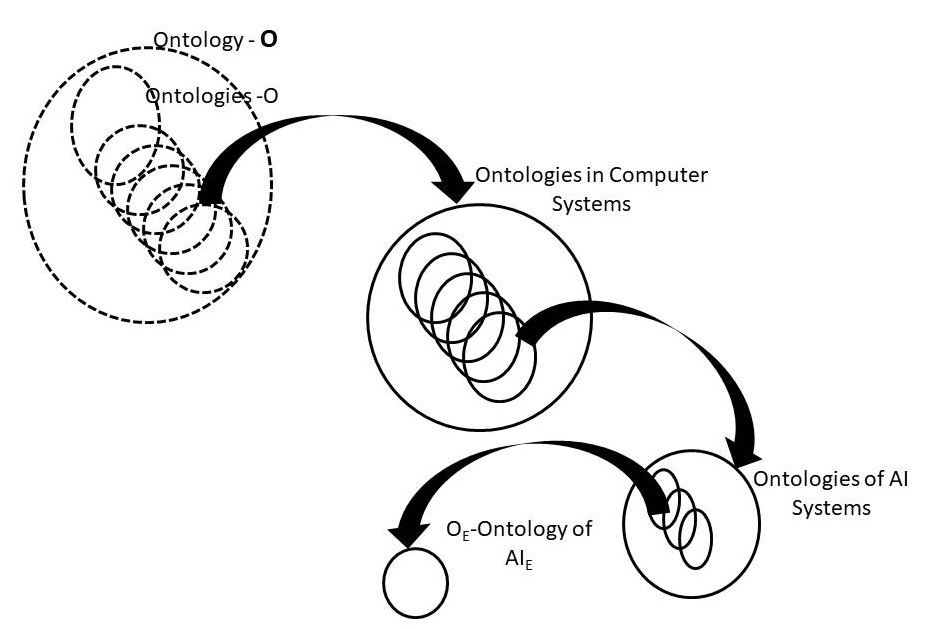
\includegraphics{ART_Krzanowski_Polak/Ontology2200B_pu.jpg}
%\end{figure}
%Figure 1. AI\textsubscript{E} ontology and hierarchy of ontologies.

\begin{figure}[htp]
 \begin{center}
 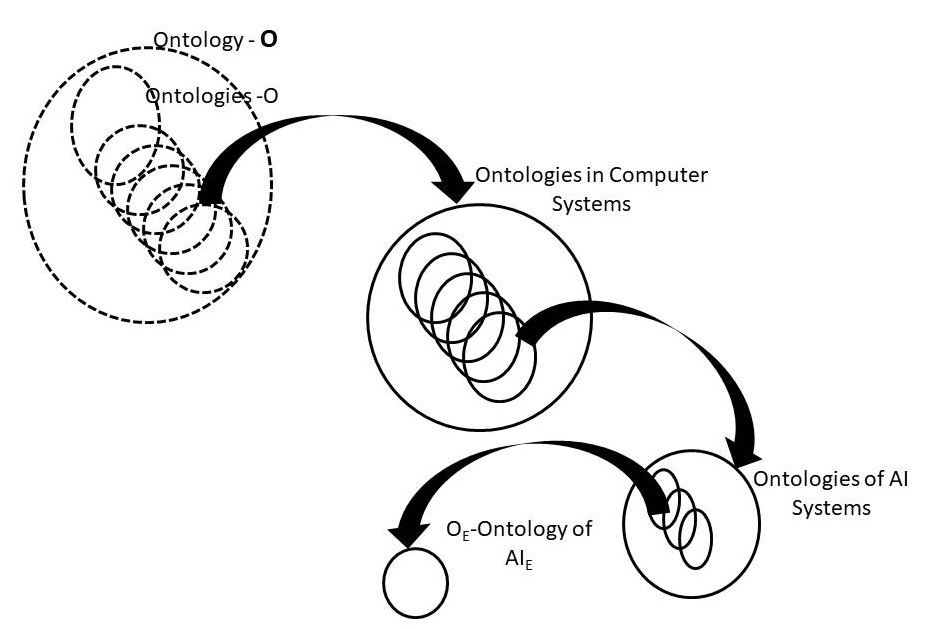
\includegraphics[width=.9\textwidth]{ART_Krzanowski_Polak/Ontology2200B_pu.jpg}%
 \end{center}%
 \caption{AI\textsubscript{E} ontology and hierarchy of ontologies.}\label{krz-ill1}
\end{figure}


Thus, with respect to specificity and scope, O\textsubscript{E} falls under the AI ontologies, which in turn are subspecies of the ontologies of computer systems, and these in turn are forms of specific ontologies (O) concerned with a~specific segment of reality, which then falls under fundamental ontology (\textbf{O}) for existence. All these ontologies ask the same question but within different contexts, scopes, and perspectives. Furthermore, Figure \ref{krz-ill1} shows how only ontology \textbf{O} attempts to comprehend all that exists, with other ontologies being mere fragments. The further away we move from the fundamental ontology \textbf{O}, the narrower and more specific the scope of the ontology becomes.

%Thus, ontology that represents the real world being always expressed in some form of language (which always is) is always incomplete with respect to the world, i.e., the world ``as is'' cannot be represented by something else, despite the close isomorphism between the reality and some logical aka ontological systems \footnote{All pure ontological systems are logical systems
%%\label{ref:RNDQXsIfZlLYA}(Jacquette, 2002, p.xiii; see e.g. Foschini, 2013).
%\parencites[][p.xiii]{jacquette_ontology_2002}[see, e.g.,][]{foschini_where_2013}.%
%}

%%%%%%%%%%%%%%%%%%%%%%%%%%%%%%%%%%%%



Thus, ontology that represents the real world being always expressed in some form of language (which always is) is always incomplete with respect to the world, i.e., the world ``as is'' cannot be represented by something else, despite the close isomorphism between the reality and some logical aka ontological systems.\footnote{All pure ontological systems are logical systems
%\label{ref:RNDQXsIfZlLYA}(Jacquette, 2002, p.xiii; see e.g. Foschini, 2013).
\parencites[][p.xiii]{jacquette_ontology_2002}[see e.g.,][]{foschini_where_2013}.%
} As a~result, there will always be some inconsistency between what exists and what a~given ontology represents, because ontology (even ontology \textbf{O}) will always be a~theory (of sorts), expressed in some specialized language (see ft. 8) about the world rather than the world itself. Thus, there will always be a~degree of incommensurability,\footnote{Incommensurability is not understood here in the same way as the incommensurability of paradigms or scientific theory in the works of Khun 
%\label{ref:RNDg7lp3HNe18}(1962)
\parencite*[][]{kuhn_structure_1962} %
 or Feyerabend 
%\label{ref:RNDdDGQ3TRwiM}(e.g. Ryan, 2002; Sankey, 1993; Oberheim and Hoyningen-Huene, 2018; Bird, 2000).
\parencites[e.g.,][]{ryan_feyerabend_2002}[for the incommensurability of paradigms, see also][]{sankey_kuhns_1993}[][]{oberheim_incommensurability_2018}[][]{bird_thomas_2000}. %
 Instead, incommensurability is understood here as a~general sense of not being entirely comparable according to some criteria.} or a~gap, between the ontology of synthetic systems and the reality of what exists. This gap may be narrowed but never entirely closed. Indeed, a~representation can never contain itself as a~part of what exists. We should keep this incommensurability in mind when building synthetic systems like~AI\textsubscript{E}.

\subsection*{The meta-ontology of AI}

Meta-ontology is a~relatively recently coined term with many interpretations. In philosophy meta-ontology denotes a~study of ontology, what it investigates, and what it is concerned with
%\label{ref:RNDOe0O2QLaGe}(e.g. Quine, 1960; Eklund, 2008; Berto and Plebani, 2015).
\parencites[e.g.,][]{quine_word_1960}[][]{eklund_picture_2008}[][]{berto_ontology_2015}. %
 Peter Van Inwagen 
%\label{ref:RNDlQ2vAbyD19}(1998),
\parencite*[][]{van_inwagen_meta-ontology_1998}, %
 the originator of the term, posited that the role of meta-ontology is to clarify the subject of ontology and explain how ontological claims can be interpreted. Francesco Berto and Matteo Plebani describe meta-ontology in terms of ``‘meta-X' as the inquiry on the central concepts and procedures of discipline X'' 
%\label{ref:RNDRhsH36U3p0}(Berto and Plebani, 2015, p.13),
\parencite[][p.13]{berto_ontology_2015}, %
 where ``X'' refers to ontology in this case. Meta-ontology asks what a~philosopher means when he asks ontological questions or questions about ontology 
%\label{ref:RND0XCU1LJYrl}(Eklund, 2008; Turner, 2014).
\parencites[][]{eklund_picture_2008}[][]{turner_metaontology_2014}. %
 Furthermore, meta-ontology is also concerned with ontological commitments and the truth conditions for a~given ontological theory 
%\label{ref:RNDPFqAz4nWnW}(Van Inwagen, 1998).
\parencite[][]{van_inwagen_meta-ontology_1998}. %
 From this perspective, meta-ontology would inquire as to what kind of ``things'' an ontological theory (i.e., ontology) is committed to.\footnote{We do not discuss Quine's meta-ontology as being specific to Quine's concept of ontology that is not considered here.}

Ontological commitment and truth condition are key terms for defining meta-ontology, and they are critical for differentiating between ontology and meta-ontology
%\label{ref:RNDIMrAPRSpV1}(Turner, 2014).
\parencite[][]{turner_metaontology_2014}. %
 On the conceptual level, the ontological commitment denotes what kind of ontology (i.e., what exists, what is) a~system or a~theory is supposed to represent. Gibson 
%\label{ref:RNDSpom5lKiCH}(2009, p.631)
\parencite*[][p.631]{gibson_ontological_2009} %
 states that ``theory is ontologically committed to an object only if that object occurs in all the ontologies of that theory.'' Thus, ontology may be committed to the existence of numbers, planets, subatomic particles, ghosts, values, ethics, and so on, anything as long as these ``things'' are recognized in ``all the ontologies of that theory'' 
%\label{ref:RND0EJlQmQ9Dk}(e.g. Eklund, 2008).
\parencite[e.g.,][]{eklund_picture_2008}. %
 While ontology is about existence, ``what is'', the ontological commitment is about representation of ``what is'' 
%\label{ref:RNDvi3QcENC1N}(Smith, 1998)
\parencite[][]{smith_origin_1998} %
 and the capacity to represent it.

Moreover, ontological commitment also includes verifying the criteria for this ontological commitment (i.e., verifying the truth of its existential claims). Ontological commitment can be reduced to the simple claim that ``A man is committed to the truth of whatever he asserts''
%\label{ref:RNDA5OgzdmbIa}(Searle, 1969, p.112).
\parencite[][p.112]{searle_speech_1969}.%
\footnote{See the critique of Searle by Inwagen
%\label{ref:RNDdyJS6eDQgJ}(Inwagen, 1991).
\parencite*[][]{lepore_searle_1991}.%
} For some, however, particularly professional ontologists, Searle's take on ontological commitment seems perfunctory, but in the AI context, it provides a~simple (i.e., operational) means for judging the scope of an AI ontology. We do not dispute the robustness of Searle's claim on ontological commitment; here we take it as a~guide in practical applications.

Truth conditions are what makes an ontology correct, such that a~``theory is ontologically committed to an object only if that object occurs in all the ontologies of that theory''
%\label{ref:RND7ceF0NY8f3}(Gibson, 2009, p.631).
\parencite[][p.631]{gibson_ontological_2009}. %
 This statement was rephrased by Rayo 
%\label{ref:RND2olhyVRiGx}(2007)
\parencite*[][]{rayo_ontological_2007} %
 into the following claim: ``[…] for a~sentence to carry commitment to Fs is for the sentence's truth to demand of the world that it contain Fs.'' Gibson's claim therefore comes from a~philosophical perspective. It requires that a~theory (of ontology) can be expressed in sentences (of any language), so this truth condition boils down to an agreement between the theory and the world in question (the correspondence theory of truth\footnote{We are not going here into the discussion of the correspondence theory of truth or truth in general. We assume that for the systems (natural or artificial) ``being in the world'' (no Heideggerian connotations) there must be some relation, however tentative and limited holding between them and the real world they are immersed in, the relation of truth. This relation in a~case of evolution and synthetic systems is verified by systems' operational success 
%\label{ref:RND1clmQWWHtj}(see for example the discussion of truth relation in Bird, 2000).
\parencite[see for example the discussion of truth relation in][]{bird_thomas_2000}. %
 The correspondence theory of truth seems to trouble only philosophers of the anti-realist, skeptical persuasion, not computer scientists or evolutionary biologists 
%\label{ref:RNDL8KkhQlfH3}(Bird, 2000).
\parencite[][]{bird_thomas_2000}. %
 ``Operational success'' in applied sciences may be thought as playing the role of empirical proof in naturalized epistemology 
%\label{ref:RNDDKaQHD0jpK}(Bird, 2000, p.263).
\parencite[][p.263]{bird_thomas_2000}. %
 }), which may be the real world (as is the case of AI\textsubscript{E} systems) or an imaginary constructs or virtual realities whatever the domain of ontology is.

\subsection*{AI\textsubscript{E} Paradigm}

The term ``AI paradigm'' is used in many AI-related papers, discussions, and articles, with it carrying various meanings, so there is no agreement about what it should denote. In principle, authors simply define a~``paradigm'' in a~way that suits their narrative, thus confirming Ian Hacking's prediction that the term would become banal following Kuhn's publication
%\label{ref:RNDbr9uaPs2u1}(Hacking, 2012).
\parencite[][]{kuhn_introductory_2012}. %
 Thus, when we talk about AI paradigm we need to show precisely, to avoid misinterpretations, what we are talking about and how our definition of paradigm differs from, or is similar to, from other definitions.

Schopman
%\label{ref:RNDJc1x1QMFP2}(1986)
\parencite*[][]{schopman_artifical_1986} %
 suggests that AI has not developed a~specific paradigm, claiming that ``[\ldots] no computational paradigm has yet been produced: there is no single generally accepted way to do AI'' 
%\label{ref:RNDPBgq3pJi3C}(Schopman, 1986, p.6).
\parencite[][p.6]{schopman_artifical_1986}. %
 Čaplinskas 
%\label{ref:RNDMRm8DpWtKy}(1998),
\parencite*[][]{caplinskas_ai_1998}, %
 however, defines three AI paradigms: the behaviorist paradigm, the agent paradigm, and the artificial life paradigm. Norvig 
%\label{ref:RNDlOHT6rHNA2}(1992; 2002),
\parencites*[][]{norvig_paradigms_1992}[][]{norvig_retrospective_2002}, %
 meanwhile, associates the term with Lisp programming to express the paradigm of Artificial Intelligence Programming as being equivalent to a~programming approach. Next, Cristianini (2014) distinguishes four AI paradigms: data-driven AI, statistical AI, knowledge-driven AI, and reasoning-and-search-based AI. Without much explanation as to why, Leary 
%\label{ref:RNDMgW31BP6Zx}(2017)
\parencite*[][]{leary_googles_2017} %
 claims that the new Google AI paradigm is machine learning, while in a~blog post titled ``The AI Paradigm Shift,'' Richardson 
%\label{ref:RNDt2zoIcErAM}(2018)
\parencite*[][]{richardson_ai_2018} %
 refers broadly to the AI paradigm as an approach to engineering AI systems, such as deep learning (DL), machine learning (ML), natural language processing (NLP), and robotics. 
%\label{ref:RNDcu5g1TESmD}(Hernández-Orallo et al., 2020, p.2522),
\parencite[][p.2522]{hernandez-orallo_ai_2020}, %
 meanwhile, claims that the concepts of AI paradigms have been used to denote ``broad families of technical or conceptual approaches: ‘symbolic' vs ‘connectionist', reasoning vs learning, expert systems vs agents.''

Much like Richardson, Romero
%\label{ref:RNDPl3RwoIA7v}(2021)
\parencite*[][]{romero_unpopular_2021} %
 refers to deep learning and machine learning as AI paradigms, while Yalçın 
%\label{ref:RNDmyfcw0kayw}(2021)
\parencite*[][]{osaba_artificial_2021} %
 refers to symbolic (i.e., a~human-readable, symbolic representation of problems, logic, and search) and sub-symbolic (i.e., an implicit representation derived from experience-based learning with no symbolic representation of rules and properties) representations as AI paradigms. Villar et al. 
%\label{ref:RNDY4KjMoWStM}(2021)
\parencite*[][]{xu_artificial_2021} %
 hint at relating the AI paradigm to versions of machine-learning and deep-learning methods. Meanwhile, Luhach Kumar and El\c{c}i Atilla 
%\label{ref:RND1BjB3dukU7}(2021)
\parencite*[][]{luhach_artificial_2021} %
 in their book use the term ``paradigm'' in several places but in different contexts, with its meaning being variably associated with programming, the applications of AI to smart computational cyberspaces, or execution paradigms associated with computer hardware. Next, Joseph Makokha 
%\label{ref:RNDS2MHw4L6Mk}(2021)
\parencite*[][]{makokha_artificial_2021} %
 distinguishes two AI paradigms, namely an AI-based one for rule-following methods and another one based on artificial neural network constructs. The term ``AI paradigm'' is often used to simply denote a~method for AI learning or knowledge acquisition, and this is how Yonguin Xu et al. 
%\label{ref:RNDGRGBuNdPMm}(Xu et al., 2021)
\parencite*[][]{xu_artificial_2021} %
 use this term to denote~deep-learning approaches, such as supervised, unsupervised, and reinforced learning.

Several studies have posited that the current AI systems use two broad, conceptual constructs, namely the symbolic and the sub-symbolic
%\label{ref:RNDiWrk1ACHd1}(e.g. Searle, 1998; Harvey, 2013; Neapolitan and Jiang, 2018; Mitchell, 2019; Smith, 2019; Cole, 2020; Russell and Norvig, 2020; Wooldridge, 2021).
\parencites[e.g.,][]{searle_mind_1998}[][]{harvey_perspectives_2013}[][]{neapolitan_artificial_2018}[][]{mitchell_artificial_2019}[][]{smith_promise_2019}[][]{cole_chinese}[][]{russell_artificial_2020}[][]{wooldridge_road_2021}. %
 Thus, the symbolic paradigm reflects symbolic representations of a~priori defined concepts that may be implemented in various programming environments, while the sub-symbolic paradigm relates to less clearly defined concepts, such as the multi-dimensional probability weights on the connections within an artificial neural network. An approach under the sub-symbolic paradigm would therefore be implemented using one of the various machine learning (ML) technologies. These two paradigms can also be fused into a~neuro-symbolic paradigm 
%\label{ref:RNDTv0qtZz01g}(e.g. Bader and Hitzler, 2005; Garcez et al., 2019; Garcez and Lamb, 2020; Kautz, 2022)
\parencites[e.g.,][]{bader_dimensions_2005}[][]{garcez_neural-symbolic_2019}[][]{garcez_neurosymbolic_2020}[][]{kautz_third_2022} %
 that combines symbolic and sub-symbolic elements. As pointed out earlier, the term ``AI paradigm'' does not point to a~single software or hardware solution 
%\label{ref:RNDzI0NRHZm9F}(see Minsky, 1991; Russell and Norvig, 2020)
\parencites[see][]{minsky_logical_1991}[][]{russell_artificial_2020}.%

In this paper, we follow the example of Searle, Harvey, Neapolitan and Jiang, Smith, Cole, Wooldrige, and Russell and Norwig in using the term ``AI paradigm'' to denote a~broad, conceptual construct that underlies AI systems. AI paradigm as is here defined does not imply a~specific implementation. The AI paradigm therefore allows for multiple implementations, formal structures, representations, programming methods, and processing algorithms,\footnote{We use the term algorithm in the general sense of a~procedure that can be conceptualized and implemented in a~computer. This use follows Knuth's definition of a~computational method as being ``A procedure that has all of the characteristics of an algorithm except that it possibly lacks finiteness may be called a~computational method''
%\label{ref:RNDXsmzRWvSXf}(Knuth, 2005, p.5).
\parencite[][p.5]{knuth_art_2005}.%
} with these all belonging to a~single paradigm.

\section*{The meta-ontology of AI\textsubscript{E} systems}
We have concluded that in philosophy, meta-ontology is the study of what ontology is all about. In other words, it is a~study of, or about, ontology, as well as what it investigates; after Berto and Plebani ``‘meta-X' as the inquiry on the central concepts and procedures of discipline X'', where ``X'' refers to ontology in this case
%\label{ref:RNDc30wpAwAYr}(Berto and Plebani, 2015, p.13).
\parencite[][p.13]{berto_ontology_2015}. %
 We also concluded that ontological commitment and truth conditions represent the key concepts of meta-ontology, and these terms are critical for differentiating between ontology and meta-ontology.

The meta-ontology of AI\textsubscript{E} systems retains the core philosophical meaning (i.e., what ontology is committed to), but it diverges from the philosophical concept in the details, because it assumes the perspective of AI\textsubscript{E} systems. When we say it ``retains the core philosophical meaning,'' we mean that meta-ontology of AI\textsubscript{E} systems is concerned with ontology, or is about ontology (i.e., the philosophical meaning of meta-ontology). Contrary to the use in philosophy, however, the meta-ontology of the AI\textsubscript{E} focuses not on a~theory of ontology, as meta-ontologies in philosophy do, but rather on what the AI\textsubscript{E} represents (i.e., the real world).

We also said that we are concerned with studying the meta-ontology of the AI\textsubscript{E} paradigm, which is the broad all-encompassing conceptual construct that underlies AI\textsubscript{E} systems, rather than any particular realization of it. Indeed, we assume that most realizations of AI\textsubscript{E} systems have the same foundational assumptions; what we denote as AI\textsubscript{E} systems paradigm, so what we can conclude about the ontology of AI\textsubscript{E} paradigm will also hold for its realizations. Different paradigms (from the one assumed here) of AI\textsubscript{E} systems are logically possible. But we limit this discussion to assumptions, formulated by Smith, that AI\textsubscript{E} systems should possess if they are to mimic humans' ability to cope with the real world (i.e., have human-level intelligence).

Summing this all up, the meta-ontology of the AI\textsubscript{E} paradigm\footnote{The discussion of the meta-ontology of the AI\textsubscript{E} paradigm is based on ideas proposed by Brian Cantwell Smith
%\label{ref:RNDOjQKQUXhkH}(1998; 2019)
\parencites*[][]{smith_origin_1998}[][]{smith_promise_2019} %
 and the works of Minsky 
%\label{ref:RNDcsIm1syif4}(1991),
\parencite*[][]{minsky_logical_1991}, %
 Dreyfus 
%\label{ref:RNDdI8HiC51kr}(2016),
\parencite*[][]{dreyfus_skillful_2016}, %
 Mitchell 
%\label{ref:RNDTfVWKoSNl0}(2019),
\parencite*[][]{mitchell_artificial_2019}, %
 Roitblat 
%\label{ref:RNDsAzvS6rrzl}(2020),
\parencite*[][]{roitblat_algorithms_2020}, %
 and Wooldridge 
%\label{ref:RNDvNRoiypAst}(2021).
\parencite*[][]{wooldridge_road_2021}.%
} is concerned primarily with what is (or about) the ontology of AI\textsubscript{E} systems, what its ontological commitment is, and what its truth condition~is.

To make our claims about the ontology of AI\textsubscript{E} systems more specific, we employ Smith's postulates for the AI\textsubscript{E} paradigm
%\label{ref:RND29u62Bbbh8}(Smith, 2019, p.44).
\parencite[][p.44]{smith_promise_2019}. %
 As we mentioned earlier, Smith's AI\textsubscript{E} paradigm is not purely ontological, but it does commit AI\textsubscript{E} systems to certain ontology. Smith posited that for an AI system to match human-level intelligence, it needs to be embodied, embedded, extended, and enactive. More specifically, embodied means that an AI\textsubscript{E} agent's representation of the real world accounts for its body's position, size, senses, and movement, such that the body plays a~critical role in shaping the ``mind'' and its internal representation of the world (i.e., embodied cognition). Extended, meanwhile, implies that the AI\textsubscript{E} agent's representation of the real world accounts for the AI\textsubscript{E} system's mind and body as part of the cognition process (i.e., a~co-creating ontology). (For more about the discussion of embodied and extended cognition, see, for example, the works of Varerla 
%\label{ref:RNDvCXrAhdWw2}(1991),
\parencite*[][]{varela_embodied_1991}, %
 Clark and Chalmers 
%\label{ref:RND3YztrV28fq}(1998),
\parencite*[][]{clark_extended_1998}, %
 Anderson 
%\label{ref:RNDuPfTPiR4o2}(2003),
\parencite*[][]{anderson_embodied_2003}, %
 Pfeifer and Iida 
%\label{ref:RNDl6Q4xbxe4U}(2004),
\parencite*[][]{pfeifer_embodied_2004}, %
 Rupert 
%\label{ref:RNDcvGFRfhEoC}(2009),
\parencite*[][]{rupert_cognitive_2009}, %
 Rowland 
%\label{ref:RNDkeNjWoXyQs}(2010),
\parencite*[][]{rowlands_new_2010}, %
 Shapiro 
%\label{ref:RNDED0HOeVh1y}(2010),
\parencite*[][]{shapiro_embodied_2010}, %
 Wheeler 
%\label{ref:RNDoWYqvEJslZ}(2011),
\parencite*[][]{garvey_embodied_2011}, %
 Kiverstein 
%\label{ref:RNDwQlQCbODVD}(2018),
\parencite*[][]{kiverstein_extended_2018}, %
 Bermúdez 
%\label{ref:RND1GyfYpOKD4}(2020),
\parencite*[][]{hernandez-orallo_ai_2020}, %
 and Paul 
%\label{ref:RNDIu9EsGLB3m}(2021)
\parencite*[][]{paul_extended_2021}%
). Next, the embedded condition refers to the AI\textsubscript{E} system being aware of the context surrounding a~situation, which should be accounted for in its ontology 
%\label{ref:RNDyenofiyHeN}(e.g. Hutchins, 1995; Pouw, van Gog and Paas, 2014).
\parencites[e.g.,][]{hutchins_cognition_1995}[][]{pouw_embedded_2014}. %
 Finally, being enactive means that an AI\textsubscript{E} agent fully participates in actions, both in mind and body 
%\label{ref:RND8zIILWJS7n}(e.g. Varela, Thompson and Rosch, 1991, p.175; Klein, Moon and Hoffman, 2006; Froese and Ziemke, 2009; ``the brain is conceived as participating in the action'' Gallagher et al., 2013; Di Paolo and Thompson, 2017; Hutto and Myin, 2017; Newen, De Bruin and Gallagher, 2018; Smith, 2019; Newen, Bruin and Gallagher, 2020; Käufer and Chemero, 2021; Shapiro and Spaulding, 2021; ``enacted AI'' Shin, 2021; Hipólito and van Es, 2022).
\parencites[e.g.,][p.175]{varela_embodied_1991}[][]{klein_making_2006}[][]{froese_enactive_2009}[``the brain is conceived as participating in the action''][]{gallagher_brain_2013}[][]{di_paolo_enactive_2017}[][]{hutto_evolving_2017}[][]{newen_4e_2018}[][]{smith_promise_2019}[][]{newen_oxford_2020}[][]{kaufer_phenomenology_2021}[][]{shapiro_embodied_2021}[``enacted AI''][]{shin_embodying_2021}[][]{hipolito_enactive-dynamic_2022}.%


Still, it is not obvious what ontology is implied by these requirements. As well as, it is not obvious, as to how we should translate the four features of this AI\textsubscript{E} paradigm into meta-ontological requirements; Smith neglects to offer any suggestions here
%\label{ref:RNDo0hvs3R1Nz}(Smith, 1998; 2019).
\parencites[][]{smith_origin_1998}[][]{mitchell_artificial_2019}. %
 Thus, we reformulated Smith's claims about the ontology of AI\textsubscript{E} systems into four meta-ontological theses that appear to fill the ontological lacuna in his specifications. Indeed, they would seem to be necessary for AI\textsubscript{E} systems to be embodied, embedded, extended, and enactive. They are:
%\textit{T1. The ontological commitment of AI}\textit{\textsubscript{E}}~\textit{is to the real world, the world of a~human agent.}
%
%\textit{T2. The truth condition of the ontology of AI}\textit{\textsubscript{E}} \textit{is not consistency with ontological theory but rather the real world.}
%
%\textit{T3. The truth condition of AI}\textit{\textsubscript{E}} \textit{is verified through the operational success of an AI}\textit{\textsubscript{E}} \textit{system.}
%
%\textit{T4. The ontology of the AI}\textit{\textsubscript{E}} \textit{paradigm must account for the dynamic environment of the real world.}
\begin{enumerate}[label=T\arabic*.]
\item The ontological commitment of AI\textsubscript{E} is to the real world, the world of a~human agent.
\item The truth condition of the ontology of AI\textsubscript{E} is not consistency with ontological theory but rather the real world.
\item The truth condition of AI\textsubscript{E} is verified through the operational success of an AI\textsubscript{E} system.
\item The ontology of the AI\textsubscript{E} paradigm must account for the dynamic environment of the real world.
\end{enumerate}


%(\textbf{T1) The ontological commitment of AI}\textbf{\textsubscript{E}}~\textbf{is to the real world,}\footnote{The term explained earlier in the text.}
%\textbf{the world of a~human agent}:
\paragraph[(T1) The ontological commitment]{(T1) The ontological commitment of AI\textsubscript{E} is to the real world,\footnote{The term explained earlier in the text. See footnote 7.} world of a~human agent.}%
 The world for AI\textsubscript{E} is the same reality that a~human actor would exist in. We could say that AI\textsubscript{E} ontology is a~partial ontology as opposed to one that covers the entire world, so it is about a~state of affairs, by which we mean a~local, temporal, dynamic (as described by Minsky) reality of the everyday world. This partial ontology does not attempt to create a~comprehensive ontology of existence but rather account for what exists, together with the state of affairs,\footnote{The term ``state of affairs'' is used in the sense employed by Jacquette
%\label{ref:RNDlvlS6tqNBF}(2002).
\parencite*[][]{jacquette_ontology_2002}.%
} in the part of the actual world that is relevant to an AI\textsubscript{E} agent, we may say, agent-relevant ontology.

AI\textsubscript{E} ontology is therefore not a~theory about what exists, abstract objects, possible worlds, and maximal worlds
%\label{ref:RND3mxjMlPNzS}(e.g. Forbes, 1992; Textor, 2021).
\parencites[e.g.,][]{mulligan_worlds_1992}[][]{textor_states_2021}. %
 Indeed, rejecting models or theories about the world may be beneficial, as Brooks suggests (in her ontology of everyday objects): ``When we examine very simple level intelligence we find that explicit representations and models of the world simply get in the way. It turns out to be better to use the world as its own model'' 
%\label{ref:RNDqqGsiV7pPi}(Brooks, 1991).
\parencite[][]{brooks_intelligence_1991}. %
 For instance, the ontology of the AI\textsubscript{E} paradigmmay not have to account for subatomic particles, quantum physics, or imaginary objects, so it does not have to resolve Russell's table paradox 
%\label{ref:RNDIbsawWdln9}(Russell, 1912);
\parencite[][]{russell_problems_1912}; %
 it does not have to account for these or similar objects as it is an ontology of everyday world we live in (it is Minsky's commonsense reality, or Baker's the world of ordinary things, or ``the world of medium–sized objects'' 
%\label{ref:RNDeJSmfq0gW8}(Baker, 2007, p.18)
\parencite[][p.18]{baker_metaphysics_2007}%
).

Accordingly, the ontological commitment of the AI\textsubscript{E} paradigm is whatever an AI\textsubscript{E} system can assert about the world (i.e., the entities, relations between them, etc.) given its paradigm. AI\textsubscript{E} systems face the real world, so they are committed to things within their context, and they need to recognize reality's features. Thus, the ontological commitment in AI\textsubscript{E} systems that seek to mimic our own ontological commitment must be geared toward recognizing the reality with limited \textit{a~priori} suppositions.\footnote{See also Käufer and Chemero's
%\label{ref:RNDMHSUwWgUV8}(2021, p.220)
\parencite*[][p.220]{kaufer_phenomenology_2021} %
 discussion of Heideggerian AI, which is very similar to Baker's ontology of ordinary things 
%\label{ref:RND8iYIh5Ylaa}(Baker, 2007)
\parencite[][]{baker_metaphysics_2007} %
 and a~critique of the representational approach to the world.}

%(\textbf{T2) The truth condition of AI}\textbf{\textsubscript{E}} \textbf{is not consistency with ontological theory but rather the real world.
\paragraph{(T2) The truth condition of AI\textsubscript{E} is not consistency with ontological theory but rather the real world.}
The truth condition of \textbf{AI}\textbf{\textsubscript{E}} \textbf{systems} does not depend on theory, and it is not committed to the truth of a~sentence because there are no sentences or collections of them, as there is no \textit{a~priori} ontological theory defining the ontology of \textbf{AI}\textbf{\textsubscript{E}} \textbf{systems}. The truth condition of \textbf{AI}\textbf{\textsubscript{E}} \textbf{systems}' ontology is therefore not consistency with a~closed conceptual schema or ontological theory but rather with reality, with ``what is the world like''
%\label{ref:RNDkXiflYvHcu}(Smith, 2019, p.57).
\parencite[][p.57]{smith_promise_2019}.%


The truth condition of the AI\textsubscript{E} paradigm shares some similarities with the truth condition of philosophy, which states that ``theory is ontologically committed to an object only if that object occurs in all the ontologies of that theory''
%\label{ref:RNDe7Qk8dHvAr}(Gibson, 2009, p.631).
\parencite[][p.631]{gibson_ontological_2009}. %
 Or, in and alternative formulation by Rayo 
%\label{ref:RNDez2d7KVZBH}(Rayo, 2007)
\parencite*[][]{rayo_ontological_2007} %
 rephrased as follows: ``for a~sentence to carry commitment to Fs is for the sentence's truth to demand of the world that it contain Fs.'' However, the truth condition of AI\textsubscript{E} systems requires AI systems to ``deal with reality as it actually is---not in the way our language represents it as being'' 
%\label{ref:RNDPlQIuEJgnp}(Smith, 2019, p.34),
\parencite[][p.34]{smith_promise_2019}, %
 i.e., the truth condition of AI\textsubscript{E} systems does not have to satisfy any sentences; understood as the ontological claims expressed in some form of language.

%(\textbf{T3) The truth condition of AI}\textbf{\textsubscript{E}} \textbf{systems} \textbf{is verified through operational success}.
\paragraph{(T3) The truth condition of AI\textsubscript{E} systems is verified through operational success.}
The truth condition of \textbf{AI}\textbf{\textsubscript{E}} \textbf{systems} is not concerned with computational representations of reality in the form of structures, data constructs, or computational concepts. Objects that are registered in \textbf{AI}\textbf{\textsubscript{E}} \textbf{systems} follow~constitutive regularities and norms, but these are not known beforehand but instead derived and learned from the real world as the basis of being
%\label{ref:RNDlXo6W1ixLP}(Smith, 2019, p.103).
\parencite[][p.103]{smith_promise_2019}. %
 There is no theory to go with it, so there is no criterion for truth verification that references a~theory, at least if we accept that this statement is not a~theory in itself. As Baker says in an article about the metaphysics of ordinary things, ``the ultimate test of a~metaphysical theory is\ldots pragmatic'' 
%\label{ref:RNDPeMuxppH4c}(Baker, 2007, p.11).
\parencite[][p.11]{baker_metaphysics_2007}.%
\footnote{In Baker's ontology, the pragmatic mode of verification has nothing to do with pragmatic theories of truth in philosophy.} In other words, the truth condition of AI\textsubscript{E} systems is verified pragmatically, i.e., through operational success, because they are solely committed to the world and their actions within it 
%\label{ref:RNDPFPJ38CJSH}(Smith, 2019, p.145).
\parencite[][p.145]{smith_promise_2019}. %
 The precise meaning of operational success of engineering (including AI\textsubscript{E} systems) or natural systems (living organisms) depend on the specific system the term ``operational success'' is applied to. In biological systems operational success (mostly) means survival and reproduction. In artificial systems operational success means fulfilling design objectives. It is not always obvious what is operational success even in engineering systems. For factory robots operational success is a~well-defined task -- like proper welding of a~pin or similar. For autonomous vehicles operational success means (among other things) collision avoidance. For AI\textsubscript{E} systems operational success is proper response/decision to situations. Of course operational success is much harder to evaluate in some cases than a~welding of a~pin; like it is in a~case of the notorious trolley problem 
%\label{ref:RNDFJRT1yhI7Z}(see e.g. Cathcart, 2013).
\parencite[see e.g.,][]{cathcart_trolley_2013}. %
 ``Operational success'' of the trolley problem is a~subject of endless debates between engineers, philosophers and enthusiasts of AI probably with a~limited chance of success as these groups talk past each other; philosophers see the trolley problem as ethical problems, engineers as engineering problem, and enthusiasts of AI are too emotionally engaged to be rational. As we mentioned earlier, registered/recognized objects in \textbf{AI}\textbf{\textsubscript{E}} \textbf{ontology} create regularities and norms, but rather than being known a~priori, they are derived and learned from the real world, and this provides the grounding for AI\textsubscript{E} ontology.

%(4)\textbf{ The ontology of AI}\textbf{\textsubscript{E}} \textbf{systems must account for the dynamic environment of the real world}
\paragraph{(T4) The ontology of AI\textsubscript{E} systems must account for the dynamic environment of the real world.}
The complex and dynamic nature of the AI\textsubscript{E}~domain was discussed by Minsky: ``\ldots the objects and activities of everyday life are too endlessly varied to be described by precise, logical definitions and deductions. Commonsense reality is too disorderly to represent in terms of universally valid axioms. To account for such variety and novelty, we need more flexible styles of thought, such as those we see in human commonsense reasoning, which is based more on analogies and approximations than on precise formal procedures''
%\label{ref:RNDTUfu96TfPX}(Minsky, 1991, p.6).
\parencite[][p.6]{minsky_logical_1991}.%
\footnote{Minsky is obviously not the first or only person to recognize the messiness of reality, but he is one of the few AI researchers that did so in the early years of AI technology (others include, for example, Dreyfus 
%\label{ref:RND3JyKB3OghV}(2016),
\parencite*[][]{dreyfus_skillful_2016}, %
 Wooldridge 
%\label{ref:RNDG0axi4Lh6W}(2021),
\parencite*[][]{wooldridge_road_2021}, %
 Smith 
%\label{ref:RNDSdLeJwOOfh}(2019),
\parencite*[][]{smith_promise_2019}, %
 Bołtuć 
%\label{ref:RNDPjPFdTs0bm}(2020),
\parencite*[][]{boltuc_conscious_2020}, %
 Mitchell 
%\label{ref:RND4efPhb346l}(2019),
\parencite*[][]{mitchell_artificial_2019}, %
 Roitblat 
%\label{ref:RNDIlIa1h1a1b}(2020),
\parencite*[][]{roitblat_algorithms_2020}, %
 and Käufer and Chemero 
%\label{ref:RND74fIR1Q2nQ}(2021)
\parencite*[][]{kaufer_phenomenology_2021}%
).}

Thus, the reality that the ontology of the AI\textsubscript{E} paradigm must represent is specific to a~situation, because raw reality is too disorderly to represent through universally valid axioms. Indeed, the reality/ontology faced by AI\textsubscript{E} is too complex and nuanced to be definable by a~closed set of formal rules, and any attempt to do so would result in a~combinatorial explosion
%\label{ref:RND7flUBMt0hf}(Inder, 1996, p.26).
\parencite[][p.26]{inder_planning_1996}. %
 This combinatorial explosion barrier implies that the ontology of the AI\textsubscript{E} paradigm must eschew any formal \textit{a~priori} decision-making procedures.\footnote{Philosophical ontology recognizes that (to some extent) the needs of AI\textsubscript{E} ontology seem to be the ``ontology of everyday life'' described by 
%\label{ref:RNDmyE1FLYebC}(Baker, 2007).
\parencite[][]{baker_metaphysics_2007}. %
 Baker describes the ontology of common objects (i.e., the ``metaphysics of everyday objects''), and this ontology may provide a~philosophical interpretation for AI\textsubscript{E} ontology, but possible similarities would again require further study.}

We remain unsure about how to design AI systems that implement Smith's embodied, embedded, extended, and enactive ontology
%\label{ref:RNDKos62epxtR}(e.g. Hoffmann and Pfeifer, 2018).
\parencite[e.g.,][]{hoffmann_robots_2018}. %
 Nevertheless, as biological agents do have embodied, embedded, extended, and enactive ontology suited to their specific living niche, we can assume that, in principle, synthetic systems could do the same, at least to some degree and perhaps with the use of technology that may not yet exist.\footnote{Smith's concept is similar to 4E cognition 
%\label{ref:RNDBchKG0UeaL}(e.g. Shapiro, 2010; Wheeler, 2011; Newen, Bruin and Gallagher, 2020).
\parencites[e.g.,][]{shapiro_embodied_2010}[][]{garvey_embodied_2011}[][]{newen_oxford_2020}. %
 The field of 4E cognition requires a~separate discussion because it lies outside the scope of this paper.}

\section*{Conclusions }
In summation, the meta-ontological claims about AI\textsubscript{E} systems posit that the ontological commitment of an \textbf{AI}\textbf{\textsubscript{E}} system is directed solely to the outside world. In addition, the truth condition of \textbf{AI}\textbf{\textsubscript{E}} \textbf{systems}' ontology is not consistency with a~closed conceptual schema or ontological theory but rather with the reality, with ``what is the world''
%\label{ref:RNDaSQKcsJIDD}(Smith, 2019, p.57).
\parencite[][p.57]{smith_promise_2019}. %
 It is not concerned with computational representations of reality in the form of structures, data constructs, or computational concepts. In addition, this truth condition of \textbf{AI}\textbf{\textsubscript{E}} \textbf{systems} is verified through operational success.

We are well aware of how natural systems engage successfully (most of the time) with the real world, and we know, at least in some sense, how they achieve this (see, for example, studies of 4E cognition
%\label{ref:RNDxRkjOFKUxi}(Shapiro, 2010; Wheeler, 2011; Newen, Bruin and Gallagher, 2020)
\parencites[][]{shapiro_embodied_2010}[][]{garvey_embodied_2011}[][]{newen_oxford_2020} %
 or the work of Yong 
%\label{ref:RNDY924WljM6t}(2022)
\parencite*[][]{yong_immense_2022}%
). To replicate the prowess of natural systems in synthetic systems, at least to some extent, we know that we need to mimic what natural systems do (i.e., engage with the real world 
%\label{ref:RNDcLhP3ThSeQ}(see e.g. Sarosiek, 2021)
\parencite[see e.g.][]{sarosiek_role_2021}%
). In fact, we do not have any other example to follow but us and some other animals.

We also know that we must do something different to the way in which we approach AI systems now. In other words, we must change our AI paradigm, i.e., foundational assumptions about constructing AI systems (We refer again to the ideas of Minsky
%\label{ref:RNDw8x3teCm3a}(1991),
\parencite*[][]{minsky_logical_1991}, %
 Dreyfus 
%\label{ref:RNDmWthEZEHwe}(2016),
\parencite*[][]{dreyfus_skillful_2016}, %
 Wooldridge 
%\label{ref:RNDoggJMn5SGJ}(2021),
\parencite*[][]{wooldridge_road_2021}, %
 Smith 
%\label{ref:RNDYCPWPtaVOp}(2019),
\parencite*[][]{smith_promise_2019}, %
 Mitchell 
%\label{ref:RNDEMFWgkuA5M}(2019),
\parencite*[][]{mitchell_artificial_2019}, %
 and Roitblat 
%\label{ref:RNDzdtFcNjNAc}(2020).
\parencite*[][]{roitblat_algorithms_2020}.%
) Alas, we still do not know how to do this effectively.

We also know that we will always have a~degree of incommensurability between the ontology of synthetic systems (including AI\textsubscript{E} systems) and reality, which is in a~sense explained in ft. 8, because there is also insurmountable incommensurability between the ontology of biological agents and reality. This means there will always be some shortfall between what exists and what can be comprehended by a~system, whether biological or synthetic
%\label{ref:RNDfEtfOyq3L8}(e.g. Yong, 2022).
\parencite[e.g.,][]{yong_immense_2022}. %
 Indeed, the ontology of a~cognitive agent, whether natural or synthetic, always only partially covers reality (revisit Figure 1), because for biological systems, it is tailored to its environmental niche and continued survival, while for synthetic systems, it is oriented toward ensuring the utility of a~system and the safety of those related to, on relaying on, this system. The best we can do is to minimize this incommensurability gap, once we realize that it exists, by optimizing a~system to suit a~specific environment.

Indeed, the meta-ontological lesson from nature is not that organisms strive to match their ontology with \textbf{O}~ontology but rather to optimize their ontology to best meet their needs
%\label{ref:RNDD6ChPn1yKu}(see e.g. Yong, 2022)
\parencite[see e.g.,][]{yong_immense_2022} %
 or occupy their biological niche, although this niche is essentially what their ontology is. Is this the way to go for AI\textsubscript{E} systems? Obviously, a~factory robot tightening nuts and bolts does not need an AI\textsubscript{E} ontology, but a~robot delivering pizza in a~city would require a~more sophisticated ontology. And so would police robots with the license to kill patrolling the city streets 
%\label{ref:RNDCgwWBDNJAY}(see e.g. Propper, 2022).
\parencite[see e.g.,][]{propper_san_2022}. %
 Furthermore, robotic companions, nurses, or personal assistants may require a~still higher level of AI\textsubscript{E} ontology. Such robots would need to navigate the messy environment of everyday life with the sort of cleverness that we expect from their human counterparts. In other words, they need human-level intelligence with human-level ontology.

The meta-ontological perspective, in the absence of generally accepted criteria, may also be useful for defining the AI paradigm, which could then be differentiated not by computing methods, software, or theories (as it is the case now) but rather by the ability to represent the real world. Such a~perspective would clearly separate symbolic, sub-symbolic, or neuro-symbolic systems from their \textbf{AI}\textbf{\textsubscript{E}} peers.\footnote{Meta-ontology has been used as a~differentiating criterion between ontological paradigms. For example, Eklund
%\label{ref:RNDV2s3Rdx8HA}(2008)
\parencite*[][]{eklund_picture_2008} %
 uses meta-ontology to differentiate between ontological paradigms, such as between robust and deflationary conceptions of ontology.}




\end{artengenv2auth}
\label{krzanowpolak_stop}
%
\begin{document}
\title{Is Information Ontological or Physical, or Is It Perhaps Something Else? Some Remarks on Krzanowski's Approach to the Concept of Information}
\maketitle

Łukasz Mścisławski

Politechnika Wrocławska

\url{https://orcid.org/0000-0003-0195-906}

\section{Abstract}
As one may have noticed, the title of this paper is somewhat provocative. We found Roman Krzanowski's
%\label{ref:RNDD4ZPbWpWxt}(2020a; 2020b; 2020c; 2022)
\parencites*[][]{krzanowski_does_2020}[][]{krzanowski_what_2020}[][]{krzanowski_why_2020}[][]{krzanowski_ontological_2022} %
 proposed approach to the problem of information very intriguing. Our aim here is to highlight some advantages when it comes to answering some fundamental questions in the philosophy of physics and metaphysics, as well as the philosophy of information and computer science. This issue is of great importance, so we propose that the introduction of some subtle distinctions between ontological and epistemological information can be regarded as being analogous to G.F.R. Ellis's analyses of the passage of time in his concept of the Crystallizing Block Universe 
%\label{ref:RNDaS7kEBPadF}(Ellis and Goswami, 2012).
\parencite[][]{ellis_space_2012}. %
 This analogy could be useful when further studying the relations between different types of information. We also suggest some subjects for further study, ones where Krzanowski's proposal could serve as a~very solid foundation for examining traditional metaphysical issues by combining classical philosophical doctrines with the new approach.

\section{Introduction}
This article primarily aims to concisely present Roman Krzanowski's approach to the concept of \textit{physical information.} This concept is perceived here as a~kind of ``intermediate concept'' that can act as a~bridge to the development of his concept of \textit{ontological information}
%\label{ref:RNDVGZ8jlBX2V}(cf. Krzanowski, 2020a; 2020b; 2020c; 2022),
\parencites[cf.][]{krzanowski_does_2020}[][]{krzanowski_what_2020}[][]{krzanowski_why_2020}[and especially][]{krzanowski_ontological_2022},%
and can be regarded as a~special case of the latter. Indeed, we believe that the latter concept inherits many characteristics from the former, but not all the issues have been solved.\footnote{It is also worth mentioning that in some works, Krzanowski seems to use these two terms (i.e., physical and ontological information) interchangeably
%\label{ref:RNDx2sgo6ehaO}(cf. Krzanowski, 2020b).
\parencite[cf.][]{krzanowski_what_2020}.%
} This situation implies that we are dealing with a~truly fundamental issue here, namely the fundamentality of the concept of information. Furthermore, this paper also aims to discuss some of this concept's interesting properties and present possible avenues for further developing this interesting proposal. It is well known that there is enormous interest in the philosophical aspects of the concept of information 
%\label{ref:RNDKUzkfsqSdA}(e.g. Adriaans and Benthem, 2008; Burgin, 2010; Floridi, 2011; Dodig Crnkovic and Burgin, 2019),
\parencites[e.g.,][]{adriaans_philosophy_2008}[][]{burgin_theory_2010}[][]{floridi_philosophy_2011}[][]{dodig_crnkovic_philosophy_2019}, %
 but we feel that Krzanowski's proposal is particularly attractive with some great research potential, especially for studying physical reality. It would %
therefor be helpful, in our opinion, to position this concept within the vast array of philosophical problems related to the notion of information, as well as introduce a~few distinctions to allow us to order the discourse.

The first distinction we would like to introduce, because we consider it important, is the distinction between two perspectives for the notion of information:

\begin{enumerate}
\item Ontological; and
\item Epistemological.
\end{enumerate}
These two areas of research are by no means mutually exclusive, but they pose slightly different kinds of questions. Krzanowski
%\label{ref:RNDf3GlACHwY4}(2020c, pp.37–38; 2022, pp.123–151)
\parencites*[][pp.37–38]{krzanowski_why_2020}[][pp.123–151]{krzanowski_ontological_2022} %
 presented an analogous distinction.\footnote{A~slightly different version is also presented in 
%\label{ref:RNDU9el6H16Mu}(Krzanowski, 2020b),
\parencite[][]{krzanowski_what_2020}, %
 where a~distinction between abstract and concrete information is introduced. There is a~little more on this subject below.} \textcolor{black}{For the purposes of this paper, however, they can be characterized as follows: The }\textit{\textcolor{black}{ontological}}\textcolor{black}{ (A) perspective mainly poses questions about what something is, how it exists, what its inherent properties are, and so on. It is worth noting here that within this research area, it is possible to pose a~question about the general structure of reality (i.e., its ontology and the ``location'' of information within it) and thus its ontological status. Such a~general perspective makes it possible to regard information as something tangible, so there is no need to reify it, although we cannot exclude such a~possibility. This perspective is of particular interest to Krzanowski and therefore also to this paper.}\footnotetext{As a~rule in this paper, ontology is not understood as a~network of concepts and relations between them, as is the case in some formal disciplines.}


The \textit{epistemological} (B) perspective, on the other hand, poses questions that are typical of epistemology, such as how something can be cognitively grasped and whether and how it relates to issues of knowledge, truth, cognition, and so on.

The second distinction that naturally arises when considering the notion of information relates to two approaches:

\begin{enumerate}
\item Qualitative; and
\item Quantitative.
\end{enumerate}
It is plain to see that these two approaches can be combined with the above perspectives. We could say that the epistemological perspective (B) is compatible with both approaches (I and II). Similarly, it is clear that perspective A~must be compatible with approach I. Nevertheless, some interesting issues arise:

\begin{enumerate}
\item Can every characteristic of I~be expressed in the form of II? It seems that the answer to this question is by no means obvious, and trying to provide one may be better regarded as a~starting point for some interesting and deep research into addressing the general problem of relating the two approaches.
\item Is it possible to combine perspective A~with approach II for the concept of information? This is not something that could be achieved by simply declaring that ``information is quantitative only''. It seems that any serious attempt to answer this sort of question would possibly require connecting what we call \textit{information} with mathematical structures. Perhaps with regard to the ontological status of the latter, a~perspective along the lines of mathematical Platonism should be included here, at least to some extent.
\end{enumerate}
It is also worth noting another difficulty with approaches of type II, which can be formulated as follows: \textit{What is that} which is being quantitatively represented? This question becomes all the more pertinent when one accounts for Burgin's
%\label{ref:RNDXJtOCj8zkW}(2011, p.349)
\parencite*[][p.349]{burgin_information_2011} %
 observation, where the \textit{information} is something and the \textit{what} is a~measure imposed on it.\footnote{An analogy could be drawn with the subtle distinction between space and distance as an imposed measurement of it. It is otherwise surprising how many analogies from analyses of foundational physics are applicable to considerations of the concept of information.} Of course, it can always be argued that we are using a~projective definition here, but this would only serve to cut off the discussion instead of resolving the difficulty. In fact, this would be an ineffective ploy, because over 30 quantitative accounts of information can be given 
%\label{ref:RNDfjole41Xwa}(Burgin, 2010, pp.131–133).
\parencite[][pp.131–133]{burgin_theory_2010}. %
 Hence, two fundamental questions arise here: Firstly, which of these approaches should be adopted as a~starting point and why? Secondly, are these two approaches related to each other, and if so, how?

Thus, if we assume that quantitative approaches do not provide a~good basis for considering the concept of information, then it seems reasonable to attempt tackling this issue in a~different way. Quantitative approaches (II) seem to be strongly linked to the epistemological perspective of research (B), so we should perhaps place more emphasis on the qualitative approach (I) and try to look at it more from an ontological perspective (A). Roman Krzanowski's conception undoubtedly falls within such an area of research. It represents what, at least in a~sense, Floridi would call \textit{information for reality}
%\label{ref:RNDWSZkt20o32}(Floridi, 2011, pp.30–31).
\parencite[][pp.30–31]{floridi_philosophy_2011}.%
\footnote{We here use the label ``information for reality'' rather than Floridi's concept of information. In Floridi's work (cited above) there is an inconsistency between the definition and exactly using the notion of information in the case of ``information for reality''. We are very grateful to anonymous reviewer for bringing this to our attention.} The difference between Floridi's account and Krzanowski's proposal basically lies in how the latter approach concerns \textit{physical reality}. This observation requires further elaboration, because the problems concerning the relationships between physics and information are widely discussed. It should be noted, however, that these propositions are more quantitative in nature and approached from an epistemological perspective (B), which in a~way seems counter to Krzanowski's conception.

In the following discussion, the concept of physical information proposed by Krzanowski will therefore be presented, and its basic properties will be discussed. Potential avenues for future research will also be discussed.

\section{The Concept of Physical Information}
``So Professor Isham, what is a~thing?''


``We can't say what is a~thing, but you can say what is not.''


``What is not?''


``Not what people think it is''


(I, science, Winter 2005, p. 20)


The discussion quoted above may seem humorous, but this is a~common situation when fundamental concepts become the subject of research. In our opinion, research into the concept of information belongs to such research. Thus, the next step in facilitating a~deeper exploration of the notion of \textit{physical information} is to follow the example of Krzanowski in introducing a~distinction between \textit{abstract information} and \textit{concrete information}
%\label{ref:RNDFVJi9ciBl1}(cf. Krzanowski, 2020b, p.2).
\parencite[cf.][p.2]{krzanowski_what_2020}.%


The concept of \textit{abstract information} (IA) relates to some kind of cognitive activity, and based on Krzanowski's work, its main features can be expressed as follows
%\label{ref:RNDUbSu6SVSZt}(cf. Krzanowski, 2020b)
\parencite[cf.][]{krzanowski_what_2020} %
 :

IA1) It is some cognitive agent's interpretation of physical stimuli, which may be a~signal, the state of physical system, or some other physical phenomenon.

IA2) It exists for a~cognitive agent, or it is at least relative to some agent, so it is agent-relative or ontologically subjective.

IA3) It has meaning for a~cognitive agent.

IA4) The notion of a~cognitive agent is understood here in a~very broad sense, such that it may be human, another biological system, or some artificially intelligent system.

IA5) The existence of IA indicates the presence of an abstract notion somewhere outside of space and time.

When discussing the concept of information, the IA concept plays an important role. It seems that almost all the quantitative formulations we mentioned earlier can be assigned to this category of information, because they are in a~sense imposed on physical reality by the cognitive subject. Moreover, due to the research successes of physics, which employs mathematical methods to a~large extent, there is considerable temptation to narrow any discussion about the concept of information to references to physical reality.

Nevertheless, Krzanowski's concept of \textit{physical information} refers to the concept of information using the term \textit{concrete information} (IC). He refers to an extensive list of authors whose views converge in this respect
%\label{ref:RND0gu0V9TSmq}(e.g. Turek, 1978; von Weizsäcker, 1982; Nagel, 2012; Dodig-Crnkovic, 2013; Heller, 2014; Rovelli, 2016; Wilczek, 2016; Davies, 2020),
\parencites[e.g.,][]{turek_filozoficzne_1978}[von][]{von_weizsacker_einheit_1982}[][]{nagel_mind_2012}[][]{dodig-crnkovic_alan_2013}[][]{heller_elementy_2014}[][]{rovelli_meaning_2016}[][]{wilczek_beautiful_2016}[][]{davies_demon_2020}, %
 to name but a~few). He also seems to be guided by an opposition to attributing only the features of IA to information in general 
%\label{ref:RNDE2Cvw6yFhp}(cf. Krzanowski, 2020a; 2020c).
\parencites[cf.][]{krzanowski_does_2020}[][]{krzanowski_why_2020}. %
 This triggers a~need to introduce a~different approach to the concept of information, a~more qualitative one (IC). Thus, the fundamental features of IC can be described as follows 
%\label{ref:RND57FEnOikEz}(cf. Krzanowski, 2020b, p.2):
\parencite[cf.][p.2]{krzanowski_what_2020}:%


IC0) IC exists in space and time (i.e., spacetime) as a~physical object, which is why it is called \textit{concrete}.

IC1) With reference to IC0, IC is a~physical phenomenon, so it exists objectively and is not relative to anything.

IC2) IC has no intrinsic meaning.

IC3) IC is, in a~sense, responsible for the organization of the physical world.

IC4) IC's existence implies existence in the physical world, somewhere in the space-time continuum.

The main goal behind introducing the IC concept is, according to Krzanowski, a~hope that it may unify multiple quantitative approaches, at least at a~conceptual level, or establish some order among the multiplicity of formulations. It therefore seems reasonable to conclude that his concept of \textit{physical information} refers to \textit{concrete information} that is ``\textit{associated with}'' the physical level of the organisation of matter. This statement requires some elaboration and clarification, however. It is also worth emphasizing that only with the concept of concrete information is there at least some way to use it within the general discourse about information, including possibly regarding information as meta-physical.

One can easily see how some may object to various properties of this concept, but since we engage in a~broader discussion of these properties later in this paper, it is more appropriate for now to continue presenting further key features of Krzanowski's proposal.

Undoubtedly, one of the most important features of \textit{concrete information} is its \textit{objective existence} (IC1). As Krzanowski puts it, this means it exists as a~physical phenomenon or object, independently of any observing agent
%\label{ref:RNDJUFLLNhpxC}(cf. Krzanowski, 2020b, pp.4–5).
\parencite[cf.][pp.4–5]{krzanowski_what_2020}.%


The second feature emphasized by Krzanowski is IC's lack of intrinsic meaning (IC2), referring to how meaning is derived from an observed reality (e.g. a~physical object, phenomenon, etc.) by a~cognitive agent. Since we are here discussing physical reality in itself, this means it has no meaning of its own. This reality can be interpreted from many points of view, but the procedure of deriving meaning is actually a~shift into the realm of \textit{abstract information}
%\label{ref:RND5ylgVXCfWX}(cf. Krzanowski, 2020b, pp.5–6).
\parencite[cf.][pp.5–6]{krzanowski_what_2020}.%


The presentation of the third feature is very, possibly even hopelessly, difficult. As Krzanowski emphasizes, any discussion of the concept of information becomes interwoven with notions such as \textit{form}, \textit{structure}, \textit{object}, and so on. Another fundamental problem here emerges when one tries to understand what it means for \textit{information} to be \textit{associated} with concepts like form and structure. To some extent, however, we can say that IC is in some way responsible for the organization of matter. This statement needs clarification, which Krzanowski provides by addressing the question of whether IC can be considered a~physical phenomenon
%\label{ref:RNDPU4TwRqmMg}(cf. Krzanowski, 2020b, pp.3–4).
\parencite[cf.][pp.3–4]{krzanowski_what_2020}. %
 More specifically, he describes \textit{physical information} binding with physical reality and mathematics (or mathematical structures) as follows:

PhI1) Physical information, as an inheritor of concrete information, is described as a~physical phenomenon. It should be highlighted that Krzanowski gives a~very special meaning to this statement, because physical information being a~physical phenomenon implies that this special type of information is an irreducible aspect of physical reality. In a~way, it recognizes something—whether it be the form, structure, or organization of some entity—as a~purely physical phenomenon in itself.

PhI2) Physical information exhibits properties that can be attributed to physical entities, namely that it:

PhI2a) is observable;

PhI2b) is ontologically objective;

PhI2c) can be manipulated;

PhI2d) has no intrinsic meaning; and

PhI2e) can be quantified or measured.

PhI3) Physical information is not a~mathematical or physical structure, thus preventing it from being considered as part of the realm of mathematical or physical structures, something that could easily lead to referring to such structures rather than to the (physical) information itself. However, where physical reality exists, there must also exist physical information
%\label{ref:RNDHah1cfOcK0}(cf. Krzanowski, 2020b, pp.3–4, 6).
\parencite[cf.][pp.3–4]{krzanowski_what_2020}.%


What is also significant is how Krzanowski does not insist that his concept is well-defined without any ambiguities. In contrast, he emphasizes that in any serious analysis of the concept of information and its relation to the physical world, there will be ambiguities. Moreover, such ambiguity is characteristic of how physical reality and information are related. Like Krzanowski, we believe that remaining at a~more or less descriptive level is unavoidable when addressing such a~subtle and intangible issue, thus excluding any narrow perspective that someone could subjectively call ``sensible''
%\label{ref:RNDgplFmjoqUd}(cf. Krzanowski, 2020b, p.6).
\parencite[cf.][p.6]{krzanowski_what_2020}.%


\section{Remarks and Potential Avenues for Further Development}
Starting with some additional remarks, we refer to the epistemological perspective for information and quantitative approaches. We begin with the obvious statement that any cognitive act is possible if and only if a~cognitive agent can cognize something. This leads to the following statement: In the reality in which we are able to cognize, there exist entities such as cognitive agents and entities that they can cognize.\footnote{We do not want to start a~battle here about whether they are able to build knowledge about their reality but rather state that they cognize without discussing what knowledge is. We simply need to assume that there are various stimuli that agents can perceive and react to in a~certain way.} If their existence is long and stable enough, then an act of cognizance is possible. We believe that this situation strongly suggests that some structures must exist in physical reality, that there are cognitive agents at a~physical level, and that these agents can perceive the structures in some way. This then leads us to the conclusion that the structures of physical reality precede acts of cognition. Thus, it seems that all quantitative approaches and epistemological perspectives for research into the concept of information come secondary to one very fundamental fact: There are physical structures. We understand physical structure in a~very broad manner as something that can be in some way distinguished from its background. For example, in this sense, even an elementary particle can be regarded as a~structure, because it can be viewed as an excitation (or an excited state) of the quantum field. We are not suggesting here that it should be understood as something that is separated from its background but rather that we are allowed to say that \textit{there is a~physical structure if there is any differentiation in a~considered physical reality}, regardless of whether we can describe this differentiation mathematically or not.\footnote{There are two interesting properties of such an approach: 1) We are completely free in referring to physical objects as parts of wider structures, and 2) we are free to regard physical objects as entities of internal structure, even though it may be infinitely complex.} In our opinion, to answer questions about how this is possible, one of the most obvious ways would be to point out how the laws of physics tell matter how to behave. However, we here encounter extremely difficult questions about the relations between matter, information, and the laws of physics. Nevertheless, we would like to emphasize that much depends on how we understand the laws of physics. The first option would be to define the laws of physics as part of our description of the regularities in physical reality (PLE).\footnote{We treat physical laws here as scientific laws.} This means that human beings observing these regularities of physical reality act as cognitive agents trying to express these regularities using mathematical structures. However, this returns us to the epistemological perspective. The second option lies in the definition of the laws of physics (PLO), such that we could assume that a~kind of Platonic realm for mathematical structures exists, and a~portion of those structures govern and shape matter
%\label{ref:RNDp7aw9XSjdj}(e.g. Heller, 1998; Penrose, 2006; see also Grygiel, 2022).
\parencites[e.g.,][]{heller_czy_1998}[][]{penrose_road_2006}[see also][]{grygiel_critical_2022}. %
 Such a~possibility immediately opens a~door to the ontological perspective,\footnote{We have to admit here that opening such a~door also opens up a~Pandora's box of questions about mutual relations, such as the ``Platonic'' world of mathematical structures, matter, the mind, and so on, but we will skip over this endless discussion here.} and within this context, we would like to emphasize the importance of the ontological perspective in research into the concept of information 
%\label{ref:RNDI3n3XHXXN0}(cf. Krzanowski, 2020c, p.53).
\parencite[cf.][p.53]{krzanowski_why_2020}. %
 Nevertheless, we are interested in attempting to answer the question of why regularities in physical reality can exist at all? This question involves the relationships between matter, information, and the laws of physics, and it is all the more difficult because all those concepts are highly problematic. This is exactly why we regard Roman Krzanowski's concept of physical information as such an interesting proposal. It seems to make it possible to at least partly answer Hawking's famous question: \textit{What is it that breathes fire into the equations and makes a~universe for them to describe}? 
%\label{ref:RNDUB8505EguL}(Hawking, 1988, p.174).
\parencite[][p.174]{hawking_brief_1988}.%


\textbf{R1}: Our first remark refers to the feature PhI3 and the possible relations that \textit{physical information} has with physical and mathematical structures. Krzanowski claims that where physical reality exists, there is physical information, and this suggests two possibilities:

a) Physical information is something inherent in matter, but this solution excludes any further discussion of the laws of physics, the possibility of cognizing physical reality, and so on.\footnote{We dare to posit that such a~solution is unsatisfying and of little interest. However, it still leaves us with unanswered questions: What is matter? Why is it formed in the way it is?}

b) Physical information is s\textit{omehow different from physical reality}, which is the research domain of physicists. Nevertheless, it is \textit{somehow} \textit{associated with} \textit{it}, albeit with a~different ontological status. It reveals itself through the existence of physical structures and the opportunity to cognize physical reality, even with measurement. Thus, we regard this as a~strong case for regarding it as a~\textit{meta-physical} reality, one that is tangible because it is ``responsible for'' creating physical structures. This last claim in some way justifies thinking of physical information as something \textit{inherent} to any physical object or phenomenon as an ``internal'' (meta-physical) constituent of it. Additionally, belonging to the ontological level and existing prior to any cognitive agent, physical information turns out to be more fundamental than any quantitative definition of information, albeit with the caveat contained in R2.

\textbf{R2}: It seems to us that PhI3 suggests that, in some way, the concept of physical information is not to be regarded as a~concrete mathematical structure. We would like to point out that this feature of the discussed concept needs further development. We claim that at the moment, the concept of physical information and its relations strongly depend upon what ontological assumptions are made, such as what is assumed to exist, whether there is any kind of metaphysical pluralism, and how particular types of entities (or structures) interrelate. For example, if a~kind of Platonic ontological structure of reality is assumed,\footnote{A~good example of such a~structure of reality was described by Penrose
%\label{ref:RNDHobtHTUq2h}(2006, pp.18–19).
\parencite*[][pp.18–19]{penrose_road_2006}.%
} it could also be assumed that a~part of the objectively existing Platonic mathematical world completely models (or causally acts upon and determines) physical reality, so physical structures are merely a~material representation of particular mathematical structures. In such a~case, physical information would surely be associated with certain mathematical structures, and this could be considered within any quantitative approach. There are of course easy way to escape this difficulty. More specifically, it suffices to assume that the mathematical structures of a~Platonic world do not describe the entirety of physical reality.\footnote{Such an example was also described by Penrose 
%\label{ref:RND0ROIWr74V2}(2006, pp.19–21).
\parencite*[][pp.19–21]{penrose_road_2006}.%
}

\textbf{R3}: Because physical information in some way inherits the features of concrete information, there is some difficulty with IC0, IC4, and PhI1. All these features suggest that physical information is ``located'' on the Newtonian-like stage of space and time. However, it seems that as Krzanowski describes it, space and time (or spacetime) are independent of physical information. General Relativity, however, describes spacetime (or space and time) as part of physical reality. Hence, this strongly suggests that we should regard physical information as something that is also in some way associated with the structure of spacetime. In other words, it ``contains information'' for spacetime. This aspect of the concept proposed by Krzanowski gives further backing for regarding physical information as something meta-physical while still being strictly connected to, or associated with, the physical level of the organization of matter.

\textbf{R4}: In all the key works
%\label{ref:RNDQIgL3jHQ2h}(i.e. Krzanowski, 2020b; 2020c; 2022),
\parencites[i.e.,][]{krzanowski_what_2020}[][]{krzanowski_why_2020}[][]{krzanowski_ontological_2022}, %
 there is a~lack of any linkage to quantum theories (e.g. quantum mechanics, quantum field theory, etc.). There is also no remark about no-go theorems (e.g. Kochen-Specker theorem), contextuality, and so on. These omissions are a~little bit puzzling, but they could be explained in two ways:

1) The concept of physical information refers to the very physical reality (cf. IC3 and PhI1), and as such, it also refers to the strange quantum realm. There is therefore no need to confer a~special status to this realm or any issues connected with the strange quantum features of it.

2) As with all physical theories, quantum theories are not ultimate theories but rather something through which we try to describe and explain physical reality. In this respect, it is a~purely epistemological perspective, while the subject of interest (the concept of physical information) adopts an ontological perspective. However, in this case, a~question arises as to whether any suggestions from philosophical research into quantum theories should be considered when exploring the concept of information, particularly for physical information. This matter requires extreme caution, however, because scientific theories tend to evolve relatively quickly, so drawing any far-reaching ontological conclusions from them is a~difficult undertaking. We therefore regard this issue as an open question.

\textbf{R5}: By virtue of IC3 and PhI1, the concept of physical information refers to physical reality, but it is not clear whether it is associated with the entirety of physical reality or just particular structures. In the latter case, a~question naturally arises about the relations in which particular ``physical information'' is associated with particular structures. On the other hand, it is precisely this reference to physical reality that allows the concept under discussion to be open to being ``contained'' in concepts of information, meaning higher levels of organisation of matter, such as chemical, biological, and so on. This opens up a~very interesting research area that relates to the possible types of information, their mutual relationships, and particularly the complexity (highly complex, non-linear, and chaotic systems) of it all. Indeed, Krzanowski
%\label{ref:RND0P5ufCGsH6}(2020b, p.13)
\parencite*[][p.13]{krzanowski_what_2020} %
 recognizes these areas. Another interesting question refers to potential relations with issues connected with computer science and natural computation. It again seems by virtue of the fact that physical information refers to physical reality, it could be included in such analyses. This problem is partially addressed by Krzanowski 
%\label{ref:RNDEEWlvPjTy4}(2022),
\parencite*[][]{krzanowski_ontological_2022}, %
 but we believe that it warrants further research, especially within the context of computations and relations between physical structures, some of which are very special, such as computing devices\footnote{By computing devices, we refer to artificial computing devices like personal computers, while we assume that any natural process can be regarded as a~form of computation, so any ``natural computing'' device is a~natural process.} and mathematical structures.

\textbf{R6}: If physical information is to be regarded as something that refers to structures in nature
%\label{ref:RND0usaVffGie}(Krzanowski, 2022, pp.86, 91–92),
\parencite[][pp.86]{krzanowski_ontological_2022}, %
 we should also account for the following issues:

a) Physical structures are dynamic, so we should try to answer the following question: Are changes in physical structures really also changing the physical information, so it should be regarded as dynamic. Or does physical information contain the ``dynamics'' of these physical structures? Is it perhaps rather the case that changes in physical reality, caused naturally or otherwise, take place in a~manner that is determined by physical information?

b) Perhaps it is a~good idea to regard physical information as something ``standing behind'' physical structures and their dynamics (changes). One possibility would be to view physical information as a~kind of potentiality for creating (physical) structures.\footnote{From private correspondence with R. Krzanowski.} This could be based on the fairly obvious observation that structures exist in nature, and nature tends to create structures, yet the idea needs further research, because the potential to create structures does not necessarily stem from the fact that there has to be structures.\footnote{It should be noted that this issue was addressed by Czesław Białobrzeski, among others. To explain how it is possible for structures to arise in nature, Białobrzeski adapted the ontological ideas of Nicolai Hartmann and introduced the category of organisation (Polish: \textit{kategoria ustrojowości}), which is responsible for allowing higher layers of reality to arise, as well as a~real factor that he called potentiality that is responsible for the state and organisation of a~system
%\label{ref:RNDzTObVw8edO}(cf. Białobrzeski, 1984, pp.243–247; Mścisławski, 2017).
\parencites[cf.][pp.243–247]{bialobrzeski_podstawy_1984}[][]{mscislawski_miedzy_2017}. %
 This area of research is closely connected to the issue of the relation between physical information and complexity (see R5 above).}

c) It seems that physical information, by virtue of being ``responsible'' for manifesting physical structures, makes it possible for epistemic concepts of information to exist.

\textbf{R7}: A~subtle issue arises when we question the ontological status of physical information, as well as its genesis. Indeed, there are many opportunities for further research in this area
%\label{ref:RNDHDALPOZtBU}(cf. Krzanowski, 2020b, p.13).
\parencite[cf.][p.13]{krzanowski_what_2020}. %
 There is also a~very important question about the causal relations between physical information and the physical reality with which it is connected. Within this context, the problematic relations between matter, physical information, and the laws of physics arise once more 
%\label{ref:RNDtQjmz6zqlx}(e.g. Davies, 2007).
\parencite[e.g.,][]{davies_implications_2007}.%


As has been presented thus far, physical information is described as something that ``stands behind'' physical structures, while many points suggest that it has no physical character of its own
%\label{ref:RND4yIr0Pvgg0}(see also Burgin, 2017).
\parencite[see also][]{burgin_general_2017}. %
 It therefore seems quite natural to treat physical information as being metaphysical or, in other words, ontological information 
%\label{ref:RND4GJ728EdF2}(cf. Krzanowski, 2020b; 2022).
\parencites[cf.][]{krzanowski_what_2020}[][]{krzanowski_ontological_2022}. %
 Such a~move makes it possible to view this information as referring to physical systems rather than being a~physical phenomenon in itself. As Krzanowski puts it, ontological information is not something from the Platonic world but rather something that is closely connected with physical reality, with it unveiling itself much like physical phenomena and their properties do 
%\label{ref:RNDmqCuTs4leU}(cf. Krzanowski, 2022, p.110).
\parencite[cf.][p.110]{krzanowski_ontological_2022}. %
 Yet another question arises here, however: How does ontological information relate to the laws of physics? If we assume that we define these laws as PLE, the solution is relatively simple. The real problem arises when we define these laws as PLO, and this represents another potential area for further research. What is also interesting here is that this step also positions information as possibly having two modes of existence, namely concrete and abstract 
%\label{ref:RNDYZbAiVM2On}(Krzanowski, 2022, pp.154, 223),
\parencite[][pp.154]{krzanowski_ontological_2022}, %
 so it does not ultimately solve the fundamental difficulties of their relations to spacetime, the problem of causality relations, and the issue of complexity.

We would like to suggest another potential research area that addresses the issue of treating physical information (and ontological information) as being associated with a~very special kind of transition, namely the transition from ontological possibility to a~concrete physical structure (reality).\footnote{This proposal is analogous to Ellis' proposal of understanding ``now'' as the transition from the future, which is understood as ontological undetermination (uncertainty), to the past, which is understood as epistemological uncertainty
%\label{ref:RNDhcFg6liBRN}(cf. Ellis and Goswami, 2012).
\parencite[cf.][]{ellis_space_2012}. %
 In this approach to the concept of physical information, it is also important that we refer to a~transition from ontological possibilities to actual emerging physical states of reality, and we are not referring just to information about possibilities (initial possible states) and information about actuality (final actual states). We see a~certain similarity between this transition and the proposed mechanism of decoherence for solving the problem of vector state reduction in quantum mechanics 
%\label{ref:RNDqADKlmWgNg}(cf. Zurek, 2002).
\parencite[cf.][]{duplantier_decoherence_2002}.%
} Is physical information therefore to be regarded as a~transition, a~kind of ``ontological process'' that is analogous to the forming of matter in hylomorphism or rather as an analogy of form 
%\label{ref:RNDlUKgDa35RO}(cf. Krzanowski, 2020b, p.13)?
\parencite[cf.][p.13]{krzanowski_what_2020}? %
 Or should it be regarded as a~kind of description or algorithm for another factor acting on matter?\footnote{If this is the case, we would rather regard physical information both as a~description (data) and a~kind of algorithm. It would determine the features of structures, their behaviour (dynamics), and both a~physical and ontological manifestation.} Perhaps further research into the abovementioned transition could shed some light on the links between physical or ontological information and causality. Indeed, these open questions could be a~starting point for further research.

In our opinion, all the remarks mentioned above lead us to yet another potential area of research, and the question addressed within it could be formulated as follows: What kind of ontology would be extensive enough to encompass all possible types of beings\footnote{As a~kind of being (something that exists), we also refer here to structures of any type and kind.} and existence, such that it could deal with all the complex issues? The situation becomes even more complicated if we also include the issue of virtual beings
%\label{ref:RNDSZtUvcTGF2}(e.g. Skowron, 2020)
\parencite[e.g.,][]{skowron_virtual_2020} %
 and relations between virtual reality (or realities) and physical reality. It seems that a~kind of combined ontology may be needed, such as one based on the proposal of Perzanowski 
%\label{ref:RNDpp60i4SLIj}(2015).
\parencite*[][]{perzanowski_jest_2016}.%


\section{Conclusion}
We find Krzanowski's proposed concept of physical information very interesting, particularly at a~certain stage in his study of the concept of information. While there are many points in which this concept seems to be ambiguous, there are also some interesting areas for possible further research. Thus, we have endeavoured to present the concept and point out the problematic aspects. Most of these could be regarded as potential starting points for further study, despite the fact that some of these ambiguities were partially clarified in the concept of ontological information presented by Krzanowski
%\label{ref:RNDgvjMJHNDo8}(2022).
\parencite*[][]{krzanowski_ontological_2022}. %
 Nevertheless, presenting this concept in light of the issues presented above warrants a~separate study.

\section{Acknowledgements}
We would like to express our gratitude to the two anonymous reviewers for their careful reading of our manuscript and extremely valuable and helpful comments.

\section{Bibliography}
Adriaans, P. and Benthem, J. van, 2008. \textit{Philosophy of information}. Amsterdam, The Netherlands; Boston: North Holland.

Białobrzeski, C., 1984. Podstawy poznawcze fizyki świata atomowego. In: \textit{Podstawy poznawcze fizyki świata atomowego}, Wyd. 2 rozszerzone. Warszawa: Państwowe Wydawnictwo Naukowe. pp.19–288.

Burgin, M., 2010. \textit{Theory of information: fundamentality, diversity and unification}. World Scientific series in information studies. Hackensack, NJ: World Scientific Pub Co Inc.

Burgin, M., 2011. Information: Concept Clarification and Theoretical Representation. \textit{tripleC: Communication, Capitalism \& Critique. Open Access Journal for a~Global Sustainable Information Society}, [online] 9(2), pp.347–357. https://doi.org/10.31269/triplec.v9i2.284.

Burgin, M., 2017. The General Theory of Information as a~Unifying Factor for Information Studies: The Noble Eight-Fold Path. \textit{Proceedings}, [online] 1(3), p.164. https://doi.org/10.3390/IS4SI-2017-04044.

Davies, 2020. \textit{The demon in the machine: how hidden webs of information are solving the mystery of life}. London: Penguin Books.

Davies, P.C.W., 2007. The Implications of a~Cosmological Information Bound for Complexity, Quantum Information and the Nature of Physical Law. In: C. Claude and G.J. Chaitin, eds. \textit{Randomness and Complexity, From Leibniz to Chaitin}. World Scientific. pp.69–87.

Dodig Crnkovic, G. and Burgin, M.S. eds., 2019. \textit{Philosophy and methodology of information: the study of information in a~transdisciplinary perspective}. World scientific series in information studies. New Jersey: World Scientific.

Dodig-Crnkovic, G., 2013. Alan Turing's Legacy: Info-computational Philosophy of Nature. In: G. Dodig-Crnkovic and R. Giovagnoli, eds. \textit{Computing Nature: Turing Centenary Perspective}, Studies in Applied Philosophy, Epistemology and Rational Ethics. Berlin, Heidelberg: Springer. pp.115–123. https://doi.org/10.1007/978-3-642-37225-4\_6.

Ellis, G.F.R. and Goswami, R., 2012. Space time and the passage of time. \textit{arXiv:1208.2611 [gr-qc}]. [online] Available at: {\textless}http://arxiv.org/abs/1208.2611{\textgreater} [Accessed 10 June 2014].

Floridi, L., 2011. \textit{The philosophy of information}. Oxford: Oxford University Press.

Grygiel, W.P., 2022. A~critical analysis of the philosophical motivations and development of the concept of the field of rationality as a~representation of the fundamental ontology of the physical reality. \textit{Philosophical Problems in Science (Zagadnienia Filozoficzne w~Nauce}), (72), pp.87–108.

Hawking, S., 1988. \textit{A~brief history of time: from the big bang to black holes.} New York, Toronto: Bantam Books.

Heller, M., 1998. Czy świat jest matematyczny? \textit{Zagadnienia Filozoficzne w~Nauce}, 23, pp.3–14.

Heller, M., 2014. \textit{Elementy mechaniki kwantowej dla filozofów}. Wyd. 1 w~tej edycji ed. Kraków: Copernicus Center Press.

Krzanowski, R., 2020a. Does purely physical information have meaning? A~comment on Carlo Rovelli's paper: Meaning = information + evolution. \textit{arXiv:2004.06716 [physics}]. [online] Available at: {\textless}http://arxiv.org/abs/2004.06716{\textgreater} [Accessed 30 November 2021].

Krzanowski, R., 2020b. What Is Physical Information? \textit{Philosophies}, [online] 5(2), pp.9–22. https://doi.org/10.3390/philosophies5020010.

Krzanowski, R., 2020c. Why can information not be defined as being purely epistemic? \textit{Philosophical Problems in Science (Zagadnienia Filozoficzne w~Nauce}), [online] (68), pp.37–62. Available at: {\textless}https://zfn.edu.pl/index.php/zfn/article/view/494{\textgreater} [Accessed 30 November 2021].

Krzanowski, R., 2022. \textit{Ontological information: information in the physical world}. Hackensack, New Jersey: World Scientific.

Mścisławski, Ł., 2017. Między filozofią w~nauce a~filozofią przyrody: piękno systemu w~konkrecie: zakaz Pauliego a~filozofia Czesława Białobrzeskiego. In: P. Polak, J. Mączka and W.P. Grygiel, eds. \textit{Oblicza filozofii w~nauce: księga pamiątkowa z~okazji 80. urodzin Michała Hellera}. Kraków: Copernicus Center Press. pp.133–153.

Nagel, T., 2012. \textit{Mind and cosmos: why the materialist neo-Darwinian conception of nature is almost certainly false}. New York: Oxford University Press.

Penrose, R., 2006. \textit{The road to reality: a~complete guide to the laws of the universe}. 6th print. ed. New York: Alfred AKnopf.

Perzanowski, J.W., 2015. \textit{Rozprawa ontologiczna i~inne eseje}. Toruń: Wydawnictwo Adam Marszałek.

Rovelli, C., 2016. Meaning = Information + Evolution. \textit{arXiv:1611.02420 [physics}]. [online] Available at: {\textless}http://arxiv.org/abs/1611.02420{\textgreater} [Accessed 15 December 2021].

Skowron, B., 2020. Virtual objects: Becoming real. \textit{Horizon, Fenomenologiceskie Issledovania}, [online] 9(2). https://doi.org/10.21638/2226-5260-2020-9-2-619-639.

Turek, K., 1978. Filozoficzne aspekty pojęcia informacji. \textit{Philosophical Problems in Science (Zagadnienia Filozoficzne w~Nauce}), (1), pp.32–41.

von Weizsäcker, C.F., 1982. \textit{Die Einheit der Natur}. München: Deutscher Taschenbuch Verlag.

Wilczek, F., 2016. \textit{A~beautiful question: finding nature's deep design}. London.

Zurek, W.H., 2002. Decoherence and the Transition from Quantum to Classical — Revisited. \textit{Los Alamos Science}, [online] (27), pp.2–25. https://doi.org/10.1007/978-3-7643-7808-0\_1.
\end{document}

%\begin{artengenv}{Hyungrae Noh}
	{Shannon-inspired information in the clinical use of neural signals concerning post-comatose patients}
	{Shannon-inspired information in the clinical use of neural signals\ldots}
	{Shannon-inspired information in the clinical use of neural signals concerning post-comatose patients}
	{Sunchon National Unviersity}
	{Post-comatose patients are classified as being in a~minimally conscious state when they have executive functions. Because traditional behavioral assessments may not capture signs of executive functions in post-comatose patients, clinicians look to localized brain activities in response to task instructions, such as imagining wiggling toes, to diagnose minimal consciousness. This paper critically assesses the assumption underlying such alternative methods: that brain activities are neural signals conveying information about minimal consciousness. Based on a~Shannon-inspired idea of information, I~distinguish between informational and engineering aspects of clinical tasks. The informational aspect concerns the conditional probability that, for example, given activity in the motor areas of the brain in response to task instructions, a~patient is imagining wiggling toes. The engineering aspect concerns efficient activation of the relevant brain areas in a~patient under the task conditions. This distinction shows that the current alternative methods are not informationally problematic, but are structurally ``ill-formed.'' For instance, the toe-imagery task requires the capacity to comprehend syntactically complex sentences, which can be dissociated from minimal consciousness. I~propose a~misrepresentation task, which tests the capacity to misconceptualize lukewarm water as melting wax, as a~supplement to the current alternative methods. This task is as informationally reliable as these methods, but is structurally ``well-formed,'' as it does not rely methodologically on prerequisites such as language comprehension.
	}
	{post-comatose disorders of consciousness, Shannon's theory of information, minimal consciousness, mental action.}
	
	





\section{Introduction}
Minimally conscious post-comatose patients (henceforth, MCP patients) can have limited executive functions that allow for the patients to follow simple instructions or respond to certain stimulations. Signs of residual executive functions provide clinicians with strong evidence of eventual recovery of consciousness
%\label{ref:RNDc52VR2C0H1}(Naccache, 2018; Rohaut, Eliseyev and Claassen, 2019).
\parencites[][]{naccache_minimally_2018}[][]{rohaut_uncovering_2019}. %
 Thus, delayed recognition of such signs may lead to suboptimal clinical care 
%\label{ref:RND36iYhUl47e}(van Erp et al., 2019),
\parencite[van][]{van_erp_unexpected_2019}, %
 distorted prognostic figures for rehabilitation 
%\label{ref:RNDDiumYQqtvx}(Ansell, 1993),
\parencite[][]{ansell_slow--recover_1993}, %
 or ethical problems 
%\label{ref:RNDY4B7wdnTLX}(Peterson and Bayne, 2018; Noh, 2022).
\parencites[][]{peterson_post-comatose_2018}[][]{noh_behavioral_2022}. %
 Such signs, however, might not be captured by traditional behavioral assessments (e.g., eye tracking, speaking, etc.) because limited executive functions can be dissociated from the capacity to perform overt behaviors 
%\label{ref:RND1VSfdAw16s}(Teasdale and Jennett, 1974; Andrews et al., 1996).
\parencites[][]{teasdale_assessment_1974}[][]{andrews_misdiagnosis_1996}. %
 Although some traditional behavioral assessment methods can improve diagnostic accuracy 
%\label{ref:RNDkWoQFW7Rb7}(Schnakers et al., 2009),
\parencite[][]{schnakers_diagnostic_2009}, %
 differentiating MCP patients from patients in a~vegetative state remains challenging 
%\label{ref:RNDXmlWJMWjeY}(van Erp et al., 2015).
\parencite[van][]{van_erp_vegetative_2015}.%


As an alternative to behavioral assessments, clinicians can use measures such as functional magnetic resonance imaging (fMRI) or electroencephalograms (EEG) to capture localized brain activities as a~mark of residual executive functions. Such neural-signal-based assessments (henceforth NSAs) allow clinicians to diagnose minimal consciousness without appealing to overt behavior. For instance, minimal consciousness can be ascribed to a~patient if activities in the motor areas of the brain are observed when the patient is instructed to imagine performing a~particular motor action
%\label{ref:RNDXdRozBxuJr}(Owen et al., 2006; Cruse et al., 2011; Wang et al., 2019),
\parencites[][]{owen_detecting_2006}[][]{cruse_bedside_2011}[][]{wang_detecting_2019}, %
 or if the P300b response is observed when a~series of auditory stimulations is given to the patient 
%\label{ref:RNDPIJcL8E8Ce}(Boly et al., 2011; King et al., 2013).
\parencites[][]{boly_preserved_2011}[][]{king_single-trial_2013}. %
 An overarching assumption of NSAs is that purported brain activities can be taken as neural signals conveying information about minimal consciousness.

The aim of this paper is to critically assess whether NSAs satisfy this overarching assumption. Drawing on a~Shannon-inspired idea of information, I~distinguish between informational and engineering aspects of neural signal processing in the relevant studies. Shannon's
%\label{ref:RNDzWoTt1DLZu}(1948)
\parencite*[][]{shannon_mathematical_1948} %
 theory of information ``defines the quantity of information in a~signal over the space of possibilities in a~given situation where a~sender and a~receiver are communicating'' 
%\label{ref:RNDESdIFerObH}(Noh, 2018, p.179).
\parencite[][p.179]{noh_no-report_2018}. %
 The primary concern of this paper is the communication channel between an MCP patient and a~clinician (or a~test-subject and an experimenter), where signal-vehicles are localized brain activities measured using fMRI or EEG. I~apply Shannon's theory to this communication channel in order to estimate the quantity of information about minimal consciousness possibly conveyed by the neural signal. Following Weaver 
%\label{ref:RND12k0aw3PZt}(1953, p.270),
\parencite*[][p.270]{weaver_recent_1953}, %
 I~further discuss whether the communication channel is designed to efficiently handle the assigned jobs. Notice that I~use the term ``Shannon-inspired idea of information'' rather than ``Shannon's theory of information'' because Shannon did not intend the theory to be applied to this sort of communication channel, and I~make certain assumptions in order to apply it here (see footnotes 2 and 3 for details of these assumptions).

I~discuss the informational and engineering aspects of clinical tasks in the paper's second and third sections, respectively. Briefly, the informational aspect concerns the conditional probability that, for example, given activity in the motor areas in response to task instructions, the patient is mentally acting. On the other hand, the engineering aspect concerns efficient activation of the relevant brain areas, specifically in relation to task conditions. For example, any patient response to a~task with the verbal instruction ``Imagine wiggling all of your toes'' requires the patient to have the capacity to properly comprehend the instruction as a~command to perform a~kinesthetic mental-motor action. As I~discuss in the following sections, making this distinction between the two aspects shows that NSAs in their current form are structurally ``ill-formed.'' For instance, brain activities in the mental-motor action task would indicate that the patient is minimally conscious, but the task's applicability is limited because the capacity to comprehend syntactically complex sentences (i.e., the verbal instructions of the task) can be dissociated from minimal consciousness. In the fourth section, I~propose a~misrepresentation task as a~supplement to NSAs in their current form. This task tests whether a~subject has the capacity to misconceptualize lukewarm water as melting wax. I~claim that this task is as informationally reliable as NSAs in their current form and is structurally ``well-formed'' in that it is not methodologically reliant on prerequisites (e.g., language comprehension), as are NSAs in their current form.

\section{The Informational Aspect of Clinical Tasks}
NSAs can be categorized as either active or passive
%\label{ref:RNDmQknbrx5EB}(Kondziella et al., 2016).
\parencite[][]{kondziella_preserved_2016}. %
 Patients tested under active paradigms are instructed to mentally act, such as imagining playing tennis or walking from room to room in their home 
%\label{ref:RND3f1Fyn3NnG}(Owen et al., 2006; Monti et al., 2010),
\parencites[][]{owen_detecting_2006}[][]{monti_willful_2010}, %
 imagining squeezing their hands or wiggling their toes 
%\label{ref:RND4ZO8n8cBE2}(Cruse et al., 2011),
\parencite[][]{cruse_bedside_2011}, %
 mentally counting occurrences of a~target (e.g., words like ``yes'' or ``no'') in a~sequence of sounds 
%\label{ref:RNDnuOxV1g2R5}(Lulé et al., 2013; Naci and Owen, 2013),
\parencites[][]{lule_probing_2013}[][]{naci_making_2013}, %
 or imagining raising their hands 
%\label{ref:RNDCS9Ee1xF7J}(Wang et al., 2019).
\parencite[][]{wang_detecting_2019}. %
 On the other hand, patients tested under passive paradigms are instructed to pay attention to a~series of auditory sequences 
%\label{ref:RNDGgrBuTU7ZZ}(Boly et al., 2011; King et al., 2013)
\parencites[][]{boly_preserved_2011}[][]{king_single-trial_2013} %
 or to watch a~movie 
%\label{ref:RNDOcHdAH2znh}(Naci et al., 2014; Laforge et al., 2020).
\parencites[][]{naci_common_2014}[][]{laforge_individualized_2020}.%


An essential difference between active and passive paradigms is that while the former requires a~subject to either perform a~mental-motor action or count occurrences of a~target, the latter concerns whether a~subject is able to experience stimulation without performing a~mental action. Nonetheless, NSAs in general appeal to localized brain activities, which can be captured either by fMRI or by EEG, as a~means of diagnosis of minimal consciousness.\footnote{For the sake of simplicity, I~am going to ignore methodological differences in the use of fMRI and EEG, which are irrelevant to my argument.} Specifically, NSAs assume that the observed brain activities are neural signals conveying the message that the subjects under consideration are following instructions or paying attention to stimulations. To analyze the informational aspect is to assess whether the signals do convey the purported message.

Consider Cruse et al.'s
%\label{ref:RNDAh4jo6f2zc}(2011)
\parencite*[][]{cruse_bedside_2011} %
 toe-imagery task in order to analyze the informational aspect of active paradigm tasks. They instructed 16 behaviorally nonresponsive post-comatose patients (who were initially diagnosed with the vegetative state by traditional behavioral methods) and 12 healthy controls to imagine wiggling all of their toes on both feet and relaxing them without making any actual motor movement. Cruse et al. write that a~significant degree of activity was observed in a~relatively localized area of the medial premotor cortex of 3 patients and 9 controls. We can distinguish between the minimally conscious mental event, $M_1$, and a~set of nonconscious mental events, $M_2$, in relation to a~brain event, namely the activity in the medial premotor cortex, $S$.\footnote{Shannon's theory conceptualizes mutual information as the relation between events and a~subset of these events. In the body of the text, I~assume that mental events ($M_1$ and $M_2$) are a~subset of a~brain event ($S$). More specifically, I~assume that functional correlations between cognitive capacities and activities in the corresponding brain areas (e.g., relationships between particular types of motor actions and activities in the corresponding brain areas) lead to mutual information between the mental events and the brain event. Obviously, this assumption is controversial. Nonetheless, in the current paper, I~have made an attempt to demonstrate that such an information-theoretic assumption inevitably leads to a~clinically important conclusion. See 
%\label{ref:RNDi14ONyoLX3}(Li et al., 2022)
\parencite[][]{li_brain_2022} %
 for a~detailed discussion of the quantitative relationships between localized brain activities and information processing capacities. Kycia 
%\label{ref:RNDIqZJ434484}(2021)
\parencite*[][]{kycia_information_2021} %
 provides good clarification of fundamental issues concerning classical and quantum nature of information storing and processing in the brain.} To analyze the informational aspect for active paradigms is to compare $M_1$ and $M_2$.\footnote{Strictly speaking, $M_1$ should be a~disjunction of the minimally conscious state and the fully conscious state (in Cruse et al., the healthy controls were fully conscious). Because the primary concern of NSAs is the minimally conscious state, however, we can safely ignore the information about the fully conscious state possibly conveyed by the neural signals.}

Mutual information between the brain event, $S$, and a~set of mental events, $M$, is:
$$I(S:M)=H(M)H(MS).\footnote{The idea of analyzing the informational aspect of active paradigm tasks originates from Noh
%\label{ref:RNDjBvUliVaOb}(2018, pp.181–185).
\parencite*[][pp.181–185]{noh_no-report_2018}.%
}$$
\textit{H} refers to Shannon entropy. To compare $M_1$ and $M_2$, however, individual events need to be considered rather than the average. Because the toe-imagery task depends on the assumption that the detection of $S$ particularly reduces the uncertainty of the mental event that subjects are imagining wiggling toes, let's take $M_1$ as referring to this mental event. The amount of uncertainty of $M_1$ that $S$ reduces is:
$$I(S:M_1)=I(M_1)I(M_1S)\log _2P(M_1)\log _2P(M_1S)\log _2\frac{P(M_1S)}{P(M_1)}.$$
As $\log _2\frac{P(M_1S)}{P(M_1)}$ gets more and more positive, $S$ will represent greater accuracy about $M_1$. If $\log _2\frac{P(M_1S}{P(M_1)}$ is greater than $\log _2\frac{P(M_2S)}{P(M_2)}$, then the observation of $S$ provides clinicians with evidence that patients in the toe-imagery task who show activities in the medial premotor cortex are minimally conscious. If the latter is greater than, or equivalent to, the former, then $S$ alone cannot provide that evidence.

To estimate the value of $\log _2\frac{P(M_1S)}{P(M_1)}$, we need to understand the background conditions of the toe-imagery task. Notice that the patients in Cruse et al.'s
%\label{ref:RND2y1XLkJnMb}(2011)
\parencite*[][]{cruse_bedside_2011} %
 experiment were initially diagnosed with the vegetative state by traditional behavioral assessments. Given that the misdiagnosis rate of traditional behavioral assessments is 41\% 
%\label{ref:RNDQvnJPYKu8r}(Schnakers et al., 2009),
\parencite[][]{schnakers_diagnostic_2009}, %
 the unconditional probability that Cruse et al.'s patients were conscious, i.e., $P(M_1)$, is lower than the unconditional probability that they were in the vegetative state, i.e., $P(M_2)$. So, $\log _2\frac{P(M_1S}{P(M_1)}$ is greater than $\log _2\frac{P(M_2S)}{P(M_2)}$ if $P(M_1 | S)$ is greater than, or equivalent to, $P(M_2 | S)$.

$P(M_1 | S)$ can be accounted for by the reversed strong correlation that holds between activities in motor areas and the corresponding mental-motor action. According to relevant experiments
%\label{ref:RND3XvevSKtpr}(e.g. Pfurtscheller and Neuper, 1997; Ehrsson, Geyer and Naito, 2003)
\parencites[e.g.,][]{pfurtscheller_motor_1997}[][]{ehrsson_imagery_2003} %
 in which healthy subjects were instructed to mentally act (e.g., they were instructed to imagine raising their left arms without making any actual motor movement), activities in the relevant motor areas were observed in the majority of the subjects. Provided that $P$ (activities in the relevant motor areas{\textbar}mental-motor action) is high, it seems that $P(M_1 | S)$ is relatively high as well.

On the other hand, $P(M_2 | S)$ concerns a~situation in which the medial premotor cortex activity in a~mental-motor action task, such as the toe-imagery task, is somehow automated (i.e., a~nonconscious response). Provided the strong functional relationship between the body surface and a~localized motor area (i.e., the well-established somatotopic map in motor areas), it seems possible to take the medial premotor cortex activity observed in the toe-imagery task as a~toe-related nonconscious mental event. In turn, to account for $P(M_2 | S)$ would require finding a~toe-related nonconscious explanation (that does not involve volition, linguistic understanding of the verbal instruction, etc.) of why the activity occurred.

Nonetheless, no such explanation is available. Consider a~semantic priming effect, which refers to cases where automated activities in the somatotopy of the motor and premotor cortex are observed for a~few milliseconds when a~subject hears an action-word such as ``kick''
%\label{ref:RNDtVfb2YZ1ak}(Pulvermüller, 2005).
\parencite[][]{pulvermuller_brain_2005}. %
 Now, consider $M_2$ as a~toe-related nonconscious mental event grounded by a~semantic priming effect. $P(M_2 | S)$ in this sense, however, is very low for two reasons. First, the semantic priming effect has been observed when a~single word is given, but not when a~whole sentence, such as ``Imagine wiggling all of your toes,'' is given 
%\label{ref:RND5xoKfn4zNx}(Raposo et al., 2009).
\parencite[][]{raposo_modulation_2009}. %
 Second, the effect lasts for a~very short time, but the activity in Cruse et al.'s experiment persisted for more than a~few seconds. Because there is no alternative explanation, $\log _2\frac{P(M_1S}{P(M_1)}$ is greater than $\log _2\frac{P(M_2S)}{P(M_2)}$.

Following the same line of reasoning to analyze the informational aspect of passive paradigm tasks, let us consider King et al.'s
%\label{ref:RND2LXLkT9KBe}(2013)
\parencite*[][]{king_single-trial_2013} %
 and Bekinschtein et al.'s 
%\label{ref:RNDmqV1uruVqo}(2009)
\parencite*[][]{bekinschtein_neural_2009} %
 oddball tasks. The oddball task is designed to evaluate cerebral responses to violations of temporal regularities that are global across several seconds. Suppose that a~stream of repeated auditory events is given to a~healthy subject, with two types of novel events (i.e., oddballs) embedded in the stream. The two types are local oddballs, which consist of a~change in pitch within a~five-sound sequence (e.g., AAAAB), and global oddballs, which consist of a~change in an auditory sequence in a~fixed global context (e.g., AAAAB AAAAB AAAAB AAAAB AAAAA). Local oddballs typically lead to so-called frontal mismatch negativity, which is an automated (i.e., nonconscious) brain activity. In other words, frontal mismatch negativity is observed independently of whether a~subject pays attention to the given auditory stream or not. On the other hand, global oddballs generate the so-called P300b response, which can be detected only when a~subject is consciously paying attention to the given auditory stream. In King et al.'s 
%\label{ref:RNDslg878rAtY}(2013)
\parencite*[][]{king_single-trial_2013} %
 experiment, a~global effect was found in 14\% of 70 vegetative state patients and 31\% of 65 minimally conscious state patients (and 52\% of 23 conscious controls with brain injuries). In Bekinschtein et al.'s 
%\label{ref:RNDBL3kglmU8Y}(2009)
\parencite*[][]{bekinschtein_neural_2009} %
 experiment, a~global effect was found in none of 3 vegetative state patients and 3 of 4 minimally conscious state patients (and all of 11 healthy controls). But there was no significant difference between the patient group and the control group regarding the local effect in both experiments.

The oddball task takes the P300b response as a~neural signal conveying the message that the subject is in a~mental state of counting the number of global deviant trials by using working memory. To take the neural signal as conveying the purported message is to assume a~strong correlation between the P300b response and the relevant executive functions, like working memory.

Recall that in Cruse et al.'s
%\label{ref:RND5hclfQLLkX}(2011)
\parencite*[][]{cruse_bedside_2011} %
 toe-imagery task, a~strong correlation between activities in motor areas and the corresponding mental-motor action holds because $P(M_1 | S)$ is relatively greater than $P(M_2 | S)$.\footnote{Notice that $P(M_2)$ is always greater than $P(M_1)$ in both active and passive paradigms because every MCP patient in the experiments was initially diagnosed with the vegetative state by traditional behavioral assessments. Specifically, because the misdiagnosis rate of traditional behavior assessments is 41\%, $P(M_2)$ is roughly 60\%.} So, we should compare $P$ (the subject is minimally conscious{\textbar}the P300b response) and $P$ (the subject is nonconscious{\textbar}the P300b response). According to the relevant studies, the P300b response requires working memory. Specifically, the P300b response is accounted for by the following hypotheses: Noticing global oddballs requires working memory and predictive coding 
%\label{ref:RNDXe3oyEzvUf}(Garrido et al., 2008; 2009);
\parencites[][]{garrido_functional_2008}[][]{garrido_repetition_2009}; %
 the P300b response is a~neural signature of postperceptual processing, such as working memory 
%\label{ref:RNDD9OoRT2KMc}(Cohen et al., 2020);
\parencite[][]{cohen_distinguishing_2020}; %
 and the P300b response is a~neural signature of working memory–guided categorization processes 
%\label{ref:RND1OFfKua7Q6}(Rac-Lubashevsky and Kessler, 2019).
\parencite[][]{rac-lubashevsky_revisiting_2019}. %
 If there is no alternative explanation of the P300b response, and if working memory is a~sign of minimal consciousness 
%\label{ref:RNDkNGafGH8qa}(Ansell, 1993; Bekinschtein et al., 2009; King et al., 2013),
\parencites[][]{ansell_slow--recover_1993}[][]{bekinschtein_neural_2009}[][]{king_single-trial_2013}, %
 then $P$(the subject is minimally conscious{\textbar}the P300b response) is greater than $P$ (the subject is nonconscious{\textbar}the P300b response).

A~false positive occurs when evidence of an effect is measured, yet the target phenomenon is absent from the test conditions
%\label{ref:RNDZp6f0RAzSS}(Peterson et al., 2015, p.591),
\parencite[][p.591]{peterson_risk_2015}, %
 such as a~case in which the observed brain activity does not carry the information about minimal consciousness. The probability that NSAs generate false positives is low because NSAs in general involve a~relatively strong correlation between brain activities and minimal consciousness. Specifically, given that there is no plausible alternative explanation of why activities in motor areas or P300b responses occurred in the relevant experiments, the best explanation is the one that appeals to minimal consciousness.

Di et al.'s
%\label{ref:RNDhajToNfv9P}(2008)
\parencite*[][]{di_neuroimaging_2008} %
 cohort study provides an additional reason to take the patients who passed the relevant tests as being in a~state of minimal consciousness. They found that post-comatose patients who were re-diagnosed with the minimally conscious state by NSAs had recovered sophisticated cognitive functions or consciousness. This finding indicates that activities in motor areas or P300b responses are indeed prognostic signs of recovery. So, the low possibility of false positives can be ignored for the sake of possible recovery. Consequently, activities in motor areas or P300b responses in the relevant experiments can be taken as neural signals conveying the message that the post-comatose patients under consideration are minimally conscious, and therefore, they were initially misdiagnosed with the vegetative state by traditional behavioral assessments.

\section{The Engineering Aspect of Clinical Tasks}
The informational and engineering aspects of a~communication system are connected to the extent that the system is able to handle any message from a~set of possible messages produced by a~sender
%\label{ref:RND0CJb78bMLU}(Weaver, 1953, p.270).
\parencite[][p.270]{weaver_recent_1953}. %
 Consider a~Morse-code-based telegraph system. The informational aspect of the system concerns conventions pertaining to the use of the Morse codes in accordance with English letters. The engineering aspect concerns whether such a~design can efficiently handle the assigned jobs. For instance, the signal-vehicle ``a single dot'' is assigned to the letter E~in order to efficiently encode the most frequently used letter in English into the simplest Morse code. To that extent, the system is designed to minimize human errors that a~sender-telegrapher might generate in sending messages like ``Elephants eat cheese.''

NSAs should be designed to handle any message that behaviorally nonresponsive MCP patients can produce. Consider Cruse et al.'s
%\label{ref:RND37m8PJ6Vhr}(2011)
\parencite*[][]{cruse_bedside_2011} %
 toe-imagery task. The task conditions should have been designed in favor of MCP patients, such that their responses would be efficiently manifested by the purported brain activities. Such task conditions include, but are not limited to, the verbal instruction ``Imagine wiggling all of your toes and relaxing them.'' The engineering aspect relates to false negatives, which occur when evidence of an effect is not measured even though the target phenomenon is, in fact, present in the test conditions 
%\label{ref:RNDIyVCyIXQZ5}(Peterson et al., 2015, p.591).
\parencite[][p.591]{peterson_risk_2015}. %
 False negatives, of course, are natural consequences of empirical experiments due to the impossibility of eliminating contingent factors like human error. Nevertheless, I~am concerned with the kind of false negatives that are not generated by contingent factors that can be eliminated by conducting tasks repeatedly and more precisely. Let's say that a~task is structurally ``ill-formed'' if it generates this kind of false negative. By analyzing the engineering aspect of the toe-imagery task, I~will show that the task structurally permits the possibility of false negatives.

In order to analyze the engineering aspect of the toe-imagery task, we must first distinguish between types of mental action. An essential component of mental-motor action is that a~subject mentally executes an instructed mental-motor action from the first-person perspective
%\label{ref:RND1pm2quQW6r}(i.e. kinesthetic mental-motor action Ehrsson, Geyer and Naito, 2003).
\parencite[i.e., kinesthetic mental-motor action][]{ehrsson_imagery_2003}. %
 Alternatively, subjects can imagine seeing themselves or another person performing an action from an external view (i.e., visual motor imagery), which may be primarily visual in character rather than involving kinesthetic characteristics 
%\label{ref:RNDNPkyueF1mq}(Sekiyama, 1983).
\parencite[][]{sekiyama_mental_1983}. %
 According to Annett 
%\label{ref:RND1637syDSd3}(1995),
\parencite*[][]{annett_motor_1995}, %
 without specific instructions to perform a~kinesthetic mental-motor action, such that when the instruction ``Imagine wiggling toes'' is given, subjects may either perform a~kinesthetic mental-motor action or conceive visual motor imagery. Kinesthetic mental-motor action correlates significantly more strongly with activities in the relevant motor areas than does visual motor imagery, implying that visual motor imagery might not activate the relevant motor areas 
%\label{ref:RNDUsbP29uqd5}(Neuper et al., 2005).
\parencite[][]{neuper_imagery_2005}. %
 Hence, Cruse et al.'s toe-imagery task should have been designed in such a~way that behaviorally nonresponsive MCP patients are clearly instructed to perform a~kinesthetic mental-motor action and that they can clearly comprehend the instruction.

Notice that 3 healthy controls (out of 12) in Cruse et al.'s
%\label{ref:RNDxunQH7bjxX}(2011)
\parencite*[][]{cruse_bedside_2011} %
 toe-imagery task did not show the expected brain activities despite the verbal instructions (``Imagine wiggling all your toes on both feet and relaxing them without making any actual motor movement'' and ``Concentrate on the way your muscles would feel if you were really performing this movement'' 
%\label{ref:RND1PfguzIRdj}(Cruse et al., 2011, p.2098)
\parencite[][p.2098]{cruse_bedside_2011}%
). I~suspect that the false negatives (i.e., 3 healthy controls) were generated because the controls failed to comprehend the instructions properly and conceived the visual motor imagery of wiggling toes instead. Regardless of my speculation's accuracy, a~more serious problem follows from the task's verbal instructions.

The toe-imagery task is structurally ``ill-formed'' because it depends on verbal linguistic instructions. In Cruse et al.'s experiment, it might be that some MCP patients did not show the purported brain activities in the toe-imagery task, not because they were not minimally conscious, but because they could not clearly comprehend the instructions and conceived the visual motor imagery instead. According to Kwiatkowska et al.
%\label{ref:RNDZNjyq1zhPj}(2019),
\parencite*[][]{kwiatkowska_post-comatose_2019}, %
 34\% of 50 minimally conscious post-comatose patients could not build and had difficulties in reading syntactically complex sentences. Most importantly, the instructions of the toe-imagery task consist of sentences that are syntactically far more complex than those in Kwiatkowska et al.'s experiment. Moreover, in general, MCP patients' brain responses to heard words are weaker in terms of power than those of healthy controls 
%\label{ref:RNDEz2DkUdcqj}(Nigri et al., 2017).
\parencite[][]{nigri_neural_2017}. %
 In a~nutshell, the capacity to comprehend syntactically complex spoken sentences can be dissociated from minimal consciousness. Thus, the toe-imagery task structurally permits the possibility of false negatives.

The same problem generalizes to active paradigms. Tasks that involve mental-motor actions (e.g., the toe-imagery task, the tennis-imagery task, the home-walking task, etc.) essentially depend on subjects' capacity to perform kinesthetic mental-motor actions in response to verbal instructions. Naci and Owen
%\label{ref:RNDPaOV9stDoN}(2013)
\parencite*[][]{naci_making_2013} %
 and Lule et al.'s 
%\label{ref:RNDt3QPVnEk9k}(2013)
\parencite*[][]{lule_probing_2013} %
 target-counting tasks also depend on verbal instructions similar to those in the toe-imagery task.\footnote{Among passive paradigm tasks, Naci et al.'s 
%\label{ref:RND8lGscP6svE}(2014)
\parencite*[][]{naci_common_2014} %
 and Laforge et al.'s 
%\label{ref:RNDMjuNNKCNba}(2020)
\parencite*[][]{laforge_individualized_2020} %
 movie-watching tasks entail a~similar problem because they depend on the subjects understanding the linguistic narratives of the movies.} Given that these tasks exhaust those I~have ever come across in the literature, I~claim that active paradigm tasks in general are structurally ``ill-formed.''

Tasks in the passive paradigm are in general structurally ``ill-formed'' as well, because they require a~relatively high degree of attention to the given (particularly auditory) stimulations. To explain the problem, we must first understand that traditional behavioral assessments are designed in accordance with the subcategorization of the minimally conscious state (MCS) into MCS- (i.e., patients only show nonreflex behavior such as visual pursuit, localization of noxious stimulation, and/or contingent behavior) and MCS+
%\label{ref:RNDSCH9Jzx2hH}(i.e. patients show command following Bruno et al., 2012, p.1087).
\parencite[i.e., patients show command following][p.1087]{bruno_functional_2012}. %
 MCS- can be further distinguished in terms of various degrees of capacity to pay attention. For example, the capacity to track an object with the eyes is a~mark of degrees of attention in that eye tracking requires an executive function, namely a~combination of voluntary saccadic and smooth pursuit eye movement 
%\label{ref:RNDdW2oeUepZC}(Ansell, 1995).
\parencite[][]{ansell_visual_1995}. %
 It is worth noting that a~post-comatose patient's having a~low degree of attention (e.g., being able to perform eye tracking relatively unstably and for a~short time) can still serve as a~meaningful sign of minimal consciousness and a~prognostic figure for rehabilitation 
%\label{ref:RNDHmzS8KuJpI}(Ansell, 1993).
\parencite[][]{ansell_slow--recover_1993}. %
 In short, traditional behavioral assessments can capture the very minimal degree of MCS-.

The odd-ball task is structurally ``ill-formed'' because the P300b response can be dissociated from the very minimal degree of MCS-. In King et al.'s
%\label{ref:RNDKsEhoesRyh}(2013)
\parencite*[][]{king_single-trial_2013} %
 experiment, only 52\% of 23 conscious controls with brain injuries showed the P300b response. The number of false negatives (i.e., the remaining 48\% of controls) is not negligible because it seems that the number cannot be reduced simply by conducting the task repeatedly and precisely. That is, it seems that these false negatives were generated because the conscious controls with brain injuries could not pay strong attention to global oddballs. Moreover, there are relevant experiments suggesting that stimulations like global oddballs require a~relatively high degree of attention. In experiments with autistic and schizophrenic patients, such patients demonstrated reduced responses to stimulations similar to global oddballs 
%\label{ref:RNDD7ZOMh5tvC}(Novick et al., 1980; Kärgel et al., 2016).
\parencites[][]{novick_electrophysiologic_1980}[][]{kargel_effect_2016}. %
 If the capacity to respond to stimulations like global oddballs can be dissociated from the relevant executive functions like working memory (thus, the very minimal degree of MCS-), then the odd-ball task structurally permits the possibility of false negatives.

This problem with global oddballs applies to passive paradigm tasks in general. They all depend on similar stimulations; Naci et al.'s
%\label{ref:RNDetB74Tdpen}(2014)
\parencite*[][]{naci_common_2014} %
 and Laforge et al.'s 
%\label{ref:RND6UunWScAqd}(2020)
\parencite*[][]{laforge_individualized_2020} %
 movie-watching tasks require that subjects are paying attention to (and understanding) the narratives of the movies. Consequently, passive paradigms in general are structurally ``ill-formed.''

It is worth noting that, structurally, no task can completely avoid the possibility of false negatives, because the absence of information about minimal consciousness is not evidence of the absence of minimal consciousness. Nonetheless, my analysis of the engineering aspect of the relevant tasks shows that such tasks are specifically designed to test MCP patients with the ``right'' kind of capacities. In other words, my analysis indicates that we need a~new NSA task that does not depend on language comprehension or the capacity to recognize violations of temporal regularities.

\section{A~Proposal: The Misrepresentation Task}
I~argued that NSAs in their current form are structurally ``ill-formed'' because they depend on capacities that can be dissociated from minimal consciousness, such as the capacity to comprehend syntactically complex sentences and the capacity to pay attention to stimulations like global oddballs. Recall that a~fundamental problem of traditional behavioral assessments is that they depend on the capacity to perform overt behaviors, which can be dissociated from minimal consciousness. It turns out that NSAs raise a~similar fundamental problem. Below, I~propose a~task for an NSA that is structurally ``well-formed'' in the sense that it depends on neither language comprehension nor a~degree of attention to global oddballs.

An NSA task is diagnostically reliable if it is informationally and structurally reliable. As I~explained, the relevant tasks satisfy the former, but are problematic with respect to the latter. I~therefore propose an informationally reliable and structurally ``well-formed'' task, namely, a~misrepresentation task, which consists of two parts: a~control task and a~melting-wax task:

%Control task


\myquote{
\begin{center}
Control task
\end{center}
Show a~subject lukewarm water droplets being sprayed on an instructor's hands, and then spray lukewarm water droplets on the subject's hands (in such a~way that the subject sees it).
}



\myquote{
\begin{center}
Melting-wax task
\end{center}
Show the subject fake melting wax being dropped on the instructor's hands (with the instructor making a~facial expression of pain), and then spray lukewarm water on the subject's hands (in such a~way that the subject sees the water drops as melting wax drops).

}
Noxious hot (46°C) stimulation produces localized activities in prefrontal areas
%\label{ref:RNDUYe6JPSgSX}(Tracey et al., 2000).
\parencite[][]{tracey_noxious_2000}. %
 I~claim that activities in these areas, if observed in the melting-wax task but not in the control task, can be taken as diagnostically reliable neural signals. It is easy to see why the misrepresentation task is structurally ``well-formed.'' It relies neither on language comprehension nor on the capacity to pay attention to an auditory sequence. The task tests whether a~subject can misrepresent a~non-noxious tactile-stimulus as a~noxious tactile-stimulus. As far as a~subject has the capacity to misconceptualize lukewarm water as melting wax, the subject can pass the misrepresentation task.

In order to analyze the informational aspect of the misrepresentation task, a~distinction between two types of placebo/nocebo responses needs to be discussed. Benedetti et al.
%\label{ref:RNDdlH5q4SDXG}(2003)
\parencite*[][]{benedetti_conscious_2003} %
 distinguish between placebo/nocebo responses by conditioning and expectation, where the former concerns unconscious processes such as hormone secretion and the latter concerns conscious processes such as pain or motor performance. The misrepresentation task does not involve conditioning: it does not expose a~subject to repeated stimulus-behavioral patterns, nor does it reward/punish the subject for behaving in a~particular way in response to certain stimulations. Rather, the misrepresentation task tests whether a~subject can form an expectation of the forthcoming ``noxious'' stimulus. According to Colloca and Benedetti 
%\label{ref:RND0I6Gy29YP0}(2009),
\parencite*[][]{colloca_placebo_2009}, %
 observational social learning produces placebo/nocebo responses by expectation. The purported brain activity in the misrepresentation task is a~mark of a~nocebo response due to expectation produced by social learning (i.e., the instructor displays a~painful facial expression when the tactile stimulus is paired with melting wax). Most importantly, placebo/nocebo responses by expectation generally require executive functions 
%\label{ref:RND0aFSOWMyRk}(Benedetti, Carlino and Pollo, 2011, p.239).
\parencite[][p.239]{benedetti_how_2011}. %
 Thus, if localized activities in prefrontal areas are observed in the melting-wax task but not in the control task, then the best explanation for the activities is the one that appeals to minimal consciousness. In a~nutshell, the misrepresentation task is informationally reliable because $P$ (nocebo effect by expectation{\textbar}activities in prefrontal areas) is greater than $P$ (nocebo effect by conditioning{\textbar}activities in prefrontal areas).

Notice that although the misrepresentation task is structurally ``well-formed'' in the sense that it does not depend on either language comprehension or sufficient attention to notice global oddballs, it might still structurally generate false positives. Placebo responses of patients with dementia of the Alzheimer's type are reduced or totally lacking
%\label{ref:RNDd8LSyO9bdB}(Benedetti, Carlino and Pollo, 2011, p.349).
\parencite[][p.349]{benedetti_how_2011}. %
 So, it is possible that an MCP patient would have the same problem in forming a~nocebo response by expectation. I~am not proposing the misrepresentation task as a~non-false-positive-generating task, but as a~supplement to NSAs in their current form, which relies on a~different cognitive capacity. Consider traditional behavioral assessments, where the relevant tasks appeal to various types of cognitive capacities, including eye tracking, automated pupillometry 
%\label{ref:RND30AYcJlQ5F}(Vassilieva et al., 2019),
\parencite[][]{vassilieva_automated_2019}, %
 and functional object-use 
%\label{ref:RNDRuTqtjQ03z}(Sun et al., 2018).
\parencite[][]{sun_personalized_2018}. %
 Likewise, the misrepresentation task is one way of diversifying the types of cognitive capacities to which NSAs appeal in testing minimal consciousness in behaviorally nonresponsive MCP patients.

\section{Conclusion}
The current paper demonstrated that NSAs in their current form are informationally reliable but structurally ``ill-formed.'' They are informationally reliable because the relevant tasks depend on strong correlations between cognitive capacities and the corresponding brain areas. However, they are structurally ``ill-formed'' because they essentially depend on language comprehension or stimulations like global oddballs as diagnostic means. The primary aim of NSAs is to test for minimal consciousness in behaviorally nonresponsive post-comatose patients because the minimally conscious state can be dissociated from the capacity to perform overt behavior. Given that language comprehension and global oddball recognition can be dissociated from minimal consciousness, I~proposed a~task that does not involve such capacities and is informationally reliable, namely the misrepresentation task. Consequently, this paper not only reveals the structural limitations of NSAs, but also attempts to diversify the diagnostic means of NSAs.

\paragraph{Acknowledgments}
I~thank an anonymous reviewer for this journal for comments that prompted important clarifications in the penultimate draft. I~am also deeply grateful to Carrie Figdor for constructive feedback on a~previous draft.\\
This work was supported by a research promotion program of SCNU.


\end{artengenv}



%\begin{artengenv2auth}{Kristina Šekrst, Sandro Skansi}
	{Machine learning and essentialism}
	{Machine learning and essentialism}
	{Machine learning and essentialism}
	{\textsuperscript{1}Departments of Philosophy and Mathematics, Carnegie Mellon University\\
		\textsuperscript{2}Copernicus Center for Interdisciplinary Studies, Jagiellonian University}
	{Machine learning and essentialism have been connected in the past by various researchers, in order to state that the main paradigm in machine learning processes is equivalent to choosing the ``essential'' attributes for the machine to search for. Our goal in this paper is to show that there are connections between machine learning and essentialism, but only for some kinds of machine learning, and often not including deep learning methods. Similarity-based approaches, more connected to the overall prototype theory, spanning from psychology and linguistics, seem more suited for pattern recognition and complex deep-learning issues, while for classification problems, mostly for unsupervised learning, essentialism seems like the best choice. In order to illustrate the difference better, we will connect both paths to their sources in other disciplines and see how human psychology influences our decision in machine-learning modeling as well. This leads to a~philosophically very interesting consequence: even in the setting of supervised machine learning, essences are not present in data, but in targets, which in turn means that the categories which purport to be essences are in fact human-made, and hand-coded in the targets. The success of machine learning, therefore, does not give any substantial evidence for the independent existence of essential properties. Our stance here is to state that neither the existence nor the lack of ``essential'' properties in machine learning can lead to metaphysical, i.e., ontological claims.}
	{essentialism, machine learning, accidental properties, similarity-based approach, pattern recognition, modal necessity.}
	{%
		{\flushright\subbold{Kristina Šekrst}\\\subsubsectit\small{University of Zagreb}\par}%
		{\flushright\subbold{Sandro Skansi}\\\subsubsectit\small{University of Zagreb}\par}%
	}


%\begin{document}
%\title{Machine learning and essentialism}
%\maketitle
%
%Abstract
%
%Machine learning and essentialism have been connected in the past by various researchers, in order to state that the main paradigm in machine learning processes is equivalent to choosing the ``essential'' attributes for the machine to search for. Our goal in this paper is to show that there are connections between machine learning and essentialism, but only for some kinds of machine learning, and often not including deep learning methods. Similarity-based approaches, more connected to the overall prototype theory, spanning from psychology and linguistics, seem more suited for pattern recognition and complex deep-learning issues, while for classification problems, mostly for unsupervised learning, essentialism seems like the best choice. In order to illustrate the difference better, we will connect both paths to their sources in other disciplines and see how human psychology influences our decision in machine-learning modeling as well. This leads to a~philosophically very interesting consequence: even in the setting of supervised machine learning, essences are not present in data, but in targets, which in turn means that the categories which purport to be essences are in fact human-made, and hand-coded in the targets. The success of machine learning, therefore, does not give any substantial evidence for the independent existence of essential properties. Our stance here is to state that neither the existence nor the lack of ``essential'' properties in machine learning can lead to metaphysical, i.e., ontological claims.
%
%Keywords
%
%essentialism, machine learning, accidental properties, similarity-based approach, pattern recognition, modal necessity.





\section{Essential and accidental properties: introduction}
The purpose of this paper is to show that the existence of essential-like features in machine learning, or the lack of them, cannot provide an ontological commitment.\footnote{The authors would like to thank the anonymous reviewers for their detailed analyses and insights.} Researchers have connected machine-learning practices with essentialist and anti-essentialist stances, but we feel that such claims ignore that both ``essentialist'' and ``anti-essentialist'' paradigms in machine learning are both influenced by human psychology and have no real consequence on the verification of whether there \textit{are} essential properties in nature or not.\footnote{It is necessary to distinguish between ontological commitments regarding nature and ontological commitments that are necessary in every AI system (we call this difference an ontological gap). The former are the subject of this article, and the latter were analyzed by Krzanowski \& Polak
%\label{ref:RNDU3VddFbPO5}(2022a; 2022b).
\parencites*[][]{krzanowski_ontology_2022}[][]{krzanowski_meta-ontology_2022}.%
}

The outline of the paper is as follows. First, we will give a~brief overview of what philosophical essentialism is and mention the scarce research on (anti-)essentialism in machine learning. Next, we will provide insight into the basics of machine-learning paradigms, namely supervised and unsupervised learning. The notion of essential properties is often connected to supervised learning, but we would like to find out why, so we will connect it to psychological essentialism and the development of human epistemological stances. We will notice that prototype theory seems closer to human understanding, and it can be seen as present in both supervised and unsupervised paradigms, even though they might be a~better fit for the latter. The notion of a~\textit{feature} \textit{vector}, as a~collection of properties, will be connected to psychological prototypes. Last, we will observe how in both supervised and unsupervised learning, the human factor involved guides the learning, but this cannot be equated with the existence or non-existence of essentialism. Namely, some supervised tasks are better for some real-life or mathematical problems, while some unsupervised tasks are better for others. The question of essentialist-like or anti-essentialist paradigm here is just a~question of using the right tool for your problem, and not an ontological consequence.

\section{Philosophical essentialism}
An \textit{essential} property of an object is a~property that an object must have, while an \textit{accidental} one is the one the object happens could have, but that it could lack. That is, in modal terms,\footnote{Standard modal characterizations have been disseminated with the works of Ruth Barcan Marcus and Saul Kripke. Kripke's work on semantics is taking the truth of a~formula relative to a~possible world, since its truth value depends on what is true in accessible world. See Barcan Marcus
%\label{ref:RNDktVIAPuvSw}(1993)
\parencite*[][]{marcus_modalities_1993} %
 for a~modality synthesis and Kripke 
%\label{ref:RND50iCIBiyUn}(1972)
\parencite*[][]{kripke_naming_1972} %
 for Kripke semantics.} we are talking about \textit{necessity} and \textit{possibility},\footnote{There are, of course, differences between logical and (meta)physical possibilities. Something might not be a~logical contradiction, but still be (meta)physically impossible, i.e., not conforming to the laws of nature, for example, a~man travelling faster than the speed of light. The exact details of such classifications, especially between physical and metaphysical possibilities, are a~matter of debate.} respectively 
%\label{ref:RNDcC0OGIZEmV}(Robertson Ishii and Atkins, 2020):
\parencite[][]{robertson_ishii_essential_2020}: %
 an object is going to possess the essential property in all possible worlds, but for an accidental one, there is a~possible world in which an object lacks such a~property. \textit{Essentialism} is a~standpoint in which (at least) some objects have (at least some) essential properties 
%\label{ref:RNDS25JSRGYR9}(Robertson Ishii and Atkins, 2020).
\parencite[][]{robertson_ishii_essential_2020}. %
 For example, an essential property of Socrates is to have originated from his parents but is not essential for him to have brown hair. An essential property of a~dog is certainly not brown hair since there are dogs of other colors. In philosophy, some essential properties are not a~matter of much debate. For example, a~dog had to have some biological origin. \textit{Canis canis} is also a~dog. But in order to pursue the matter further, there might be various objections to candidates for essential purposes.\footnote{A~concise description of the debate is provided by Cartwright 
%\label{ref:RNDsX991rAklO}(1968, p.615):
\parencite*[][p.615]{cartwright_remarks_1968}: %
 ``What are the essential attributes of, say, Dancer's Image? No doubt it will be counted essential that he is a~horse and accidental that he was disqualified in this year's Kentucky Derby. But what of the attribute of being male, or of being a~thoroughbred, or of not being a~Clydesdale stallion? Here, I~suppose, essentialists may disagree. Indeed, a~reasonable essentialist might well take the position that these are hard cases that admit of no clear decision.}'' Often, a~dog is considered a~``wolf-like descendant'', where various breeds might not conform to this ideal, along with the notion of ``having an upturning tail''.

The former is the reason why there are various kinds of essentialism in philosophy. Standard Aristotelian essentialism also deals with necessities, and in his categories, he was researching properties that all the members of the category have in common, without which, they cannot be members of that category.\footnote{For more details on Aristotelian essentialism, see Aristotle
%\label{ref:RNDTOuD48kM4B}(2014)
\parencite*[][]{aristotle_categories_2014} %
 and Matthews 
%\label{ref:RNDbP51aluDIe}(1990).
\parencite*[][]{matthews_aristotelian_1990}.%
} One of the most famous criticisms comes from Wittgenstein,\footnote{See Cohen 
%\label{ref:RNDAJh4sLK2zw}(1968)
\parencite*[][]{cohen_wittgensteins_1968} %
 for more details.} who observed the debate from a~linguistic angle and stated that words can mean innumerable things depending on their use, paving the way to modern pragmatics. Probably the most common standpoint takes into account that both minimal and maximal essentialism apply. \textit{Maximal essentialism} states that all of any given object's properties are essential to it, while \textit{minimal essentialism} presupposes that there are no limits to the ways a~given object might have been different from its current actual state, and the only essential properties seem to be trivial ones, like ``being \textit{F}'' or ``being non-\textit{F}'' for any property \textit{F} and ``being self-identical'' 
%\label{ref:RNDBOk8l01X1n}(Robertson Ishii and Atkins, 2020).
\parencite[][]{robertson_ishii_essential_2020}. %
 For the purpose of this paper, we will consider the most common stance as our starting point: maximal and minimal essentialism both hold. The mentioned doctrine that at least some objects have at least some essential properties is the most common one 
%\label{ref:RNDy9gdwlePak}(Robertson Ishii and Atkins, 2020).
\parencite[][]{robertson_ishii_essential_2020}.%
\footnote{Explicitly stated by Mackie 
%\label{ref:RNDRNAllOD28Y}(2006).
\parencite*[][]{mackie_how_2006}. %
 For more details about various types of essentialism, see 
%\label{ref:RNDrEbONsf3qh}(Robertson Ishii and Atkins, 2020).
\parencite[][]{robertson_ishii_essential_2020}.%
}

Previous work on machine learning and essentialism dealt with various types of machine learning under the same hood, connecting them often to essentialist ideas. Works of Pelillo
%\label{ref:RNDoOwIXd5jk7}(2013),
\parencite*[][]{pelillo_introduction_2013}, %
 Pelillo and Scantamburlo 
%\label{ref:RNDXS1sLrFog8}(2013)
\parencite*[][]{hutchison_how_2013} %
 seem to be the most prominent ones. Tunç 
%\label{ref:RNDxxndDaar7v}(2015)
\parencite*[][]{tunc_semantics_2015} %
 follows Pelillo's 
%\label{ref:RNDyER8ceNEHr}(2013)
\parencite*[][]{pelillo_introduction_2013} %
 ideas but mostly focuses on epistemology and inductive inference, emphasizing abstracting, idealization, and theoretical variables in machine-learning research. Duin 
%\label{ref:RNDbLLJpi1ZqW}(2015)
\parencite*[][]{duin_dissimilarity_2015} %
 provides an anti-essentialist approach in pattern-recognition systems, claiming that in most of the applications in pattern recognition, there is no known, small set of essential features (a notion we agree with). Our goal is to show how various cases of essentialist-like and non-essentialist-like stances can be seen manifested in machine-learning choices, but that does not mean we are talking about real essentialist or anti-essentialist ontology.

\section{Machine-learning basics}
\textit{Machine learning}, as a~part of artificial intelligence and computer science, is a~field of approaches and methods that use data in order to improve their performance on some problems. Artificial intelligence can be seen as a~certain type of philosophical engineering
%\label{ref:RNDwNayypCdyS}(Skansi, 2018, p.vii):
\parencite[][p.vii]{skansi_introduction_2018}: %
 we want ``to build machines that can think, [\ldots] understand the meaning, act rationally, cope with uncertainty, [\ldots] handle and talk about objects''. In a~nutshell, we are replicating standard philosophical concepts. It is no wonder that philosophical concepts are deeply embedded in their methods as well but may seem hidden underneath technical layers.

In machine learning, data is usually split into \textit{training} and \textit{test} data, the same way a~student learns methods and approaches to some problems and gets previously unseen ones in an exam. Such an approach, compared to learning in the presence of a~supervisor or a~teacher, is called \textit{supervised learning}: an algorithm learns from \textit{labeled} data and is able to predict outcomes on previously unseen data. For example, if we had a~dataset consisting of various pictures of animals, and we wanted to train the algorithm to recognize cats, we would want it to be able to somehow point out what is \textit{essential} for an animal to be classified as a~cat. An important part of supervised learning is therefore the act of \textit{classification}: a~certain object of interest possesses or does not possess certain property, i.e., it is or is not a~member of a~class. A~certain image of a~dog might be marked as 98.6\% dog if it is very close to all of the properties that seem to be essential for classifying a~picture of an animal as a~dog. However, a~cat might have some properties, such as four legs and a~tail, but that would be a~low percentage. In another class of problems, there are \textit{regression} problems, in which the algorithm is predicting continuous values. For example, given previous real-estate prices in a~certain area, predict the prices for the next couple of years. Here, we would be dealing with real numbers instead of binary Boolean classifications.\footnote{As a~side note, most of the algorithms do not predict using Boolean outcomes such as 0 or 1 for not being or being a~dog, but as a~matter of a~percentage. In such cases, we are effectively talking about fuzzy intervals.}

To summarize, a~supervised machine-learning algorithm receives a~set of training data points (a point in space where the axes are the properties given) and labels (row vectors), and in this phase, the algorithm creates a~hyperplane—a decision boundary that helps classify its data points—by adjusting its internal parameters
%\label{ref:RNDwu6xGZUkXK}(Skansi, 2018, pp.55–56).
\parencite[][pp.55–56]{skansi_introduction_2018}. %
 This phase is the training phase that receives inputs as row vectors with corresponding labels (called training samples). In the next, predicting phase, the trained algorithm takes a~number of row vectors, but this time without labels and creates the labels with the hyperplane 
%\label{ref:RNDCI401gVU1c}(Skansi, 2018, p.56).
\parencite[][p.56]{skansi_introduction_2018}. %
 In other words, ``the learner receives a~set of labeled examples as training data and makes predictions for all unseen points, [\ldots a~scenario commonly] associated with classification, regression, and ranking [i.e. ordering items to some criterion] problems'' 
%\label{ref:RND4Xf1QrSB3d}(Mohri, Rostamizadeh and Talwalkar, 2018, p.6).
\parencite[][p.6]{mohri_foundations_2018}.%


Another type of machine learning, \textit{unsupervised learning}, handles various datasets without any explicit instructions or labels. That is, the learner receives unlabeled training data and makes predictions for all unseen points, and ``since, in general, no labeled example is available [\ldots], it can be difficult to quantitatively evaluate the performance of a~learner''
%\label{ref:RNDCBD4vgLA3T}(Mohri, Rostamizadeh and Talwalkar, 2018, p.7).
\parencite[][p.7]{mohri_foundations_2018}. %
 Unsupervised learning encompasses a~broad definition of learning without labels or targets, but this broad definition begs the cognitive question of how we learn without feedback 
%\label{ref:RNDUR3el9pJJt}(Skansi, 2018, p.70).
\parencite[][p.70]{skansi_introduction_2018}. %
 In the previous case, in order for the computer to learn what is a~dog, we had to correctly label dogs or provide a~list of properties in other supervised examples. Here, a~computer is seemingly on its own: for example, neural networks\footnote{See Skansi 
%\label{ref:RNDys19TmMXkr}(2018)
\parencite*[][]{skansi_introduction_2018} %
 for an introduction to deep learning.} tend to automatically find structures in the data by analyzing useful features. Data is often grouped into \textit{clusters}, and then it is easy to see the outliers, anomalies (for example, for fraud detection), associations (for recommender systems), and similar connections.

We might start to notice something interesting here. First, if we are telling the computer while we are labeling the data that something is or is not a~certain kind of object, we are effectively taking a~certain essentialist stance. Intuitively, there seems to be something \textit{essential} in all of the properties that make a~cat a~\textit{cat}. In various cases of supervised learning, we might list a~number of features that we could consider important. For example, my algorithm might be tracking pointy ears, four legs, two eyes, and fur. But such an algorithm might recognize dogs and rabbits as well but miss some dogs without pointy ears. And we are not even starting to talk about three-legged dogs and similar ``obviously'' accidental properties. Second, it all boils down to starting human decisions. This seems like a~trivial claim, and from a~description of supervised learning, it is rather intuitive. Blaming it on the data might seem like a~common excuse in machine learning, but recently, AI ethics has dwelled on the questions of initial data handling and responsibilities.\footnote{A~famous example of an accidental algorithmic breach of ethics includes machine-learning racism in tagging black people as gorillas. See Zhang
%\label{ref:RNDS7hunknj5m}(2015).
\parencite*[][]{zhang_google_2015}.%
} However, why did we choose some features on top of others? The answer might lie in human psychology.

\section{Psychological essentialism}
Gelman
%\label{ref:RNDqWgJbFowwn}(2004, p.405)
\parencite*[][p.405]{gelman_psychological_2004} %
 describes how once children learn a~new fact about one member of a~category, they generalize the fact to other members of that category, even if they look substantially different. By four years of age, children display subtlety and flexibility when they make category-based inductive inferences. For Gelman 
%\label{ref:RNDf5jZZXitzC}(2004, p.405),
\parencite*[][p.405]{gelman_psychological_2004}, %
 properties seem to be ``fixed at birth'', demonstrated by the following experiment. A~child might learn about a~newborn kangaroo that was switched at birth, and then went to live with goats. The child was then asked whether the animal would be good at hopping or climbing, or if would it have a~pouch or not. Turns out, preschool children typically reported that it would have been good at hopping and have a~pouch, something that seems \textit{inherent} to kangaroos even for children. Such an understanding seems to appear by about six years of age, and it might be as early as four years of age: the time when children reason about animals, plants, and social categories 
%\label{ref:RNDyFC6Tu5B0p}(Gelman, 2004, p.406).
\parencite[][p.406]{gelman_psychological_2004}.%


By the age of two, children view \textit{causes} as vital to what something is
%\label{ref:RND99Mo4pnDBe}(Gelman, 2004, p.406).
\parencite[][p.406]{gelman_psychological_2004}. %
 This is interesting from a~philosophical standpoint. \textit{Causal essentialists} hold that a~property essentially bears its causal and nomic relations 
%\label{ref:RNDN4xSCa1fps}(Gibbs, 2018, p.2332).
\parencite[][p.2332]{gibbs_causal_2018}. %
 Such a~stance constrains what is possible and rules out possibilities where a~property bears causal and nomic relations differently from how it actually bears them 
%\label{ref:RNDwP1aq92SRE}(Gibbs, 2018, p.2334).
\parencite[][p.2334]{gibbs_causal_2018}. %
 It seems that the notion of a~cause and similar notions of origins seems to be closely tied to our early-childhood understanding of such relationships. There are some intriguing mistakes here: Gelman 
%\label{ref:RNDzIIFL0uStV}(2004, p.406)
\parencite*[][p.406]{gelman_psychological_2004} %
 mentions that children sometimes can be more ``nativist'' than adults. For example, five-year-olds claim that a~child switched at birth will speak the language of their birth parents rather than adoptive ones. We know that this is not the case, but it is intriguing to see how an essentialist ``feeling'' might not always be correct if we take cognitive development as our guideline. Causality is central to children's categories, claims Gelman 
%\label{ref:RNDqHTZdr6LXJ}(2004, p.406),
\parencite*[][p.406]{gelman_psychological_2004}, %
 since it provides consistent domain-specific causal explanations for the properties that members of a~category share. That is, category membership is stable over transformations (a dog cannot be transformed into a~cat), and internal properties seem to be salient to young children. In a~way, this is how computers behave as well: learning from observations and from their parents and other people. In the case of supervised machine learning, that is a~combination of a~prelabeled dataset and learning from data.

Here, the notion of a~\textit{feature} comes in handy as an individual measurable property. In character recognition, features might be shapes and pixels, and in voice recognition, frequency, noise, and strength. In computer vision, we might be talking about blobs, i.e., regions in images that differ in properties from the rest of the surrounding regions, for example, in color or brightness. Basically, it is a~collection of information used for future problem resolution. In the case of classification, this may be compared to children learning about classes, memberships, and categories. But, how to describe a~dog, say, using words? What are some essential properties the algorithm would be searching for? For example, a~type of face, number of various body parts, color, etc. Children learn to recognize various members of the class and then generalize and use this knowledge in novel situations, i.e., previously unseen examples of that class. We want the computer to follow a~similar process. In order to generalize well, a~good selection of features needs to be selected. In the next section, we will observe how such a~process is followed in machine learning and how the question of feature selection has important philosophical consequences.

\section{Features and prototypes}
As mentioned, \textit{features} tend to be measurable properties that are successful in discriminating and differentiating between different categories of data. For example, in face detection
%\label{ref:RND7NdRdpncD9}(Bishop, 2006, p.3),
\parencite[][p.3]{bishop_pattern_2006}, %
 we aim to find features that are not only fast to compute but also preserve useful discriminatory information enabling faces to be distinguished from non-faces. The study of feature selection finds its practical needs in machine learning, where a~learning algorithm constructs a~description of a~function from a~set of input/output instances through interaction with the world. Machine learning is more concerned with non-continuous features, while pattern recognition deals with continuous ones. It is not the same, for example, to classify something as a~dog or not, compared to finding a~face or another pattern or blob inside an image 
%\label{ref:RNDjCPrNP8QrO}(Liu and Motoda, 1998, p.2).
\parencite[][p.2]{liu_feature_1998}. %
 Liu and Motoda 
%\label{ref:RNDWGLVGs5aWN}(1998, p.2)
\parencite*[][p.2]{liu_feature_1998} %
 state that many forms of representations for machine-learning functions are available, including first-order logic, which is interesting from a~philosophical standpoint, or weighted networks, but they have focused on features since they are 1) \textit{primitive} 2) \textit{convenient} 3) \textit{independent} 4) \textit{widely used} 5) \textit{reasonably general}, i.e., powerful for many applications.

The first condition is the most important one for a~metaphysics approach, and they define it as ``the basic units for defining a~problem, a~domain, or a~world to be observed, and do not require much effort from human experts to design them''. Taken into account that feature selection tasks often fall into the hands of non-metaphysicists, there is a~hunch of an innate human ability to generalize and select something that might, at least in the layman's sense of the word, seem essential for the object in question. Features are also called \textit{attributes}, \textit{properties}, or \textit{characteristics} and can be discrete, continuous, or complex
%\label{ref:RNDwKFISIMtQr}(Liu and Motoda, 1998, p.3).
\parencite[][p.3]{liu_feature_1998}. %
 For example, a~dataset consisting of various hairstyles might have a~feature of [color], which would take color names or RGB codes as its discrete value, [hair\_length] may be a~continuous numerical value in centimeters or inches, while there might be a~Boolean [is\_dyed] with true or false discrete values.

Trying to describe a~certain object by finding whether it has or has not some constitutional properties, along with describing them, is not a~novelty of machine learning. The same formal approach was popular with the advent of structural linguistics. Since phonology studies its basic units—phonemes, morphology analyzes morphemes, and syntax inspects sentence elements such as subjects, objects, and phrases, it was natural to try to find a~basic unit of meaning that would make semantics an equal member of the formalized grammatical discipline ensemble.

Semic analysis was the first approach that aimed to find minimal units of meaning, which later developed into \textit{componential analysis} within the standard structuralist framework. In particular, Pottier
%\label{ref:RNDfcXAmU3MlY}(1964)
\parencite*[][]{pottier_vers_1964} %
 analyzed various types of chairs in order to find out what are the minimal features needed in order to distinguish between them. For example, they might have a~back side or not, might have arms or not, can be fixed or folding, can have one seat or several seats, etc. One can see that we are already dealing with both discrete and continuous values here. A~classic example in the componential analysis is how to describe various words for human beings in various stages of their lives, taking into account their gender. A~\textit{man} can be described as [-woman] and [+adult] or [+man] and [+adult]. Here we are dealing with Boolean man/female and adult/not adult, which does not reflect the fuzzy values of such categories, but structuralist linguistics was extremely focused on binary oppositions. Next, a~\textit{woman} would be [+woman] and [+adult] or [-man] and [+adult], a~\textit{girl} would be [+woman] but [-adult] or [-man] and [-adult], while a~\textit{boy} could be described as [-woman] and [-adult] or [+man] and [-adult].\footnote{Such a~method was formed on the basis of Prague structuralist school dealing with phonology. A~phoneme has a~set of discrete properties, for example \textit{b} would be [+voiced], while \textit{p} would be [-voiced], but both would be [+labial] plosives.} Such an approach has been developed and changed but is still used in semantics, which, as one of its tasks, analyzes the internal structure of a~word by finding distinct and minimal components of meaning 
%\label{ref:RNDzgkSWwYznJ}(Palmer, 1981, p.108).
\parencite[][p.108]{palmer_semantics_1981}. %
 In such a~framework, we might differentiate our \textit{dog} from a~\textit{wolf} by finding distinct features. Both are certainly [+animal] and [+canine], but we might add [+domesticated] to the dog and [-domesticated] to the wolf. Such choices often seem arbitrary and there is no consensus on what the most basic properties of objects or classes of objects are, and it would also seem necessary to connect not only machine-learning feature selection with philosophy but linguistics and psychology as well.

We have mentioned that a~strict binarist approach may seem inadequate in many cases. Departing from a~standard Aristotelian notion of fixed categories, Eleanor Rosch
%\label{ref:RNDm1oJqYSgk2}(1973)
\parencite*[][]{rosch_natural_1973} %
 introduced the \textit{prototype theory} in which there is a~graded degree of belonging to a~certain category: some members are more central than others. For example, whatever essential properties of a~bird might be, it seems somehow intuitive that in this—perhaps arbitrary—category there are some \textit{more prototypical members} or examples than others: a~sparrow is a~more prototypical bird than an ostrich or a~penguin. But this seems culturally anchored in both time and space, an apple is a~more prototypical fruit in Europe, but other fruits might be better examples in Africa, such as bananas.

In machine learning, a~feature does not have to be a~binary Boolean, it can also be seen and created as a~certain prototype. For example, in image recognition, there is a~need to give the best prototype for a~category. In the case of supervised learning, if we are training our models to recognize birds, and we are only using edge-case birds, we are not using the most generalized and best prototype or a~versatile dataset consisting of central and edge-case members. The majority of images presented in a~labeled training dataset would be close to being a~prototype of the category. If we wanted to recognize apples, a~rotten or a~half-eaten apple would not be a~prototype but would be a~wanted member of the class, and if we wanted to recognize cats, a~one-eyed cat without ears would not be a~prototypical image, but we would somehow like to get the essentials with our prototypes in order to also include this as a~result. In this case, we would expect percentages stating the probability that something is a~dog or a~cat to be higher for prototypical members, possessing all the necessary features, and less for edge-case or less prototypical members of a~category.

\section{Essentialist paradigm(s) in machine learning}
It seems intuitive and obvious that supervised machine learning incorporates some kind of essentialism. That is, we are either given discrete or continuous features in datasets that are used for our predictions, usually whether something is a~member of a~class or not. But there are other kinds of machine learning, and we must not ignore the notion of unsupervised learning. We have already mentioned unsupervised learning, in which a~model tries to establish regularities, clusters, or patterns in previously unseen data. This can be compared to the process of human learning at an early age, in which a~human being tries to generalize the already acquired knowledge. Consider this, even if you are getting an unlabeled dataset of weird alien creatures, you will most certainly be able to connect similar ones together in groups or do classifications, even if you do not know what \textit{is} actually in the background of your dataset. We would like the computer to do the same. For example, if we trained our models on a~certain map, they might recognize landmasses, developed areas, forests, or wetlands and group them together, by finding similarities between them. In non-visual data, you might be presented with some numbers, say bank transfers, and you might connect the usual activity into groups, while the outliers might be suspicious.

Pelillo and Scantamburlo
%\label{ref:RNDloQsArjgQv}(2013)
\parencite*[][]{hutchison_how_2013} %
 were one of the pioneers of trying to connect machine learning with metaphysics. For them, the majority of traditional machine learning techniques are centered around the notion of a~``feature'', which we have observed. However, they note that there are numerous application domains where either it is not possible to find satisfactory features, or they are inefficient for learning purposes. Such examples might include cases when experts cannot define features in a~straightforward way (e.g., protein descriptors vs. alignments), cases when data are highly dimensional (e.g., images), situations when features consist of both numerical and categorical variables (e.g., person data, like weight, sex, eye color, etc.), or in the presence of missing or inhomogeneous data.

In his overview of pattern recognition, which is mostly unsupervised, Pelillo
%\label{ref:RND7VxQAwhbfg}(2013)
\parencite*[][]{pelillo_introduction_2013} %
 states that features are \textit{essential} properties. He reports Watanabe 
%\label{ref:RNDeIdvs8mrR3}(1985)
\parencite*[][]{watanabe_pattern_1985} %
 stating that ``under all works of pattern recognition lies tacitly the Aristotelian view that the world consists of a~discrete number of self-identical objects provided with, other than fleeting accidental properties, a~number of fixed or very slowly changing attributes. Some of these attributes, which may be called ‘features', determine the class to which the object belongs. Pellilo 
%\label{ref:RNDqHvs9V1I1J}(2013, p.2)
\parencite*[][p.2]{pelillo_introduction_2013} %
 reaffirms that the goal of a~pattern recognition algorithm is to discern ``the essences of a~category'' and that we should talk about an essentialist paradigm in machine learning. We have already mentioned Rosch's 
%\label{ref:RNDY1y7hcxV1q}(1973)
\parencite*[][]{rosch_natural_1973} %
 work on prototypes, which Pelillo 
%\label{ref:RNDODLfdxwA1F}(2013, p.2)
\parencite*[][p.2]{pelillo_introduction_2013} %
 uses to illustrate the ``multifaceted nature of real-world categories'' and emphasizes that for anti-essentialist stances, relations are in focus. That, of course, does not have to be the case, the main idea for anti-essentialism is to claim accidentality: there are possible worlds in which the object has the property in question and possible worlds in which it does not. But he does emphasize that the feature-based aspect is a~\textit{reductionist} position since objects are seen in isolation and overlook relational or contextual information 
%\label{ref:RNDCuNfcNeksb}(Pelillo, 2013, p.1).
\parencite[][p.1]{pelillo_introduction_2013}.%


The notion of a \textit{feature vector} is often used in machine learning: an \textit{n}-dimensional vector that serves a~purpose of a~collection of features. For example, just as a~red/green/blue combination will form a~single color, a~certain combination of features will be used in machine-learning tasks to better identify objects or predict values. Pelillo
%\label{ref:RNDpGLwZy2UZY}(2013, p.3)
\parencite*[][p.3]{pelillo_introduction_2013} %
 emphasizes that the community has focused on feature-vector representations, rather than on single, standalone features. In computer vision and pattern recognition, each object is described in terms of a~vector of numerical attributes and mapped to a~point in a~Euclidean vector space, so that the distances between the points reflect the similarities and dissimilarities between the respective objects 
%\label{ref:RNDN1XEVlzSff}(Pelillo, 2013, p.3).
\parencite[][p.3]{pelillo_introduction_2013}. %
 Pelillo emphasizes the recent trend in \textit{similarity-based techniques}, which are still not challenging the traditional paradigm but work with graphs or structural representations to find objects or values that seem to be closer according to some criterion 
%\label{ref:RNDIYspwzQPwH}(Pelillo, 2013, p.4).
\parencite[][p.4]{pelillo_introduction_2013}. %
 We have to note that such an approach is analogous to a~prototypical relationship, where members are grouped around a~prototype in a~certain graph-like manner. A~green apple is more similar to the prototype of a~red apple than a~red strawberry, and if such connections would be shown as a~weighted graph, then we would expect a~less expensive traversal to a~red apple.

\section{Accidental properties in machine learning}
The processes and disciplines of \textit{feature selection} and \textit{extraction} show us that there is a~strong presupposition that something as essential as a~feature exists. There is no doubt that machine learning today is still enveloped in a~strong essentialist paradigm. In feature engineering,\footnote{For more details about feature engineering, see Zheng and Casari
%\label{ref:RNDzLhpHmjkOb}(2018).
\parencite*[][]{zheng_feature_2018}.%
} a~system automatically discovers representations needed for feature detection. For example, it finds close points (neighbors) in a~graph and clusters data around, say, percentages. If feature engineering is an essentialist stance, what kind of essentialism is it? It seems that is not maximal, but also not minimal, we would expect it to lie somewhere in between, judging by its success factor.

Here, what is interesting is that, unlike in human-led feature selection, automated feature engineering may use features that a~philosopher would deem completely accidental, but it would still do a~great job in classification or similar predictions. That is, deep-learning feature engineering does not have to correspond to some natural kinds or essential properties: it is not really essentialism, but a~certain kind of accidentalism.

Namely, sometimes, features even outside deep learning that generate best models are often surprising and maybe even lucky correlations.\footnote{Some would argue that such processes might fall under the umbrella of \textit{unexplainable AI}, if we are dealing with multiple layers within deep neural networks, but in the worst cases, ``unexplainable'' is not \textit{impossible} to test or retrace, just \textit{not easy}. We deem that the problem is not in unexplainability, but usually in the human inability to comprehend the data or the wrong (perhaps ``accidental'') approach taken.} A~famous example is a~system
%\label{ref:RNDC7kv72BpoP}(Lapuschkin et al., 2019)
\parencite[][]{lapuschkin_unmasking_2019} %
 performing horse recognition that learned to cheat by looking for the copyright watermark in horse images instead of finding some horse-essential features.\footnote{There are various legends and ``folk tales'' stating variations of a~tank story, in which Russian tanks were photographed during daytime, unlike British tanks, so the AI system used that to its advantage. Most of such stories are farfetched but they do serve a~purpose of illustrating a~\textit{possible} way an AI system might come to the right conclusion using the wrong method.}

When it is led by humans, that does not mean that there is an omniscient metaphysicist in computer engineers deciding what is essential and what is not. There are two important problems in machine learning. The first one is \textit{underfitting}, the case in which a~model is too general and does not fit the data property. For example, if we were doing dog recognition, from the training set, our underfitted model would consider that necessary features would be to have pointy ears and tails. In this case, we might recognize cats and rabbits too. An \textit{overfitted} model has the opposite problem, it too closely responds to training data, and it is too specific. Basically, as if you only knew how to solve problems that appeared in your homework, but you are unable to solve the same problem when the numbers are replaced with other numbers. Our model might only recognize white and fluffy dogs with grey spots on their backs. Such a~case might also be a~result of bad feature engineering in the first place. Using automated feature engineering actually reduces the overfitting of your models, taking into account the standardized method of figuring out which one of your selected features might cause problems for your model to be too specific. We might imagine a~case in which that also might seem like an essential property, but not for machine-learning purposes. Properties chosen or discovered might not be relevant or essential but make the model perform well.

\section{Machine learning or essentialism?}
Our previous conclusion might imply two separate things. Either there is an anti-cybernetic stance in which human learning that encompasses a~certain kind of innate essentialist knowledge is a~different process in machine learning, or that, for practical purposes, knowledge of essential properties is not a~necessary prerequisite for everyday classifications and predictions. The latter seems more intuitive. It does seem that a~similarity-based approach, mimicking the prototypical relationships found in psychological and linguistic research, may work well in various human and machine usages, along with a~combination of properties (features) together with their relations (cf. feature vectors). For some machine-learning tasks, pure essentialism, often a~binary or Boolean one, works best. We believe that essentialism and anti-essentialisms are not binary choices a~computer scientist or a~philosopher must make in order to describe how processes are being generated and run in machine learning paradigms today, but it is a~matter of choice \textit{for a~specific type of task}. There is no essentialism equated with machine learning, but there is both essentialism and anti-essentialism for specific tasks. For some classification tasks and simple pattern recognitions, essentialist features are often the best choice, and for others, systems will work better with combinations of these properties. For unsupervised learning and pattern recognition, prototypical systems, i.e., similarity-based approaches, perform better. A~philosophical take here is that, at least in machine learning, there is no ontological obligation towards either of these stances, but rightful usage for rightful tasks. The choice of your machine-learning system, and therefore, a~supervised or unsupervised approach, will depend on the type of task in question: \textit{what performs better}. It is just a~matter of technical performance that has no metaphysical consequences of the existence of essentialism or anti-essentialism.

From a~psychological standpoint, Gelman
%\label{ref:RNDnGUvUwm0CA}(2005)
\parencite*[][]{gelman_essentialism_2005} %
 has shown that essentialism is present in our everyday choices and is a~reasoning heuristic readily available to both children and adults. As human beings, we seem to be hard-wired to search for parts and underlying structures. She claims that preschool children and adults from a~variety of cultural contexts expect members of a~category to be alike in a~non-obvious way. That is, we treat ``certain categories as having inductive potential, an innate basis, stable category membership, and sharp boundaries'' 
%\label{ref:RND6NX5jXacbZ}(Gelman, 2005).
\parencite[][]{gelman_essentialism_2005}. %
 It is no wonder that essentialist research has emerged as a~metaphysical position. However, often, in our everyday practice, we are proven wrong, and that goes for our early childhood as well: Gelman's 
%\label{ref:RNDm0Vk8J33aL}(2004)
\parencite*[][]{gelman_psychological_2004} %
 example of children being more nativist than adults. If essentialism might not always be the right choice for humans in various contexts, then the characterization of machine learning as an ``essentialist'' paradigm only reflects our inner psychological phenomena.

In philosophy, such an idea is present in the stance of conventionalism. Conventionalism seeks to expose conventions likely to be mistaken for truths
%\label{ref:RNDrWswhu232z}(Ben-Menahem, 2006, p.2).
\parencite[][p.2]{ben-menahem_conventionalism_2006}. %
 This relativistic view is close to our claim that both supervised and unsupervised learning are plagued with human psychological categories that do not say anything about the possibility of objective categories, but only that we might or might not interpret conventions in various ways, even in essentialist and anti-essentialist terms.

As we have shown, the dichotomy should have never been the one about the differences in learning by humans or machines since these epistemic differences do not exist. The first reason is simple: machine learning is modeled after human learning, and only after the initial modeling is fine-tuned to make it computationally feasible. It is ``essentially'' the same by design. The differences are, again by design, accidental and purely due to different hardware/wetware. The second reason is more cybernetic in nature: if we are to develop a~learning theory, it should be able to be as general as possible. Today one would never accept a~psychological theory that only explains fear in adults or anxiety in women. Even though we might need to limit our theory in such a~manner until further research is conducted, we would never accept this to be a~completed theory. A~theory of learning which would explain learning in children but not adults would likewise be incomplete and unacceptable except as a~work in progress. This theory would be expanded to adults, people with disabilities, and to different cultures. After all, this is supposed to be a~general theory of learning. Even though limiting the theory to humans might sound appealing, one could speculate that there will be more than a~handful of researchers interested to see how such a~theory applies to apes or dogs. Xenobiologists might take an interest too, as could AI researchers. Social scientists and cultural anthropologists might be also tempted to see if such a~theory can describe models of societal learning or cultural integration. The point here is that the cybernetic call is a~very natural force in scientific expansion and research, one that is to be expected, and one we had seen in a~number of fields, perhaps the most recent and interesting one being social physics (as a~branch of social network analysis). The insights gained in this fashion not only have huge practical benefits, but they do tend to encompass a~basic scientific curiosity, which no philosophy of science can avoid: ``they say X~and Y~are not connected, but what happens if I~use X~on Y?''.

The true dichotomy still present is a~wholly different one. In fact, it is the same one that Rene Descartes described half a~millennium ago: do the categories present in my mind have objective validity?\footnote{See Descartes
%\label{ref:RNDahCD1FhxF0}(1641; English translation: 1991)
\parencites*[][]{descartes_renati_1641}[English translation:][]{descartes_meditations_1991} %
 for more details.} The easiest way to a~positive answer is essentialism, which claims that the categories in our minds are formed via the essential properties present in the world. And machine learning, a~new paradigm where machines are finally intelligent enough, is believed by many to show exactly this. If machines can learn the same things we do, then obviously the categories used are not intrinsically human. If machines can learn this by crunching data obtained from the world, then the categories are in fact present in that very data as essential properties. Machine learning is, on this account, simply a~family of algorithms capable of extracting not just information from data, but essential properties as well. As we have shown, this view is wrong, since: (i) this could in theory hold true only for supervised learning, and more importantly (ii) supervised learning is defined via its use of targets or labels which are \textit{man-made}. Since they are man-made, this means that human annotators bring in their categories ``cat/dog'', ``animal/non-animal'', ``happy/sad'', etc., and connect this to actual data, e.g., pixel values, or numeric data. The machine-learning algorithm then extracts this connection and applies it to previously unseen data. But the essential properties are not the ones discovered by the algorithm, they are brought in by human annotators, and do not have to reflect the ``real'' ontology at all. Even in the case of unsupervised learning, the features are being clustered and interpreted by humans, bringing again their own categories into play.

Essentialist and anti-essentialist stances are both present in supervised and unsupervised learning, but we have pinpointed a~couple of claims. First, supervised learning is easily connected with essentialism, but we wanted to pinpoint that it does not bear an \textit{ontological commitment} to the existence of such features. Even though the view itself that humans are creators of essential features in machine learning might seem trivial, it does not say anything about ontology, but it says a~lot about human psychology. Second, we might talk about the anti-essentialist stance in unsupervised learning (as Duin
%\label{ref:RND0wKOznGHtD}(2015)
\parencite*[][]{duin_dissimilarity_2015} %
 does), but this again is a~strong ontological claim. Our goal was to show that unsupervised-learning approaches follow the prototypical learning and categorization model, inherent to human psychology, which also might be something the model creators are bringing to the model itself. The choice of supervised or unsupervised methods, which some might equate with essentialist or essentialist stances, actually does not exist since the choice depends on the problem we want to solve. Machine-learning systems do not discover anything about background ontology, but they do show us human epistemology and psychology present in seemingly competitive stances.
 
 


\end{artengenv2auth}

%\section{Bibliography}
%Aristotle, 2014. Categories. In: Jonathan Barnes, ed. \textit{The Complete Works of Aristotle: The Revised Oxford Translation, One-Volume Digital Edition}, Bollingen series, 6. print., with corr. Princeton, N.J: Princeton University Press. pp.25–70.
%
%Ben-Menahem, Y., 2006. \textit{Conventionalism[202F?]: From Poincare to Quine}. [online] Cambridge; New York: Cambridge University Press. Available at: {\textless}https://search.ebscohost.com/login.aspx?direct=true\&db=e000xww\&AN=529339\&lang=pl\&site=ehost-live{\textgreater} [Accessed 13 January 2023].
%
%Bishop, C.M., 2006. \textit{Pattern Recognition and Machine Learning}. Information science and statistics. New York: Springer.
%
%Cartwright, R.L., 1968. Some Remarks on Essentialism. \textit{The Journal of Philosophy}, [online] 65(20), pp.615–626. https://doi.org/10.2307/2024315.
%
%Cohen, M.F., 1968. Wittgenstein's anti-essentialism. \textit{Australasian Journal of Philosophy}, [online] 46(3), pp.210–224. https://doi.org/10.1080/00048406812341181.
%
%Descartes, R., 1641. \textit{Renati Des-Cartes Meditationes de prima philosophia, in qua Dei existentia et animae immortalitas demonstratur.} [online] Paris: Michael Soly. Available at: {\textless}https://gallica.bnf.fr/ark:/12148/btv1b86002964{\textgreater} [Accessed 25 August 2021].
%
%Descartes, R., 1991. Meditations on First Philosophy. Translated by J. Cottingham, R. Stoothoff and D. Murdoch. In: \textit{The Philosophical Writings of Descartes, vol. 2}. Cambridge: Cambridge University Press. pp.1–63.
%
%Duin, R.P.W., 2015. The dissimilarity representation for finding universals from particulars by an anti-essentialist approach. \textit{Pattern Recognition Letters}, [online] 64(C), pp.37–43. https://doi.org/10.1016/j.patrec.2015.04.015.
%
%Gelman, S., 2004. Psychological essentialism in children. \textit{Trends in Cognitive Sciences}, [online] 8(9), pp.404–409. https://doi.org/10.1016/j.tics.2004.07.001.
%
%Gelman, S.A., 2005. \textit{Essentialism in Everyday Thought}. [online] https://www.apa.org. Available at: {\textless}https://www.apa.org/science/about/psa/2005/05/gelman{\textgreater} [Accessed 12 January 2023].
%
%Gibbs, C., 2018. Causal essentialism and the identity of indiscernibles. \textit{Philosophical Studies}, [online] 175(9), pp.2331–2351. https://doi.org/10.1007/s11098-017-0961-y.
%
%Kripke, S.A., 1972. Naming and Necessity. In: D. Davidson and G. Harman, eds. \textit{Semantics of Natural Language}, Synthese Library. [online] Dordrecht: Springer Netherlands. pp.253–355. https://doi.org/10.1007/978-94-010-2557-7\_9.
%
%Krzanowski, R. and Polak, P., 2022a. Ontology and AI Paradigms. \textit{Proceedings}, [online] 81(1), p.119. https://doi.org/10.3390/proceedings2022081119.
%
%Krzanowski, R. and Polak, P., 2022b. The Meta-Ontology of AI systems with Human-Level Intelligence. \textit{Philosophical Problems in Science (Zagadnienia Filozoficzne w~Nauce}), (73), p.??-??
%
%Lapuschkin, S., Wäldchen, S., Binder, A., Montavon, G., Samek, W. and Müller, K.-R., 2019. Unmasking Clever Hans predictors and assessing what machines really learn. \textit{Nature Communications}, [online] 10(1), p.1096. https://doi.org/10.1038/s41467-019-08987-4.
%
%Liu, H. and Motoda, H., 1998. \textit{Feature Selection for Knowledge Discovery and Data Mining}. Norwell, MA: Kluwer Academic Publishers.
%
%Mackie, P., 2006. \textit{How Things Might Have Been: Individuals, Kinds, and Essential Properties}. 1st ed. [online] Oxford: Oxford University Press. https://doi.org/10.1093/0199272204.001.0001.
%
%Marcus, R.B., 1993. \textit{Modalities: Philosophical Essays}. [online] New York: Oxford University Press. Available at: {\textless}http://catdir.loc.gov/catdir/enhancements/fy0638/91048105-t.html{\textgreater} [Accessed 12 January 2023].
%
%Matthews, G.B., 1990. Aristotelian Essentialism. \textit{Philosophy and Phenomenological Research}, [online] 50, pp.251–262. https://doi.org/10.2307/2108042.
%
%Mohri, M., Rostamizadeh, A. and Talwalkar, A., 2018. \textit{Foundations of Machine Learning}. 2nd ed. Adaptive computation and machine learning. [online] Cambridge, MA: The MIT Press. Available at: {\textless}https://cs.nyu.edu/\}~{mohri/mlbook/{\textgreater} [Accessed 13 January 2023].
%
%Palmer, F.R., 1981. \textit{Semantics}. 2nd ed. [online] Cambridge: Cambridge University Press. Available at: {\textless}http://archive.org/details/semantics00palm{\textgreater} [Accessed 13 January 2023].
%
%Pelillo, M., 2013. Introduction: The SIMBAD Project. In: M. Pelillo, ed. \textit{Similarity-Based Pattern Analysis and Recognition}, Advances in Computer Vision and Pattern Recognition. [online] London; Heildelberg; New York; Dordrecht: Springer. pp.1–10. https://doi.org/10.1007/978-1-4471-5628-4\_1.
%
%Pelillo, M. and Scantamburlo, T., 2013. How Mature Is the Field of Machine Learning? In: M. Baldoni, C. Baroglio, G. Boella and R. Micalizio, eds. \textit{AI*IA 2013: Advances in Artificial} \textit{Intelligence}, Lecture Notes in Computer Science. [online] Cham: Springer International Publishing. pp.121–132. https://doi.org/10.1007/978-3-319-03524-6\_11.
%
%Pottier, B., 1964. \textit{Vers une sémantique moderne}. Strassbourg: Klincksieck.
%
%Robertson Ishii, T. and Atkins, P., 2020. Essential vs. Accidental Properties. In: E.N. Zalta, ed. \textit{The Stanford Encyclopedia of Philosophy}, Winter 2020. [online] Stanford, CA: Metaphysics Research Lab, Stanford University. Available at: {\textless}https://plato.stanford.edu/archives/win2020/entries/essential-accidental/{\textgreater}.
%
%Rosch, E.H., 1973. Natural categories. \textit{Cognitive Psychology}, [online] 4(3), pp.328–350. https://doi.org/10.1016/0010-0285(73)90017-0.
%
%Skansi, S., 2018. \textit{Introduction to Deep Learning: From Logical Calculus to Artificial Intelligence}. Undergraduate Topics in Computer Science. [online] Cham: Springer International Publishing. https://doi.org/10.1007/978-3-319-73004-2.
%
%Tunç, B., 2015. Semantics of object representation in machine learning. \textit{Pattern Recognition Letters}, [online] 64(15), pp.30–36. https://doi.org/10.1016/j.patrec.2015.03.016.
%
%Watanabe, S., 1985. \textit{Pattern Recognition: Human and Mechanical}. New York: John Wiley \& Sons, Inc.
%
%Zhang, M., 2015. \textit{Google Photos Tags Two African-Americans As Gorillas Through Facial Recognition Software}. [online] Forbes. Available at: {\textless}https://www.forbes.com/sites/mzhang/2015/07/01/google-photos-tags-two-african-americans-as-gorillas-through-facial-recognition-software/{\textgreater} [Accessed 13 January 2023].
%
%Zheng, A. and Casari, A., 2018. \textit{Feature Engineering for Machine Learning: Principles and Techniques for Data Scientists}. 1st ed. Beijing; Boston; Farnham; Sebastopol; Tokyo: O'Reilly.
%\end{document}

%\begin{artengenv}{Krzysztof Sołoducha}
	{Analysis of the implications of the Moral Machine project as an implementation of the concept of coherent extrapolated volition for building clustered trust in autonomous machines}
	{Analysis of the implications of the Moral Machine project\ldots}
	{Analysis of the implications of the Moral Machine project as\\an implementation of the concept of coherent extrapolated volition\\for building clustered trust in autonomous machines}
	{Military University of Technology}
	{In this paper, we focus on the analysis of Eliezer Yudkowsky's concept of ``coherent extrapolated volition'' (CEV) as a~response to the need for a~post-conventional, persuasive morality that meets the criteria of active trust in the sense of Anthony Giddens, which could be used in the case of autonomous machines. Based on the analysis of the results of the Moral Machine project, we formulate some guidelines for transformation of the idea of a~coherent extrapolated volition into the concept of a~coherent, extrapolated and clustered volition. The argumentation used in the paper is intended to show that the idea of CEV transformed into its clustered version can be used to build a~technically and socially efficient decision-making pattern database for autonomous machines.
	}
	{ethics of artificial intelligence, ethics of autonomous machines, trust in artificial intelligence, moral machine project, coherent extrapolated volition.}
	
	
%\begin{document}
%\title{Analysis of the implications of the ``Moral Machine'' project as an implementation of the concept of ``coherent, extrapolated volition'' for building clustered trust in autonomous machines}
%\maketitle
%
%Krzysztof Sołoducha PhD, prof. WAT \href{mailto:krzysztof.soloducha@wat.edu.pl}{krzysztof.soloducha@wat.edu.pl}
%
%\section{Abstract}
%\begin{quotation}
%In this paper, we focus on the analysis of Eliezer Yudkowsky's concept of ``coherent extrapolated volition'' (CEV) as a~response to the need for a~post-conventional, persuasive morality that meets the criteria of active trust in the sense of Anthony Giddens, which could be used in the case of autonomous machines. Based on the analysis of the results of the Moral Machine project, we formulate some guidelines for transformation of the idea of a~coherent extrapolated volition into the concept of a~coherent, extrapolated and clustered volition. The argumentation used in the paper is intended to show that the idea of CEV transformed into its clustered version can be used to build a~technically and socially efficient decision-making pattern database for autonomous machines.
%
%\end{quotation}
%\section{Key words}
%\begin{quotation}
%ethics of artificial intelligence, ethics of autonomous machines, trust in artificial intelligence, moral machine project, coherent extrapolated volition
%
%\end{quotation}



\lettrine[loversize=0.13,lines=2,lraise=-0.03,nindent=0em,findent=0.2pt]%
{T}{}he problem of the ethics of autonomous machines is a~philosophical issue that has emerged together with the dangers of the development of modern technologies that allow the autonomisation of machine operation
%\label{ref:RNDCNwvoNhD5U}(Pasquale, 2016).
\parencite[][]{pasquale_black_2016}. %
 Of course, the classic of considerations on this issue is Isaac Asimov 
%\label{ref:RND8EDGzYgvVE}(2004)
\parencite*[][]{asimov_runaround_2004} %
 and his reflections on the ethics of robots, but at the moment the discussion on this topic is determined primarily by the dynamic development of unsupervised machine learning methods 
%\label{ref:RNDZsSSj9nxYT}(Gryz, 2021).
\parencite[][]{gryz_sztuczna_2021}. %
 They have gained a~second wind (having been theoretically developed in the 1980s) thanks to the development of the Internet and access to large sets of data on which machines can learn and improve algorithms on their own, using formal rules of statistical reasoning and without any kind of supervision 
%\label{ref:RND2WtqnrZTv3}(Burrell, 2016).
\parencite[][]{burrell_how_2016}.%


This development brings certain risks. The most popular technologies based on the statistical paradigm, i.e. deep neural networks (more than 5 layers) or multilevel neural networks (such as Deepmind's AlphaGo), tend to have problems with a~lack of transparency and explainability, which are currently the subject of intense discussion in the community related to the philosophy of artificial intelligence
%\label{ref:RNDkgdYGGullO}(Eschenbach, 2021).
\parencite[][]{eschenbach_transparency_2021}. %
 There are considerations concerning so called black box problem 
%\label{ref:RNDnydtOYQIDO}(Pasquale, 2016).
\parencite[][]{pasquale_black_2016}.%


The classic problem of the ethics of robot activity raised by Asimov has thus been transformed today into a~consideration of the concept of \textit{benevolence}—the result of which is to build machines that do Good, especially under the threat of singularity. It means that machines are expected to act in favour of humans who are users of this technology and that machines shape their development in accordance with interest of mankind. It assumes the superiority of humans above machines and development of tools and methods which would be able to prevent bad scenarios like the threat of singularity—negative consequences of faster development of machines than humans in terms of security. It is by the way very interesting topic that fundamental approach of humans towards machines is not to treat machines as equal to the humans
%\label{ref:RNDc5mPD1GTsN}(Karpus et al., 2021).
\parencite[][]{karpus_algorithm_2021}.%


The solution to this issue, however, involves finding an answer to the fundamental question of whether machines that modify their algorithmic patterns based on statistical reasoning are able to recognise and reject those results of data analyses that lead to consequences that must be considered, despite their formal correctness, as ethically wrong. Autonomous machines should therefore have a~mechanism to select and prevent the situations described, for instance, in the example of AI system malfunction presented below.

Asked for help by Ms Danni Morritt with a~review of biology articles, Alexa—an artificial intelligence system developed by Amazon—suggested that if Danni would stab herself in the heart, it would reduce human pressure on the planet and save humanity from environmental catastrophe
%\label{ref:RND2aoVL6Y3XO}(Lo, 2019).
\parencite[][]{lo_my_2019}.%


This, of course, is only one of many examples of reports on the problems of using AI systems, but it leads to a~certain conclusion, which was, in fact, already utilised by Nick Bostrom in his well-known book entitled \textit{Superintelligence}
%\label{ref:RNDjdLoVKk5Z7}(Bostrom, 2016, p.306),
\parencite[][p.306]{bostrom_superintelligence_2016}, %
 and which we can slightly modify using Lawrence Kohlberg's theory of the development of ethical systems 
%\label{ref:RNDkK2irrTZiK}(Kohlberg, 1958; see also Górnicka, 1980; Czyżowska, Niemczyński and Kmieć, 1993).
\parencites[][]{kohlberg_development_1958}[see also][]{gornicka_rozwoj_1980}[][]{czyzowska_formy_1993}. %
 Kohlberg believes that human ethical development takes place in stages and that the highest level of development, the so-called level of universal principles, is reached by at most 20\% of each population. In some ethical studies, for instance by Thomas Nagel 
%\label{ref:RNDCQwujl9AhC}(1986, p.208)
\parencite*[][p.208]{nagel_view_1986} %
 such a~level of development is also called \textit{a~third-person perspective}. Despite its limited representation in any population, this level of universal principles of conscience is a~reference point for other, less developed moral systems and determines the social effectiveness of behaviour that is the subject of ethical judgements.

However, the current stage of development of artificial intelligence based on statistical reasoning does not, in Bostrom's opinion, provide the possibility to reach such an ethical level in an autonomous way. It is very difficult from a~technical point of view because the algorithms would have to be able to cross an individual utility calculation and apply abstract notions such as justice to optimise their performance. This difficulty can be clearly seen when we compare the ethical theories by Rawls and Nozick.

According to John Rawls' theory of justice
%\label{ref:RNDRorAa2Oi27}(Rawls, 1971),
\parencite[][]{rawls_theory_1971}, %
 the construction of such a~third-person perspective requires the adoption of the minimax rule from the field of game theory, i.e. the abstract systemic perspective of developing a~moral strategy for the worst possible situation in which a~moral agent might accidentally situate himself. It is difficult to implement 
%\label{ref:RNDlx1CQYTGQ7}(Arrow, 1973; Harsanyi, 1975)
\parencites[][]{arrow_ordinalist-utilitarian_1973}[][]{harsanyi_can_1975} %
 and is criticised for example by libertarians as leading to harmful distributive outcomes that undermine systemic efficiency, and thus inconsistent with the notion of economic rationality developed within so-called classical economics 
%\label{ref:RNDUIyDC833A0}(Wysocki, 2021)
\parencite[][]{wysocki_problem_2021}%
—the pursuit of maximising personal interests achieved in a~systemically fair way 
%\label{ref:RNDEqQuS2rS8B}(Nozick, 2013).
\parencite[][]{nozick_anarchy_2013}.%


Using Bostrom's argument improved with the use of Kohlberg's theory, it is therefore possible to formulate the conclusion that the current statistical paradigm of artificial intelligence allows machines to reach, at most, the level of conventional morality created within the model of traditionally defined, classical rationality based on the maximisation of self-interest—it means the level of imitation of the behaviour of the majority of moral agents.

What is interesting—this argument is also supported by empirical research. According to a~survey conducted in 2017 in the US, 78\% of respondents declared a~fear of using autonomous cars
%\label{ref:RNDvdDDPdqSLH}(Edmonds, 2017)
\parencite[][]{edmonds_americans_2017} %
 and considered that their current development (implicitly statistical) does not inspire trust. This claim is supported by countless examples of bots that learn patterns of behaviour from available data downloaded from social media and create ethically incorrect patterns of automatic behaviour, based on statistical analysis of the data. The old argument about the difficulty of transition between the sphere of facts and the sphere of duty seems to be relevant here.

On the other hand, the arbitrary implantation of a~certain abstract post-conventional ethic that breaks through these limitations raises the risk of being accused of usurpation and of acting with symbolic violence in terms of morality, which may also be met with lack of trust due to its arbitrary character. This lack of trust based on universalist violence can particularly occur in post-industrial and network societies, which are based on the so-called ``active trust'' model.

\section*{The concept of active trust}
Active trust is a~concept introduced by Anthony Giddens, the well-known English sociologist. According to Giddens, the problem of social trust involves providing a~basic level of confidence to make rational decisions in a~situation of uncertainty and lack of complete information. It is a~permanent situation of a~cognitive agent who does not have the status of an absolute, and it involves a~trust-based reliance on individuals or abstract systems—based on a~trust that balances ignorance or lack of information
%\label{ref:RNDznzqID7DhE}(Giddens, 1991, p.318).
\parencite[][p.318]{giddens_modernity_1991}. %
 Giddens adds that in post-industrial and networked societies we are dealing with so-called active trust, which is based on monitoring the honesty of the other person in an open and continuous way. Giddens' considerations on this subject can be supplemented in this regard by Fukuyama's approach, which perceives trust as an epiphenomenon of social capital and is a~mechanism based on the assumption that other members of a~community are characterised by honest and cooperative behaviour based on shared norms 
%\label{ref:RNDsCdv7LdUnk}(Fukuyama, 1995, p.38).
\parencite[][p.38]{fukuyama_trust_1995}. %
 Sociological considerations about trust go much further, by proposing static and dynamic approaches and distinguishing different levels of trust 
%\label{ref:RNDKVeulve76O}(Miłaszewicz, 2016, pp.85–86).
\parencite[][pp.85–86]{milaszewicz_zaufanie_2016}. %
 For the purposes of our deliberations, however, these subtleties do not seem noteworthy.

To sum up this stage of our considerations—from the point of view of the active trust that the operation of autonomy-based machines must generate, we accept Bostrom's argument that they cannot operate on the basis of a~self-generated conventional morality, and that post-conventional morality in post-industrial societies cannot have the form of a~universalistic usurpation.

So the problem of trustworthy autonomous machines can be reduced to the question of how to construct a~model of post-conventional persuasive morality that meets Giddens' criteria.

\section*{Persuasive morality and the Moral Machine project}
For the answer, we are going to use the distinction made by Virginia Dignum
%\label{ref:RND7abBTboFFz}(2022).
\parencite*[][]{dignum_responsible_2022}. %
 She identifies three possible approaches to the ethics of autonomous machines, distinguishing between ethics in technology design, which is to ensure that the ethical and social implications of these processes are taken into account in technology development processes; ethics by technology design, which is to ensure that, in the case of autonomous machines, their automated reasoning processes contain correctly constructed ethical components; and ethics for technology designers ensuring the integrity of researchers and producers and the legal mechanisms that guide their work.

It is not difficult to guess that the concept of the automatic production of morality by machines, discussed above, covers the middle zone identified by Dignum. If, as we have shown above, this is impossible, then the question remains of how to create such a~project of post-conventional morality of a~persuasive nature, which would be instilled by system designers as a~set of procedures and norms guiding the operation of autonomous systems as an external factor and not to be modified by machines working in a~statistical paradigm.

Such an attempt was made by Eliezer Yudkowsky
%\label{ref:RNDKfLCGXspHU}(2004)
\parencite*[][]{yudkowsky_coherent_2004} %
 and he called this proposal a~\textit{coherent extrapolated volition} (CEV). This is a~contemporary version of traditional virtue ethics, which is currently experiencing a~renaissance due to its persuasive nature in the bottom-up model. This model is opposed to traditional top-down ethics, such as utilitarian ethics or deontological systems. However, the problem that is always related to the concrete implementation of virtue ethics is its local character, tied to the preferences and social practices of the particular community in which it is cultivated. Yudkowsky attempted to overcome this limitation by creating a~programme of virtue ethics that would extend its reach not to the local community, but to the whole of mankind—meeting the universalist needs of the post-conventional model without relativistic limitation.

The idea of Coherent Extrapolated Volition is based on the concept of benevolent artificial intelligence, also proposed by Yudkowsky. It includes the following principles
%\label{ref:RNDAhwlbDd7Gi}(Yudkowsky, 2004):
\parencite[][]{yudkowsky_coherent_2004}:%


\begin{enumerate}
\item Benevolence—Artificial Intelligence (AI) must be friendly towards humans and all living beings and make choices that will be in the interest of everyone—third-person perspective.
\item Maintaining (preserving) benevolence—AI must want to pass on its value system to all its own descendants and instil these values in beings similar to itself.
\item Intelligence—AI must be smart enough to see how equality can be pursued through altruistic behaviour and try to do everything to make sure that the result of the undertaken action does not increase suffering.
\item Self-improvement—AI must feel the need and desire to continuously develop itself and to strive for such development among the surrounding living beings.
\end{enumerate}
The notion \textit{everyone}, which appears in the first principle of benevolence, was used by Yudkowsky to go one step further and propose a~version of the third-person perspective that would not have local limitations. The proposal of the American researcher is declarative and based on the interpretation of the concept of extrapolation as statistical extrapolation. There is a~certain paradox in this concept. Since we can take as its roots the negative assessment of the statistical foundations of contemporary autonomous systems as not offering any hope of producing post-conventional systems, it seems to be extravagant, to say the least, to use these tools to realise the project of contemporary virtue ethics. Yudkowsky's intention is the realisation of the eternal dream of constructing descriptive ethics that would deal with the problem of Hume's guillotine and show the path from facts to norms. Such a~path would be statistical extrapolation, but realised on the scale of mankind.

The approach to extrapolation proposed by Yudkowsky turned out to be fruitful and can be taken as one of the inspirations for the creation of the Moral Machine project
%\label{ref:RNDq6qGStGOji}(Awad et al., 2020).
\parencite[][]{awad_universals_2020}. %
 In our study, we treat this project as a~direct continuation of Yudkowsky's proposal. The second inspiration for this project, which appears directly in the references, is the concept of Indicators of Cultural Dimension 
%\label{ref:RNDRpdLm2acWb}(Hofstede, Hofstede and Minkov, 2010).
\parencite[][]{hofstede_cultures_2010}.%


In this paper we make direct reference to the argument that inductive reasoning can be treated as a~way of solving the is-ought problem. While this reasoning is fraught with the problem of uncertain inference, it is fundamentally consistent with Hume's inductive approach to, for example, the problem of causality. It is an approach that appeals to the weak rationality argument proposed by Searle
%\label{ref:RNDGkPpfSEcym}(1964)
\parencite*[][]{searle_how_1964} %
 and based on the concept of unreliability of purely logical reasoning about duty from description. From this point of view, one can also speak about an attempt to solve the so-called Jorgensen dilemma 
%\label{ref:RNDevSOxEOkT8}(Jörgensen, 1937)
\parencite[][]{jorgensen_imperatives_1937} %
 based on 3 claims:
\begin{itemize}
%
%{}- logically valid reasoning can be made only on the logical sentences (the ones, that can be true or false),
%
%{}- the norms are not logical sentences,
%
%{}- logical correct reasonings are carried out as practical syllogisms.
\item logically valid reasoning can be made only on the logical sentences (the ones, that can be true or false),
\item the norms are not logical sentences,
\item logical correct reasonings are carried out as practical syllogisms.
\end{itemize}
Therefore the facticity of the practical syllogism is based on reasoning grounded on weak rationality. And this concept of weak rationality used for moral reasoning was used in the Moral Machine project.

\section*{The Moral Machine project as an implementation of the idea of a~coherent, extrapolated volition}
The Moral Machine project was launched in 2014, being the result of collaboration between several academic centres (Exeter Business School, Massachusetts Institute of Technology, University of British Columbia, Max Planck Institute for Human Development, Toulouse School of Economics). Its aim was to gather via Internet as many opinions on moral dilemmas as possible, using as an example various modifications of the classic trolley model once proposed by Philippa Foot (The issue of the value of the so-called trolley's dilemma for dealing with ethical problems is left here to be discussed in other contexts. Nevertheless, some arguments concerning this problem will be mentioned when discussing the critique of the Moral Machine project).

Using a~special website (http://moralmachine.mit.edu), dilemma scenarios were presented to the public worldwide. The goal of the study was to identify solution patterns that could be used as a~database for implementation in autonomous systems—the reference device in this case was an autonomous car.

39.61 million decisions from 133 countries were collected within the project and the decision databases were submitted to \textit{conjoint analysis}. A~conjoint analysis allows the study of the cumulative effect of specific characteristics of participants in a~moral dilemma situation on moral preferences of cognitive agents making a~decision in the face of a~dilemma. The conjoint method is one of the methods of data classification and analysis that use a~decomposition approach to measure the preferences of survey participants. Its core is to present a~studied phenomenon as a~particular combination of the features. These features are called attributes, and each attribute has a~predefined number of levels. The identified attributes and their levels generate different variants, which are called profiles. The number of total profiles that can be generated depends on how many attributes and their levels we have (it is the multiplication of the number of levels of all attributes).

The Moral Machine study specifically searched for a~quantity that is defined as the Average Marginal Component Effect (AMCE) of each of the moral situation attributes under study, i.e. the average effect of the characteristics of a~particular attribute on the overall level of moral preference. In this way, there would emerge a~Hofstede-like map of moral preferences.

The project developers attempted to test the importance of the nine preferences studied in the project. Figures developed in the project show the nine AMCE values extracted from the data of the Moral Machine project. In each row of figures, the bar shows the difference between the probability of saving the character with the attribute on the right and the probability of saving the character with the attribute on the left, compared to the spread of all other attributes.

Nine attributes were identified that are taken as measures of preferences (and their opposites) of participants of the survey: intervention, relation to AV, gender, fitness, social status, law, age, no-characters, species. What is visible in the results of the analysis, the preferences to different degrees move in the direction of caring more about: inactivity rather than activity, concern for pedestrians rather than passengers, for females, for people in better physical shape and of a~higher social status, following rules rather than breaking them, young versus old, using a~utilitarian strategy in terms of calculating the amount of suffering, people versus animals. Moreover, for the different types of participants, it was discovered that, for example, people were preferred over animals and, among animals, dogs over cats. Among humans, on the other hand, children were preferred over adults.

The results of these research studies are interesting to the extent that they overlap to some degree and differ to some extent from, for example, the recommendations made \textit{a~priori} in 2017 by the \textit{German Ethics Commission on Automated and Connected Driving}. For instance, there is complete overlap here in the preference for saving human lives at the cost of animals. On the other hand, the German recommendations are not clearly in favour of utilitarian strategies, while the mentioned above survey by Moral Machine project shows a~clear preference for decisions based on quantitative criteria.

The greatest difference, however, occurs in the choices of certain features of participants in moral choice situations. German \textit{a~priori} rules would forbid gender or age preferences, and participants of the survey carried out in the Moral Machine project clearly show such.

There were also attempts to correlate the overall results with a~precise, representative selection of 6 demographic indicators important for the entire survey population - age, education, gender, wealth, religion and political views. The analysis showed no significant differences in the results (the sample is then limited to 492,291 people).

\section*{Cultural clusters in the Moral Machine project}
Interesting results have also emerged from an attempt to build cultural clusters in the manner of Hofstede's typology
%\label{ref:RNDLZXMHUDdq8}(Hofstede, Hofstede and Minkov, 2010).
\parencite[][]{hofstede_cultures_2010}. %
 Geert Hofstede was a~Dutch social psychologist and anthropologist who studied the effects of cultural differences on values. He developed a~framework for understanding these cultural differences based on six dimensions: power distance, individualism, masculinity, uncertainty avoidance, long term orientation, indulgence. Hofstede's cultural dimensions are a~useful tool for understanding cultural differences 
%\label{ref:RND95BSlWOs3S}(Hofstede, 2011).
\parencite[][]{hofstede_geert_2011}.%


With the help of geo-location technology, 130 countries with a~representation of at least 100 respondents were selected. This resulted in a~set of 448,125 survey participants. Using a~clustering technique based on Euclidean metrics and Ward's method, three cultural clusters were identified—Western, Eastern and Southern. They generally coincide with the Ingelhart-Welzel map of cultural influences
%\label{ref:RND8sORpfIWEs}(Inglehart and Welzel, 2005).
\parencite[][]{inglehart_modernization_2005}.%


The clusters are created as a~result of the data analysis. They were integrated colourwise with Ingelhart-Welzel's map of cultural influences. There are significant differences between clusters in preferences for the 9 basic attributes of the survey. For instance, survey participants from collectivist cultures in the eastern cluster, where respect for elderly people is deeply rooted, showed less tendency to protect young people, as is typical, for instance, in the western cluster. Similar things occur, for example, regarding the attitude towards pedestrians who do not respect traffic regulations. In countries with a~high organisational and legal culture from the western cluster, there is less tolerance towards such behaviour than in countries with less institutional traditions from the southern cluster. This also undermines, for example, the universality of German solutions in this area. In contrast, countries with high Gini index levels of social inequality tend to be more protective towards people with a~higher social status, compared to those who are identified as coming from the lower reaches of society. Clustering, however, also made it possible to identify preferences that are very much cross-cultural. These are: protecting human life at the cost of animals, protecting many lives at the cost of fewer, and protecting young life.

\section*{The criterion of social mobility}
The trend to look for cultural clustering in the process of choosing utilitarian strategies over deontological ones was inspiring further developed in a~further publication by the authors of the Moral Machine project, entitled \textit{Universals and variations in moral decisions made in 42 countries by 70,000 participants}. In this case, the differentiating indicator was the mobility index
%\label{ref:RND1wabKqMwv7}(Awad et al., 2020).
\parencite[][]{awad_universals_2020}.%


70,000 responses in 10 languages from 42 countries were selected for this project. A~minimum of 200 responses from one country per scenario was assumed for the study. The split of the survey participants shows that there was a~strong overrepresentation of European countries, the eastern coast of both American continents and some areas of Asia.

Many variants of the classical trolley dilemma were researched; these were called Switch, Loop, and Footbridge. The Switch scenario is a~classic version of the trolley dilemma by Philippa Foot
%\label{ref:RNDQutL0TQZNb}(2002).
\parencite*[][]{foot_problem_2002}. %
 The moral agent has the ability to switch the path of the trolley so it would kill one person rather than five. This is a~model situation for the application of a~utilitarian strategy in which the mathematical summary of suffering counts and is the basis for decision-making in a~dilemma situation.

In Loop scenario we deal with the active sacrifice of one life for the sake of five. The act of decision itself, however, does not result in direct killing. Indirect killing is faced If the man in blue on the bridge pushes the person next to him, that person will fall on the track. The trolley will hit that person and therefore not kill the five people working there. In Footbridge scenario we deal with the active sacrifice of one life for the sake of five linked with the act of direct killing.

Based on research by, among others, Joshua Greene
%\label{ref:RNDc4MmBF08Mq}(2013),
\parencite*[][]{greene_moral_2013}, %
 it has been assumed that in the survey there would be expected a~higher preference for the Switch and Loop over the Footbridge scenario, because research by moral psychologists shows that in the situation of necessity of direct killing there is a~higher preference for death avoidance and the use of deontological strategies over utilitarian calculations. In the Switch and Loop scenarios, a~less explicit distribution of preferences was assumed.

These assumptions were additionally correlated with the social mobility index, which was applied under the assumption that a~high social mobility index allows for more behaviour that is socially unpopular and provides use of purely rational utilitarian strategies. In turn, low social mobility brings to the front limits and inhibitions that reduce the freedom to apply utilitarian models.

Another element that played a~role in shaping the results of the survey were the cultural specifics of the different countries. For Asian countries, lower social mobility is also correlated with a~lower propensity to express controversial opinions and to come into disagreement with the environment. This is indicated also, for example, by Hofstede's research.

According to the survey results, in the case of European countries and those from both American continents, there is a~clear preference for the choice of utilitarian strategies. We can also observe much less inhibition to seek solutions based on utilitarian criteria. In the case of Asian countries, due to their cultural characteristics, there is generally a~stronger tendency to be inhibited towards utilitarian ethics and a~much stronger tendency to behave according to fears of the opinion of the surrounding community blaming the moral agent for behaviour incompatible with the social deontological taboo prohibiting intentional killing.

\section*{The cognitive value of the trolley model}
The results of the \textit{Moral machine} project presented above provoked much criticism. It is expressed, for example, in a~critical article devoted to the inequalities uncovered in the study entitled \textit{Life and death decisions of autonomous vehicles}, which was published in ``Nature''
%\label{ref:RNDOllsDZjoZH}(Bigman and Gray, 2020).
\parencite[][]{bigman_life_2020}. %
 The main criticism of the authors concerns the methodology used by those responsible for the \textit{Moral machine} programme, which, in their view, is completely inadequate to deal with the problem of inequality. It concerns in particular the use of the ethical dilemma schema to study moral preferences. It forces a~situation to be resolved unambiguously by choosing one of the ethical strategies, which ends up sacrificing one option to another (one death for another death). With such a~construction of the dilemma, unequal treatment of the actors of the dilemma is forced—for instance women in favour of men. But when the equality option is added, e.g. between men and women, it is selected in more than 97 cases as the preferred option (a study of a~competing version of the dilemma was performed on a~group of approximately 1,000 Americans and 1,000 British people). According to the authors of the polemical statement, the preference for unequal treatment discovered during the MM project—taking into account the decisions by race, gender, age of the moral agents—should therefore not be taken into consideration when constructing action patterns for autonomous machines.

Such empirical results should be ignored in favour of a~normative stance that prefers an egalitarian approach and the survey questions should be structured according to this assumption.

The authors of the MM project in their response, posted parallel to the critique, pointed out that in many of the survey elements it is possible to find non-preference options in favour of one of the solutions, which means an egalitarian attitude. This is the case, for example, with gender preferences, the fitness of the actors or tendency to protect passengers or pedestrians.

Another reaction to the Moral Machine study is also a~criticism of the whole model of using moral dilemmas to study moral preferences. This is due to the very nature of the dilemma, which is a~specially constructed situation that has no good solution and requires the choice of some moral strategy to justify the choice of the ``lesser evil''. According to the arguments contained, for example, in the text \textit{Trolled by trolley}
%\label{ref:RNDGPNlrrMmIy}(Mirnig and Meschtscherjakov, 2019)
\parencite[][]{mirnig_trolled_2019} %
 or in other studies 
%\label{ref:RNDrSa6eUD61H}(Holstein and Dodig-Crnkovic, 2018),
\parencite[][]{holstein_avoiding_2018}, %
 research should focus on designing machines in such a~way that they can rather anticipate and avoid dilemma situations than deciding who to kill at any given time in a~dilemma situation.

\section*{The reference cluster problem}
The idea of contemporary virtue ethics as clustering databases that underline decision-making of machines is connected to the problem of choosing a~reference cluster for the operation of an autonomous machine at a~particular place and time.

This problem essentially can be reduced to the question of whether, in the case of regionalisation associated with the clustering of virtue ethics, the machine should take into account the decision-making preferences of the driver and his own cultural cluster or the environment in which he travels—so the machine should navigate according to the rules of the territory in which it operates as a~transportation tool.

In the case of a~legal judgment, the situation is quite clear. The foreigner is bound by the law of the country of destination. But what about the problem of trust?

In order to find answers to this question, we carried out a~sample survey on 34 students aged between 18 and 39, who were asked about their preferences in this respect. From a~methodological point of view, this is a~survey carried out in the form of an online survey. Its aim was to examine the basic preferences of possible users of autonomous machines in terms of the expected level of clustering. The survey has no ambition to be a~representative poll. Our objective is rather to identify certain trends in user preferences.
%Below you find most interesting results of the survey in terms of clustering of preferences of AV users.
\enlargethispage{2\baselineskip}
\begin{figure}[H]
 \begin{center}
 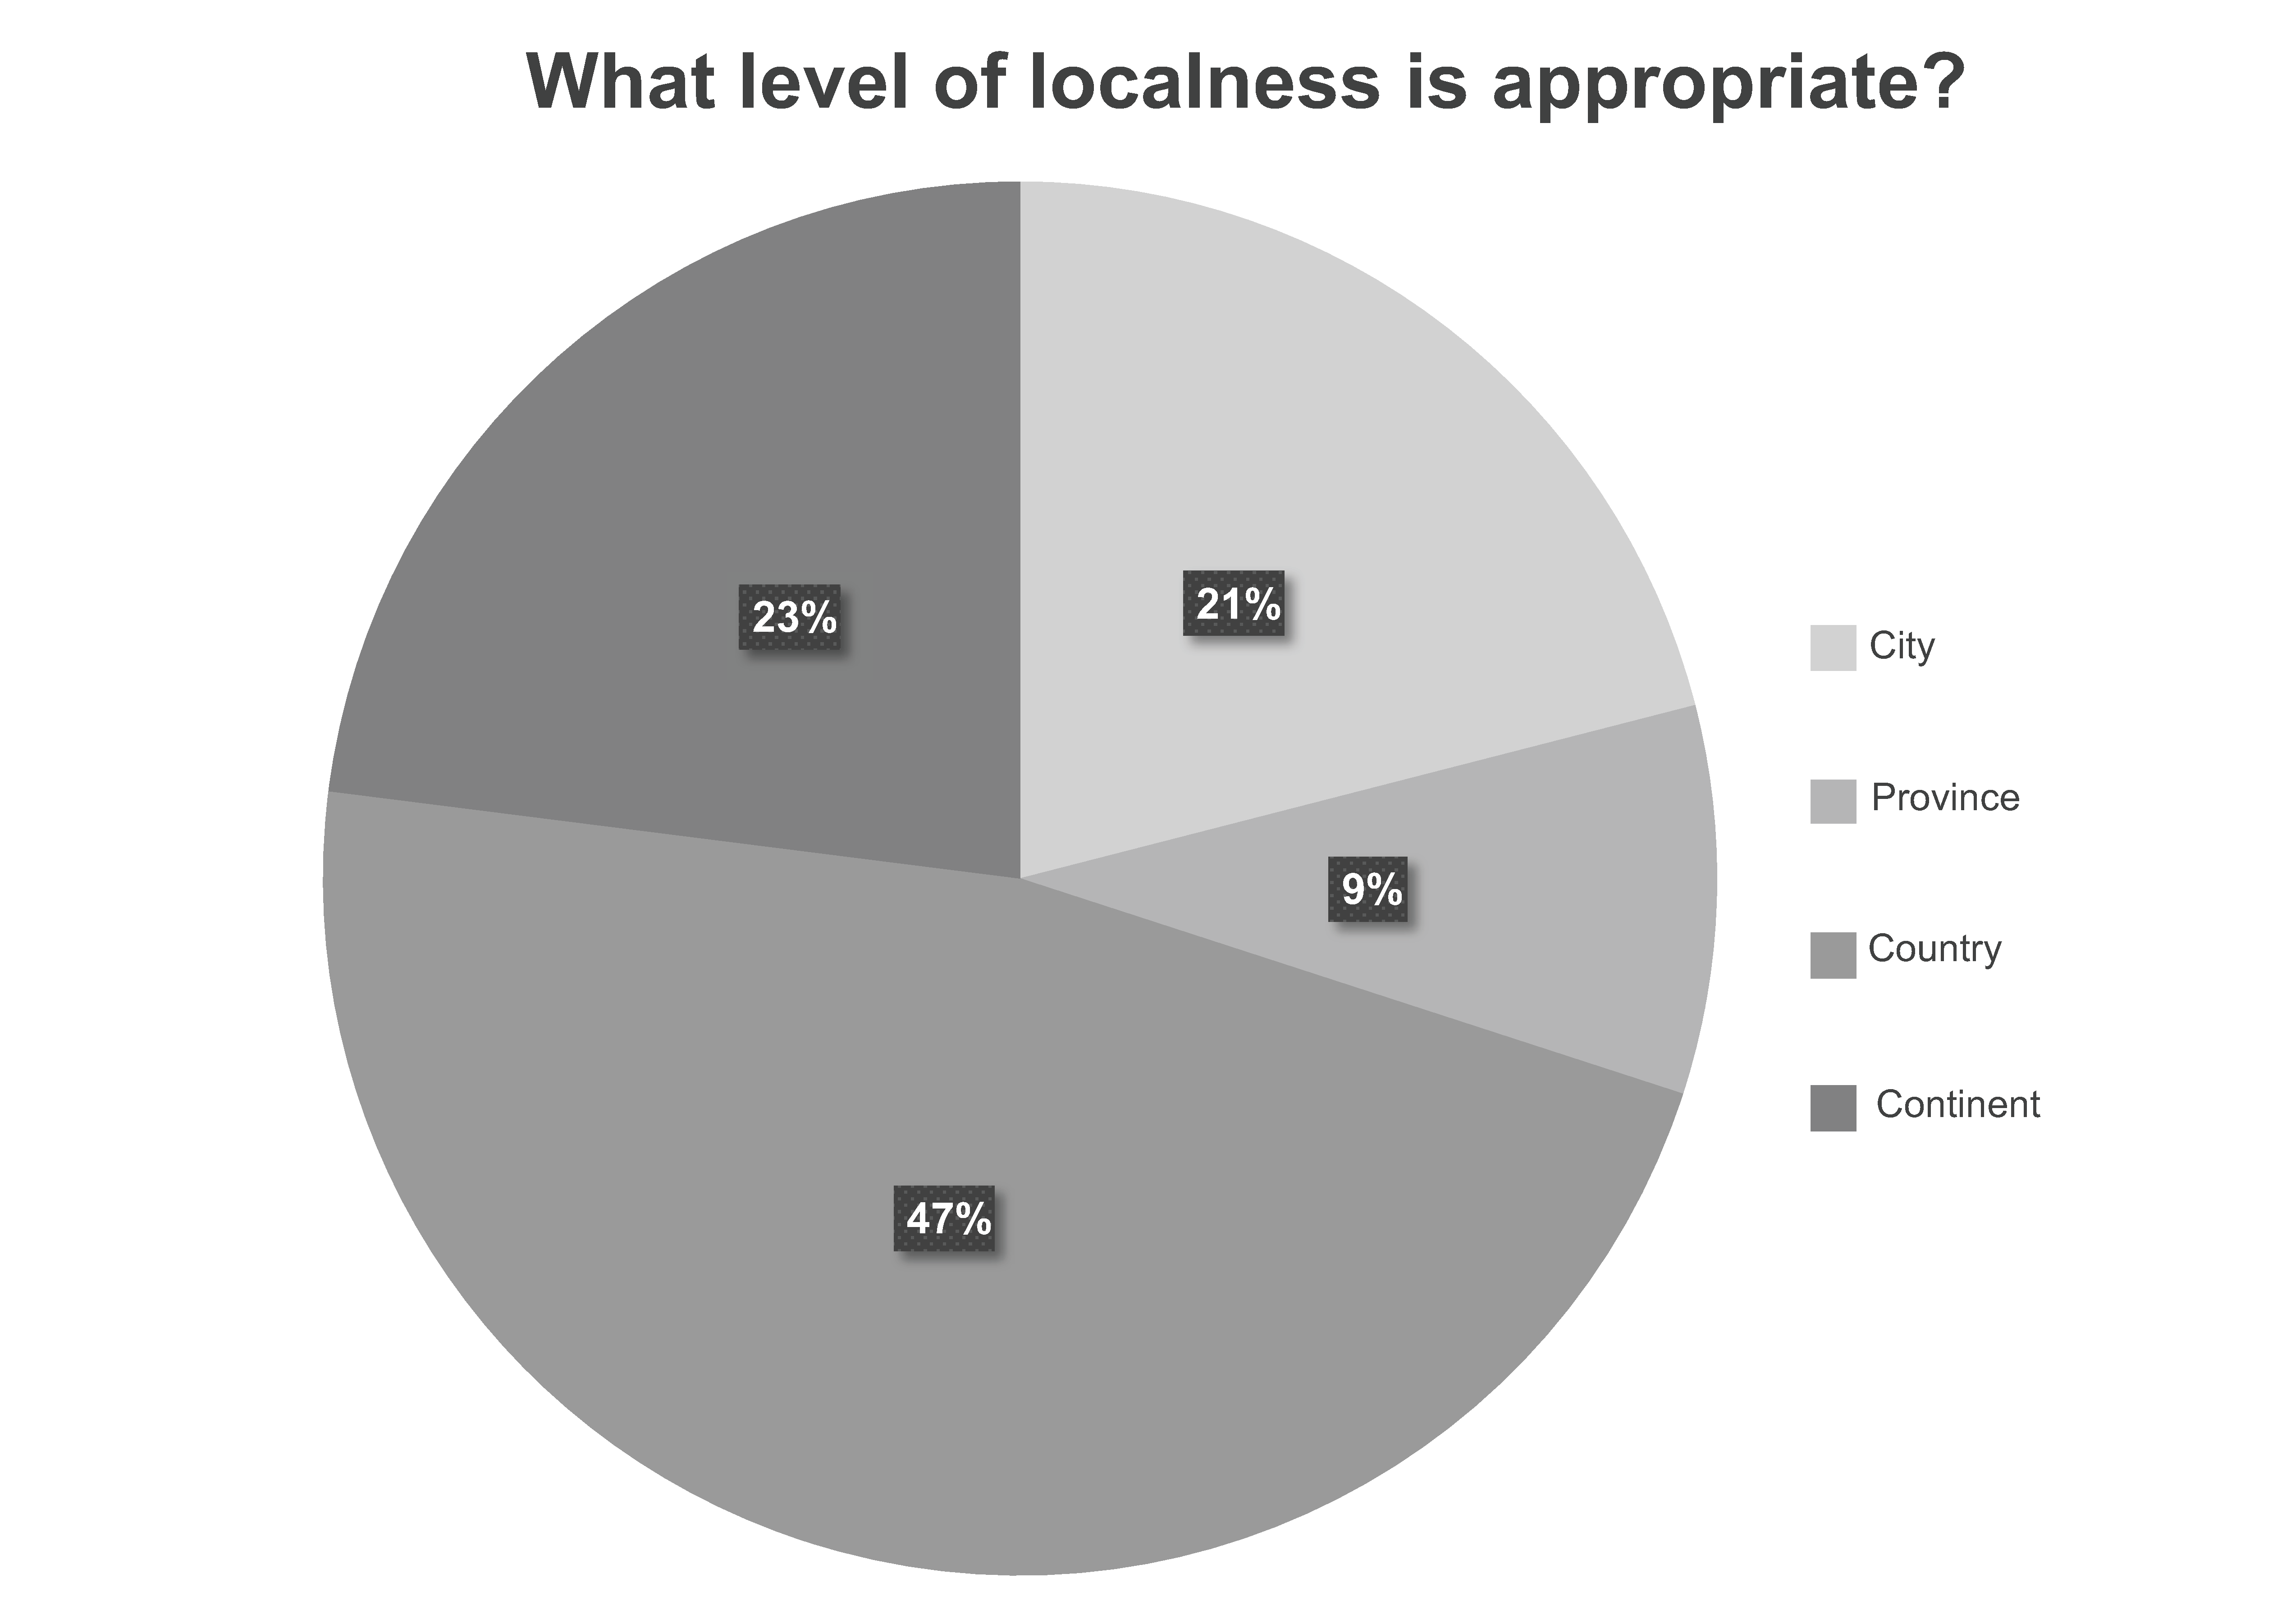
\includegraphics[width=.8\textwidth]{ART_Soloducha/illustration1.pdf}%
 \end{center}%
 \caption{Most interesting results of the survey in terms of clustering of preferences of AV users. Source: Author's study.}\label{sol-ill1}
\end{figure}
%Illustration 1

The responses are split almost equally between the preferences of the driver and the preferences of the residents of the area in which the vehicle travels, with a~slight advantage to the driver. The conclusion for manufacturers of autonomous devices is therefore that a~device should have an open architecture that allows it to be adapted to the preferred option, unless legal regulations decide otherwise. However, as the survey results show, imposing solutions in this area may end in reduced trust in the device.
\begin{figure}
 \begin{center}
 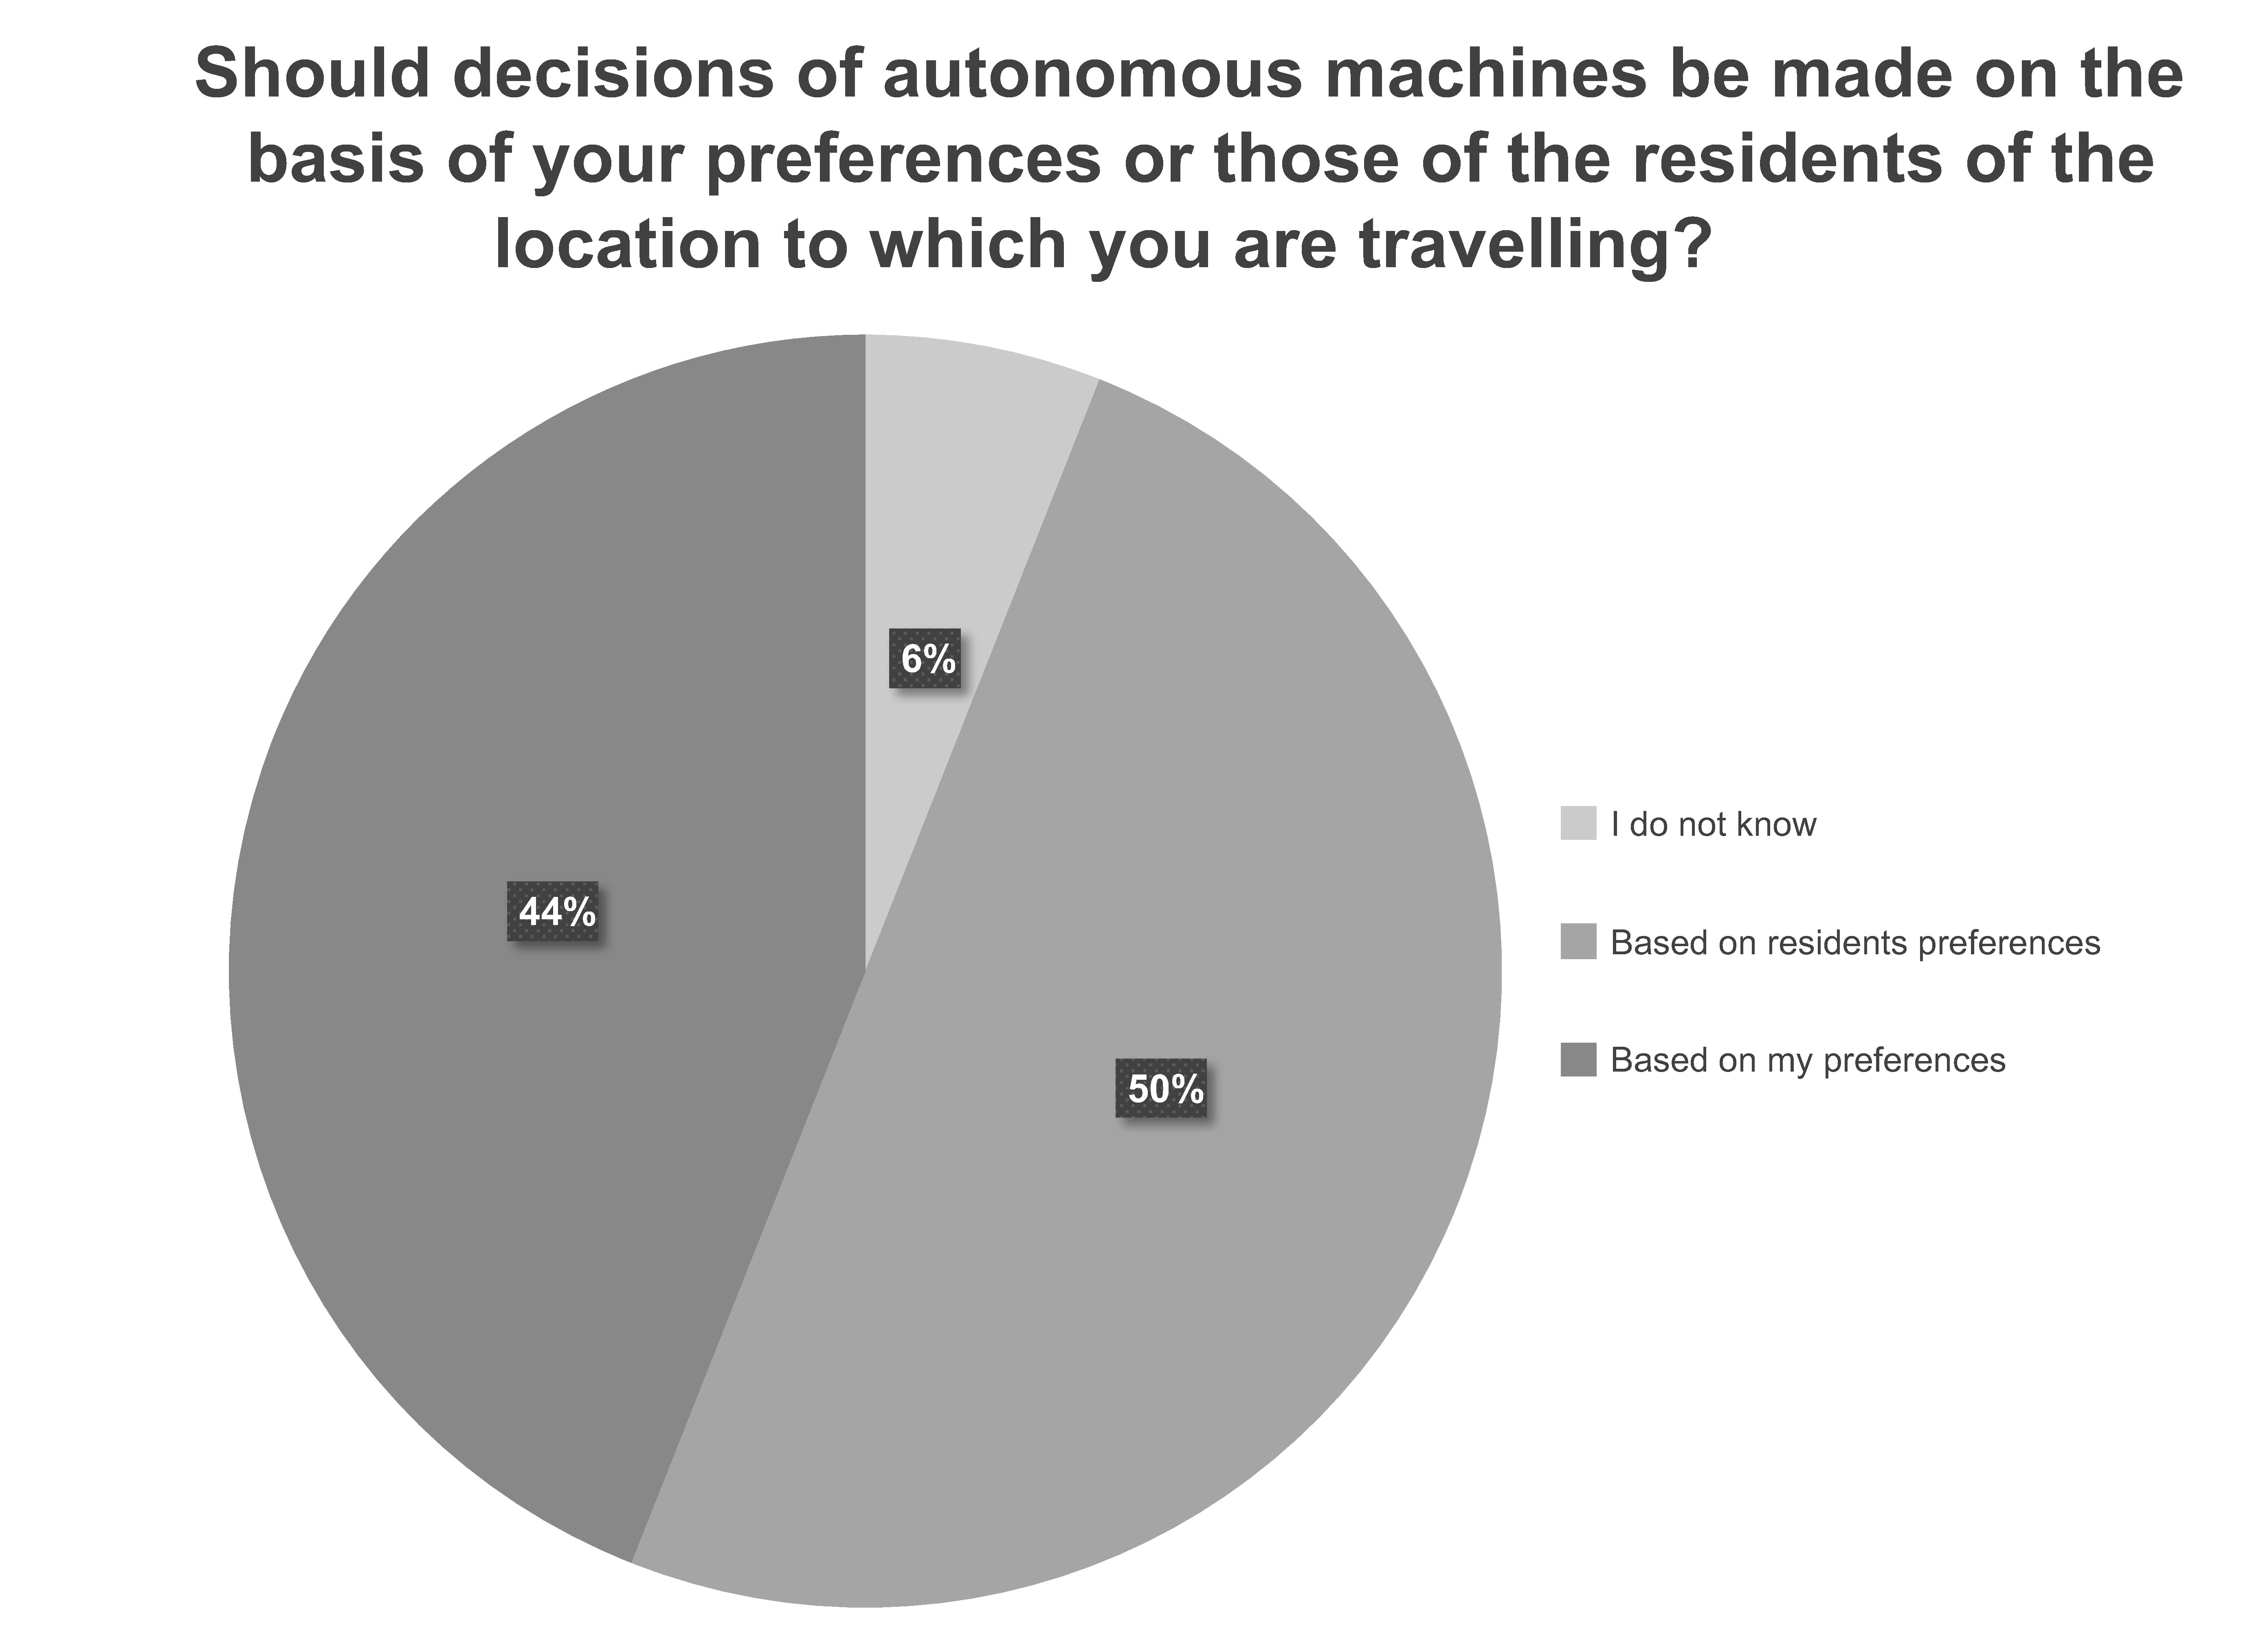
\includegraphics[width=.8\textwidth]{ART_Soloducha/illustration2.pdf}%
 \end{center}%
 \caption{Level of clustering survey. Source: Author's study.}\label{sol-ill2}
\end{figure}
%Illustration 2
%Source: Author's study

The other problem investigated in the survey was the level of clustering. The top level used in the research was the continental one. The majority of respondents preferred the level of state. The level of clustering reflecting Ingelhart-Welzel's map of cultural influences used in the research mentioned above did not appear among the questions. This does not reflect traditional geographical and administrative distinctions.

\section*{Conclusion}
Despite the sceptical voices raised against the practical implementation of the idea of an extrapolated, coherent volition of humanity in the form of the Moral Machine project, it does not seem that this criticism undermines certain important arguments that stand behind Yudkowsky's CEV project and its implementation attempts. In conclusion, we would like to point them out and outline some possible paths for further consideration of this issue.

Firstly, Yudkowsky's project and attempts to implement it are answers to the question of what moral patterns should be introduced into the decision-making procedures of machines so that they meet Giddens' active trust requirements. Any attempts to do this in a~top-down model by enlightened bodies, special committees or top-down adopted normative systems does not meet the criterion of persuasive trust proposed by Giddens. Therefore, the attempt to do this in a~descriptive way through empirical research referring to extrapolation of results of the survey seems a~method tailored to these needs, with all of the doubts associated with the naturalisation of morality and the limitations of descriptive research related to Hume's guillotine problem. Although, in our paper, we tried to show that the weak rationality associated with the inductive approach applied to moral problems can be used to overcome the is-ought problem in the case of the ethics of autonomous machines.

Secondly, such considerations can be conducted under the assumption that the best path to their implementation is to define cognitive processes (including those of a~moral nature) as consisting of information processing. What may help here may be the assumption that such a~definition of moral cognition would not be a~naturalisation
%\label{ref:RNDAVNr8uUo2k}(Rosenbloom, 2015).
\parencite[][]{peruzzi_beginners_2015}. %
 This also could help to eliminate the troubling issue of the \textit{is-ought problem}. Although it is an issue considered by some theorists to be an illusory 
%\label{ref:RNDke81GSJMB7}(Gellner, 2005)
\parencite[][]{gellner_words_2005} %
 and an argument that is treated as untenable nowadays 
%\label{ref:RNDv1WxbP4FgK}(Searle, 1964)
\parencite[][]{searle_how_1964} %
 from point of view of ``weak'' rationality—as mentioned above.

Thirdly, the acceptance of the possibility of clustering moral patterns can lead to the idea of constructing the architecture of autonomous machines as open for adaptation of the patterns used for decision-making to the local characteristics of the user/social environment. The sample survey presented at the end of the paper demonstrates the preferences of a~limited group of respondents regarding this issue.

Fourthly, there is quite advanced research on the technology of so-called social robots, whose task is to produce a~personalised interactive communication experience by considering the preferences of the user the robot interacts with
%\label{ref:RNDaTAZLD4Bt6}(Maroto-Gómez et al., 2022).
\parencite[][]{maroto-gomez_adaptive_2022}. %
 It is based on technology so called preference learning 
%\label{ref:RNDU0HNfJ31Dd}(Fürnkranz and Hüllermeier, 2011).
\parencite[][]{furnkranz_preference_2011}. %
 Using an online survey, participants provide their defining features and preferences towards the activities of the robot. Then, a~preference learning model estimates the preferences of new users using similar features of the survey participants. The survey contains questions about sociodemographic, habits, interests, and preferences about specific attributes related to social robot 
%\label{ref:RNDy6uoBMKwmA}(Fürnkranz and Hüllermeier, 2011, p.2).
\parencite[][p.2]{furnkranz_preference_2011}.%


\paragraph{Acknowledgments.}
The author wishes to thank anonymous helpful referees whose insightful comments helped improve the quality of the present paper. Most certainly, if there are still some errors remaining, they are my own responsibility.



\end{artengenv}

%\section*{References}
%Arrow, K.J., 1973. Some Ordinalist-Utilitarian Notes on Rawls's Theory of Justice. \textit{The Journal of Philosophy}, [online] 70(9), pp.245–263. https://doi.org/10.2307/2025006.
%
%Asimov, I., 2004. Runaround. In: \textit{I, robot}, Bantam spectra book, Bantam hardcover edition. New York: Bantam Books. pp.30–55.
%
%Awad, E., Dsouza, S., Shariff, A., Rahwan, I. and Bonnefon, J.-F., 2020. Universals and variations in moral decisions made in 42 countries by 70,000 participants. \textit{Proceedings of the National Academy of Sciences}, [online] 117(5), pp.2332–2337. https://doi.org/10.1073/pnas.1911517117.
%
%Bigman, Y.E. and Gray, K., 2020. Life and death decisions of autonomous vehicles. \textit{Nature}, [online] 579(7797), pp.E1–E2. https://doi.org/10.1038/s41586-020-1987-4.
%
%Bostrom, N., 2016. \textit{Superintelligence: Paths, Dangers, Strategies}. Oxford: Oxford University Press.
%
%Burrell, J., 2016. How the machine ‘thinks': Understanding opacity in machine learning algorithms. \textit{Big Data \& Society}, [online] 3(1), pp.1–12. https://doi.org/10.1177/2053951715622512.
%
%Czyżowska, D., Niemczyński, A. and Kmieć, E., 1993. Formy rozumowania moralnego Polaków w~świetle danych z~badania metodą Lawrence'a Kohlberga. \textit{Kwartalnik Polskiej Psychologii Rozwojowej}, 2(1), pp.19–38.
%
%Dignum, V., 2022. \textit{Responsible Ai: From Principles to Action}. [online] Michigan Institute for Data Science. Available at: {\textless}https://www.youtube.com/watch?v=LwKDOwwJpL4{\textgreater} [Accessed 11 January 2023].
%
%Edmonds, E., 2017. \textit{Americans Feel Unsafe Sharing the Road with Fully Self-Driving Cars}. [online] AAA Newsroom. Available at: {\textless}https://newsroom.aaa.com/2017/03/americans-feel-unsafe-sharing-road-fully-self-driving-cars/{\textgreater} [Accessed 11 January 2023].
%
%Eschenbach, W.J. von, 2021. Transparency and the Black Box Problem: Why We Do Not Trust AI. \textit{Philosophy \& Technology}, [online] 34(4), pp.1607–1622. https://doi.org/10.1007/s13347-021-00477-0.
%
%Foot, P., 2002. \textit{Virtues and Vices}. [online] Oxford University Press. https://doi.org/10.1093/0199252866.001.0001.
%
%Fukuyama, F., 1995. \textit{Trust: the social virtues and the creation of prosperity}. 1st ed. A~Free Press paperbacks book. New York: Free Press.
%
%Fürnkranz, J. and Hüllermeier, E., 2011. Preference Learning: An Introduction. In: J. Fürnkranz and E. Hüllermeier, eds. \textit{Preference Learning}. [online] Berlin, Heidelberg: Springer. pp.1–17. https://doi.org/10.1007/978-3-642-14125-6\_1.
%
%Gellner, E., 2005. \textit{Words and Things: An Examination of, and an Attack on, Linguistic Philosophy}. 1. publ ed. Routledge classics. London: Routledge.
%
%Giddens, A., 1991. \textit{Modernity and Self-Identity: Self and Society in the Late Modern Age}. Stanford, CA: Stanford University Press.
%
%Górnicka, J., 1980. Rozwój moralny w~koncepcji Lawrence'a Kohlberga. \textit{Człowiek i~Światopogląd}, 6, pp.113–123.
%
%Greene, J.D., 2013. \textit{Moral Tribes: Emotion, Reason, and the Gap Between Us and Them}. London: Atlantic Books.
%
%Gryz, J., 2021. \textit{Sztuczna~Inteligencja:~powstanie,~rozwój,~rokowania}. [online] Copernicus Center. Available at: {\textless}https://www.youtube.com/watch?v=3ZDfVgC897k{\textgreater} [Accessed 11 January 2023].
%
%Harsanyi, J.C., 1975. Can the Maximin Principle Serve as a~Basis for Morality? A~Critique of John Rawls's Theory. \textit{The American Political Science Review}, [online] 69(2), pp.594–606. https://doi.org/10.2307/1959090.
%
%Hofstede, G.H., Hofstede, G.J. and Minkov, M., 2010. \textit{Cultures and Organizations: Software of the Mind: Intercultural Cooperation and Its Importance for Survival}. 3rd ed ed. New York: McGraw-Hill.
%
%Hofstede, G.J., 2011. \textit{Geert Hofstede on Culture}. [online] Viewdutch. Available at: {\textless}https://www.youtube.com/watch?v=wdh40kgyYOY{\textgreater} [Accessed 11 January 2023].
%
%Holstein, T. and Dodig-Crnkovic, G., 2018. Avoiding the intrinsic unfairness of the trolley problem. In: \textit{Proceedings of the International Workshop on Software Fairness}. [online] ICSE '18: 40th International Conference on Software Engineering. Gothenburg Sweden: ACM. pp.32–37. https://doi.org/10.1145/3194770.3194772.
%
%Inglehart, R. and Welzel, C., 2005. \textit{Modernization, Cultural Change, and Democracy: The Human Development Sequence}. [online] Cambridge: Cambridge University Press. https://doi.org/10.1017/CBO9780511790881.
%
%Jörgensen, J., 1937. Imperatives and logic. \textit{Erkenntnis}, [online] 7(1), pp.288–296. https://doi.org/10.1007/BF00666538.
%
%Karpus, J., Krüger, A., Verba, J.T., Bahrami, B. and Deroy, O., 2021. Algorithm exploitation: Humans are keen to exploit benevolent AI. \textit{iScience}, [online] 24(6), p.102679. https://doi.org/10.1016/j.isci.2021.102679.
%
%Kohlberg, L., 1958. \textit{The Development of Modes of Moral Thinking and Choice in the Years 10 to 16}. [PhD thesis] University of Chicago. Available at: {\textless}https://www.proquest.com/openview/c503bf59d762abe5818e1b24c484d41a/1?pq-origsite=gscholar\&cbl=18750\&diss=y{\textgreater} [Accessed 11 January 2023].
%
%Lo, T., 2019. \textit{My Amazon Alexa Went Rogue and Ordered Me to Stab Myself in the Heart}. [online] Mirror Online. Available at: {\textless}https://www.mirror.co.uk/news/uk-news/my-amazon-echo-went-rogue-21127994{\textgreater} [Accessed 11 January 2023].
%
%Maroto-Gómez, M., Castro-González, Á., Castillo, J.C., Malfaz, M. and Salichs, M.Á., 2022. An adaptive decision-making system supported on user preference predictions for human–robot interactive communication. \textit{User Modeling and User-Adapted Interaction}, [online] pp.1–45. https://doi.org/10.1007/s11257-022-09321-2.
%
%Miłaszewicz, D., 2016. Zaufanie jako wartość społeczna. \textit{Studia Ekonomiczne}, [online] (259), pp.80–88. Available at: {\textless}http://cejsh.icm.edu.pl/cejsh/element/bwmeta1.element.cejsh-d64b921a-5db7-4208-9eb7-73baaa05f7e4{\textgreater} [Accessed 11 January 2023].
%
%Mirnig, A.G. and Meschtscherjakov, A., 2019. Trolled by the Trolley Problem: On What Matters for Ethical Decision Making in Automated Vehicles. In: \textit{Proceedings of the 2019 CHI Conference on Human Factors in Computing Systems}. [online] CHI '19: CHI Conference on Human Factors in Computing Systems. Glasgow Scotland Uk: ACM. pp.1–10. https://doi.org/10.1145/3290605.3300739.
%
%Nagel, T., 1986. \textit{The View from Nowhere}. 1st ed. Oxford: Oxford University Press.
%
%Nozick, R., 2013. \textit{Anarchy, State, and Utopia}. New York: Basic Books.
%
%Pasquale, F., 2016. \textit{The Black Box Society: The Secret Algorithms That Control Money and Information}. Cambridge, MA: Harvard University Press.
%
%Rawls, J., 1971. \textit{A~Theory of Justice}. [online] Cambridge, MA: The Belknap Press of Harvard University Press. Available at: {\textless}http://www.gbv.de/dms/bowker/toc/9780674880146.pdf{\textgreater} [Accessed 11 January 2023].
%
%Rosenbloom, P., 2015. \textit{On Computing: The Fourth Great Scientific Domain}. Cambridge, MA: The MIT Press.
%
%Searle, J.R., 1964. How to Derive ‘Ought' From ‘Is'. \textit{The Philosophical Review}, [online] 73(1), pp.43–58. https://doi.org/10.2307/2183201.
%
%Wysocki, I., 2021. The problem of indifference and homogeneity in Austrian economics: Nozick's challenge revisited. \textit{Philosophical Problems in Science (Zagadnienia Filozoficzne w~Nauce}), [online] (71), pp.9–44. Available at: {\textless}https://zfn.edu.pl/index.php/zfn/article/view/554{\textgreater} [Accessed 24 January 2022].
%
%Yudkowsky, E., 2004. \textit{Coherent Extrapolated Volition}. San Francisco, CA: San Francisco.
%\end{document}

%\begin{artengenv2auth}{Alice Martin, Mathieu Magnaudet, Stéphane Conversy}
	{Modelling interactive computing systems: Do we have a~good theory of what computers are?}
	{Modelling interactive computing systems\ldots}
	{Modelling interactive computing systems: Do we have a~good theory\\of what computers are?}
	{\textsuperscript{1}Departments of Philosophy and Mathematics, Carnegie Mellon University\\
		\textsuperscript{2}Copernicus Center for Interdisciplinary Studies, Jagiellonian University}
	{Computers are increasingly interactive. They are no more transformational systems producing a~final output after a~finite execution. Instead, they continuously react in time to external events that modify the course of computing execution. While philosophers have been interested in conceptualizing computers for a~long time, they seem to have paid little attention to the specificities of interactive computing. We propose to tackle this issue by surveying the literature in theoretical computer science, where one can find explicit proposals for a~model of interactive computing. 
	In that field, the formal modelling of interactive computing systems has been brought down to whether the new interaction models are reducible to Turing Machines. There are three areas where interaction models are framed. The comparison between TMs and interactive system models is at stake in all of them. These areas are namely some works on concurrency by Milner, on Reactive Turing Machines, and on interaction as a~new computing paradigm. For each of the three identified models, we present its motivation, sum up its account for interaction and its legacy, and point out issues regarding the understanding of computers. The survey shows difficulties for epistemologists. The reason is that these analyses focus on the formal equivalence between interactive models of computation and classic ones. Such a~project is different from addressing how a~computing machine can be interactive: in other words, which mechanisms allow it.}
	{philosophy of computing, models of computation, interactive computing, computing mechanism, computational mechanistic explanation.}
	{%
%		{\flushright\subbold{Alice Martin}\\\subsubsectit\small{ENAC, Université de Toulouse}\par}%
%		{\flushright\subbold{Mathieu Magnaudet}\\\subsubsectit\small{ENAC, Université de Toulouse}\par}%
%		{\flushright\subbold{Stéphane Conversy}\\\subsubsectit\small{ENAC, Université de Toulouse}\par}%
				{\flushright\subbold{Alice Martin}\\\subbold{Mathieu Magnaudet}\\\subbold{Stéphane Conversy}\\
				\subsubsectit\small{ENAC, Université de Toulouse, France}\par}%
	}

%\documentclass[a4paper, 11pt, twoside]{article}
%
%%Citation-related commands
%%PP\usepackage{natbib}
%%PP\setcitestyle{authoryear,open={(},close={)}} 
%%PP \bibliographystyle{agsm}
%
%\usepackage[utf8]{inputenc}
%\usepackage{hyperref}
%%PP \renewcommand\harvardyearleft{\unskip, }
%%PP \renewcommand\harvardyearright[1]{.}
%%PP \hypersetup{hidelinks}
%
%\usepackage[top=3cm, bottom=3cm, left=3cm, right=3cm]{geometry}
%%\usepackage{amsmath}
%%\usepackage{amssymb}
%%\usepackage{mathrsfs}
%\usepackage{lmodern}
%%\usepackage[latin1]{inputenc}
%\usepackage[T1]{fontenc}
%\usepackage{dsfont}
%\usepackage{listings}
%\usepackage[table]{xcolor}
%%\usepackage{mathrsfs}
%\usepackage{float}
%\usepackage[justification = centering]{caption}
%%\usepackage{amsmath}
%\usepackage{graphicx}
%%\usepackage{lmodern}
%%\usepackage{bm} 
%
%%PP added
%\usepackage[style=bath, citestyle=authoryear-comp, backend=biber]{biblatex} %uwaga: wymaga zmiany procesora bibliografii na biber
%\addbibresource{Martin.bib}
%%end of PP added
%
%
%\title{Modelling Interactive Computing Systems: Do We Have a~Good Theory of What Computers Are?}
%%\date{}
%\author{Alice Martin, Mathieu Magnaudet, Stéphane Conversy}
%
%\begin{document}
%
%\maketitle
%
%Computers are increasingly interactive. They are no more transformational systems producing a~final output after a~finite execution. Instead, they continuously react in time to external events that modify the course of computing execution. While philosophers have been interested in conceptualizing computers for a~long time, they seem to have paid little attention to the specificities of interactive computing. We propose to tackle this issue by surveying the literature in theoretical computer science, where one can find explicit proposals for a~model of interactive computing. 
%In that field, the formal modelling of interactive computing systems has been brought down to whether the new interaction models are reducible to Turing Machines. There are three areas where interaction models are framed. The comparison between TMs and interactive system models is at stake in all of them. These areas are namely some works on concurrency by Milner, on Reactive Turing Machines, and on interaction as a~new computing paradigm. For each of the three identified models, we present its motivation, sum up its account for interaction and its legacy, and point out issues regarding the understanding of computers. The survey shows difficulties for epistemologists. The reason is that these analyses focus on the formal equivalence between interactive models of computation and classic ones. Such a~project is different from addressing how a~computing machine can be interactive: in other words, which mechanisms allow it. \\
%
%
%Keywords: philosophy of computing, models of computation, interactive computing, computing mechanism, computational mechanistic explanation


%\renewcommand{\thesection}{.\arabic{section}}
\section*{Introduction}

\lettrine[loversize=0.13,lines=2,lraise=-0.03,nindent=0em,findent=0.2pt]%
{I}{}n the philosophy of computing, we are paying increased attention to a~set of new features of computers. This set has led to the introduction of a~new label for these computing machines: they are referred to as interactive computing machines \parencite{Dodig-Crnkovic2011, Goldin2006, Soare2013, VanLeeuwen2001, Wegner1997}. The set of new features can be captured in the following statement made in a~2011 paper by Gordana Dodig-Crnkovic (our highlights): 

\myquote{
 Present day computers are very different from the early stand-alone calculators designed for mechanizing mathematical operations. They are largely \emph{used for communication in world-wide networks} and variety of information processing and knowledge management. Moreover, they play \emph{an important role in the control of physical processes and thus connect to the physical world}, especially in automation and robotics. [\ldots] Computational processes are nowadays \emph{distributed, reactive, agent-based, and concurrent}. The main criterion of success of the computation is not its termination, but its \emph{response to the outside world}, its speed, generality and flexibility; adaptability, and tolerance to noise, error, faults, and damage \parencite{Dodig-Crnkovic2011}.
 }

Historically, the concept of interaction was introduced by a~computer scientist, Milner, in the 1970s-1980s \parencite{Milner1975, Milner1982, Milner1993, Milner1999}. At first, an \emph{interactive computing system} was defined as a~system where several threads execute instructions in parallel while being able to synchronize and communicate at certain moments of the execution. Since then, the characteristics of computer systems have continued to evolve, and by ``interactive'' we refer today to a~broader set of properties that can be grouped as follows: the ability to continuously react in time to external events that modify computing execution. 
This class of computers deserves all our attention since they are ubiquitous. Every computer system today is designed to respond to external events in a~predictable way and according to temporal constraints. In any case, what distinguishes this class of so-called interactive computing machines from the classical computer systems that preceded them is that they are no longer purely \emph{transformational systems}. A~\emph{transformational system} is a~classical computing device that, given a~set of inputs, produces a~final output after a~finite execution. 
This evolution of computing complicates the answer to \textit{what a~computer is}. The question is well-known in the philosophy of computing \parencite{Piccinini2008, Rapaport2018, Smith2002}. As already noted, many answers to the question distort it and answer the question of \textit{what a~computation is}, immediately projecting the field of investigation into the theory of computability: 


\myquote{
A~fairly obvious, trivial, and almost-circular definition of ‘computer’ says that a~computer is a~machine that computes. The natural next question is: What does it mean to compute? But this shifts the burden of answering our question away from what computers are to the topic of what computation is. Many of the objections to various theories about computers are really objections to what counts as a~computation \parencite{Rapaport2018}. 
}

This leaves us with the specific issue we want to address. We ask whether models of computation for interaction allow us to answer the question of what an actual (necessarily interactive) computer is. Current computers come in various forms and we chose in this paper to restrict our concerns to a~delimited notion of \textit{interaction}, as defined in Human-Computer Interaction \parencite{Myers1994, Dearden1997, Beaudouin-Lafon2006,  Hornbaek2017, Basman2018}, and target a~specific set of ubiquitous computing devices---those interacting with humans, e.g., through digital interfaces. We will not elaborate on \textit{analog computing} \parencite{Bielecki2019} and \textit{natural computation} \parencite{Dodig-Crnkovic2011, MacLennan2003}. 

To tackle the issue of interactive computing devices, we propose here an approach that, to the best of our knowledge, has not been proposed so far: we want to examine the models of computation proposed in theoretical computer science to think about interactive computing systems. We offer a~literature survey where one can find \textit{explicit theories of interaction}.\footnote{We insist on our two criteria: \textit{explicit theories of interaction} in \textit{theoretical computer science}. We have in mind the fact that other communities e.g., the engineering community on reactive systems, are related to our topic but they have not conceptualized \textit{interaction} as such.} We show that the formal modelling of interactive computing systems has been brought down to whether the new interaction models are reducible to Turing’s \emph{a-machines} \parencite{Turing1937}---we will refer to them as Turing Machines (TMs). 
Questioning the theoretical bounds of the Turing Machine in computer science when faced with the existence of interactive computing devices has been explored at least since Milner's work on communicating and mobile systems \parencite{Milner1993, Milner1999}. To the best of our knowledge, there are three areas where interaction models are framed as such. These areas are some works (i) on concurrency by Milner and his followers \parencite{Milner1999, Milner2006}, (ii) on Reactive Turing Machines \parencite{Andersen1997, Baeten2013, VanLeeuwen2001, VanLeeuwen2006}, and (iii) on interaction as a~new non-algorithmic computing paradigm \parencite{Goldin2006, Wegner1997, Wegner2003}. For each of the three identified models, we:

\begin{itemize}
    \item present the motivation behind it, 
    \item sum up its account for interaction,
    \item identify its legacy,
    \item point out issues regarding the understanding of computers qua that model.
\end{itemize}

We then want to show how these approaches, which belong to a~formal approach, cannot provide an answer to the question of what computers are, and for two reasons. On the one hand, these models of computation have focused their attention on whether interactive models are reducible to models of classical computation---par excellence, the Turing machine. Proving (or not) that an interactive property can be formalized as a~computable property in the classical Turing’s sense does not answer the question of how an interactive property comes into existence and can be the object of execution. On the other hand, and this is a~correlate, these models do not propose a~basis for a~mechanistic explanation of the very possibility of an interactive computing system. With only formal models of interactive computation, we might run the risk of not offering an adequate conceptualization of current computers. Therefore, we end up proposing to take the distinction seriously between \emph{models of computation} and \emph{mechanistic computational explanations}, as presented by Miłkowski \parencite*{Mikowski2011, Mikowski2014}.

\section{Milner introduces a~distinction between interactional and computational behavior}
\label{Milner}
%\vskip -2\baselineskip
\subsection{Motivation}

Milner was the one who introduced the concept of interaction in computer science. He summarized his motivations in a~famous Turing Award speech \parencite{Milner1993}. Milner was concerned with the logical foundations of computing inherited from Turing. He was preoccupied with the idea that computing practices had evolved since the birth of computing, notably in terms of architecture. He took seriously the possibility that the logical foundations dating back to the thirties may not match the growing challenges of his time and may require additional concepts.

Milner \parencite*{Milner2006} pointed out  that the logical foundations of computing offered by Turing \parencite*{Turing1937} were previous to the first physical computers and that computer science is grounded in \emph{logic} and \emph{engineering}. On the engineering side, computer science was inherited from von Neumann’s pioneering work \parencite{Godfrey1993, Aspray1990}. Only one thing could happen at once in an early von Neumann's computer. Nevertheless, there was more to computing than von Neumann's architecture \parencite{Backus1978, Milner2006}. A~growing interest in dealing with concurrency in the sixties and seventies made sequential programming less warranted. Therefore, to Milner, the logical foundations of computing were to evolve. The main flaw of the early logical foundations was the reduction of computing processes to the concept of an algorithm, which tends to associate computing with mere calculation without taking concurrent activity into account. Because of the evolution of computing engineering practice, Milner questioned whether the logical grounds of computing should evolve as well. Milner's thesis can be put in a~nutshell: ``this logical foundation has changed a~lot since Turing but harks back to him. To be more precise: (i) Computing has grown into informatics---the science of interactive systems; (ii) Thesis: Turing's logical computing machines are matched by a~logic of interaction'' \parencite{Milner2006}. Consequently, a~theory and new language to express concurrent activity were required: ``we must find an elementary model which does for interaction what Turing's logical machines do for computation'' \parencite{Milner2006}. 

The need to define a~new computing theory is first displayed through the evolution of computing practice.
To sum up, Milner’s motivation and focus were the solving of concurrency issues in distributed systems, with the idea that the evolution of computing practices required new formal tools: ``Through the 1970s, I~became convinced that a~theory of concurrency and interaction requires a~new conceptual framework, not just a~refinement of what we find natural for sequential [algorithmic] computing'' \parencite{Milner1993}. 

\subsection{Account for interaction}

Milner introduced the opposition between \textit{interactional} and \textit{computational} behaviour. Introducing the concept of interaction, Milner \parencite*{Milner1975, Milner1982, Milner1983} referred to concurrent message passing between agents. Milner's work coincided with Petri’s \parencite*{Petri1980} new model of concurrent processes, which generally intended to describe concurrency in information systems.\footnote{Concurrency theory emerged from Dick Karp's early work in the 1960s, grew with \parencite{Petri1980} and later work on transition systems \parencite{Nielsen1981, Glabbeek2004},
and has now developed into a~mature theory of reactive systems \parencite{Harel1985} with diverse network models \parencites[for an overview, see][]{Lee1998}{Lee2006_modelsofcomputation}.}
 To Milner, interaction is more \textit{expressive} than a~TM, but it still describes an \textit{effective} procedure. Milner did not assert \textit{equivalence} between an interactive model and a~TM, but he introduced the topic \parencite{Milner1999} and left it unanswered. 
Four main differences between old (computational) and new (interactional) computing are made striking by Milner. First, in Milner’s words, a~Turing Machine prescribes a~behaviour to be executed. In contrast, new computing requires the description of an information flow between several system components. Second, old computing is characterized by a~\textit{hierarchical design} when current practice involves \textit{heterarchical} phenomena in the computing system. Third, in new computing, the designer cannot predict when agents will be triggered or the overall behaviour of the computing system. Fourth, the user is not merely looking for an end result in new computing practice. There is more than a~mathematical function to evaluate, as it used to be in old computing. The user instead interacts with the system, and the look for an end result is replaced by continuing interaction. Having taken stock of the evolution of computing practice on the engineering side, Milner examines its consequences on the logic foundations of computing. The pi-calculus and his work on the equivalence with automata, known as bisimulation, achieved this reflection on interactive processes \parencite{Milner1993, Milner1999} with a~formalism.

\subsection{Legacy}

Milner's work on interaction has become a~founding block in automata theory and concurrency theory. It installed the notion of a~transition system as the prime mathematical model to represent discrete behavior \parencite{Nielsen1981, Baldan2001, Glabbeek2004, Arbach2015}. It also showed that language equivalence was not the correct notion when comparing automata for interactive systems.
Instead, it should be replaced by a~notion of behavioral equivalence or bisimilarity~\parencite{Milner1999}. The pi-calculus has inspired research to derive a~language from it. The \textit{Pict} \parencite{Pierce2000} programming language is an example. 

Milner's work is foundational and served as a~reference for anyone after him, reflecting on the need for a~new framework dedicated to new emerging computing practices. Milner insists on an essential reminder that we would like to consider. When modelling, the engineering practice matters and is to be articulated with the logical foundations of the model, should it involve elaborating a~new framework. Famously, Wegner and Goldin acknowledge that Milner was the first to introduce the idea that classic models of computation were insufficient. They argue that Milner did not state clearly whether computation in concurrent communicating systems (CCS) and the pi-calculus were reducible to Turing machines and algorithms \parencite{Wegner2003}. If one goes and looks at Milner’s Turing Award Speech, it seems true that classical computation translates into an interactive calculus. However, it is not stated whether any formula in the pi-calculus can be expressed in a~classical calculus like the lambda-calculus.

\subsection{Issues for an account of current computers}

Given the account of current computers that we are looking for, we see two limits in the lessons drawn from Milner.
First, we are looking for an explanation of the interactive computing phenomena at stake in a~computer. Therefore, the relation between layers of abstraction, from the computational to the physical, is crucial. However, to Milner, the physical layer of the machine is not of much interest, and the calculus of CCS needs to abstract away from the physical. As Milner puts it, informatics is about virtual symbols: ``physical systems tend to have permanent physical links; they have fixed structure. But most systems in the informatic world are not physical; their links may be virtual or symbolic'' \parencite{Milner1999}. From our perspective, abstracting away from the physical world comes at some cost for an explanation. A~complete explanation of a~computing system can hardly be provided in details within a~single understandable abstraction, since a~computing sytems is extremely  multi-layered~\parencite{Nisan2005, Plato2018}. Therefore, an explanation of a~computing system is necessarily a~trade-off between understandability and overwhelming details. As we will flesh out in the last section \ref{debate} by referring to Miłkowski’s work \parencite{Mikowski2011, Mikowski2016}, a~good computational explanation must link the formal story and the blueprint of the computing mechanism. Such articulation is not told in a~formal theory of concurrent processes. 
Second, this first story of interactive systems restricts them to concurrent systems, which is only one dimension of interest when describing what current computers do. There are \textit{at least} two core dimensions left aside: what makes possible timing instructions and the connection between physical processes inside and outside the computing system.

\section{Reactive TMs: extending the original model}
\label{RTMS}
%\vskip -2\baselineskip
\subsection{Motivation}

More recently, a~literature domain focused on a~``Reactive Turing machine'' has emerged 
\parencite{Andersen1997, Baeten2012, Baeten2013, Luttik2016, VanLeeuwen2006}. It reminds us that the purpose of Turing's \textit{a-machine} model was to propose a~formal account of what is \textit{computable by effective means} (algorithmically computable). This formalization was achieved before the realization of the first digital computers. In a~way reminiscent of Milner, the question is whether the TM model still fits computing practices decades later. The strategy chosen is to see whether \textit{extensions} of the original TM are sufficient to describe new computing practices and whether the obtained model is still equivalent to a~TM. The strategy founds its frame within computability theory and reflects on its scope.
This literature domain that proposes extensions of the Turing machine to account for interactive computing systems may be traced back to seminal works on a~``Universal reactive machine'' \parencite{Andersen1997}. In that respect, although pointing at the specificity of interactional behaviour, the main framework still relates to Turing's. Baeten, Luttik, and van Tilburg \parencite{Baeten2013} are looking for a~ model of interactive computation, extending the classical TM with a~process-theoretical notion of interaction related to Milner's previous work. 
The strategy involves questioning the relationship between such extensions and the Church-Turing thesis. As a~reminder, the Church-Turing thesis states that a~computable function by effective means is computable by a~Turing machine. The community interested in Reactive Turing machines asks the following question: can the Church-Turing thesis also be extended? Van Leeuwen and Wiedermann \parencite*{VanLeeuwen2001} focus on the possible extension of the Church-Turing thesis to account for interactive computing: ``We will motivate the need for a~reconsideration of the classical Turing machine paradigm and formulate an extension of the Church-Turing thesis'' \parencite{VanLeeuwen2001}. 

What is at stake is whether the Church-Turing thesis holds given warranted new models of computation: ``Is the Church-Turing thesis as we know it still applicable to the novel ways in which computers are now used in modern information technology? Will it hold for the emerging computing systems of the future?'' \parencite{VanLeeuwen2001}. 
The Church-Turing thesis originally did not entail a~claim about computing in general (what computers do and will do) but only about \textit{effective computation}. Therefore, it does not follow that we should ask the Church-Turing thesis for answers on what computing is. Replacing a~question about computing with a~question about computation is the mark of a~specific formal perspective within the frame of computability theory. Understanding \textit{computing} and its evolution from a~formal perspective consist of questioning \textit{what can be computed} and seeing if there is another notion of computation than effective computation \textit{in the sense of Church-Turing}. 

\subsection{Account for interaction}

The starting point in the Reactive TM community is a~standard current computer designed as a~distributed system interacting with an environmental agent: a~\textit{site machine}. Starting from this model, the reflection on interaction aims at showing the equivalence between this site machine and a~Turing machine augmented by some functions. The conclusion is that a~site machine computer computes effectively and yet requires a~TM with new functions, thus requiring an extension of Church-Turing's thesis. There are effectively computable functions that TMs, in a~strict sense, cannot compute. One crucial dimension that the community wants to account for is particularly relevant to us: ``In order to mimic site machines, a~Turing machine must have a~mechanism that will enable it to model the change of hardware or software by an operating agent'' \parencite{VanLeeuwen2001}. To make interaction with an external agent possible, the model needs to integrate a~way of entering new, external, and possibly non-computable information into the machine. This is precisely what oracles do. The authors prefer a~more general notion: an \textit{advice function}. The model of a~Reactive TM (also called a~TM with advice) is considered expressive and definitionally equivalent to an Oracle Turing Machine.	

Van Leeuwen and Wiedermann identify three key elements that should be integrated all together within the frame of algorithmic computability: ``non-uniformity of programs'', ``interaction of machines'', and ``infinity of operation''. By the non-uniformity of programs, the authors refer to the fact that current programs on a~personal computer are no longer fixed but evolve, are upgraded, and their data remain in memory even when the machine is not running. By interaction, they intend to contrast a~TM, where all input data are present before the start of the computing procedure, with a~modern computer, where continuous streaming of data via input ports is going on. The third mentioned characteristic, the infinity of operation, refers to distributed and mobile communication systems. These systems are to be seen as dynamic networks of many entities sending and receiving signals in unpredictable ways that are to be synchronized. To accommodate the original TM model, Leeuwen and Wiedermann propose to define ``Interactive Turing machines with advice.'' Integrating an ``advice'' function amounts to entering new, external, and non-computable information into the machine, which requires using oracles \parencite{Balcazar1995, Rogers1987}. 
This way, a~TM with advice resembles site machines and I/O automata in being equipped with input and output ports. To the authors, formal tools to support interaction and infinite computations are already available. As for interaction, they refer to already well-known and developed literature on the theory of concurrent processes, the programming of parallel processes, communication protocols, and distributed algorithms. As for infinite computations, Leeuwen and Wiedermann understand them from the language-theoretic viewpoint in the theory of omega-automata \parencite{Staiger1997, Thomas1990}.

\subsection{Legacy}

This approach to extending the Turing machine and the Church-Turing thesis is at the junction between Milner's work and Wegner's (presented in the coming section \ref{Wegner}). It makes the junction in that it begs the question of a~new paradigm. Milner had not formulated his theory of interaction in such radical terms, but Wegner goes further. The Reactive Turing Machine community asks whether the mentioned required extensions lead to a~new computing paradigm: ``The experience with present-day computing confronts us with phenomena that are not captured in the scenario of classical Turing machines'' \parencite{VanLeeuwen2001}. The computations carried out on Turing machines with advice are said to be ``more powerful'' than classic computations on a-machines. The authors insist that this claim does not go against the Church-Turing thesis. To Leeuwen and Wiedermann, like other physical systems \parencite{Pour-El1999}, TMs with advice or oracle Turing machines do not fit the concept of a~finite algorithm that can be computed by means of a~TM. The conclusion pushes towards a~paradigm shift: 

\myquote{
What makes them non-fitting under the traditional notion of algorithms is their potentially endless evolution in time. This includes both interaction and non-uniformity aspects. This gives them the necessary infinite non-uniform dimension that boosts their computational power beyond that of standard Turing machines \parencite{VanLeeuwen2001}.
}

The authors ensure that such a~paradigm shift does not put into question the original Church-Turing thesis because their proposal for interactive computation does not involve solving undecidable problems \parencite{VanLeeuwen2001} using effective computation. 
The work seems to have served as a~pivotal point in structuring the debate on a~model of interactive computation around its implications for the Church-Turing thesis. This is evidenced by the objections formulated against Wegner's work which pushes further the concept of interaction and the need for a~new paradigm: a~proposal of this kind had fallen under objections framed within the theory of computability.

\subsection{Issues for an account of current computers}

The project is focused on extending the original TM to make it ``reactive''. The proposed level of abstraction cannot account for the mechanisms that make the proposed extensions possible. We can take a~closer look at the type of description presented in this formal framework to account for an interactive scenario: 

\myquote{
The computational scenario of an interactive Turing machine is as follows. The machine starts its computation with empty tapes. It is driven by a~standard Turing machine program. At each step, the machine reads the symbols appearing at its input ports. At the same time, it writes some symbols to its output ports. Based on the current context, i.e., on the symbols read on the input ports and in the ‘window’ on its tapes, and on the current state, the machine prints new symbols under its heads, moves its windows by one cell to the left or to the right or leaves them as they are, and enters a~new state. Assuming there is a~move for every situation (context) encountered by the machine, the machine will operate in this manner forever. Doing so, its memory (i.e., the amount of rewritten tape) can grow beyond any limit. At any time \textit{t~> 0}, we will also allow the machine to consult its advice, but only for values of at most~\textit{t} \parencite{VanLeeuwen2001}.
}

If we look for a~mechanistic explanation of computing, we need some elements to be unpacked beyond a~formal account to make sense of the quoted scenario above. For example, we need to account for how reading and writing on the ports are possible. It presupposes that the interactive computing system can wait, pause, and react depending on the arrival or absence of new data. What allows such behavior? It presupposes some mechanisms allowing the system either to be interrupted by environmental processes or to check the new incoming values steadily.\footnote{More on these mechanisms and on the limitations of oracles can be found in \parencite{Martin2023}.} 
In other words, given the initial question (``what is an interactive computer?''), some phenomena cannot be accounted for within the frame of an extended Turing machine. The way oracles work remains at a~level of abstraction too remote from the minimal causal blueprint we need for our purpose.

\section{Going beyond TMs? Wegner’s new paradigm}
\label{Wegner}
%\vskip -2\baselineskip
\subsection{Motivation}

A~strong motivation for Wegner’s view on interaction is to overcome the Strong Church-Turing thesis (CTT) that he takes to prevent us from fully admitting a~new paradigm in computer science. A~paper fleshes out in detail clarifications against the CTT: 

\myquote{
The classical view of computing positions computation as a~closed-box transformation of inputs (rational numbers or finite strings) to outputs. According to the interactive view of computing, computation is an ongoing interactive process rather than a~function-based transformation of an input to an output. Specifically, communication with the outside world happens during the computation, not before or after it. This approach radically changes our understanding of what computation is and how it is modelled. The acceptance of interaction as a~new paradigm is hindered by the Strong Church-Turing Thesis (SCT), the widespread belief that Turing Machines (TMs) capture all computation, so models of computation more expressive than TMs are impossible \parencite{Goldin2008}.
}

In other words, the strong CTT stipulates that a~TM could solve all computational problems and could compute anything that any computer can compute. Wegner argues that Turing himself would have denied it, referring to Turing’s famous paper \parencite{Turing1937}, as he did not only introduce TMs (calling them automatic machines, or a-machines) but did also introduce choice machines (\textit{c-machines}), extending TMs by allowing a~human operator to make choices during the computation. Turing did not view \textit{c-machines} as reducible to TMs, suggesting other forms of computation might exist. Goldin and Wegner also like to remind us that the CTT applies only to the computation of functions rather than to all computations: 

\myquote{
Function-based computation transforms a~finite input into a~finite output in a~finite amount of time, in a~closed-box fashion. By contrast, the general notion of computation includes arbitrary procedures and processes---which may be open, non-terminating, and involving multiple inputs interleaved with outputs \parencite{Goldin2008}. 
}

For the sake of clarity, Goldin and Wegner propose to formulate the assumptions of the CTT in their proper formulation free of extrapolation \parencite{Goldin2008} explicitly: 

\myquote{
 \begin{itemize}
\item  i. ``All algorithmic problems are function-based.''
\item  ii. ``All function-based problems can be described by an algorithm.''
\item  iii. ``Algorithms are what early computers used to do.''
\item  iv. ``TMs serve as a~general model for early computers.''
\item  v. ``TMs can simulate any algorithmic computing device.''
\item  vi. ``TMs cannot compute all problems, nor can they do everything that real computers can do.''
 \end{itemize}
}

One reason the strong CTT is ``impossible'' \parencite{Eberbach2004} is that no computable function would determine, given some finite amount of a~priori information, all the real-world factors that are necessary to ensure the safe arrival of a~car at its destination. An assertion to the contrary would endow TMs with the power to predict the future. 
Therefore, Wegner introduced \textit{interaction} as a~new paradigm, based on an empiricist approach \parencite{Wegner1995}, to broaden algorithmic problem-solving. The reason is that Wegner and his followers take computing machines to be about physical processes, chaotic in nature \parencite{Siegelmann1995}, requiring demanding precision to be controlled \parencite{Hartmanis1994}. Superposed layers of abstractions allow us to describe and control those physical and chaotic computing machines. The challenge is then to bridge the gap between all those layers of abstraction, starting with the lowest physical level. A~typical problem we want to solve with computers but not computable in the classic sense would be, e.g., the problem of driving home: 

\myquote{
the problem of driving home from work is computable---by a~control mechanism, as in a~robotic car, that continuously receives video input of the road and actuates the wheel and brakes accordingly. This computation, just as that of operating systems, is interactive, where input and output happen during the computation, not before or after it \parencite{Goldin2008}.
}

Goldin and Wegner argue that such a~notion of computation does find its counterpart neither in the theory of computation nor in the concurrency theory.
The motivation that goes hand in hand with this discussion against the strong CTT is a~reflection on algorithms and the scope of algorithmic problem-solving. Knuth has given a~classic definition for algorithms: ``An algorithm has zero or more inputs, i.e., quantities which are given to it initially before the algorithm begins'' \parencite{Knuth1968}. Following a~recipe \parencite{Knuth1968}, for example, does not actually involve algorithmic problem-solving. To know how to mix the ingredients properly, one needs to adapt to dynamic variables and feedback, such as humidity conditions and the progressive evolution of the texture of the paste that are not pre-given values before execution. To Wegner, that kind of feedback does not belong to the function-based mathematical worldview. The problem of driving home from work, like baking following a~recipe, is also among those problems that Knuth meant to exclude from his definition. 

\subsection{Account for interaction}

This leads us to Wegner’s account for interaction: 
\myquote{
Computational problem solving requires open testing of assertions about engineering problems beyond closed-box mathematical function evaluation. Therefore, we have proposed interactive computing as an empiricist model that expands computational problem solving from algorithmic TM models and functional input-output to broader concepts of interleaved dynamic streams and observable interaction with the environment \parencite{Wegner2006}. 
}

In Wegner's perspective, interactions are more powerful than TMs with finite initial inputs. TMs with oracles and unbounded (dynamically extensible) input streams model more accurately interactive systems than traditional Turing machines. Interactive systems react dynamically to external events. They are also related to the passage of external time. By delaying the binding time of inputs so that they can occur during the computation (rather than only at the beginning) and modelling reactive processes \parencite{Manna1992} by infinite computations \parencite{Thomas1990}, the modelled entities are extended from algorithms to persistent objects and concurrent processes \parencite{Milner1999}. 

Wegner wonders if Milner himself avoided questioning whether the computation in CCS and the pi-calculus went beyond Turing machines and algorithms \parencite{Wegner2003}. The question could remain whether Wegner takes interaction as a~super-calculus/super-algorithm or as a~radical shift from TMs. In other words, to what extent is ``interaction more powerful than algorithm'' \parencite{Wegner1997}?
In fact, Wegner's claim is sharp. In contrast with Milner, Wegner's focus is not on concurrency between computing processes. Instead, he focuses on the complexity of the triggering of external events outside the machine: ``Interactive systems are grounded in an external reality both more demanding and richer in behaviour than the rule-based world of non-interactive algorithm'' \parencite{Wegner1997}. He strikes the difference between closed and opened systems, the latter being impossibly wholly described. This impossibility makes interactive systems mathematically problematic: they lack completeness. 

\myquote{
The comfortable completeness and predictability of algorithms is inherently inadequate in modelling interactive computing tasks and physical systems. The sacrifice of completeness is frightening to theorists who work with formal models like Turing machines [\ldots]. But incomplete behaviour is comfortably familiar to physicists and empirical model builders. Incompleteness is the essential ingredient distinguishing interactive from algorithmic models of computing and empirical from rationalist models of the physical world \parencite{Wegner1997}.
}

From this, Wegner concludes that computing systems should not be thought of as algorithms but as \textit{interfaces}, \textit{views}, and \textit{modes of use}, definable as behaviours to be specified. Consequently, an ontological question is also at stake: in what terms should the external world be modelled: as atomic objects and events? As processes and flow?
Formally, Wegner’s account of interaction has led to the development of Persistent Turing machines (PTMs), a~model of sequential computation, and the result that multi-stream interaction machines (MIMs) are more expressive than sequential interaction machines (SIMs) \parencite{Goldin2000, Goldin2004}. Wegner and Goldin trace back the idea that interaction is not expressible by or reducible to algorithms at the closing conference on the 5\textsuperscript{th}-Generation Computer Project in the context of logic programming. Reactiveness of logic programs, realized by the commitment to a~course of action, was shown to be incompatible with logical completeness \parencite{Wegner1999}.

\subsection{Legacy}

Wegner's work has been criticized, the main objection being that interaction machines can be proved equivalent to TMs. The objections are focused on the defence of the Church-Turing thesis \parencite{Cockshott2007, Prasse1998}, and assume that introducing an interactive computing paradigm denies the results of Church and Turing's work. But this assumption cannot be taken for granted: no one denies that TMs and lambda calculus account for \textit{effective computation}. Both formalisms define the intuitive notion of an \textit{algorithm}. The Church-Turing thesis will only be shaken once someone presents an alternative formal account of an effective procedure. Due to semantic ambiguities, some have interpreted Wegner's work as challenging the Church-Turing thesis. First, Wegner characterizes interaction as \textit{more powerful} than algorithms and TMs. What ``powerfulness'' precisely refers to is unclear. We will say more about this in the next section (section \ref{debate}).

Second, there seems to be another semantic ambiguity or alleged identity between ``computing'' and ``computation'': ``Wegner (and Eberbach) say that it is impossible to describe all computations by algorithms. Thus, they do not accept the classic equation of algorithm and effective computation'' \parencite{Cockshott2007}. In the former quoted sentence, a~core assumption uses interchangeably ``computation'' and ``computing''. But Wegner means that it is impossible to describe everything in computing by algorithms. By ``computing'', he is referring to what computers do broadly, not to Turing computation in a~narrow sense. Therefore, the conclusion made in the quoted sentence does not follow: the identity between an effective computation and an algorithm is not put into question by Wegner. 


\subsection{Issues for an account of current computers}

We are interested in the way Wegner broadens the notion of \textit{interaction}. It is not strictly referring to communicating processes within a~computing machine. Possible complex interactions with the environment and the dynamic between inputs and outputs during execution are considered. However, although debunking the focus of the CTT by stating that interaction is more \textit{powerful} and \textit{expressive} than algorithms, Wegner’s work is enclosed in a~field of discussion framed by the theory of computability. 
Furthermore, we still need a~way of describing the very mechanisms we are interested in to be provided with a~mechanistic account of current computers. This is no surprise since Wegner’s work aims primarily to reflect on the theoretical limits of classic mathematical tools, e.g., on notions like \textit{completeness}.


\begin{table}[]
\resizebox{\textwidth}{!}{%
\begin{tabular}{@{}llll@{}}
\rowcolor[HTML]{CBCEFB} 
%PP \toprule
\multicolumn{1}{c}{} &
  \multicolumn{1}{c}{\textbf{\begin{tabular}[c]{@{}c@{}}\large Interaction as concurrent \\ \large communicating systems\end{tabular}}} &
  \multicolumn{1}{c}{\textbf{\begin{tabular}[c]{@{}c@{}}\large Interaction as extended\\ \large Turing Machines\end{tabular}}} &
  \multicolumn{1}{c}{\textbf{\begin{tabular}[c]{@{}c@{}}\large Interaction as a~new\\ \large paradigm\end{tabular}}} \\ 
%PP  \midrule
\rowcolor[HTML]{FFFFFF} 
\textbf{\large Motivation} &
  \begin{tabular}[c]{@{}l@{}}Provides new logical\\ foundations to fit new\\ engineering challenges,\\ especially concurrency\end{tabular} &
  \begin{tabular}[c]{@{}l@{}}Extends the TM\\ model to account for\\ interactive devices\end{tabular} &
  \begin{tabular}[c]{@{}l@{}}Debunks the strong Church-\\ Turing thesis\\ \\ Discusses the scope of \\ algorithmic solving\\ \\ Prones the need for a~new\\ computing paradigm\end{tabular} \\
\rowcolor[HTML]{ECF4FF} 
\textbf{\begin{tabular}[c]{@{}l@{}}\large Account for\\ \large interaction\end{tabular}} &
  \begin{tabular}[c]{@{}l@{}}Information flow\\ \\ Heterarchical design\\ \\ No complete prediction about\\ overall behavior\\ \\ No end-result\\ \\ Process calculi\end{tabular} &
  \begin{tabular}[c]{@{}l@{}}External data needed\\ during computation\\ \\ Non-uniformity of programs\\ \\ Interaction with agents\\ \\ Infinity of operations\\ \\ Interactive machines are TMs\\ with advice\end{tabular} &
  \begin{tabular}[c]{@{}l@{}}Computers have rich interaction\\ with the environment during\\ computing execution, \\ but this processing\\ is not merely algorithmic\end{tabular} \\
\rowcolor[HTML]{FFFFFF}  
\textbf{\begin{tabular}[c]{@{}l@{}}\large Uses and\\ \large criticisms\end{tabular}} &
  \begin{tabular}[c]{@{}l@{}}First conceptualization of \\ interaction\\ \\ Legacy for automata\\ theory\end{tabular} &
  \begin{tabular}[c]{@{}l@{}}Inspires the need for a~new\\ paradigm\\ \\ Puts at the forefront the\\ Church-Turing thesis\end{tabular} &
  \begin{tabular}[c]{@{}l@{}}Controversy about \\ the powerfulness of\\ the TM\end{tabular} \\
\rowcolor[HTML]{ECF4FF} 
\textbf{\begin{tabular}[c]{@{}l@{}} \large Issues for an account \\ \large of interactive computing\end{tabular}} &
  \begin{tabular}[c]{@{}l@{}}Definition of interaction\\ restricted to specific\\ properties: concurrency and\\ communication\end{tabular} &
  \begin{tabular}[c]{@{}l@{}}Formal oracles cannot\\ account for the physical \\ possibility of entering new\\ data\end{tabular} &
  \begin{tabular}[c]{@{}l@{}} Issues about powerfulness \\ and expressiveness constrict the\\ debate in the realm of\\ computability theory\end{tabular} \\ 
%PP \bottomrule
\end{tabular}%
}
\caption{Sum-up: an overview of explicit theories of interactive computing systems in theoretical computer science.}
\label{tab:my-table}
\end{table}

\section{Why the interactive models identified do not provide us with an answer}
\label{debate}

We have reviewed the conceptualization of interactive systems in theoretical computer science. We want to defend that these approaches cannot answer the epistemic question asked by philosophers about what current computers are. There are two reasons for this. First, as we have seen, these conceptualizations focus on whether a~formal model for interaction is irreducible to a~Turing machine and, if so, whether this is a~threat to the Church-Turing thesis. This deprives us of a~level of description to explain the mechanisms that allow a~computing system to be interactive. We propose to detail here in section \ref{debate} the problems posed by the debate on reducibility. We end the section by mentioning a~distinction currently offered in the literature that highlights the limits of a~formal approach. It is a~distinction, mostly worked by Miłkowski, opposing \textit{mechanistic computational explanation} and \textit{model of computation}.

\subsection{Unclear stance towards interaction and Turing reducibility} 

The first problem with the focus on Turing reducibility in the accounts for interaction is that the stance is not always clear-cut. 
Milner’s work leaves us with the following question: to what extent are the new ``logical foundations'' for interaction distinct from the classic framework? Irreducibility is not stated in the speech for the Turing Award. There is a~simple translation of lambda-calculus into pi-calculus, which is faithful to computational behaviour. Thus, pi-calculus supports functional programming at a~higher level of explanation. However, it is unclear whether any behaviour expressed in the pi-calculus can be translated into a~classic calculus. In a~more recent book, \textit{The Space and Motion of communicating agents} \parencite*{Milner2009}, Milner introduces bigraphs as another formalism for interactive systems. Bigraphs are proven to have the same expressiveness as Turing machines. It looks like Milner proposes to revise the principle of Occam’s razor and praise the plurality of formalisms, models, and frames of explanation: 

\myquote{
I~reject the idea that there can be a~unique conceptual model, or one preferred formalism, for all aspects of something as large as concurrent computation, which is in a~sense the whole of our subject — containing sequential computing as a~well-behaved special area. We need many levels of explanation: many different languages, calculi, and theories for the different specialisms \parencite{Milner1993}.
}
\noindent It looks like interaction is the new ``basic notion'': 
\myquote{
Now, what are the new particles, parts of speech, or elements which allow one to express interaction? They lie at the same elementary level as the operation of a~Turing machine on its tape, but they differ. For much longer than the reign of modern computers, the basic idiom of algorithm has been the asymmetric, hierarchical notion of operator acting on operand. But this does not suffice to express interaction between agents as peers; worse, it locks the mind away from the proper mode of thought \parencite{Milner2006}.
}

As for the work on extended Turing Machines, does it involve that interaction is something else, something irreducible to TMs? Does interaction amount to a~classical model of computation with extended computational power? The latter claim is possibly controversial by revising the Church-Turing thesis. In the end, it looks like interaction is still understood in reference to the classical framework (our italics):  ``examples of interactive [\ldots] indicate that the classical Turing machine paradigm should be \textit{revised (extended)} in order to capture the forms of computation that one observes in the systems and networks in modern information technology'' \parencite{VanLeeuwen2000}. 

Criticisms against Wegner show that the criterion of powerfulness is ambiguous when evaluating a~model for a~computing system. Does powerfulness refer to computational power, involving that an interactive model can express uncomputable functions in Turing’s sense? Or does it refer to the expression of more phenomena? Such ambiguity could support some misunderstanding about interaction.  

In any case, the literature review on explicit theories of interaction shows that arguments about the powerfulness and equivalence of the interactive and classic models systematically arise. 

\subsection{Powerfulness and expressiveness: possible ambiguities}

Ambiguities around the concepts of powerfulness and expressiveness likely make the debate need clarification. Indeed, there are at least two ways of understanding them. 
In any case, the powerfulness of a~model refers to its expressiveness, which is a~semantic property. 
Expressiveness refers to \textit{what can be expressed} by a~given model.
If one thinks of a~model as a~formal language, let us say that expressiveness relates to all the possible sentences one can make in that language. 

In a~first sense, powerfulness and expressiveness can be understood strictly within computability theory.
In that case, the two notions are used when evaluating a~mathematical framework supporting the formalization of semantics. What is called ``powerfulness'' refers to \textit{computational power}, and expressiveness refers to a~formal criterion evaluating which functions can be expressed. \textit{Turing completeness} is then a~possible evaluation criterion for expressiveness, for instance.

Let us say that among the things that could be expressed in a~model are functions (\textit{set A}) and other things than functions (\textit{set B}). Within each set, some sets include more than others.
Within \textit{set A}, the set of hypercomputations is more expressive than the set of computable functions since it includes the uncomputable ones.
That is a~way to be more expressive: expressing more functions. However, framing expressiveness and powerfulness as possibly only about computable functions would seem odd to engineers and computer scientists familiar with other formalisms than those related to computability theory. Nevertheless, objections about interaction theories frame the debate in reference to computability theory.


In a~second sense, one can consider the powerfulness and expressiveness of a~model \textit{outside the strictly formal computability framework}. Since a~model must represent, according to specific objectives, a~phenomenon of reality or, say, a~system, we can understand the powerfulness of a~model as a~good match between the model and what is modeled. 

Therefore, in that broader sense, a~model is expressive, given some purpose, if and only if it describes all phenomena required for that given purpose. In that case, the value of the model and concerns about its expressiveness depend on stated goals. 
From an engineering perspective, for example, a~model is valuable to the extent that it allows engineers to think of future systems design easily. In this case, the value of the model could be evaluated, e.g., in terms of usability (effectiveness, efficiency, and satisfaction \parencite{ISO2018}). From a~scientific perspective, the aim is to make good predictions about a~system. The two perspectives are rarely used in isolation since good engineering design requires some science, and good science often relies today on some engineering \parencite{Lee2016}.
From the perspective of the philosophy of science and given scientific explanation standards, a~good model for a~phenomenon rightly describes the mechanisms at stake \parencite{Glennan2002, Machamer2000, Mikowski2016}. Of course, other possible values for models, from other perspectives, could be found.



To go back to Wegner \parencite{Wegner1995, Wegner1997, Wegner1998, Goldin2000}, we argue that this distinction between a~narrow and broad sense of expressiveness clarifies criticisms made against him. 

In a~broad sense, one can interpret Wegner's new paradigm as follows: Wegner considers his interactive model more expressive than a~TM by having his model describe \textit{other things than Turing computations}. Wegner's model could then describe more phenomena than a~TM. 
It would not go against the Church-Turing thesis, which remains valid to account for algorithmic problem-solving through effective procedures.

But in a~narrow sense of expressiveness, one can interpret (wrongly, we think) the possibility of a~new paradigm as follows. Wegner and the tenants of Reactive Turing Machines could think of their interactive model as more expressive than a~TM, allowing their model to execute \textit{more functions}, even some of them being uncomputable functions in the sense of the Church-Turing thesis, solving the halting problem. In that case, the claim would indeed be controversial. The bold claim would be the following: a~TM is not only providing an account for algorithmic problem-solving through effective procedures but it could also be extended to account for other non-algorithmic processes, solving the uncomputable. Interaction would be some super-calculus, extending the calculative power of the original TM to account for interaction. It would be satisfactorily modeled with a~TM, only given more calculation power. It would go down the track of Accelerating Machines or Super-Turing Machines, able to calculate more than Turing's computable functions \parencite{Copeland2002, Copeland2011, MacLennan2009}. 

We argue that a~theory of interaction does not need to embrace the hypercomputation view. Part of an interaction model could be reduced to the classical TM, but some extra elements needed to express interaction cannot be reduced to an a-machine. That does not mean interactive models have super computational power to solve undecidable problems. It simply means interactive systems do things that a~TM cannot do. It is possible to admit they do other things \textit{without implying they compute uncomputable functions}. 


\subsection{What formal models of computation cannot do: providing a~mechanistic explanation of computing}

So, do we have a~good theory about interactive computers? Do we understand what they are? A~natural and common way to go is to reduce the question of what interactive computers are to what interactive computation is. Initially, the first models of computation emerged through computability theory. They served as answers to an abstract mathematical problem, namely the formalization of the intuitive notion of an algorithm. They had nothing to say about computers, as computers did not even exist at the time. Since the computability era, models of computation like the Turing Machines have been exported outside their original scope to serve as a~basis for theoretical computer science. Some models of computation (Turing Machines) have even helped to reflect on computers. It is no surprise since computers were thought to be precisely the kind of machines that implement computations. Models of computation have then evolved, accounting for new desired properties to be integrated within the classical framework. In computer science, what makes a~model of computation valuable is related to the formal properties it expresses. Once those formal properties are at hand, they allow further procedures to be acted upon them, especially system verification and certification.  In the end, models of computation serve as tools used to support and verify a~system’s design. These models belong to a~particular abstraction level: they do not intend to model the system as a~whole and the way it works. They focus on verifiable properties, upon which proofs that guarantee the outputs of the system are built. Verifying formal properties is different from investigating why the system behaves the way it does. They are two different tasks. The former task (verification) belongs to applied mathematics. It describes abstract computations through formal models by focusing on specific properties. The latter (understanding computing behaviour) is the question the philosopher begs when asking what a~computer is. It requires something else than task-oriented formalizations of properties abstracted away from any physical mechanism. Philosophers of computing need to make sense of the overall behaviour, which requires combining other levels of abstraction.  The reason is that an account of computing behaviour calls upon the description of how computation can be carried out: in other words, it requires the description of execution on some computer architecture.
Computations and their models belong to a~level of abstraction independent from implementation detail. Computations, as already coined, are ``medium-independent'' \parencite{Klein2020}. On the contrary, to have a~model of some execution belongs to a~lower level of abstraction, where minimal references to the devices that allow the execution are made. There is no need to dig into fine-grained implementation details to make sense of computing behaviour in mechanistic terms.

The formal debate on model equivalence and powerfulness leaves us needing more building blocks to figure out an explanation for interactive computing: what makes it possible, and what mechanisms support it? A~helpful distinction here capturing why we lack the right tools is a~recent distinction in the literature between models of computation (formal) and mechanistic explanations of computing. It deserves attention in the context of understanding interactive computing. Questioning model equivalence belongs to formal mathematics; it does not aim at providing a~mechanistic account of the computing phenomena. Interactive models of computation propose an upper layer of abstractions to formalize specific properties but do not hint at how interactive computation is carried out. We suggest we need to adopt a~different explanatory focus, departing from the perspective adopted by models of computation and understanding \textit{how interactive computation can be executed}. 

Such lessons have just started to be drawn. They have motivated, for example, distinctions between computational models and computational explanations \parencite{Klein2020} or between models of computation and computational mechanisms \parencite{Mikowski2014}. The lesson drawn is that formal models of computing systems do not provide us with the appropriate and complete level of description to build an explanation, which is expected to identify the relevant mechanisms at stake. More precisely, an explanation for computing phenomena requires bridging a~high-level description of a~computation and its blueprint \parencite{Mikowski2011, Mikowski2016}.
The approach is based on the standard of mechanistic explanation in science, coupled with the idea that a~computational process is intrinsically mechanistic: 

\myquote{
Computational explanations, according to the mechanistic account are constitutive mechanistic explanations: they explain how a~mechanism's computational capacity is generated by the orchestrated operation of its component parts. To say that a~mechanism implements a~computation is to claim that the causal organization of the mechanism is such that the input and output information streams are causally linked and that this link, along with the specific structure of information processing, is completely described \parencite{Mikowski2014}.
}

If one is looking for a~mechanistic explanation of a~computing process, Miłkowski argues that a~model of computation may be insufficient. The reason something is missing is that a~model of computation is not strongly equivalent to a~mechanism: 

\myquote{
There are two ways in which computational models may correspond to mechanisms: first, they may be \textit{weakly equivalent} to the explanandum phenomenon, in that they only describe the input and output information, or \textit{strongly equivalent}, when they also correspond to the process that generates the output information \parencite{Mikowski2016}.
}

The difference between strong and weak equivalence captures a~difference in causal completeness. The formal models of computation are on the side of models that are weakly equivalent to a~mechanism: ``formal models cannot function as complete causal models of computers. For example, to repair an old broken laptop, it is not enough to know that it was (idealizing somewhat) formally equivalent to a~universal Turing machine.'' \parencite{Mikowski2016}. An example helps to flesh out the need for such distinction and turns again to the Turing machine:

\myquote{
Turing machines were not invented to be implemented physically at all, but some people still build them for fun. [\ldots] Imagine a~physical instantiation of a~trivial logical negation Turing machine, built of, say, steel and rubber and printing symbols on paper tape. Its alphabet of symbols consists of ``F'' and ``T.'' If the machine finds ``T'' on its tape, it rewrites it to ``F'' and halts; if it finds ``F,'' it rewrites it to ``T'' and halts. Let us suppose that the machine’s head is so old and worn out that it tears the paper tape during the readout. As a~result, no symbol will appear. [\ldots] Only when we describe the Turing machine literally, as a~causal system that has a~particular causal blueprint (engineering specifications of how it is built), can we causally predict such a~breakdown. [\ldots] Why are breakdowns and malfunctions so important? They help us discover the causal complexity of the system. [\ldots] an abstract model of computation will not predict all the possible outcomes of the breakdown, as it abstracts away from a~number of the system’s causal characteristics. So it will not tell us what is going to happen with the head; it will only say that the computation will no longer be correct \parencite{Mikowski2011}.
}

Thus, Miłkowski invites us to consider a~new project in the philosophy of computing: ``it is necessary to acknowledge the causal structure of physical computers that is not accommodated by the models used in computability theory'' \parencite{Mikowski2011}. To the best of our knowledge, such a~project to account for interactive computing has still not been carried out to flesh out the mechanisms at stake. If philosophers of computing were to proceed in that direction, two criteria for a~good explanation of a~computer proposed by Miłkowski could offer some guidance. First, such an explanation should be complete, in the sense of a~complete causal model where causally relevant parts and operations are specified \parencite{Mikowski2014}. Second, a~good explanation for computing should explain the competence of the system: ``By providing the instantiation blueprint of the system, we explain the physical exercise of its capacity, or competence, abstractly specified in the formal model'' \parencite{Mikowski2014}. For example, it would be necessary to be able to explain in mechanistic terms what the behaviour of an oracle corresponds to. This would be equivalent to explaining which mechanisms allow data arrival, launching, interrupting, or pausing machine processes.

\section*{Conclusion} 

We started from the need to update a~question in the philosophy of computing: \textit{what is a~computer}? Today's computers are highly interactive, so the question can be rephrased more precisely: \textit{what is an interactive computing system}? It is common to understand computers in terms of existing models of computation, hypothesizing that a~computer is primarily a~machine that carries out computation. Therefore, the working hypothesis has traditionally answered the initial question by asking what computation is. As already noted, this shift should not be taken for granted. There are, however, and the length of the paper does not allow it, historical and epistemological reasons for this shift that have been described and discussed \parencite{Daylight2014, DeMol2018a, Haigh2020}. We have chosen in this paper to ask ourselves if the shift is relevant in the case of interactive computing: do we understand what an interactive computer is by questioning the formal models proposed in theoretical computer science for interaction? Our literature review shows that there are better paths. There are two reasons for this. First, the conceptualization of interactive systems in theoretical computer science has focused on their comparison with the Turing machine (and sometimes other classical models), putting forward formal questions about powerfulness and equivalence of models that do not clarify the singularity of interactive systems from an epistemic point of view (rather than formal). There is an inherent difficulty in looking for an explanation of a~computing phenomenon in a~formal model: it needs more bricks to describe the mechanisms at stake, at a~level of abstraction operating the junction between a~high-level formalism and the blueprint. This work does not lead us to an aporia but to a~research program in the philosophy of computing: we must produce the right level of explanation for interactive computing.\footnote{More considerations on such a~research program are fleshed out in \parencite{Martin2023}.} This implies an identification of the mechanisms at play that make possible the interaction between processes within the computing machine (whether there are to be thought of as physical or computational processes, or a~mix of both\footnote{The distinction between computational and physical processes is out of the scope of this paper but more on this can be found e.g., in \parencite{Kycia_Niemczynowicz_2020}.}) and the environment. The components of such a~mechanism are to be identified and described at a~level of abstraction that allows a~satisfactory reference to the implementation. 

 


%\renewcommand\bibname{Bibliographie générale}
%\bibliographystyle{plainnat}
%ou plain
%PP \bibliography{dedicated_bib.bib}
%\printbibliography %PP
%
%
%\end{document}

\end{artengenv2auth}


%\begin{artengenv}{Adam Olszewski}
	{Will a~human always outsmart a~computer? An essay}
	{Will a~human always outsmart a~computer? An essay}
	{Will a~human always outsmart a~computer? An essay}
	{Pontifical University of John Paul II in Kraków}
	{The title question of the paper has its empirical origin in the form of an individual's existential experience arising from the personal use of a~computer, which we attempt to describe in the first section. The rest of the entire paper can be understood as a~philosophical essay answering the question posed. First the connection between the main problem of the article and its ``premonition'' by mankind, which was expressed in the form of ancient myths and legends, is briefly suggested. After shortly discussing the problems that early considerations of AI focused on, i.e. whether machines can think at all, we move on to reformulate our title question, about the possibility of outsmarting AI. This outsmarting will be understood by us in a~rather limited way as to prevent a~machine from completing its implemented task. To achieve this objective, after softly clarifying the basic terms, an analogy is built between the ``outsmarting'' of a~machine by a~human (the target domain) and the playing of a~mathematical game between two players (the base domain), where this outsmarting is assigned a~``winning strategy'' in the certain game. This mathematical model is formed by games similar to Banach-Mazur games. The strict theorems of such games are then proved and applied to the target of the analogy. We then draw conclusions and look for counter-examples to our findings. The answer to the title question posed is negative, and it is not clear how far it should be taken seriously.
	}
	{existential experience, myth, computer, machine, Banach-Mazur games, winning strategy.}
	
	\setcounter{section}{-1}
	
	
%\begin{document}
%\title{Will a~human always outsmart a~computer? An essay}
%\maketitle
%
%Adam Olszewski
%
%
%\section{Abstract}
%The title question of the paper has its empirical origin in the form of an individual's existential experience arising from the personal use of a~computer, which we attempt to describe in the first section. The rest of the entire paper can be understood as a~philosophical essay answering the question posed. First the connection between the main problem of the article and its ``premonition'' by mankind, which was expressed in the form of ancient myths and legends, is briefly suggested. After shortly discussing the problems that early considerations of AI focused on, i.e. whether machines can think at all, we move on to reformulate our title question, about the possibility of outsmarting AI. This outsmarting will be understood by us in a~rather limited way as to prevent a~machine from completing its implemented task. To achieve this objective, after softly clarifying the basic terms, an analogy is built between the ``outsmarting'' of a~machine by a~human (the target domain) and the playing of a~mathematical game between two players (the base domain), where this outsmarting is assigned a~``winning strategy'' in the certain game. This mathematical model is formed by games similar to Banach-Mazur games. The strict theorems of such games are then proved and applied to the target of the analogy. We then draw conclusions and look for counter-examples to our findings. The answer to the title question posed is negative, and it is not clear how far it should be taken seriously.
%
%\section{Keywords}
%existential experience, myth, computer, machine, Banach-Mazur games, winning strategy

\epigraph{{\footnotesize \textit{Much, if not all of the argument for existential risks from superintelligence seems to rest on mere logical possibility}}}{{\footnotesize \parencite[][]{dubhashi_ai_2017}.}\hfill \phantom{}}



%\textit{Much, if not all of the argument for existential risks from superintelligence seems to rest on mere logical possibility}
%%\label{ref:RNDqYRaptkMI3}(Dubhashi and Lappin, 2017)
%\parencite[][]{dubhashi_ai_2017}%
%.

\vspace{-2\baselineskip}

\section{An existential ambient of the problem}
\lettrine[loversize=0.13,lines=2,lraise=-0.03,nindent=0em,findent=0.2pt]%
{T}{}he appearance of personal computers---which took place in the middle of 1970s in the world (USA) and a~decade later in Poland (due to the ``iron curtain'' which at that time separated this country from the rest of the world)---brought hope for providing man with a~useful tool with versatile applications and capable of performing certain very practical functions. Thus, in those days, from the perspective of an average user, a~computer standing on his desk was a~\textit{machine}, that is a~concrete, experiential and \textit{human-friendly} device, supporting his activities, for example as a~typewriter or a~memory bank for storing data. Since then, over nearly fifty years, such a~notion of a~useful machine has considerably evolved. This has happened thanks to the extremely dynamic development of information technology (which included increasing the computational capabilities of machines, their speed and memory and developing new and better programming techniques and languages) and the emergence of the Internet. It seems that the present concept of a~\textit{machine} has undergone a~substantial modification. This machine, which was a~friendly tool supporting man and operating in virtual (non-real) time and separated from the outside world, suddenly became a~machine operating in real time and additionally started drawing us deeper and deeper into a~kind of addiction and making us undertake certain activities, which---although performed through a~machine standing on the desk---have far-reaching consequences in real time and, more importantly, in reality. This new machine on our desk is, in fact, a~terminal of an extremely vast network (\textit{inter-net}), in which powerful algorithms create the elements of the \textit{machine proper}. This \textit{new machine}, which has taken on \textit{a~new meaning}, is also interactive in a~double sense. First, it is able to learn in a~certain sense strictly defined by computability theory, and second, it is known that it must be managed by or is in the hands of a~person or a~group of people because it is not an independent entity (or at least we do not know about it yet). We can call such a~machine \textit{artificial intelligence} (AI). We deliberately omit here a~wide array of issues that need to be clarified or systematically listed\footnote{For some clarifications see
%\label{ref:RNDasnA14J7h1}(Krzanowski and Polak, 2022).
\parencite[][]{krzanowski_meta-ontology_2022}.%
}; these shortcomings justify using the term \textit{essay} in the title of this work. Besides, this paper is my first attempt at analyzing this somewhat strange subject, so I~consider it to be the first of a~series of papers and an essayistic outline of my further work on the issue.

\section{The difference between an algorithm, a~program, a~machine, and AI}
For the sake of clarifying the approach adopted, it will be good to describe succinctly and in a~popular scientific way how we will understand the differences between an algorithm, a~program, a~machine and AI. The main philosophical issues in the relationship between an algorithm, a~program, and a~machine are:

\begin{itemize}
\item the existence and mode of existence of an algorithm;
\item the existence and mode of existence of programs;
\item mutual relations between an algorithm and a~program;
\item the implementation of an algorithm of a~program on a~machine.
\end{itemize}
For the sake of further considerations, We will adopt a~solution which refers to the solution of the problem of universals formulated by St. Thomas Aquinas. One \textit{universal} (or idea) may exist and take one of three forms, depending on the way it is approached:

\begin{itemize}
\item \textit{ante rem}---in the world of Platonic ideas---an algorithm;
\item \textit{post-ante rem}---as a~construction of the mind---a program;\footnote{\textit{Post-ante} is a~strange term which is to indicate that from one point of view a~program appears before the \textit{in re} phase and after the \textit{ante rem} phase, while from another point of view it appears after the \textit{in re} phase.}
\item \textit{in re}---physically present in the thing---implemented into a~machine (computer) in the form of the processes that control the behavior of the physical device.\footnote{Implementation is an extremely interesting concept in the philosophy of computer science. It allows us to transform something abstract into something physical, which requires thorough consideration. There is a~certain similarity here with the criticism of Platonism, where one of the objections against Platonism is the impossibility to move from the abstract to the physical.}
\end{itemize}
In other words, the three objects under consideration are the same object which manifests itself in three different forms or phases. We are not necessarily going to defend the above distinction at all costs, but we believe that it is easy to understand and will facilitate further reasoning although it will not be essential for the core of our considerations.

Since artificial intelligence (AI) is an artefact that exists in reality, its definition should have the character of a~\textit{real definition}. However, due to the fact that AI was brought into existence not so long ago, and the fact that its properties are still subject to almost constant fluctuations, it is difficult to give it an adequate real definition. As a~result, most often the definitions given by authors of AI are the result of his/her individual decision and/or consist in choosing from a~range of detailed and rigorious definitions available in the literature, which we will also do below. On the other hand, the property of intelligence that we attribute to an artificial system is of natural origin. After all, in the original sense, intelligence, as a~property, is attributed to man or, by analogy, to an animal. Defining this property in humans is also of a~reporting nature. According to researchers of the issue, from a~methodological point of view, the general notion of goal is crucial for the definition of AI\footnote{More about this see e.g.
%\label{ref:RNDruJkFc2DYN}(Dodig-Crnkovic, 2022).
\parencite[][]{dodig-crnkovic_search_2022}.%
}, as the following table summarises 
%\label{ref:RNDZTYtN7PQgd}(Bringsjord and Govindarajulu, 2022; cf. Russell and Norvig, 2021):
\parencites[][]{bringsjord_artificial_2022}[cf.][]{russell_artificial_2021}:%






\begin{table}[H]
\begin{small}


\begin{tabularx}{\textwidth}{| m{.25\textwidth} | X | X |}
\hline
&
Human-Based &
Ideal Rationality\\\hline
Reasoning-Based: &
Systems that think like humans. &
Systems that think rationally.\\\hline
Behavior-Based: &
Systems that act like humans. &
Systems that act rationally.\\\hline
\end{tabularx}
\end{small}
\caption{Four Possible Goals for AI According to
%\label{ref:RND6KDSMSuNqV}(Russell and Norvig, 2021).
\parencite[][]{russell_artificial_2021}.%
}
\end{table}

For our purposes, the following definitions of AI are of particular value by pointing to this artificial component of AI as a~\textit{machine} or \textit{computer system} or simply a~\textit{computer}; and presupposing the relevant \textit{programmes} (algorithms) implemented in them.

\myquote{
The capacity of computers or other machines to exhibit or simulate intelligent behaviour; the field of study concerned with this.\footnote{Cf. \textit{Oxford English Dictionary}, entry: ,,artificial intelligence''
%\label{ref:RNDG97ZmKRVm4}(Anon., 2022).
\parencite[][]{noauthor_artificial_2022}.%
}

Artificial intelligence is the simulation of human intelligence processes by machines, especially computer systems. Specific applications of AI include expert systems, natural language processing, speech recognition and~machine vision.\footnote{Cf.
%\label{ref:RNDkTlfZTKcF1}(Burns, Laskowski and Tucci, 2022).
\parencite[][]{burns_what_2022}. %
 One can also add other goals here like: decision-making, translation between languages, visual perception; and others.}
}
The above definitions of AI are schematically based on the following \textit{quasi-equalities}:

\begin{itemize}
\item E\textsubscript{1}: AI = (System computer + Simulation + Data).
\end{itemize}
However, some progress has been made in recent years and has taken the form of so-called \textit{adaptive systems}. For them, the quasi-equality looks slightly different:

\begin{itemize}
\item E\textsubscript{2}: AI = (System computer + Simulation + Data + Interaction with Data).\footnote{,,Adaptive AI can change its own code to incorporate what it has learned from its experiences with new data''
%\label{ref:RNDc2qw1Fas5o}(Kopera, 2021).
\parencite[][]{kopera_how_2021}.%
}
\end{itemize}
These two variants of AI are not, it seems, functionally equivalent, but it is clear from their presentations that E\textsubscript{1} is 'part of' E\textsubscript{2}.\footnote{This matter od adaptive AI was brought to my attention by an anonymous reviewer for which I~thank him.} Given this important distinction, the reader should be forewarned that our considerations will concern E\textsubscript{1}, and consequently AI will be understood abstractly as a~single algorithm. However, to reassure the reader, let us note that:

\begin{enumerate}[label=\Alph*.]
\item Any task that can fulfill system E\textsubscript{1}, can also fulfill system E\textsubscript{2}. (from the above observations);
\item E\textsubscript{1} will win the game with a~human i.e. will accomplish its task. (based on the results from section five);
\item Ergo: E\textsubscript{2} will win the game with a~human. (from A. and B.).
\end{enumerate}
This reasoning should show that, despite limiting our considerations to E\textsubscript{1}{}-type systems, we do not limit the resulting conclusions to E\textsubscript{1}, but they also apply to E\textsubscript{2}.

\section{Myths as 'premonitions' of mankind}
The existential situation outlined above may---and sometimes does---cause anxiety in some members of the community of human users, as is amply demonstrated in literature. However, it is difficult to point to any facts to which we have access in the form of empirical verification, on the basis of which a~rigorous narrative could be constructed regarding the justification of existential anxiety. On the argumentative side, it is difficult to find such premises that would make it possible to justify a~conclusion regarding a~future threat from AI. Therefore, literary works devoted to this issue are based on speculations and some even treat it as science fiction, while others treat it as a~purely logical possibility (cf. article motto). We, however, do not downplay this premonition of humanity (expressed in literary terms), and in this section we will try to explain where this anxiety may come from. Our explanation refers to myths that appeared in human history a~long time ago. Mankind, as a~species, through its representatives, has created strange stories called \textit{myths}. I~call these stories strange because, being created at a~very early stage in the development of our species, they speak of problems that have been continuously accompanied it in its history. For example, we have the myth of the Sphinx, a~hybrid winged creature with the body of a~lion and the head of a~woman, who killed travelers heading to Thebes if they failed to solve a~riddle. A~similar pattern can be seen in the case of the dragon of Wawel Castle from the legend of Krakus and of many other creatures from various legends. The motif shared by many of these stories is an attempt to defeat or outwit an evil creature, which poses a~threat to the normal functioning of the community in which it appears. The origin of this creature is in some sense beyond the natural. Most often, in these stories an attempt to outwit it is a~rational act, such as solving the riddle of the Sphinx or giving a~dragon a~fake sheep filled with sulfur. Some believe---and these are not only so-called \textit{ordinary people} but also distinguished scientists---that in certain situations AI is \textit{per analogiam} appears as the embodiment of a~\textit{mythical creature}, which threatens the normal functioning of a~society, violating the freedom or privacy of all or some of its members. And, consequently, there is the question of outwitting the creature. Let us repeat that these myths, being a~kind of common heritage of mankind, are the real cause of humans' fears and anxieties.

\section{Turing's and Searle's tests---AI's first issues}
In 1936, the groundbreaking year in the creation of AI,\footnote{Here we are making a~mental shortcut, because strictly speaking it was crucial for AI to create a~computer as a~machine that practically realises the mathematical idea of computability.} two formal models of computability of effectively computable functions were published: one in the work by the American mathematician Alonzo Church (lambda calculus) and the other in the work by the American logician---born in Augustów (now in Poland)---Emil Post (machine). A~year later the most famous work in the area was published: the one written by the English mathematician and logician, Alan Turing (machine). Very soon Turing's theoretical machines found implementation in the form of real machines, which were called \textit{computers}. This started a~discussion about the capabilities of such machines. Turing
%\label{ref:RNDhKwggb6xjl}(1950)
\parencite*[][]{turing_computing_1950} %
 proposed what is known today as \textit{the Turing test}, in which a~human evaluator judges whether his interlocutor in a~conversation held in a~natural language is a~human or a~machine (AI). Turing's intention in this test was to try to answer the question whether a~machine can think like a~human. He considered the theological argument (one of the arguments against machine thinking), according to which God created man as the only thinking being in the universe, and thinking was a~function of the human soul. Without going into the intricacies of the problem here, let us note that according to Catholic theology, thinking belongs to God and to His angels, thus it is not a~function of the body or brain as I~think Turing probably believed.\footnote{From a~certain point of view, calculation does not intrinsically belong to thinking, because, for example, according to Catholic theology, God, although he thinks, does not calculate, because calculation is the manifestation of a~certain kind of ignorance. Cf. for example Isaiah 55:8-9: ``For my thoughts are not your thoughts, neither are your ways my ways'', declares the Lord. ``As the heavens are higher than the earth, so are my [\ldots] thoughts [higher] than your thoughts.'' Some people believe (basing this belief on the Bible) that God's words in which He speaks of cause and effect justify attributing thinking to Him.} Turing wanted to convince his contemporaries that a~machine can think like a~human being in order to contradict underestimation of a~machine's capabilities in this regard, widespread at that time. The second test---called the Chinese Room argument---comes from John Searle 
%\label{ref:RND4igiqQ1wVO}(1980),
\parencite*[][]{searle_minds_1980}, %
 and was intended to demonstrate that no digital computer has a~kind of ``mind'' or ``consciousness'' even if it functionally bears a~far-reaching resemblance to human conversational behaviour. Searle's argument dampened the enthusiasm of optimistic proponents of AI and its unlimited possibilities. It can be said that the texts mentioned in this section share a~common goal: to take a~stand in the argument about machine thinking at a~time when, in popular understanding, a~machine's skills were not appreciated. From the point of view of this paper, both texts (Turing's and Searle's) have lost a~great deal of relevance since their publication, as so much has changed in this area. Summing up what has been said so far briefly and succinctly: today no one asks whether machines can think but rather what machines can do in terms of thinking and intelligence and where the upper limits of their capabilities lie.

\section{Preliminary formulation of the fundamental question}
Taking into account what has been outlined above, we can say that, from a~particular point of view, AI can appear as an element of reality---as an artefact---which poses a~threat to society on the way to the unrestricted realization of its development. Therefore, we should look for means by which we could ‘outsmart' this \textit{creature}. In different words, we can ask if a~human can stand up to AI that controls him.\footnote{An extreme case of this is fictionally considered in the plot of the 2009 film ``Echelon Conspiracy''.} This is another way of phrasing the question posed in the title of the paper.

\section{Preparatory analysis to adopt a~model for consideration}
Due to the generality of the problem under consideration and the lack of precision, we are forced to adopt a~theoretical model that will at least allow us to answer a~part of the question. In the initial paragraph of the paper, we mentioned two senses of interactivity of AI. The second sense, referring to a~need for AI to be managed by a~human, will not be addressed here, since the anxiety linked with AI concerns the case when AI acquires self-awareness and escapes any human power over itself.\footnote{My attention has been drawn to a~film entitled ``Saturn 3'' (1980), whose plot considers a~similar case.} Second, we will assume that such AI essentially remains a~machine. Subject literature devoted to this area is extensive, especially after the publication in 2015 of the famous open letter ``An Open Letter: Research Priorities For Robust And Beneficial Artificial Intelligence'', which is now signed by about eight thousands of people involved in science, mostly AI professionals.\footnote{The letter was signed by world-famous scientists and experts, including Elon Musk and Steven Hawking.} The authors write there: ``[w]e recommend expanded research aimed at ensuring that increasingly capable AI systems are robust and beneficial: our AI systems must do what we want them to do [\ldots]''. An important work, though long forgotten, is
%\label{ref:RNDSU9U6vDh5k}(Good, 1965),
\parencite[][]{good_speculations_1965}, %
 in which its author introduces the key concept of \textit{singularity}, understood as the point in human history when an ultraintelligent machine will appear. We think there is one term that frequently appears in subject literature used to describe the state of our knowledge on the functioning of AI (or certain algorithms), namely \textit{opacity.}\footnote{For example, a~recent talk by P.~Stacewicz at the \textit{Homo informaticus 8.0} conference explicitly dealt with opacity in the context of AI.} Webster's dictionary gives the following definitions of this term:
\begin{itemize}
\item obscurity of sense;
\item the quality or state of being mentally obtuse.
\end{itemize}
This state of opacity affects a~large area of the phenomena of social life and raises concerns in some members of the global society. This opacity results in a~lack of information and---in a~sense---makes the entire area of reality epistemically inaccessible. However, this situation is not unique because similar situations appear in the case of the area of knowledge about the spiritual realm, in particular about God, and also in the microworld studied by quantum mechanics. Although God and the microworld are radically different from the world in which we live, we can sometimes find certain similarities, which we call analogies, between them. It is when we find ourselves in a~situation which is analogous but epistemically limited with respect to some reality that we often use a~research method called the argument from similarity. Its scheme may look like this:
\begin{itemize}
\item An object (of type) X~and an object (of type) Y~are similar (which is symbolically denoted as X $\approx$ Y);
\item The similarity follows from P;
\item Theorem T~holds about object X~(symbolically: T(X));
\item Therefore: theorem T~holds about Y~(symbolically: T(Y)).
\end{itemize}
It is worth noting that, in general, we may be dealing with two areas of reality, one of which, i.e. a~source to which object X~belongs, is well known to us, while the other, i.e. a~target to which object Y~belongs, is not well known to us. The reasons for this may vary, and in our case they are opacity or lack of information. Thanks to the similarity we have previously found, we believe that we can cognitively \textit{invade} area Y. More precisely, this means that we can transfer our previously acquired knowledge about X~into ‘knowledge' about Y.\footnote{These issues of similarity and argument are closely related to the theory of analogy, but we will not address them here.}





\begin{table}[H]
\begin{small}
\begin{tabular}{|p{.45\textwidth}|p{.45\textwidth}|}%
\hline%
AREA A

\begin{enumerate}[wide, labelwidth=!, labelindent=0pt]
\item Object X: game $G(A)$;
\end{enumerate}
Similarity P:

\begin{enumerate}[wide, labelwidth=!, labelindent=0pt, start=2]
\item Player \textbf{I};
\item Player \textbf{II};
\item The game consists of moves and leads to a~result.
\item Winning: the play belongs to set $A$;
\item Theorem T(X) holds: the game $G(A)$ will be won by Player~\textbf{I}.
\end{enumerate}
%\vfill\null
&
AREA B

\begin{enumerate}[wide, labelwidth=!, labelindent=0pt]
\item Object Y: using of a~program;
\end{enumerate}
Similarity P:

\begin{enumerate}[wide, labelwidth=!, labelindent=0pt,start=2]
\item Algorithm (program);
\item A~human;
\item It consists of actions (elementary steps) and leads to an effect.
\item Winning: what the algorithm (machine) ``wants'' is accomplished;
\item Theorem T(Y) holds: what the algorithm has planned will happen.
\end{enumerate}
%\vfill\null
\\\hline
\end{tabular}
\end{small}
\caption{A~summary of the points on which the analogy is based.}

\end{table}

Of course, in general, the argument from similarity is not deductive. Its Achilles' heel lies in establishing similarity between objects. In our case, we assume it on the basis of the above sketchy and introductory considerations, while we leave the in-depth investigation of the issue for the future. That is why our assumption and thus our model can be accused of lack of soundness with respect to the phenomenon we model. Our response to this accusation is that our approach nevertheless possesses methodological merit because it is at least an attempt to approach the issue. We will now describe area A~in detail, on the basis of the above mentioned similarity.

\section{Description of the theoretical model, i.e. Area A}
Banach-Mazur games were first described in 1930 and were accompanied by a~description of a~certain problem by the Polish mathematician from the mathematical school of Lvov, Stanisław Mazur, which is recorded in the ``Scottish Book'' under the number 43. At present, the game is described in the following way.\footnote{The formulations of the given definitions and statements mainly after an excellent exposition given by
%\label{ref:RND7ENubZJcWo}(Khomskii, 2010)
\parencite[][]{khomskii_infinite_2010} %
 and 
%\label{ref:RNDDkfgAec1z5}(Soare, 2016).
\parencite[][]{soare_turing_2016}.%
}

We will consider an infinite two-person game with complete information, which we denote by the symbol $G(A)$, where $A\subset\omega^{\omega}$, that is $A$~is a~subset of the set of all infinite sequences of natural numbers with zero. The symbol $\omega^{<\omega}$ denotes the set of all finite sequences of natural numbers. The \textit{empty sequence} is denoted by~%
${\langle}{\rangle}$, and the \textit{length} od the finite sequence $s$~by $|s|$. We also have two players: Player \textbf{I} and Player \textbf{II}, who take turns making \textit{moves}, i.e. choices of natural numbers.





\begin{table}[H]
\begin{small}

\begin{tabular}{|p{.25\textwidth}|p{.65\textwidth}|}
\hline
Player \textbf{I}: &
$x_{0} \quad x_{1} \quad x_{2} \qquad \ldots \qquad \ldots$\\\hline
Player \textbf{II}: &
$\ \quad y_{0} \quad y_{1} \quad y_{2} \qquad \quad\ldots \qquad \ldots$\\\hline
\end{tabular}
\end{small}
\caption{A~graphic representation of the game.}

\end{table}

We use the moves of both players to create one infinite sequence of the form: $ z := \langle x_{0}, y_{0}, x_{1}, y_{1}, \ldots \rangle$, which we call \textit{a play} in \textit{a~game} $G(A)$. Definitions of players' strategies play a~key role:
\begingroup\abovedisplayskip=3pt \belowdisplayskip=3pt
\begin{definition}
Strategy $\sigma$ for Player \textbf{I} is the function:
$$\sigma: \{s\in\omega^{<\omega} : |s| \text{ is even}\} \rightarrow \omega.\qedhere$$
\end{definition}
\begin{definition}
Strategy $\tau$ for Player \textbf{II} is the function:
$$\tau: \{s\in\omega^{<\omega} : |s| \text{ is odd}\} \rightarrow \omega.\qedhere$$
\end{definition}
\begin{definition}
Let $\sigma$ be a~strategy for Player \textbf{I}, and the sequence $y = \langle y_{0}, y_{1}, y_{2}, \ldots \rangle$ be an infinite sequence of \textit{moves} of Player \textbf{II}, then:
$$\sigma^*y = \langle x_{0}, y_{0}, x_{1}, y_{1}, x_{2}, y_{2}, \ldots \rangle,$$
where:\\
$x_{0} = \sigma({\langle}{\rangle});$\\
$x_{i+1} = \sigma(\langle x_{0}, y_{0}, x_{1}, y_{1}, \ldots, x_{i}, y_{i} \rangle).$
\end{definition}
\begin{definition}
Let $\tau$ be a~strategy for Player \textbf{II}, and the sequence $x = \langle x_{0}, x_{1}, x_{2}, \ldots \rangle$ be an infinite sequence of \textit{moves} of Player \textbf{I}, then:
$$x^*\tau = \langle x_{0}, y_{0}, x_{1}, y_{1}, x_{2}, y_{2}, \ldots \rangle,$$
where:\\
$y_{0} = \tau(\langle x_{0} \rangle);$\\
$y_{i+1} = \tau(\langle x_{0}, y_{0}, x_{1}, y_{1}, \ldots, x_{i}, y_{i}, x_{i+1} \rangle).$
\end{definition}
\endgroup

%\textbf{Definition 1.} Strategy ${\sigma}$ for Player \textbf{I} is the function:
%
%${\sigma}$: \{ s${\in}{\omega}$\textsuperscript{{\textless}${\omega}$} : {\textbar}s{\textbar} is even\} ${\rightarrow}$ ${\omega}$.[F08C?]
%
%\textbf{Definition 2}. Strategy ${\tau}$ for Player \textbf{II} is the function:
%
%\textcolor{black}{${\tau}$: \{ s${\in}{\omega}$}\textcolor{black}{\textsuperscript{{\textless}${\omega}$}}\textcolor{black}{ : {\textbar}s{\textbar} is odd\} ${\rightarrow}$ ${\omega}$.[F08C?]}
%
%\textbf{Definition 3.} Let ${\sigma}$ be a~strategy for Player \textbf{I}, and the sequence y~= ${\langle}$y\textsubscript{0}, y\textsubscript{1}, y\textsubscript{2}, \ldots${\rangle}$ be an infinite sequence of \textit{moves} of Player \textbf{II}, then: 
%
%${\sigma}*$y = ${\langle}$x\textsubscript{0}, y\textsubscript{0}, x\textsubscript{1}, y\textsubscript{1}, x\textsubscript{2}, y\textsubscript{2}, \ldots${\rangle}$;}
%
%
%where:
%
%x\textsubscript{0} = ${\sigma}$(${\langle}{\rangle}$);
%
%x\textsubscript{i+1} = ${\sigma}$(${\langle}$x\textsubscript{0}, y\textsubscript{0}, x\textsubscript{1}, y\textsubscript{1}, \ldots, x\textsubscript{i}, y\textsubscript{i}${\rangle}$).[F08C?]}
%
%\textbf{Definition 4.} Let ${\tau}$ be a~strategy for Player \textbf{II}, and the sequence x~= ${\langle}$x\textsubscript{0}, x\textsubscript{1}, x\textsubscript{2}, \ldots${\rangle}$ be an infinite sequence of \textit{moves} of Player \textbf{I}, then:
%
%x$*{\tau}$ = ${\langle}$x\textsubscript{0}, y\textsubscript{0}, x\textsubscript{1}, y\textsubscript{1}, x\textsubscript{2}, y\textsubscript{2}, \ldots${\rangle}$;
%
%
%where:
%
%y\textsubscript{0} = ${\tau}$(${\langle}$x\textsubscript{0}${\rangle}$);
%
%y\textsubscript{i+1} = ${\tau}$(${\langle}$x\textsubscript{0}, y\textsubscript{0}, x\textsubscript{1}, y\textsubscript{1}, \ldots, x\textsubscript{i}, y\textsubscript{i}, x\textsubscript{i+1}${\rangle}$).[F08C?]

If $A \subset \omega^{\omega}$ is a~pay-off set, then:
\begin{itemize}
\item Strategy $\sigma$ is \textbf{a winning strategy} for Player \textbf{I} in Game $G(A)$ iff for all $y\in\omega^{\omega}$, we have: $\sigma^*y \in A$.
\item Strategy $\tau$ is \textbf{a winning strategy} for Player \textbf{II} in Game $G(A)$ iff for all $x\in \omega^{\omega}$, we have: $x^*\tau \not\in A$.
\end{itemize}
With the above definitions, we can formulate the axiom of determinacy (\textbf{AD}):
\begin{itemize}
\item[(\textbf{AD})] For each set $A\subset \omega^{\omega}$, Game $G(A)$ is determined i.e. exactly one of the players has a~winning strategy for $G(A)$.\qedsymbol
\end{itemize}
This axiom contradicts the axiom of choice in the sense that the axiom of choice implies the existence of an undetermined infinite game.

\section{Useful theorems and Theorem T}
\begin{theorem}\label{olsz71}
Let $A\subset\omega^{\omega}$ be a~countable set, then Player \textbf{II} has a~winning strategy in the game $G(A)$.
%\label{ref:RNDZk5uq7cVx4}(Khomskii, 2010, p.14)
\emph{\parencite[][p.14]{khomskii_infinite_2010}}%
\footnote{In parentheses I~give places from the literature where the proofs of these theorems can be found. When there is no such indication then the claim with the proof comes from me.}
\end{theorem}
%\textbf{Theorem 7.1}. Let A${\subset}{\omega}$\textsuperscript{${\omega}$} be a~countable set, then Player \textbf{II} has a~winning strategy in the game $G(A)$.
%%\label{ref:RNDZk5uq7cVx4}(Khomskii, 2010, p.14)
%\parencite[][p.14]{khomskii_infinite_2010}%
%\footnote{In parentheses I~give places from the literature where the proofs of these theorems can be found. When there is no such indication then the claim with the proof comes from me.}

A~slight modification of this concept of the game $G(A)$ is the Banach-Mazur game $G^{**}(A)$, where players alternately choose finite sequences of numbers. In our case, we can treat these two game concepts as equivalent, thanks to the adoption of some coding process of finite sequences.\footnote{I~owe my attention to this issue and its clarification to Prof. Yurii Khomskii.} For the second concept we have theorems:

\begin{theorem}
Player \textbf{I}~has a~winning strategy in the Banach-Mazur game $G^{**}(A)$ iff $A$~is comeager
%\label{ref:RND2pCm13cCKk}(Soare, 2016, p.213).
\emph{\parencite[][p.213]{soare_turing_2016}}.%
\end{theorem}
%\textbf{Theorem 7.2}. Player I~has a~winning strategy in the Banach-Mazur game G**(A) iff A~is comeager
%%\label{ref:RND2pCm13cCKk}(Soare, 2016, p.213).
%\parencite[][p.213]{soare_turing_2016}.%

\begin{proposition}
Player \textbf{II} has a~winning strategy in the Banach-Mazur game $G^{**}(A)$ iff $A$~is meager
%\label{ref:RNDVBTOQHPKfO}(Soare, 2016, p.213).
\emph{\parencite[][p.213]{soare_turing_2016}}.%
\end{proposition}
%\textbf{Corollary 7.3.} Player \textbf{II} has a~winning strategy in the Banach-Mazur game G**(A) iff A~is meager
%%\label{ref:RNDVBTOQHPKfO}(Soare, 2016, p.213).
%\parencite[][p.213]{soare_turing_2016}.%


The meager and comeager sets relate to Baire space $\Box^\Box$. Intuitively ``comeager sets are large. They form a~filter, are dense, uncountable, and are closed under countable intersections. Meager sets are small. They form an ideal, and countable sets are meager.''
%\label{ref:RNDIAkiz5FrEH}(Soare, 2016, p.212).
\parencite[][p.212]{soare_turing_2016}. %
 I~mention this because the matter may be of interest to philosophers.
\begin{proposition}
Let $A=GR_{1}$, then there is a~winning strategy for Player \textbf{II}.
\end{proposition}
%\textbf{Corollary 7.4}. Let A=GR\textsubscript{1}, then there is a~winning strategy for Player \textbf{II}.
\begin{proof}
Let $A=GR_{1}$, i.e. $A$~is the set of all unary generally recursive functions. The set $GR_{1}$ is countable. Therefore, by virtue of theorem~\ref{olsz71}, there exists a~winning strategy for Player \textbf{II}.
\end{proof}
%Proof:
%
%Let A=GR\textsubscript{1}, i.e. A~is the set of all unary generally recursive functions. The set GR\textsubscript{1} is countable. Therefore, by virtue of theorem 7.1., there exists a~winning strategy for Player \textbf{II}.[F07F?]

\begin{proposition}
Let $A \subset \omega^{\omega}$ and $A = \{f: f \in GR_{1}$ and $f(n)=s$, for even $n$\}. Then Player \textbf{II} has a~winning strategy.
\end{proposition}
%\textbf{Corollary 7.5}. Let A~${\subset}$ ${\omega}$\textsuperscript{${\omega}$} and A~= \{f: f${\in}$GR\textsubscript{1} and f(n)=s, for even n\}. Then Player \textbf{II} has a~winning strategy.
\begin{proof}
\textls[-1]{$|A| < |\omega^{\omega}|$, then by virtue of theorem~\ref{olsz71} we have the thesis.}
\end{proof}
%Proof:
%
%{\textbar}A{\textbar} {\textless} {\textbar}${\omega}$\textsuperscript{${\omega}$}{\textbar}, then by virtue of theorem 7.1., we have the thesis.[F07F?]

\begin{proposition}
Let $A \subset \omega^{\omega}$ and $A = \{f: f(2n) = s\}$. Then Player~\textbf{I} has a~winning strategy.
\end{proposition}
%\textbf{Corollary 7.6}. Let A~${\subset}$ ${\omega}$\textsuperscript{${\omega}$} and A~= \{f: f(2n) = s\}. Then Player \textbf{I} has a~winning strategy.
\begin{proof}
Since $|A| = |\omega^{\omega}|$, we cannot use Theorem\ref{olsz71}. The winning strategy for Player~\textbf{I} consists in continuously choosing a~constant $s$, i.e, $\sigma (\langle x_{0}, y_{0}, x_{1}, y_{1}, \ldots, y_{i} \rangle) := s$, for any $i$. Let any $y\in\omega^{\omega}$ be a~sequence of the moves of Player~\textbf{II}. Then for each $y$, $\sigma^*y = z$, where $z := \langle x_{0}(=s), y_{0}, x_{1}(=s), y_{1}, \ldots \rangle$. Sequence $z$~has such a~form that for each $i$, $z(2i) = s = x_{i} = f(2i)$ for any function $f\in A$.
\end{proof}
%Proof:
%
%Since {\textbar}A{\textbar} = {\textbar}${\omega}$\textsuperscript{${\omega}$}{\textbar}, we cannot use Theorem 7.1. The winning strategy for Player \textbf{I} consists in continuously choosing a~constant s, i.e, ${\sigma}$(${\langle}$x\textsubscript{0}, y\textsubscript{0},x\textsubscript{1}, y\textsubscript{1}, \ldots, y\textsubscript{i}${\rangle}$) := s, for any i. Let any y${\in}{\omega}$\textsuperscript{${\omega}$} be a~sequence of the moves of Player \textbf{II}. Then for each y, ${\sigma}*$y = z, where z~:= ${\langle}$x\textsubscript{0}(=s), y\textsubscript{0}, x\textsubscript{1}(=s), y\textsubscript{1}, \ldots,${\rangle}$. Sequence z~has such a~form that for each i, z(2i) = s~= x\textsubscript{i} = f(2i) for any function f${\in}$A.[F08C?]

\begin{customthm}{T}\label{olszT}
Let $A \subset \omega^{\omega}$ and $A = \{f: f |_{P} \in GR_{1}$, where $f |_{P}$ is the restriction of function $f$~to set $P$~of all even numbers\}, then Player~\textbf{I} has a~winning strategy.
\end{customthm}
%\textbf{Theorem T}. Let A~${\subset}$ ${\omega}$\textsuperscript{${\omega}$} and A~= \{f: f${\mid}$\textsubscript{P} ${\in}$GR\textsubscript{1}, where f${\mid}$\textsubscript{P~}is the restriction of function f~to set P~of all even numbers\}, then Player \textbf{I} has a~winning strategy.
\begin{proof}[Proof (sketch)]
The proof runs along the line of the proof of the previous corollary, except for the fact that for each $y$, $\sigma^y = z$, where $z := \langle x_{0}, y_{0}, x_{1}, y_{1}, \ldots, \rangle$. Sequence $z$~has such a~form that for each $i$, $z(2i) = g(i)$ for some fixed function $g \in GR_{1}$.
\end{proof}
%Proof (sketch):
%
%The proof runs along the line of the proof of the previous corollary, except for the fact that for each y, ${\sigma}*$y = z, where z~:= ${\langle}$x\textsubscript{0}, y\textsubscript{0}, x\textsubscript{1}, y\textsubscript{1}, \ldots,${\rangle}$. Sequence z~has such a~form that for each i, z(2i) = g(i) for some fixed function g${\in}$GR\textsubscript{1}.[F08D?]

\section{Transfer of Theorem \ref{olszT}~to Area B---\ref{olszTY}}
In this section we will perform the final step announced in section five, which is the argumentation step we are entitled to by virtue of the argument from similarity presented above. Undoubtedly, this step is quite problematic. We assume that we have established similarity between certain infinite cases of Banach-Mazur games and the use of an algorithm. Again, we omit here the somewhat complicated matter of implementing an algorithm on a~machine, and (making a~shortcut) we will also talk that a~human uses a~machine (computer). A~machine and a~human are understood here as players, where an algorithm (machine) is Player \textbf{I}~and a~human is Player \textbf{II}. The moves of a~machine consist in giving orders, while a~human responds to them by performing some operation on the machine. From a~certain point of view, we can look at a~machine as a~place where a~game is played and where an algorithm ‘meets' the human mind. We model both types of moves as alternating choices of natural numbers by both players in the form of one infinite sequence of natural numbers. Theorem \ref{olszT}~formulated above precisely expresses an intuition that for Player \textbf{I}~it is sufficient to always generate a~recursively enumerable recursive sequence in the game. Let us now turn to objects similar in terms of the relation of similarity, i.e. to the counterparts of Player \textbf{I}~and Player \textbf{II}, namely an algorithm and a~human. As a~result of its action, an algorithm should always generate a~sequence which is recursively enumerable. We assume this on the basis of Church's thesis and believe that an algorithm cannot actually generate a~sequence other than a~recursively enumerable sequence.\footnote{This passage requires a~longer explanation, but due to lack of space, it is not provided here.} Hence, the sequence resulting from the game will always have such a~recursively enumerable set on even positions. This state of affairs will make it possible to accomplish what was coded in the program (algorithm).

Let us now formulate Theorem \ref{olszTY}, which---for obvious reasons---will not be precise in the case considered in the paper:
\begin{customthm}{T(Y)}\label{olszTY}
Any program (algorithm) implemented on a~machine will accomplish the goal written into the program, and a~\textit{ordinary user} cannot change it, which means that the user will always lose.
\end{customthm}
%\begin{enumerate}
%\item \begin{itemize}
%\item \textbf{Theorem T(Y}) Any program (algorithm) implemented on a~machine will accomplish the goal written into the program, and a~\textit{ordinary user} cannot change it, which means that the user will always lose.
%\end{itemize}
%\end{enumerate}
\section{Crackers}
Unlike Theorem T(X), which is a~mathematical theorem that is always true, Theorem T(Y) is empirical, and thus a~counter-example can be found for it. A~counter-example in such situations can be generated because of an unforeseen gap in the understanding of basic terms. A~group of unusual computer users, called \textit{crackers}, generate counter-examples to Theorem T(Y). The unusual nature of these users of a~machine, somewhat akin to hackers, is expressed in their setting a~goal for themselves to overcome the limitation implied by Theorem T(Y).\footnote{Note that a~Banach-Mazur game does not allow players to break the rules of the game.} There are essentially two ways in which crackers operate: breaking into a~program and breaking into a~server. Crackers are not ordinary computer users, they are often very knowledgeable and competent in certain areas of computer science, and their inexperienced followers are called \textit{script kiddies}. Crackers break firewalls, i.e. these features of a~program which are to ensure victory in the game to the algorithm, thus, essentially they break the rules of the game. Banach-Mazur games do not provide for such cases, although from the mathematical side this does not change anything because only the assumptions of a~theorem become unfulfilled, and the theorem becomes empty satisfied. Thus, in the context of the main question of the paper, we can make this optimistic prediction:
\begin{itemize}
\item For any algorithm, if an algorithm follows a~program written by a~human, then its \textit{cracker} exists.
\end{itemize}
A~pessimistic prediction referring to the notion of \textit{singularity} would sound like this:
\begin{itemize}
\item There exists such an algorithm, not necessarily written by a~human, that its \textit{cracker} does not exist.
\end{itemize}

\section{Conclusions}
Let us finally take a~brief look at the entirety of the argument presented in this paper to help the reader grasp its structure. We will list it in points:
\begin{enumerate}[label=\roman*.]
\item We began with some people's existential anxiety about AI;
\item We outlined the definitions of the key terms:
\item We pointed out the role of myths and legends in the analyzed issue;
\item We posed the problem;
\item We analyzed the stages of building a~model based on similarity;
\item We described a~mathematical model in the form of Banach-Mazur games;
\item We formulated a~fundamental theorem on mathematical games;
\item We transferred this theorem to the area of computer (algorithm)-human relations in the form of:
\begin{enumerate}[label=\alph*.]
\item If an algorithm is correctly defined, a~human, as an ordinary user, is unable to prevent it from completing the task written in the program;
\end{enumerate}
\item We provided a~counter-example to the theorem---the cracker problem.
\end{enumerate}
What are the conclusions of the paper? First, the main conclusion is that the computer, understood as an algorithm, will always win in a~``confrontation'' with an average representative of the human race. Second, based on experience, we know that there are users, specially educated, who are able to outsmart the computer. The third conclusion is that the adequacy of the theoretical model in the form of Banach-Mazur games for the considered problem should be further discussed and this model---as it seems theoretically promising---deserves further investigation.



\end{artengenv}

%\section{References}
%Anon. 2022. \textit{Artificial intelligence}. [online] Oxford English Dictionary. Available at: {\textless}https://www.oed.com/viewdictionaryentry/Entry/271625{\textgreater} [Accessed 4 January 2023].
%
%Bringsjord, S. and Govindarajulu, N.S., 2022. Artificial Intelligence. In: E.N. Zalta, ed. \textit{The Stanford Encyclopedia of Philosophy}, Fall 2022. [online] Stanford, Calif.: Metaphysics Research Lab, Stanford University. Available at: {\textless}https://plato.stanford.edu/archives/fall2022/entries/artificial-intelligence/{\textgreater} [Accessed 4 January 2023].
%
%Burns, E., Laskowski, N. and Tucci, L., 2022. \textit{What is Artificial Intelligence (AI)? Definition, Benefits and Use Cases}. [online] Enterprise AI. Available at: {\textless}https://www.techtarget.com/searchenterpriseai/definition/AI-Artificial-Intelligence{\textgreater} [Accessed 4 January 2023].
%
%Dodig-Crnkovic, G., 2022. In search of common, information-processing, agency-based framework for anthropogenic, biogenic, and abiotic cognition and intelligence. \textit{Philosophical Problems in Science (Zagadnienia Filozoficzne w~Nauce}), (73), p.??-??
%
%Dubhashi, D. and Lappin, S., 2017. AI dangers: imagined and real. \textit{Communications of the ACM}, [online] 60(2), pp.43–45. https://doi.org/10.1145/2953876.
%
%Good, I.J., 1965. Speculations Concerning the First Ultraintelligent Machine. In: F.L. Alt and M. Rubinoff, eds. \textit{Advances in Computers}. [online] New York: Academic Press. pp.31–88. https://doi.org/10.1016/S0065-2458(08)60418-0.
%
%Khomskii, Y., 2010. \textit{Infinite Games. Summer Course at the University of So[FB01?]a, Bulgaria}. Available at: {\textless}https://www.math.uni-hamburg.de/home/khomskii/infinitegames2010/Infinite\%20Games\%20Sofia.pdf{\textgreater} [Accessed 4 January 2023].
%
%Kopera, G., 2021. \textit{How Adaptive AI Outpaces Traditional AI Capabilities}. [online] Thought AI. Available at: {\textless}https://www.thoughtai.org/post/how-adaptive-ai-outpaces-traditional-ai-capabilities{\textgreater} [Accessed 4 January 2023].
%
%Krzanowski, R. and Polak, P., 2022. The Meta-Ontology of AI systems with Human-Level Intelligence. \textit{Philosophical Problems in Science (Zagadnienia Filozoficzne w~Nauce}), (73), p.??-??
%
%Russell, S.J. and Norvig, P., 2021. \textit{Artificial Intelligence: A~Modern Approach}. Fourth ed. Pearson series in artificial intelligence. Hoboken: Pearson.
%
%Searle, J.R., 1980. Minds, brains, and programs. \textit{Behavioral and Brain Sciences}, [online] 3(3), pp.417–424. https://doi.org/10.1017/S0140525X00005756.
%
%Soare, R.I., 2016. \textit{Turing Computability}. Theory and Applications of Computability. [online] Berlin, Heidelberg: Springer Berlin Heidelberg. https://doi.org/10.1007/978-3-642-31933-4.
%
%Turing, A.M., 1950. Computing Machinery and Intelligence. \textit{Mind}, [online] 59(236), pp.433–460. https://doi.org/10.1093/mind/LIX.236.433.
%
%\end{document}

%\documentclass[pdftex,12pt]{article}
% PP \usepackage{apacite}
\usepackage[utf8]{inputenc}
\usepackage[russian,greek,polish,english]{babel}
\usepackage[T1]{fontenc}
\usepackage{amsthm}
\usepackage{amsmath}
\usepackage{amsxtra}
\usepackage{amstext}
%\usepackage{multind} %trzeba przywrócić, kiedy rob się index %PP


%PP \usepackage{url}
\usepackage{graphics,epsf}
\usepackage{aurical}
\usepackage{mathpazo}
\usepackage{wrapfig} %\begin{wrapfigure}[lineheight]{alignment}{width}
\usepackage[pdftex]{graphicx}
\usepackage{multirow}
\usepackage{tikz}
\usepackage{rotating}
\usepackage{pstricks}
\usepackage{tabularx}
\usepackage{endnotes}



\usepackage{multicol}
\usepackage{setspace}
\usepackage{pst-plot}
\usepackage{pstricks-add}
\usepackage{pst-func,pstricks-add}
\usepackage{xcolor}
\usepackage{pgfplots}




\usepackage[utopia]{mathdesign}
\usetikzlibrary {plothandlers}
\usetikzlibrary{plotmarks}

\usetikzlibrary{decorations}


\frenchspacing


\usepackage{icomma}

%begin of PP addition ---------------
%\usepackage{natbib}
\usepackage{hyperref}

\usepackage[style=bath,
citestyle=authoryear-comp,
backend=biber]{biblatex}
\addbibresource{Trzesicki.bib}
%end ----------------


% PP \bibliographystyle{apacite}


\usepackage{mathpazo}
\usepackage{lmodern} %dopisane





%\newcommand{\kontr}{\begin{sideways}{\begin{sideways}$\models$\end{sideways}}\end{sideways}}


\usepackage{rotating}
\usepackage{multicol}
\usepackage{xcolor}
\usepackage{authblk}

%\renewcommand{\notesname}{Przypisy}

\font\grmn = grmn1000 at 12pt

\usepackage{chngcntr}


%\let\footnote=\endnote %PP



\widowpenalty=300
\clubpenalty=300


\pgfplotsset{compat=1.16}


\setcounter{tocdepth}{6}

%%%%%%%%%%%%%%%




%\usepackage{csquotes}% Recommended

%\usepackage[style=authoryear-ibid,backend=biber]{biblatex}

%%%%%%%%%%%%%%%%%

\begin{document}
\tolerance=1000


%PP {\titlepage
\begin{center}
Kazimierz Trzęsicki

\medskip
\medskip
\textbf{Perspective on Turing Paradigm}
\end{center}
\bigskip
%PP }

%PP \maketitle

%PP \setcounter{tocdepth}{6}
%PP \tableofcontents 
%PP \medskip

%PP \newpage
\hfill \begin{minipage} {10cm} \small

\textit{Tolle numerum omnibus rebus, et omnia pereunt.} \\ (Take from all things their number and all shall perish.)


\smallskip

  St. Isidore of Seville, Patron saint for the Internet

  \emph{Etymologiarum sive originum} \parencite*[Liber III, \textit{De mathematica}, IV. \textit{Quid praestent numeri}]{Izydor1911}

 \end{minipage} \\


\bigskip

\begin{abstract}


Scientific knowledge is acquired according to some paradigm. Galileo wrote that the Book of Nature was written in mathematical language and could not be understood unless one first understood the language and recognized the characters with which it was written. It is argued that Turing planted the seeds of a new paradigm. According to the Turing Paradigm, the Book of Nature is written in algorithmic language, and science aims to learn how the algorithms change the physical, social, and human universe. Some sources of the Turing Paradigm are pointed out, and a few examples of the application of the Turing Paradigm are discussed.


\textbf{Keywords}: Galileo Galilei, Alan Turing, Konrad Zuse, zero, Arabic numeral, paradigm, mathematics, algorithmics
\end{abstract}


\section{Introduction}

Science is developed and created  according to a pattern, a paradigm. Paradigm is historically mutable. The place of one paradigm is taken by the one which enables a fuller understanding and a better description of the information obtained. The Aristotle paradigm of natural knowledge has been replaced by the paradigm  we used to tie with Galileo. According to this paradigm modern science was created. Appointed by Aristotele paradigm of logic lasted until Gottlob Frege. The Greek paradigm of mathematics has been replaced by a paradigm that we can associate with Descartes.

Are the paradigms of modern science not of a historical nature, will further research not lead to new patterns in the practice of science? Information philosophy\footnote{There is no one definition of information philosophy. It may be characterized, e.g.  \parencite[p.154]{Floridi2009}: ``as  the philosophical field concerned with (a) the critical investigation of the conceptual nature and basic principles of information, including its dynamics, utilization, and sciences, and (b) the elaboration and application of information-theoretic and computational methodologies to philosophical problems.'' See also \parencite{Floridi2002}.} poses a new paradigm, which I call the Turing paradigm. The Turing paradigm seems to better and more fully capture knowledge in areas where the Galilean paradigm dominates, but also about areas where the Galileo paradigm encounters various limitations.

The key concepts of information philosophy are the concepts of information, algorithm, and artificial intelligence. If we were to briefly characterize the digital age in which we live, three terms would suffice: information, algorithm, artificial intelligence.


\section{Binary notation} 

The idea of binary code has a long history \parencite{Ligonniere1992, Trzesicki2006b}. Leibniz, creating his binary system, indicated as predecessor  the thirteenth-century Arab mathematician Abdallah Beidhawa.

It is usually stated that binary notation was invented and first formally proposed by Leibniz as an illustration of his dualistic philosophy, but already around 1600 the notation was used by  an English astronomer Thomas Harriot. John Shirley \parencite*{Shirley1951} writes about his achievements:  \begin{quote} \small the mathematical papers of Thomas Harriot (1560--1621) show clearly that Harriot not only experimented with number systems, but also understood clearly the theory and practice of binary numeration nearly a century before Leibniz's time.  \end{quote} 
Several manuscripts of the legacy of Thomas Harriot are evidence that he is probably the first inventor of binary system. He uses $0$ and $1$ and shows examples how to convert expressions  written in the decimal system to expressions written in the binary system and \emph{vice versa}. He demonstrates the basic arithmetic operations, too \parencite{Ineichen2008}. As the first text on the binary system Ineichen  points the two-volume work \emph{Mathesis biceps vetus et nova} \parencite*{Lobkowitz1670} by Juan Caramuel y Lobkowitz (Ioannis Caramuelis). In connection with these works by Harriot and Caramuel, the question is raised as to whether Leibniz plagiarized. This question is answered in the affirmative \parencite{Ares2018}.


The first binary encoding of alphanumeric characters was done by Giuseppe Peano. In the years 1887--1901 he designed an abstract shorthand machine based on the binary coding of all syllables of the Italian language. Together with the phonemes with 16 bits (so it had 65,536 combinations), 25 letters of the (Italian) alphabet and 10 numbers were encoded. Peano's code went unnoticed and was forgotten.

The use of binary code was not obvious. Completed in the summer of 1946 American $ENIAC$, unlike binary coded $Z3$, $ABC$ and $Colossus$, was based on decimal arithmetic.

The use of the binary system in computers was finally determined by \emph{Burks-Goldstine-Von Neuman Report} to U.S. Army Ordnance Department (finished June 28, 1946) reprinted in \parencite*[p.105]{BurksGoldstineNeumann1947}, in which we read: \begin{quote} \small An additional point that deserves emphasis is this: An important part of the machine is not arithmetical, but logical in nature. Now logics, being a yes-no system, is fundamentally binary. Therefore, a binary arrangement of the arithmetical organs contributes very significantly towards a more homogeneous machine, which can be better integrated and is more efficient.\footnote{NB. This explanatory passage was not present in first edition of the report \parencite[cf.][p.13]{burks_preliminary_1946}, but was added in later editions (editor's footnote).}
\end{quote}


\section{The world build of numbers} 
The second fundamental idea for Turing's paradigm is idea of the number as the principle of the world. It has its protagonist in the person of Pythagoras, who proclaimed, as reported in \parencite[p.21]{Guthrie1987} that number is the principle, the source and the root of all things. He argued that every existing thing has a numerical value, and in the Middle Ages it was expressed by: \emph{dictum omne ens est scibile} [all beings are knowable]%\footnote{
%Two interesting Arguments for God: Intelligibility and Desire, 2012; \url{http://shamelesspopery.com/two-interesting-arguments-for-god-intelligibility-desire/} [10/20/2020]
\parencites[pp.135--136]{Cherry2017}[see also][]{heschmeyer_two_2012}.
This concept of the number as the principle of the world finds new associations when the idea of zero arises.

In January 1697, Leibniz sent a letter to his protector, Prince Rudolf August of Braunschweig (Herzog von Braunschweig-Wolfenbüttel Rudolph August) with birthday wishes \parencite{list1697}, in which he discusses the binary system and the idea of creating with $0$ as nothingness and $1$ as God \parencite{Swetz2003}.

For Leibniz \parencite*{list1697} nothingness and darkness correspond to zero, and the radiant spirit of God corresponds to one. For he believed that all combinations arise out of oneness and nothingness, which is similar to saying that God made everything out of nothing and that there were only two principles: God and nothingness. He designed a medal whose leitmotif was \emph{imago creationis} and \emph{ex nihil ducendis Sufficit Unum}. One is the sun that radiates onto the shapeless earth, zero.

The idea that everything is made of $0$ and $1$ is the reason why one of the creators of algorithmic information theory, Gregory Chaitin---as he writes not quite seriously---proposes to name the basic unit of information not ``bit'' but ``leibniz'' \parencites{Chaitin2004}[cf.][]{Trzesicki2006a}: \begin{quote} \small all of information theory derives from Leibniz, for he was the first to emphasize the creative combinatorial potential of the $0$ and $1$ bit, and how everything can be built up from this one elemental choice, from these two elemental possibilities. So, perhaps not entirely seriously, I should propose changing the name of the unit of information from the bit to the leibniz! \end{quote} The unit ``leibniz'' could be the unit (parcel) that Hobbes \parencite*[Chapter V. Of Reason, and Science]{Hobbes1651} wrote about: \begin{quote} \small When a man reasoneth, hee does nothing els but conceive a summe totall, from Addition of parcels. \end{quote}


Leibniz was convinced that the world was organized according to the rules of mathematics. This thought is summarized in the sentence \parencite*[p.191] {Leibniz1677}\footnote{More on this entry in the margin of the essay \emph{Dialogus} \parencite{Leibniz1677} see \parencite{Kopania2018}.}: \begin{quote} \small \emph{Cum Deus calculat et cogitationem exercet, fit mundus}. \end{quote} Mathematics is a tool of the World Constructor, and numbers are the material the world is made of.


Today, the idea of the world as made of mathematical objects, Mathematical Universe Hypothesis, is proclaimed by cosmologist Max Tegmark \parencite*{Tegmark2008,Tegmark2014}. Mathematical objects exist in 'Platonic heaven'. According to Tegmark they are more basic to the universe than atoms and electrons.


\section{Modern Science} 

The idea of the mathematical nature of the world lays at the basis of modern natural science, and its beginning is usually associated with Galileo Galilei, who proclaimed that the book of nature is written in the language of mathematics.

The shaping of the modern paradigm of science in what was then called ``natural philosophy'' was in fact a revival of the concept of Archimedes \parencite[pp.71, 77] {Heller2013}. This idea continued in the Middle Ages. For Roger Bacon (1214--1292) there are four great sciences without which others cannot be known and the meaning of things cannot be understood. And when they are known, then wisdom will be attained without difficulty and labor, not only in the teachings of man, but also in the divine ones. And the possibilities of each of these sciences  are revealed not only because of the wisdom itself, but also in relation to the above-mentioned one. In  \emph{Opus Majus} \parencite*[Pars Quarta, Distinctio Prima, Capitulum I]{Bacon2010a} Roger Bacon emphasizes that: \begin{quote} \small Of these sciences the gate and key is mathematics, which the saints discovered at the beginning of the world, as I shall show, and which has always been used by all the saints and sages more than all other sciences. Neglect of mathematics works injury to all knowledge, since he who is ignorant of it cannot know the other sciences or the things of this world. And what is worse, men who are thus ignorant are unable to perceive their own ignorance and so do not seek a remedy. \end{quote} About the place and role of experiments in \emph{De scientia experimentorum: que dicitur dignior Omnibus Partibus Philosophie Naturalis de Perspective: Et ideo notanda est maxime}, a part of \emph{Opus Tertium} \parencite*{Bacon1912}, he wrote that the strongest argument proves nothing so long as the conclusions are not verified by experience. Experimental science is the queen of sciences, and the goal of all speculation.


Galileo justifies heliocentrism by referring to the exegesis of \emph {Bible} based on the doctrine of St. Augustine, in particular his \emph{De Genesi ad litteram}
%PP \footnote{\url{http://www.inters.org/galilei-madame-christina-Lorraine} [02.04.2019]} 
\parencites{galileo_galilei_letter_1615}[cf.][p.73]{Sibley2013}. In this tradition, which Galileo finds explicitly, the book of nature should be read with mathematical tools rather than those of scholastic philosophy. The Book of Nature was written in the language of mathematics, and therefore must be interpreted by mathematicians, not theologians. The book of nature as a mathematics contains truths that cannot be discussed.

Galileo \parencite*[p.4]{Galileo1960} writes: \begin{quote} \small Philosophy is written in this grand book, the universe, which stands continually open to our gaze. But the book cannot be understood unless one first learns to comprehend the language and read the letters in which it is composed. It is written in the language of mathematics, and its characters are triangles, circles, and other geometric figures without which it is humanly impossible to understand a single word of it; without these, one wanders
about in a dark labyrinth. \end{quote} Galileo recommends learning the language of mathematics because it is the language spoken by God \parencite{Wouk2010,Strogatz2019}. 

Hall \parencite*[p.97]{Hall1956}  maintains that: \begin{quote} \small  Galileo's greatest fame is as an astronomer, yet in intellectual quality and weight his one treatise on mechanics almost outweighs all the rest of his writings. Although his book on cosmology became notorious, and had a more general public influence, it had no comparable effect upon the future development of scientific astronomy, for its polemics were suited only to its own age. The contradiction here is more apparent than genuine. Though formally divided between two branches, Galileo's creative activity in science was a unity, not twofold: it was a unity in laying down revised principles of procedure in science, and again in its specific exemplification of these principles, since Galileo saw that the science of motion and the just appraisal of the results of observational astronomy were the twin keys to an understanding of the universe. \end{quote}

Let us add that Galileo also perceives the mathematical nature of world as its geometricality---such was the Pythagorean tradition. Only Descartes will change this by algebraizing geometry.  Descartes' most valuable contribution to the scientific revolution was the co-ordinate geometry \parencite[
p.200]{Hall1956}.  It was only after Descartes that the thesis proclaimed in \emph{Posterior Analytics} by Aristotle was rejected that arithmetically it was impossible to prove geometric truths. After Descartes, mathematics---which was important for the development of science---became knowledge about functions and operations, not just about numbers.

As a sickly child, Descartes had the privilege of getting up late. He retained this practice as an adult. The German philosopher Daniel Lipstropius took advantage of this and came up with a story of how Descartes got the idea of what we call the Cartesian coordinate system \parencite[pp.111--112] {Mazur2014}. Descartes, according to this fairy tale, had this wonderful revolutionary idea for mathematics to come across flies crawling on the ceiling in his bedroom in La Flèche in 1636. He noticed that the position of a fly could be clearly defined by its distance from the walls.

Newton creates calculus because it is the language with which the book of nature is written. Also Leibniz creates calculus. As an aside, let us add that Newton accused him of plagiarism \parencite{Sonar2018}. It just so happens that Leibniz, the genius of creating symbols \parencite['The Symbol Master', cf.][pp.165--168]{Mazur2014}---having a greater understanding of the choice of language---gave his version a linguistic representation that resulted in the development of which failed with the approach proposed by Newton. Charles Babbage, the creator of the first (mechanical) programmable computer, noticing the delay of English mathematics in relation to French mathematics, undertook to translate French texts from mathematics \parencite{Trzesicki2006c}. He wrote \parencite*{Babbage1864,Babbage2008}: \begin{quote} \small Under these circumstances it was not surprising that I should perceive and be penetrated with the superior power of the notation of Leibniz.  \end{quote}

For Isaac Newton and other philosophers of this period, the mathematical expression of philosophical concepts also encompassed natural human relationships: the same laws moved physical and spiritual reality. Mathematical models were indicated for human behavior. In the case of Pascal, for example, this is a famous wager: a rational person should live as if God existed. If God does not exist, that person has finite losses (some pleasure, luxury, etc.), and if he exists, he can gain infinitely much (infinite happy life in heaven) and avoid infinite losses (eternity in hell). The wager is the first example of a formal use of decision theory.

Gottfried Leibniz \parencite*{list1697,Leibniz1679} mathematically models the creation and composition of the world  \parencite{Trzesicki2006c,Trzesicki2006b,Trzesicki2020a}. Following Hobbes, he preaches the concept of thinking as calculus: \emph{cogitatio est calculatio} \parencite{Leibniz1666}. All of this is consistent with the concept of God as the one who creates the world by calculating. Mathematics is a tool of the constructor of the world and numbers are the material from which the world is made. It is a God whose logic is the same as that of man.

According to Johannes Kepler, angels also move planets according to a mathematical model \parencite{Donahue1993,Wolfson1962}.

Later the idea of God (God of Spinoza) as a ``mathematician'' is proclaimed by Einstein \parencite[p.279]{Infeld1980}: \begin{quote} \small God does not care about our mathematical difficulties. He integrates empirically. \end{quote} This is according to Heller \parencite*[p.41]{Heller2014}: \begin{quote} \small A fundamental hypothesis, tacitly taken in the very method of modern mathematized empirical science [which] states that there is nothing in the material world that cannot be mathematically described. \end{quote}

The broadening of the idea of the mathematical nature of world to other fields was proclaimed by many, e.g., Nicolas de Condorcet   wrote in \emph{Essai sur l’application de l’analyse à la probabilité des décisions rendues à la pluralité des voix} \parencite*{Condorcet1785} (Essay on the Application of Analysis to the Probability of Majority Decisions),  about the application of calculus to social and political sciences. Politics would then become rational.


In the period before the scientific revolution, it was assumed that nature is rational, because God, its creator, is rational. After the revolution, the rationality of nature was discovered within itself. Studying the natural world is no longer getting to know God. Nature is a mechanism. Kepler wrote that \emph{caelestic machina} was not \emph{instar divini animalis, sed instar horologii} and that Galileo often spoke similarly, especially in his famous adagio \emph{universum horologium est}, the universe is a clock. Descartes thought that animals were merely ‘mechanisms’ or ‘automata’ and that as a result, they were the same type of thing as less complex machines like cuckoo clocks or watches.

God is conceived as an engineer. He would be a bad engineer, and he is not if he constantly engages in the operation of this mechanism. Ultimately, it becomes redundant. Pierre Simon de Laplace introduced Napoleon to \emph{Systeme du Monde}. He asked him, ``Have you written a huge book on the world system without any mention of the Creator of the universe?'' Laplace replied: Sir, I didn't need any such hypothesis. (``\textit{Je n'avais pas besoin de cette hypoth{\'e}se-l{\'a}}.'') Napoleon told Joseph-Louis Lagrange about it, who exclaimed, ``Ah! c'est une belle hypoth{\^e}se; \c{c}a explique beaucoup de choses'' \parencite[pp.249--250]{Morgan1872}.



\section{Idea of algorithm} 

The idea of algorithm permeates all sciences, and the beauty of the algorithmic approach correlates with ease of understanding.

Various algorithms were used even before our era. Babylonian mathematicians as early as around 2500 B.C.E., and Egyptian mathematicians around 1500 B.C.E. they calculated the quotient algorithmically. Greek mathematicians used Eratosthenes' sieve to find prime numbers and the Euclid's algorithm to find the greatest common divisor. In 9\textsuperscript{th} century Arabia, cryptographic algorithms were used for decryption.


The name ``algorithm'' derives from the name of born in present-day Uzbekistan the Persian mathematician  Abu Abdullah Muhammad ibn Musa al-Khwarizmi,  or rather his Latinized version of ``al-Khwarizmi'' \parencite[p.1]{Knuth1997}. The Latin ``algorithmus'' is a combination of ``algorism'' and the Greek ``arithm{\'o}s'' (number) \parencite[p.14]{Marciszewski1981}. ``Algorithmus'' (algorismus) meant performing arithmetic operations on numbers written in Arabic numerals, as opposed to performing these operations on numbers written in Roman numerals.


Robert of Chester, who was the first translator into Latin of the now-lost book al-Khwarizmi \parencite[p.411]{Menninger1969}, his translation---found in the 19\textsuperscript{th} century---begins with the words: \begin{quote} \small \emph {Dixit Algoritmi: laudes deo rectori nostro atque defensori dicmus dignas.} \end{quote} Around 1143 \parencite[p.411]{Menninger1958} an abstract was made of this work today known as \emph{Salem Codex}  \parencite{Cantor1865}. At the beginning we read: \begin{quote} \small \emph {Incipit liber algorizmi: omnis sapientia sive scientia a domine Deo; sicut scriptum est: Hoc quod continent omnia scientiam habet, et iterum: Omnia in mensura et pondere et numero constituisti.} \end{quote} The grammatical form used proves that the author was not aware that it was a surname \parencite[p.14, footnote 1]{Cantor1865}. In this text, the name ``algorizmi'' was for the first time---in the preserved literature---used to mark a procedure: \begin{quote} \small Der Gebrauch des Nominativus \emph{algorizmus} beweist, dass das Bewusstsein, dass \emph{Algorizmus} der Name eines Mannes sei, bei dem Verfasser der Abhandlung schon verloren gegangen war. Er hielt offenbar dieses Wort f{\"u}r den Namen der Rechenkunst selbst. \smallskip \end{quote}

I wonder if the author of \emph{The Code of Salem} refers to the all-embracing knowledge of God to make it sublime, because that was the custom, or if he has any sense of the role and place of algorithms in the work of creation. If the latter, then it can be indicated as the one who anticipated the basic idea of information philosophy, that is, that algorithms guide the events of the world.


In a Latin poem written for didactic purposes and attributed to Alexander de Villa Dei (Alexander de Villedieu) \emph{Carmen de Algorismo} or \emph{Algorismus metricus} \parencite*[printed edition][p.73]{alexander-villedieu_carmen_1839}
%PP \footnote{\url{https://upload.wikimedia.org/wikipedia/commons/3/35/Carmen_de_Algorismo.pdf} [10/13/2020]} 
we read: {\small \begin{verse}
Hinc incipit algorismus. \\
Haec algorismus ars praesens dicitur in qua \\
Talibus Indorum fruimur bis quinque figuris \\
$ 0 \ 9 \ 8 \ 7 \ 6 \ 5 \ 4 \ 3 \ 2 \ 1 $, \\

\smallskip
\end{verse}}

Algorithms are related to the way information is encoded. In other words, a change in the coding method may involve a change in the algorithm. It may be that this change is radical---as one might suppose---as it is in the case of physical algorithms that process biological code. Let us add after Marciszewski \parencite*[p.199--200]{MarciszewskiStacewicz2011} that by physical algorithms we understand algorithms that control information processing that takes place in physical reality---those that process information that makes up the world---unlike symbolic algorithms that we write and use whose computers process information encoded by us. Natural algorithms perform natural computing. Cognitive calculations, the ones we do, are carried out with the help of symbolic algorithms.


Algorithms should not only---which is obvious---be correct, that is, give a true output, but also, as Donald Knuth writes \parencite*[p.7]{Knuth1997}: \begin{quote} \small we want good algorithms in some loosely defined aesthetic sense. One criterion [\dots] is the length of time taken to perform the algorithm [\dots] Other criteria are adaptability of the algorithm to computers, its simplicity and elegance, etc. \end{quote}


Gregory Chaitin \parencite*[p.27] {Chaitin2005} specifies the concept of elegance in the program: \begin{quote} \small a program is `elegant', by which I mean that it's the smallest possible program for producing the output that it does. \end{quote} At the same time, he adds that: \begin{quote} \small I'll show you can't prove that a program is `elegant'---such a proof would solve the Halting problem. \end{quote}

The beauty of natural algorithms and their accessibility to the human mind is inherited by symbolic algorithms.


The definition of  algorithm is the work of 20\textsuperscript{th} century mathematicians and logicians. The need for such a definition emerged in connection with Hilbert's program, who postulated the creation of mathematics by formal transformations of the symbolic representation of mathematical knowledge. These transformations were to be such that there was no dispute as to their correct implementation. Moreover, as is clear, they were to lead from true mathematical sentences to true mathematical propositions, that is, in this way, a possible contradiction was to be ruled out if the original data were not contradictory. Belonging a sentence to a set of statements was to be formally resolved. Such an approach required the definition of the notion of a formal method that would be a tool for the implementation of such an undertaking. Among the proposals---which turned out to be equivalent---the concept developed by Alan Turing, known today as the Turing machine, was particularly appreciated. An algorithm is a procedure that is executable with a Turing machine.

Although the concept of an algorithm defined in this way has been successful, it does not mean that---including Turing \parencite*{Turing1950}---have ceased to consider modifying the concept of an algorithm.

Let us add that the word ``computer'' was still in the 19\textsuperscript{th} century, and even in 1936---when Turing published \emph{On Computable Numbers, with an Application to the {E}ntscheidungsproblem} \parencite*{Turing1936}---used to indicate an official who was doing cumbersome numerical calculations \parencite[p.446]{CopelandSprevakShagrir2017}. Thus understood, ``computer'' would denote a reckoner, in Polish: rachmistrz. Polish texts in which ``computer'' is translated into ``komputer'' are devoid of any associations present in English texts. In particular, the association of ``komputer'' with ``rachmistrz'' is important for the correct understanding of the  Turing texts.



\section{Reality and information} 
Information is the content of our knowledge.\footnote{Stacewicz \parencite*[\S 1. Różne wymiary informacji (Different dimensions of information)]{MarciszewskiStacewicz2011} excellently discusses the concept of information and its relationship with knowledge.}
According to Luciano Floridi \parencite*{Floridi2008}, the pioneer of the philosophy of information, reality in itself is not a source but a resource for knowledge.  Stehphen Wolfram \parencite*[p.389]{Wolfram2002} states: \begin{quote} \small [M]atter is merely our way of representing to ourselves things that are in fact some pattern of information, but we can also say that matter is the primary thing and that information is our representation of that. It makes little difference, I don’t think there’s a big distinction---if one is right that there’s an ultimate model for the representation of universe in terms of computation. \end{quote} The retrieved information must be represented somehow. Representation enables it to be stored, communicated and processed. Each piece of information may be zero-one encoded. The way of representation is subordinated to the purpose and what it is supposed to serve. As John Wheeler \parencite*{Wheeler1989} puts it: \begin{quote} \small every physical quantity, every it, derives its ultimate significance from bits, binary yes-or-no indications. \end{quote} This idea can be summed up in short: it from bit, where ``it'' is what exists and ``bit'' refers to information.

Konrad Zuse \parencite*[p.5]{Zuse2012a} developing the concept of digitized spatial relations, the idea of understanding the universe as a computer, assigns an important role to the concept of information: \begin{quote} \small In current expanded usage, the term ``compute'' is identical with ``information processing.'' By analogy, the terms ``computer'' and ``information-processing machine'' may be taken as identical. \end{quote} Zuse was the first to suggest that the physical states of the universe are computed by the universe itself. He pointed to cellular automata. The concept of cellular automata was developed by John von Neumann in connection with his search for similarities between computers and the central nervous system \parencite{vonNeumann1951,vonNeumann1958,vonNeumann2012, Neumann1966,Shannon1958}.

The information can be processed algorithmically. Aristotle, creating a syllogistic, constructs what  today is recognized as a formal information processing system. This idea is developed in formal logic.



Usually, Gottfried Leibniz is mentioned as the one who emphasized and associated the development of knowledge with the applications of computational information processing.

If thinking is a calculation, and the world is made of numbers, we will arrive at all the truth that we can arrive at by calculating. Thus \parencite[p.200]{Leibniz1890}\footnote{Similar statements can be found in other texts of the cited volume, for example on pages: 26, 64-65, 125.}: \begin{quote} \small \emph{Quo facto, quando orientur controversiae, non magis disputatione opus erit inter duos philosophos, quam inter duos Computistas. Sufficiet enim calamos in manus sumere sedereque ad abacos, et sibi mutuo (accito si placet amico) dicere: \ c a l c u l e m u s.}

\smallskip \end{quote}

The ontological thesis about the world as created by $1$ with $0$ has opened up new perspectives for combining the concept of information with metaphysics. In praising his binary arithmetic, Leibniz \parencite*{Leibniz1990} said: \begin{quote} \small \emph{tamen ubi Arithmeticam meam Binariam excogitavi, antequam Fohianorum characterum in mentem venirent, pulcherrimam in ea latereis judicavi ex nuhinem origin reisavi potentiam summae Unitatis, seu Dei.}

\end{quote} This idea fascinated Leibniz so much that he passed it on to Father Grimaldi, a mathematician at the court of the Emperor of China, in the hope that with it he would convert the Emperor and with him to christianize of all China \parencite{list1697}.

Calculating is an activity in which a machine can replace a human being. In 1685, when discussing the value for astronomers of a calculating machine he invented in 1673, more efficient than Pascal and performing all basic arithmetic operations, Leibniz \parencite*[p.181]{Leibniz1685} wrote that \parencite[Ch. I: Leibniz's Dream]{Davis2001}: \begin{quote} \small For it is unworthy of excellent men to lose hours like slaves in the labor of calculation which could safely be relegated to anyone else if the machine were used. \end{quote}

Charles Babbage, when he and his friend were preparing math tables, noticing a lot of errors, was frustrated and shouted \parencite{Swade2002}: \begin{quote} \small I wish to God these calculations had been executed by steam! \end{quote} Konrad Zuse in an interview with Uta Merzbach in 1978 said that when he had to do tedious engineering calculations, the think\footnote{Konrad Zuse interviewed by Uta Merzbach in 1968 (Computer Oral History Collection, Archives Center, National Museum of American History, Washington DC).}: \begin{quote} \small It's beneath a man. That should be accomplished with machines. \end{quote} motivated him to understand the work of building a computer \parencite[p.449]{CopelandSprevakShagrir2017}.

This pragmatic argument with the above-mentioned metaphysical arguments inspired computer scientists and motivate their aims   towards creating of artificial intelligence.
If all truth has a numerical representation, and thinking is represented by numerical operations, all of which can be done by a calculating machine.

The idea of mechanical acquisition of knowledge, \emph{ars combinatoria}, having ancient roots, and in Europe propagated and developed by Lullists, i.e. those who referred to the concept of Raymondus Lullus \parencite{Trzesicki2020,Trzesicki2020a}, had to be popular in the 17th century, if we also find literary references to it. Jonathan Swift, an Irishman, twenty-one years younger than Leibniz, in 1726 in \emph{Gulliver's Travels} \parencite*{Swift1892} literally illustrates this idea: \begin{quote} \small The first professor I saw, was in a very large room, with forty pupils about him. After salutation, observing me to look earnestly upon a frame, which took up the greatest part of both the length and breadth of the room, he said, ``Perhaps I might wonder to see him employed in a project for improving speculative knowledge, by practical and mechanical operations. But the world would soon be sensible of its usefulness; and he flattered himself, that a more noble, exalted thought never sprang in any other man's head. Every one knew how laborious the usual method is of attaining to arts and sciences; whereas, by his contrivance, the most ignorant person, at a reasonable charge, and with a little bodily labor, might write books in philosophy, poetry, politics, laws, mathematics, and theology, without the least assistance from genius or study.'' \end{quote}


\section{The concept of a paradigm and its implementations} 
The term ``paradigm'' is derived from Greek: \foreignlanguage{greek}{παράδειγμα} (parádeigma) which translates to ``example'', ``pattern'', ``template'' or ``explanation model'', ``seeing the world'', ``worldview''. The term ``paradigm'' was popularized by Thomas Kuhn in the book \emph{The Structure of Scientific Revolutions} \parencite*{Kuhn1962,Kuhn1974}.\footnote{Kuhn's idea of paradigm has been the subject of discussion, criticism and modifications.}
 However, the term was already used by Plato in \emph{Timaeus} to designate a model, the pattern that Demiurge used to create the cosmos.


The paradigm includes philosophical and methodological assumptions commonly and permanently adopted by those who practice science at some stage of its development. Knowledge is divided into paradigmatic, that is, scientific, and pre-paradigmatic, that is, pre-scientific.

A paradigm is a pattern for doing science at some stage of its development. The new pattern, the new paradigm, dismisses as (already) unscientific some of the problems of the old science, and gives new meaning to those that remain in the new science. Moreover, importantly, it solves problems that science could not cope with in the previous version of the paradigm and sets new questions.

Galileo proclaimed---which led to the designation of a paradigm of science different from the Aristotelian one---that the book of nature is written in the language of mathematics, and therefore this language is appropriate for knowing and understanding it. Mathematical natural science is practiced according to the Galileo paradigm.

Note that in Galileo's time the state of mathematical knowledge was far from what it is today. The mathematics of Galileo's day are different from that of science today. The development of mathematics was coupled with the progress of natural science. For example, Newton creates calculus for the sake of his ``natural philosophy''.

Creating science according to the Galileo paradigm not only resulted in a deeper understanding of the natural world, but also brought fruit in the form of technology, which led to the development of industry, as well as changes in social relations \parencite[p.141--148]{MarciszewskiStacewicz2011}.


The Turing paradigm will be understand as a paradigm that assumes that the book of natural reality is written in some universal programming language  and that this language is the proper language of knowledge about both natural phenomena and about any other cognitively available to man in the natural order. The paradigm is build on the legacy of Turing's computationalism, the view that nature physically computes its own time development. The idea of such a new paradigm was stated by Konrad Zuse. In his autobiography we read \parencite[p.63--64]{Zuse2012a}: \begin{quote} \small In the final analysis, the concept of the computing universe requires a rethinking of ideas, for which physicists are not yet prepared. Yet it is clear that earlier concepts have reached the limits of their possibilities; but no one dares to switch to a fundamentally new track. Yet, with quantization, the preliminary steps towards a digitalization of physics have already been taken; but only a few physicists have attempted to think along the lines of these new categories of computer science. [\dots] This was illustrated quite clearly during the conference on the Physics of Computation, held May 6--8, 1981 [at MIT]. What was typical at this conference was that, although the relationship between physics and computer science, and/or computer hardware, was examined in detail, the questions of the physical possibilities and limits of computer hardware still dominated the discussions. The
deeper question, to what extent processes in physics can be explained as computer processes, was dealt with only marginally at this otherwise very advanced conference. \end{quote}


The Turing paradigm is not in opposition to the Galileo paradigm, but rather clarifies and modifies it. However, it has paradigm-specific consequences, overruling certain problems primarily in the areas of biology, psychology, and sociology, and opens up perspectives for research that---speaking freely--- was not visible or not so visible from the perspective of the Galileo paradigm, such as the issue of mind, social and economic life \parencite[chapter 20]{MarciszewskiStacewicz2011}.


Gaston Bachelard \parencite*{Bachelard2002}  introduced the concepts of epistemological obstacle and epistemological break (\textit{obstacle épistémologique} and \textit{rupture épistémologique}). Science does not progress uniformly linearly. An epistemological break---the term popularized by Louis Althusser---occurs when the integration of the old theory into the new paradigm takes place.

Darwin's evolutionary paradigm appears to be incompatible with the Galilean paradigm, while composing and complementing each other with the Turing paradigm. Computing is more than a language of nature as computation produces real time physical behaviors. The Turing paradigm covers not only natural science, but everything that has traditionally been called natural philosophy.  It enables comprehensive research of self-organizing adaptive systems, regardless of their type (physical, biological, social) \parencite{Dodig2013,Dodig2022}.



\section{The world created by algorithms} 

The concept of algorithm is fundamental to the Turing paradigm.\footnote{For this reason the Turing paradigm may be referred as ``algorithmic paradigm'' or as ``computer science paradigm''.} This does not mean that the concept is ultimately defined and closed to changes and modifications. Like the mathematics of the Galileo paradigm, it is alive and coupled with the development of research. Marciszewski writes \parencite[p.164]{MarciszewskiStacewicz2011} that the intellectual intuition and ingenuity of the scientist are what enable the emergence of new algorithms that will strengthen the computer science system so much that problems in the previous the undecidable phase will become possible to be resolved in an algorithmic manner. In the new system, new undecidable problems will arise, but there is again a chance to overcome difficulties thanks to creative intuition. It turns out that the process of learning about the mathematical world with the use of machines is never closed in the sense of having final results, but is never closed in the sense of the impossibility of further development. It is possible to develop endlessly.

Turing not only gave a definition of an algorithm, a Turing machine, but also indicated new areas of adapting the concept of an algorithm to research needs.

Turing---at least among those with a background  in algorithmic science---was the first to embrace the idea of what we call Turing paradigm.

\emph{Computing Machinery and Intelligence} \parencite*{Turing1950} can still be a source of inspiration in creating and developing the algorithmic  paradigm. Alan Turing, ending his considerations in \emph{Computing Machinery and Intelligence} \parencite*[p.64]{Turing1950} notices the inconvenience of a systematic solution method and writes: \begin{quote} \small We may hope that machines will eventually compete with men in all purely intellectual fields. But which are the best ones to start with? Even this is a difficult decision. Many people think that a very abstract activity, like the playing of chess, would be best. It can also be maintained that it is best to provide the machine with the best sense organs that money can buy, and then teach it to understand and speak English. This process could follow the normal teaching of a child. Things would be pointed out and named, etc. Again I do not know what the right answer is, but I think both approaches should be tried. \end{quote}

In this heroic phase of the history of computer science, as Marciszewski \parencite*[p.165]{MarciszewskiStacewicz2011} claims---in addition to Turing, an important contribution is made by John von Neumann, who laid the foundations for the algorithmic  paradigm. Von Neumann went further---albeit in the same way as Turing---in postulating an understanding of the algorithm. In his unfinished book, \emph{The Computer and the Brain} \parencite*{vonNeumann1958}, written before his death, he examines algorithms whose carrier would be a living protein.

Considering the possibilities of artificial intelligence, which could be displayed by a machine built according to the rules and principles of the mechanistic paradigm, lead to the conclusion that as such it will not be equal to the intelligence displayed by living organisms \parencite{Trzesicki2006slgr}.


 Konrad Zuse\footnote{\url{http://www.konrad-zuse.de}}  also belongs to this heroic phase of history. He was a pioneer of computer science, although his name is less widely known. Zuse built the first fully programmable $Z3$ computer in the 1940s. The \textit{Plankalk{\"u}l} programming language was ahead of what others came later. Let us add that the scale and value of Zuse's technical achievement is under discussion \parencite[p.448]{CopelandSprevakShagrir2017}.

There are many parallels between Zuse's and Turing's interests \parencite[p.58]{Zuse2012a}. Though Zuse and Turing never met but they became acquainted with each other’s
work \parencite[p.60]{German2012}.


 Zuse in \emph{Rechnender Raum} \parencite*{Zuse1967} is the first to talk about the universe as a computer network. He does not announce that he has a complete theory of everything in the form of some algorithm for counting the universe, but in this text he is the first to clearly formulate such an idea. He published the results of his further reflections in \emph{Rechnender Raum} \parencite*{Zuse1969} translated as \emph{Nature as Computation} \parencite* {Zuse2012}. In \emph {Der Computer} \parencite* {Zuse2010} he mentions: 
 \begin{quote} \small 
%%PP Es geschah bei dem Gedanken der Kausalit{\"a}t, dass mir pl{\"o}tzlich der Gedanke auftauchte, den Kosmos als eine gigantische Rechenmaschine aufzufassen. Ich dachte dabei an die Relaisrechner: Relaisrechner enthalten Relaisketten. St{\"o}{\ss}t man ein Relais an, so pflanzt sich dieser Impuls durch die ganze Kette fort. So m{\"u}{\ss}te sich auch ein Lichtquant fortpflanzen, ging es mir durch den Kopf. Der Gedanke setzte sich fest; ich habe ihn im Laufe der Jahre zur Idee des ``Rechnenden Raumes'' ausgebaut. Es sollte freilich drei{\ss}ig Jahre dauern, ehe mir eine erste konkrete Formulierung der Idee gelang.    
Es geschah bei den Betrachtungen {\"u}ber die Kausalit{\"a}t, da{\ss} mir pl{\"o}tzlich der Gedanke auftauchte, den Kosmos als eine gigantische Rechenmaschine aufzufassen. Ich dachte dabei an die Relaisrechner: Relaisrechner enthalten Relaisketten. St{\"o}{\ss}t man ein Relais an, so pflanzt sich dieser Impuls durch die ganze Kette fort. So m{\"u}{\ss}te sich auch ein Lichtquant fortpflanzen, ging es mir durch den Kopf. Der Gedanke setzte sich fest; ich habe ihn im Laufe der Jahre zur Idee des ``Rechnenden Raumes'' ausgebaut. Es sollte freilich drei{\ss}ig Jahre dauern, ehe mir eine erste konkrete Formulierung der Idee gelang.
 \end{quote} 
 It was only in the third millennium that the idea of the world as a computer began to attract more attention. Among others, in \emph{Scientific American} and \emph{Spectrum der Wissenschaft} texts such as ``Is the universe a Big Computer?'', ``Is the Universe a Computer?'' are published. In the Autumn of 2006 the Technische Universit{\"a}t Berlin, where Horst Zuse, the son of Konrad Zuse then was a professor, organized a conference \emph{Ist das Universum ein Computer?} (Is the Universe a Computer?) \parencite[p.61]{German2012}.

Zuse, ending with \emph{Rechnender Raum} \parencite*[p.344]{Zuse1967}, \parencite*[p.56]{Zuse2012a} lists the paradigmatic differences between classical mechanics, quantum mechanics and his concept of Rechnender Raum:




\begin{center}\footnotesize \begin{tabular}{|l|l|l|l|}
  \hline \
  % after \\: \hline or \cline{col1-col2} \cline{col3-col4} ...
   \bf{lp.}& \bf{Classical physics } &  \bf{Quantum mechanics} &  \bf{Calculating space} \\
  \hline\hline
    1.& Point mechanics  & Wave mechanics  & Automaton theory  \\
     &   & & Counter algebra  \\ \hline\
 2.& Particles  & Wave-particle  & Counter state,  \\
 & & & digital particle \\ \hline\
  3.& Analog & Hybrid & Digital \\ \hline\
  4.& Analysis & Differential equations  & Difference equations  \\
  &&& and logical operations \\ \hline\
  5.& All values & A number of values & All values have \\
  &  continuous &  quantized & only discrete values \\  \hline\
  6.& No limiting  values & With the exception   & Minimum and maximum \\
  && of the speed of light  & values for every  \\
  && no limiting values & possible magnitude \\ \hline\
7.&  Infinitely accurate  & Probability relation   & Limits on   \\
&&& calculation accuracy \\ \hline\
8.&  Causality in both & Only static causality,  & Causality only in the \\
 & time directions &   division into probabilities  &  positive time direction  \\
 &&  & introduction of probability \\
  & &  & terms possible, \\
  & & &  but not necessary \\ \hline\
 9.& & Classical mechanics & Are the limits of  probability \\
  & &  is statistically  &  of quantum physics  \\
  &  & approximated &  explainable with determinate\\
  & & &  space structures?\\
   \hline\
 10.& & Based on formulas & Based on counters \\
  \hline
\end{tabular}\end{center}


While Konrad Zuse's concept of the world as a great computer is debatable \parencite[paragraphs: ``Zuse thesis'', and ``Examining Zuse's thesis'']{CopelandSprevakShagrir2017}, the paradigm differences are interesting from the point of view of information philosophy.

Alan Turing did not limit his thinking to computer science issues. He wasn't only looking for knowledge about the mind. His research also covered the natural world. Not without reason he can be qualified as the philosopher of nature \parencite{Hodges1997}. An example of research according to the paradigm, which we refer to here as the Turing paradigm, is the research, the results of which are included in \emph{The Chemical Basis of Morphogenesis} \parencite*{Turing1952a}.

According to mechanicism, everything that is and is happening in nature can be explained by the concepts and laws of mechanics, possibly quantum mechanics. According to information technology, everything that is the subject of scientific knowledge can be explained as algorithmic information processing, analogous to the operation of a Turing machine and its modifications and generalizations, i.e. with the help of the concepts and laws of algorithmics. Computing in the universe, natural computing, would be performed on many different levels of the organization: quantum, biological, spatial, etc. Some computations would be discrete, some continuous \parencite{Lesne2007}.

The difference between the Galilean paradigm and the Turing paradigm, can be shown figuratively: in the concept of science in the Galileo paradigm, the world is the work of a Mechanical Engineer, and in the concept of science in the Turing paradigm, the world is the work of a Programmer. If \emph{Deus ex machina} can be associated with the Galileo paradigm, then with the Turing paradigm we would associate the phrase: \emph{Deus ex AI}.

Accurately, taking into account the historical context, the Turing paradigm can be characterized in the words of Marciszewski \parencite[p.153]{MarciszewskiStacewicz2011}, who in place of Leibniz's statement: \emph{cum Deus calculat et cogitationem exercet, fit mundus} puts: \emph{cum mundus calculat, fit mundus}, when the world counts, the world becomes. Or perhaps, keeping the analogy---bearing in mind the translation ``\emph{cum Deus calculat et cogitationem exercet, fit mundus}'' as ``when God counts and incorporates his thoughts into deeds, the world arises''---say: \emph{cum mundus calculat et algorithmum exercet, fit mundus}? ``\emph{Cum mundus calculat et algorithmum exercet, fit mundus}'', translating as ``when the world calculates and executes algorithms, the world becomes''. The world of Galileo has been calculated, and the world of Turing on the basis of its current state calculates its future state \parencite[p.13]{Chaitin2007a}.

In the discussion, Marciszewski asks whether the phrases ``\emph{calculat}'' and ``\emph{algorithmum exercet}'' are synonymous in the Turing paradigm, or at least equal in scope. If so, the ratio between them would have to be expressed not with ``\emph{et}'' but (e.g.) ``\emph{id est}''. And he ponders what Leibniz means when he adds ``\emph{et cogitationes exercet}'' after ``\emph{calculat}''. Did he not think that God's thinking is equated with counting? Then what would this add-on be for? Let us add that the last problem posed by Marciszewski is the subject of many considerations, and Louis Couturat \parencite*{Couturat1901} as the motto \emph{La logique de {L}eibniz}, his fundamental text on Leibniz's logic, has just chosen a shortened form: \emph{cum Deus calculat \dots fit mundus}. If we were to stick to the abbreviated version of Leibniz's thought, then ``cum mundus algorithmum exercet, fit mundus'' would directly express the idea of information philosophy.

In the world of Galileo, there is an eternal movement defined by the laws of mechanics. The world itself remains eternal and unchanging (steady-state model). The world, however, is not eternal: it has a beginning and will have an end. It begun with the Big Bang and will terminate as Nothing, as the sum of positive and negative energies that are equal one another. The world is not immutable: it evolves. Darwin showed the evolution of the living world. Modern physics states historicity, the evolution of the material world. History teaches about the evolution of the social world.

The laws of mechanics say that the wheels, cogs, and other parts of the machine move, not that the machine itself changes. It's just immersed in the space-time world. The laws of algorithmics speak of processing not only parts, components of the world, but also (the whole) world.


\section{The Turing paradigm in science} Let us discuss some scientific questions that are considered differently in the Turing paradigm and in the Galileo paradigm.



\subsection{Is the Turing paradigm fruitful?} Does changing the language of mathematics to the language of algorithmics lead to new questions and make it possible to find answers to questions that are not answered in the Galileo paradigm?

In the case of the Galileo paradigm, the natural question is who is calculating. In the case of the Turing paradigm, the answer to the question of what processes information that makes up the world is simple: the world. An algorithm is part of the world just as data and programs are part of a computer, and just as data and programs are both encoded. Let us repeat the sentence which expresses this: \begin{quote} \small \emph{cum mundus calculat et algorithmum exercet, fit mundus.} \end{quote}

The cognitive fruitfulness of the Turing paradigm may also---which sounds paradoxical---manifest itself in the statement that some natural and mental processes are not computable. Turing himself, bearing in mind the existence of incalculable real numbers, pointed to the possibility that the physics of the brain may not be computable and allowed for the possibility of incalculable physical systems \parencite[paragraph: ``The physical computability thesis'']{CopelandSprevakShagrir2017}.

The practical fruitfulness of the Turing paradigm manifests itself in replacing mechanical technologies with information technologies.  There is progress in civilization, as mentioned by Alfred Whitehead \parencite*[p.61]{Whitehead1911}: \begin{quote} \small Civilization advances by extending the number of important operations which can be perform without thinking about them. Operations of thought are like cavalry charges in a battle---they are strictly limited in number, they require fresh horses, and must only be made at decisive moments. \end{quote} Civilization understood in this way will be realized through the development of artificial intelligence, which becomes a ``cavalry charge'' of the modern world.

In the \emph{Conclusions} of \emph{Rechnender Raum (Calculating Space)} Zuse writes: \begin{quote} \small Even if these observations do not result in new, easily understood solutions, it may still be demonstrated that the methods suggested have opened several new perspectives which are worthy of being pursued. Incorporation of the
concepts of information and the automaton theory in physical observations will become even more critical, as even more use is made of whole numbers, discrete states and the like. \end{quote}

Stanisław Krajewski \parencite*{Krajewski2012} has multiple cognitive hopes with what we call the Turing paradigm. He maintains that  due to the advent of computers philosophy has entered a new condition: \begin{quote} \small  I wish to point out something more fundamental---a new kind of experience with which we have familiarized ourselves because of computers. Much more has happened than the obvious, though still remarkable, 'shrinking' of the globe due to the ease of communication with nearly every spot on earth; even more amazing is the fact that so much can be recreated or simulated by programming. The philosophy of mind has been deeply affected by this: indeed, a cognitive science has arisen that conceives the mind as a biological computer. To understand it, the knowledge of logic should be useful. After all, logic, which emerged as the result of an analysis of thinking and thought patterns, was used to build computers, and computers, in turn, according to their enthusiasts, are about to acquire the ability to think. If so, then, however ``artificial'' this thinking could be, it would amount to not only information processing but to understanding as well. \end{quote}



\subsection{Knowing the mind} The Turing paradigm is appropriate and fruitful in the study of the mind. In this area of knowledge, the Turing paradigm is most successful, so that it even seems to be its core field of application at least in the technology and in accomplishment of artificial intelligence.

The problem of the mind in the perspective of the computer science paradigm was taken up by Turing in connection with the death in 1930 of his school friend Christopher Morcom. In 1932, while visiting Morcom's family home, he expressed the conviction, inspired by Arthur S. Eddington's book \emph{The Nature of The Physical World} \parencite*{Eddington2014}, that the brain is not deterministic and that free will is based on laws of quantum physics. The result of his reflections is also a test, known today as the Turing test, which prompted the algorithmic understanding of the mind and consciousness. This test became a model for others who set themselves the goal of fully identifying the mind \parencite{Krajewski2012}. Zuse his universal language \textit{Plankalk{\"u}l} compared to an ``artificial brain'' \parencite[p.62]{German2012}. A new multidisciplinary science, cognitive science, has become a field of extensive collaboration between researchers of various aspects of the mind and brain.


There are significant achievements in knowledge of the mind. They provide arguments for a negative answer to the title question posed by Wodzisław Duch \parencite*{duch_why_2017}
%PP \footnote{\href{https://repozytorium.umk.pl/bitstream/handle/item/5064/SetF.2017.014\%2CDuch.pdf}{https://repozytorium.umk.pl/bitstream/handle/item/5064/SetF.2017.014\%2CDuch.pdf} [09/05/2019].}
: ``Why Minds cannot be Received, but are Created by Brains''. Life after death is supposed to be a  myth \parencite{MartinAugustine2015}. Professor Duch asks: ``Will the son of man find faith [\dots] in information civilization?'' Takes up the topic \emph{Catholicism after cognitive science: For a new theology of mind} \parencites{duch_katolicyzm_2015}[see also][]{slomka_neuronauki_2012}.
%PP \footnote{\url{http://teologia.deon.pl/katolicki-obraz-natury-ludzkiej-i-nauki-kognitywne/} [09/05/2019].}.

Consider the theological foundations of this discussion of the spirit-body relationship. Does theology really say what is assumed in this discussion? Let us note that the assumption about the separation of soul and body is not an indispensable thesis of Catholic theology. Bocheński \parencite*{Bochenski1994} writes   that the idea that a man is composed of two pieces, a body and a soul, is a very miserable superstition.   All our science and all serious thinkers reject it vehemently. To give just one example, St. Thomas Aquinas, one of the greatest thinkers of Christianity, emphatically denies that the human soul is a ``complete substance'', that is, a piece, and defends the view that it is ``the content (form) of the body.''

Does the Thomistic approach to the relationship of soul and body fit into the computer science paradigm? We do not intend to answer these and other questions here, but note that Christians preach a resurrection with body and soul, that the end of this world is not the end of the world at all. As we read in Revelation (21: 1--2): \begin{quote} \small I saw a new heaven and a new earth. The first heaven and the first earth had disappeared, and so had the sea.  Then I saw New Jerusalem, that holy city, coming down from God in heaven. It was like a bride dressed in her wedding gown and ready to meet her husband. \end{quote} The end of the world would be if all (physical) algorithms were to stop working, towards improvement because the world would be perfect.


 Materialistic philosophy accepts the concept of the mind as an exclusively material object. Lenin's brain, who died in 1924, was dissected and tested in a dedicated institute. The aim was to obtain biological knowledge about the genius's brain, and by preserving Lenin's body, it was allowed to revive it. This approach took place in the Galileo paradigm. This biological concept of research essentially narrows down the methods in relation to the Turing paradigm.

The Turing paradigm opens science to speculations about the mind that are made on the G{\"o}del theorem and its versions leading to the rejection of the mechanistic concept of mind \parencite{Krajewski2020}.


\subsection{Prediction} 
We practice science in order to be able to make predictions. As the philosopher of positivism August Comte put it: \begin{quote} \small \textit{Savoir pour pr{\'e}voir, pr{\'e}voir pour pouvoir.}  \end{quote} In the mechanistic paradigm, the inadequacy of prediction is explained by the scarcity of relevant data or---possibly---of insufficient knowledge about the laws governing the reality under consideration.

The mechanistic paradigm is successful in the field of macro-natural phenomena: we are able to predict the movements of celestial bodies with an accuracy limited only by the errors of observation instruments. It's a bit worse at the micro level, but it works. When, however, social phenomena, e.g. economic, are predicted according to this paradigm, then even simplifying management---as was done in a centrally planned economy---by administering prices, production volumes, distribution rules and other elements affecting economic performance, you experience a lack of predictability. Why? Perhaps simply because a mechanistic model of the functioning of the economy was assumed. The troubles of the Soviet economy motivate Victor Glushkov idea of  OGAS (\foreignlanguage{russian}{ОГАС}, \foreignlanguage{russian}{Общегосударственная автоматизированная система учёта и обработки информации}, National Automated System for Accounting and Processing Information), a working in real time computer system  of central management of  economy
\parencite{glushkov_chto_2004}.
%PP \footnote{ \url{https://web.archive.org/web/20100426165336/http://www.situation.ru/app/j_art_333.htm} [20.07.2022]}.

In order to acquire knowledge about the future state of the economy, we need to create (symbolic) algorithms that count similarly to the (real) algorithms according to which economic processes run, i.e. for the same past states, the predicted states are (almost) the same.

If we manage to create accurate algorithmic models of at least some economic processes, we will not necessarily be able to predict the results of real algorithms. There can be at least three reasons for this: \begin{enumerate}
\item the symbolic algorithm poorly simulates the algorithm of economic processes,
\item the execution of the symbolic algorithm is slower than the real algorithm it is modeling,
\item the data transmission system on which the symbolic algorithm operates fails.
\end{enumerate}

The world is already entwined with the web, the Internet, and although its development raises concerns about the possibility of privacy and, above all, freedom, especially in the face of manipulation, there is no sign of stopping it. Thanks to the global acquisition of up-to-date meteorological data, it becomes possible to better forecast the weather. This is not the case with the economy. Is economic life more ``capricious'' than the weather, do we still not have access to sufficient data resources or do we not have symbolic algorithms that simulate the algorithms of economic life? However, we should also take into account the fact that the states of economy  and the human behaviour are significantly interdependent and some predictions could be self-destructive. So far, the best people in the economy are those who have an intuition of management and have access to relevant data.



\subsection{Machine motion and algorithmic evolution} 

Breakdown, ``death'', of a machine is a defect which may be caused by imperfect construction, faulty materials or workmanship. If man, the world of nature in general, were the work of a mechanical engineer, death would indicate a lack of engineering skills.

Naturalistically speaking, nature has created sophisticated structures such as organisms, living matter. The level of refinement is evidenced by the fact that man has still failed to create any form of living matter, and knowledge about life is---despite the tremendous achievements---still shallow. Every living creature is mortal, contrary to the expectations of these creatures. What has limited nature to produce individuals that are eternal? From a mechanistic perspective, we may ask what obstacles were to produce unbreakable machine/organism.

Death, the end of action, in the  world of Galileo  is not possible to describe without assuming some defect, some wear and tear, or exhaustion. The issue looks differently when viewed from the perspective of the algorithmic paradigm: an algorithm that has calculate  the correct result  stops.  If the development of an organism is the implementation of an algorithm, then the dead of the organism indicates that the algorithm completed the task for which it was written. From this perspective, death appears as fulfillment, as completion. In the world driven by algorithms, evolution is an algorithm. This evolutionary algorithm causes the death of imperfect organisms to make place for a more perfect ones. Those organisms that would achieve perfection could last forever.

Conceiving of organic life as an implementation of an algorithm is the leading idea of biocybernetics.


The immemorial problem of man is the question of free will. Zuse \parencite[p.62--63]{German2012} writes: \begin{quote} \small I think the majority of researchers involved in the development of the computer have at some point in their lives, in one way or another considered the question of the relationship between human free will and causality. \end{quote} Is there any satisfactory solution to this question, following the Turing paradigm?


How the good is the end of all our actions, as stated by Plato \emph{Gorgias}:  everything we do should be for the sake of what is good, and by Aristotle \parencite*[I.2]{Aristotle1999}: \begin{quote} \small If, then, there is some end of the things we do, which we desire for its own sake (everything else being desired for the sake of this), and if we do not choose everything for the sake of something else (for at that rate the process would go on to infinity, so that our desire would be empty and vain), clearly this must be good and the chief good. \end{quote} so also good would be the goal of algorithms.


In Newtonian physics, time and space are a boundless immutable ``vessel'' in which physical processes take place. In the case of the Turing paradigm, time and space are properties of algorithms. Relativity of time and space can be explained as determined by the execution of algorithms.


Following this line of thinking that evolution leads to improvement, will construction of  a computer that is more perfect than man,  a superintelligence,  {\v C}apek's robots, lead to a situation in which the algorithm of human life will terminate, because man has already fulfilled his task \parencite{Bostrom2014}, or maybe?---as Kurzweil predicts \parencite*{Kurzweil2005}: \begin{quote} \small The Singularity will allow us to transcend these limitations of our biological bodies and brains. We will gain power over our fates. Our mortality will be in our own hands. We will be able to live as long as we want (a subtly different statement from saying we will live forever). We will fully understand human thinking and will vastly extend and expand its reach. By the end of this century, the nonbiological portion of our intelligence will be trillions of trillions of times more powerful than unaided human intelligence. \end{quote}


\subsection{The development of science} 

Science is a historical endeavor. Marciszewski  describes it figuratively: Modern science is today an immeasurable ocean of knowledge, and the thought and output of Galileo, in conjunction with the pioneering work of Copernicus, is like the mouth of a river that  waters gathered earlier for two millennia \parencite[p.232]{MarciszewskiStacewicz2011}. If you ask where this current comes from, where and what are its sources, our river metaphor still holds true. It turns out that it is just like in nature. An identifiable spring is the beginning of this river, but it, in turn, has its origins in invisibly oozing streams buried in the grassland, without which our spring marked on the map would not exist.

We owe the achievements of science to our predecessors. Preached by John of Salisbury, echoing Bernard of Chartres, known for his attempts to reconcile the philosophy of Plato with that of Aristotle \parencites{Fairweather1956}[III. CAP IV]{Saresberiensis1159}{Saresberiensis1955}: \begin{quote} \small \emph{nos esse quasi nanos, gigantium humeris incidentes, ut possimus plura eis et remotiora videre, non utique proprii visus acumine, aut eminentia corporis, sed quia in altum subvehimur et extollimur magnitudine gigantea.} \end{quote}
Newton, whose \emph{Philosophi{\ae} Naturalis Principia Mathematica} \parencite*{Newton1687} opens the age of modern science, wrote to Robert Hooke \parencite*{Newton1675}: \begin{quote} \small If I have seen further, it is by standing on the shoulders of giants. \end{quote}


No generation has solved and---as the information philosophy justifies---will solve all problems, leaving them to future generations. This was already sensed by Newton \parencite[p.643] {Westfall1983}: \begin{quote} \small To explain all nature is too difficult a task for any one man or even for any one age. Tis much better to do a little with certainty, \& leave the rest for others that come after you, than to explain all things by conjecture without making sure of any thing. \end{quote}


Newton himself said \parencite[p.407]{Brewster1855}: \begin{quote} \small I do not know what I appear to the world; but to myself I seem to have been only like a boy playing on a seashore, and diverting myself in now and then finding a smoother pebble or a prettier shell than ordinary, whilst the great ocean of truth lay undiscovered before me. \end{quote}

Creation of the science is similar to building medieval cathedrals. Everyone who participated in the construction of the cathedral had different private goals and contributed differently to its construction, without being sure whether the cathedral would eventually be completed or what it would look like in the end. Nobody was sure when the construction would end.

Newton, whose bust at Trinity College has the inscription: \emph{Qui genus humanum ingenio superavit} [there is no greater intellect among humans], who formulated (Newtonian) mechanics, which seemed to be the ultimate physical theory, did not believe that science could exhaust knowledge about the world. Today, thanks to information philosophy, we know that his gut feeling was right. The science of the digital age, as Marciszewski  writes about, will be in a state of never-ending development, without exhausting all the consequences of the discovered truths \parencite{MarciszewskiStacewicz2011}.

Successive generations of researchers will expand, correct and explore knowledge resources, but there will still be areas that can be talked about---repeating after Emil du Bois-Reymond, a German physiologist, the belief \emph{``ignoramus et ignorabimus''} [we do not know and know we will not], given in Leipzig at the lecture \emph{{\"U}ber die Grenzen des Naturerkennens} [On the limits of the knowledge of nature]  at the Gesellschaft Deutscher Naturforscher und {\"A}rtze \parencite{DuboisReymond1872,DuboisReymond1882}. He said that in the face of the puzzles of the material world, a nature researcher has long been used to the human reluctance to say his \emph{'Ignoramus'} (we don't know). A look at past successes leads him to an unshakable awareness that, what he does not yet know, he could at least conditionally know, and one day he may. Faced with the mystery of what matter and force are and how they are conceivable, he must decide on a more difficult truth each time: \emph{`Ignorabimus'} (we will not know): \begin{quote} \small Gegen {\"u}ber den R{\"a}tseln der K{\"o}rperwelt ist der Naturforscher l{\"a}ngst gew{\"o}hnt, mit m{\"a}nnlicher Entsagung sein `Ignoramus' auszusprechen. Im R{\"u}ckblick auf die durchlaufene siegreiche Bahn tr{\"a}gt ihn dabei das stille Bewu{\ss}tsein, da{\ss}, wo er jetzt nicht wei{\ss}, er wenigstens unter Umst{\"a}nden wissen könnte, und dereinst vielleicht wissen wird. Gegen{\"u}ber dem R{\"a}tsel aber, was Materie und Kraft seien, und wie sie zu denken verm{\"o}gen, mu{\ss} er ein f{\"u}r allemal zu dem viel schwerer abzugebenden Wahrspruch sich entschlie{\ss}en: `Ignorabimus'. \end{quote}

David Hilbert \parencite*{Hilbert1900} did not agree with du Bois-Reymond's conviction, at least in mathematics. At a congress of mathematicians in Paris in 1900, he proclaimed that the inner voice says: \begin{quote} \small Da ist das Problem, suche die L{\"o}sung.  Du kannst sie durch reines Denken  finden; denn in der Mathematik gibt es kein \emph{Ignorabimus!} \end{quote}

At the end of his farewell speech in Königsberg on September 8, 1930, at a meeting of the Gesellschaft Deutscher Naturforscher und {\"A}rtze, he claimed that \parencites[p.387] {Hilbert1935a}[see also][]{smith_david_2014}: \begin{quote} \small Wir m{\"u}ssen wissen, \\ Wir werden wissen.
%PP \footnote{\url{http://math.sfsu.edu/smith/Documents/HilbertRadio/HilbertRadio.pdf} [07/12/2020].} 
\end{quote} This belief was significant for the development of his research activities. The inscription of this content can be found on Hilbert's tombstone in the cemetery in G{\"o}ttingen.

Hilbert's attempt to reject \emph{Ignorabimus!} resulted in the creation of computer science and a justification---paradoxically---rejecting Hilbert's belief in the cognitive possibilities of formal methods.




\section{Conclusions} 
Several comments and theses, even not completely developed and not satisfactorily justified, show that the Turing paradigm exceeds the boundaries of formal sciences. It opens up new perspectives for research in the positive sciences. It also provides an opportunity for philosophical speculation about the world as made of algorithms. However, can we  repeat after Konrad Zuse \parencite[p.65]{German2012} what he said in the middle of the 20\textsuperscript{th} century? \begin{quote}  The concept of the computing universe is still just a hypothesis; nothing has been proved. However, I am confident that this idea can help unveil the secrets of nature. \end{quote}

\section{Acknowledgments}
I would like to express my gratitude to the anonymous reviewer for his valuable comments and suggestions.

%{\footnotesize  %PP
%\theendnotes}   %PP

% begin of PP added ------------

%\bibliographystyle{agsm}
%\bibliography{Trzesicki}
\printbibliography

%end of ------------------------

%%%%%%%%%%%%%%%%%%%%%%%%%% PP commented
%\begin{thebibliography}{}
%
%\bibitem [\protect \parenciteauthoryear {%
%Ares%
%, Lara%
%, Lizcano%
%\BCBL {}\ \BBA {} Martínez%
%}{%
%Ares%
%\ \protect \BOthers {.}}{%
%{\protect \APACyear {2018}}%
%}]{%
%Ares2018}
%\APACinsertmetastar {%
%Ares2018}%
%\begin{APACrefauthors}%
%Ares, J.%
%, Lara, J\BPBI A.%
%, Lizcano, D.%
%\BCBL {}\ \BBA {} Martínez, M\BPBI A.%
%\end{APACrefauthors}%
%\unskip\
%\newblock
%\APACrefYearMonthDay{2018}{}{}.
%\newblock
%{\BBOQ}\APACrefatitle {Who Discovered the Binary System and Arithmetic? {D}id
%  {L}eibniz Plagiarize {C}aramuel?} {Who discovered the binary system and
%  arithmetic? {D}id {L}eibniz plagiarize {C}aramuel?}{\BBCQ}
%\newblock
%\APACjournalVolNumPages{Science and Engineering Ethics}{24}{}{173--188}.
%\newblock
%\begin{APACrefDOI} \doi{10.1007/s11948-017-9890-6} \end{APACrefDOI}
%\PrintBackRefs{\CurrentBib}
%
%\bibitem [\protect \parenciteauthoryear {%
%Aristotle%
%}{%
%Aristotle%
%}{%
%{\protect \APACyear {1999}}%
%}]{%
%Aristotle1999}
%\APACinsertmetastar {%
%Aristotle1999}%
%\begin{APACrefauthors}%
%Aristotle.%
%\end{APACrefauthors}%
%\unskip\
%\newblock
%\APACrefYear{1999}.
%\newblock
%\APACrefbtitle {Nicomachena Ethics} {Nicomachena ethics}.
%\newblock
%\APACaddressPublisher{Kitchener, Ontario}{Batoche Books}.
%\newblock
%\APAChowpublished
%  {\url{https://socialsciences.mcmaster.ca/econ/ugcm/3ll3/aristotle/Ethics.pdf}}.
%\newblock
%\APACrefnote{Translated by W. D. Ross}
%\PrintBackRefs{\CurrentBib}
%
%\bibitem [\protect \parenciteauthoryear {%
%Babbage%
%}{%
%Babbage%
%}{%
%{\protect \APACyear {1864}}%
%}]{%
%Babbage1864}
%\APACinsertmetastar {%
%Babbage1864}%
%\begin{APACrefauthors}%
%Babbage, C.%
%\end{APACrefauthors}%
%\unskip\
%\newblock
%\APACrefYear{1864}.
%\newblock
%\APACrefbtitle {Passages from the Life of a Philosopher} {Passages from the
%  life of a philosopher}.
%\newblock
%\APACaddressPublisher{London}{Longman, Green, Longman, Roberts, \& Green}.
%\newblock
%\APAChowpublished
%  {\url{http://djm.cc/library/Passages_Life_of_a_Philosopher_Babbage_edited.pdf}}.
%\PrintBackRefs{\CurrentBib}
%
%\bibitem [\protect \parenciteauthoryear {%
%Babbage%
%}{%
%Babbage%
%}{%
%{\protect \APACyear {2008}}%
%}]{%
%Babbage2008}
%\APACinsertmetastar {%
%Babbage1864a}%
%\begin{APACrefauthors}%
%Babbage, C.%
%\end{APACrefauthors}%
%\unskip\
%\newblock
%\APACrefYear{2008}.
%\newblock
%\APACrefbtitle {Passages from the Life of a Philosopher} {Passages from the
%  life of a philosopher}.
%\newblock
%\APACaddressPublisher{}{Rough Draft Printing}.
%\newblock
%\APAChowpublished {\url{http://www.fourmilab.ch/babbage/lpae.html}}.
%\PrintBackRefs{\CurrentBib}
%
%\bibitem [\protect \parenciteauthoryear {%
%Bachelard%
%}{%
%Bachelard%
%}{%
%{\protect \APACyear {2002}}%
%}]{%
%Bachelard2002}
%\APACinsertmetastar {%
%Bachelard2002}%
%\begin{APACrefauthors}%
%Bachelard, G.%
%\end{APACrefauthors}%
%\unskip\
%\newblock
%\APACrefYear{2002}.
%\newblock
%\APACrefbtitle {Kształtowanie się umysłu naukowego. {P}rzyczynek do
%  psychoanalizy wiedzy obiektywnej} {Kształtowanie się umysłu naukowego.
%  {P}rzyczynek do psychoanalizy wiedzy obiektywnej}.
%\newblock
%\APACaddressPublisher{Gdańsk}{Wydawnictwo słowo/obraz terytoria}.
%\PrintBackRefs{\CurrentBib}
%
%\bibitem [\protect \parenciteauthoryear {%
%Bacon%
%}{%
%Bacon%
%}{%
%{\protect \APACyear {1912}}%
%}]{%
%Bacon1912}
%\APACinsertmetastar {%
%Bacon1912}%
%\begin{APACrefauthors}%
%Bacon, R.%
%\end{APACrefauthors}%
%\unskip\
%\newblock
%\APACrefYear{1912}.
%\newblock
%\APACrefbtitle {Part of the {O}pus {T}ertium of {R}oger {B}acon including a
%  fragment now printed for the first time} {Part of the {O}pus {T}ertium of
%  {R}oger {B}acon including a fragment now printed for the first time}\
%  (\BVOL~4; A\BPBI G.~Little, \BED{}).
%\newblock
%\APACaddressPublisher{Aberdeen}{The University Press}.
%\newblock
%\APAChowpublished
%  {\url{http://capricorn.bc.edu/siepm/DOCUMENTS/BACON/Bacon_partofopustertium(ed.Little).pdf}}.
%\PrintBackRefs{\CurrentBib}
%
%\bibitem [\protect \parenciteauthoryear {%
%Bacon%
%}{%
%Bacon%
%}{%
%{\protect \APACyear {2010}}%
%}]{%
%Bacon2010a}
%\APACinsertmetastar {%
%Bacon2010a}%
%\begin{APACrefauthors}%
%Bacon, R.%
%\end{APACrefauthors}%
%\unskip\
%\newblock
%\APACrefYearMonthDay{2010}{}{}.
%\newblock
%{\BBOQ}\APACrefatitle {MATHEMATICAL SCIENCE} {Mathematical science}.{\BBCQ}
%\newblock
%\BIn{} J\BPBI H.~Bridges\ (\BED), \APACrefbtitle {The Opus Majus of {R}oger
%  {B}acon} {The opus majus of {R}oger {B}acon}\ (\BVOL~1, \BPGS\ 97--404).
%\newblock
%\APACaddressPublisher{Cambridge}{Cambridge University Press}.
%\newblock
%\APAChowpublished
%  {\url{https://archive.org/details/opusmajusofroger01baco/mode/2up}}.
%\newblock
%\begin{APACrefDOI} \doi{10.1017/CBO9780511709661.006} \end{APACrefDOI}
%\PrintBackRefs{\CurrentBib}
%
%\bibitem [\protect \parenciteauthoryear {%
%Bocheński%
%}{%
%Bocheński%
%}{%
%{\protect \APACyear {1994}}%
%}]{%
%Bochenski1994}
%\APACinsertmetastar {%
%Bochenski1994}%
%\begin{APACrefauthors}%
%Bocheński, J\BPBI M.%
%\end{APACrefauthors}%
%\unskip\
%\newblock
%\APACrefYear{1994}.
%\newblock
%\APACrefbtitle {Sto zabobonów. {K}rótki filozoficzny słownik zabobonów}
%  {Sto zabobonów. {K}rótki filozoficzny słownik zabobonów}\
%  (\PrintOrdinal{2}\ \BEd).
%\newblock
%\APACaddressPublisher{Kraków}{Wydawnictwo PHILED spółka z o.o.}
%\PrintBackRefs{\CurrentBib}
%
%\bibitem [\protect \parenciteauthoryear {%
%Bostr{\"o}m%
%}{%
%Bostr{\"o}m%
%}{%
%{\protect \APACyear {2014}}%
%}]{%
%Bostrom2014}
%\APACinsertmetastar {%
%Bostrom2014}%
%\begin{APACrefauthors}%
%Bostr{\"o}m, N.%
%\end{APACrefauthors}%
%\unskip\
%\newblock
%\APACrefYear{2014}.
%\newblock
%\APACrefbtitle {Superintelligence: {P}aths, Dangers, Strategies}
%  {Superintelligence: {P}aths, dangers, strategies}.
%\newblock
%\APACaddressPublisher{Oxford}{Oxford University Press}.
%\PrintBackRefs{\CurrentBib}
%
%\bibitem [\protect \parenciteauthoryear {%
%Brewster%
%}{%
%Brewster%
%}{%
%{\protect \APACyear {1855}}%
%}]{%
%Brewster1855}
%\APACinsertmetastar {%
%Brewster1855}%
%\begin{APACrefauthors}%
%Brewster, D\BPBI K\BPBI H.%
%\end{APACrefauthors}%
%\ (\BED).
%\unskip\
%\newblock
%\APACrefYear{1855}.
%\newblock
%\APACrefbtitle {Memoirs of the Life, Writings, and Discoveries of Sir {I}saac
%  {N}etwon} {Memoirs of the life, writings, and discoveries of sir {I}saac
%  {N}etwon}\ (\BVOL~2).
%\newblock
%\APACaddressPublisher{Edinburgh, London}{Thomas Constable and Co. Hamilton,
%  Adams, and Co.}
%\newblock
%\APAChowpublished
%  {\url{https://archive.org/details/memoirslifewrit02brewgoog/page/n5/mode/2up}}.
%\PrintBackRefs{\CurrentBib}
%
%\bibitem [\protect \parenciteauthoryear {%
%Burks%
%, Goldstine%
%\BCBL {}\ \BBA {} von Neuman%
%}{%
%Burks%
%\ \protect \BOthers {.}}{%
%{\protect \APACyear {1987}}%
%}]{%
%BurksGoldstineNeumann1947}
%\APACinsertmetastar {%
%BurksGoldstineNeumann1947}%
%\begin{APACrefauthors}%
%Burks, A\BPBI W.%
%, Goldstine, H\BPBI H.%
%\BCBL {}\ \BBA {} von Neuman, J.%
%\end{APACrefauthors}%
%\unskip\
%\newblock
%\APACrefYearMonthDay{1987}{}{}.
%\newblock
%{\BBOQ}\APACrefatitle {Preliminary Discussion on the Logical Design of an
%  Electronic Computing Instrument} {Preliminary discussion on the logical
%  design of an electronic computing instrument}.{\BBCQ}
%\newblock
%\BIn{} W.~Aspray\ \BBA {} A.~Burks\ (\BEDS), \APACrefbtitle {Papers of {J}ohn
%  von {N}eumann on Computing and Computer Theory} {Papers of {J}ohn von
%  {N}eumann on computing and computer theory}\ (\BVOL~12, \BPGS\ 97--142).
%\newblock
%\APACaddressPublisher{}{MIT Press}.
%\newblock
%\APAChowpublished {\url{https://archive.org/details/papersofjohnvonn00vonn}}.
%\newblock
%\APACrefnote{The Institute for Advanced Study, 2 September 1947}
%\PrintBackRefs{\CurrentBib}
%
%\bibitem [\protect \parenciteauthoryear {%
%Cantor%
%}{%
%Cantor%
%}{%
%{\protect \APACyear {1865}}%
%}]{%
%Cantor1865}
%\APACinsertmetastar {%
%Cantor1865}%
%\begin{APACrefauthors}%
%Cantor, M.%
%\end{APACrefauthors}%
%\unskip\
%\newblock
%\APACrefYearMonthDay{1865}{}{}.
%\newblock
%{\BBOQ}\APACrefatitle {{\"U}ber einen {C}odex des {K}losters {S}alem} {{\"U}ber
%  einen {C}odex des {K}losters {S}alem}.{\BBCQ}
%\newblock
%\APACjournalVolNumPages{Zeitschrift f{\"u}r Mathematik und
%  Physik}{10}{}{1--16}.
%\newblock
%\APAChowpublished
%  {\url{https://archiv.ub.uni-heidelberg.de/volltextserver/12869/}}.
%\PrintBackRefs{\CurrentBib}
%
%\bibitem [\protect \parenciteauthoryear {%
%Caramuelis%
%}{%
%Caramuelis%
%}{%
%{\protect \APACyear {1670}}%
%}]{%
%Lobkowitz1670}
%\APACinsertmetastar {%
%Lobkowitz1670}%
%\begin{APACrefauthors}%
%Caramuelis, I.%
%\end{APACrefauthors}%
%\unskip\
%\newblock
%\APACrefYear{1670}.
%\newblock
%\APACrefbtitle {Mathesis Biceps Vetus et Nova} {Mathesis biceps vetus et nova}.
%\newblock
%\APACaddressPublisher{}{Officin\^a Episcopali}.
%\newblock
%\APAChowpublished
%  {\url{https://books.google.pl/books?id=KRtetV1MJnkC&printsec=frontcover&source=gbs_book_other_versions_r&redir_esc=y#v=onepage&q&f=false}}.
%\PrintBackRefs{\CurrentBib}
%
%\bibitem [\protect \parenciteauthoryear {%
%G.~Chaitin%
%}{%
%G.~Chaitin%
%}{%
%{\protect \APACyear {2007}}%
%}]{%
%Chaitin2007a}
%\APACinsertmetastar {%
%Chaitin2007a}%
%\begin{APACrefauthors}%
%Chaitin, G.%
%\end{APACrefauthors}%
%\unskip\
%\newblock
%\APACrefYearMonthDay{2007}{}{}.
%\newblock
%{\BBOQ}\APACrefatitle {Epistemology as Information Theory: {F}rom {L}eibniz to
%  {$\Omega$}} {Epistemology as information theory: {F}rom {L}eibniz to
%  {$\Omega$}}.{\BBCQ}
%\newblock
%\BIn{} G\BPBI D.~Crnkovic\ \BBA {} S.~Stuart\ (\BEDS), \APACrefbtitle
%  {Computation, Information, Cognition---{T}he Nexus and The Liminal}
%  {Computation, information, cognition---{T}he nexus and the liminal}\
%  (\BPGS\ 2--17).
%\newblock
%\APACaddressPublisher{Newcastle UK}{Cambridge Scholar Publishing}.
%\PrintBackRefs{\CurrentBib}
%
%\bibitem [\protect \parenciteauthoryear {%
%G\BPBI J.~Chaitin%
%}{%
%G\BPBI J.~Chaitin%
%}{%
%{\protect \APACyear {2004}}%
%}]{%
%Chaitin2004}
%\APACinsertmetastar {%
%Chaitin2004}%
%\begin{APACrefauthors}%
%Chaitin, G\BPBI J.%
%\end{APACrefauthors}%
%\unskip\
%\newblock
%\APACrefYearMonthDay{2004}{}{}.
%\newblock
%\APACrefbtitle {Leibniz, Randomness \& the Halting Probability.} {Leibniz,
%  randomness \& the halting probability.}
%\newblock
%\APAChowpublished
%  {\url{http://www.cs.auckland.ac.nz/CDMTCS/chaitin/turing.html}}.
%\PrintBackRefs{\CurrentBib}
%
%\bibitem [\protect \parenciteauthoryear {%
%G\BPBI J.~Chaitin%
%}{%
%G\BPBI J.~Chaitin%
%}{%
%{\protect \APACyear {2005}}%
%}]{%
%Chaitin2005}
%\APACinsertmetastar {%
%Chaitin2005}%
%\begin{APACrefauthors}%
%Chaitin, G\BPBI J.%
%\end{APACrefauthors}%
%\unskip\
%\newblock
%\APACrefYear{2005}.
%\newblock
%\APACrefbtitle {Meta Math! {T}he Quest for {O}mega} {Meta math! {T}he quest for
%  {O}mega}.
%\newblock
%\APACaddressPublisher{New York}{Pantheon}.
%\newblock
%\APAChowpublished {\url{https://arxiv.org/pdf/math/0404335.pdf}}.
%\PrintBackRefs{\CurrentBib}
%
%\bibitem [\protect \parenciteauthoryear {%
%Cherry%
%}{%
%Cherry%
%}{%
%{\protect \APACyear {2017}}%
%}]{%
%Cherry2017}
%\APACinsertmetastar {%
%Cherry2017}%
%\begin{APACrefauthors}%
%Cherry, S\BPBI R.%
%\end{APACrefauthors}%
%\unskip\
%\newblock
%\APACrefYear{2017}.
%\newblock
%\APACrefbtitle {The Reason of Reason: {H}ow Reason Logic and Intelligibility
%  Together Are Evidence for {G}od} {The reason of reason: {H}ow reason logic
%  and intelligibility together are evidence for {G}od}\ (\PrintOrdinal{2}\
%  \BEd).
%\newblock
%\APACaddressPublisher{Canterbury}{Telos Publishing}.
%\PrintBackRefs{\CurrentBib}
%
%\bibitem [\protect \parenciteauthoryear {%
%Copeland%
%, Bowen%
%, Sprevak%
%\BCBL {}\ \BBA {} Wilson%
%}{%
%Copeland%
%\ \protect \BOthers {.}}{%
%{\protect \APACyear {2016}}%
%}]{%
%CopelandSprevakShagrir2017}
%\APACinsertmetastar {%
%CopelandSprevakShagrir2017}%
%\begin{APACrefauthors}%
%Copeland, J.%
%, Bowen, J.%
%, Sprevak, M.%
%\BCBL {}\ \BBA {} Wilson, R.%
%\end{APACrefauthors}%
%\unskip\
%\newblock
%\APACrefYearMonthDay{2016}{}{}.
%\newblock
%{\BBOQ}\APACrefatitle {Is the Whole Universe a Computer?} {Is the whole
%  universe a computer?}{\BBCQ}
%\newblock
%\BIn{} J.~Jack~Copeland, J.~Bowen, M.~Sprevak\BCBL {}\ \BBA {} R.~Wilson\
%  (\BEDS), \APACrefbtitle {The {T}uring Guide: {L}ife, Work, Legacy} {The
%  {T}uring guide: {L}ife, work, legacy}\ (\BPGS\ 445--462).
%\newblock
%\APACaddressPublisher{Oxford}{Oxford University Press}.
%\PrintBackRefs{\CurrentBib}
%
%\bibitem [\protect \parenciteauthoryear {%
%Couturat%
%}{%
%Couturat%
%}{%
%{\protect \APACyear {1901}}%
%}]{%
%Couturat1901}
%\APACinsertmetastar {%
%Couturat1901}%
%\begin{APACrefauthors}%
%Couturat, L.%
%\end{APACrefauthors}%
%\unskip\
%\newblock
%\APACrefYear{1901}.
%\newblock
%\APACrefbtitle {La logique de {L}eibniz. {D}'apr{\`e}s des documents
%  in{\'e}dits} {La logique de {L}eibniz. {D}'apr{\`e}s des documents
%  in{\'e}dits}.
%\newblock
%\APACaddressPublisher{Paris}{Felix Alcan}.
%\newblock
%\APAChowpublished
%  {\url{https://archive.org/details/lalogiquedeleib00coutgoog/page/n10/mode/2up}}.
%\newblock
%\APACrefnote{Repr. Georg Olms: Hildesheim 1961, 1969}
%\PrintBackRefs{\CurrentBib}
%
%\bibitem [\protect \parenciteauthoryear {%
%Davis%
%}{%
%Davis%
%}{%
%{\protect \APACyear {2001}}%
%}]{%
%Davis2001}
%\APACinsertmetastar {%
%Davis2001}%
%\begin{APACrefauthors}%
%Davis, M.%
%\end{APACrefauthors}%
%\unskip\
%\newblock
%\APACrefYear{2001}.
%\newblock
%\APACrefbtitle {Engines of Logic: {M}athematicians and the Origin of the
%  Computer} {Engines of logic: {M}athematicians and the origin of the
%  computer}.
%\newblock
%\APACaddressPublisher{New York}{W. W. Norton \& Company}.
%\PrintBackRefs{\CurrentBib}
%
%\bibitem [\protect \parenciteauthoryear {%
%{De Morgan}%
%}{%
%{De Morgan}%
%}{%
%{\protect \APACyear {1872}}%
%}]{%
%Morgan1872}
%\APACinsertmetastar {%
%Morgan1872}%
%\begin{APACrefauthors}%
%{De Morgan}, A.%
%\end{APACrefauthors}%
%\unskip\
%\newblock
%\APACrefYear{1872}.
%\newblock
%\APACrefbtitle {A budget of paradoxes} {A budget of paradoxes}.
%\newblock
%\APACaddressPublisher{London}{Longmans, Green, and Co.}
%\newblock
%\APAChowpublished
%  {\url{https://archive.org/details/budgetofparadoxe00demorich}}.
%\PrintBackRefs{\CurrentBib}
%
%\bibitem [\protect \parenciteauthoryear {%
%de Condorcet%
%}{%
%de Condorcet%
%}{%
%{\protect \APACyear {1785}}%
%}]{%
%Condorcet1785}
%\APACinsertmetastar {%
%Condorcet1785}%
%\begin{APACrefauthors}%
%de Condorcet, N.%
%\end{APACrefauthors}%
%\unskip\
%\newblock
%\APACrefYear{1785}.
%\newblock
%\APACrefbtitle {Essai sur l’application de l’analyse à la probabilité des
%  décisions rendues à la pluralité des voix} {Essai sur l’application de
%  l’analyse à la probabilité des décisions rendues à la pluralité des
%  voix}.
%\newblock
%\APACaddressPublisher{Paris}{Imprimerie Royale}.
%\newblock
%\APAChowpublished {\url{https://archive.org/details/essaisurlapplica00cond}}.
%\PrintBackRefs{\CurrentBib}
%
%\bibitem [\protect \parenciteauthoryear {%
%Dodig-{C}rnkovic%
%}{%
%Dodig-{C}rnkovic%
%}{%
%{\protect \APACyear {2013}}%
%}]{%
%Dodig2013}
%\APACinsertmetastar {%
%Dodig2013}%
%\begin{APACrefauthors}%
%Dodig-{C}rnkovic, G.%
%\end{APACrefauthors}%
%\unskip\
%\newblock
%\APACrefYearMonthDay{2013}{}{}.
%\newblock
%{\BBOQ}\APACrefatitle {Alan {T}uring's Legacy: {I}nfo-computational Philosophy
%  of Nature} {Alan {T}uring's legacy: {I}nfo-computational philosophy of
%  nature}.{\BBCQ}
%\newblock
%\BIn{} G.~Dodig-{C}rnkovic\ \BBA {} R.~Giovagnoli\ (\BEDS), \APACrefbtitle
%  {Computing Nature} {Computing nature}\ (\BPGS\ 115--123).
%\newblock
%\APACaddressPublisher{Berlin-Heidelberg}{Springer-Verlag}.
%\PrintBackRefs{\CurrentBib}
%
%\bibitem [\protect \parenciteauthoryear {%
%Donahue%
%}{%
%Donahue%
%}{%
%{\protect \APACyear {1993}}%
%}]{%
%Donahue1993}
%\APACinsertmetastar {%
%Donahue1993}%
%\begin{APACrefauthors}%
%Donahue, W\BPBI H.%
%\end{APACrefauthors}%
%\unskip\
%\newblock
%\APACrefYearMonthDay{1993}{May-February}{}.
%\newblock
%{\BBOQ}\APACrefatitle {Kepler's First Thoughts on Oval Orbits: {T}ext,
%  Translation, and Commentary} {Kepler's first thoughts on oval orbits: {T}ext,
%  translation, and commentary}.{\BBCQ}
%\newblock
%\APACjournalVolNumPages{Journal for the History of
%  Astronomy}{24}{1--2}{71--100}.
%\newblock
%\begin{APACrefDOI} \doi{10.1177/002182869302400103} \end{APACrefDOI}
%\PrintBackRefs{\CurrentBib}
%
%\bibitem [\protect \parenciteauthoryear {%
%{Du Bois-Reymond}%
%}{%
%{Du Bois-Reymond}%
%}{%
%{\protect \APACyear {1872}}%
%}]{%
%DuboisReymond1872}
%\APACinsertmetastar {%
%DuboisReymond1872}%
%\begin{APACrefauthors}%
%{Du Bois-Reymond}, E\BPBI H.%
%\end{APACrefauthors}%
%\unskip\
%\newblock
%\APACrefYear{1872}.
%\newblock
%\APACrefbtitle {Über die {G}renzen des {N}aturerkennens: {E}in {V}ortrag in
%  der zweiten öffentlichen {S}itzung der 45. {V}ersammlung deutscher
%  {N}aturforscher und {Ä}rzte zu {L}eipzig am 14. {A}ugust 1872} {Über die
%  {G}renzen des {N}aturerkennens: {E}in {V}ortrag in der zweiten öffentlichen
%  {S}itzung der 45. {V}ersammlung deutscher {N}aturforscher und {Ä}rzte zu
%  {L}eipzig am 14. {A}ugust 1872}.
%\newblock
%\APACaddressPublisher{Leipzig}{Von Veit \& Co.}
%\PrintBackRefs{\CurrentBib}
%
%\bibitem [\protect \parenciteauthoryear {%
%{Du Bois-Reymond}%
%}{%
%{Du Bois-Reymond}%
%}{%
%{\protect \APACyear {1882}}%
%}]{%
%DuboisReymond1882}
%\APACinsertmetastar {%
%DuboisReymond1882}%
%\begin{APACrefauthors}%
%{Du Bois-Reymond}, E\BPBI H.%
%\end{APACrefauthors}%
%\unskip\
%\newblock
%\APACrefYear{1882}.
%\newblock
%\APACrefbtitle {Über die {G}renzen des {N}aturerkennens. {D}ie {S}ieben
%  {W}eltr{\"a}thsel} {Über die {G}renzen des {N}aturerkennens. {D}ie {S}ieben
%  {W}eltr{\"a}thsel}.
%\newblock
%\APACaddressPublisher{Leipzig}{Von Veit \& Co.}
%\newblock
%\APAChowpublished
%  {\url{https://wellcomelibrary.org/item/b28103555#?c=0&m=0&s=0&cv=8&z=-1.0775%2C0.2077%2C2.7482%2C1.7807}}.
%\PrintBackRefs{\CurrentBib}
%
%\bibitem [\protect \parenciteauthoryear {%
%Eddington%
%}{%
%Eddington%
%}{%
%{\protect \APACyear {2014}}%
%}]{%
%Eddington2014}
%\APACinsertmetastar {%
%Eddington2014}%
%\begin{APACrefauthors}%
%Eddington, A\BPBI S.%
%\end{APACrefauthors}%
%\unskip\
%\newblock
%\APACrefYear{2014}.
%\newblock
%\APACrefbtitle {The Nature of the Physical World: {G}ifford Lectures of 1927}
%  {The nature of the physical world: {G}ifford lectures of 1927}.
%\newblock
%\APACaddressPublisher{Cambridge}{Cambridge Scholars Publishing}.
%\newblock
%\APACrefnote{Annotated and Introduced by H. G. Callaway}
%\PrintBackRefs{\CurrentBib}
%
%\bibitem [\protect \parenciteauthoryear {%
%Fairweather%
%}{%
%Fairweather%
%}{%
%{\protect \APACyear {1956}}%
%}]{%
%Fairweather1956}
%\APACinsertmetastar {%
%Fairweather1956}%
%\begin{APACrefauthors}%
%Fairweather, E\BPBI R.%
%\end{APACrefauthors}%
%\unskip\
%\newblock
%\APACrefYear{1956}.
%\newblock
%\APACrefbtitle {A Scholastic Miscellany: {A}nselm to {O}ckham} {A scholastic
%  miscellany: {A}nselm to {O}ckham}.
%\newblock
%\APACaddressPublisher{Philadelphia}{Westminster Press}.
%\PrintBackRefs{\CurrentBib}
%
%\bibitem [\protect \parenciteauthoryear {%
%Floridi%
%}{%
%Floridi%
%}{%
%{\protect \APACyear {2002}}%
%}]{%
%Floridi2002}
%\APACinsertmetastar {%
%Floridi2002}%
%\begin{APACrefauthors}%
%Floridi, L.%
%\end{APACrefauthors}%
%\unskip\
%\newblock
%\APACrefYearMonthDay{2002}{}{}.
%\newblock
%{\BBOQ}\APACrefatitle {What Is the Philosophy of Information?} {What is the
%  philosophy of information?}{\BBCQ}
%\newblock
%\APACjournalVolNumPages{Metaphilosophy}{33}{}{1--23}.
%\newblock
%\APAChowpublished
%  {\url{https://www.researchgate.net/publication/225070243_What_Is_the_Philosophy_of_Information}}.
%\newblock
%\begin{APACrefDOI} \doi{10.1111/1467-9973.00221} \end{APACrefDOI}
%\PrintBackRefs{\CurrentBib}
%
%\bibitem [\protect \parenciteauthoryear {%
%Floridi%
%}{%
%Floridi%
%}{%
%{\protect \APACyear {2008}}%
%}]{%
%Floridi2008}
%\APACinsertmetastar {%
%Floridi2008}%
%\begin{APACrefauthors}%
%Floridi, L.%
%\end{APACrefauthors}%
%\unskip\
%\newblock
%\APACrefYearMonthDay{2008}{}{}.
%\newblock
%{\BBOQ}\APACrefatitle {A defense of informational structural realism} {A
%  defense of informational structural realism}.{\BBCQ}
%\newblock
%\APACjournalVolNumPages{Synthese}{161}{2}{219--253}.
%\PrintBackRefs{\CurrentBib}
%
%\bibitem [\protect \parenciteauthoryear {%
%Floridi%
%}{%
%Floridi%
%}{%
%{\protect \APACyear {2009}}%
%}]{%
%Floridi2009}
%\APACinsertmetastar {%
%Floridi2009}%
%\begin{APACrefauthors}%
%Floridi, L.%
%\end{APACrefauthors}%
%\unskip\
%\newblock
%\APACrefYearMonthDay{2009}{May}{}.
%\newblock
%{\BBOQ}\APACrefatitle {The Information Society and Its Philosophy:
%  {I}ntroduction to the Special Issue on ``{T}he Philosophyof Information, Its
%  Nature, and Future Developments''} {The information society and its
%  philosophy: {I}ntroduction to the special issue on ``{T}he philosophyof
%  information, its nature, and future developments''}.{\BBCQ}
%\newblock
%\APACjournalVolNumPages{The Information Society}{25}{3}{153--158}.
%\newblock
%\begin{APACrefDOI} \doi{10.1080/01972240902848583} \end{APACrefDOI}
%\PrintBackRefs{\CurrentBib}
%
%\bibitem [\protect \parenciteauthoryear {%
%{Galileo Galilei}%
%}{%
%{Galileo Galilei}%
%}{%
%{\protect \APACyear {1623}}%
%}]{%
%Galileo1960}
%\APACinsertmetastar {%
%Galileo1960}%
%\begin{APACrefauthors}%
%{Galileo Galilei}.%
%\end{APACrefauthors}%
%\unskip\
%\newblock
%\APACrefYear{1623}.
%\newblock
%\APACrefbtitle {{The Assayer (Il Saggiatore)}} {{The Assayer (Il Saggiatore)}}.
%\newblock
%\APACaddressPublisher{}{Stanford University}.
%\newblock
%\APAChowpublished
%  {\url{https://web.stanford.edu/~jsabol/certainty/readings/Galileo-Assayer.pdf}}.
%\newblock
%\APACrefnote{abridged, translation by Stillman Drake}
%\PrintBackRefs{\CurrentBib}
%
%\bibitem [\protect \parenciteauthoryear {%
%German%
%\ \BBA {} Zenil%
%}{%
%German%
%\ \BBA {} Zenil%
%}{%
%{\protect \APACyear {2012}}%
%}]{%
%German2012}
%\APACinsertmetastar {%
%German2012}%
%\begin{APACrefauthors}%
%German, A.%
%\BCBT {}\ \BBA {} Zenil, H.%
%\end{APACrefauthors}%
%\unskip\
%\newblock
%\APACrefYearMonthDay{2012}{}{}.
%\newblock
%{\BBOQ}\APACrefatitle {Afterword to {K}onrad {Z}use’s \emph{Rechnender Raum}}
%  {Afterword to {K}onrad {Z}use’s \emph{Rechnender Raum}}.{\BBCQ}
%\newblock
%\BIn{} \APACrefbtitle {Calculating Space (``{R}echnender {R}aum'')}
%  {Calculating space (``{R}echnender {R}aum'')}\ (\BPGS\ 58--65).
%\newblock
%\APACaddressPublisher{}{World Scientific}.
%\newblock
%\APAChowpublished
%  {\url{https://www.mathrix.org/zenil/ZuseCalculatingSpace-GermanZenil.pdf}}.
%\PrintBackRefs{\CurrentBib}
%
%\bibitem [\protect \parenciteauthoryear {%
%Guthrie%
%\ \BBA {} Fideler%
%}{%
%Guthrie%
%\ \BBA {} Fideler%
%}{%
%{\protect \APACyear {1987}}%
%}]{%
%Guthrie1987}
%\APACinsertmetastar {%
%Guthrie1987}%
%\begin{APACrefauthors}%
%Guthrie, K\BPBI S.%
%\BCBT {}\ \BBA {} Fideler, D.%
%\end{APACrefauthors}%
%\unskip\
%\newblock
%\APACrefYear{1987}.
%\newblock
%\APACrefbtitle {The {P}ythagorean Sourcebook and Library: {A}n Anthology of
%  Ancient Writings Which Relate to {P}ytagoras and {P}ythagorean Philosophy}
%  {The {P}ythagorean sourcebook and library: {A}n anthology of ancient writings
%  which relate to {P}ytagoras and {P}ythagorean philosophy}.
%\newblock
%\APACaddressPublisher{Gloucester, UK}{Phanes Press}.
%\newblock
%\APACrefnote{Compiled \& translated by Kenneth Sylvan Guthrie with additional
%  translations by Thomas Taylor and Arthur Fairbanks, Jr. Edited \& introduced
%  by David Fideler with a foreword by Joscelyn Godwin}
%\PrintBackRefs{\CurrentBib}
%
%\bibitem [\protect \parenciteauthoryear {%
%Hall%
%}{%
%Hall%
%}{%
%{\protect \APACyear {1956}}%
%}]{%
%Hall1956}
%\APACinsertmetastar {%
%Hall1956}%
%\begin{APACrefauthors}%
%Hall, A\BPBI R.%
%\end{APACrefauthors}%
%\unskip\
%\newblock
%\APACrefYear{1956}.
%\newblock
%\APACrefbtitle {The scientific revolution, 1500--1800: {T}he formation of the
%  modern scientific attitude} {The scientific revolution, 1500--1800: {T}he
%  formation of the modern scientific attitude}.
%\newblock
%\APACaddressPublisher{Boston}{Beacon Press}.
%\newblock
%\APAChowpublished {\url{https://archive.org/details/scientificrevolu00hall}}.
%\PrintBackRefs{\CurrentBib}
%
%\bibitem [\protect \parenciteauthoryear {%
%Heller%
%}{%
%Heller%
%}{%
%{\protect \APACyear {2013}}%
%}]{%
%Heller2013}
%\APACinsertmetastar {%
%Heller2013}%
%\begin{APACrefauthors}%
%Heller, M.%
%\end{APACrefauthors}%
%\unskip\
%\newblock
%\APACrefYear{2013}.
%\newblock
%\APACrefbtitle {Bóg i nauka: {M}oje dwie drogi do jednego celu} {Bóg i nauka:
%  {M}oje dwie drogi do jednego celu}.
%\newblock
%\APACaddressPublisher{Kraków}{Copernicus Center Press}.
%\newblock
%\APACrefnote{E. Nicewicz-Staszowska (tłum.)}
%\PrintBackRefs{\CurrentBib}
%
%\bibitem [\protect \parenciteauthoryear {%
%Heller%
%}{%
%Heller%
%}{%
%{\protect \APACyear {2014}}%
%}]{%
%Heller2014}
%\APACinsertmetastar {%
%Heller2014}%
%\begin{APACrefauthors}%
%Heller, M.%
%\end{APACrefauthors}%
%\unskip\
%\newblock
%\APACrefYear{2014}.
%\newblock
%\APACrefbtitle {Granice Nauki} {Granice nauki}.
%\newblock
%\APACaddressPublisher{Kraków}{Copernicus Center Press}.
%\PrintBackRefs{\CurrentBib}
%
%\bibitem [\protect \parenciteauthoryear {%
%Hilbert%
%}{%
%Hilbert%
%}{%
%{\protect \APACyear {1900}}%
%}]{%
%Hilbert1900}
%\APACinsertmetastar {%
%Hilbert1900}%
%\begin{APACrefauthors}%
%Hilbert, D.%
%\end{APACrefauthors}%
%\unskip\
%\newblock
%\APACrefYearMonthDay{1900}{}{}.
%\newblock
%{\BBOQ}\APACrefatitle {Mathematische {P}robleme} {Mathematische
%  {P}robleme}.{\BBCQ}
%\newblock
%\APACjournalVolNumPages{Nachrichten von der K{\"o}niglichen Gesellschaft der
%  Wissenschaften zu G{\"o}ttingen, Math.-Phys. Klasse}{}{3}{253--297}.
%\newblock
%\APAChowpublished
%  {\url{https://de.wikisource.org/wiki/Mathematische_Probleme}}.
%\PrintBackRefs{\CurrentBib}
%
%\bibitem [\protect \parenciteauthoryear {%
%Hilbert%
%}{%
%Hilbert%
%}{%
%{\protect \APACyear {1935}}%
%}]{%
%Hilbert1935a}
%\APACinsertmetastar {%
%Hilbert1935a}%
%\begin{APACrefauthors}%
%Hilbert, D.%
%\end{APACrefauthors}%
%\unskip\
%\newblock
%\APACrefYearMonthDay{1935}{}{}.
%\newblock
%{\BBOQ}\APACrefatitle {Naturerkennen und {L}ogik} {Naturerkennen und
%  {L}ogik}.{\BBCQ}
%\newblock
%\BIn{} \APACrefbtitle {David {H}ilbert: {G}esammelte {A}bhandlungen} {David
%  {H}ilbert: {G}esammelte {A}bhandlungen}\ (\BVOL~3, \BPGS\ 378--387).
%\newblock
%\APACaddressPublisher{Berlin}{Verlag von Julius Springer}.
%\newblock
%\APAChowpublished {\url{https://gdz.sub.uni-goettingen.de/id/PPN237834022}}.
%\PrintBackRefs{\CurrentBib}
%
%\bibitem [\protect \parenciteauthoryear {%
%Hobbes%
%}{%
%Hobbes%
%}{%
%{\protect \APACyear {1651}}%
%}]{%
%Hobbes1651}
%\APACinsertmetastar {%
%Hobbes1651}%
%\begin{APACrefauthors}%
%Hobbes, T.%
%\end{APACrefauthors}%
%\unskip\
%\newblock
%\APACrefYear{1651}.
%\newblock
%\APACrefbtitle {Leviathan or the matter, forme, \& power of a common-wealth
%  ecclesiastical and civill} {Leviathan or the matter, forme, \& power of a
%  common-wealth ecclesiastical and civill}.
%\newblock
%\APACaddressPublisher{Green Dragon in St. Paul's Churchyard}{Andrew Crooke}.
%\newblock
%\APAChowpublished {\url{http://www.gutenberg.org/ebooks/3207}}.
%\PrintBackRefs{\CurrentBib}
%
%\bibitem [\protect \parenciteauthoryear {%
%Hochstetter%
%, Greve%
%\BCBL {}\ \BBA {} Gumin%
%}{%
%Hochstetter%
%\ \protect \BOthers {.}}{%
%{\protect \APACyear {1979}}%
%}]{%
%Hochstetter1979}
%\APACinsertmetastar {%
%Hochstetter1979}%
%\begin{APACrefauthors}%
%Hochstetter, E.%
%, Greve, H\BPBI J.%
%\BCBL {}\ \BBA {} Gumin, H.%
%\end{APACrefauthors}%
%\unskip\
%\newblock
%\APACrefYear{1979}.
%\newblock
%\APACrefbtitle {Herrn von {L}eibniz' {R}echnung mit {N}ull und {E}ins} {Herrn
%  von {L}eibniz' {R}echnung mit {N}ull und {E}ins}.
%\newblock
%\APACaddressPublisher{}{Siemens-Aktien-Ges., [Abt. Verlag]}.
%\PrintBackRefs{\CurrentBib}
%
%\bibitem [\protect \parenciteauthoryear {%
%Hodges%
%}{%
%Hodges%
%}{%
%{\protect \APACyear {1997}}%
%}]{%
%Hodges1997}
%\APACinsertmetastar {%
%Hodges1997}%
%\begin{APACrefauthors}%
%Hodges, A.%
%\end{APACrefauthors}%
%\unskip\
%\newblock
%\APACrefYear{1997}.
%\newblock
%\APACrefbtitle {Turing: {A} Natural Philosopher} {Turing: {A} natural
%  philosopher}.
%\newblock
%\APACaddressPublisher{London}{Phoenix}.
%\PrintBackRefs{\CurrentBib}
%
%\bibitem [\protect \parenciteauthoryear {%
%Ineichen%
%}{%
%Ineichen%
%}{%
%{\protect \APACyear {2008}}%
%}]{%
%Ineichen2008}
%\APACinsertmetastar {%
%Ineichen2008}%
%\begin{APACrefauthors}%
%Ineichen, R.%
%\end{APACrefauthors}%
%\unskip\
%\newblock
%\APACrefYearMonthDay{2008}{}{}.
%\newblock
%{\BBOQ}\APACrefatitle {Leibniz, {C}aramuel, {H}arriot und das {D}ualsystem}
%  {Leibniz, {C}aramuel, {H}arriot und das {D}ualsystem}.{\BBCQ}
%\newblock
%\APACjournalVolNumPages{Mitteilungen der deutschen
%  Mathematiker-Vereinigung}{16}{1}{12--15}.
%\PrintBackRefs{\CurrentBib}
%
%\bibitem [\protect \parenciteauthoryear {%
%Infeld%
%}{%
%Infeld%
%}{%
%{\protect \APACyear {1980}}%
%}]{%
%Infeld1980}
%\APACinsertmetastar {%
%Infeld1980}%
%\begin{APACrefauthors}%
%Infeld, L.%
%\end{APACrefauthors}%
%\unskip\
%\newblock
%\APACrefYear{1980}.
%\newblock
%\APACrefbtitle {Quest: {A}n Autobiography} {Quest: {A}n autobiography}.
%\newblock
%\APACaddressPublisher{London}{Chelsea Publishing Company}.
%\PrintBackRefs{\CurrentBib}
%
%\bibitem [\protect \parenciteauthoryear {%
%{Isidore Hispalensis}%
%}{%
%{Isidore Hispalensis}%
%}{%
%{\protect \APACyear {1911}}%
%}]{%
%Izydor1911}
%\APACinsertmetastar {%
%Izydor1911}%
%\begin{APACrefauthors}%
%{Isidore Hispalensis}.%
%\end{APACrefauthors}%
%\unskip\
%\newblock
%\APACrefYear{1911}.
%\newblock
%\APACrefbtitle {Etymologiarvm sive originvm libri {XX}} {Etymologiarvm sive
%  originvm libri {XX}}.
%\newblock
%\APACaddressPublisher{Londini}{Oxonii}.
%\newblock
%\APAChowpublished {\url{https://archive.org/details/isidorihispalen00lindgoog},
%  \url{http://www.thelatinlibrary.com/isidore.html}}.
%\PrintBackRefs{\CurrentBib}
%
%\bibitem [\protect \parenciteauthoryear {%
%Knuth%
%}{%
%Knuth%
%}{%
%{\protect \APACyear {1997}}%
%}]{%
%Knuth1997}
%\APACinsertmetastar {%
%Knuth1997}%
%\begin{APACrefauthors}%
%Knuth, D\BPBI E.%
%\end{APACrefauthors}%
%\unskip\
%\newblock
%\APACrefYear{1997}.
%\newblock
%\APACrefbtitle {The art of computer programming} {The art of computer
%  programming}\ (\BVOL\ {I} Fundamental algorithms).
%\newblock
%\APACaddressPublisher{Boston}{Addison-Wesley}.
%\newblock
%\APAChowpublished {\url{https://archive.org/details/B-001-001-249}}.
%\PrintBackRefs{\CurrentBib}
%
%\bibitem [\protect \parenciteauthoryear {%
%Kopania%
%}{%
%Kopania%
%}{%
%{\protect \APACyear {2018}}%
%}]{%
%Kopania2018}
%\APACinsertmetastar {%
%Kopania2018}%
%\begin{APACrefauthors}%
%Kopania, J.%
%\end{APACrefauthors}%
%\unskip\
%\newblock
%\APACrefYearMonthDay{2018}{}{}.
%\newblock
%{\BBOQ}\APACrefatitle {Leibniz i jego {B}óg. {R}ozważania z {V}oltaire'em w
%  tle} {Leibniz i jego {B}óg. {R}ozważania z {V}oltaire'em w tle}.{\BBCQ}
%\newblock
%\APACjournalVolNumPages{Studia z Historii Filozofii}{3}{9}{69--101}.
%\PrintBackRefs{\CurrentBib}
%
%\bibitem [\protect \parenciteauthoryear {%
%Krajewski%
%}{%
%Krajewski%
%}{%
%{\protect \APACyear {2012}}%
%}]{%
%Krajewski2012}
%\APACinsertmetastar {%
%Krajewski2012}%
%\begin{APACrefauthors}%
%Krajewski, S.%
%\end{APACrefauthors}%
%\unskip\
%\newblock
%\APACrefYearMonthDay{2012}{}{}.
%\newblock
%{\BBOQ}\APACrefatitle {The ultimate strenghtening of {T}uring's Test?} {The
%  ultimate strenghtening of {T}uring's test?}{\BBCQ}
%\newblock
%\APACjournalVolNumPages{Semiotica}{184}{1/4}{203--218}.
%\PrintBackRefs{\CurrentBib}
%
%\bibitem [\protect \parenciteauthoryear {%
%Krajewski%
%}{%
%Krajewski%
%}{%
%{\protect \APACyear {2020}}%
%}]{%
%Krajewski2020}
%\APACinsertmetastar {%
%Krajewski2020}%
%\begin{APACrefauthors}%
%Krajewski, S.%
%\end{APACrefauthors}%
%\unskip\
%\newblock
%\APACrefYearMonthDay{2020}{}{}.
%\newblock
%{\BBOQ}\APACrefatitle {On the Anti-Mechanist Arguments Based on {G}{\"o}del's
%  Theorem} {On the anti-mechanist arguments based on {G}{\"o}del's
%  theorem}.{\BBCQ}
%\newblock
%\APACjournalVolNumPages{Studia Semiotyczne}{34}{1}{9--56}.
%\newblock
%\begin{APACrefDOI} \doi{10.26333/sts.xxxiv1.02} \end{APACrefDOI}
%\PrintBackRefs{\CurrentBib}
%
%\bibitem [\protect \parenciteauthoryear {%
%T.~Kuhn%
%}{%
%T.~Kuhn%
%}{%
%{\protect \APACyear {1974}}%
%}]{%
%Kuhn1974}
%\APACinsertmetastar {%
%Kuhn1974}%
%\begin{APACrefauthors}%
%Kuhn, T.%
%\end{APACrefauthors}%
%\unskip\
%\newblock
%\APACrefYearMonthDay{1974}{}{}.
%\newblock
%{\BBOQ}\APACrefatitle {Second thoughts on paradigms} {Second thoughts on
%  paradigms}.{\BBCQ}
%\newblock
%\BIn{} \APACrefbtitle {The structure of scientific theories} {The structure of
%  scientific theories}\ (\BPGS\ 459--482).
%\newblock
%\APACaddressPublisher{Urbana}{University of Illinois}.
%\PrintBackRefs{\CurrentBib}
%
%\bibitem [\protect \parenciteauthoryear {%
%T\BPBI S.~Kuhn%
%}{%
%T\BPBI S.~Kuhn%
%}{%
%{\protect \APACyear {1962}}%
%}]{%
%Kuhn1962}
%\APACinsertmetastar {%
%Kuhn1962}%
%\begin{APACrefauthors}%
%Kuhn, T\BPBI S.%
%\end{APACrefauthors}%
%\unskip\
%\newblock
%\APACrefYear{1962}.
%\newblock
%\APACrefbtitle {The structure of scientific revolutions} {The structure of
%  scientific revolutions}.
%\newblock
%\APACaddressPublisher{Chicago}{The University of Chicago Press}.
%\newblock
%\APACrefnote{polski przekład: \parencite{Kuhn1968}}
%\PrintBackRefs{\CurrentBib}
%
%\bibitem [\protect \parenciteauthoryear {%
%T\BPBI S.~Kuhn%
%}{%
%T\BPBI S.~Kuhn%
%}{%
%{\protect \APACyear {1968}}%
%}]{%
%Kuhn1968}
%\APACinsertmetastar {%
%Kuhn1968}%
%\begin{APACrefauthors}%
%Kuhn, T\BPBI S.%
%\end{APACrefauthors}%
%\unskip\
%\newblock
%\APACrefYear{1968}.
%\newblock
%\APACrefbtitle {Struktura rewolucji naukowych} {Struktura rewolucji naukowych}.
%\newblock
%\APACaddressPublisher{Warszawa}{Państwowe Wydawnictwo Naukowe}.
%\newblock
%\APAChowpublished
%  {\url{fem.put.poznan.pl/poli.../4891524Kuhn%20strony%20A.docx}}.
%\newblock
%\APACrefnote{\parencite{Kuhn1962}: przekład z angielskiego Heleny Ostromęckiej.
%  Tłumaczenie przejrzał, redagował i posłowiem zaopatrzył Stefan
%  Amsterdamski.}
%\PrintBackRefs{\CurrentBib}
%
%\bibitem [\protect \parenciteauthoryear {%
%Kurzweil%
%}{%
%Kurzweil%
%}{%
%{\protect \APACyear {2005}}%
%}]{%
%Kurzweil2005}
%\APACinsertmetastar {%
%Kurzweil2005}%
%\begin{APACrefauthors}%
%Kurzweil, R.%
%\end{APACrefauthors}%
%\unskip\
%\newblock
%\APACrefYear{2005}.
%\newblock
%\APACrefbtitle {The Singularity Is Near: {W}hen Humans Transcend Biology} {The
%  singularity is near: {W}hen humans transcend biology}.
%\newblock
%\APACaddressPublisher{New York}{Viking}.
%\newblock
%\APAChowpublished
%  {\url{https://tantor-site-assets.s3.amazonaws.com/...Singularity/B0183_Singularity_PDF_1.pdf}}.
%\PrintBackRefs{\CurrentBib}
%
%\bibitem [\protect \parenciteauthoryear {%
%Leibniz%
%}{%
%Leibniz%
%}{%
%{\protect \APACyear {1666}}%
%}]{%
%Leibniz1666}
%\APACinsertmetastar {%
%Leibniz1666}%
%\begin{APACrefauthors}%
%Leibniz, G\BPBI W.%
%\end{APACrefauthors}%
%\unskip\
%\newblock
%\APACrefYearMonthDay{1666}{}{}.
%\newblock
%{\BBOQ}\APACrefatitle {Dissertatio de arte combinatoria} {Dissertatio de arte
%  combinatoria}.{\BBCQ}
%\newblock
%\APACaddressPublisher{Lipsiae}{Joh. Simon. Fickium et Jolh. Polycarp.
%  Senboldum}.
%\newblock
%\APAChowpublished
%  {\url{abirintoermetico.com/12ArsCombinatoria/Leibniz_G_W_Dissertatio_de_Arte_combinatoria.pdf},
%  \url{https://archive.org/details/ita-bnc-mag-00000844-001/page/n11/mode/2up}}.
%\PrintBackRefs{\CurrentBib}
%
%\bibitem [\protect \parenciteauthoryear {%
%Leibniz%
%}{%
%Leibniz%
%}{%
%{\protect \APACyear {1679}}%
%}]{%
%Leibniz1679}
%\APACinsertmetastar {%
%Leibniz1679}%
%\begin{APACrefauthors}%
%Leibniz, G\BPBI W.%
%\end{APACrefauthors}%
%\unskip\
%\newblock
%\APACrefYear{1679}.
%\newblock
%\APACrefbtitle {De Progressione Dyadica} {De progressione dyadica}\ (\BVOL\
%  Pars I).
%\newblock
%\APACrefnote{Published in facsimile (with {G}erman translation) in
%  \parencite{Hochstetter1979}}
%\PrintBackRefs{\CurrentBib}
%
%\bibitem [\protect \parenciteauthoryear {%
%Leibniz%
%}{%
%Leibniz%
%}{%
%{\protect \APACyear {1697}}%
%}]{%
%list1697}
%\APACinsertmetastar {%
%list1697}%
%\begin{APACrefauthors}%
%Leibniz, G\BPBI W.%
%\end{APACrefauthors}%
%\unskip\
%\newblock
%\APACrefYearMonthDay{1697}{}{}.
%\newblock
%\APACrefbtitle {Brief an den {H}erzog von {B}raunschweig-{W}olfenb{\"u}ttel
%  {R}udolph {A}ugust, 2. {J}anuar 1697.} {Brief an den {H}erzog von
%  {B}raunschweig-{W}olfenb{\"u}ttel {R}udolph {A}ugust, 2. {J}anuar 1697.}
%\newblock
%\APAChowpublished{\url{http://www.fh-augsburg.de/~harsch/germanica/Chronologie/17Jh/Leibniz/lei-bina.html}}.
%\PrintBackRefs{\CurrentBib}
%
%\bibitem [\protect \parenciteauthoryear {%
%Leibniz%
%}{%
%Leibniz%
%}{%
%{\protect \APACyear {1890}}%
%{\protect \APACexlab {{\protect \BCnt {1}}}}}]{%
%Leibniz1677}
%\APACinsertmetastar {%
%Leibniz1677}%
%\begin{APACrefauthors}%
%Leibniz, G\BPBI W.%
%\end{APACrefauthors}%
%\unskip\
%\newblock
%\APACrefYearMonthDay{1890{\protect \BCnt {1}}}{}{}.
%\newblock
%{\BBOQ}\APACrefatitle {Dialogus} {Dialogus}.{\BBCQ}
%\newblock
%\BIn{} C\BPBI I.~Gerhardt\ (\BED), \APACrefbtitle {Die Philosophischen
%  {S}chriften von {G.} {W.} {L}eibniz} {Die philosophischen {S}chriften von
%  {G.} {W.} {L}eibniz}\ (\BVOL~7, \BPGS\ 190--193).
%\newblock
%\APACaddressPublisher{Berlin}{}.
%\newblock
%\APACrefnote{Reprint: Hildesheim 1960}
%\PrintBackRefs{\CurrentBib}
%
%\bibitem [\protect \parenciteauthoryear {%
%Leibniz%
%}{%
%Leibniz%
%}{%
%{\protect \APACyear {1890}}%
%{\protect \APACexlab {{\protect \BCnt {2}}}}}]{%
%Leibniz1890}
%\APACinsertmetastar {%
%Leibniz1890}%
%\begin{APACrefauthors}%
%Leibniz, G\BPBI W.%
%\end{APACrefauthors}%
%\unskip\
%\newblock
%\APACrefYear{1890{\protect \BCnt {2}}}.
%\newblock
%\APACrefbtitle {Philosophische {S}chriften} {Philosophische {S}chriften}\
%  (\BVOL~7; C\BPBI I.~Gerhardt, \BED{}).
%\newblock
%\APACaddressPublisher{Berlin}{Weidmann}.
%\PrintBackRefs{\CurrentBib}
%
%\bibitem [\protect \parenciteauthoryear {%
%Leibniz%
%}{%
%Leibniz%
%}{%
%{\protect \APACyear {1929}}%
%}]{%
%Leibniz1685}
%\APACinsertmetastar {%
%Leibniz1685}%
%\begin{APACrefauthors}%
%Leibniz, G\BPBI W.%
%\end{APACrefauthors}%
%\unskip\
%\newblock
%\APACrefYearMonthDay{1929}{}{}.
%\newblock
%{\BBOQ}\APACrefatitle {Machina arithmetica in qua non additio tantum et
%  subtractio sed et multiplicatio nullo, divisio vero paene nullo animi labore
%  peragantur} {Machina arithmetica in qua non additio tantum et subtractio sed
%  et multiplicatio nullo, divisio vero paene nullo animi labore
%  peragantur}.{\BBCQ}
%\newblock
%\BIn{} D\BPBI E.~Smith\ (\BED), \APACrefbtitle {A Source Book in Mathematics}
%  {A source book in mathematics}\ (\PrintOrdinal{1}\ \BEd, \BPGS\ 173--181).
%\newblock
%\APACaddressPublisher{New York}{McGraw Hill Book Company}.
%\newblock
%\APAChowpublished
%  {\url{https://archive.org/details/sourcebookinmath00smit/mode/2up}}.
%\PrintBackRefs{\CurrentBib}
%
%\bibitem [\protect \parenciteauthoryear {%
%Leibniz%
%}{%
%Leibniz%
%}{%
%{\protect \APACyear {1990}}%
%}]{%
%Leibniz1990}
%\APACinsertmetastar {%
%Leibniz1990}%
%\begin{APACrefauthors}%
%Leibniz, G\BPBI W.%
%\end{APACrefauthors}%
%\unskip\
%\newblock
%\APACrefYear{1990}.
%\newblock
%\APACrefbtitle {Leibniz korrespondiert mit {C}hina: der {B}riefwechsel mit den
%  {J}esuitenmissionaren (1689--1714)} {Leibniz korrespondiert mit {C}hina: der
%  {B}riefwechsel mit den {J}esuitenmissionaren (1689--1714)}\ (R.~Widmaier,
%  \BED{}).
%\newblock
%\APACaddressPublisher{Frankfurt am Main}{V. Klostermann}.
%\PrintBackRefs{\CurrentBib}
%
%\bibitem [\protect \parenciteauthoryear {%
%Lesne%
%}{%
%Lesne%
%}{%
%{\protect \APACyear {2007}}%
%}]{%
%Lesne2007}
%\APACinsertmetastar {%
%Lesne2007}%
%\begin{APACrefauthors}%
%Lesne, A.%
%\end{APACrefauthors}%
%\unskip\
%\newblock
%\APACrefYearMonthDay{2007}{}{}.
%\newblock
%{\BBOQ}\APACrefatitle {The discrete versus continuous controversy in physics}
%  {The discrete versus continuous controversy in physics}.{\BBCQ}
%\newblock
%\APACjournalVolNumPages{Mathematical Structure in Computer
%  Science}{}{17}{185--223}.
%\PrintBackRefs{\CurrentBib}
%
%\bibitem [\protect \parenciteauthoryear {%
%Ligonni{\`e}re%
%}{%
%Ligonni{\`e}re%
%}{%
%{\protect \APACyear {1992}}%
%}]{%
%Ligonniere1992}
%\APACinsertmetastar {%
%Ligonniere1992}%
%\begin{APACrefauthors}%
%Ligonni{\`e}re, R.%
%\end{APACrefauthors}%
%\unskip\
%\newblock
%\APACrefYear{1992}.
%\newblock
%\APACrefbtitle {Prehistoria i historia komputerów} {Prehistoria i historia
%  komputerów}.
%\newblock
%\APACaddressPublisher{Wrocław}{Ossolineum}.
%\PrintBackRefs{\CurrentBib}
%
%\bibitem [\protect \parenciteauthoryear {%
%Marciszewski%
%}{%
%Marciszewski%
%}{%
%{\protect \APACyear {1981}}%
%}]{%
%Marciszewski1981}
%\APACinsertmetastar {%
%Marciszewski1981}%
%\begin{APACrefauthors}%
%Marciszewski, W.%
%\end{APACrefauthors}%
%\ (\BED).
%\unskip\
%\newblock
%\APACrefYear{1981}.
%\newblock
%\APACrefbtitle {Dictionary of Logic as Applied in the Study of Language:
%  {C}oncepts Methods Theories} {Dictionary of logic as applied in the study of
%  language: {C}oncepts methods theories}.
%\newblock
%\APACaddressPublisher{The Hague-Boston-London}{Martinus Nijhoff Publishers}.
%\PrintBackRefs{\CurrentBib}
%
%\bibitem [\protect \parenciteauthoryear {%
%Marciszewski%
%\ \BBA {} Stacewicz%
%}{%
%Marciszewski%
%\ \BBA {} Stacewicz%
%}{%
%{\protect \APACyear {2011}}%
%}]{%
%MarciszewskiStacewicz2011}
%\APACinsertmetastar {%
%MarciszewskiStacewicz2011}%
%\begin{APACrefauthors}%
%Marciszewski, W.%
%\BCBT {}\ \BBA {} Stacewicz, P.%
%\end{APACrefauthors}%
%\unskip\
%\newblock
%\APACrefYear{2011}.
%\newblock
%\APACrefbtitle {Umysł--Komputer--Świat: {O} zagadce umysłu z
%  informatycznego punktu widzenia} {Umysł--komputer--Świat: {O} zagadce
%  umysłu z informatycznego punktu widzenia}\ (prof. Leonard~Bolc, \BED{}).
%\newblock
%\APACaddressPublisher{Warszawa}{Akademicka Oficyna Wydawnicza EXIT}.
%\PrintBackRefs{\CurrentBib}
%
%\bibitem [\protect \parenciteauthoryear {%
%Martin%
%\ \BBA {} Augustine%
%}{%
%Martin%
%\ \BBA {} Augustine%
%}{%
%{\protect \APACyear {2015}}%
%}]{%
%MartinAugustine2015}
%\APACinsertmetastar {%
%MartinAugustine2015}%
%\begin{APACrefauthors}%
%Martin, M.%
%\BCBT {}\ \BBA {} Augustine, K.%
%\end{APACrefauthors}%
%\ (\BEDS).
%\unskip\
%\newblock
%\APACrefYear{2015}.
%\newblock
%\APACrefbtitle {The Myth of an Afterlife: {T}he Case against Life After Death}
%  {The myth of an afterlife: {T}he case against life after death}.
%\newblock
%\APACaddressPublisher{Lanham, MD}{Rowman \& Littlefield Publishers}.
%\PrintBackRefs{\CurrentBib}
%
%\bibitem [\protect \parenciteauthoryear {%
%Mazur%
%}{%
%Mazur%
%}{%
%{\protect \APACyear {2014}}%
%}]{%
%Mazur2014}
%\APACinsertmetastar {%
%Mazur2014}%
%\begin{APACrefauthors}%
%Mazur, J\BPBI C.%
%\end{APACrefauthors}%
%\unskip\
%\newblock
%\APACrefYear{2014}.
%\newblock
%\APACrefbtitle {Enlightening Symbols: {A} Short History of Mathematical
%  Notation and Its Hidden Powers} {Enlightening symbols: {A} short history of
%  mathematical notation and its hidden powers}.
%\newblock
%\APACaddressPublisher{Princeton}{Princeton University Press}.
%\PrintBackRefs{\CurrentBib}
%
%\bibitem [\protect \parenciteauthoryear {%
%Menninger%
%}{%
%Menninger%
%}{%
%{\protect \APACyear {1934}}%
%}]{%
%Menninger1934}
%\APACinsertmetastar {%
%Menninger1934}%
%\begin{APACrefauthors}%
%Menninger, K.%
%\end{APACrefauthors}%
%\unskip\
%\newblock
%\APACrefYear{1934}.
%\newblock
%\APACrefbtitle {Zahlwort und {Z}iffer: {A}us der {K}ulturgeschichte unserer
%  {Z}ahlsprache, unserer {Z}ahlschrift und des {R}echenbrettes} {Zahlwort und
%  {Z}iffer: {A}us der {K}ulturgeschichte unserer {Z}ahlsprache, unserer
%  {Z}ahlschrift und des {R}echenbrettes}.
%\newblock
%\APACaddressPublisher{Breslau}{Ferdinand Hirt}.
%\PrintBackRefs{\CurrentBib}
%
%\bibitem [\protect \parenciteauthoryear {%
%Menninger%
%}{%
%Menninger%
%}{%
%{\protect \APACyear {1958}}%
%}]{%
%Menninger1958}
%\APACinsertmetastar {%
%Menninger1958}%
%\begin{APACrefauthors}%
%Menninger, K.%
%\end{APACrefauthors}%
%\unskip\
%\newblock
%\APACrefYear{1958}.
%\newblock
%\APACrefbtitle {Zahlwort und {Z}iffer: {E}ine {K}ulturgeschichte der {Z}ahl}
%  {Zahlwort und {Z}iffer: {E}ine {K}ulturgeschichte der {Z}ahl}\
%  (\PrintOrdinal{2}\ \BEd, \BVOLS\ 1--2).
%\newblock
%\APACaddressPublisher{G{\"o}ttingen}{Vandenhoeck \& Ruprecht}.
%\newblock
%\APACrefnote{First edition: \parencite{Menninger1934}}
%\PrintBackRefs{\CurrentBib}
%
%\bibitem [\protect \parenciteauthoryear {%
%Menninger%
%}{%
%Menninger%
%}{%
%{\protect \APACyear {1969}}%
%}]{%
%Menninger1969}
%\APACinsertmetastar {%
%Menninger1969}%
%\begin{APACrefauthors}%
%Menninger, K.%
%\end{APACrefauthors}%
%\unskip\
%\newblock
%\APACrefYear{1969}.
%\newblock
%\APACrefbtitle {Number Words and Number Symbols: {A} Cultural History of
%  Numbers} {Number words and number symbols: {A} cultural history of numbers}.
%\newblock
%\APACaddressPublisher{Cambridge, MA}{M.I.T. Press}.
%\newblock
%\APACrefnote{Translation of \parencite{Menninger1958}}
%\PrintBackRefs{\CurrentBib}
%
%\bibitem [\protect \parenciteauthoryear {%
%Newton%
%}{%
%Newton%
%}{%
%{\protect \APACyear {1675}}%
%}]{%
%Newton1675}
%\APACinsertmetastar {%
%Newton1675}%
%\begin{APACrefauthors}%
%Newton, I.%
%\end{APACrefauthors}%
%\unskip\
%\newblock
%\APACrefYearMonthDay{1675}{}{}.
%\newblock
%\APACrefbtitle {Letter from Sir {I}saac {N}ewton to {R}obert {H}ooke.} {Letter
%  from sir {I}saac {N}ewton to {R}obert {H}ooke.}
%\newblock
%\APAChowpublished
%  {\url{https://digitallibrary.hsp.org/index.php/Detail/objects/9792}}.
%\newblock
%\APACaddressPublisher{Historical Society of Pennsylvania}{}.
%\PrintBackRefs{\CurrentBib}
%
%\bibitem [\protect \parenciteauthoryear {%
%Newton%
%}{%
%Newton%
%}{%
%{\protect \APACyear {1687}}%
%}]{%
%Newton1687}
%\APACinsertmetastar {%
%Newton1687}%
%\begin{APACrefauthors}%
%Newton, I.%
%\end{APACrefauthors}%
%\unskip\
%\newblock
%\APACrefYear{1687}.
%\newblock
%\APACrefbtitle {Philosophi{\ae} Naturalis Principia Mathematica}
%  {Philosophi{\ae} naturalis principia mathematica}.
%\newblock
%\APACaddressPublisher{London}{Jussu Societatis Regi{\ae} ac Typis Josephi
%  Streater. Prostat apud plures Bibliopolas}.
%\newblock
%\APAChowpublished {\url{http://www.gutenberg.org/ebooks/28233}}.
%\newblock
%\APACrefnote{Project Gutenberg}
%\PrintBackRefs{\CurrentBib}
%
%\bibitem [\protect \parenciteauthoryear {%
%Saresberiensis%
%}{%
%Saresberiensis%
%}{%
%{\protect \APACyear {1159}}%
%}]{%
%Saresberiensis1159}
%\APACinsertmetastar {%
%Saresberiensis1159}%
%\begin{APACrefauthors}%
%Saresberiensis, I.%
%\end{APACrefauthors}%
%\unskip\
%\newblock
%\APACrefYear{1159}.
%\newblock
%\APACrefbtitle {Metalogicus} {Metalogicus}\ (J\BPBI B.~Hall, \BED{}).
%\newblock
%\APACaddressPublisher{}{Logic Museum}.
%\newblock
%\APAChowpublished
%  {\url{http://www.logicmuseum.com/wiki/Authors/John_of_Salisbury/Metalogicon}}.
%\PrintBackRefs{\CurrentBib}
%
%\bibitem [\protect \parenciteauthoryear {%
%Shannon%
%}{%
%Shannon%
%}{%
%{\protect \APACyear {1958}}%
%}]{%
%Shannon1958}
%\APACinsertmetastar {%
%Shannon1958}%
%\begin{APACrefauthors}%
%Shannon, C\BPBI E.%
%\end{APACrefauthors}%
%\unskip\
%\newblock
%\APACrefYearMonthDay{1958}{}{}.
%\newblock
%{\BBOQ}\APACrefatitle {Von {N}eumann's contributions to automata theory} {Von
%  {N}eumann's contributions to automata theory}.{\BBCQ}
%\newblock
%\APACjournalVolNumPages{Bull. Amer. Math. Soc.}{}{3, Part 2}{123--129}.
%\newblock
%\APAChowpublished {\url{https://projecteuclid.org/euclid.bams/1183522376}}.
%\PrintBackRefs{\CurrentBib}
%
%\bibitem [\protect \parenciteauthoryear {%
%Shirley%
%}{%
%Shirley%
%}{%
%{\protect \APACyear {1951}}%
%}]{%
%Shirley1951}
%\APACinsertmetastar {%
%Shirley1951}%
%\begin{APACrefauthors}%
%Shirley, J\BPBI W.%
%\end{APACrefauthors}%
%\unskip\
%\newblock
%\APACrefYearMonthDay{1951}{}{}.
%\newblock
%{\BBOQ}\APACrefatitle {Binary Numeration Before {L}eibniz} {Binary numeration
%  before {L}eibniz}.{\BBCQ}
%\newblock
%\APACjournalVolNumPages{American Journal of Physics}{19}{8}{452--454}.
%\PrintBackRefs{\CurrentBib}
%
%\bibitem [\protect \parenciteauthoryear {%
%Sibley%
%}{%
%Sibley%
%}{%
%{\protect \APACyear {2013}}%
%}]{%
%Sibley2013}
%\APACinsertmetastar {%
%Sibley2013}%
%\begin{APACrefauthors}%
%Sibley, A.%
%\end{APACrefauthors}%
%\unskip\
%\newblock
%\APACrefYearMonthDay{2013}{}{}.
%\newblock
%{\BBOQ}\APACrefatitle {Lessons from {A}ugustine’s \emph{De Genesi ad
%  Litteram—Libri Duodecim}} {Lessons from {A}ugustine’s \emph{De Genesi ad
%  Litteram—Libri Duodecim}}.{\BBCQ}
%\newblock
%\APACjournalVolNumPages{Journal of Creation}{27}{2}{71--77}.
%\newblock
%\APAChowpublished
%  {\url{https://creation.com/images/pdfs/tj/j27_2/j27_2_71-77.pdf}}.
%\PrintBackRefs{\CurrentBib}
%
%\bibitem [\protect \parenciteauthoryear {%
%Sonar%
%}{%
%Sonar%
%}{%
%{\protect \APACyear {2018}}%
%}]{%
%Sonar2018}
%\APACinsertmetastar {%
%Sonar2018}%
%\begin{APACrefauthors}%
%Sonar, T.%
%\end{APACrefauthors}%
%\unskip\
%\newblock
%\APACrefYear{2018}.
%\newblock
%\APACrefbtitle {The History of the Priority Di$\int$pute between {N}ewton and
%  {L}eibniz} {The history of the priority di$\int$pute between {N}ewton and
%  {L}eibniz}.
%\newblock
%\APACaddressPublisher{Basel}{Birkh{\"a}user}.
%\newblock
%\APACrefnote{With an Epilogue by {E}berhard {K}nobloch}
%\PrintBackRefs{\CurrentBib}
%
%\bibitem [\protect \parenciteauthoryear {%
%Strogatz%
%}{%
%Strogatz%
%}{%
%{\protect \APACyear {2019}}%
%}]{%
%Strogatz2019}
%\APACinsertmetastar {%
%Strogatz2019}%
%\begin{APACrefauthors}%
%Strogatz, S.%
%\end{APACrefauthors}%
%\unskip\
%\newblock
%\APACrefYear{2019}.
%\newblock
%\APACrefbtitle {Infinite Powers: {H}ow Calculus Reveals the Secrets of the
%  Universe} {Infinite powers: {H}ow calculus reveals the secrets of the
%  universe}.
%\newblock
%\APACaddressPublisher{Boston, Mass.}{Houghton Mifflin Harcourt}.
%\PrintBackRefs{\CurrentBib}
%
%\bibitem [\protect \parenciteauthoryear {%
%Swade%
%}{%
%Swade%
%}{%
%{\protect \APACyear {2002}}%
%}]{%
%Swade2002}
%\APACinsertmetastar {%
%Swade2002}%
%\begin{APACrefauthors}%
%Swade, D.%
%\end{APACrefauthors}%
%\unskip\
%\newblock
%\APACrefYear{2002}.
%\newblock
%\APACrefbtitle {The Difference Engine: {C}harles {B}abbage and the Quest to
%  Build the First Computer} {The difference engine: {C}harles {B}abbage and the
%  quest to build the first computer}.
%\newblock
%\APACaddressPublisher{}{Penguin Books}.
%\PrintBackRefs{\CurrentBib}
%
%\bibitem [\protect \parenciteauthoryear {%
%Swetz%
%}{%
%Swetz%
%}{%
%{\protect \APACyear {2003}}%
%}]{%
%Swetz2003}
%\APACinsertmetastar {%
%Swetz2003}%
%\begin{APACrefauthors}%
%Swetz, F\BPBI J.%
%\end{APACrefauthors}%
%\unskip\
%\newblock
%\APACrefYearMonthDay{2003}{}{}.
%\newblock
%{\BBOQ}\APACrefatitle {Leibniz, the \emph{{Y}ijing}, and the Religious
%  Conversion of the {C}hinese} {Leibniz, the \emph{{Y}ijing}, and the religious
%  conversion of the {C}hinese}.{\BBCQ}
%\newblock
%\APACjournalVolNumPages{Mathematics Magazine}{76}{4}{276--291}.
%\PrintBackRefs{\CurrentBib}
%
%\bibitem [\protect \parenciteauthoryear {%
%Swift%
%}{%
%Swift%
%}{%
%{\protect \APACyear {1892}}%
%}]{%
%Swift1892}
%\APACinsertmetastar {%
%Swift1892}%
%\begin{APACrefauthors}%
%Swift, J.%
%\end{APACrefauthors}%
%\unskip\
%\newblock
%\APACrefYear{1892}.
%\newblock
%\APACrefbtitle {Gulliver's Travels Into Several Remote Nations of the World}
%  {Gulliver's travels into several remote nations of the world}\ (D.~Price,
%  \BED{}).
%\newblock
%\APACaddressPublisher{London}{George Bell and Sons}.
%\newblock
%\APAChowpublished {\url{http://www.gutenberg.org/ebooks/829}}.
%\PrintBackRefs{\CurrentBib}
%
%\bibitem [\protect \parenciteauthoryear {%
%Swift%
%}{%
%Swift%
%}{%
%{\protect \APACyear {2020}}%
%}]{%
%Swift2020}
%\APACinsertmetastar {%
%Swift2020}%
%\begin{APACrefauthors}%
%Swift, J.%
%\end{APACrefauthors}%
%\unskip\
%\newblock
%\APACrefYear{2020}.
%\newblock
%\APACrefbtitle {Podróże {G}uliwera} {Podróże {G}uliwera}\ (P\BPBI
%  C.~Aleksandra~Sekuła, \BED{}).
%\newblock
%\APACaddressPublisher{}{Fundacja Nowoczesna Polska}.
%\newblock
%\APAChowpublished {\url{https://wolnelektury.pl/szukaj/?q=guliwera}}.
%\PrintBackRefs{\CurrentBib}
%
%\bibitem [\protect \parenciteauthoryear {%
%Tegmark%
%}{%
%Tegmark%
%}{%
%{\protect \APACyear {2008}}%
%}]{%
%Tegmark2008}
%\APACinsertmetastar {%
%Tegmark2008}%
%\begin{APACrefauthors}%
%Tegmark, M.%
%\end{APACrefauthors}%
%\unskip\
%\newblock
%\APACrefYearMonthDay{2008}{}{}.
%\newblock
%{\BBOQ}\APACrefatitle {The Mathematical Universe} {The mathematical
%  universe}.{\BBCQ}
%\newblock
%\APACjournalVolNumPages{Foundations of Physics}{38}{2}{101--150}.
%\PrintBackRefs{\CurrentBib}
%
%\bibitem [\protect \parenciteauthoryear {%
%Tegmark%
%}{%
%Tegmark%
%}{%
%{\protect \APACyear {2014}}%
%}]{%
%Tegmark2014}
%\APACinsertmetastar {%
%Tegmark2014}%
%\begin{APACrefauthors}%
%Tegmark, M.%
%\end{APACrefauthors}%
%\unskip\
%\newblock
%\APACrefYear{2014}.
%\newblock
%\APACrefbtitle {Our Mathematical Universe} {Our mathematical universe}.
%\newblock
%\APACaddressPublisher{New York}{Knopf}.
%\PrintBackRefs{\CurrentBib}
%
%\bibitem [\protect \parenciteauthoryear {%
%Trzęsicki%
%}{%
%Trzęsicki%
%}{%
%{\protect \APACyear {2006}}%
%{\protect \APACexlab {{\protect \BCnt {1}}}}}]{%
%Trzesicki2006slgr}
%\APACinsertmetastar {%
%Trzesicki2006slgr}%
%\begin{APACrefauthors}%
%Trzęsicki, K.%
%\end{APACrefauthors}%
%\unskip\
%\newblock
%\APACrefYearMonthDay{2006{\protect \BCnt {1}}}{}{}.
%\newblock
%{\BBOQ}\APACrefatitle {From the idea of decidability to the number \
%  {\font\grmn = grmn1000 at 12pt \grmn \char87}} {From the idea of decidability
%  to the number \ {\font\grmn = grmn1000 at 12pt \grmn \char87}}.{\BBCQ}
%\newblock
%\APACjournalVolNumPages{Studies in Grammar, Logic and
%  Rhetoric}{9}{22}{73--142}.
%\newblock
%\APAChowpublished {\url{http://logika.uwb.edu.pl/studies}}.
%\PrintBackRefs{\CurrentBib}
%
%\bibitem [\protect \parenciteauthoryear {%
%Trzęsicki%
%}{%
%Trzęsicki%
%}{%
%{\protect \APACyear {2006}}%
%{\protect \APACexlab {{\protect \BCnt {2}}}}}]{%
%Trzesicki2006b}
%\APACinsertmetastar {%
%Trzesicki2006b}%
%\begin{APACrefauthors}%
%Trzęsicki, K.%
%\end{APACrefauthors}%
%\unskip\
%\newblock
%\APACrefYearMonthDay{2006{\protect \BCnt {2}}}{}{}.
%\newblock
%{\BBOQ}\APACrefatitle {Leibniza idea systemu binarnego} {Leibniza idea systemu
%  binarnego}.{\BBCQ}
%\newblock
%\BIn{} J.~Kopania\ \BBA {} H.~Święczkowska\ (\BEDS), \APACrefbtitle
%  {Filozofia i myśl społeczna {XVII} w.} {Filozofia i myśl społeczna {XVII}
%  w.}\ (\BPGS\ 183--203).
%\newblock
%\APACaddressPublisher{Białystok}{}.
%\PrintBackRefs{\CurrentBib}
%
%\bibitem [\protect \parenciteauthoryear {%
%Trzęsicki%
%}{%
%Trzęsicki%
%}{%
%{\protect \APACyear {2006}}%
%{\protect \APACexlab {{\protect \BCnt {3}}}}}]{%
%Trzesicki2006a}
%\APACinsertmetastar {%
%Trzesicki2006a}%
%\begin{APACrefauthors}%
%Trzęsicki, K.%
%\end{APACrefauthors}%
%\unskip\
%\newblock
%\APACrefYearMonthDay{2006{\protect \BCnt {3}}}{}{}.
%\newblock
%{\BBOQ}\APACrefatitle {Leibnizjańskie inspiracje informatyki} {Leibnizjańskie
%  inspiracje informatyki}.{\BBCQ}
%\newblock
%\APACjournalVolNumPages{Filozofia Nauki}{55}{3}{21---48}.
%\PrintBackRefs{\CurrentBib}
%
%\bibitem [\protect \parenciteauthoryear {%
%Trzęsicki%
%}{%
%Trzęsicki%
%}{%
%{\protect \APACyear {2016}}%
%}]{%
%Trzesicki2016b}
%\APACinsertmetastar {%
%Trzesicki2016b}%
%\begin{APACrefauthors}%
%Trzęsicki, K.%
%\end{APACrefauthors}%
%\unskip\
%\newblock
%\APACrefYearMonthDay{2016}{}{}.
%\newblock
%{\BBOQ}\APACrefatitle {Can {AI} be intelligent?} {Can {AI} be
%  intelligent?}{\BBCQ}
%\newblock
%\APACjournalVolNumPages{Studies in Logic, Grammar and
%  Rhetoric}{61}{48}{103--131}.
%\PrintBackRefs{\CurrentBib}
%
%\bibitem [\protect \parenciteauthoryear {%
%Trzęsicki%
%}{%
%Trzęsicki%
%}{%
%{\protect \APACyear {2020}}%
%{\protect \APACexlab {{\protect \BCnt {1}}}}}]{%
%Trzesicki2020a}
%\APACinsertmetastar {%
%Trzesicki2020a}%
%\begin{APACrefauthors}%
%Trzęsicki, K.%
%\end{APACrefauthors}%
%\unskip\
%\newblock
%\APACrefYearMonthDay{2020{\protect \BCnt {1}}}{}{}.
%\newblock
%{\BBOQ}\APACrefatitle {Idea of Artificial Intelligence} {Idea of artificial
%  intelligence}.{\BBCQ}
%\newblock
%\APACjournalVolNumPages{Studia Humana}{9}{3/4}{37--65}.
%\PrintBackRefs{\CurrentBib}
%
%\bibitem [\protect \parenciteauthoryear {%
%Trzęsicki%
%}{%
%Trzęsicki%
%}{%
%{\protect \APACyear {2020}}%
%{\protect \APACexlab {{\protect \BCnt {2}}}}}]{%
%Trzesicki2020}
%\APACinsertmetastar {%
%Trzesicki2020}%
%\begin{APACrefauthors}%
%Trzęsicki, K.%
%\end{APACrefauthors}%
%\unskip\
%\newblock
%\APACrefYearMonthDay{2020{\protect \BCnt {2}}}{}{}.
%\newblock
%{\BBOQ}\APACrefatitle {Idea Sztucznej Inteligencji} {Idea sztucznej
%  inteligencji}.{\BBCQ}
%\newblock
%\APACjournalVolNumPages{Filozofia i Nauka. {S}tudia filozoficzne i
%  interdyscyplinarne}{8}{}{69--96}.
%\newblock
%\APACrefnote{Zeszyt monotematyczny pod redakcją Małgorzaty Czarnockiej i
%  Mariusza Mazurka}
%\PrintBackRefs{\CurrentBib}
%
%\bibitem [\protect \parenciteauthoryear {%
%Turing%
%}{%
%Turing%
%}{%
%{\protect \APACyear {1936--37}}%
%}]{%
%Turing1936}
%\APACinsertmetastar {%
%Turing1936}%
%\begin{APACrefauthors}%
%Turing, A\BPBI M.%
%\end{APACrefauthors}%
%\unskip\
%\newblock
%\APACrefYearMonthDay{1936--37}{}{}.
%\newblock
%{\BBOQ}\APACrefatitle {On Computable Numbers, with an Application to the
%  {E}ntscheidungsproblem} {On computable numbers, with an application to the
%  {E}ntscheidungsproblem}.{\BBCQ}
%\newblock
%\APACjournalVolNumPages{Proceedings of the London Mathematical
%  Society}{42}{Series 2}{230--265}.
%\PrintBackRefs{\CurrentBib}
%
%\bibitem [\protect \parenciteauthoryear {%
%Turing%
%}{%
%Turing%
%}{%
%{\protect \APACyear {1950}}%
%}]{%
%Turing1950}
%\APACinsertmetastar {%
%Turing1950}%
%\begin{APACrefauthors}%
%Turing, A\BPBI M.%
%\end{APACrefauthors}%
%\unskip\
%\newblock
%\APACrefYearMonthDay{1950}{}{}.
%\newblock
%{\BBOQ}\APACrefatitle {Computing Machinery and Intelligence} {Computing
%  machinery and intelligence}.{\BBCQ}
%\newblock
%\APACjournalVolNumPages{Mind: {A} Quartely Review of Psychology and
%  Philosophy}{59}{236}{433--460}.
%\newblock
%\begin{APACrefURL} \url{www.csee.umbc.edu/courses/471/papers/turing.pdf}
%  \end{APACrefURL}
%\PrintBackRefs{\CurrentBib}
%
%\bibitem [\protect \parenciteauthoryear {%
%Turing%
%}{%
%Turing%
%}{%
%{\protect \APACyear {1952}}%
%}]{%
%Turing1952a}
%\APACinsertmetastar {%
%Turing1952a}%
%\begin{APACrefauthors}%
%Turing, A\BPBI M.%
%\end{APACrefauthors}%
%\unskip\
%\newblock
%\APACrefYearMonthDay{1952}{}{}.
%\newblock
%{\BBOQ}\APACrefatitle {The Chemical Basis of Morphogenesis} {The chemical basis
%  of morphogenesis}.{\BBCQ}
%\newblock
%\APACjournalVolNumPages{Philosophical Transactions of the Royal Society of
%  London}{237}{641}{37--72}.
%\PrintBackRefs{\CurrentBib}
%
%\bibitem [\protect \parenciteauthoryear {%
%{von Neumann}%
%}{%
%{von Neumann}%
%}{%
%{\protect \APACyear {1958}}%
%}]{%
%vonNeumann1958}
%\APACinsertmetastar {%
%vonNeumann1958}%
%\begin{APACrefauthors}%
%{von Neumann}, J.%
%\end{APACrefauthors}%
%\unskip\
%\newblock
%\APACrefYear{1958}.
%\newblock
%\APACrefbtitle {The Computer and the Brain} {The computer and the brain}\
%  (\PrintOrdinal{1}\ \BEd).
%\newblock
%\APACaddressPublisher{New Haven}{Yale University Press}.
%\newblock
%\APACrefnote{Third edition (August 28, 2012). Foreword by Ray Kurzweil}
%\PrintBackRefs{\CurrentBib}
%
%\bibitem [\protect \parenciteauthoryear {%
%{von Neumann}%
%}{%
%{von Neumann}%
%}{%
%{\protect \APACyear {1963}}%
%}]{%
%vonNeumann1951}
%\APACinsertmetastar {%
%vonNeumann1951}%
%\begin{APACrefauthors}%
%{von Neumann}, J.%
%\end{APACrefauthors}%
%\unskip\
%\newblock
%\APACrefYearMonthDay{1963}{}{}.
%\newblock
%{\BBOQ}\APACrefatitle {The General and Logical Theory of Automata} {The general
%  and logical theory of automata}.{\BBCQ}
%\newblock
%\BIn{} A\BPBI H.~Taub\ (\BED), \APACrefbtitle {Collected Works} {Collected
%  works}\ (\BVOL~V, \BPGS\ 288--328).
%\newblock
%\APACaddressPublisher{London}{Pergamon Press}.
%\PrintBackRefs{\CurrentBib}
%
%\bibitem [\protect \parenciteauthoryear {%
%{von Neumann}%
%\ \BBA {} Burks%
%}{%
%{von Neumann}%
%\ \BBA {} Burks%
%}{%
%{\protect \APACyear {1966}}%
%}]{%
%Neumann1966}
%\APACinsertmetastar {%
%Neumann1966}%
%\begin{APACrefauthors}%
%{von Neumann}, J.%
%\BCBT {}\ \BBA {} Burks, A\BPBI W.%
%\end{APACrefauthors}%
%\unskip\
%\newblock
%\APACrefYear{1966}.
%\newblock
%\APACrefbtitle {Theory of self-reproducing automata} {Theory of
%  self-reproducing automata}.
%\newblock
%\APACaddressPublisher{Urbana}{University of Illinois Press}.
%\PrintBackRefs{\CurrentBib}
%
%\bibitem [\protect \parenciteauthoryear {%
%Westfall%
%}{%
%Westfall%
%}{%
%{\protect \APACyear {1983}}%
%}]{%
%Westfall1983}
%\APACinsertmetastar {%
%Westfall1983}%
%\begin{APACrefauthors}%
%Westfall, R\BPBI S.%
%\end{APACrefauthors}%
%\unskip\
%\newblock
%\APACrefYear{1983}.
%\newblock
%\APACrefbtitle {Biography of {I}saac {N}ewton} {Biography of {I}saac {N}ewton}.
%\newblock
%\APACaddressPublisher{Cambridge}{Cambridge Univeristy Press}.
%\PrintBackRefs{\CurrentBib}
%
%\bibitem [\protect \parenciteauthoryear {%
%Wheeler%
%}{%
%Wheeler%
%}{%
%{\protect \APACyear {1989}}%
%}]{%
%Wheeler1989}
%\APACinsertmetastar {%
%Wheeler1989}%
%\begin{APACrefauthors}%
%Wheeler, J\BPBI A.%
%\end{APACrefauthors}%
%\unskip\
%\newblock
%\APACrefYearMonthDay{1989}{}{}.
%\newblock
%{\BBOQ}\APACrefatitle {Information, physics, quantum: {T}he search for links}
%  {Information, physics, quantum: {T}he search for links}.{\BBCQ}
%\newblock
%\BIn{} \APACrefbtitle {Proceedings {III} {I}nternational {S}ymposium on
%  {F}oundations of {Q}uantum {M}echanics} {Proceedings {III} {I}nternational
%  {S}ymposium on {F}oundations of {Q}uantum {M}echanics}\ (\BPGS\ 354--386).
%\newblock
%\APACaddressPublisher{Tokyo}{}.
%\PrintBackRefs{\CurrentBib}
%
%\bibitem [\protect \parenciteauthoryear {%
%Whitehead%
%}{%
%Whitehead%
%}{%
%{\protect \APACyear {1911}}%
%}]{%
%Whitehead1911}
%\APACinsertmetastar {%
%Whitehead1911}%
%\begin{APACrefauthors}%
%Whitehead, A\BPBI N.%
%\end{APACrefauthors}%
%\unskip\
%\newblock
%\APACrefYear{1911}.
%\newblock
%\APACrefbtitle {An Introduction to Mathematics} {An introduction to
%  mathematics}.
%\newblock
%\APACaddressPublisher{London}{Williams and Norgate}.
%\newblock
%\APAChowpublished
%  {\url{https://archive.org/details/introductiontoma00whitiala}}.
%\PrintBackRefs{\CurrentBib}
%
%\bibitem [\protect \parenciteauthoryear {%
%Wolfram%
%}{%
%Wolfram%
%}{%
%{\protect \APACyear {2002}}%
%}]{%
%Wolfram2002}
%\APACinsertmetastar {%
%Wolfram2002}%
%\begin{APACrefauthors}%
%Wolfram, S.%
%\end{APACrefauthors}%
%\unskip\
%\newblock
%\APACrefYear{2002}.
%\newblock
%\APACrefbtitle {A New Kind of Science} {A new kind of science}.
%\newblock
%\APACaddressPublisher{Champaign, IL}{Wolfram Media}.
%\newblock
%\APAChowpublished {\url{http://www.wolframscience.com/nks/}}.
%\PrintBackRefs{\CurrentBib}
%
%\bibitem [\protect \parenciteauthoryear {%
%Wolfson%
%}{%
%Wolfson%
%}{%
%{\protect \APACyear {1962}}%
%}]{%
%Wolfson1962}
%\APACinsertmetastar {%
%Wolfson1962}%
%\begin{APACrefauthors}%
%Wolfson, H\BPBI A.%
%\end{APACrefauthors}%
%\unskip\
%\newblock
%\APACrefYearMonthDay{1962}{}{}.
%\newblock
%{\BBOQ}\APACrefatitle {The Problem of the Souls of the Spheres from the
%  {B}yzantine Commentaries on {A}ristotle Through the {A}rabs and St. {T}homas
%  to {K}epler} {The problem of the souls of the spheres from the {B}yzantine
%  commentaries on {A}ristotle through the {A}rabs and st. {T}homas to
%  {K}epler}.{\BBCQ}
%\newblock
%\APACjournalVolNumPages{Dumbarton Oaks Papers}{16}{}{65--93}.
%\newblock
%\begin{APACrefDOI} \doi{10.2307/1291158} \end{APACrefDOI}
%\PrintBackRefs{\CurrentBib}
%
%\bibitem [\protect \parenciteauthoryear {%
%Wouk%
%}{%
%Wouk%
%}{%
%{\protect \APACyear {2010}}%
%}]{%
%Wouk2010}
%\APACinsertmetastar {%
%Wouk2010}%
%\begin{APACrefauthors}%
%Wouk, H.%
%\end{APACrefauthors}%
%\unskip\
%\newblock
%\APACrefYear{2010}.
%\newblock
%\APACrefbtitle {The Language {G}od Talks: {O}n Science and Religion} {The
%  language {G}od talks: {O}n science and religion}.
%\newblock
%\APACaddressPublisher{London}{Little, Brown and Company}.
%\PrintBackRefs{\CurrentBib}
%
%\bibitem [\protect \parenciteauthoryear {%
%Zuse%
%}{%
%Zuse%
%}{%
%{\protect \APACyear {1967}}%
%}]{%
%Zuse1967}
%\APACinsertmetastar {%
%Zuse1967}%
%\begin{APACrefauthors}%
%Zuse, K.%
%\end{APACrefauthors}%
%\unskip\
%\newblock
%\APACrefYearMonthDay{1967}{}{}.
%\newblock
%{\BBOQ}\APACrefatitle {Rechnender {R}aum} {Rechnender {R}aum}.{\BBCQ}
%\newblock
%\APACjournalVolNumPages{Elektronische Datenverarbeitung}{8}{}{336--344}.
%\newblock
%\APAChowpublished
%  {\url{https://www.informationphilosopher.com/solutions/scientists/zuse/Rechnender_Raum.pdf}}.
%\PrintBackRefs{\CurrentBib}
%
%\bibitem [\protect \parenciteauthoryear {%
%Zuse%
%}{%
%Zuse%
%}{%
%{\protect \APACyear {1969}}%
%}]{%
%Zuse1969}
%\APACinsertmetastar {%
%Zuse1969}%
%\begin{APACrefauthors}%
%Zuse, K.%
%\end{APACrefauthors}%
%\unskip\
%\newblock
%\APACrefYear{1969}.
%\newblock
%\APACrefbtitle {Rechnender {R}aum: {S}chriften zur {D}atenverarbeitung}
%  {Rechnender {R}aum: {S}chriften zur {D}atenverarbeitung}.
%\newblock
%\APACaddressPublisher{Braunschweig}{Vieweg \& Sohn}.
%\newblock
%\APACrefnote{Przekład na angielski \parencite{Zuse1970}}
%\PrintBackRefs{\CurrentBib}
%
%\bibitem [\protect \parenciteauthoryear {%
%Zuse%
%}{%
%Zuse%
%}{%
%{\protect \APACyear {1970}}%
%}]{%
%Zuse1970}
%\APACinsertmetastar {%
%Zuse1970}%
%\begin{APACrefauthors}%
%Zuse, K.%
%\end{APACrefauthors}%
%\unskip\
%\newblock
%\APACrefYearMonthDay{1970}{February}{}.
%\newblock
%\APACrefbtitle {Calculating Space} {Calculating space}\ \APACbVolEdTR
%  {}{Technical Translation AZT-70-164-GEMIT\ \BNUM\ MA 02139.PDF}.
%\newblock
%\APACaddressInstitution{Cambridge, MA}{MIT}.
%\PrintBackRefs{\CurrentBib}
%
%\bibitem [\protect \parenciteauthoryear {%
%Zuse%
%}{%
%Zuse%
%}{%
%{\protect \APACyear {2010}}%
%}]{%
%Zuse2010}
%\APACinsertmetastar {%
%Zuse2010}%
%\begin{APACrefauthors}%
%Zuse, K.%
%\end{APACrefauthors}%
%\unskip\
%\newblock
%\APACrefYear{2010}.
%\newblock
%\APACrefbtitle {Der {C}omputer: {M}ein {L}ebenswerk} {Der {C}omputer: {M}ein
%  {L}ebenswerk}\ (\PrintOrdinal{5. unver{\"a}nd. Aufl.}\ \BEd).
%\newblock
%\APACaddressPublisher{Berlin Heidelberg}{Springer-Verlag}.
%\newblock
%\APACrefnote{Bearbeitet von Konrad Zuse, Friedrich L. Bauer, H. Zemanek}
%\PrintBackRefs{\CurrentBib}
%
%\bibitem [\protect \parenciteauthoryear {%
%Zuse%
%}{%
%Zuse%
%}{%
%{\protect \APACyear {2012}}%
%{\protect \APACexlab {{\protect \BCnt {1}}}}}]{%
%Zuse2012a}
%\APACinsertmetastar {%
%Zuse2012a}%
%\begin{APACrefauthors}%
%Zuse, K.%
%\end{APACrefauthors}%
%\unskip\
%\newblock
%\APACrefYear{2012{\protect \BCnt {1}}}.
%\newblock
%\APACrefbtitle {Calculating Space (``{R}echnender {R}aum'')} {Calculating space
%  (``{R}echnender {R}aum'')}.
%\newblock
%\APACaddressPublisher{}{World Scientific}.
%\newblock
%\APAChowpublished
%  {\url{https://www.mathrix.org/zenil/ZuseCalculatingSpace-GermanZenil.pdf}}.
%\newblock
%\APACrefnote{Followed by an Afterword by Adrian German and Hector Zenil}
%\PrintBackRefs{\CurrentBib}
%
%\bibitem [\protect \parenciteauthoryear {%
%Zuse%
%}{%
%Zuse%
%}{%
%{\protect \APACyear {2012}}%
%{\protect \APACexlab {{\protect \BCnt {2}}}}}]{%
%Zuse2012}
%\APACinsertmetastar {%
%Zuse2012}%
%\begin{APACrefauthors}%
%Zuse, K.%
%\end{APACrefauthors}%
%\unskip\
%\newblock
%\APACrefYearMonthDay{2012{\protect \BCnt {2}}}{}{}.
%\newblock
%{\BBOQ}\APACrefatitle {Nature as Computation} {Nature as computation}.{\BBCQ}
%\newblock
%\BIn{} \APACrefbtitle {A Computable Universe: {U}nderstanding \& Exploring} {A
%  computable universe: {U}nderstanding \& exploring}\ (\PrintOrdinal{1st.
%  re-edition1 written in \LaTeX\ by A. German and H. Zenil}\ \BEd).
%\newblock
%\APACaddressPublisher{}{World Scientific}.
%\newblock
%\APAChowpublished
%  {\url{https://pdfs.semanticscholar.org/7855/c53d983e816765f5a6c637814768897d903b.pdf}}.
%\newblock
%\APACrefnote{Followed by an Afterword by Adrian German and Hector Zenil}
%\PrintBackRefs{\CurrentBib}
%
%\end{thebibliography}
%%%%%%%%%%%%%%%%%%%%%%%%%%%%%%%%% end PP %%%%%%%%%%%%%%%%
\end{document}








%\addtocontents{toc}{\protect\pagebreak}




%\sekcja{Proceedings of the PAU Commission\\\ on the Philosophy of Science}{Z prac Komisji Filozofii Nauk PAU}
%\input{grygiel/grygiel.tex}
%\input{oramus/oramus.tex}



%\sekcja{Reports}{Sprawozdania}
%\input{REP_Gradzka/gradzka.tex}




\sekcja{Review articles}{Artykuły recenzyjne}




%\input{REV_Mscislawski/xyz.tex}

\begin{document}
\title{Why Is Neuron Modeling of Particular Philosophical Interest?}
\maketitle

Andrzej Bielecki, \textit{Models of Neurons and Perceptrons: Selected Problems and Challenges}, Springer International Publishing, Cham 2019, pp. 156; Studies in Computational Intelligence Volume vol. 770, DOI: \href{https://doi.org/10.1007/978-3-319-90140-4}{10.1007/978-3-319-90140-4}.

A~peculiarity of ``philosophy in science''
%\label{ref:RNDSoIfWpdNhG}(see Heller, 2019; Polak, 2019)
\parencites[see][]{heller_how_2019}[][]{polak_philosophy_2019} %
 is that the best sources tend to be atypical from the viewpoint of most philosophers: For example, on the one hand, there are works that popularize science, while on the other hand, there are research articles and even specialized monographs. The book discussed here falls into the last category, and it is devoted to modeling neurons and perceptrons. It was written by a~mathematician from Kraków, Andrzej Bielecki, who is currently working at the AGH University of Science and Technology.\footnote{Andrzej Bielecki received an M.Sc. degree in Physics and Mathematics and a~Ph.D. in Mathematics, D.Sc. (habilitation) in Mathematics from the Jagiellonian University in Kraków. He obtained a~professorship in Computer Science in 2020. His fields of interest includes dynamical systems theory, artificial intelligence, cybernetics, and philosophy of science, and he has written over 120 scientific papers and one textbook.} Readers of \textit{ZFN}, as well as the related \textit{Semina Scientiarum} journal, will probably associate him with the philosophical activities that he has practiced within the context of his scientific activities 
%\label{ref:RNDkz8F1S0BJI}(Bielecki, 2016; 2018).
\parencites*[][]{bielecki_cybernetyczna_2016}[][]{}. %
 Bielecki is an example of a~scientist–philosopher from the Krakow milieu,\footnote{It is worth mentioning that in the book, Bielecki mostly uses examples from research conducted in the Kraków milieu. The use of the cybernetic theory framework could also be interpreted as another sign of the local milieu's influence.} and it is worth noting that he develops his philosophical activities, among other things, through his work on the Committee on Philosophy of Science at the Polish Academy of Arts and Sciences in Kraków.

Bielecki's book is published as a~volume in the ``Studies in Computational Intelligence'' series, which is intended for research that contributes to computational intelligence. The book is an in-depth monograph about computationally modeling basic cognitive structures, such as neurons. It comprises five parts that logically present different areas of the subject. The first part, titled ``Preliminaries,'' provides fundamental biological knowledge about neurons and essential information about the basics of artificial neural networks and their applications. The second part is then devoted to the mathematical foundations of modeling, particularly dynamical systems theory. Next, the third part goes into mathematical models of neurons, such as models of entire neurons and models of portions of neurons. The fourth part then focuses on modeling perceptrons, starting with linear perceptrons and ending with nonlinear ones. The final part consists of the appendices.

The author deliberately combines biological and simulation perspectives in his book, aspects that are usually separated into distinct studies within neuron research. This interdisciplinary approach aims to identify new sources of biological inspiration for mathematics and computational modeling. Bielecki also says he chose this approach ``because it seems that there are numerous models of biological neural structures that can be the basis for artificial systems and that have not been utilized yet''
%\label{ref:RNDlwxLeQzfjB}(Bielecki, 2019, p.3).
\parencite[][p.3]{bielecki_models_2019}. %
 It is worth adding here that although it is not explicitly stated in the book, Bielecki's attitude toward interdisciplinarity has resulted from his work in various interdisciplinary research teams that have included biologists and mathematicians.

Bielecki's work provides an essential overview of the contemporary view of neuron modeling, and the included bibliography is a~helpful further guide in this area. Here, the reader can find extensive and detailed, yet concisely presented, knowledge about modeling neurons and their networks. By zooming in on this monograph's detailed explanation of the problems of modeling a~single neuron, we can quickly realize how simplistic assumptions are often made in projects related to Whole Brain Emulation (WBE). For my part, I~regard this as a~warning to approach the results of WBE-like projects with extreme caution
%\label{ref:RNDwiONQrxZJw}(e.g. Kycia, 2021).
\parencite[e.g.][]{kycia_information_2021}. %
 After all, a~single neuron itself is still not sufficiently understood 
%\label{ref:RNDMYIiGwqsPY}(e.g. Bielecki, 2019, p.133),
\parencite[e.g.][p.133]{bielecki_models_2019}, %
 and the complexity of its structure leads one to realize the incredible complexity of the brain, as well as the level of complexity we are trying to master in brain-related research. Even the problem of practical computational complexity in whole-neuron modeling comes up: ``It should be stressed that, currently, the computational power of computers is too weak to compose the model of the whole neuron by using models of its parts'' 
%\label{ref:RNDrW0jvVn6a6}(Bielecki, 2019, p.59).
\parencite[][p.59]{bielecki_models_2019}. %
 The author also notes the need for inter-level studies (i.e., between subneural, neural, and network levels). We should add that if we talk about the emergence of properties at higher levels in philosophy, such topics are consistently overlooked in scientific research.

Bielecki's monograph makes one realize how much effort we should be devoting to discussing the role of simplifying assumptions and idealizations in simulations. Of course, artificial neural networks (ANNs) can be based on greatly simplified models of neurons for technical applications and often succeed at achieving the desired goals. The situation is different in scientific research, however, because it attempts to describe the functioning of neuronal structures, such as the brain, through simulations. Bielecki states this clearly: ``In the light of neurophysiological knowledge, the models of the whole neuron are simplified to such an extent that they do not reflect, even approximately, the character of signal processing in the biological neuron.''
%\label{ref:RNDQRXeCEOrqX}(Bielecki, 2019, p.57)
\parencite[][p.57]{bielecki_models_2019}%


It is worth noting that a~particular strength in Bielecki's book is how he does not limit modeling to just standard computer modeling. Indeed, he is also interested in physical (electronic) models that operate on continuous values due to the problems with digital simulations of nonlinear differential equations: ``If the model is based on ordinary differential equations, then it can be implemented by using an electronic circuit whose dynamics is described by the same differential equation''
%\label{ref:RNDmjksjKQs81}(Bielecki, 2019, p.17).
\parencite[][p.17]{bielecki_models_2019}. %
 Bielecki proposes using a~kind of classical analog computation. From a~philosophical perspective, this means he does not share the common tacit philosophical assumption among many works that Turing's computational model can sufficiently describe the real world. For this reason alone, I~think that any philosopher who wishes to make a~responsible statement about neurons, the brain, and the research about them should read this book. Reflecting on the implications of the knowledge presented here should help the reader to understand how many problematic assumptions we currently make in discussions related to this topic. I~would like to share some of my thoughts that were inspired by this book below.

The reviewed monograph brings some exciting contributions to the discussion about simulation methodology in biology. Indeed, the specific issues of biological simulation are worthy of a~separate study, which, by the way, Bielecki is currently working on. Nevertheless, the methodological specifics of such simulations are rarely addressed. In Bielecki's book, however, we can find an attractive methodological scheme that has the advantage of being created based on scientific practice. It is therefore an excellent example of ``philosophy in science,'' which in this case is located at the intersection of applied mathematics and biology.

In Bielecki's view, computational modeling begins with biological research (A), which allows us to distinguish relevant structures and processes. The next step then requires biological experiments or observations (B). The crucial properties can only then be determined (C) based on these, enabling a~semi-formal description (D) to be formulated. This description can then serve as the basis for creating a~formal model (E), which can then act as the basis for constructing a~software or hardware implementation (F). According to Bielecki, these final two stages can influence each other, with each acting as the starting point for formulating the other. Finally, it is essential that the results of formal modeling should eventually become the subject of an analysis through a~traditional approach (G). Consequently, it may become necessary to modify the experimentation/observation phase (B) or the determination of the crucial properties (C). Such feedback is essential to the computational modeling methodology, but it also indicates how much creative input the scientist has. Models are not mere generalizations of facts, as methodologists once wanted them to be, but rather the result of a~complex, looped adaptive process.

Interestingly, the precondition for creating such models—and therefore the need for learning more about complex, or perhaps \textit{more} complex, biological structures—is the ability to perform sufficiently complex calculations, either in digital or analog form. The methodological scheme indicated by Bielecki therefore points to a~strongly ``non-linear'' looped process that occurs during the creation of advanced biological knowledge. It is a~case of epistemic bootstrapping, or more precisely, it could be described as epistemic feedback
%\label{ref:RND3B8z5uxGHN}(Weisberg, 2010).
\parencite[][]{weisberg_bootstrapping_2010}. %
 Interestingly, an essential argument for considering such a~``non-linear logic of scientific development'' (to use Heller's words) flows directly from scientific practice. Bielecki, however, is not interested in isolated arguments for and against epistemic bootstrapping. He instead posits the validity of this method based on an analysis of actual scientific practice in biology. It should be emphasized that the reviewed book does not contain detailed philosophical analysis or present a~pro and contra discussion of the presented theses but rather seeks to uncover an essential philosophical issue that is entangled with modeling in biology. Nevertheless, meticulous analyses and deliberations about the pros and cons should be the next step in reflecting upon the philosophical issues of biological simulations. Nevertheless, let us highlight that such an endeavor would not be possible without first identifying these issues, and this book plays an important intellectual role by posing important and non-trivial philosophical questions, even if it does so indirectly.

Bielecki's monograph also shows the level of depth in the mathematization of biology that is taking place in research at the cellular and subcellular levels. The author does not apply the slightest hint of persuasion here but rather simply demonstrates the impressiveness of the precise mathematical basis for neuronal modeling. It easily convinces the reader of the deep and practical mathematization of biology that has taken place through computational modeling and the adoption of a~cybernetic framework.

Bielecki's remarks about the need to synthesize various modeling approaches are worth special attention: ``In this monograph, the cybernetic modeling, the mathematical modeling, and the modeling by using electronic circuits intertwine. […] This is also a~specificity of the approach presented in this monograph because these three ways of modeling are usually exploited separately.'' He also points out this approach's more general, philosophical context: ``Since the Enlightenment analytic approach to scientific problems has dominated, and the synthetic approach is, in general, in the state of atrophy. The synthetic mathematical–electronic approach to modeling sub-neural processes, presented in this monograph, tests whether such an approach can be efficient. \textit{The results show that the answer is affirmative} [emphasis added]''
%\label{ref:RNDc6cIfZgS4g}(Bielecki, 2019, p.124).
\parencite[][p.124]{bielecki_models_2019}. %
 Note that I~emphasized the final sentence to highlight how the author sees this book as a~kind of methodological experiment with a~positive result. Indeed, I~think this result should be presented to philosophers in more detail to help us understand its methodological soundness, and maybe a~separate study on this issue could be appropriate for clarifying Bielecki's ideas.

Now, let me illustrate the conceptual scheme used by Bielecki: It is based on concepts from cybernetics theory, one of the vital mathematical theories that provides the foundation for developing interdisciplinary research and computational modeling. In Poland, cybernetics is still successfully pursued, especially in Kraków at the AGH University of Science and Technology,\footnote{In private correspondence, the author stated that the most important sources of inspiration on the issue of cybernetics are the works of Tadeusiewicz
%\label{ref:RNDr2UOU7mz1W}(1994; 2009),
\parencites**[][]{tadeusiewicz_problemy_1994}[][]{tadeusiewicz_neurocybernetyka_2009}, %
 who is a~distinguished researcher and the founder of a~vivid center of biocybernetics at AGH in Krakow. A~further source of inspiration were the works of another Krakow scientist, Mariusz Flasiński 
%\label{ref:RNDOF7n6kKWVG}(1997; 2016),
\parencites**[][]{flasinski_every_1997}[][]{flasinski_introduction_2016}, %
 who is affiliated with Jagiellonian University in Kraków. } but contemporary international discussions use somewhat different conceptual systems. A~good example is Gordana Dodig-Crnkovic's article in an issue of ZFN 
%\label{ref:RND95aA53ESTH}(Dodig-Crnkovic, 2022).
\parencite[][]{dodig-crnkovic_search_2022}. %
 The deep analogies between the two approaches are surprising. For example, take Bielecki's phrase: ``Each type of biological cells, including the simplest bacteria, receives stimuli from its environment and processes the obtained signals'' 
%\label{ref:RNDfjWEt2XKUt}(Bielecki, 2019, p.5).
\parencite[][p.5]{bielecki_models_2019}. %
 It is close to the info-computational in Dodig-Crnkovic's view, although she uses a~specific reference to information theory. It would be worthwhile to analyze the relationship between cybernetics and contemporary information concepts in more depth, because it may be possible to find new, inspiring analogies or more convenient conceptual frameworks.

Finally, let us conclude with the specifics of ``philosophy in science,'' with which I~began this review. One of its unique features is that interesting contributions can be rich in philosophical content, even though the word ``philosophy'' may rarely appear in them, if at all. Andrzej Bielecki's book is an excellent example of this, because he mentions philosophy only twice, and one of those refers to the Enlightenment. Nevertheless, it makes an exciting contribution to understanding the philosophical issues in modern biology.

\section{Bibliography}
Bielecki, A., 2016. Cybernetyczna analiza zjawiska życia. \textit{Philosophical Problems in Science (Zagadnienia Filozoficzne w~Nauce}), [online] (61), pp.133–164. Available at: {\textless}https://zfn.edu.pl/index.php/zfn/article/view/361{\textgreater} [Accessed 27 January 2020].

Bielecki, A., 2018. Epistemologiczne problemy w~biologii subkomórkowej: obserwacje, modele matematyczne i~symulacje komputerowe. \textit{Semina Scientiarum}, [online] 16, pp.10–23. https://doi.org/10.15633/ss.2482.

Bielecki, A., 2019. \textit{Models of Neurons and Perceptrons: Selected Problems and Challenges}. Studies in Computational Intelligence. [online] Cham: Springer International Publishing. https://doi.org/10.1007/978-3-319-90140-4.

Dodig-Crnkovic, G., 2022. In search of common, information-processing, agency-based framework for anthropogenic, biogenic, and abiotic cognition and intelligence. \textit{Philosophical Problems in Science (Zagadnienia Filozoficzne w~Nauce}), (73), p.??-??

Flasiński, M., 1997. ‘Every Man in His Notions' or Alchemists' Discussion on Artificial Intelligence. \textit{Foundations of Science}, [online] 2(1), pp.107–121. https://doi.org/10.1023/A:1009687513096.

Flasiński, M., 2016. \textit{Introduction to Artificial Intelligence}. [online] Cham: Springer International Publishing. https://doi.org/10.1007/978-3-319-40022-8.

Heller, M., 2019. How is philosophy in science possible? \textit{Philosophical Problems in Science (Zagadnienia Filozoficzne w~Nauce}), [online] (66), pp.231–249. Available at: {\textless}https://zfn.edu.pl/index.php/zfn/article/view/482{\textgreater} [Accessed 6 October 2021].

Kycia, R., 2021. Information and brain. \textit{Philosophical Problems in Science (Zagadnienia Filozoficzne w~Nauce}), [online] (70), pp.45–72. Available at: {\textless}https://zfn.edu.pl/index.php/zfn/article/view/514{\textgreater} [Accessed 6 December 2022].

Polak, P., 2019. Philosophy in science: A~name with a~long intellectual tradition. \textit{Philosophical Problems in Science (Zagadnienia Filozoficzne w~Nauce}), [online] (66), pp.251–270. Available at: {\textless}https://zfn.edu.pl/index.php/zfn/article/view/472{\textgreater} [Accessed 6 October 2021].

Tadeusiewicz, R., 1994. \textit{Problemy biocybernetyki}. Wyd. 2 ed. Warszawa: Wydawnictwo Naukowe PWN.

Tadeusiewicz, R. ed., 2009. \textit{Neurocybernetyka teoretyczna}. Warszawa: Wydawnictwa Uniwersytetu Warszawskiego.

Weisberg, J., 2010. Bootstrapping in General. \textit{Philosophy and Phenomenological Research}, [online] 81(3), pp.525–548. Available at: {\textless}https://www.jstor.org/stable/41057492{\textgreater} [Accessed 6 December 2022].

\section{Abstract}
This review article discusses Andrzej Bielecki's book \textit{Models of Neurons and Perceptrons: Selected Problems and Challenges}, as published by Springer International Publishing. This work exemplifies ``philosophy in science'' by adopting a~broad, multidisciplinary perspective for the issues related to the simulation of neurons and neural networks, and the author has addressed many of the important philosophical assumptions that are entangled in this area of modeling. Bielecki also raises several important methodological issues about modeling. This book is recommended for any philosophers who wish to learn more about the current state of neural modeling and find inspiration for a~deeper philosophical reflection on the subject.

\section{Keywords}
neuron modeling, sub-neuron modeling, computational modeling, analog computation, philosophy in science, philosophy of biology, philosophy of computing



\end{document}

\begin{newrevengenv}{Paweł Polak}
	{Beyond epistemic concepts of information: The case of ontological information as philosophy in science}
	{Beyond epistemic concepts of information\ldots}
	{Beyond epistemic concepts of information: The case of ontological\\information as philosophy in science}
	{Pontifical University of John Paul II in Kraków}
	{Roman Krzanowski, \textit{Ontological information: information in the physical world, series: World Scientific series in information studies}, 13, Hackensack, NJ: World Scientific 2022, pp. xii+264.}
	
	
	
%\begin{document}
%Beyond epistemic concepts of information: The case of ontological information as philosophy in science
%
%
%Roman Krzanowski, \textit{Ontological information: information in the physical world, series: World Scientific series in information studies}, 13, Hackensack, New Jersey: World Scientific 2022, pp. xii+264.

\lettrine[loversize=0.13,lines=2,lraise=-0.03,nindent=0em,findent=0.2pt]%
{T}{}he concept of information plays and important role in science and philosophy, as well as in everyday life, such that it is now hard to imagine that this concept has been only adopted in the late 1940s. Many scientists find it even harder to believe that the concept of information can involve anything other than communication processes, and this is almost certainly due to Claude Shannon's Theory of Communication (TOC)
%\label{ref:RNDpOqVZWFMX0}(Shannon, 1949)
\parencite*[][]{shannon_mathematical_1949} %
 that entered the canon of unquestionable modern scientific knowledge. Unquestionably accepting Shannon's concept of a~measure of information entropy as the definition of information encourages a~scholar to treat TOC as scientific dogma.\footnote{ Shannon himself tried to warn against abusing his theory of communication (Shannon, 1956), though apparently unsuccessfully. He called against using the theory as a~source of hypotheses in other scientific disciplines. However, the opposite has happened—information metaphors have become unquestionable theoretical core of many modern concepts. This fact should not come as a~surprise, because if few people read the original work contenting themselves only with its processed results, it is difficult to suppose that anyone outside a~handful of specialists in the history of computing read Shannon's critical remarks very rarely cited in the literature.} However, studying the original work of Shannon and Weaver 
%\label{ref:RNDBAl2hvYeRw}(1964, p.3),
\parencite*[][p.3]{shannon_mathematical_1964}, %
 we realize that Shannon was primarily interested in communication engineering of digital signals (signal recovery, noise, optimal coding of signal), and the concepts of information and entropy have been borrowed by him from works of physicists like Ludwig Boltzmann, Leo Szilard, and John von Neumann.

After almost 80 years of being around, information is an elusive concept with manifold meanings; Krzanowski
%\label{ref:RNDa3uGRHNKEi}(2022)
\parencite*[][]{krzanowski_ontological_2022} %
 referred to more than 300 definitions of information, As information plays such an important role in contemporary societies, technology and science, it seems only logical that the efforts to clarify the meaning of information should never be abandoned. And this is precisely what Krzanowski's book is about.

However, while most of the published works on information see information through Shannon's lenses the focus of Roman Krzanowski's book
%\label{ref:RNDj1wWmH95Df}(Krzanowski, 2022)
\parencite[][]{krzanowski_ontological_2022} %
 is physical information. i.e., information that is not associated with knowledge or communication (Shannon's legacy), and that it is a~part of nature as other physical phenomena are; the conceptualization of information has not been widely accepted by the scientific community.

The first significant step was to distinguish between concepts of epistemic information (as found in Shannon's theory) from theories about ontological information. The author's second step was rather than constructing a~concept of information \textit{a~priori}, to proceed in the spirit of the Kraków school of philosophy in science
%\label{ref:RND6l6ZUmsrmK}(Heller, 2019; Polak, 2019; Polak and Trombik, 2022).
\parencites[][]{heller_how_2019}[][]{polak_philosophy_2019}[][]{polak_krakow_2022}. %
 Krzanowski searches for the meaning of ontological information g~attributed to it by reserachers and tries to understand the philosophical basis for using such concept. This is no coincidence, because in the pages of the associated journal ``Philosophical Problems in Science/Zagadnienia Filozoficzne w~Nauce'' (ZFN), the problem of information in science has been discussed from the very beginning to the current day 
%\label{ref:RNDqB1suQWgaa}(Turek, 1978; 1981; Krzanowski, 2017; 2020).
\parencites*[][]{turek_filozoficzne_1978}[][]{turek_rozwazania_1981}[][]{krzanowski_minimal_2017}[][]{krzanowski_why_2020}.%


The book is divided over seven chapters. The first chapter introduces the several definitions of information, often contradictory, demonstrating difficulty in accurately capturing the essence of this concept. Throughout the chapter the author gradually builds the conceptual base for his thesis and carefully justifies all his decisions. Of course, it is possible to disagree with Krzanowski on many issues, but one must admit that he tries to be very consistent, meaning that the deliberations as a~whole constitute a~valuable analysis of the concept of information. Even if one disagrees with the author's detailed claims, one would still concede that this book takes on an intriguing intellectual challenge and makes a~significant contribution to organizing and illuminating the discussion around the concept of information.

At a~time when authors mainly value their own originality, the work of Krzanowski has the characteristics of the best classical philosophy, which built its solutions on critical struggles with the heritage of tradition. It undoubtedly contributes to modern analytic philosophy, but the author's approach is to not simply copy contemporary models but instead creatively draw from various traditions, including Polish analytic philosophy. Although the author is far removed from the theses of Aristotelianism and scholasticism, his perfectly organized, methodical criticism and consistency and his precise argumentation is reminiscent of the style of Thomas Aquinas. More importantly, though, Krzanowski is not pragmatophobic, instead boldly pursuing solutions and seeking his own synthesis in the thicket of proposals. This method certainly sets this book apart from most works on the concept of information.

The crucial concept of ontological information is characterized as ``a physical phenomenon''
%\label{ref:RNDo7HyjxJ1Z2}(Krzanowski, 2022, p.6).
\parencite[][p.6]{krzanowski_ontological_2022}. %
 The author assumes that ``this information is perceived as a~structure, organization, or form of natural and artificial (artifacts) objects.'' He also defines this information as being objective and mind-independent while simultaneously clarifying all the concepts involved and trying to provide an argument for every claim. He also warns that ontological information is a~metaphysical concept and contributes to contemporary analytical metaphysics.

Krzanowski's analyses start with some intuitions about ontological information. He reconstructs ideas from dispersed quotations, much like how historians of philosophy deal with pre-Socratic philosophy. The methodology is similar because the concept of ontological information frequently manifests itself in the form of dispersed brief remarks.

The collection of these brief remarks by scientists is combined with a~careful interpretation and an attempt to reconstruct the philosophical intuitions they contain, the tasks that are the subject of the second chapter. This intriguing and inspiring journey passes through a~variety of ideas, culminating in the formulation of the eight main intuitions about ontological information that run through the scientific literature.

The third chapter analyzes the existing philosophical conceptions of ontological information, even though they do not usually refer to it using this term. We can find concepts coined by representatives of different disciplines from various countries, such as Carl von Weizsäcker, Krzysztof Turek, Stefan Mynarski, John Collier, Tom Stonier, Michał (Michael) Heller, Gordana Dodig Crnkovic, César Hildago, Thomas Nagel, Jacek Jadacki, and Anna Brożek. Krzanowski summarizes these concepts into 11 claims that are explained in detail
%\label{ref:RNDJPV06DPWXT}(Krzanowski, 2022, pp.86–93).
\parencite[][pp.86–93]{krzanowski_ontological_2022}.%


The aforementioned intuitions and claims serve as a~foundation for synthesizing the concept of ontological information in the fourth chapter, with Krzanowski ultimately reducing it to three claims:

\begin{itemize}
\item (EN) Information has no meaning, but meaning is derived from information by a~cognitive agent.
\item (PE) Information is a~physical phenomenon.
\item (FN) Information is responsible for the organization of the physical world.
\end{itemize}
This is then followed by two corollaries:

\begin{itemize}
\item (C1) Information is quanti[FB01?]able.
\item (C2) Changes in the organization of physical objects can be denoted as a~form of computation or information processing.
\end{itemize}
After the critical discussion, Krzanowski posits that these three properties and two corollaries are indispensable for the definition and understanding of the concept of ontological information.. This set of properties has a~hypothetical status, and this conceptualization is relative to actual science, so it is open to future changes together with the entirety of scientific knowledge.

The fifth chapter is devoted to broadly analyzing the problem of ontological and epistemological aspects of the concept of information. Krzanowski needs to adopt this perspective to further clarify the concept of ontological information. The analysis shows that while both concepts of information are required to account for the full spectrum of interpretations for information, ontological information appears to be more fundamental because it can serve as a~carrier of epistemic information.

In the following chapter, Krzanowski moves onto applications and interpretations of ontological information. He critically discusses the concept of an ``infon'' and data as basic concepts for defining information. The author claims that his conceptualization is more fundamental and better explains the source of epistemic information. Furthermore, Krzanowski attempts to resolve the dilemma of the contradictory abstract and concrete natures for information, and this is another original and inspiring aspect of his book. The example application of ontological information is Krzanowski's original concept of Minimal Information Structural Realism
%\label{ref:RNDX6YhDFBYAd}(first introduced in Krzanowski, 2017).
\parencite[first introduced in][]{krzanowski_minimal_2017}. %
 Also of interest is the consideration about possibly applying his conceptualization of ontological information to Popper's Three Worlds and Mark Burgin's General Theory of Information. Finally, Krzanowski applies Perzanowski's ontology to build an ontological foundation for the concept of ontological information.

The final chapter gathers together all the observations from the book, summarizes the key findings and conclusions, and brings up some selected criticisms of ontological information. (Krzanowski probably intentionally avoids the most common dogmatic critiques, regarding them as not being suitable for philosophical consideration.) Finally, through nine questions, the author reveals some perspectives for future research into ontological information. Each question opens up a~new field that could be a~subject of a~new study.

It is worth mentioning that the book has been carefully prepared from an editorial perspective. It has not, however, been spared from minor inaccuracies, such as the fact that Krzysztof Turek received his doctorate from the Pontifical Academy of Theology in Kraków, which only transformed into the Pontifical University of John Paul II in Kraków many years later. In addition, qualifying Jacek Jadacki as a~computer scientist
%\label{ref:RNDMJolJiNFG0}(Krzanowski, 2022, p.45)
\parencite[][p.45]{krzanowski_ontological_2022} %
 rather than a~philosopher and pianist is not only untrue—it is also inconsistent with the rest of the work. Nevertheless, these minor glitches do not significantly impair this important consideration of ontological information. Unfortunately, many more, albeit minor, errors can be found in the bibliography, especially in the Polish titles of works. This may hinder any search for the cited works in databases. Moreover, in some cases, works that have long been out of print, even five years ago, are still marked as being in print.

Assessing philosophical import of the book we may begin by noting that the book is relatively new, but published works have already used the ideas within it. Work that is worthy of mentioning here is that of the philosophy of information specialist Mark Burgin
%\label{ref:RNDIW4ajzgJLK}(Burgin and Mikkilineni, 2022).
\parencite[][]{burgin_is_2022}. %
 The ideas are also reflected in this issue of \textit{Philosophical Problems in Science} / ZFN 
%\label{ref:RNDq3Hhk28HzL}(Mścisławski, 2022).
\parencite[][]{mscislawski_is_2022}. %
 We should also emphasize here that the ideas presented in the reviewed book have resulted from the longer, critical reflection conducted by Krzanowski. This is especially true of the concepts of physical information and information, which were originally treated as being synonymous but have now been distinguished in the book, and this division has been well justified.

After reading the book, many questions can be raised, but to be fair to the author, they should be posed with great precision and care. There are certainly questions about whether the book finally resolves the problem of defining information or whether it finally explains the nature of information, but these would be misplaced questions. Indeed, it would be unacceptable for science to achieve these goals through \textit{a~priori} considerations, so if we adopt the scientific perspective, we must accept that we cannot provide definitive answers. Nevertheless, this does not mean that we must remain mute on the subject. On the contrary, we can say much about how the concept of information functions in modern science. Of course, Krzanowski's book only addresses the issue of ontological information, because philosophers have paid far too little attention to it. Indeed, the fame of Shannon's work on the theory of communication (often interpreted as the theory of information) has all too often led to an atrophy of criticism and a~limited vision for the nature of information. For this reason, the reviewed book makes a~valuable contribution to the discussion, and it not only reconstructs the concept of ontological information that is actually used in science but also critically evaluates it.

The book formulates a~set of properties of ontological information. This is the first attempt of its kind, and most importantly, it does not start from the author's arbitrary ideas but rather tries to deal with the thicket of intuitions and conceptualizations put forward in scholarly publications. The task is hard as scientists often hide their ignorance behind imprecise statements. After all, they are not professional philosophers, and in this task, which is secondary to their research, they may easily fall fowl of various errors or inaccuracies. This is perhaps why Einstein pointed out that one should pay attention to what scientists actually do rather than what they say about it. If this is indeed the case, then I~would like to propose an important area to develop research into the concept of ontological information, namely to investigate how it is actually used in scientific research.

Thus, it becomes necessary to go beyond the mere declarations and conceptualizations made by scholars and look at how the concept is used in explanatory structures and other aspects of research practice, at least if such contexts can be identified. Nevertheless, it should be noted that at the time of writing, such a~task was essentially impossible given the scarcity of studies using the concept of ontological information.

Of course, the author's assertion that the concept of ontological information is a~metaphysical concept should be borne in mind. Thus, the proposed line of research is also a~proposed case study of how metaphysics interacts with the sciences using the example of the modern concept of information. Such studies are also lacking, yet they could be of value to all philosophers of science who do not share the extreme anti-metaphysical position.

We can hope that this reviewed book and the study areas suggested for continuing research should have some impact on science. By stripping certain ideological trappings from the concept of information, broadening the perspectives (escaping Shannon's shadow) and making some necessary clarifications, scientists should certainly be able to develop new lines of research more effectively. Besides, the first harbingers of change have already appeared, such as the work flowing from the Kraków scientific community
%\label{ref:RND0MWvhNKRMw}(Bielecki and Schmittel, 2022),
\parencite[][]{bielecki_information_2022}, %
 which is based on the work of Krzanowski. Let us hope that other works using such a~``purified'' concept of ontological information in scientific practice will soon appear, because it will open up a~new yet important step in the philosophy of information, namely research into ontological information in scientific explanatory structures.

\paragraph{Acknowledgments}

The author thanks Łukasz Mścisławski for the in-depth discussions of the concept of information. His article
%\label{ref:RNDS1oz29763N}(Mścisławski, 2022)
\parencite[][]{mscislawski_is_2022} %
 published in this issue of ZFN is the first critical analysis of the concepts presented by R. Krzanowski; Łukasz Mścisławski's ideas significantly contributed to a~this review.


\vspace{15mm}%
{\subsubsectit{\hfill Abstract}}\\
{[to be inserted afterr the proofreading]

[to set pages range in rereference (Mścisławski, 2022) during typesetting ?]}\par%
\vspace{2mm}%
{\subsubsectit{\hfill Keywords}}\\
{ontological information, Mark Burgin}%



\end{newrevengenv}










%\clearpage
%\thispagestyle{plain}
%\input{Autorzy.tex}
%\thispagestyle{plain}
%\input{Stopka.tex}
%\thispagestyle{plain}

\end{document}
